\documentclass[11pt,a4paper,openany]{book}
\usepackage[UTF8, fontset=windows]{ctex}
\usepackage{geometry}
\geometry{a4paper,left=2.6cm,right=2.6cm,top=2.6cm,bottom=2.4cm}
\usepackage{xcolor}
\usepackage{graphicx}
\usepackage{booktabs}
\usepackage{tabularx}
\usepackage{enumitem}
\usepackage{listings}
\usepackage{tcolorbox}
\tcbuselibrary{skins,breakable}
\usepackage{fancyhdr}
\usepackage[colorlinks=true,linkcolor=black,urlcolor=blue,citecolor=black]{hyperref}
\usepackage{titlesec}

\setlength{\emergencystretch}{3em}
\tolerance=2000

\setCJKmainfont[BoldFont=SimHei,ItalicFont=KaiTi]{SimSun}
\setCJKsansfont{SimHei}
\setCJKmonofont{SimSun}
\setlength{\parindent}{2em}
\setlength{\parskip}{3pt}
\renewcommand{\baselinestretch}{1.25}
\pagestyle{fancy}
\fancyhf{}
\fancyhead[LE,RO]{\small\thepage}
\fancyhead[RE]{\small\nouppercase{\leftmark}}
\fancyhead[LO]{\small\nouppercase{\rightmark}}
\setlength{\headheight}{14pt}

\definecolor{codebg}{gray}{0.96}
\lstset{
  basicstyle=\ttfamily\small,
  backgroundcolor=\color{codebg},
  frame=single,framerule=0.3pt,rulecolor=\color{gray!60},
  breaklines=true,breakatwhitespace=false,
  columns=fullflexible,keepspaces=true,
  xleftmargin=6pt,xrightmargin=6pt,
  aboveskip=6pt,belowskip=6pt,
  showstringspaces=false,tabsize=2,
  extendedchars=true,
}

\newtcolorbox{tcbinfo}[1]{breakable,enhanced,
  colback=blue!5,colframe=blue!40,
  boxrule=0.4pt,left=6pt,right=6pt,top=4pt,bottom=4pt,
  fonttitle=\bfseries,arc=2pt,title={#1}}
\newtcolorbox{tcbwarn}[1]{breakable,enhanced,
  colback=orange!6,colframe=orange!55,
  boxrule=0.4pt,left=6pt,right=6pt,top=4pt,bottom=4pt,
  fonttitle=\bfseries,arc=2pt,title={#1}}
\newtcolorbox{tcbpractice}[1]{breakable,enhanced,
  colback=green!5,colframe=green!45,
  boxrule=0.4pt,left=6pt,right=6pt,top=4pt,bottom=4pt,
  fonttitle=\bfseries,arc=2pt,title={#1}}
\newtcolorbox{tcbsummary}[1]{breakable,enhanced,
  colback=gray!6,colframe=gray!45,
  boxrule=0.4pt,left=6pt,right=6pt,top=4pt,bottom=4pt,
  fonttitle=\bfseries,arc=2pt,title={#1}}

\newcommand{\chapterintro}[1]{\textit{#1}\par\bigskip}
\newcommand{\bookchapter}[1]{\chapter*{#1}\addcontentsline{toc}{chapter}{#1}\markboth{#1}{}}
\newcommand{\booksection}[1]{\section*{#1}\addcontentsline{toc}{section}{#1}\markright{#1}}
\newcommand{\booksubsection}[1]{\subsection*{#1}}
\lstdefinelanguage{Kotlin}{keywords={fun,val,var,class,object,interface,when,if,else,return,for,while,do,try,catch,finally,import,package,is,in,null,true,false,this,super,override,suspend,data,sealed,companion,lazy,by},sensitive=true,comment=[l]{//},morecomment=[s]{/*}{*/},morestring=[b]",morestring=[b]\'}
\lstdefinelanguage{Swift}{keywords={func,let,var,class,struct,enum,protocol,extension,import,if,else,return,for,in,while,guard,switch,case,default,try,catch,throw,throws,self,init,deinit,override,public,private,internal,static,mutating,async,await,nil,true,false,some,any},sensitive=true,comment=[l]{//},morecomment=[s]{/*}{*/},morestring=[b]"}
\lstdefinelanguage{JavaScript}{keywords={function,const,let,var,if,else,return,for,while,class,import,export,from,async,await,new,try,catch,typeof,null,true,false,this,undefined},sensitive=true,comment=[l]{//},morecomment=[s]{/*}{*/},morestring=[b]",morestring=[b]\',morestring=[b]`}
\lstdefinelanguage{TypeScript}{keywords={function,const,let,var,if,else,return,for,while,class,interface,type,import,export,from,async,await,new,try,catch,typeof,null,true,false,this,undefined,enum,implements,extends},sensitive=true,comment=[l]{//},morecomment=[s]{/*}{*/},morestring=[b]",morestring=[b]\',morestring=[b]`}

\title{你缺失的那门手机课 V1.8\\ \large v1.8}
\author{ClassTechStar}
\date{}

\hypersetup{pdftitle={你缺失的那门手机课 V1.8 v1.8},
  pdfauthor={ClassTechStar},pdfcreator={XeLaTeX + ctex},
  pdfsubject={69 章 + 8 附录的智能手机使用指南},bookmarksnumbered=true}
\begin{document}
\begin{titlepage}
\centering
\vspace*{0.28\textheight}
{\Huge\bfseries 你缺失的那门手机课 V1.8\par}
\vspace{1.2em}
{\Large v1.8\par}
\vspace{3em}
{\large 69 章 + 8 附录 \quad 从零基础到 App 开发者\par}
\vfill
{\large ClassTechStar\par}
\end{titlepage}
\frontmatter
\tableofcontents
\mainmatter
\part*{一、基础篇（第0-7章）}
\addcontentsline{toc}{part}{一、基础篇（第0-7章）}
\bookchapter{第零章：嗨，开始之前}

\chapterintro{在正式探索前，咱们先聊点基本规则，确保后面说的你都懂。别急，磨刀不误砍柴工嘛。}

\booksection{一、这本书能帮你做什么？（和不能做的）}

它能帮你系统性地搞懂手机怎么用，明白功能背后的道理，而且无论你是安卓党还是苹果派，大多数思路是通用的。它会带着你动手练习，让你从“会用”升级到“懂用”。

它不是某一款特定手机的说明书，也不是追新品的科技新闻，更不是教你沉迷手机的指南。说实话，如果你期待的是“如何用手机刷视频更爽”，那可能要失望了——我们更关心的是如何让手机真正为你服务，而不是反过来。

\booksection{二、我们的“暗号”说明}

为了说得更清楚，书里会用一些小标记，这些标记就像我们之间的默契暗号：

\begin{itemize}
  \item \textbf{[按钮名]}：代表屏幕上具体的按钮或App名字，比如[设置]、[确定]。
  \item \textbf{>}：代表操作顺序，比如"点 [设置] > [声音]"，就是先点设置，再点声音。
  \item \textbf{加粗}：非常重要！可能是关键概念或安全警告，请务必留意。
  \item \emph{斜体}：一些补充的小想法或比喻，帮你更好地理解。
\end{itemize}

\booksection{三、安卓和iOS，咱都说说}

你猜怎么着，有些东西叫法不同，但干的事儿一样。比如：应用（安卓）和 App（iOS），设置（都叫设置），文件管理（安卓）和 文件（iOS）。知道是一回事就行，别被名词绕晕了。

另外，现在安卓阵营里还有华为的鸿蒙系统，它有自己的特色，后面我们会专门讲到。总之，不管你用什么手机，这本书都能帮到你。

\booksection{四、手机容量：为啥买了128G，可用却不到110G？}

容量单位大家知道：1TB = 1024GB，1GB = 1024MB，1MB = 1024KB……但这里有个坑：硬盘厂商通常按1000进制算，而系统按1024进制算，所以你买到的“128G”硬盘，实际容量会“缩水”。

但你手机容量缩水的原因主要有三个：

\begin{enumerate}
  \item \textbf{系统自己占了地方}：操作系统就像房子的承重墙，必须存在。现在的系统动辄占用10-20GB，这很正常。
  \item \textbf{厂商预装的应用}：新手机里自带的那些App也占空间，有的能卸载，有的不能。
  \item \textbf{分区和格式化损耗}：技术原因，就像书包的衬布也占体积。
\end{enumerate}

\begin{tcbinfo}{买手机的小建议}
现在128GB的手机基本不够用了，256GB起步比较稳妥。如果你喜欢拍照、玩游戏，建议直接上512GB甚至更大。记住，存储空间这东西，宁可富余，不可捉襟见肘。

\end{tcbinfo}

\begin{tcbpractice}{来动手：看看你的手机"身份证"}
打开 [设置]，找到关于手机（或类似选项），记下：手机型号、系统版本、总存储空间和剩余空间。这是了解它的第一步。顺便看看电池健康度，心里有个数。

\end{tcbpractice}

\booksection{五、你的手机是一座“数字资产库”}

在开始具体知识之前，我们先建立一个核心认知：\textbf{手机早已不只是通信工具，它是我们最重要的数字资产库}。联系人、聊天记录、家庭照片、工作文档、银行App、付款码、健康数据、电子证件……这些数据加在一起，价值往往超过手机本身。

\begin{tcbinfo}{为什么这很重要？}
如果手机丢了或坏了，你损失的不仅是几千块钱的硬件，\textbf{更可能是多年积累的不可再生数据}——孩子的成长照片、过世亲人的语音、没备份的重要合同。科学地整理与防护习惯，能从三个维度保护你：

\begin{itemize}
  \item \textbf{提升运行效率}：规范的文件分类让系统查找更快，手机长期不卡顿。
  \item \textbf{延长使用寿命}：合理的存储管理减少芯片读写负担，电池和存储都更耐用。
  \item \textbf{保障数据安全}：分层管理 + 定期备份 + 权限收敛，让"数据灾难"远离你。
\end{itemize}

\end{tcbinfo}

\booksubsection{我们的核心理念：“预防为主，防治结合”}

就像养生不能等到得病才看医生，\textbf{手机管理也要从“日常习惯”抓起}。本书反复强调的不是某个高级技巧，而是这些朴素的原则：

\begin{itemize}
  \item \textbf{预防为主}：装 App 只走官方商店、照片发之前先脱敏、密码不重复——这些"小动作"成本极低，但能挡住绝大多数风险。
  \item \textbf{定期体检}：每月一次整理下载文件夹、每季度一次权限审计、每半年一次全量备份——固定节奏比临时救火有效一百倍。
  \item \textbf{留有退路}：开启云同步、记好账号密码、写一份"数字遗产清单"——确保意外发生时你和家人都能从容应对。
\end{itemize}

\bookchapter{第一章：你好，我的私人电脑}

\chapterintro{你的手机，其实是你口袋里最私人的超级计算机。它比当年把人类送上月球的计算机强大无数倍，却安静地躺在你的掌心。今天，咱们就来好好认识这位“沉默的巨人”。}

\booksection{一、手机硬件“五脏六腑”：深度解析}

手机虽小，五脏俱全。让我们像解剖课一样，逐个认识这些精密的组件。

\booksubsection{SoC（系统级芯片）：手机的“大脑+心脏”}

SoC全称System on Chip，翻译过来就是“把整个系统塞进一块芯片”。它不只是CPU（中央处理器），而是把CPU、GPU（图形处理器）、NPU（神经网络处理器）、ISP（图像信号处理器）、基带（负责通信）等等全部集成在一起。

这就像把一个城市的政府大楼、发电厂、通信中心、警察局全部建在一栋楼里，效率极高。

\booksubsection{CPU：通用计算的核心}

CPU是SoC中最核心的组件，负责处理绝大多数计算任务。手机CPU采用ARM架构，与电脑的x86架构不同，ARM架构以精简指令集（RISC）为特色，功耗更低，更适合移动设备。

\textbf{CPU大小核设计}：现代手机CPU普遍采用“大小核”架构（ARM的big.LITTLE技术），将核心分为不同性能等级：

\begin{itemize}
  \item \textbf{超大核/大核}：性能最强，负责重度任务。如游戏加载、应用启动、复杂计算。频率最高（3GHz+），但功耗也最大。
  \item \textbf{中核}：性能与功耗平衡，处理日常中等负载任务。刷微博、看视频、多任务切换主要靠它。
  \item \textbf{小核/能效核}：功耗最低，处理轻量级后台任务。待机、听音乐、接收消息等，几乎不费电。
\end{itemize}

三个等级的核心协同工作：系统调度器根据任务负载自动分配——轻量任务交给小核省电，重活交给大核猛干，干完再切回小核。这就是为什么手机既能流畅打游戏，又能待机一整天。

\textbf{各品牌架构特点}：

\begin{itemize}
  \item \textbf{高通骁龙8 Elite}：采用Oryon自研CPU架构（源自Nuvia收购），2个超级核（4.32GHz）+ 6个性能核（3.53GHz），全部基于台积电第二代3nm制程。彻底告别ARM公版架构，单核和多核性能均实现跨越式提升。GPU为Adreno 830，采用切片架构，图形性能提升40\%，Hexagon NPU算力约45 TOPS，AI推理性能提升45\%。（注：三星Galaxy定制版频率更高，超级核可达4.47GHz。）
  \item \textbf{联发科天玑9400}：1个超大核（Cortex-X925，3.62GHz）+ 3个性能核（Cortex-X4，3.3GHz）+ 4个能效核（Cortex-A720，2.4GHz），全大核架构延续，台积电第二代3nm制程。GPU为Immortalis-G925（12核），峰值性能提升41\%，光线追踪性能提升40\%。AI处理器为第八代NPU 890，支持端侧大模型运行、端侧LoRA训练和端侧视频生成。
  \item \textbf{苹果A18 Pro}：2个性能核（约4.04GHz）+ 4个能效核（约2.4GHz），台积电第二代3nm制程。6核GPU支持硬件级光线追踪，16核NPU（约35 TOPS）为端侧AI和Apple Intelligence提供强大算力。苹果自研架构在单核性能和能效比上依然领先，统一内存架构为AI推理提供高带宽优势。
  \item \textbf{华为麒麟9020}：搭载于Mate 70系列，采用自研泰山CPU架构，NPU和ISP能力持续增强，支持5.5G和卫星通信，代表国产芯片的最新突破。
\end{itemize}

\booksubsection{GPU：图形渲染引擎}

GPU（Graphics Processing Unit）专门负责图形和并行计算任务。它的核心数量远多于CPU（动辄数百上千个核心），但每个核心的功能相对简单，适合同时处理大量相似的计算。

\textbf{图形渲染流程}：

\begin{enumerate}
  \item \textbf{顶点处理}：计算3D模型中每个顶点的位置坐标。
  \item \textbf{光栅化}：将3D图形转换为2D屏幕上的像素点。
  \item \textbf{像素着色}：为每个像素计算颜色、纹理、光照效果。
  \item \textbf{输出合成}：将所有图层合成最终画面，送到屏幕显示。
\end{enumerate}

\textbf{GPU对日常使用的影响}：不只是游戏！界面滑动、动画效果、视频播放、照片滤镜、AR应用都依赖GPU。GPU性能弱的手机，滑动界面可能掉帧，游戏更是直接卡顿。

\textbf{各品牌GPU}：高通使用自研Adreno GPU；联发科使用ARM Mali GPU；苹果使用自研GPU，性能和能效都是行业标杆。

\booksubsection{NPU：AI加速引擎}

NPU（Neural Processing Unit）是专门为神经网络运算设计的处理器。相比CPU和GPU，NPU在处理AI任务时效率更高、功耗更低。

\textbf{神经网络运算方式}：NPU的核心运算是矩阵乘法和卷积运算——这正是神经网络中最基础、最频繁的计算。NPU通过硬件级优化，可以并行处理大量矩阵运算，速度比CPU快几十倍，功耗却低得多。

\textbf{AI处理流程}：

\begin{enumerate}
  \item \textbf{数据输入}：摄像头图像、麦克风音频、传感器数据等。
  \item \textbf{预处理}：调整数据格式和尺寸，适配神经网络输入要求。
  \item \textbf{推理计算}：NPU加载训练好的模型，对输入数据进行前向计算，输出结果。
  \item \textbf{后处理}：将AI输出转换为可用的结果，如人脸坐标、文字内容、场景标签。
\end{enumerate}

\textbf{实际应用场景}：

\begin{itemize}
  \item \textbf{计算摄影}：夜景合成、人像虚化、HDR处理、AI美颜。
  \item \textbf{语音助手}：语音识别、自然语言理解、语音合成。
  \item \textbf{实时翻译}：AI字幕、对话翻译。
  \item \textbf{智能识别}：文字识别（OCR）、物体识别、场景识别。
  \item \textbf{端侧大模型}：最新旗舰芯片已支持在手机端运行小型AI大模型（7B参数级别），实现离线AI对话、文档摘要、智能写作等功能。骁龙8 Elite的Hexagon NPU算力约45 TOPS，天玑9400的NPU 890同样支持端侧大模型（LLM推理速度提升80\%），苹果A18 Pro的16核NPU提供约35 TOPS算力。
  \item \textbf{AI图像处理}：AI消除（一键去除照片中的路人）、AI扩图（扩展图片边界）、AI风格转换、文字生成图片等。
\end{itemize}

\booksubsection{ISP：影像信号处理器}

ISP处理摄像头传来的原始数据，把光线信号变成好看的照片。

\textbf{性能怎么看？}看型号！苹果A18 Pro、高通骁龙8 Elite、联发科天玑9400、华为麒麟9020都是旗舰级别。中端看骁龙8s Gen3/7+ Gen3、天玑8400。别只看核心数，架构和制程（纳米数）更重要。3nm制程是目前最先进的，能效比远优于5nm和4nm。

\booksubsection{运存（RAM）：临时工作台}

运存就像你的办公桌，越大，能同时摊开的文件就越多。12GB是现在的主流，16GB适合重度用户，24GB以上则是游戏玩家和极客的选择。

运存类型也很重要：LPDDR5比LPDDR4X更快更省电。苹果虽然运存不大，但系统优化好，所以看起来“够用”。

\textbf{运存不够会怎样？}App会被系统杀掉后台，切换时需要重新加载。这就是为什么有时候切个微信回来，游戏就没了。

\booksubsection{存储（ROM/闪存）：长期仓库}

存储就像你的书柜，装所有照片、视频、App的地方。现在主流是UFS 3.1或UFS 4.0，速度比老式的eMMC快好几倍。

\textbf{为什么存储速度重要？}它决定了App打开速度、游戏加载速度、照片保存速度。用久了之后，慢速存储会让手机越来越卡。

\booksubsection{屏幕：你的眼睛}

屏幕是你和手机交互的主要窗口，好坏直接影响体验。

\begin{itemize}
  \item \textbf{材质}：OLED色彩艳丽、对比度高、更省电（显示黑色时像素不发光），但低亮度下可能有频闪伤眼；LCD更护眼、成本低，但对比度和色彩不如OLED。
  \item \textbf{分辨率}：1080P是主流，2K更清晰但更耗电。苹果的"视网膜屏"概念就是：在一定距离下，人眼分辨不出像素点。
  \item \textbf{刷新率}：60Hz是标准，90Hz/120Hz更流畅，滑动时丝般顺滑。高刷新率会耗电，所以很多手机支持自适应刷新率（LTPO），根据内容动态调整。
  \item \textbf{触控采样率}：影响触控响应速度，游戏玩家要关注，越高越跟手。
  \item \textbf{调光方式}：DC调光比PWM调光更护眼，低亮度下不容易眼睛累。现在很多手机支持高频PWM调光，也是为了护眼。
\end{itemize}

\booksubsection{屏幕HDR技术}

HDR（High Dynamic Range）让屏幕同时展现更亮的亮部和更暗的暗部，画面层次感大幅提升。

\begin{itemize}
  \item \textbf{实现原理}：普通屏幕的亮度范围有限（SDR），最亮和最暗之间的差距不够大。HDR屏幕的峰值亮度更高（通常1000尼特以上），对比度更大，色域更广，能显示更多细节。
  \item \textbf{主流标准}：HDR10（最基础，免费开源）、HDR10+（三星推动，动态元数据）、Dolby Vision（杜比视界，画质最佳但需授权）。手机支持哪个标准取决于屏幕硬件和系统授权。
  \item \textbf{实际效果}：看HDR视频时，阳光更刺眼、阴影更深邃、色彩更丰富。前提是视频本身是HDR制作的，屏幕也支持HDR显示。
\end{itemize}

\booksubsection{影像HDR技术}

拍照时的HDR和屏幕HDR是两回事。影像HDR是通过算法解决“亮处过曝、暗处死黑”的问题。

\begin{itemize}
  \item \textbf{算法原理}：手机在按下快门时，实际拍摄了多张不同曝光的照片（欠曝保留亮部细节、过曝保留暗部细节、正常曝光保留中间调），然后将它们合成为一张高动态范围的照片。
  \item \textbf{处理流程}：多帧捕获 对齐补偿（防手抖） 曝光融合/色调映射 色彩校正 输出最终照片。
  \item \textbf{效果优化}：现在手机已经能做到"实时HDR"——取景器里看到的画面就是HDR处理后的效果，所见即所得。苹果的Smart HDR和安卓的自动HDR都非常成熟。
\end{itemize}

\booksubsection{电池与充电：能量之源}

电池是手机最“短命”的部件，用个两三年就会明显老化。现在主流容量是5500-7500mAh。

\begin{itemize}
  \item \textbf{充电功率}：安卓阵营已经卷到了100W甚至200W，十几分钟充满；苹果还在20-30W徘徊。快充伤电池吗？用原装配件问题不大，手机有温控保护。
  \item \textbf{无线充电}：方便但效率低、发热大。适合办公室随手充，不适合急着出门时用。
  \item \textbf{反向充电}：手机变成充电宝，给耳机、手表充电，应急用。
\end{itemize}

\booksubsection{摄像头：光与影的魔法}

现在手机摄像头动辄三四个，各有分工：

\begin{itemize}
  \item \textbf{主摄}：最常用的，传感器最大，画质最好。
  \item \textbf{超广角}：拍风景、建筑，视野更宽。
  \item \textbf{长焦}：拍远处，有光学变焦和数码变焦之分。
  \item \textbf{微距}：拍极近距离的小东西。
\end{itemize}

\textbf{像素数不是全部！}传感器尺寸（底大一级压死人）、光圈大小（f/1.8比f/2.4大）、防抖（OIS光学防抖很重要）都影响画质。计算摄影（AI算法）现在越来越重要，能把多张照片合成一张好照片。

\booksubsection{潜望式长焦镜头}

传统长焦镜头需要较长的光学路径，会让手机变得很厚。潜望式长焦通过一个90度的棱镜将光线折射，让光路在手机内部横向展开，从而在保持手机轻薄的同时实现5倍甚至10倍光学变焦。

\begin{itemize}
  \item \textbf{结构原理}：光线从镜头进入 棱镜折射90度 沿手机宽度方向穿过镜片组 到达传感器。相当于把一个竖着的望远镜横着放。
  \item \textbf{光学特性}：光学变焦倍数高（5x-10x），画质远超数码变焦。但传感器尺寸通常比主摄小，暗光表现一般。
  \item \textbf{成像优势}：拍月亮、拍远处建筑、拍舞台特写，是普通手机无法企及的。
\end{itemize}

\booksubsection{OIS光学防抖 vs EIS电子防抖}

防抖是影响拍照和录像画质的关键技术，两种方式原理完全不同：

\begin{itemize}
  \item \textbf{OIS（光学防抖）}：通过物理移动镜头或传感器来抵消手抖。镜头内部有微型陀螺仪检测抖动方向和幅度，然后驱动马达反向移动镜片组。优点是不损失画质，缺点是成本高、占用空间。
  \item \textbf{EIS（电子防抖）}：通过软件算法裁切和偏移画面来抵消抖动。手机录制稍大的画面范围，然后根据陀螺仪数据裁切出稳定的区域。优点是不需要额外硬件，缺点是会裁切画面（视野变小），暗光下可能模糊。
  \item \textbf{实际选择}：拍照优先看OIS，录像两者结合效果最好。现在很多旗舰手机支持"Sensor-Shift"传感器位移防抖，比传统镜头防抖效果更好。
\end{itemize}

\booksubsection{光学变焦 vs 数码变焦}

\begin{itemize}
  \item \textbf{光学变焦}：通过物理移动镜片组改变焦距，画质不损失。手机上的光学变焦通常只有固定倍数（如2x、3x、5x、10x），不能像相机那样连续变焦。
  \item \textbf{数码变焦}：放大画面中心区域，本质是裁切+插值放大。放大越多，画质越差。100倍数码变焦看着很酷，但实际画质已经很糊了。
  \item \textbf{混合变焦}：结合光学和数码，在光学变焦倍数之间用多帧合成算法弥补画质损失。效果比纯数码好，但仍不如光学。
\end{itemize}

\booksubsection{音频：扬声器与独显芯片}

\textbf{单扬声器 vs 双扬声器}：

\begin{itemize}
  \item \textbf{单扬声器}：只有底部一个发声单元，声音偏向一侧，没有立体感。中低端手机常见。
  \item \textbf{双扬声器（立体声）}：顶部和底部各一个扬声器，形成立体声场。看视频、听音乐时左右声道分明，沉浸感强很多。听筒兼做顶部扬声器是常见方案。
  \item \textbf{音质差异}：双扬声器不只是"声音更大"，关键是空间感和层次感。用单扬声器看大片，总觉得少了点什么。
\end{itemize}

\textbf{游戏手机独显芯片}：

部分游戏手机和性能手机配备了独立的显示处理芯片，它的作用是：

\begin{itemize}
  \item \textbf{插帧}：将30fps的游戏画面通过算法插值到60fps或120fps，画面更流畅。这个过程在独显芯片上完成，不占用SoC的GPU资源。
  \item \textbf{超分}：将低分辨率画面通过AI算法提升到高分辨率，画质更清晰。
  \item \textbf{降功耗}：因为插帧和超分由独显芯片负责，SoC的负载降低，发热和功耗都减少，游戏更稳定。
\end{itemize}

\booksubsection{GPS定位：单频与双频}

手机定位主要依赖GPS等卫星导航系统。

\begin{itemize}
  \item \textbf{单频GPS}：只接收L1频段信号，定位精度约3-5米。在开阔地带够用，但在高楼密集的城市峡谷中，信号反射会导致定位偏移较大。
  \item \textbf{双频GPS}：同时接收L1和L5两个频段信号。L5频段波长更长、抗干扰能力更强，双频联合解算可以消除大部分电离层误差，定位精度可达1-3米。在城市中导航、打车定位时优势明显。
  \item \textbf{多星座支持}：现代手机不仅支持GPS，还支持北斗（中国）、GLONASS（俄罗斯）、Galileo（欧洲）等多个卫星系统。同时连接的卫星越多，定位越快越准。
\end{itemize}

\booksubsection{传感器：手机的小触角}

手机里藏着十几个传感器，默默工作：

\begin{itemize}
  \item \textbf{加速度计+陀螺仪}：感知手机姿态，玩游戏转向、自动旋转屏幕。
  \item \textbf{光线传感器}：自动调节屏幕亮度。
  \item \textbf{距离传感器}：打电话时手机贴近耳朵自动熄屏。
  \item \textbf{指纹传感器}：现在主流是屏下光学或超声波指纹。
  \item \textbf{面部识别}：苹果的Face ID是3D结构光，安全级别高；很多安卓是2D照片识别，安全性一般。
  \item \textbf{NFC}：近场通信，刷公交卡、门禁卡、银行卡。
  \item \textbf{气压计}：测海拔高度，爬楼梯都能检测到。
  \item \textbf{霍尔传感器}：检测磁吸壳的开合。
\end{itemize}

\booksection{二、操作系统：安卓 VS iOS VS 鸿蒙}

硬件是身体，操作系统是灵魂。三大系统各有特色：

\begin{itemize}
  \item \textbf{安卓}：像开源社区，手机厂商可以深度定制，选择多。你可以换主题、装第三方应用商店、折腾各种玩法。但也因为开放，碎片化严重，不同品牌体验差异大。
  \item \textbf{iOS}：像精心打理的花园，苹果软硬件一手抓，体验统一流畅。应用质量高，隐私保护好，但自由度低，很多事得按苹果的规矩来。
  \item \textbf{鸿蒙}：华为的新物种，主打分布式能力，可以让不同设备无缝协同。后面我们会专门讲。
\end{itemize}

三者生态都极其丰富，选你喜欢的生活方式就好。没有绝对的好坏，只有适不适合。

\booksection{三、手机接口全解析}

手机接口是连接外部世界的桥梁，不同接口差异很大：

\booksubsection{Micro USB}

\begin{itemize}
  \item \textbf{物理特性}：扁平梯形接口，分正反面（插反了插不进去）。已经在手机上基本淘汰，但部分低端设备和老设备仍在使用。
  \item \textbf{传输限制}：仅支持USB 2.0标准，最高传输速率480Mbps，充电功率通常不超过10W。
  \item \textbf{缺点}：正反面不通用、插拔寿命短、传输速度慢、充电功率低。
\end{itemize}

\booksubsection{Lightning（苹果闪电接口，已淘汰）}

\begin{itemize}
  \item \textbf{物理特性}：苹果自研的8针接口，正反都可以插。iPhone 14及更早机型使用，现已全面淘汰。
  \item \textbf{传输限制}：Lightning接口物理上仅支持USB 2.0标准，最高传输速率480Mbps。即使使用USB-C转Lightning线，传输速度也受限于Lightning接口本身。
  \item \textbf{淘汰原因}：欧盟通过法规要求2024年起所有手机统一使用USB-C接口，苹果从iPhone 15系列开始全面改用Type-C。Lightning接口正式退出历史舞台。
  \item \textbf{注意}：苹果MFi认证的数据线内含认证芯片，非认证线可能无法正常充电或传输数据。如果你仍在使用旧款iPhone，建议备好Lightning数据线。
\end{itemize}

\booksubsection{USB Type-C}

\begin{itemize}
  \item \textbf{物理特性}：24针脚的椭圆形接口，正反都可以插。已成为手机和多数电子设备的标准接口。欧盟已立法要求2024年起所有手机、平板、耳机等便携设备统一使用USB-C接口，全球其他地区也在跟进。
  \item \textbf{传输协议}：Type-C只是接口形态，实际传输能力取决于内部协议。支持USB 2.0（480Mbps）、USB 3.0/3.1/3.2（5-20Gbps）甚至USB4（40Gbps）。
  \item \textbf{重要区分}：并非所有Type-C接口都支持USB 3.0！很多手机虽然用Type-C接口，但内部只连接了USB 2.0的引脚，传输速度和老接口一样慢。iPhone 16/17标准版仅支持USB 2.0速度，Pro版才支持USB 3.0（需使用USB-C to USB-C线）。
  \item \textbf{充电能力}：支持USB PD等快充协议，最高可支持240W充电。
  \item \textbf{视频输出}：支持DisplayPort Alt Mode，可以通过转接线输出视频到显示器。
\end{itemize}

\booksubsection{5mm音频接口}

\begin{itemize}
  \item \textbf{物理特性}：圆形3段或4段插孔，3段传输左右声道音频，4段多一个麦克风通道。
  \item \textbf{特点}：模拟信号传输，即插即用，不需要驱动或转换。音质稳定，延迟为零。
  \item \textbf{现状}：大部分旗舰手机已取消3.5mm接口，需要Type-C转接线或使用蓝牙耳机。部分中端机和游戏手机仍保留。
\end{itemize}

\booksection{四、手机产品体系与命名规则}

面对各品牌眼花缭乱的产品线，搞清楚命名规则能帮你快速定位适合自己的机型。

\booksubsection{主流品牌产品系列：}

\begin{itemize}
  \item \textbf{苹果}：iPhone（标准版）/ iPhone Plus（大屏版）/ iPhone Pro（专业版）/ iPhone Pro Max（大屏专业版）/ iPhone SE（平价版）/ iPhone 16e（平价AI版，搭载A18芯片和苹果自研C1基带）。2026年iPhone 17系列全面搭载A19 Pro芯片，AI能力进一步提升。
  \item \textbf{华为}：Mate系列（商务旗舰）/ P/Pura系列（影像旗舰）/ Mate X系列（折叠旗舰）/ nova系列（年轻中端）/ 畅享系列（入门）
  \item \textbf{小米}：小米数字系列（旗舰）/ 小米MIX（探索旗舰/折叠）/ Redmi K系列（性能旗舰）/ Redmi Note系列（中端）/ Redmi数字系列（入门）
  \item \textbf{OPPO}：Find X系列（旗舰）/ Reno系列（中端）/ A系列（入门）/ 一加数字系列（性能旗舰）
  \item \textbf{vivo}：X系列（影像旗舰）/ iQOO数字系列（性能旗舰）/ S系列（自拍中端）/ Y系列（入门）
  \item \textbf{三星}：Galaxy S系列（旗舰）/ Galaxy Z Fold/Flip（折叠旗舰）/ Galaxy A系列（中端）
\end{itemize}

\booksubsection{常见后缀含义：}

\begin{itemize}
  \item \textbf{Pro}：Professional的缩写，专业版。通常在标准版基础上升级摄像头、屏幕、处理器等核心配置。
  \item \textbf{Max}：最大版。屏幕最大、电池最大，但配置不一定比Pro高。
  \item \textbf{Ultra}：极致版。通常代表该系列的最高配置，堆料最猛，价格也最高。如三星S24 Ultra、小米14 Ultra。
  \item \textbf{SE}：Special Edition特别版，实际多为平价版。配置缩水，价格降低。如iPhone SE。
  \item \textbf{Plus}：加大版。屏幕比标准版大，电池也大，但配置基本一致。
  \item \textbf{Lite/青春版}：轻量版。配置精简，价格更低。
  \item \textbf{Note}：原本指大屏手机，现在各品牌用法不一。Redmi Note是中端系列。
  \item \textbf{Neo}：新锐版。通常指性能取向的中端机型。
\end{itemize}

\booksection{五、基带与天线：手机通信的幕后功臣}

手机能打电话、上网，靠的是基带芯片和天线这对搭档。

\booksubsection{基带芯片：}

基带是手机中负责无线通信的处理器，它将数字信号调制成无线电波发出去，也将接收到的无线电波解调成数字信号。基带性能直接影响通话质量、上网速度和信号稳定性。高通是最大的手机基带供应商，联发科、三星也有自研基带。苹果从iPhone 16e开始搭载自研的C1基带芯片，标志着苹果正式进入自研基带时代，C1基带采用4nm制程，功耗表现优异；iPhone 16/16 Plus/16 Pro/16 Pro Max仍使用高通基带（骁龙X75 5G），预计后续机型将逐步过渡到自研基带。更早的iPhone XS/11系列使用Intel基带时信号表现不佳，是不少用户的痛点。

\booksubsection{天线设计：}

手机天线藏在机身内部，通常围绕边框布置。天线设计直接影响信号接收性能：

\begin{itemize}
  \item \textbf{MIMO技术}：多入多出，使用多个天线同时收发数据，提升速度和稳定性。4×4 MIMO比2×2 MIMO速度更快。
  \item \textbf{天线数量}：旗舰机通常有十几个天线（蜂窝、Wi-Fi、蓝牙、NFC、GPS各需要独立天线）。
  \item \textbf{金属机身的影响}：金属会屏蔽信号，所以金属机身手机需要设计天线带（边框上的塑料条）。玻璃和塑料机身对信号影响较小。
\end{itemize}

\booksubsection{网络技术演进：}

\begin{itemize}
  \item \textbf{4G LTE}：理论峰值速率下行1Gbps/上行500Mbps（Cat.18），实际体验通常50-150Mbps。覆盖最广，够用。
  \item \textbf{5G NR}：理论峰值速率下行10Gbps+。Sub-6GHz频段覆盖较好，mmWave毫米波速度极快但覆盖极小。
  \item \textbf{5G-A（5G Advanced）}：5G的增强版，也叫5.5G。下行速率可达10Gbps，上行1Gbps，连接数密度和定位精度大幅提升。2024年起中国移动、电信、联通开始在重点城市部署5G-A网络，华为Mate 70/80系列、小米15/16系列等旗舰手机已支持5G-A。5G-A还带来了"通感一体"能力，基站可以同时通信和感知环境，为低空经济（无人机配送）和车联网提供基础设施。
\end{itemize}

\booksubsection{网络频段分类：}

手机支持的网络频段决定了它能在哪些国家、哪些运营商的网络上使用：

\begin{itemize}
  \item \textbf{FDD-LTE Band（B系列）}：如B1、B3、B5等，4G频段。不同国家使用不同频段，中国主要用B1/B3/B5/B8/B34/B38/B39/B40/B41。
  \item \textbf{TDD-LTE Band}：4G的另一制式，中国大量使用B38/B39/B40/B41。
  \item \textbf{5G NR Band（N系列）}：如n1、n3、n28、n41、n78、n79等。n78（3.5GHz）是中国5G主力频段，n41（2.5GHz）移动使用较多。
  \item \textbf{购买建议}：如果需要出国使用，购买前确认手机是否支持目标国家的频段。国行手机通常对中国频段支持最全，但可能缺少部分海外频段。
\end{itemize}

\booksection{六、你的手机，到底在扮演多少角色？}

它早已不只是电话：

\begin{enumerate}
  \item \textbf{通讯工具}：电话、短信、微信、邮件……
  \item \textbf{智能相机}：拍照、录像、扫描文档……
  \item \textbf{钱包}：支付、公交卡、银行卡、会员卡……
  \item \textbf{信息门户}：新闻、天气、股票、知识……
  \item \textbf{游戏机}：从消消乐到3A大作……
  \item \textbf{移动办公室}：文档、表格、会议、协作……
  \item \textbf{健康助手}：计步、心率、睡眠、运动……
  \item \textbf{智能家居遥控器}：控制灯、空调、电视、扫地机器人……
  \item \textbf{数字身份证}：电子身份证、电子驾照、健康码……
  \item \textbf{娱乐中心}：音乐、视频、电子书、播客……
\end{enumerate}

想想看，一台小小的设备，承载了多少生活！所以，学会用好它，就是学会更好地生活。

\begin{tcbpractice}{实操一下：了解硬件配置}
在 [设置] 里，看看能不能找到处理器型号、运行内存（RAM）和机身存储（ROM）的具体大小。对你手机的能力有个数。安卓用户可以下载“安兔兔”或“DevCheck”查看详细硬件信息。

\end{tcbpractice}

\booksection{附：安卓手机内存拓展解析}

\chapterintro{买手机时，你常能看到“12GB+8GB运存”这样的宣传——好像凭空多了8GB运行内存。但它真的能让手机变快吗？会不会反而伤手机？这一节我们就把“内存拓展”这项技术彻底讲清楚。}

\booksubsection{一、本质定义}

安卓手机的“内存拓展”（又称内存扩展、内存融合、RAM Plus等）\textbf{并非真正物理增加运行内存芯片}，而是一项系统级软件技术：通过将手机部分内部存储空间（ROM/UFS闪存）动态划转，模拟为虚拟运行内存（RAM）使用。

打个比方：物理RAM是“高速工作台”，拓展内存则是“临时储物间”。当工作台不够用时，系统会把暂时不用的数据搬到储物间，需要时再搬回来。储物间容量大，但来回搬运肯定比直接放在工作台上慢。

\booksubsection{二、技术原理}

主流厂商的实现方式主要有两种：

\subsubsection*{zRAM压缩}

在RAM内部划分一块压缩数据空间，将不活跃的应用代码进行压缩存储，压缩率约2:1。数据仍在RAM中，速度快、不损耗闪存，但需CPU参与压缩解压。

\subsubsection*{swap分区}

直接在UFS闪存中划分固定空间作为虚拟内存，将后台进程数据写入存储。依赖存储带宽，读写速度远低于物理内存。

厂商宣传的“12GB+8GB运存”通常是12GB物理RAM+8GB闪存虚拟内存的组合。值得注意的是，zRAM默认并不占用机身存储，只有在zRAM被数据完全填满时，系统才会在存储上创建交换文件，且这种情况极少发生。

\booksubsection{三、速度差距是关键瓶颈}

这项技术的根本局限在于速度差异。目前主流的UFS 4.0闪存顺序读速约4200MB/s，仅为LPDDR5X物理内存的1/10–1/15。因此在轻负荷的zRAM压缩阶段速度接近真实RAM，但一旦进入高负载场景，速度会骤降到几十分之一。

\booksubsection{四、适用场景与收益边界}

内存拓展并非万能，效果因机型和使用场景而异：

\begin{itemize}
  \item \textbf{有用的情况}：6GB物理内存+UFS 3.1以上、剩余空间$\geq$30GB的机型，开启3GB拓展后后台保活数可多3-4个，重载率降低68\%，适合外卖小哥、网约车司机等重度多任务用户。
  \item \textbf{日常场景}：对微信多开、网页标签保活、即时通讯消息响应等改善显著，后台应用冷启动耗时明显缩短。
  \item \textbf{有限场景}：对大型游戏加载、4K视频剪辑等高带宽场景提升有限。
  \item \textbf{有害的情况}：8GB内存+UFS 2.2且剩余空间不足的机型，开启后游戏帧率波动反而扩大，刷短视频多耗电，切换卡顿。
  \item \textbf{无效的情况}：16GB以上大内存机型收益几乎为零，最多多保活1个APP，却会让CPU负载增加12\%、发热上升2-3℃。对RAM大于12GB的机型，建议直接关闭以避免无意义的压缩计算。
\end{itemize}

\booksubsection{五、各厂商命名与开启方式}

不同品牌叫法各异：小米叫“内存扩展”、华为称“内存融合”、三星叫“RAM Plus”、vivo命名为“Extended RAM”、一加称作“Memory Extension”。该功能属系统原生能力，与安卓底层版本无直接绑定关系。

一般开启路径为：进入【设置】【更多设置】找到【内存】或【性能】子项开启“内存拓展”并选择容量档位（通常2GB–7GB），重启后生效。开启后系统会显示如“8GB+4GB”的内存组合。

\begin{tcbwarn}{注意事项}
\begin{itemize}
  \item 内存拓展会占用部分机身存储空间，请确保剩余存储不少于20-30GB，否则可能影响系统流畅度。
  \item 闪存作为虚拟内存会有读写损耗，虽然现代UFS闪存寿命较长，但长期高频swap仍可能加速存储老化。
  \item 如果手机本身物理内存较小（如4GB及以下），开启内存拓展只能缓解燃眉之急，无法从根本上解决卡顿问题。
\end{itemize}

\end{tcbwarn}

\begin{tcbinfo}{小结}
内存拓展是一项成熟的系统级优化技术，能在硬件不变的前提下提升中低端机型的多任务能力与后台保活率，但它受限于闪存与物理内存的巨大速度鸿沟，并非“万能神药”。是否开启、开多大，需结合自身机型的物理内存大小、闪存规格、剩余存储空间及使用习惯来判断。

\end{tcbinfo}

\begin{tcbpractice}{来动手：看看你的手机有没有内存拓展}
\begin{enumerate}
  \item 打开【设置】，搜索"内存扩展"、"内存融合"、"RAM Plus"或"Extended RAM"。
  \item 找到后查看当前是否开启，以及拓展容量设置是多少。
  \item 对照本节内容判断：你的机型物理内存多大？闪存规格是什么？剩余存储空间是否充足？
  \item 尝试关闭或调低拓展容量，观察一周后台保活和发热变化，找到最适合自己的设置。
\end{enumerate}

\end{tcbpractice}

\booksection{第一章附：鸿蒙操作系统专题}

\chapterintro{鸿蒙（HarmonyOS）是华为自主研发的操作系统，从2019年发布至今，已经走过了几个大版本。它不只是“又一个安卓替代品”，而是有着独特设计理念的新物种。让我们一起深入了解这个正在崛起的操作系统。}

\booksubsection{一、鸿蒙是什么？为什么它与众不同？}

鸿蒙的核心理念是“万物互联”。不同于传统操作系统主要服务于单一设备，鸿蒙从设计之初就考虑了多设备协同。

\textbf{分布式架构}是鸿蒙的灵魂。简单说，它可以把多个设备虚拟成一个“超级终端”。你的手机、平板、电脑、手表、电视，不再是孤立的个体，而是一个整体的“器官”，可以互相调用对方的能力。

举个例子：你在用手机看视频，想在大屏上看，传统方式是投屏；而在鸿蒙上，你可以直接把视频“流转”到电视上继续看，手机变成遥控器。这不是简单的投屏，而是应用本身在跨设备运行。

\booksubsection{二、鸿蒙4.3：基于AOSP的成熟版本}

鸿蒙4.3是当前华为手机上广泛部署的版本。需要说明的是，鸿蒙4.3兼容安卓开源项目（AOSP）的代码框架，因此它能够完整兼容安卓应用——你在华为应用市场下载的大部分App，本质上仍然是安卓应用，通过鸿蒙的兼容层运行。但鸿蒙4.3并非简单套壳安卓，它在AOSP基础上加入了大量华为自研的分布式能力、方舟引擎等技术。

\subsubsection*{核心特性：}

\begin{itemize}
  \item \textbf{安卓应用兼容}：由于基于AOSP开发，鸿蒙4.3可以正常运行几乎所有安卓应用，用户几乎感受不到差异。
  \item \textbf{方舟引擎}：华为自研的编译器和运行时，让应用运行更流畅、更省电。相比早期版本，流畅度提升明显。
  \item \textbf{超级终端}：在控制中心，可以直观地看到周围的其他鸿蒙设备，拖拽即可连接。手机调用电脑的键盘鼠标、平板调用手机的摄像头，都很方便。
  \item \textbf{服务卡片}：类似iOS的小组件，但更灵活。可以上滑App图标展开卡片，显示关键信息，不用打开App。
  \item \textbf{纯净模式}：只允许从官方应用市场安装应用，减少恶意软件风险。
  \item \textbf{隐私中心}：集中管理应用权限，查看应用行为记录。
\end{itemize}

\subsubsection*{用户界面特点：}

\begin{itemize}
  \item \textbf{杂志锁屏}：锁屏界面显示精美图片和文章，划走即进入桌面。
  \item \textbf{万能卡片}：桌面图标可以展开成卡片，显示更多信息。
  \item \textbf{超级中转站}：一个临时存储区，可以把文字、图片、文件暂存，然后拖到任意App中使用。跨应用分享变得无比丝滑。
  \item \textbf{智慧搜索}：全局搜索，可以搜应用、文件、设置、网页。
\end{itemize}

\booksubsection{三、鸿蒙NEXT（鸿蒙6）：华为自主操作系统的真正起点}

鸿蒙NEXT（HarmonyOS NEXT 5.0）与鸿蒙4.3有着根本性的区别——它采用华为自研的鸿蒙微内核，不再依赖Linux内核和AOSP代码，也\textbf{不再直接支持安卓应用}。这是鸿蒙从“兼容安卓的过渡形态”正式走向“完全独立的操作系统”的关键一步。

\subsubsection*{重大变革：}

\begin{itemize}
  \item \textbf{完全自主内核}：鸿蒙NEXT使用华为自研的内核，不再包含任何AOSP代码。系统更精简、更安全、更高效。
  \item \textbf{不再支持安卓应用}：这是最大的变化。鸿蒙NEXT只能运行原生鸿蒙应用，无法安装和运行APK文件。升级前请确认你常用的App已经有鸿蒙原生版本。
  \item \textbf{原生应用生态}：华为正在全力推动开发者将应用迁移到鸿蒙原生平台。目前主流App如微信、支付宝、淘宝等已推出鸿蒙原生版本，但部分小众应用可能尚未适配。
  \item \textbf{星盾安全架构}：全新的安全体系，从硬件到软件的全链路保护。支持更细粒度的权限控制，比如"模糊定位"——应用只能知道你大概在哪，不知道精确位置。
  \item \textbf{AI深度融合}：系统级AI能力，不只是某个App有AI。比如AI字幕可以实时翻译视频，AI抠图可以智能识别主体。
  \item \textbf{跨设备无缝流转}：更进一步的分布式能力。应用状态可以在设备间无缝切换，你在手机上编辑的文档，走到电脑前自动在电脑上打开。
  \item \textbf{元服务}：无需安装即可使用的轻量级服务。比如扫二维码直接打开某个功能，不用先下载App。
\end{itemize}

\begin{tcbwarn}{升级鸿蒙NEXT前必读}
升级到鸿蒙NEXT后，你的手机将无法运行安卓应用。请务必在升级前确认：(1)你常用的App已有鸿蒙原生版本；(2)你的工作或生活中没有必须依赖安卓应用的场景。升级后无法回退到鸿蒙4.3。

\end{tcbwarn}

\subsubsection*{操作逻辑变化：}

\begin{itemize}
  \item \textbf{手势导航}：左右边缘滑动返回，底部上滑回桌面，上滑停顿进多任务。
  \item \textbf{智慧多窗}：支持分屏、悬浮窗、平行视界等多种多任务形态。
  \item \textbf{畅连通话}：华为的视频通话服务，支持屏幕共享、美颜、背景虚化。
\end{itemize}

\booksubsection{四、鸿蒙生态：设备与应用}

鸿蒙不只是手机系统，而是一个覆盖多种设备的生态系统。

\subsubsection*{支持的设备类型：}

\begin{itemize}
  \item \textbf{手机与平板}：核心设备，功能最完整。
  \item \textbf{智能手表与手环}：独立运行或与手机协同。
  \item \textbf{智慧屏（电视）}：家庭娱乐中心。
  \item \textbf{智能音箱}：语音交互入口。
  \item \textbf{汽车}：鸿蒙座舱，智能驾驶舱体验。
  \item \textbf{智能家居}：冰箱、空调、洗衣机等。
\end{itemize}

\subsubsection*{应用生态现状：}

鸿蒙应用市场已有数百万应用，主流App基本都有。华为也在积极推动开发者开发原生鸿蒙应用。截至2026年中，微信、支付宝、淘宝、抖音、美团、京东等头部应用均已推出鸿蒙原生版本，日常使用基本无障碍。部分小众应用和行业应用可能仍在适配中，升级前建议确认你常用的App是否已支持。

\booksubsection{五、鸿蒙实用技巧}

\begin{itemize}
  \item \textbf{超级终端}：从屏幕右上角下滑打开控制中心，点击"超级终端"，可以看到周围的其他设备，拖拽连接。
  \item \textbf{超级中转站}：长按文字/图片/文件，选择"复制到中转站"，然后在其他App中长按粘贴，或拖拽出来。
  \item \textbf{服务卡片}：上滑App图标展开卡片，长按卡片可以调整大小或添加到桌面。
  \item \textbf{智慧多窗}：从屏幕左右边缘向内滑动并停顿，打开侧边栏，点击应用以悬浮窗打开。
  \item \textbf{隐私保护}：设置 > 隐私，可以查看应用权限使用记录，设置模糊定位等。
\end{itemize}

\begin{tcbwarn}{注意事项}
鸿蒙系统在不断更新迭代，不同版本可能有些差异。本文描述基于鸿蒙4.3和6的主要特性，具体功能请以你的手机实际版本为准。建议保持系统更新，以获得最新功能和安全补丁。

\end{tcbwarn}

\begin{tcbpractice}{现在就试：体验鸿蒙特色功能}
\begin{enumerate}
  \item 打开控制中心，找到"超级终端"，看看周围有没有其他鸿蒙设备。
  \item 试试"超级中转站"：复制一段文字到中转站，然后在备忘录中拖出来。
  \item 上滑几个常用App图标，看看它们的服务卡片显示什么内容。
  \item 去设置 > 隐私，查看最近哪些应用使用了敏感权限。
\end{enumerate}

\end{tcbpractice}

\bookchapter{第二章：整理你的数字房间——文件管理}

\chapterintro{手机用久了会乱，好习惯从管理文件开始。就像你的房间需要定期整理一样，你的数字空间也需要打理。一个井井有条的手机，不仅找东西方便，运行也更流畅。}

\booksection{一、三层存储体系：你的数字仓库}

\begin{enumerate}
  \item \textbf{机身存储}：核心区，速度快，系统和App都在这。这是你手机最宝贵的空间，要精打细算。
  \item \textbf{SD卡（如果支持）}：扩展衣柜，速度慢点，适合放电影、照片等大文件。注意：现在很多旗舰机不支持SD卡了。
  \item \textbf{云存储}：保险柜+同步网盘。防丢失，也能在多个设备间同步。iCloud、百度网盘、OneDrive都是常用选择。
\end{enumerate}

\booksection{二、认识“文件管理器”}

安卓一般有个 [文件] 或 [文件管理] App，iOS是自带的 [文件] App。它们是你查看手机所有文件的“资源管理器”。

\booksubsection{常见文件夹含义：}

\begin{itemize}
  \item \textbf{DCIM}：相机拍摄的照片和视频。
  \item \textbf{Pictures}：其他图片，如截图、保存的图片。
  \item \textbf{Download}：浏览器下载的文件。
  \item \textbf{Music}：音乐文件。
  \item \textbf{Movies}：视频文件。
  \item \textbf{Documents}：文档文件。
  \item \textbf{Android}：安卓系统文件夹，里面是各App的数据，一般不要手动删除。
\end{itemize}

\booksection{三、文件系统结构：深入了解}

安卓基于Linux，文件系统有一定的层级结构。虽然普通用户不需要深入了解，但知道一些基本概念有帮助。

\booksubsection{存储分区：}

\begin{itemize}
  \item \textbf{/system}：系统分区，存放操作系统文件。普通用户无权访问，需要root权限。
  \item \textbf{/data}：数据分区，存放用户数据和应用数据。这是你日常使用的空间。
  \item \textbf{/sdcard 或 /storage/emulated/0}：用户可访问的存储空间，你的照片、下载文件都在这里。
\end{itemize}

\booksubsection{App数据存储：}

\begin{itemize}
  \item \textbf{内部存储}：App的私有空间，其他App无法访问。卸载App时会被删除。
  \item \textbf{外部存储}：App在用户可访问区域存储的文件，如照片、下载内容。卸载App时不一定会被删除。
\end{itemize}

\booksection{四、数据备份与恢复：给你的数据上保险}

数据无价，备份是必须养成的习惯。

\booksubsection{备份策略：}

\begin{enumerate}
  \item \textbf{云备份}：自动、方便，但需要网络和云空间。iCloud、华为云、小米云等都支持。
  \item \textbf{本地备份}：用数据线连接电脑，用官方工具备份。速度快、空间大，但需要手动操作。
  \item \textbf{双重备份}：云备份+本地备份，最安全。
\end{enumerate}

\booksubsection{备份什么？}

\begin{itemize}
  \item \textbf{照片和视频}：最占空间，也最珍贵。
  \item \textbf{通讯录}：存在云账号里最方便。
  \item \textbf{微信聊天记录}：用微信自带的备份功能。
  \item \textbf{重要文档}：存在云盘或电脑上。
\end{itemize}

\booksection{五、文件安全：保护你的隐私}

\begin{itemize}
  \item \textbf{敏感文件加密}：很多手机有"安全文件夹"或"私密空间"功能，可以把敏感文件放进去，需要密码或指纹才能访问。
  \item \textbf{删除不等于销毁}：普通删除只是标记空间可覆盖，数据还在。要彻底删除，需要用专门的安全擦除工具，或者多次覆盖写入。
  \item \textbf{云端安全}：选择信誉好的云服务商，开启双重认证，定期检查登录设备。
\end{itemize}

\booksection{六、空间不够？来场大扫除}

\begin{itemize}
  \item \textbf{清理缓存}：App的临时记忆，清了能腾地方。在设置 > 存储 里可以清理。
  \item \textbf{查找大文件}：用文件管理器按大小排序，揪出占空间的"元凶"。
  \item \textbf{删除残留}：卸载App后，有时会留下垃圾文件，手动清掉。
  \item \textbf{清理相册}：删除重复照片、模糊照片、不需要的截图。
  \item \textbf{清理微信}：微信是空间大户，定期清理聊天记录和缓存很有必要。
\end{itemize}

\booksection{七、常见文件格式全解析}

手机里各种文件后缀名让人头大，搞懂它们能帮你更好地管理文件：

\begin{center}
\begin{tabularx}{\linewidth}{|X|X|X|X|}
\hline
\textbf{格式} & \textbf{类型} & \textbf{特性} & \textbf{推荐打开方式} \tabularnewline
\hline
JPG/JPEG & 图片 & 有损压缩，体积小，兼容性最好。手机拍照默认格式。 & 相册/任意图片查看器 \tabularnewline
PNG & 图片 & 无损压缩，支持透明背景。截图、图标常用。体积比JPG大。 & 相册/任意图片查看器 \tabularnewline
MP3 & 音频 & 有损压缩，体积小，兼容性极好。最通用的音频格式。 & 任意音乐播放器 \tabularnewline
FLAC & 音频 & 无损压缩，音质与CD一致，体积比MP3大3-5倍。发烧友首选。 & 音乐播放器/专业播放App \tabularnewline
WAV & 音频 & 无压缩原始音频，音质最好但体积巨大。专业录音常用。 & 音乐播放器 \tabularnewline
M4A & 音频 & AAC编码，比MP3同码率音质更好。苹果生态常用。 & Apple Music/音乐播放器 \tabularnewline
MP4 & 视频 & 最通用的视频封装格式，兼容性极好。手机录制的视频默认格式。 & 相册/任意视频播放器 \tabularnewline
MKV & 视频 & 开源封装格式，支持多音轨、多字幕。电影资源常用。 & VLC/nPlayer \tabularnewline
DOC/DOCX & 文档 & Word文档。DOCX是压缩格式，体积更小。DOC是旧版格式。 & WPS/Office \tabularnewline
PPT/PPTX & 演示 & PowerPoint演示文稿。PPTX是压缩格式。 & WPS/Office \tabularnewline
XLS/XLSX & 表格 & Excel电子表格。XLSX是压缩格式。 & WPS/Office \tabularnewline
PDF & 文档 & 跨平台格式，排版固定不可编辑。合同、论文、电子书常用。 & Adobe Reader/WPS \tabularnewline
ZIP & 压缩 & 最通用的压缩格式，跨平台兼容好。 & 系统自带/解压App \tabularnewline
RAR & 压缩 & 压缩率比ZIP高，但需要专用软件解压。 & 解压App \tabularnewline
ISO & 镜像 & 光盘镜像文件，完整复制光盘内容。系统安装包常用。 & 解压App/虚拟光驱 \tabularnewline
HTML & 网页 & 网页文件，用浏览器打开。保存的网页常用此格式。 & 浏览器 \tabularnewline
\hline
\end{tabularx}
\end{center}

\begin{tcbpractice}{练一练：整理"下载"文件夹}
打开文件管理器 > 进入“下载”文件夹。看看里面都有啥？把没用的删掉，有用的分门别类（比如新建“工作资料”、“表情包”文件夹放进去）。顺便看看存储空间，了解哪些类型文件占用最多。

\end{tcbpractice}

\booksection{八、图片与文件系统管理：让资产井井有条}

上一节我们学会了“认识文件夹”，但光认识还不够。本节要讲的是\textbf{如何主动建立一套可长期执行的管理规范}，让你的文件随时找得到、不丢失、不被偷窥。

\booksubsection{文件分类与命名规范}

混乱的根源是没有规则。建立规则其实很简单，关键在于\textbf{坚持}。

\begin{itemize}
  \item \textbf{"时间+事件"命名法}：文件夹名字里带时间戳和事件描述，方便日后回忆与检索。例如\texttt{202606\_旅行票据}、\texttt{2025年终总结}、\texttt{2024孩子生日}。这样既能看到时间线，也能一眼知道内容。
  \item \textbf{三级分类体系}：
  \begin{itemize}
    \item \textbf{一级}：按文件类型（文档 / 图片 / 视频 / 音频）
    \item \textbf{二级}：按使用场景（工作 / 生活 / 学习）
    \item \textbf{三级}：按具体事件或项目（如"2026Q2\_项目A"）
  \end{itemize}
  \item \textbf{月度清理计划}：每月固定一个日期（建议发工资那天或月初1号），对"下载"目录进行集中整理：\textbf{归档有用的、删除无用的、转存珍贵的}。一年 12 次小整理，比攒一年大扫除轻松得多。
\end{itemize}

\begin{tcbpractice}{本月任务清单}
挑一个空闲的周末，按以下顺序操作：

\begin{enumerate}
  \item 在文件管理器中创建\texttt{2026Q2\_项目A}形式的本月工作文件夹；
  \item 把所有"下载"目录里本周的文件过一遍，留下有用的、归档、删除没用的；
  \item 给今年的家庭照片建立\texttt{2025家庭}、\texttt{2026家庭}这种年度文件夹。
\end{enumerate}

\end{tcbpractice}

\booksubsection{冗余文件处理策略}

手机用久了会“长胖”，多半是冗余文件在作怪。

\begin{itemize}
  \item \textbf{72 小时自动清理}：微信、QQ 等社交 App 接收的临时文件（表情包、聊天图片、小视频），大多看一次就没用了。在 [微信] > [设置] > [通用] > [存储空间] 里开启"自动清理"，把过期缓存设成 72 小时。手机瞬间清爽不少，还不丢重要记录。
  \item \textbf{存储空间定向清理}：安卓 [设置] > [存储] > [清理加速]，iOS [设置] > [通用] > [iPhone 存储空间]，系统会按"缓存 / 临时文件 / 可卸载 App / 大文件"分类列出。重点清理：(1) 缓存文件；(2) 已过期安装包（升级 App 后留下的旧版安装包）；(3) 重复文件（同名同尺寸的照片）。
  \item \textbf{自动分类规则}：多数品牌相册 App 支持智能分类：人物、风景、文档、截图。开启后，新拍的合影会自动归入"人物 > 张三"，扫描的合同会自动归入"文档"。\textbf{配合每月整理，可极大降低"找不到东西"的概率}。
\end{itemize}

\booksubsection{图片安全处理规范}

图片是手机里最“敏感”的数据类型——一张随手拍就能暴露你的位置、设备、时间。我们建议\textbf{建立“双重保护”工作流}：

\begin{tcbwarn}{发送证件照/敏感截图的标准流程}
\begin{enumerate}
  \item \textbf{可见信息打码}：用系统自带或第三方工具（如美图秀秀、Snapseed）\textbf{涂抹身份证号中间几位、车牌号、门牌、姓名、金额}等关键字段；
  \item \textbf{元数据剥离}：发送前在相册中点"分享"或"导出"，系统会询问是否保留位置信息，选择\textbf{"不保留"}。这样拍摄设备型号、GPS 坐标、拍摄时间就不会跟着图片一起发出去；
  \item \textbf{临时水印}（可选）：在敏感截图上加"仅供XX办理使用"的文字水印，避免被滥用。
\end{enumerate}

\end{tcbwarn}

元数据（EXIF）清理的常用方法（基础操作，深度防护见第六章“照片脱敏处理”）：

\begin{itemize}
  \item \textbf{系统自带}：iOS [设置] > [隐私与安全性] > [相机]，可关闭"精确位置"；分享时选"仅当前照片"会\textbf{自动剥离大部分 EXIF}。
  \item \textbf{安卓}：多数品牌相册 App 在"分享"时会提示"是否移除位置信息"，勾选即可。
  \item \textbf{专业工具}：ExifTool（电脑端）、Metapho（iOS）、Photo Metadata Remover（安卓）可以彻底清除所有元数据。
\end{itemize}

对于需要\textbf{长期保存}的敏感图片（身份证、银行卡、户口本扫描件、护照），建议存入\textbf{加密相册}：

\begin{itemize}
  \item iPhone：[照片] > 选中照片 > 隐藏（仅 Face ID 验证后可查看）；
  \item 华为/小米：[相册] > 长按照片 > "移入保险柜"；
  \item 第三方加密 App：\textbf{360 安全相册}、\textbf{腾讯相册管家（隐私相册）}、\textbf{KeepSafe}等，单独密码保护，隐蔽性更好。
\end{itemize}

\bookchapter{第三章：让手机接上“生命线”——网络}

\chapterintro{没网，智能手机就“智障”了一半。网络是现代手机的生命线，理解它、用好它、保护它，是每个手机用户的必修课。}

\booksection{〇、联网不迷茫——分清Wi-Fi与流量的“路”与“车”}

很多人的手机屏幕上方同时亮着Wi-Fi和信号图标，但对二者的本质区别却一头雾水。最经典的误区就是：\textbf{连着Wi-Fi却刷不出页面}——因为路由器断网了，而手机并没有自动切回流量。要彻底弄懂这个问题，我们需要建立一个“路与车”的认知模型。

\begin{tcbinfo}{核心比喻：路与车}
把互联网想象成一座城市。\textbf{“路”}是你手机到互联网之间的通道，\textbf{“车”}是跑在路上的数据。Wi-Fi和流量是两条不同的路，但数据（车）本身是一样的。

\end{tcbinfo}

\booksubsection{本质区别：本地通道 vs 远程高速}

Wi-Fi本质上是一种\textbf{局域网技术}，它就像你家楼下无线铺设的路，负责把数据从路由器传到手机上。但如果宽带欠费或光缆断了，路虽然还在，外面的“高速公路”却断了，自然哪儿也去不了。而网络流量（移动数据）则是通过运营商的4G/5G基站传输，相当于你直接开上了运营商的高速专线，只要有信号就能直连互联网。

\booksubsection{费用与场景：固定月租 vs 按量计费}

Wi-Fi通常是一次性投入（宽带月费），只要电费不断，全家人无限使用，非常适合下载电影、打游戏等大流量场景。而流量则按使用量计费，超出套餐可能会降速或额外扣费，更适合在地铁、出差等移动场景下处理轻量级任务。

\begin{tcbpractice}{来试试：检查你的流量套餐}
打开手机的 [设置] > [移动网络] > [流量管理]，看看你本月还剩多少流量、哪些App最耗流量。心里有数，出门才不慌。

\end{tcbpractice}

\booksubsection{安全考量：公共Wi-Fi是隐秘的“钓鱼场”}

在安全性上，移动数据通常比公共Wi-Fi更安全。移动数据由运营商加密，而公共Wi-Fi确实容易被黑客搭建为“伪热点”截获未加密的流量。但这里要区分清楚：在HTTPS全面普及的今天，攻击者能截获的是\textbf{你访问了哪些网站}（域名），以及\textbf{未加密的HTTP内容}；而微信消息、银行App的登录密码等经过HTTPS加密的数据，攻击者\textbf{无法直接读取}——除非实施更复杂的SSL剥离攻击且用户忽略了证书警告。不过即便如此，在外进行支付操作时，直接用手机流量仍然是最稳妥的选择。

\textbf{安全提醒}\par

在机场、商场、咖啡厅等公共场所，不要连接名字可疑的免费Wi-Fi（如“Free\_WiFi\_2024”）。即使连了，也绝不要在上面登录银行App或输入密码。

\booksubsection{手机端判断：看懂状态栏的“暗语”}

如何知道手机此刻在用什么联网？以华为手机为例，状态栏中运营商信号旁或WLAN信号旁出现\textbf{双向箭头图标}，即代表正在使用对应方式上网；若两者同时亮起，则说明网络加速生效，手机正同时利用两种通道。

iPhone用户则更直观：Wi-Fi图标亮着就是在用Wi-Fi，不亮时看右上角的信号格就是在用流量。部分安卓手机还会在状态栏显示“5G”或“4G”字样，直接告诉你当前移动网络类型。

\booksection{一、移动网络（4G/5G）与流量}

移动网络是你随时随地联网的基础。从2G到5G，速度提升了上千倍，但原理其实差不多。

\booksubsection{网络制式：}

\begin{itemize}
  \item \textbf{4G LTE}：目前覆盖最广，速度够用（理论上最高100Mbps+），耗电相对低。
  \item \textbf{5G}：速度快（理论上最高10Gbps），但覆盖还在完善，耗电高。适合下载大文件、看高清视频。
  \item \textbf{5G SA vs NSA}：SA是独立组网，NSA是依托4G基站。SA体验更好，但需要运营商和手机都支持。
\end{itemize}

\booksubsection{流量管理：}

\begin{itemize}
  \item \textbf{流量是什么}：就是手机上网产生的数据量。看视频、刷图最费流量，文字和语音相对省。
  \item \textbf{省流小贴士}：在设置里开启"省流量模式"，Wi-Fi下再更新App或看高清视频。
  \item \textbf{信号格$\neq$网速}：信号强只代表连接好，网速还看基站忙不忙、你离基站多远。
\end{itemize}

\textbf{重要警告：出国前关闭【数据漫游】！}\par

在国外使用移动数据可能产生天价账单！出国前务必在设置里关闭数据漫游，或者提前购买当地流量卡/国际漫游套餐。

\booksection{二、Wi-Fi：连接、分享与安全}

Wi-Fi是家庭和办公室的联网主力，速度快、不费流量。但Wi-Fi其实也在不断进化，不同标准之间差异很大。

\booksubsection{连接Wi-Fi：}

去 [设置] > [WLAN] 选择网络输密码。现在很多手机支持扫码连接，更方便。

\booksubsection{分享密码：}

安卓和iOS都能让已连接的手机快速分享密码给朋友。安卓生成二维码，iOS可以靠近自动分享。

\booksubsection{Wi-Fi标准演进：}

Wi-Fi标准由IEEE制定，每一代都有显著提升：

\begin{center}
\begin{tabularx}{\linewidth}{|X|X|X|X|X|}
\hline
\textbf{标准} & \textbf{协议} & \textbf{频段} & \textbf{最高速率} & \textbf{特点} \tabularnewline
\hline
Wi-Fi 4 & 802.11n & 2.4/5GHz & 600Mbps & 老旧标准，覆盖还行 \tabularnewline
Wi-Fi 5 & 802.11ac & 5GHz & 3.5Gbps & 目前最普及，速度够用 \tabularnewline
Wi-Fi 6 & 802.11ax & 2.4/5GHz & 9.6Gbps & 多设备性能强，延迟低 \tabularnewline
Wi-Fi 6E & 802.11ax & 2.4/5/6GHz & 9.6Gbps & 增加6GHz频段，不拥堵 \tabularnewline
Wi-Fi 7 & 802.11be & 2.4/5/6GHz & 46Gbps & 极速传输，多链路聚合 \tabularnewline
\hline
\end{tabularx}
\end{center}

\begin{itemize}
  \item \textbf{Wi-Fi 6的关键技术}：OFDMA（正交频分多址）让多个设备同时传输，MU-MIMO（多用户多入多出）提升多设备并发效率，TWT（目标唤醒时间）让设备更省电。
  \item \textbf{Wi-Fi 6E}：在Wi-Fi 6基础上增加了6GHz频段，提供更多信道，减少干扰。需要手机和路由器都支持。
  \item \textbf{Wi-Fi 7}：引入MLO（多链路操作），可同时使用多个频段传输数据，大幅降低延迟。320MHz超宽信道让速率飞跃。骁龙8 Elite Gen5、天玑9400等旗舰芯片平台均已支持Wi-Fi 7，小米17、华为Mate 80、三星S26等机型可使用Wi-Fi 7网络（需配合Wi-Fi 7路由器）。
  \item \textbf{2.4GHz vs 5GHz}：2.4GHz穿墙好但速度慢、干扰多；5GHz速度快但穿墙弱。Wi-Fi 6E/7的6GHz频段速度最快，但穿墙最弱，适合同一房间内使用。
\end{itemize}

\booksubsection{公共Wi-Fi风险：}

公共Wi-Fi可能有黑客窃听数据或设钓鱼热点。守则：

\begin{itemize}
  \item 避免登录银行账户、输入密码。
  \item 最好用VPN加密连接。
  \item 不要自动连接陌生Wi-Fi。
  \item 用HTTPS网站（地址栏有锁图标）。
\end{itemize}

\booksection{三、蓝牙：短距离无线通信的万能选手}

蓝牙可能是你手机上使用频率最高的无线技术之一——无线耳机、智能手表、车载系统、键盘鼠标，都靠它连接。

\booksubsection{技术原理：}

蓝牙工作在2.4GHz ISM频段，使用跳频扩频技术（FHSS）将数据分散在79个频道上快速切换传输，有效避免干扰。蓝牙的通信距离分为三个等级：Class 1约100米、Class 2约10米（手机常用）、Class 3约1米。

\booksubsection{版本演进：}

\begin{itemize}
  \item \textbf{蓝牙4.0}：引入低功耗蓝牙（BLE），让手环、心率带这类小电池设备也能无线连接，续航从天变成月。
  \item \textbf{蓝牙4.2}：提升传输速度和隐私保护，支持IPv6直连。
  \item \textbf{蓝牙5.0}：传输速度翻倍（2Mbps），传输距离4倍（理论300米），广播能力8倍。支持双音频（同时连两副耳机）。
  \item \textbf{蓝牙5.1}：引入方向寻址功能（AoA/AoD），定位精度可达厘米级。
  \item \textbf{蓝牙5.2}：LE Audio新标准，支持LC3编码（音质更好、功耗更低）、多流音频、广播音频。
  \item \textbf{蓝牙5.3/5.4}：进一步优化功耗和连接稳定性，增强周期性广播。
\end{itemize}

\textbf{LE Audio普及情况}：2025-2026年，LE Audio已进入快速普及阶段。主流品牌的新款真无线耳机（如华为FreeBuds Pro 5、小米Buds 6 Pro、三星Galaxy Buds3 Pro等）均已支持LE Audio和LC3编码，提供更低延迟和更好音质。购买新耳机时，建议优先选择支持LE Audio的产品。

\booksubsection{应用场景：}

\begin{itemize}
  \item \textbf{音频传输}：无线耳机、车载音响。蓝牙5.2的LE Audio让音质和延迟都有质的飞跃。
  \item \textbf{数据传输}：近距离传文件、照片。虽然速度不如Wi-Fi Direct，但胜在简单。
  \item \textbf{设备配对}：智能手表、手环、键盘鼠标、游戏手柄。
  \item \textbf{位置服务}：蓝牙信标（Beacon）用于室内导航、物品追踪（如苹果AirTag）。
  \item \textbf{智能家居}：蓝牙Mesh网络控制灯泡、门锁等。
\end{itemize}

\booksection{四、红外遥控：手机变身万能遥控器}

红外遥控是最古老的无线控制技术之一，但在手机上依然实用。部分安卓手机（如小米、华为部分机型）内置了红外发射器，可以遥控电视、空调、机顶盒等家电。

\booksubsection{工作原理：}

红外遥控通过红外发光二极管发出特定频率（通常38kHz）的红外光脉冲信号，家电的红外接收器解码这些脉冲执行对应操作。不同品牌使用不同的编码协议，常见的有NEC、RC5、RC6、SONY等。手机里的红外App内置了各品牌的编码库，选择品牌和型号就能匹配。

\booksubsection{局限性：}

\begin{itemize}
  \item \textbf{方向性}：红外是直线传播，需要对着设备发射，不能隔墙。
  \item \textbf{距离短}：有效距离一般5-8米。
  \item \textbf{苹果不支持}：iPhone没有红外发射器，无法使用此功能。
\end{itemize}

\booksection{五、NFC：碰一碰的魔法}

NFC（Near Field Communication，近场通信）是一种极短距离（10厘米以内）的高频无线通信技术，工作频率13.56MHz，传输速率最高424Kbps。

\booksubsection{通信原理与模式：}

NFC基于RFID技术演变而来，支持三种工作模式：

\begin{itemize}
  \item \textbf{读写模式}：手机读取NFC标签中的信息，如读取NFC贴纸触发动作。
  \item \textbf{点对点模式}：两台NFC设备互相传输数据，如Android Beam（已停用）。
  \item \textbf{卡模拟模式}：手机模拟一张智能卡，这是最常用的模式——公交卡、门禁卡、银行卡都是这个模式。
\end{itemize}

\booksubsection{安全机制：}

\begin{itemize}
  \item \textbf{超短距离}：10厘米内的通信距离本身就是物理安全保障，远程窃听几乎不可能。
  \item \textbf{安全芯片}：手机内置独立的安全芯片（SE）或使用HCE（主机卡模拟），支付密钥存储在安全区域，即使手机被root也无法提取。
  \item \textbf{指纹/面容验证}：支付时需要生物识别确认，即使手机丢失也无法盗刷。
  \item \textbf{令牌化}：Apple Pay、华为Pay等不传输真实卡号，而是使用一次性令牌，即使被截获也无法重复使用。
\end{itemize}

\booksubsection{典型应用：}

\begin{itemize}
  \item \textbf{公交卡/门禁卡}：把实体卡信息写入手机，刷手机就行。
  \item \textbf{移动支付}：Apple Pay、华为Pay等，把银行卡绑定到手机，碰一碰支付。
  \item \textbf{设备配对}：NFC碰一碰快速配对蓝牙耳机、音箱。
  \item \textbf{身份验证}：NFC身份证读取、电子驾照验证。
\end{itemize}

\booksection{五、个人热点：把手机变Wi-Fi路由器}

自己流量多时，可以开热点给平板、电脑用。

\begin{itemize}
  \item \textbf{开启方法}：设置 > 个人热点/网络共享，开启它。
  \item \textbf{注意事项}：很耗电和流量，记得设个复杂密码，并限制连接设备数。
  \item \textbf{USB共享}：用数据线连电脑，比无线热点更稳定、更快。
\end{itemize}

\begin{tcbpractice}{动手试试：设置并管理热点}
\begin{enumerate}
  \item 打开 [设置]，找到"个人热点"或"网络共享"，开启它，设好名称和密码。
  \item 用另一台设备（比如电脑）搜索并连接这个Wi-Fi。
  \item 在手机端看看，能不能管理已连接的设备，或踢掉不认识的设备。
\end{enumerate}

\end{tcbpractice}

\bookchapter{第四章：安装和管理App——手机的“技能包”}

\chapterintro{App让手机无所不能，但也要管好它们。就像你会给新员工安排工位、分配权限一样，安装App也需要一套规范流程。}

\booksection{一、官方商店：最安全的“应用超市”}

\begin{itemize}
  \item \textbf{安卓}：Google Play（国外）或各品牌自带商店（如华为应用市场、小米应用商店）。
  \item \textbf{iOS}：只有 App Store。
  \item \textbf{鸿蒙}：华为应用市场。
\end{itemize}

核心安全意义：经过审核、更新有保障、支付安全。行动指南：\textbf{优先只用官方商店下载！}

\booksection{二、纯净/防护模式：开启手机的“防毒墙”}

主流国产品牌（华为、小米、OPPO、vivo、荣耀）都内置了\textbf{纯净模式}或\textbf{防护模式}，这是系统级别的安全开关。\textbf{强烈建议所有用户都开启}。

\booksubsection{它到底是什么？}

纯净模式（也叫“防护模式”）的\textbf{核心功能是阻断第三方 App 的安装}：当它开启时，系统会\textbf{只允许从官方应用商店安装 App}，从浏览器、二维码、聊天软件等渠道下载的安装包会被直接拦截，从源头杜绝恶意软件。

\booksubsection{适用人群}

\begin{itemize}
  \item \textbf{老年用户}：分不清"官方"和"假冒"广告，纯净模式是最稳妥的护身符。
  \item \textbf{对应用权限不敏感的用户}：不需要安装小众 App、测试版、外服游戏。
  \item \textbf{希望提升设备安全性的所有用户}：哪怕是发烧友，开着也比不开强——真有临时需要，再单独关一下即可。
\end{itemize}

\booksubsection{开启路径（以华为/小米为例）}

\begin{itemize}
  \item \textbf{华为/鸿蒙}：[设置] > [系统和更新] >\textbf{[纯净模式]}，选择"开启"。
  \item \textbf{小米}：[设置] > [隐私保护] >\textbf{[保护隐私]}或 [设置] > [应用设置] > [应用安装]，关闭"安装未知应用"。
  \item \textbf{OPPO/vivo}：[设置] > [安全] >\textbf{[安装外部来源应用]}，逐个关闭授权。
\end{itemize}

\booksubsection{应用商店的安全检测机制}

应用商店不是“摆设”，它背后有完整的安全流水线：

\begin{itemize}
  \item \textbf{病毒扫描}：每个 App 上架前会经过多家杀毒引擎联合扫描，识别已知木马和病毒特征。
  \item \textbf{权限审核}：商店会审查 App 申请的权限是否"合理"——一个手电筒 App 要通讯录权限？直接驳回或下架。
  \item \textbf{开发者认证}：上架需要企业资质、个人身份证或信用卡认证。出问题能找到人，不是"黑 App"。
  \item \textbf{持续监控}：已上架的 App 也会被持续复扫，新发现的恶意行为会被强制下架。
\end{itemize}

\booksection{三、第三方来源与“电子寄生虫”：风险极高！}

从网页或不明链接下载App，可能夹带病毒、窃取隐私、盗刷支付。这里我们特别提一个新概念：\textbf{“电子寄生虫”}。

\textbf{什么是“电子寄生虫”？}\par

指的是那些\textbf{被植入木马的“破解版”软件}——你以为是“省了钱”，实际是“中了招”。常见形式：

\begin{itemize}
  \item "破解版"、"免费版"、"去广告版"付费软件；
  \item "刷赞"、"抢红包"、"游戏外挂"等灰色工具；
  \item 群聊里"小广告"推荐的所谓"内部版"App。
\end{itemize}

这些程序表面能用，背后可能在\textbf{偷通讯录、读短信、监听麦克风、后台挖矿}。纯净模式是防范它们\textbf{第一道防线}——直接不让你装。

\booksubsection{第二道防线建议：}

\begin{itemize}
  \item \textbf{定期全盘病毒扫描}：使用手机自带安全中心（如华为手机管家、小米安全中心）每月扫一次。
  \item \textbf{谨慎授予敏感权限}：通讯录、短信、位置、相机、麦克风——这五项"高危权限"必须严格审批。
  \item \textbf{关注耗电与流量异常}：手机突然发烫、电量掉得快、流量半夜跑——八成是后台藏了"寄生虫"。
\end{itemize}

如果万不得已要装第三方 App：

\begin{enumerate}
  \item 确保来源绝对可信。
  \item 安装前仔细看权限要求。
  \item 事后用安全App扫描。
\end{enumerate}

终极建议：在系统设置里，关掉“安装未知应用”的权限。

\booksection{四、装、更新、卸载}

\begin{itemize}
  \item \textbf{安装}：商店里点"获取"或"安装"，装完首次打开会问你要权限。
  \item \textbf{更新}：\textbf{必须更！}主要是修复安全漏洞。建议开启自动更新。
  \item \textbf{卸载}：长按图标拖到卸载区。想清得更彻底，去 [设置] > [应用管理] 里找到并卸载。
\end{itemize}

\booksection{五、权限管理：你是App的“老板”}

App要权限（比如通讯录、位置）有时合理（地图要位置），有时不合理（手电筒要通讯录）。

\begin{itemize}
  \item \textbf{权限选项}："始终允许"、"仅在使用时允许"、"禁止"、"每次询问"。
  \item \textbf{管理原则}：
  \begin{enumerate}
    \item 最小化：非必要不给。
    \item 事后审计：定期去权限设置里看看谁在"越权"。
    \item 情境化：像打车软件，只在用时给位置权限。
  \end{enumerate}
\end{itemize}

\begin{tcbwarn}{重点盯防的权限}
\begin{itemize}
  \item 通讯录/短信：可能被用来发垃圾短信。
  \item 实时位置：可能被追踪行踪。
  \item 相机/麦克风：可能被偷拍偷录。
  \item 文件访问：可能读取你的隐私文件。
\end{itemize}

\end{tcbwarn}

\booksection{六、软件安装包的构成要素}

你有没有想过，从应用商店下载的那个安装包，里面到底装了什么？了解安装包的构成，能帮你更好地理解App是怎么工作的，也能在遇到问题时知道该从哪里排查。

\booksubsection{安卓APK文件结构}

APK（Android Package Kit）本质是一个ZIP压缩包，解压后可以看到以下核心目录和文件：

\begin{itemize}
  \item \textbf{AndroidManifest.xml}：应用的"身份证"和"说明书"。记录了应用包名、版本号、所需权限、支持的系统版本、入口Activity等核心信息。系统安装应用时首先读取这个文件。
  \item \textbf{classes.dex}：应用的核心代码。Java/Kotlin源代码编译后变成Dalvik字节码，存在这个文件里。一个应用可能有多个dex文件（如classes2.dex、classes3.dex）。
  \item \textbf{resources.arsc}：编译后的资源索引表。记录了所有资源的ID和对应关系。
  \item \textbf{res/目录}：资源文件夹。包含图片、布局文件、字符串、颜色定义等。不同分辨率的图片放在不同的drawable文件夹里（如drawable-hdpi、drawable-xhdpi）。
  \item \textbf{assets/目录}：原始资源文件夹。存放不经过编译的资源，如网页文件、字体、音频等。App运行时可以通过AssetManager读取。
  \item \textbf{lib/目录}：本地库文件夹。存放编译好的.so文件（C/C++代码编译产物），按CPU架构分类（如arm64-v8a、armeabi-v7a）。游戏和需要高性能计算的App通常有这个目录。
  \item \textbf{META-INF/目录}：签名信息文件夹。包含MANIFEST.MF、CERT.SF、CERT.RSA三个文件，用于验证APK的完整性和签名。
\end{itemize}

\booksubsection{iOS IPA文件结构}

IPA（iOS App Store Package）同样是压缩包，结构略有不同：

\begin{itemize}
  \item \textbf{Payload/目录}：核心内容所在。里面有一个.app文件夹，包含应用的所有内容。
  \item \textbf{Info.plist}：应用的配置文件，类似安卓的AndroidManifest.xml。记录了应用ID、版本、权限需求、支持的设备等。
  \item \textbf{可执行文件}：与.app文件夹同名的主程序，是编译后的Mach-O格式二进制文件。
  \item \textbf{Frameworks/目录}：应用依赖的动态库和框架。
  \item \textbf{资源文件}：图片、音频、视频等资源，通常存放在.app文件夹内。
  \item \textbf{\_CodeSignature/目录}：代码签名信息，用于验证应用的完整性和来源。
\end{itemize}

\booksubsection{签名验证机制}

为什么从官方商店下载的App更安全？签名验证是关键。

\begin{itemize}
  \item \textbf{安卓签名}：开发者用私钥对APK进行签名，系统安装时用公钥验证。如果APK被篡改（比如植入病毒），签名就会失效，系统会拒绝安装。Google Play还要求App Signing，由Google保管签名密钥，进一步保护应用安全。
  \item \textbf{iOS签名}：苹果的审核更严格。每个IPA必须有苹果颁发的证书签名，否则无法安装。这就是为什么iOS只能从App Store或企业证书安装应用。企业证书签名的应用有效期有限，且苹果可以随时吊销。
  \item \textbf{签名的作用}：
  \begin{enumerate}
    \item 验证来源：确认应用确实来自声称的开发者。
    \item 验证完整性：确保应用在传输过程中未被篡改。
    \item 防止冒充：恶意应用无法伪装成其他应用。
  \end{enumerate}
\end{itemize}

\booksubsection{安装包大小与优化}

你可能会发现，应用商店显示的App大小和安装后占用的空间不一样。这是因为：

\begin{itemize}
  \item \textbf{下载大小}：压缩后的APK/IPA大小。
  \item \textbf{安装大小}：解压后的大小，通常比下载大小大很多。
  \item \textbf{运行时占用}：App运行时还会产生缓存、数据文件，占用更多空间。
\end{itemize}

现代App的优化手段：

\begin{itemize}
  \item \textbf{App Bundle（安卓）}：Google Play的动态分发技术。用户下载时只获取适合自己设备的资源（如只下载对应屏幕分辨率的图片），大大减少下载大小。
  \item \textbf{App Thinning（iOS）}：类似的技术，苹果会根据设备自动裁剪不需要的资源。
  \item \textbf{按需下载}：游戏等大型应用可以先下载核心包，后续再下载资源包。
\end{itemize}

\begin{tcbinfo}{小知识：为什么有的App安装包特别大？}
游戏类App通常最大，因为包含大量高清贴图、3D模型、音频文件。社交类App也比较大，因为要支持各种功能模块。工具类App通常最小。如果你发现某个工具类App特别大，要警惕是否捆绑了不必要的功能。

\end{tcbinfo}

\begin{tcbpractice}{实操环节：审查3个App的权限}
选3个常用App（如社交、购物、工具类），进入 [设置] 的应用权限管理页，逐项审查，把不必要的敏感权限关掉或改成“仅在使用时允许”。

\end{tcbpractice}

\bookchapter{第五章：让手机更懂你——基础设置}

\chapterintro{花几分钟设置，体验提升巨大。这些设置就像给手机“调音”，让它更符合你的使用习惯。}

\booksection{一、声音与震动}

设个喜欢的铃声和通知声。灵活使用静音模式（开会）、勿扰模式（睡觉），世界瞬间清净。

\begin{itemize}
  \item \textbf{铃声}：选一个你能听到的、不尴尬的。
  \item \textbf{震动模式}：静音时靠震动提醒。
  \item \textbf{勿扰模式}：可以设置例外，比如允许通讯录来电。
  \item \textbf{音量分离}：媒体音量、铃声音量、闹钟音量可以分开调。
\end{itemize}

\booksection{二、显示与亮度}

\begin{itemize}
  \item \textbf{自动亮度}：让手机根据环境光自动调节，省心。
  \item \textbf{护眼/夜览模式}：过滤蓝光，晚上看手机舒服点。
  \item \textbf{深色模式}：省电（对OLED屏特别有效），且夜间不刺眼。很多App也支持深色模式。
  \item \textbf{屏幕刷新率}：部分安卓机可调，越高（如120Hz）滑动越丝滑。
  \item \textbf{自动锁屏}：设置15秒或30秒，安全又省电。
  \item \textbf{字体大小}：觉得字小？调大一点。
\end{itemize}

\booksection{三、壁纸、主题与桌面}

换张好看的壁纸（静态或动态），心情都变了。安卓品牌手机常有主题商店，能整套换图标和风格。

\textbf{桌面小组件}：天气、日程、音乐控制放桌面，一步直达。iOS和安卓都支持，长按桌面空白处添加。

\booksection{四、效率设置：让手机成为你的“外挂大脑”}

这部分是“一旦设置就回不去”的功能，每个都能让你的日常效率显著提升。

\booksubsection{专注 / 免打扰模式：夺回被通知夺走的注意力}

\begin{itemize}
  \item \textbf{核心思想}：不是"少看手机"，而是"在该专注时专注，该联系时再联系"。
  \item \textbf{使用建议}：\newline · 工作模式：仅允许"星标"联系人和必要 App 通过；\newline · 睡眠模式：自动开启，仅允许闹钟；\newline · 健身 / 阅读 / 会议：根据当前活动定制。
  \item \textbf{进阶玩法}：用自动化 + 位置 / 时间触发，让模式自动切换。例如：iOS 快捷指令可设置"到达公司即自动进入工作模式"。
\end{itemize}

\booksubsection{通知管理：让红点不再“夺命连环 call”}

\begin{itemize}
  \item \textbf{关闭营销通知}：90\% 的推送其实你并不需要。
  \item \textbf{按重要性排序}：把人际通讯类（电话、短信、即时通讯）置顶；新闻、购物、社交平台类可设为"静默推送"。
  \item \textbf{分组通知}：把同类通知折叠在一起，避免一次解锁被几十条消息淹没。
\end{itemize}

\booksubsection{快捷手势：让操作快人一步}

\begin{itemize}
  \item \textbf{截屏}：电源 + 音量下（iOS 全面屏）/电源 + 音量下（安卓通用）。
  \item \textbf{截长图 / 滚动截屏}：普通截图后点击"长截图"选项。
  \item \textbf{一键扫码}：控制中心 / 快捷设置里添加"扫一扫"图标。
  \item \textbf{轻点背面（iPhone）}：在 [设置] > [辅助功能] > [触控] > [轻点背面] 中绑定"截屏"或"锁屏"等动作。
  \item \textbf{语音唤醒}：Siri / 小爱同学 / 小艺 / 小布，喊一声就能查天气、设闹钟。
\end{itemize}

\booksubsection{输入法：最被低估的效率神器}

\begin{itemize}
  \item \textbf{选对输入法}：\newline · 搜狗 / 百度：词库大，流行语更新快；\newline · 讯飞：语音输入识别率最高，开会记笔记神器；\newline · Gboard（谷歌）：简洁、跨平台同步强、支持滑行输入；\newline · iOS 自带：隐私最好，与系统深度集成。
  \item \textbf{必备开关}：智能纠错、联想词、云词库同步、上滑输入数字符号。
  \item \textbf{隐私提示}：慎用"整句联想"或"个性化推荐"功能，可能上传输入内容。
\end{itemize}

\booksubsection{桌面与多任务：让工作流顺畅起来}

\begin{itemize}
  \item \textbf{App 分屏 / 画中画}：看视频时回消息，上网时记笔记。
  \item \textbf{小窗 / 悬浮窗}：微信 / 抖音支持"小窗模式"，回复完即收起。
  \item \textbf{常用 App 置顶}：Dock 栏（屏幕底部）只放最高频的 4 个，减少查找时间。
\end{itemize}

\begin{tcbinfo}{"上工第一天"检查清单}
拿到新手机或大版本更新后，建议花 10 分钟过一遍这些设置：\newline (1) 锁屏密码 + 生物识别 (2) 通知分组 + 关闭营销推送 (3) 字体大小 / 刷新率 / 深色模式\newline (4) 默认输入法 / 浏览器 / 邮件 (5) 紧急联系人 / 医疗卡 (6) 备份设置

\end{tcbinfo}

\booksection{五、辅助功能与无障碍：科技向善的力量}

别被“辅助功能”这个名字吓到，这些功能人人能用。它们最初是为残障人士设计的，但对普通人也很有用——临时手受伤抱娃、地铁上耳机坏了听不清、戴老花镜看小字……都能救场。说到底，无障碍设计体现了\textbf{科技向善}的理念：让每个人都能平等地享受数字生活。

\booksubsection{视障用户的“眼睛”——屏幕阅读器全攻略}

屏幕阅读器是视障用户使用手机的核心工具。它会把屏幕上\textbf{所有可视内容朗读出来}，用户通过手势和语音操作手机。下面分别介绍 iOS “旁白”和安卓 TalkBack 的使用方法。

\begin{tcbinfo}{iOS 旁白（VoiceOver）}
\textbf{开启路径}：[设置] > [辅助功能] > [旁白]，打开开关。也可三击侧边键（或主屏幕键）快速开关。

\textbf{基本手势}：

\begin{enumerate}
  \item 单指滑动：逐元素浏览屏幕内容；
  \item 双指轻扫：上下/左右整页滚动；
  \item 单指双击：激活当前焦点元素（相当于"点击"）；
  \item 三指轻扫：切换页面；
  \item 单指三击：放大或选择（与普通三击不同）。
\end{enumerate}

\textbf{个性化设置}：[旁白] > [语音]，可调节\textbf{朗读语速}（默认约 50\%，可调到 70-80\% 听感更流畅）、\textbf{音调}、切换不同语音包。iOS 自带“增强语音”和“语音控制器”，前者能减少呼吸声和停顿，听感更自然。

\end{tcbinfo}

\begin{tcbinfo}{安卓 TalkBack}
\textbf{开启路径}：[设置] > [辅助功能] > [TalkBack]，打开开关。或长按音量上下键 3 秒快速启用（部分品牌支持）。

\textbf{基本手势}：

\begin{enumerate}
  \item 单指左右滑动：切换焦点元素；
  \item 单指双击：激活元素；
  \item 双指上下/左右滑：滚动；
  \item 三指单击：进入阅读模式（连续朗读）；
  \item 四指单击：暂停/继续朗读。
\end{enumerate}

\textbf{个性化设置}：[TalkBack] > [文字转语音设置]，可调整\textbf{语速}、\textbf{音调}、切换\textbf{语音引擎}（建议安装 Google 文字转语音引擎，朗读更自然）。

\end{tcbinfo}

\booksubsection{让小字变大、让模糊变清晰——视觉调整}

\booksubsection{放大手势}

\begin{itemize}
  \item \textbf{iOS}：[设置] > [辅助功能] > [缩放]，开启后\textbf{三指轻点屏幕}即可放大。默认全屏缩放，可选窗口缩放（局部放大窗）。\textbf{双指开合可调节倍数（1.5x 至 15x）}，三指双击锁定当前缩放比例。
  \item \textbf{安卓}：[设置] > [辅助功能] > [放大]，三指点击放大，再三指点击退出；或直接\textbf{三指点击屏幕三下}启用临时放大（最多 8 倍）。
\end{itemize}

\booksubsection{高对比度文字 / 粗体文本}

\begin{itemize}
  \item \textbf{iOS}：[设置] > [辅助功能] > [显示与文字大小]，开启"粗体文本"、"增强对比度"、"降低透明度"等开关。"智能反转"可在浅色背景下让文字保持黑色，避免白底白字。
  \item \textbf{安卓}：[设置] > [显示] > [字体大小]，可调节"小、普通、大、超大"四档。华为/小米额外提供"粗体"和"高对比度文本"开关。
\end{itemize}

\booksubsection{色彩滤镜（色盲友好）}

\begin{itemize}
  \item \textbf{iOS}：[设置] > [辅助功能] > [显示与文字大小] > [色彩滤镜]，提供\textbf{红/绿/蓝/黄四种色盲模式}，以及"灰度"和"反转颜色"选项。建议先做一次色觉测试（系统自带）再选对应滤镜。
  \item \textbf{安卓}：[设置] > [辅助功能] > [颜色校正]，含\textbf{三种色盲模式}+ "反转颜色"开关。
\end{itemize}

\booksubsection{AI 图像描述：让 AI 当你的“眼睛”}

当屏幕阅读器遇到图片时，传统做法是跳过或只读出“图片”两个字。但现在 AI 可以\textbf{用一句话描述图片内容}，对识别验证码、读图、识别菜单非常有帮助。

\begin{tcbinfo}{各系统 AI 图像描述支持情况}
\begin{itemize}
  \item \textbf{iOS 15+}：在 [设置] > [辅助功能] > [旁白] > [语音描述] 中开启"图像描述"。系统会调用\textbf{本地 AI 模型}自动生成图片文字描述（需 iPhone 12 及以上）。
  \item \textbf{新版 TalkBack 应用}：Google TalkBack 在较新版本中集成\textbf{图片问答}功能，可以问"这张图里有什么"，AI 实时回答（不严格依赖安卓系统版本，更新 TalkBack 应用即可体验）。
  \item \textbf{第三方 App}："Seeing AI"（iOS）、"Lookout"（安卓）、"小艺帮帮"（华为）都是优秀的 AI 视觉助手，可识别物品、读文件、识别人脸表情。
\end{itemize}

\end{tcbinfo}

\begin{tcbpractice}{使用场景}
试着对着一张街拍照片问“这张图里有几个人？他们在做什么？”，或者打开外卖 App，让 AI 读出菜单图里的菜品名——\textbf{这是真正的“科技让生活更平等”}。

\end{tcbpractice}

\booksubsection{听障用户的“耳朵”——实时字幕全攻略}

实时字幕（Live Captions）是\textbf{系统级的语音转文字}功能，听障用户在嘈杂环境、图书馆、外语场景下都特别有用。

\begin{tcbinfo}{实时字幕开启与优化}
\textbf{iOS}：[设置] > [辅助功能] > [实时字幕]，打开开关。系统会检测设备所有音频（通话、视频、播客、FaceTime、语音备忘录），自动显示字幕在屏幕上方。

\textbf{安卓 12+}：按\textbf{音量键}点击弹出框中的“实时字幕”图标；或在 [设置] > [辅助功能] > [实时字幕] 中开启。

\textbf{准确率优化技巧}：

\begin{enumerate}
  \item 尽量在\textbf{安静环境}下使用，远离空调、机器轰鸣；
  \item 说话者\textbf{咬字清晰、语速适中}时识别率最高；
  \item 多人对话会降低准确率，可使用"只显示一人"模式；
  \item 支持中文普通话、粤语、英语等主流语种，\textbf{小语种识别率较低}；
  \item 说话中途有背景音乐或人声干扰，识别会断断续续。
\end{enumerate}

\end{tcbinfo}

\booksubsection{通话场景双通道：语音转文字 + 文字转语音}

当用户\textbf{既听不到也说不了话}时（如突发失声、喉部手术恢复期、严重口吃），手机还能当“传话员”。

\begin{tcbinfo}{通话实时转译（TTY / RTT）}
\textbf{iOS}：[设置] > [辅助功能] > [RTT/TTY]，开启后通话时屏幕上会显示键盘，对方的语音会被实时打成文字，\textbf{你打的字也会被念出来}给对方听。

\textbf{安卓}：[设置] > [辅助功能] > [实时转录] + [声音通知]。“实时转录”将对方说话实时显示为文字；“声音通知”在不便语音时将你的输入转为语音播放。

\textbf{兼容性}：

\begin{itemize}
  \item \textbf{RTT（Real-Time Text）}：双方都需支持，文字边打边显示，无延迟，主流运营商已支持；
  \item \textbf{TTY（电传打字）}：需专用 TTY 设备，已逐步被 RTT 取代；
  \item 微信/QQ 的\textbf{语音转文字功能}也是替代方案：长按语音消息 "转文字"。
\end{itemize}

\end{tcbinfo}

\booksubsection{面向所有人的“小但实用”功能}

\begin{itemize}
  \item \textbf{轻点背面}（iOS 14+）：[设置] > [辅助功能] > [触控] > [轻点背面]，可绑定\textbf{双击/三击}触发截图、锁屏、控制中心等动作。双手拿快递时特别好用。
  \item \textbf{辅助触控 / 悬浮球}：iOS [辅助功能] > [触控] > [辅助触控]，安卓 [辅助功能] > [悬浮导航]。虚拟按钮替代手势或物理按键，按键不灵或单手操作时救场。
  \item \textbf{切换控制}：通过外部开关、单次点击、头部动作控制手机，\textbf{为肢体障碍用户设计}。iOS [辅助功能] > [切换控制]，安卓 [辅助功能] > [开关控制]。
  \item \textbf{声音识别}（iOS）：[辅助功能] > [声音识别]，开启后手机会"听"门铃、婴儿哭声、火警警报、警笛等声音，\textbf{识别到就震动+屏幕通知}，对听障用户和睡眠期间非常有价值。
  \item \textbf{LED 闪烁提醒}：iOS [辅助功能] > [音频/视觉] > [LED 闪烁以示提醒]，安卓 [设置] > [通知] > [闪光灯提醒]。来电和通知时闪光灯闪烁，\textbf{嘈杂环境无声也能感知}。
  \item \textbf{单声道音频}：[设置] > [辅助功能] > [音频] > [单声道音频]，将左右声道合并。单耳听力受损的用户不会丢失另一半声音信息。
\end{itemize}

\begin{tcbinfo}{苹果的无障碍设计哲学}
苹果在无障碍领域投入巨大，每年都会更新和新增辅助功能。苹果官网有专门的无障碍页面，详细介绍各项功能的使用方法。iOS 的无障碍功能通常比安卓更完善、体验更流畅，这也是很多残障用户选择苹果的重要原因。

\end{tcbinfo}

\begin{tcbpractice}{花30秒体验一下}
找一段空闲时间，做以下体验：

\begin{enumerate}
  \item 开启\textbf{旁白 / TalkBack}，试着不靠眼睛用三指滑动浏览微信；
  \item 打开\textbf{实时字幕}，对着手机说话看识别准确率；
  \item 用\textbf{三指点击}放大一段文字到 200\%，体验视障用户的日常；
  \item 关掉之前所有功能，思考"如果我永远需要这些功能，我会希望它怎么设计"。
\end{enumerate}

\end{tcbpractice}

\bookchapter{第六章：守护你的数字生活——安全与隐私}

\chapterintro{手机安全=隐私安全+财产安全。在这个数据即资产的时代，保护手机就是保护你自己。}

\booksection{一、锁屏：第一道物理防线}

锁屏是你手机的第一道防线，也是最容易被忽视的。

\booksubsection{安全等级排序：}

\begin{enumerate}
  \item \textbf{密码/PIN码}：安全度最高，是最终保障（忘记指纹/脸时靠它）。
  \item \textbf{指纹识别}：安全与便利的完美平衡。
  \item \textbf{人脸识别}：最方便，但安全性取决于技术（3D结构光安全，2D照片易骗过）。
  \item \textbf{图案解锁}：方便但容易留下痕迹被猜到。
\end{enumerate}

\booksubsection{设置强锁屏：}

\begin{itemize}
  \item 务必设置一个复杂密码（不要用生日、123456）。
  \item 开启生物识别。
  \item 锁屏时间设成"立即"或最短。
\end{itemize}

\booksection{二、“查找我的手机”：终极防盗工具}

\textbf{必须开启！}它能：

\begin{itemize}
  \item \textbf{定位}：手机丢哪了，在地图上找。
  \item \textbf{播放声音}：让手机响铃，适合在家找。
  \item \textbf{丢失模式}：远程锁死手机并显示联系号码。
  \item \textbf{远程擦除}：最后一招，清除所有数据（但擦除后无法再定位）。
\end{itemize}

去 [设置] 里，苹果找“查找我的iPhone”，安卓找“查找我的设备”或品牌类似服务，确保它是绿色开启状态。

\booksection{三、系统更新：打补丁，堵漏洞}

系统更新首要目的是修复安全漏洞，就像给房子补墙洞。所以，看到系统更新提示，尽量第一时间升级。

当然，大版本更新（比如iOS 17到iOS 18）可能会有兼容性问题，可以观望几天再升。

\booksection{四、识别与防范电信诈骗}

在AI技术迅猛发展的今天，传统的“眼见为实”认知模式已完全失效。诈骗分子正利用深度伪造（Deepfake）等AI技术，实现了从“广撒网”式诈骗到“精准围猎”式犯罪的全面升级。

\booksubsection{AI 时代最常见的几种诈骗套路}

\textbf{(1) AI 换脸拟声诈骗}\par

不法分子通过非法搜集目标对象在社交媒体发布的高清照片或仅需几秒钟的语音样本，利用AI深度伪造技术克隆出足以乱真的“亲友视频”或“语音”。常见剧本包括：\textbf{突发车祸、紧急借款、遭遇绑架}等。此类诈骗利用亲情、友情等情感纽带，\textbf{迷惑性极高}。

\textbf{(2) 冒充权威 / 客服诈骗}\par

AI技术能够精准模拟官方客服、公检法机关人员的声音与语调，甚至可以合成高度逼真的虚假转账截图、电子公文、通缉令等文件，通过\textbf{制造恐慌心理或权威压力}，诱导受害者转账或开启屏幕共享功能，从而窃取账户信息。

\textbf{(3) AI 投资理财诈骗}\par

通过AI算法伪造“稳赚不赔”的虚假收益截图、虚拟量化选股软件界面或“大师级”投资分析报告，以高额回报为诱饵，售卖高价投资服务或诱导受害者将资金转入其控制的交易账户，\textbf{最终卷款跑路}。

\booksubsection{破局之法——“照妖镜”防护思路}

AI可以克隆声音和面容，但也不是无懈可击，有几个破绽可以利用：

\begin{itemize}
  \item \textbf{动作验证法}：进行视频通话时，主动要求对方完成预设的连贯动作指令，例如"用手在脸前快速挥过"、"侧脸展示耳朵轮廓"或"连续快速眨眼5次"。目前的AI换脸技术在处理复杂动态遮挡、快速运动场景和光影变化时，\textbf{极易出现画面卡顿、面部扭曲或边缘穿模}等破绽。
  \item \textbf{暗号核验法}：建立并使用预设的私密核验问题，例如"我们上次一起聚餐时你点的什么菜"、"我送你的第一个礼物是什么"等只有双方知晓的细节。若对方出现明显迟疑或答非所问，应\textbf{立即终止通话并启动安全预案}。
  \item \textbf{二次核实法}：严格遵守公安部网安局发布的"\textbf{四不一核实}"原则——不轻信陌生信息、不随意转账汇款、不泄露个人敏感信息、不传播可疑内容。涉及任何钱财往来时，务必通过\textbf{已知的原号码回拨或当面确认}。进行转账操作时，建议选择"24小时到账"模式，为潜在诈骗识别和资金挽回预留充足时间窗口。
\end{itemize}

\booksubsection{传统常见套路（仍要警惕）：}

\begin{itemize}
  \item \textbf{中奖/刷单返利}：利诱，先给你点甜头再骗大钱。
  \item \textbf{网恋诈骗}：杀猪盘，培养感情后骗钱。
  \item \textbf{冒充熟人}：盗号后借钱（AI 时代更难分辨）。
\end{itemize}

\booksubsection{手机自带防护：}

\begin{itemize}
  \item 骚扰电话拦截。
  \item 验证码防窃取。
  \item 短信链接安全检测。
\end{itemize}

\booksubsection{防骗口诀：}

\textbf{不轻信、不透露、不点击、不转账、有疑问先核实！}遇到“急事”先冷静5分钟，几乎所有诈骗都会在这一刻露出马脚。

\booksection{五、抵御“开盒”与社工攻击：斩断隐私泄露链条}

“开盒”（社会工程学攻击）的核心原理在于\textbf{系统性搜集、分析并拼凑个人数字碎片，构建完整的个人画像}。防范的关键在于为个人隐私划定明确红线，建立多层次防护体系。

\booksubsection{照片脱敏处理}

基础 EXIF 清理方法见第二章“图片与文件系统管理”。在社交媒体分享照片前，还需进一步\textbf{彻底删除照片的元数据（EXIF信息）}，包括拍摄时间、设备型号、GPS位置坐标等敏感数据。对照片中包含的\textbf{门牌号码、车牌信息、车票条形码、身份证号}等关键信息进行严格打码或模糊处理，避免无意中泄露个人行踪轨迹。

\begin{itemize}
  \item iOS：[设置] > [隐私与安全性] > [相机] 中可关闭"精确位置"；分享时选"仅当前照片"可剥离元数据。
  \item 安卓：部分相册App（如Google相册）分享时会提示是否保留位置信息。
  \item 通用工具：ExifTool、Metapho 等可查看/编辑 EXIF。
\end{itemize}

\booksubsection{应用权限收敛}

基础权限管理方法详见第四章“权限管理”。在“防开盒”场景下，还需进一步定期审查并关闭电商类、工具类App的\textbf{麦克风、通讯录、位置信息}等非必要权限，防止App在后台“偷听”日常对话或非法收集个人关系网络；对长期闲置但仍占用高权限的应用程序应及时卸载，从源头减少隐私泄露风险点。

\begin{itemize}
  \item 看到"通讯录权限"申请时，先问一句：这App真有必要知道我所有联系人吗？
  \item 三个月没用过的App，果断卸载。权限是越用越紧的，不是越用越松。
\end{itemize}

\booksubsection{智能设备安全设防}

智能摄像头、智能门锁、智能音箱等IoT设备在初次使用时必须\textbf{立即修改默认登录密码}，设置包含大小写字母、数字和特殊符号的高强度独立密码；不常用的远程访问功能应保持关闭状态，定期检查设备固件更新并及时修补安全漏洞，\textbf{防止黑客入侵并窥探家庭隐私空间}。

\begin{tcbwarn}{真实案例警示}
2022年某地警方通报，黑客通过破解某品牌家用摄像头的默认密码（很多用户从未修改），窃取了上千户家庭的卧室画面并在网上兜售。\textbf{不改默认密码 = 把家大门敞开}。

\end{tcbwarn}

\booksection{六、隐私保护：你的数据是你的财产}

手机里的照片、聊天记录、位置轨迹，本质上都是你的“数字资产”。一旦泄露，轻则广告骚扰，重则被人肉、诈骗甚至敲诈。

\booksubsection{App 权限的“最小化原则”：}

\begin{itemize}
  \item \textbf{位置}：打车/地图用"始终允许"；其他 App 用"仅使用时允许"。
  \item \textbf{通讯录}：除非必要（如微信加好友）才给，否则一律禁止。
  \item \textbf{相册 / 全部照片}：iOS 14+ 起可授权"选定的照片"，安卓 13+ 同样支持精细授权。
  \item \textbf{麦克风 / 摄像头}：平时关掉，需要时再开启。怀疑被偷录时，滑出控制中心看是否有"小绿点/小橙点"。
  \item \textbf{后台跟踪}：iOS 14.5+ 起强制要求 App 使用 IDFA 前必须询问；安卓可关闭"广告 ID"。
\end{itemize}

\booksubsection{隐私管理实战：}

\begin{itemize}
  \item \textbf{隐私报告（iOS）}：[设置] > [隐私与安全性] > [App 隐私报告]，查看哪些 App 在偷偷访问你的位置、相机、麦克风。
  \item \textbf{权限使用记录（安卓）}：[设置] > [隐私] > [权限使用记录]，看谁在什么时候调用了敏感权限。
  \item \textbf{限制广告跟踪}：在系统设置里关闭"广告 ID"或"限制广告追踪"，能减少"被精准广告骚扰"。
\end{itemize}

\booksection{七、丢失 / 被盗后的“急救”清单}

手机丢了不要慌，按以下顺序处理：

\begin{enumerate}
  \item \textbf{立即冻结 SIM 卡}：联系运营商挂失，避免被用于接收验证码。
  \item \textbf{远程锁定}：通过云服务（iCloud / 品牌云）开启"丢失模式"。
  \item \textbf{修改重要密码}：登录过手机的所有重要账号（支付、银行、邮箱）立即改密码。
  \item \textbf{报案}：到派出所报案，记录 IMEI 号码。手机找回时也便于证明身份。
  \item \textbf{通知亲友}：防止骗子以你名义借钱。
  \item \textbf{（最后）远程擦除}：确认找回无望时再操作，擦除后定位功能失效。
\end{enumerate}

\booksection{八、SIM 卡与 eSIM 安全}

\begin{itemize}
  \item \textbf{设置 SIM 卡 PIN}：开启后，每次重启手机或换卡都需要输入 PIN 码，防止"拔卡换手机"绕过锁屏。
  \item \textbf{eSIM 优势}：没有实体卡可被拔出，安全性更高；同时支持多号切换，旅行时非常方便。
  \item \textbf{二次换卡风险}：警惕"运营商二次换卡"骗局——骗子冒用你的身份补办 SIM 卡，从而接管你的手机号。设置"补卡需机主本人持身份证到营业厅办理"是最有效的防线。
\end{itemize}

\begin{tcbwarn}{千万别做的事}
\begin{itemize}
  \item 用生日 / 123456 / qwerty 等弱密码；
  \item 把验证码发给任何人（哪怕是"客服"）；
  \item 点击短信里的不明链接，特别是 00 开头的境外号码；
  \item 在公共 Wi-Fi 下登录网银或支付；
  \item 给陌生人开启"屏幕共享"或"远程控制"。
\end{itemize}

\end{tcbwarn}

\begin{tcbpractice}{试着启用并模拟"远程锁定"}
\begin{enumerate}
  \item 确保你的"查找我的手机"功能已开启。
  \item 在电脑浏览器或另一部手机上，登录对应的云服务账号（iCloud.com 或品牌云服务网站）。
  \item 找到"查找设备"功能，尝试对你自己的手机发起一次"播放声音"或模拟"锁定"指令，熟悉整个操作流程。
\end{enumerate}

\end{tcbpractice}

\bookchapter{第七章：前沿功能全解析}

\chapterintro{科技日新月异，手机功能也在不断进化。卫星通信、无网通、车祸检测、星闪技术……这些听起来很科幻的功能，其实已经走进我们的生活。让我们一起来了解这些前沿技术。}

\booksection{一、卫星通信：没信号也能求救}

卫星通信是近年来手机领域的一大突破。当你在荒郊野外、深山老林，手机完全没有信号时，卫星通信可能就是救命稻草。

\booksubsection{工作原理：}

手机直接与轨道上的通信卫星建立连接，发送求救信息。目前主要支持发送短信和位置信息，不能打电话。

\booksubsection{支持机型：}

\begin{itemize}
  \item \textbf{苹果}：iPhone 14系列及以后，支持通过卫星发送紧急SOS。iPhone 17系列进一步支持卫星发送iMessage和短信，且扩展了更多地区的覆盖。
  \item \textbf{华为}：Mate 50系列开始支持北斗卫星消息（仅文字），Mate 60 Pro系列进一步支持天通卫星通话（可打电话），Mate 70系列卫星通信能力进一步增强。
  \item \textbf{小米/OPPO/vivo}：2024年起旗舰机型陆续支持北斗卫星消息功能。
  \item \textbf{发展趋势}：卫星通信正从高端旗舰专属功能向下普及，未来中端机型也有望支持。中国北斗卫星系统在国产手机上的支持最为广泛。
\end{itemize}

\booksubsection{使用场景：}

\begin{itemize}
  \item 户外探险、登山遇险。
  \item 海上遇险。
  \item 自然灾害导致地面通信中断。
\end{itemize}

\booksubsection{使用方法：}

\begin{enumerate}
  \item 确保在开阔地带，能看到天空。
  \item 打开手机的卫星通信功能（通常在紧急呼叫界面）。
  \item 按照屏幕指引，对准卫星方向。
  \item 发送预设的求救信息和位置。
\end{enumerate}

\begin{tcbinfo}{小知识}
卫星通信需要手机有特殊的硬件天线，不是所有手机都支持。另外，卫星通信通常需要付费订阅服务，但紧急求救功能一般是免费的。

\end{tcbinfo}

\booksection{二、无网通：近距离通信新方式}

“无网通”是指在没有移动网络和Wi-Fi的情况下，两台手机之间直接通信的技术。

\booksubsection{技术原理：}

利用蓝牙或专用的无线电频率，在短距离内（通常几百米到几公里）建立点对点连接。

\booksubsection{应用场景：}

\begin{itemize}
  \item \textbf{户外活动}：徒步、露营时队友间通信。
  \item \textbf{灾难救援}：地震、洪水后通信中断时。
  \item \textbf{大型活动}：演唱会、体育赛事人多信号差时。
\end{itemize}

\booksubsection{支持平台：}

\begin{itemize}
  \item \textbf{苹果}：iOS 17的"NameDrop"和"离线找朋友"功能。
  \item \textbf{华为}：畅连App支持无网通话。
  \item \textbf{小米}：小米妙享中心的部分功能。
\end{itemize}

\booksection{三、车祸检测：关键时刻救命}

车祸检测是利用手机传感器检测严重车祸，并自动拨打紧急电话的功能。

\booksubsection{工作原理：}

手机通过加速度计、陀螺仪、气压计、麦克风等多个传感器，综合判断是否发生了严重碰撞。检测到车祸后，手机会：

\begin{enumerate}
  \item 弹出倒计时界面，询问你是否没事。
  \item 如果倒计时结束你没有响应，自动拨打紧急电话。
  \item 向紧急联系人发送你的位置。
\end{enumerate}

\booksubsection{支持机型：}

\begin{itemize}
  \item \textbf{苹果}：iPhone 14系列及以后。
  \item \textbf{安卓}：部分高端机型陆续支持。
\end{itemize}

\booksubsection{注意事项：}

\begin{itemize}
  \item 功能需要开启才能使用。
  \item 可能会误触发（比如过山车、剧烈运动），及时取消即可。
  \item 依赖传感器和算法，不是100\%可靠，但多一层保障。
\end{itemize}

\booksection{四、星闪技术：下一代无线连接}

星闪（SparkLink）是华为牵头研发的新一代无线通信技术，目标是在某些场景下替代蓝牙和Wi-Fi。它在关键指标上对标甚至超越现有方案：空口速率可达900Mbps（远超蓝牙的50Mbps），延迟低至20$\mu$s（蓝牙约15ms），单网络支持4096个设备同时连接（蓝牙通常8个以内）。

\booksubsection{技术特点：}

\begin{itemize}
  \item \textbf{超低延迟}：端到端延迟仅20微秒（0.02ms），比蓝牙低两个数量级，游戏和音乐同步几乎无感知。
  \item \textbf{高速率}：单链路峰值速率900Mbps，是蓝牙音频的数十倍，可传输无损音频甚至高清视频。
  \item \textbf{低功耗}：待机功耗与蓝牙相当，但传输效率更高，单位数据的能耗更低。
  \item \textbf{广覆盖+高并发}：连接距离比蓝牙远50\%以上，单网络支持上千设备同时在线。
\end{itemize}

\booksubsection{应用场景：}

\begin{itemize}
  \item \textbf{无线耳机}：更低延迟，玩游戏音画同步。
  \item \textbf{智能手表}：更稳定的连接。
  \item \textbf{智能家居}：更多设备同时连接。
  \item \textbf{车载互联}：更流畅的手机-车机连接。
\end{itemize}

\booksubsection{支持设备：}

目前主要是华为生态设备，如华为Mate 60系列、部分华为耳机和手表。未来会有更多品牌支持。

\textbf{技术展望}\par

星闪技术代表了无线通信的未来方向。随着更多厂商加入，我们可能会看到更多支持星闪的设备，享受更好的无线体验。

\begin{tcbpractice}{去检查一下：你的手机是否支持这些功能}
\begin{enumerate}
  \item 去设置里搜索"卫星"，看看是否有卫星通信相关选项。
  \item 搜索"车祸检测"或"紧急SOS"，检查是否开启。
  \item 如果你的手机是华为，看看是否支持星闪设备连接。
  \item 了解这些功能的使用方法，关键时刻可能派上用场。
\end{enumerate}

\end{tcbpractice}

\part*{二、软件篇（第8-14章）}
\addcontentsline{toc}{part}{二、软件篇（第8-14章）}
\bookchapter{第八章：通信：短信、电话与社交}

\chapterintro{通信是手机最原始、最核心的使命。现在，它已从简单的通话和短信，演变成一个包含即时通讯、社交网络和电子邮件在内的复杂生态系统。}

\booksection{一、电话App的高级功能}

现代手机的电话应用，早已超越了一个简单的拨号盘，它集成了录音、骚扰拦截、智能识别等强大工具。

\booksubsection{通话录音（注意法律合规性）：}

\begin{itemize}
  \item \textbf{作用}：记录重要通话内容，用于工作纪要、采访、客户承诺或争议留存。
  \item \textbf{法律提示}：在中国境内，通话录音作为证据使用的前提是取得对方同意，或用于维护自身合法权益。
  \item \textbf{单方录音vs双方同意}：法律层面，"未经对方同意"取得的录音并非当然无效。最高人民法院相关司法解释中，只要录音取得方式未严重侵害他人合法权益、未违反法律禁止性规定、未违背公序良俗，仍可作为证据提交。但部分省份法院在民事审判中对"偷偷录音"的采信标准更严格；刑事案件则通常要求更严格的合法性审查。
  \item \textbf{各地差异}：北京、上海、广东等地法院对单方录音作为民事证据较为宽容；而涉及商业秘密、个人隐私的录音，无论在哪个省份都需要特别谨慎，可能因侵害隐私权而被排除。
  \item \textbf{如何操作}：安卓通常在通话界面有明确的"录音"按钮；iOS系统不提供原生通话录音功能，需借助第三方App或使用带录音功能的蓝牙耳机。
\end{itemize}

\begin{tcbwarn}{录音使用红线}
\begin{itemize}
  \item 不得将录音用于敲诈、传播或公开侮辱他人。
  \item 涉及第三方隐私（如偶然录到他人对话）的内容不得随意扩散。
  \item 重要场景建议在通话开始时口头告知"本次通话将被录音"，既合规也更具证据效力。
\end{itemize}

\end{tcbwarn}

\booksubsection{骚扰电话治理深度内容：}

\begin{itemize}
  \item \textbf{原理}：电话App通过网络查询庞大的号码库，在来电时显示"骚扰电话"、"诈骗电话"或公司名称。
  \item \textbf{如何开启}：安卓进入电话App > 设置 > 骚扰拦截；iOS进入设置 > 电话 > 来电阻止与身份识别。\textbf{各品牌详细开关路径与推荐开启项，见第十三章「实用系统工具」中的品牌对照表。}
  \item \textbf{主流标记平台}：国内号码标记主要由三家数据服务商提供——腾讯手机管家、360手机卫士、电话邦（Tapir）。运营商（移动/联通/电信）的"机主姓名"显示、"骚扰拦截"功能也常调用这些数据。手机厂商（华为、小米、OPPO、vivo）的标记库多与上述服务商合作。
  \item \textbf{被误标记怎么办}：如果你正常工作号码被错误标记为"外卖""快递""骚扰电话"，可通过以下渠道申诉：
  \begin{itemize}
    \item 电话邦：访问号码申诉平台（haoma.tk.cn）提交身份证明。
    \item 360：通过360手机卫士App内"号码申诉"功能提交。
    \item 腾讯：通过"腾讯手机管家"小程序"号码申诉"页面提交。
    \item 三大运营商：中国移动用户可发送短信"KTFSR"到10086开通防骚扰功能；电信用户关注"天翼防骚扰"公众号；联通用户在"联通手机管家"中设置。
  \end{itemize}
  \item \textbf{防骚扰进阶}：开启运营商的"高频呼叫拦截"（如移动的高频呼叫限制），可自动拦截AI语音外呼。
  \item \textbf{手机自带拦截常见能力}：
  \begin{itemize}
    \item \textbf{来电识别 / 智能拦截}：按号码库自动标记并拦截骚扰、诈骗、广告推销。
    \item \textbf{黑名单 / 白名单}：手动拉黑已知骚扰号；把通讯录、快递外卖号加入白名单，避免误杀。
    \item \textbf{短信关键词过滤}：包含"中奖""贷款""点击链接"等关键词的短信自动归入拦截箱。
    \item \textbf{iOS 静音未知来电}：不在通讯录中的来电只静音进语音信箱，不打断你；适合骚扰电话多的用户，但要留意漏接陌生重要电话。
    \item \textbf{勿扰模式联动}：夜间或开会时只允许通讯录来电，配合定时开关，睡眠质量立刻改善。
  \end{itemize}
  \item \textbf{实用软件怎么配合}：优先用系统自带拦截，再叠加国家反诈中心与运营商防骚扰；清理类可选清浊等轻量工具，但同一类安全/清理软件装一套即可，详见第十三章。
\end{itemize}

\booksubsection{VoLTE/VoNR是什么及如何开启：}

\begin{itemize}
  \item \textbf{VoLTE（Voice over LTE）}：基于4G网络的语音通话技术，通话时不再回落到2G/3G，能边打电话边上网，音质比传统通话更清晰，接通更快。
  \item \textbf{VoNR（Voice over NR）}：基于5G的语音通话，是VoLTE的下一代演进。延迟更低、音质更好，并能支持高清视频通话。需5G手机+5G套餐+当地5G覆盖三者具备才能使用。
  \item \textbf{开启方法}：iOS在"设置 > 蜂窝网络 > 蜂窝数据选项 > 语音与数据"中开启"VoLTE"；安卓在"设置 > 移动网络 > 移动数据 > 高级"中找到"VoLTE高清通话"开关。运营商通常默认开启，若发现通话时网络断开、无法上网，多半是VoLTE未启用。
\end{itemize}

\begin{tcbinfo}{小知识}
如果你的手机在通话时上网速度突然变慢或断网，多半是VoLTE/VoNR未开启，回落到了2G/3G网络。开启后即可实现“边打电话边刷视频”。

\end{tcbinfo}

\booksection{二、短信与iMessage/RCS}

传统短信并未被淘汰，它仍是接收验证码、银行通知和官方信息的可靠渠道。

\begin{itemize}
  \item \textbf{iMessage}：苹果设备间通过互联网发送的消息，显示为蓝色气泡。支持高质量图片视频、已读回执等，完全免费且端到端加密。
  \item \textbf{RCS}：由全球运营商和谷歌推动的下一代通信协议。功能类似iMessage或微信，但基于电话号码。
  \item \textbf{iMessage与RCS的互操作性}：iOS 18起，苹果开始支持RCS标准，这意味着iPhone与安卓手机之间可通过RCS发送高清图片、已读回执和打字状态提示，告别"绿色气泡"的体验断层。但前提是双方运营商均开通RCS，且手机系统版本足够新。
\end{itemize}

\booksubsection{RCS在国内的部署情况：}

\begin{itemize}
  \item \textbf{中国移动}：较早部署RCS，部分省份已支持"5G消息"业务，可发送富媒体消息、互动卡片。需手机终端支持且在营业厅开通。
  \item \textbf{中国电信}：通过"电信5G消息"提供服务，部分套餐默认支持，老用户需发送指定短信指令开通。
  \item \textbf{中国联通}：在主要城市部署5G消息，但终端覆盖参差不齐，许多安卓机型仍需手动在短信App中开启"增强信息"或"5G消息"开关。
  \item \textbf{实际体验}：国内RCS推广速度慢于预期，主要受微信生态强势、终端适配不统一等因素影响。日常通信仍以微信为主，RCS更多承担"官方推送"角色（如银行通知、政务消息）。
\end{itemize}

\begin{tcbwarn}{验证码安全红线}
\begin{itemize}
  \item \textbf{不要转发验证码}：任何让你"读出验证码"或"转发短信"的人都可能是诈骗分子，包括自称"客服""快递员""公检法"的人。验证码 = 你的钱袋子。
  \item \textbf{防钓鱼短信}：警惕"ETC过期""医保卡冻结""快递丢失理赔"等短信中的链接，正规机构不会通过短信链接索要银行卡号、密码。
  \item \textbf{号码识别}：银行官方短信通常来自95开头短号或1069+企业签名，凡是从普通11位手机号发来的"银行通知"基本都是诈骗。
  \item \textbf{双因子备份}：绑定重要账号的手机号不要随意更换；如必须换号，务必先解绑所有关键账号，否则新机主可能通过短信验证码重置你的密码。
\end{itemize}

\end{tcbwarn}

\booksection{三、微信/QQ：国民级社交应用的管理}

微信和QQ已超越通信工具，成为集社交、支付、信息获取于一体的“超级App”。

\booksubsection{聊天记录备份与迁移：}

\begin{enumerate}
  \item 在电脑上登录PC版或Mac版微信。
  \item 点击左下角菜单 > [迁移与备份] > [备份与恢复]。
  \item 选择"备份聊天记录至电脑"，在手机上选择需要备份的聊天。
  \item 迁移到新手机：在原手机微信[我] > [设置] > [通用] > [聊天记录迁移与备份] > [迁移] > [迁移到手机/平板]，扫码即可完成。
\end{enumerate}

\booksubsection{存储空间清理深度方法：}

\begin{itemize}
  \item \textbf{常规入口}：微信[我] > [设置] > [通用] > [存储空间]，可清理缓存和按时间、文件类型精细化清理聊天记录。
  \item \textbf{聊天内清理}：进入某个聊天 > 右上角"…" > [聊天记录] > [管理存储空间]，可单独清理某聊天中的图片、视频、文件，保留文字。
  \item \textbf{原图/原视频清理}：群聊中接收的高清原图视频最占空间，可在[管理存储空间]中勾选"原图"批量删除。
  \item \textbf{关闭自动下载}：[设置] > [通用] > [照片、视频、文件和通话]，关闭"自动下载"，避免在WiFi下默默缓存大量群文件。
  \item \textbf{小程序缓存}：在[发现] > [小程序]中长按不常用的小程序删除，可释放其本地缓存。
  \item \textbf{聊天记录压缩备份}：电脑版微信备份时勾选"压缩"，可将几GB的聊天记录压缩到原体积的30\%-50\%。
\end{itemize}

\booksubsection{群管理技巧：}

\begin{itemize}
  \item \textbf{群公告}：群主/管理员在群聊右上角"…" > [群公告]中发布，全员强提醒，适合重要通知。新成员入群时自动弹出。
  \item \textbf{群待办}：群主可将置顶消息设为"群待办"，所有成员头顶会出现红色提示，完成点击后自动消失。适合活动报名、任务收集。
  \item \textbf{群接龙}：在输入框输入"\#接龙"可发起接龙，适合点餐、统计报名。接龙结果自动汇总到群聊顶部，避免刷屏。
  \item \textbf{群直播}：群聊右上角"+" > [群直播]，可发起仅供本群观看的直播，适合企业内训、家族聚会、产品内测。
  \item \textbf{折叠该群聊}：在群列表向左滑动群名 > [折叠]，可将不重要的群收纳到"折叠的群聊"中，仅在新@你时提醒。
  \item \textbf{仅群主/管理员@所有人}：群成员500人以上时，普通成员无法@所有人，避免被打扰。
\end{itemize}

\booksubsection{朋友圈权限精细化管理：}

\begin{itemize}
  \item \textbf{分组可见性}：发布时点击"谁可以看"，选择"部分可见"或"不给谁看"，基于预先设置的标签分组（如"同事""家人""客户"）精准推送。
  \item \textbf{允许朋友查看范围}：[我] > [设置] > [朋友权限] > [朋友圈] > [允许朋友查看朋友圈的范围]，可选"最近三天/一个月/半年/全部"，建议设为"半年"以平衡隐私与社交。
  \item \textbf{屏蔽某条朋友圈}：长按朋友圈某条动态 > [不看他/她的朋友圈]或[不再关注]，对方不会知道。
  \item \textbf{朋友圈广告管理}：[我] > [设置] > [关于微信] > [个人信息与权限] > [个性化广告管理]，可关闭基于行为的个性化推荐。
  \item \textbf{陌生人十条}：[朋友权限] > [朋友圈] > [允许陌生人查看十条朋友圈]，关闭可避免陌生人翻看你的过往动态。
\end{itemize}

\booksection{四、视频通话对比}

不同视频通话工具各有侧重，根据场景选择合适的工具能让沟通更顺畅。

\begin{itemize}
  \item \textbf{微信视频}：国民级覆盖，老少咸宜。适合亲友日常联系、快速沟通。最多支持20人视频（需小程序"群组视频"），缺点是网络差时画质下降明显。
  \item \textbf{FaceTime}：苹果生态专属，画质优秀、端到端加密。iOS 15起支持"链接"邀请安卓/Web用户加入，但主持人必须是苹果设备。适合家庭跨设备沟通。
  \item \textbf{Zoom}：国际会议首选，支持最多100人免费40分钟会议。屏幕共享、虚拟背景、分组讨论室等功能完善，适合跨国/远程协作。
  \item \textbf{腾讯会议}：国内办公首选，与微信深度整合，扫码即入。支持300人会议（付费版），云端录制、实时字幕、会议纪要功能强大，适合企业内训和大型会议。
  \item \textbf{使用场景建议}：1对1日常联系选微信；苹果用户之间选FaceTime；正式商务会议选Zoom或腾讯会议（国内选腾讯，跨境选Zoom）。
\end{itemize}

\booksubsection{网络带宽要求与流量消耗参考：}

\begin{itemize}
  \item \textbf{微信视频通话}：约需500Kbps-1Mbps带宽，标准画质每分钟约消耗3-5MB流量，高清约8-12MB。
  \item \textbf{FaceTime}：标清约1Mbps，720p约2Mbps，1080p需4Mbps以上。每分钟流量约5-15MB。
  \item \textbf{Zoom/腾讯会议}：720p约1.5-3Mbps，1080p需3-5Mbps。每小时流量约300-800MB，多人会议主持人流量更大。
  \item \textbf{建议}：长时间视频通话尽量使用WiFi；移动网络下可主动降低画质（在App设置中关闭"高清视频"）以节省流量。
\end{itemize}

\booksubsection{视频通话画质优化技巧：}

\begin{itemize}
  \item \textbf{光线}：背对窗户、面朝光源（自然光最佳），避免逆光导致人脸变黑。
  \item \textbf{角度}：手机摄像头略高于眼睛，避免双下巴；横屏通话时双手持握更稳定。
  \item \textbf{音频}：使用耳机可避免回声和啸叫；安静环境下不要开"扬声器"模式。
  \item \textbf{网络}：优先WiFi；4G/5G视频时尽量靠近窗户避免信号衰减；多人会议可关闭其他视频画面仅保留发言人。
  \item \textbf{虚化背景}：腾讯会议、Zoom均支持AI虚化，可遮蔽杂乱背景。注意穿戴纯色衣物，避免与背景色相近导致"绿幕穿帮"。
\end{itemize}

\begin{tcbinfo}{小贴士}
网络卡顿时，先关闭视频保留语音，比直接挂断更礼貌。重要会议前可用“腾讯会议”自带的“网络检测”功能提前测试带宽。

\end{tcbinfo}

\booksection{五、电子邮件：在手机上配置与使用}

\begin{itemize}
  \item \textbf{添加邮箱账户}：iOS在设置 > 邮件 > 账户 > 添加账户；安卓通常有"电子邮件"App。
  \item \textbf{使用技巧}：为不同邮箱账户设置不同的通知方式；善用滑动手势快速归档、删除或标记邮件。
\end{itemize}

\booksubsection{IMAP vs POP3 vs Exchange协议区别：}

\begin{itemize}
  \item \textbf{POP3}：从服务器下载邮件后默认删除原件，仅本地保留。适合只用一台设备、需要离线阅读的场景。缺点是换设备后看不到历史邮件，已不推荐。
  \item \textbf{IMAP}：邮件始终保存在服务器，本地仅作缓存。多设备（手机/电脑/平板）同步状态一致——一端已读，全部已读。是当前主流推荐协议。
  \item \textbf{Exchange（含ActiveSync）}：微软协议，除邮件外还同步日历、联系人、任务。企业邮箱首选。Outlook、网易企业邮箱、腾讯企业邮箱均支持。
  \item \textbf{选择建议}：个人邮箱用IMAP；公司邮箱优先Exchange，其次IMAP；尽量不要用POP3，除非有特殊归档需求。
\end{itemize}

\booksubsection{企业邮箱配置方法：}

\begin{enumerate}
  \item iOS：[设置] > [邮件] > [账户] > [添加账户] > 选择"Microsoft Exchange"或"其他"。
  \item 安卓：在自带的"电子邮件"App或Outlook App中选择"添加账户"，输入完整邮箱地址和密码。
  \item 服务器填写（以Exchange为例）：服务器地址通常为"mail.公司域名.com"或"outlook.office365.com"，域名填公司简称。
  \item 若提示"无法验证服务器"，可手动输入：传入服务器（IMAP）端口993，加密SSL；传出服务器（SMTP）端口465或587，加密TLS。
  \item 登录后建议在[账户设置]中开启"推送"（Push）以实时接收邮件，并关闭"邮件预览"以保护商业机密。
\end{enumerate}

\begin{tcbinfo}{小提示}
企业邮箱通常需要管理员开通“客户端授权密码”或“IMAP/SMTP授权码”，不能直接用网页登录密码。登录失败时先到网页版邮箱设置中生成授权码再填入手机。

\end{tcbinfo}

\begin{tcbpractice}{实操：备份一次微信聊天记录到电脑}
\begin{enumerate}
  \item 在电脑上启动备份：打开电脑版微信 > 左下角菜单 > [迁移与备份] > [备份与恢复]。
  \item 选择备份到电脑：点击"备份聊天记录至电脑"。
  \item 在手机上选择备份内容，等待备份完成。
\end{enumerate}

\end{tcbpractice}

\bookchapter{第九章：移动办公与学习}

\chapterintro{我以前也觉得手机上办公就是“凑合一下”，直到有一次出差忘带电脑，硬是用手机完成了标书修改和合同签署。说实话，手机办公的瓶颈往往不在手机本身，而在你不熟悉它的能力边界。}

\booksection{一、文档处理：在掌中编辑与创作}

在手机屏幕上编辑文档，跟电脑上感觉确实不一样。最大的问题是屏幕小、手指粗、排版容易跑偏。但有几个技巧能让体验好不少：

\begin{itemize}
  \item \textbf{WPS Office}：本土化做得最好，完全兼容微软格式（docx/xlsx/pptx），内置的PDF工具集很丰富。我特别喜欢它的"语音备注"功能——看合同的时候不方便打字，直接对着手机说几句意见，它就自动转成文字批注贴在文档里。另外WPS内置了海量免费模板，做简历、做汇报PPT的时候能省很多时间。
  \item \textbf{Microsoft 365}：如果你公司用正版Office，这个就是最佳选择。跟桌面版的格式兼容性几乎完美，不会出现WPS打开某些复杂排版会轻微移位的情况。深度集成OneDrive，你在电脑上改到一半的文档，手机上打开就是最新版本。
  \item \textbf{石墨文档/腾讯文档}：这两个是"在线协同"的代表。适合多人同时编辑一份文档，每个人改的地方实时显示。我用石墨文档跟朋友一起做旅行攻略，两个人同时往表格里填信息，效率比一个人弄高多了。
\end{itemize}

\textbf{实用工作流}：我现在的习惯是——重要文件存OneDrive，日常编辑用WPS，团队协作开石墨文档。文件自从上了云之后，再也没出现过“忘带U盘”的尴尬。

\booksection{二、笔记应用：从随手记到知识体系}

记笔记这件事，很多人一上来就想搞一套很复杂的系统，结果坚持不了三天。我的建议是先轻后重——先养成“记”的习惯，再考虑“管理”的问题。

\begin{itemize}
  \item \textbf{随手记——系统自带就够}：iOS备忘录启动极快，而且支持扫描文档、手写、录音。安卓各品牌的便签也不差，锁屏状态下就能快速启动。这些工具适合记临时想法、购物清单、会议要点。关键是启动快，想到了就能记，不用等App加载。
  \item \textbf{稍后读——收集信息}：微信的"浮窗"功能其实是个隐藏神器。看到好文章来不及细看，点右上角"浮窗"，它就会缩成一个小圆点贴在屏幕边缘，随时可以点开继续读。比转发到"文件传输助手"方便多了。另外，Cubox或Pocket这类稍后读工具，可以跨平台收集你在任何地方看到的好内容。
  \item \textbf{搭建体系——Notion和飞书}：当你觉得零散的笔记开始不好找了，就可以上Notion了。这玩意真的很灵活——你可以建一个"读书笔记数据库"，自动按书名、作者、打分来组织；也可以搭一个"项目看板"，把工作任务的进度可视化。飞书的"多维表格"也类似，而且国内访问速度更快。我用Notion管理我所有的写作素材、学习笔记和项目进度，已经用了三年多了。
\end{itemize}

\textbf{一个实用的笔记策略}：我自己的习惯是“三件套”——临时想法用系统便签（秒开），待读文章用微信浮窗（顺手），需要长期积累的知识放Notion（体系化）。别一上来就想把所有东西塞进一个工具里，这样反而容易放弃。

\booksection{三、扫描与OCR：把纸质世界搬进手机}

手机扫描这件事，用好了真的能省掉很多跑打印店的麻烦。我上次办签证需要一堆材料的电子版，全都是用手机搞定的。

\begin{itemize}
  \item \textbf{iPhone用户}：iOS备忘录自带的扫描功能已经很好了。打开备忘录 点相机图标 选"扫描文稿"，对准文件它会自动识别边框并矫正透视。拍完之后可以调颜色——选"黑白"模式出来的效果最接近扫描仪，"灰度"适合有图片的资料。
  \item \textbf{安卓用户}：很多品牌的相机自带"文档扫描"模式。如果找不到，去应用商店下载Microsoft Lens（免费，而且跟OneDrive打通）。
  \item \textbf{OCR文字识别}：拍完的扫描件，如果需要把上面的文字提取出来编辑，就需要OCR了。微信自带的"提取文字"功能最简单——长按图片就能用，识别准确率还不错。如果大量处理，可以用白描App或者全能扫描王。对于中文识别，百度的OCR引擎效果比较好；WPS的图片转文字功能也很准。
  \item \textbf{扫描小技巧}：放在光线充足的地方拍，最好有台灯从侧面打光，避免在文档上留下你的手影。如果文件折角了，先用手压平再拍。多页文件可以连续扫描后合并成一个PDF，不用一页页单独存。
\end{itemize}

\booksection{四、网盘怎么选：没有最好的，只有最适合你的}

选网盘这件事我琢磨了很久，最后发现其实是看你的“主力生态”是什么。

\begin{itemize}
  \item \textbf{苹果全家桶 iCloud}：无缝同步到让你感觉不到它的存在。你在手机上拍的照片，几分钟后电脑上就自动有了。而且苹果的隐私保护做得最严格。但缺点也很明显：跨平台分享给安卓或Windows用户比较麻烦，免费只有5GB，扩容要花钱。
  \item \textbf{Windows主力 OneDrive}：如果你用的是Windows电脑+Office 365，OneDrive就是天生一对。Word里保存文档，自动就存到云上了。1TB空间配合Office订阅很划算。手机端App的自动备份照片功能也很好用。
  \item \textbf{国内分享 百度网盘}：说实话，百度网盘的下载限速一直被吐槽，但它的分享生态确实无人能敌。中文互联网上大量的学习资料、影视资源都是用百度网盘分享的。如果只是偶尔下载别人分享的文件，不充会员也能凑合用。如果你是重度的资源收集者，会员该开就开吧，省下的时间值钱多了。
  \item \textbf{阿里云盘/夸克网盘}：这两年是后起之秀。阿里云盘上传下载不限速（目前是），夸克网盘跟夸克浏览器深度绑定，搜索资料的时候可以直接保存到网盘，很方便。
\end{itemize}

\textbf{我的组合方案}：iCloud管个人照片和日常文件（隐私优先），百度网盘存资源和接收分享（生态优先），OneDrive管工作文档（Office集成优先）。三个网盘各司其职，互不干扰。

\booksection{五、一个真实的移动办公场景}

说个我自己的真实经历吧。有一次出差到外地，客户临时要改合同条款。我的工作流是这样的：

\begin{enumerate}
  \item 在酒店收到客户微信发来的修改意见（文字消息+一张手写批注的照片）。
  \item 打开OneDrive找到合同原件，用WPS打开编辑，参照客户的微信消息逐条修改条款。
  \item 改完后用WPS的"输出为PDF"功能导出，发到客户微信群里确认。
  \item 客户提了第二轮意见，我用WPS的画笔工具直接在PDF上圈出修改位置，配合语音批注说清楚改动思路。
  \item 确认无误后，用WPS的"电子签名"功能在线签署，发给对方同样签署。
  \item 最后把签好的合同PDF存档到百度网盘和iCloud各一份，同时在Notion的工作日志里记了一笔。
\end{enumerate}

整个过程从开始到结束大概四十分钟，全程没开电脑。说实话，三年前我根本不信手机能干这些事，但现在确实可以。关键是提前熟悉这些工具，别等到需要的时候才手忙脚乱地下载注册。

\begin{tcbpractice}{来试试：搭建你的移动办公工作流}
\begin{enumerate}
  \item 选定你的主力文档App（WPS或Microsoft 365），登录并关联云盘。
  \item 打开备忘录或便签，用扫描功能拍一份文档，导出为PDF发给自己。
  \item 选一个网盘App，设置为手机照片自动备份（选"仅WiFi下备份"省流量）。
  \item 在Notion或飞书里新建一页，试着搭建一个简单的"工作日志"模板。
\end{enumerate}

\end{tcbpractice}

\bookchapter{第十章：移动支付与生活服务}

\chapterintro{说实话，我爸妈那一辈人对“手机付钱”这件事，一开始是抗拒的。“钱在手机里，被人偷了怎么办？”这个担心很正常，但现实是：你裤兜里揣着的现金，丢的概率比手机支付被盗刷的概率高得多。手机支付不是把钱存进手机，它只是一把钥匙，一把打开你银行账户的钥匙。}

\booksection{一、到底怎么绑定银行卡？}

不管你是用支付宝还是微信，第一次绑卡都要走这几步：

\begin{enumerate}
  \item 打开App，找到"我的"或"钱包"。点"添加银行卡"。
  \item 输入卡号。现在大部分App都支持直接拍照识别卡号，不用一个个数字敲。
  \item 银行会发一条验证码短信到你预留的手机号上。填进去，设置一个6位数字的支付密码。
  \item 这个支付密码和你的银行卡密码、锁屏密码，最好是三个不同的密码，别图省事设成一样的。
\end{enumerate}

有个小窍门：如果担心安全问题，可以去银行App里开一张II类或III类电子账户，专门用来绑定手机支付。这张卡里只放平时零花的钱，就算出了事，损失也有限。

\booksection{二、付款码是“谁看谁收钱”}

很多人搞不清楚付款码和收款码的区别，这个区别很重要。

\begin{itemize}
  \item \textbf{付款码}：你展示给收银员扫的那个条形码+二维码。这个码相当于你的"电子钱包"，谁扫了谁就能从你账上划走钱。所以\textbf{千万别截图发给任何人}。这个码每分钟自动刷新一次，就是为了防止被盗用。
  \item \textbf{收款码}：别人扫了这个码给你转账。这个码可以截图保存，可以发给别人，安全。
\end{itemize}

认准这个区别，能避开很多诈骗陷阱。凡是有人让你“把付款码截图发过来”的，百分之百是骗子。

\booksection{三、这些安全设置，花5分钟设好能省很多心}

\begin{itemize}
  \item \textbf{指纹/面容支付}：在支付宝和微信的支付设置里，把生物支付打开。这样每次付款要按指纹或扫脸，就算手机丢了，捡到的人也没法花你的钱。
  \item \textbf{安全锁}：支付宝和微信都有"安全锁"功能。打开之后，进入App的"钱包"页面需要额外验证一次身份。路径：支付宝 我的 设置 账号与安全 安全中心 安全锁。
  \item \textbf{免密支付检查}：很多人签约了各种免密支付，自己都忘了。去支付宝和微信的"支付设置"里，找到"免密支付/自动扣款"，看看签约了哪些服务，把不需要的关掉。
  \item \textbf{登录设备管理}：定期看看哪些设备登录过你的账号。如果发现不认识的设备，立刻踢掉。路径：支付宝 设置 账号与安全 登录设备管理。
\end{itemize}

\booksection{四、公交地铁：手机就是交通卡}

现在出门坐公交地铁，已经很少人用实体的交通卡了。手机刷闸机，有两条路可以走：

\begin{itemize}
  \item \textbf{手机钱包里的虚拟交通卡}：在苹果钱包、华为钱包、小米钱包里直接开通一张虚拟交通卡。这个方案的好处是：刷的时候不用解锁手机，直接靠上去就行，响应速度最快，而且没网也能刷。部分城市的虚拟交通卡还有和实体卡一样的换乘优惠。
  \item \textbf{支付宝/微信的乘车码}：在App里搜索"乘车码"，开通你所在城市的公交或地铁乘车码。这个方案的好处是：不用充值，直接从余额或绑定的银行卡里扣。但需要联网，而且刷之前要打开App找到码。
\end{itemize}

我个人更推荐用手机钱包的虚拟交通卡。虽然第一次要充个10块20块进去，但用起来真的方便太多，尤其是赶地铁的时候，不用停下来解锁手机找App。

\booksection{五、生活缴费、外卖、打车}

\begin{itemize}
  \item \textbf{水电气缴费}：在支付宝或微信的"生活缴费"里，把你家的水、电、燃气户号绑定好。以后每个月收到账单，直接点进去就能交。户号一般在你家的纸质账单上能找到，或者打客服电话问。
  \item \textbf{外卖比价}：同一家店在美团和饿了么上的价格和优惠经常不一样。下单前两边都看一眼，有时候能省好几块。另外，美团那个"拼好饭"功能，和朋友一起点，价格能便宜不少。
  \item \textbf{打车安全}：在滴滴或者高德打车里，记得把"紧急联系人"和"行程分享"设置好。打车的时候，App会自动把你的行程分享给你设置的联系人。另外，深夜打车优先选"出租车"而不是"快车"，出租车有行业监管，安全系数更高一些。
\end{itemize}

\booksection{六、用手机搞定医保、社保、政务}

这几年的变化很大，以前要跑大厅排队的很多事，现在手机上几分钟就办完了。

\begin{itemize}
  \item \textbf{医保电子凭证}：在支付宝或微信里搜"医保电子凭证"，激活之后，去医院看病、药店买药直接刷手机就行，不用带实体医保卡。第一次需要人脸识别验证，之后每次用的时候会生成一个动态码。
  \item \textbf{社保查询}：下载"掌上12333"App或者用支付宝里的"市民中心"，可以查社保缴纳记录、养老金账户余额、失业金申领等。
  \item \textbf{个税}：每年3月到6月的个税汇算清缴，在"个人所得税"App上就能搞定。记得看看有没有可以申报的专项附加扣除（子女教育、房贷利息、赡养老人等），这些都能帮你少交税或者退税。
\end{itemize}

\begin{tcbwarn}{记住这几条，防骗保平安}
\begin{itemize}
  \item 公检法、银行、客服，不会让你转账到"安全账户"。
  \item 任何人让你把付款码截图发过去，都是骗子。
  \item 陌生链接别点，尤其是"ETC过期""社保卡停用"这类短信。
  \item 网购退款会原路返回，不需要你提供银行卡号。
\end{itemize}

\end{tcbwarn}

\begin{tcbpractice}{现在就做：给你的支付App做一次安全体检}
\begin{enumerate}
  \item 打开支付宝和微信，确认已开启指纹/面容支付。
  \item 找到"安全锁"功能并打开。
  \item 检查"免密支付/自动扣款"列表，关掉不再需要的服务。
  \item 查看"登录设备"列表，移除不认识的设备。
  \item 激活你的医保电子凭证，下次去医院就不用带实体卡了。
\end{enumerate}

\end{tcbpractice}

\bookchapter{第十一章：摄影与图片管理}

\chapterintro{说句实话，大多数人用手机拍照，拍出来的效果远远不如手机本身的潜力。不是你技术不行，而是很多小设置和小习惯你没注意到。这一章不讲虚的，就说那些你能马上用上的东西。}

\booksection{一、你是不是也犯过这些错？}

先说说最常见的几个问题，你看看中了几条：

\begin{itemize}
  \item \textbf{镜头是脏的}：这个真的是最普遍的问题。掏手机的时候指纹按在镜头上，拍出来雾蒙蒙的，还以为手机坏了。养成习惯，拍照前用衣角擦一下镜头。
  \item \textbf{从来不调曝光}：默认模式下，点一下屏幕是对焦，但如果你在点完之后上下滑动，是可以调节亮度的。很多人拍的照片要么太暗要么太亮，就是不知道这个操作。
  \item \textbf{闪光灯永远开着}：手机LED闪光灯拍出来的效果真的很丑，光线又硬又冷，把人拍得像鬼。除非真的伸手不见五指，否则关掉它。暗光环境下，用夜景模式远比闪光灯效果好。
  \item \textbf{放大靠两根手指拉伸}：在屏幕上双指缩放是数码变焦，本质就是裁切画面然后放大，画质会明显下降。如果想拍远处的，直接用取景框上的变焦按钮（0.5x/1x/2x/3x）。其中 0.5x（超广角）和 1x（主摄）是原生光学镜头，不损失画质；2x/3x 则多为"光学品质变焦"——通过高像素传感器裁切实现，画质接近光学变焦但并非独立镜头。超过 3x 的变焦通常就是混合变焦或数码变焦了，画质会有明显下降。
\end{itemize}

\booksection{二、几个立刻提升出片率的小技巧}

这些不需要什么理论知识，用一次就能看到效果：

\begin{itemize}
  \item \textbf{三分法构图+网格线}：在相机设置里打开"网格线"（也叫参考线）。拍照时把你想突出的东西放在四条线的交叉点上，画面立刻就会"对"很多。这是摄影里最简单也最有效的一个规则，没什么玄学，就是符合人眼的视觉习惯。
  \item \textbf{找一找"引导线"}：拍风景或者街景的时候，留意一下画面里有没有自然的线条——马路、栏杆、墙壁、一行树——让这些线条从画面边缘延伸到主体。这个技巧用好了，路人看你拍的照片会以为你学过摄影。
  \item \textbf{别老站着拍}：大部分人拍照永远是自己眼睛的高度，所以拍出来的视角千篇一律。试试蹲下来从低角度拍，或者找个高处往下拍，同一个地方出来的感觉完全不一样。拍小孩和宠物尤其需要蹲下来，平视才能拍出自然的感觉。
  \item \textbf{光线是第一要素}：中午大太阳下拍人像，脸上的阴影又硬又丑。最好的光线是清晨和傍晚的"黄金时段"，阳光是斜的、颜色偏暖，拍什么都好看。阴天的光线虽然不出彩，但胜在均匀柔和，拍人像反而比大太阳下容易出片。
  \item \textbf{夜景模式使用要领}：打开夜景模式之后，手机会自动连拍多张然后合成。这时候最关键的是——手绝对不能抖。能靠墙就靠墙，能放桌上就放桌上，实在不行就屏住呼吸。夜景模式需要你稳住2到4秒，抖了画面就糊了。
\end{itemize}

\booksection{三、人像模式与专业模式}

\begin{itemize}
  \item \textbf{人像模式}：它能拍出背景模糊、主体清晰的效果（浅景深）。手机因为镜头物理尺寸小，真实虚化能力有限，所以靠的是AI算法来实现——简单说就是AI把你的人抠出来，然后模糊背景。用的时候保持1-2米距离效果最好，离太远或太近算法都容易出错。还有，拍人像的时候，注意背景里不要有太复杂的线条，否则AI扣图会在头发边缘出现"翻车"。
  \item \textbf{专业模式}：如果你想要完全掌控画面效果，可以试试专业模式。几个关键参数要知道：ISO越低画质越干净，但画面会暗；快门越慢进光越多，但手抖会糊；白平衡管色彩的冷暖，调不好照片会偏蓝或偏黄。一般人不需要常年用专业模式，但了解这几个参数至少能让你知道相机在干什么。
\end{itemize}

\booksection{四、后期修图：不要过度，恰到好处就行}

很多人对修图有误解，觉得修了就不真实了。其实相机拍出来的照片本来就和肉眼看到的不一样，适当调整是为了还原你当时看到的画面，而不是造假。

\begin{itemize}
  \item \textbf{Snapseed}：谷歌出的免费修图工具，功能专业但没有广告。我日常修图的流程是：先用"调整图片"拉一拉亮度和对比度 用"突出细节"锐化一下 用"白平衡"纠正偏色 最后"裁剪"成想要的构图。Snapseed的"局部"功能很好用，可以只调画面中某一个区域，不用全图一起动。
  \item \textbf{醒图/美图秀秀}：这两个适合修人像。但我觉得有个原则：美颜滤镜拉到30\%以内就好，超过这个数就假了，皮肤像塑料一样。自然比完美好看。
  \item \textbf{Lightroom手机版}：如果你对色彩有追求，这个是最专业的。它有曲线调整、HSL分色调节这些高级功能。不过对大多数人来说有点杀鸡用牛刀。
  \item \textbf{修图工作流建议}：我自己的习惯是先拍好原片，回家后在电脑屏幕或iPad上慢慢修，手机屏幕太小，色彩也不太准。如果必须在手机上修，记得把屏幕亮度调到中等偏上，别在省电模式下修图。
\end{itemize}

\booksection{五、照片太多怎么办？整理策略}

手机相册里堆了几千张照片，想找一张特定的翻半天——这个体验大家都有。几个实用的整理方法：

\begin{itemize}
  \item \textbf{善用搜索}：现在iPhone和大部分安卓手机的相册都支持智能搜索。你可以搜"猫""海边""身份证""花"这些关键词，系统会用AI识别画面内容帮你找出来。还可以搜日期和地点，比如"去年五月""北京"。这个功能知道的人不多，但真的很好用。
  \item \textbf{定期清理垃圾}：截图、重复的照片、拍糊了的废片，这些才是占空间的元凶。iOS相册有"重复项目"自动合并功能；安卓可以去文件管理里搜"screenshots"文件夹，批量删不需要的截图。我每个月花五分钟清理，就能腾出好几个G。
  \item \textbf{创建相簿，别全靠默认排序}：系统默认按时间排序没错，但对于"孩子的成长照""旅行照片""重要证件"这种跨时间段的内容，你应该手动建相簿归类。苹果的"共享相簿"还能跟家人一起往里面加照片，一个人建，全家都能看。
  \item \textbf{备份是底线}：照片是最不可替代的数据——文件丢了可以重建，聊天记录没了也就没了，但孩子的照片、老人的视频丢了就真的没了。一定要开云备份。iCloud照片最省心，安卓这边各品牌都有自己的云服务，或者用百度网盘/阿里云盘自动备份。原则是：至少有一份云备份，别把鸡蛋放在同一个篮子里。
\end{itemize}

\booksection{六、截图与录屏}

\begin{itemize}
  \item \textbf{截图}：同时按电源键+音量加键，所有手机通用的方法。很多安卓手机还支持三指下滑截图、指关节双击截图。长截图（滚动截图）在安卓上很成熟——截完一张后点"滚动"按钮，手机会自动往下翻页并拼接成一张长图，适合截聊天记录和网页。
  \item \textbf{录屏}：从控制中心添加"屏幕录制"，点一下开始录，再点停止。录之前长按录制按钮可以选择是否录制麦克风声音——你要做教程解说就开麦，只是录操作画面就关掉。录完的视频会自动存到相册里。
\end{itemize}

\begin{tcbpractice}{练一练：用手机完成一次完整的拍照+修图+整理}
\begin{enumerate}
  \item 打开相机设置里的"网格线"，找一个有自然光的地方拍三张照片（注意擦镜头、调曝光）。
  \item 选最好的一张，用Snapseed做基础调整（亮度、对比度、裁剪）。
  \item 给这张照片建一个专属相簿，命名为"我的作品"。
  \item 检查一下云备份有没有开启，确保照片已经在云端存了一份。
\end{enumerate}

\end{tcbpractice}

\booksection{第十一章附：专业影像技术知识}

\chapterintro{想要真正理解手机摄影和视频的奥秘，你需要了解一些专业的影像技术知识。这些知识不仅能帮你更好地使用手机相机，还能让你在选择设备时更有判断力。}

\booksubsection{一、分辨率、帧率与码率：视频质量的三要素}

\subsubsection*{分辨率（Resolution）：}

分辨率决定了画面的清晰度，用像素数表示。

\begin{itemize}
  \item \textbf{720P (HD)}：1280×720像素，入门级清晰度。
  \item \textbf{1080P (Full HD)}：1920×1080像素，目前最主流的分辨率。
  \item \textbf{2K (QHD)}：2560×1440像素，比1080P更清晰。
  \item \textbf{4K (UHD)}：3840×2160像素，超高清，细节丰富。
  \item \textbf{8K}：7680×4320像素，未来标准，目前设备支持有限。
\end{itemize}

分辨率越高，画面越清晰，但文件也越大，对存储和处理能力要求越高。

\subsubsection*{帧率（Frame Rate）：}

帧率决定了画面的流畅度，用每秒帧数（fps）表示。

\begin{itemize}
  \item \textbf{24fps}：电影标准帧率，有独特的"电影感"。
  \item \textbf{30fps}：电视和网络视频常用，流畅自然。
  \item \textbf{60fps}：高帧率，适合运动场景和游戏录制，非常流畅。
  \item \textbf{120fps/240fps}：超高帧率，可用于慢动作视频。
\end{itemize}

帧率越高，画面越流畅，慢动作效果越好，但文件也越大。

\subsubsection*{码率（Bitrate）：}

码率决定了视频的数据密度，用每秒数据量（Mbps）表示。

\begin{itemize}
  \item 码率越高，画质越好，细节保留越多，但文件也越大。
  \item 码率过低会导致画面出现马赛克、色块等压缩痕迹。
  \item 专业视频拍摄通常需要高码率以保留更多后期处理空间。
\end{itemize}

\booksubsection{二、视频编码格式：H.264、H.265与ProRes}

\subsubsection*{H.264 (AVC)：}

\begin{itemize}
  \item \textbf{特点}：最广泛使用的编码格式，兼容性极好。
  \item \textbf{优点}：几乎所有设备都能播放，压缩效率适中。
  \item \textbf{缺点}：相比新格式，压缩效率较低，文件较大。
  \item \textbf{适用场景}：网络视频分享、普通用户日常拍摄。
\end{itemize}

\subsubsection*{H.265 (HEVC)：}

\begin{itemize}
  \item \textbf{特点}：H.264的升级版，压缩效率提升约50\%。
  \item \textbf{优点}：相同画质下文件更小，支持更高分辨率和帧率。
  \item \textbf{缺点}：编码和解码需要更强的处理器，部分老设备不兼容。
  \item \textbf{适用场景}：4K视频拍摄、存储空间有限的场景。
\end{itemize}

\subsubsection*{Apple ProRes：}

\begin{itemize}
  \item \textbf{特点}：苹果开发的专业视频编码，几乎无损压缩。
  \item \textbf{优点}：画质极高，后期处理空间大，色彩准确。
  \item \textbf{缺点}：文件极大，需要大量存储空间，处理需要专业设备。
  \item \textbf{适用场景}：专业视频制作、电影级拍摄。
\end{itemize}

\subsubsection*{ProRes RAW：}

\begin{itemize}
  \item \textbf{特点}：结合了ProRes和RAW格式的优势。
  \item \textbf{RAW是什么}：未经处理的原始传感器数据，保留最大信息量。
  \item \textbf{优点}：后期调整空间极大，可以改变曝光、白平衡等参数而不损失画质。
  \item \textbf{缺点}：文件极其巨大，需要专业后期软件处理。
  \item \textbf{适用场景}：高端专业制作。iPhone 15 Pro系列及以后支持拍摄Apple ProRes视频（最高4K 60fps），iPhone 17 Pro进一步支持ProRes RAW直接机内录制。
\end{itemize}

\booksubsection{三、HDR：高动态范围技术}

HDR（High Dynamic Range）技术可以同时保留画面中最亮和最暗部分的细节。

\begin{itemize}
  \item \textbf{HDR10}：最基础的HDR标准，兼容性好。
  \item \textbf{HDR10+}：三星推动的标准，支持动态元数据。
  \item \textbf{Dolby Vision}：杜比开发的顶级HDR标准，画质最佳，但需要授权。
  \item \textbf{HLG}：广播级HDR标准，兼容普通显示器。
\end{itemize}

拍摄HDR视频时，需要支持HDR的显示器才能看到完整效果。

\booksubsection{四、色彩空间与色深}

\subsubsection*{色彩空间：}

\begin{itemize}
  \item \textbf{sRGB}：标准色彩空间，兼容性最好。
  \item \textbf{Display P3}：苹果推广的广色域标准，色彩更丰富。
  \item \textbf{Rec.2020}：HDR视频的标准色彩空间，色域最广。
\end{itemize}

\subsubsection*{色深：}

\begin{itemize}
  \item \textbf{8-bit}：1670万色，普通视频标准。
  \item \textbf{10-bit}：10.7亿色，专业视频标准，色彩过渡更平滑。
  \item \textbf{12-bit}：680亿色，高端专业标准。
\end{itemize}

\begin{tcbinfo}{实用建议}
\begin{itemize}
  \item 日常拍摄：1080P/4K + 30fps + H.265编码，平衡画质和文件大小。
  \item 运动拍摄：1080P/4K + 60fps，保证流畅度。
  \item 专业创作：4K + ProRes（如果支持），保留最大后期空间。
  \item 存储建议：高码率视频很占空间，建议定期备份到电脑或云盘。
\end{itemize}

\end{tcbinfo}

\begin{tcbpractice}{去探索一下：你的手机视频设置}
\begin{enumerate}
  \item 打开相机App，切换到视频模式。
  \item 查看分辨率和帧率选项，尝试不同的组合。
  \item 如果支持，查看是否有HDR、ProRes等高级选项。
  \item 拍摄几段不同设置的视频，对比画质和文件大小。
\end{enumerate}

\end{tcbpractice}

\booksubsection{五、RAW格式与HEIF/JPEG对比}

\subsubsection*{什么是RAW格式：}

RAW格式是相机传感器记录的“原始数据”——未经任何压缩和处理的纯原始信息。它就像生鲜食材，需要后期“烹饪”才能成品。手机因为存储和算力有限，默认拍出来的都是已经“烹饪好”的JPEG或HEIF，RAW需要专门开启。

\subsubsection*{RAW vs HEIF vs JPEG对比：}

\begin{itemize}
  \item \textbf{JPEG}：最老的格式，兼容性最好（任何设备都能打开）。8-bit色深，有损压缩，文件最小（一张照片2-5MB）。后期空间有限，强行提亮暗部容易出现色块。
  \item \textbf{HEIF/HEIC}：苹果主推的新格式，同样画质下文件只有JPEG的一半（一张照片1-3MB）。支持10-bit色深和透明通道。缺点是部分老设备和Windows需要安装插件才能打开。
  \item \textbf{RAW}：未经压缩的原始数据，文件最大（一张照片20-100MB）。色深通常12-16bit，后期空间最大。缺点是必须用专业软件（Lightroom、Snapseed等）才能打开和处理，无法直接分享。
\end{itemize}

\subsubsection*{为什么专业摄影师要拍RAW：}

\begin{itemize}
  \item \textbf{白平衡可后期无损调整}：JPEG拍错了白平衡（比如白炽灯下偏黄），后期纠正会损失画质；RAW可以重新设置色温，完全无损。
  \item \textbf{曝光容差大}：JPEG欠曝2档的暗部基本是死黑一片，提亮后全是噪点；RAW能从欠曝3-4档的暗部"救"出可用细节。过曝同理。
  \item \textbf{暗部和高光细节更丰富}：RAW的动态范围远大于JPEG，亮部不过曝、暗部不死黑的余地大得多。
  \item \textbf{锐化、降噪、镜头矫正都在后期可控}：相机的机内处理是"一锤子买卖"，RAW可以反复调整，每次都从原始数据出发。
\end{itemize}

\subsubsection*{手机如何开启RAW：}

\begin{itemize}
  \item \textbf{iPhone ProRAW}：仅iPhone 12 Pro及以上Pro机型支持。打开"设置 相机 格式"中开启"Apple ProRAW"。然后在相机界面顶部会出现一个"RAW"按钮，点亮即可。文件约25MB/张，建议有需求时再开。
  \item \textbf{安卓Motion Raw / Ultra RAW}：各品牌叫法不同。小米/OPPO/vivo旗舰机型在相机"专业模式"或"更多"里能找到RAW开关；华为在"专业模式"中开启RAW；三星Galaxy S系列在"专业"模式里有RAW选项。文件大小通常在20-50MB。
  \item \textbf{通用建议}：日常随手拍没必要开RAW，文件太大占空间；只有在重要场景（风光、人像、需要后期）时才开启。
\end{itemize}

\booksubsection{六、计算摄影原理}

现代手机摄影已经离不开“计算摄影”——也就是靠算法而不仅是镜头和传感器来生成照片。理解这几个核心原理，能让你更明白手机在按下快门的瞬间做了什么。

\subsubsection*{多帧合成：}

手机按下一次快门，其实拍了多张照片。算法把多帧对齐、加权融合，得到一张高质量成片。

\begin{itemize}
  \item \textbf{夜景模式}：1-3秒内连拍多张欠曝照片，对齐后叠加——噪点互相抵消、亮度累加。结果就是暗光也能拍出干净的画面。
  \item \textbf{HDR（高动态范围）}：分别拍摄欠曝、正常、过曝三张（或多张），合成一张亮部和暗部都有细节的照片。逆光场景尤其有效。
  \item \textbf{Deep Fusion（苹果）/Photonic Engine（光子引擎）}：针对中低光场景，逐像素分析多帧并融合，重点提升纹理和细节，毛衣、毛发这类细节会明显更清晰。
\end{itemize}

\subsubsection*{语义分割：}

AI不只是把整张图一刀切处理，而是先“看懂”画面里有什么——天空、人脸、草地、建筑、衣服——然后对每个区域分别应用不同的处理策略。

\begin{itemize}
  \item \textbf{天空}：单独增强蓝色、压低亮度，避免过曝。
  \item \textbf{人脸}：识别肤色区域，单独提亮、平滑肤色，不动五官和头发细节。
  \item \textbf{草地/树叶}：增强绿色饱和度，提升细节锐化。
  \item \textbf{背景虚化}：人像模式下，AI识别主体轮廓，背景模糊、主体清晰。
\end{itemize}

\subsubsection*{深度学习的应用：}

\begin{itemize}
  \item \textbf{AI场景识别}：相机自动识别"美食""宠物""夜景""文档"等场景，并对应优化参数。比如美食模式会增强暖色调和饱和度，让食物看起来更诱人。
  \item \textbf{AI人像虚化}：手机镜头物理上无法做到单反那种浅景深，靠深度学习模型预测主体边缘，再对背景做模糊。最新算法已经能正确处理头发丝、玻璃边缘这些细节。
  \item \textbf{AI消除/AI扩图}：选中画面中的路人或杂物，AI基于上下文"补全"被遮挡的部分。这是生成式AI在影像领域的应用。
\end{itemize}

\subsubsection*{计算摄影 vs 光学摄影：}

\begin{itemize}
  \item \textbf{计算摄影的优势}：小体积也能得到好画质，暗光、逆光等极端场景也能出片，普通用户不需要懂摄影知识就能拍出"好看"的照片。
  \item \textbf{计算摄影的劣势}：画面有时"过度处理"——锐化过度、色彩失真、天空颜色不自然；多帧合成在主体移动时会留下重影；细节是"算出来的"而非真实记录的。
  \item \textbf{光学摄影的优势}：大底传感器+大光圈镜头能真实捕捉光线，画质自然，后期空间大；不会因为算法"脑补"产生伪影。
  \item \textbf{趋势}：现代旗舰手机是"光学+计算"结合——用大底传感器获取真实信息，用算法优化呈现。两者并不对立。
\end{itemize}

\booksubsection{七、镜头类型与焦段}

现代旗舰手机通常配三到四颗镜头，每颗对应不同焦段。理解焦段，能让你在不同场景下选对镜头。

\subsubsection*{常见镜头与等效焦距：}

\begin{itemize}
  \item \textbf{超广角（13-24mm等效）}：视野最广，适合风光、建筑、室内空间。能拍到眼前所见的大场面，但边缘会有畸变（直线变弯），拍人像时人脸会被拉伸。适合"大场景"，不适合"特写"。
  \item \textbf{主摄（24-28mm等效）}：日常最常用的镜头，画质最好、光圈最大。兼顾视野和画质，拍人拍景都能用。大多数手机的"1x"就是主摄。
  \item \textbf{长焦（70-200mm等效）}：用于拍远景、人像特写。长焦能压缩空间感（远处的山和近处的人看起来更近），拍人像能获得更自然的五官比例和背景虚化。
  \item \textbf{潜望式长焦（200mm+等效）}：通过反射式光路设计，在手机厚度内实现更长焦距。能在很远距离拍清楚细节，适合演唱会、体育赛事、野生动物。旗舰机型才有。
\end{itemize}

\subsubsection*{传感器尺寸与像素大小的权衡：}

传感器是“底”，决定能接收多少光线。行业里说“底大一级压死人”——同样像素数下，传感器越大，单个像素也越大，进光量越多，画质越好。

\begin{itemize}
  \item \textbf{大底传感器}：进光量大，夜景画质好，动态范围宽。缺点是手机要做厚（镜头模组凸起），成本高。
  \item \textbf{高像素小底}：白天光线充足时，高像素能拍出更清晰的照片，方便后期裁切。但暗光下每个像素进光不足，噪点多。
  \item \textbf{主流旗舰选择}：主摄多为1/1.3英寸到1英寸（部分机型已用上1英寸大底），像素数5000万左右——这是画质和体积的平衡点。
\end{itemize}

\subsubsection*{像素融合技术（Pixel Binning）：}

为了兼顾白天高像素和夜晚大像素，手机厂商用“像素融合”——把多个小像素合并成一个大像素输出。

\begin{itemize}
  \item \textbf{四合一像素（Quad Bayer）}：5000万像素传感器，输出1250万像素照片。每个输出像素由4个相邻像素合成，进光量提升4倍，画质更干净。
  \item \textbf{九合一像素（Nonacell）}：用于1亿像素以上的传感器，输出约1100-1200万像素。同样原理，进光量更大。
  \item \textbf{实际效果}：默认拍照模式下，你拿到的就是融合后的低像素照片——画质好、文件小。需要极致细节时（比如拍文档、远景），可以手动切到"高像素模式"输出全分辨率。
\end{itemize}

\booksubsection{八、特殊拍摄模式}

除了日常拍照，手机里还有几个特殊模式，用对了能拍到平时拍不出的画面。

\subsubsection*{全景模式：}

\begin{itemize}
  \item 拍摄时按提示箭头缓慢平稳地横向移动手机，不要快——快了会出现拼接错位。
  \item 保持手机垂直方向稳定，只横向平移。如果上下晃动，地平线会变波浪。
  \item 有移动的人或车时慎用——拼接时会出现"半个身体"或"鬼影"。
  \item 全景模式也可以竖着拍——竖拍横拼接，适合拍高耸的建筑或瀑布。
\end{itemize}

\subsubsection*{慢动作与延时摄影：}

\begin{itemize}
  \item \textbf{慢动作}：用120fps或240fps高帧率拍摄，回放时变成慢镜头。适合拍水滴、运动瞬间、宠物跳跃。光线要充足，慢动作模式下进光时间短，暗光画质差。
  \item \textbf{延时摄影}：间隔拍摄多张照片合成快进视频。适合拍车流、云彩移动、日落、花朵开放。拍摄时长几分钟到几小时不等，务必用三脚架固定手机，手持必糊。
  \item \textbf{小技巧}：延时摄影拍云彩时，把手机架好，拍15-30分钟，最后得到10秒左右的延时视频，效果震撼。
\end{itemize}

\subsubsection*{星空/天文模式：}

\begin{itemize}
  \item 需要远离城市光污染，找完全没有路灯干扰的郊外或山区。城市里拍不出银河。
  \item 必须用三脚架，手持必糊。手机要稳稳架住几秒到几十秒。
  \item 天气要晴朗无云，月亮不要太大（满月会盖住星光）。农历月初或月末的暗夜最适合。
  \item iPhone的"夜间模式"会自动识别星空并延长曝光时间（最长30秒）；安卓旗舰的"星空模式"或"天文模式"效果类似。要耐心等待，按下快门后不要动手机。
\end{itemize}

\subsubsection*{微距模式：}

\begin{itemize}
  \item 用于拍摄花朵、昆虫、珠宝、文字特写等小物体。能贴近到1-2厘米距离对焦。
  \item 部分手机有专门的微距镜头（多为200万像素或500万像素的小底镜头），画质一般；旗舰机用超广角镜头兼顾微距，画质更好。
  \item 贴近拍摄时镜头离主体很近，会遮挡光线，必要时用台灯或手电补光。
  \item 对焦距离极近，景深很浅，主体前后移动几毫米就可能脱焦。拍摄时手要稳，最好让主体保持不动。
\end{itemize}

\begin{tcbinfo}{静态摄影实用建议}
\begin{itemize}
  \item 日常拍摄：HEIF/JPEG默认即可，文件小、画质够用。
  \item 重要场景（风光、人像、需要后期）：开启RAW，保留最大后期空间。
  \item 选对镜头：风光用超广角，人像用长焦，日常用主摄。
  \item 夜景和星空：务必固定手机，开夜景模式或天文模式。
  \item 大底手机（如1英寸传感器机型）画质上限更高，但操作习惯仍是关键。
\end{itemize}

\end{tcbinfo}

\begin{tcbpractice}{动手试试：摸清你的相机能力}
\begin{enumerate}
  \item 查看你的手机是否支持RAW拍摄（设置相机格式），试着开启并拍摄一张，对比同一场景的JPEG和RAW文件大小。
  \item 切换到超广角、主摄、长焦三个焦段，分别拍同一处远景，体会视角差异和画质差异。
  \item 找一个有夜景模式或星空模式的场景，固定手机后拍摄一张夜景照片。
  \item 尝试用全景模式横拍一张大场景，注意保持手机平稳移动。
\end{enumerate}

\end{tcbpractice}

\bookchapter{第十二章：影音娱乐与阅读}

\chapterintro{手机现在基本上已经取代了MP3、电视遥控器、Kindle和掌上游戏机。但说实话，很多人只是用了这些App最基本的功能，还有很多好用的地方没发现。这一章我们就来聊聊怎么让手机娱乐更顺手、更舒服。}

\booksection{一、听音乐：选哪个App，怎么听才舒服}

音乐App现在功能都差不多，但各有各的侧重点，选对了能省不少心：

\begin{itemize}
  \item \textbf{网易云音乐}：它的强项是歌单社区和评论区。你想听"适合下雨天听的歌"或者"学累了放松用的纯音乐"，搜一下就有别人整理好的歌单。评论区有时候比歌还精彩。缺点是部分歌曲版权不全，有些歌听着听着就灰了。
  \item \textbf{QQ音乐}：版权最全，周杰伦、五月天这些热门歌手的基本上只有QQ音乐有。音质选项也很丰富，会员可以开无损音质。如果你对"想听的歌都能搜到"这件事很在意，QQ音乐是最稳妥的选择。
  \item \textbf{Apple Music}：苹果用户的首选。界面干净、没有广告、音质好，而且支持无损和杜比全景声。但它的推荐算法不如国内App懂中文用户的喜好，歌单文化也没有网易云那么发达。适合喜欢简洁体验、不太在乎社交功能的人。
  \item \textbf{Spotify}：全球用户最多，推荐算法公认最强。"每周发现"和"日推"准确率高得吓人，用越久越懂你。缺点是免费版广告多，而且某些中文歌版权覆盖不全。需要特殊网络才能用。
\end{itemize}

\textbf{几个听歌小技巧}：如果你用的是蓝牙耳机，去音乐App设置里看看有没有“音效调节”或“均衡器”，稍微调一下低音和高音，效果提升明显。另外，流媒体听歌很费流量，记得在设置里把“仅WiFi下播放无损”打开，或者提前下载好喜欢的歌单离线听。

\booksection{二、播客（Podcast）：通勤路上的“耳朵伴侣”}

播客这个东西，没听过的人觉得跟自己无关，一旦开始听就回不去了。本质就是“电台节目的Netflix版”——有人聊科技，有人讲历史，有人读故事，你想听什么类型的都有。

\begin{itemize}
  \item \textbf{小宇宙App}：国内做得最好的播客App，界面清爽，没有乱七八糟的功能。它的"每日推荐"和"编辑精选"帮你发现新节目，评论区也很活跃。我个人听的最多的是《忽左忽右》（文化历史类）和《不合时宜》（社会议题类），每期都像在旁听几个聪明人聊天。
  \item \textbf{苹果播客}：iPhone自带，不需要额外下载App。和CarPlay的集成最好，开车的时候很方便。
  \item \textbf{收听技巧}：大部分播客App都支持1.2倍速或1.5倍速播放，习惯了之后能省不少时间。我一般1.2倍听中文，1.5倍听英文。另外一定要开"自动下载新节目"和"播完自动删除"，这样你的手机不会堆满听过的音频文件。
\end{itemize}

\booksection{三、看视频：从播放器到流媒体的正确打开方式}

很多人不知道，手机上可以播的格式远比流媒体App里提供的多。一个好的本地播放器能解决很多问题。

\begin{itemize}
  \item \textbf{VLC播放器}：开源免费，几乎什么格式都能播——MKV、AVI、FLAC、甚至是ISO光盘镜像。如果你下载了一个视频在电脑上能播但手机上播不了，八成是格式问题，装个VLC就解决了。它还支持外挂字幕，把.srt字幕文件和视频放在同一个文件夹，VLC会自动加载。
  \item \textbf{nPlayer}：如果你想要更精致的体验，这个付费App值得买。界面好看，手势控制很顺手——左边上下滑调亮度，右边上下滑调音量，左右滑快进快退。支持DTS和杜比音效，看大片的时候临场感强很多。
  \item \textbf{Bilibili（B站）}：已经不只是二次元网站了，现在上面的学习资源多到离谱。考研、编程、摄影、烹饪，什么教程都有。弹幕文化是B站的灵魂，看视频的时候开着弹幕，感觉像有一群人在陪你一起看。不过看学习视频的时候建议关弹幕，不然容易分心。
  \item \textbf{投屏到电视}：手机屏幕再大也不如电视看着舒服。同一个WiFi下，打开视频App右上角的"TV"投屏按钮，就能把画面投射到电视上。大部分智能电视和投影仪都支持，看剧看电影体验好太多。iPhone用户还可以用AirPlay直接镜像整个屏幕。
\end{itemize}

\booksection{四、电子书阅读：手机上也能好好看书}

有人说手机上读书伤眼睛、容易分心，这些确实有道理。但手机阅读的优势也很明显——随时随地，碎片时间利用最大化。我在地铁上、排队的时候、睡前，用手机读了不少书。

\begin{itemize}
  \item \textbf{微信读书}：目前国内体验最好的阅读App。书库很全，出版书和网文都有。它用"阅读时长换书币"的模式，看得多就能免费换书，对学生党很友好。它的"划线"功能可以看别人在哪些段落做了标记，有时候看到别人标注的好句子，确实有共鸣。不过"阅读排行榜"这个东西有点卷，容易变成"为了刷时长而读书"，建议关掉。
  \item \textbf{Kindle App}：如果你有Kindle设备，手机端Kindle App可以同步阅读进度。Kindle的正版电子书排版质量比盗版PDF好太多，但Kindle中国区书城已经关了，需要切换到海外区。
  \item \textbf{Apple Books（图书）}：iPhone自带，适合读EPUB和PDF。界面极简，翻页动画很舒服。如果你从网上下载了电子书文件，直接"分享到图书"就能导入。
  \item \textbf{阅读设置建议}：不管用哪个App，一定要把背景设成暖黄色调（护眼模式），字体调大一点，行间距拉开。晚上读书打开"深色模式"——黑底白字，眼睛舒服很多。千万别白底黑字小字体在暗光下读太久，眼睛疲劳是积累的。
\end{itemize}

\booksection{五、手机游戏：玩得爽，也不伤手机}

我对手机游戏的态度是：玩可以，但别让它反过来控制你。合理使用游戏工具，玩得更舒服，也不耽误正事。

\begin{itemize}
  \item \textbf{游戏模式/游戏空间}：现在主流手机都有这个功能。打开之后手机会自动清后台、屏蔽通知、防止误触——你正在打团战，突然一个电话弹出来，这种事情游戏模式能帮你挡掉。部分手机还支持性能模式/E-sports模式，强制处理器跑满，但代价是发热和耗电都更快。
  \item \textbf{画质和帧率怎么调}：不要无脑拉满。先保证帧率（流畅度），再追求画质。60帧比30帧舒服太多了，但120帧对手机压力很大，中端机不用强求。如果你玩的是竞技类游戏（比如王者、吃鸡），帧率优先级远高于画质——流畅的操作手感比好看的草皮重要一百倍。
  \item \textbf{游戏时手机发烫怎么办}：这是正常的，但长期高温会损伤电池寿命。几个降温办法：摘掉手机壳散热；把屏幕亮度降到70\%左右（亮度是高发热源）；不要一边充电一边打游戏（发热叠加，电池死得快）。如果手机烫到手握不住的程度，赶紧退出来让它歇一会儿。
  \item \textbf{防沉迷小工具}：iOS的"屏幕使用时间"和安卓的"数字健康"都可以给游戏App设每日时间限额。我给自己设的是工作日最多一小时，周末两小时。到时间了App图标会变灰，点不进去。这个限制是真的有用，不是装装样子的。
  \item \textbf{云游戏}：如果你手机性能不够但又想玩大作，可以试一下云游戏平台（比如腾讯START云游戏、网易云游戏）。游戏在远程服务器上跑，画面以视频流的方式传到你的手机上。对网络要求高但对你手机性能几乎没有要求。缺点是延迟感不可避免，适合玩策略类、RPG类，不适合FPS射击类。
\end{itemize}

\begin{tcbpractice}{来动手：打造你的手机娱乐系统}
\begin{enumerate}
  \item 在音乐App里下载你最喜欢的3张专辑或歌单，确保离线可听。
  \item 去小宇宙或苹果播客订阅3个感兴趣的频道，下载一期试听。
  \item 安装VLC播放器，尝试用它播放一段电脑拷贝过来的视频文件。
  \item 在微信读书里找一本想读的书，设置暖色背景和护眼模式，把字体调到适合自己的大小。
  \item 如果你玩游戏，打开游戏模式看看有哪些设置可以优化（免打扰、帧率优先等）。
\end{enumerate}

\end{tcbpractice}

\bookchapter{第十三章：工具类App推荐}

\chapterintro{本章精选效率、健康、出行类工具，并补充实用系统与跨设备能力：清浊等清理与防骚扰、手机自带拦截开关、天气与地震预警；向日葵/ToDesk 远控电脑、Trae 等 AI 办公、人工桌面、LocalSend 等局域网快传、跨设备剪贴板、Aegis/Microsoft Authenticator 动态口令、滴答清单日程与纸质扫描。}

\booksection{一、效率工具：管理你的时间与注意力}

效率工具是数字生活的“骨架”，帮助你把零散的想法、任务、资料整理得井井有条。下面按场景分类推荐。

\booksubsection{待办清单（任务管理）}

\begin{itemize}
  \item \textbf{滴答清单（TickTick）}适用人群：需要把工作、生活、学习任务与日程统一记录的人；本节重点推荐之一。核心卖点：跨手机/电脑/平板/Web 同步；\textbf{清单 + 日历 + 番茄钟}三合一；自然语言输入「明天下午3点开会」「每周一交周报」自动识别时间与重复规则；支持子任务、标签、优先级、附件与协作清单。适合「日程安排 + 任务打卡 + 每日回顾」一体化管理。
  \item \textbf{滴答清单怎么用得更顺}：
  \begin{itemize}
    \item \textbf{收集箱}：先全部丢进「今天/收集箱」，晚上再归类到工作、家庭、学习清单。
    \item \textbf{日历视图}：会议、截止日拖到日历上看冲突，比只看待办列表更直观。
    \item \textbf{重复任务}：吃药、缴费、健身设成规则任务，不用每次手填。
    \item \textbf{番茄钟}：在任务上直接开专注，统计本周「真正做完了多少」。
    \item \textbf{与手机功能联动}：语音助手说「提醒我…」可进系统提醒；重要截止日同时开系统日历双保险。
  \end{itemize}
  \item \textbf{Todoist}适用人群：追求极简、跨平台用户。核心卖点：界面克制清爽，项目层级清晰（任务子任务子子任务），karma 积分激励习惯养成。
  \item \textbf{Microsoft To Do}适用人群：办公党、Outlook用户。核心卖点：完全免费、无广告，"我的一天"功能每天清空、减轻心理负担，与微软生态深度集成。
  \item \textbf{系统便签/提醒事项}适用人群：不想装第三方App的轻度用户。核心卖点：原生体验、零延迟，Siri/小爱语音直接添加，与系统 widget 联动。
\end{itemize}

\booksubsection{番茄钟（专注力训练）}

\begin{itemize}
  \item \textbf{Forest}适用人群：管不住手、易刷手机的人。核心卖点：专注时种树，提前离开 App 树会枯死，用"虚拟生命"建立正向反馈，可与好友合种。
  \item \textbf{潮汐}适用人群：需要白噪音辅助专注/入睡的人。核心卖点：自然音效（雨声、海浪、森林）+番茄钟+冥想三合一，界面极简治愈。
  \item \textbf{原则}：经典 25 分钟专注 + 5 分钟休息，可根据自身状态调整为 50/10 或 90/20。
\end{itemize}

\booksubsection{日历（时间可视化）}

\begin{itemize}
  \item \textbf{系统日历}适用人群：所有用户。核心卖点：原生推送最稳、耗电极低，可与 Siri/小爱语音添加。
  \item \textbf{Google Calendar}适用人群：多设备用户、需要与他人共享日程者。核心卖点："目标"功能自动帮你安排健身/学习时间，与 Gmail 智能识别邮件中的事件。
\end{itemize}

\booksubsection{笔记类（知识沉淀）}

\begin{itemize}
  \item \textbf{Notion}适用人群：需要把笔记、任务、数据库、wiki 统一管理的人；学生党、自由职业者、团队协作。核心卖点：全能知识库，Block 模块化编辑，可搭建个人主页、阅读清单、项目看板，模板生态丰富。
  \item \textbf{Obsidian}适用人群：深度知识管理者、研究者、写作人。核心卖点：本地 Markdown 存储，双向链接 + 关系图谱，让你的笔记形成"第二大脑"，数据完全归你所有。
  \item \textbf{flomo}适用人群：想记录碎片灵感却不想写长文的人。核心卖点：卡片式笔记，类似发朋友圈一样记录想法，支持 \# 标签分类，按时间线回溯。
  \item \textbf{苹果备忘录}适用人群：iPhone/Mac 用户、轻度记录需求。核心卖点：启动快、支持扫描文档/手绘/清单/iCloud 同步，免费且与系统深度集成。
  \item \textbf{印象笔记}适用人群：需要大量网页剪藏、资料归档的资深用户。核心卖点：网页剪藏插件强大，OCR 识别图片文字，老牌稳定，但高级版需付费。
\end{itemize}

\booksubsection{PDF 工具}

\begin{itemize}
  \item \textbf{PDF Expert}适用人群：iPad/iPhone 用户、需要批注合同的商务人士、学生党。核心卖点：iOS 上公认最强的 PDF 编辑器，标注流畅、支持签名、合并拆分、填写表单。
  \item \textbf{WPS}适用人群：需要同时处理 Word/Excel/PPT/PDF 的办公族。核心卖点：一站式办公套件，国内网盘/微信文件兼容好，免费版功能已足够日常。
  \item \textbf{Adobe Acrobat}适用人群：对 PDF 格式规范要求高的人（法律、设计、出版）。核心卖点：官方标准、转换 PDF/A 格式无误，跨设备同步与电子签名功能专业。
\end{itemize}

\booksubsection{扫描类（纸质文件数字化）}

纸质合同、发票、作业、白板笔记、身份证复印件……手机摄像头已经能替代大部分扫描仪。核心流程：\textbf{拍清楚 自动裁边与矫正 导出 PDF/图片 OCR 可选}。

\begin{itemize}
  \item \textbf{扫描全能王（CamScanner）}适用人群：经常需要扫描合同、票据、证件的商务人士和学生。核心卖点：边缘自动识别、透视矫正、OCR 文字识别，可生成多页 PDF 并云同步。
  \item \textbf{微软 Lens}适用人群：学生党、需要把白板/书页扫描成 Word 的人。核心卖点：免费无广告，可一键导出到 OneNote/Word，识别文字准确率高。
  \item \textbf{苹果备忘录扫描}适用人群：iPhone 用户、轻度扫描需求。核心卖点：无需装 App，备忘录内点击相机图标即可扫描，自动去阴影、签名标注，免费好用。
  \item \textbf{白描 / 扫描全能王网页版 / 品牌相机「文档扫描」}：华为、小米、OPPO、vivo 系统相机大多内置「文档/扫描」模式；安卓也可用 Google 相机或系统扫一扫。适合应急拍一页合同。
  \item \textbf{拍照小技巧}：光线均匀、手机与纸面平行、对准四个角；多页文件按顺序拍完再合并 PDF；敏感证件注意水印与保存位置，用完可从「最近删除」彻底清理。
\end{itemize}

\booksection{二、健康运动}

健康类 App 是手机最被低估的“私人助理”——它们能持续追踪你的睡眠、心率、运动量，比偶尔去一次医院更能反映长期状态。

\booksubsection{运动健身}

\begin{itemize}
  \item \textbf{Keep}适用人群：居家训练者、零基础新手、想减脂塑形的人。核心卖点：海量免费课程，从 HIIT 到瑜伽全覆盖，AI 自动生成训练计划，社区氛围浓厚。
  \item \textbf{Nike Training Club（NTC）}适用人群：追求专业教练指导、希望系统训练的人。核心卖点：Nike 官方出品，课程全部免费，动作演示由专业教练录制，按肌群/器械分类清晰。
  \item \textbf{苹果健身（Fitness）}适用人群：Apple Watch 用户、想用闭环激励自己动起来的人。核心卖点：每日三个活动圆环（移动/锻炼/站立），可视化目标，与手表心率数据无缝打通。
\end{itemize}

\booksubsection{睡眠追踪}

\begin{itemize}
  \item \textbf{AutoSleep}适用人群：Apple Watch 用户、想知道自己每晚深睡/浅睡比例的人。核心卖点：戴表入睡自动追踪，无需手动启停，给出睡眠质量评分与就寝建议。
  \item \textbf{Sleep Cycle}适用人群：不戴手表睡觉、想用手机监测的人。核心卖点：通过麦克风分析翻身/呼噜声，在浅睡阶段智能唤醒，让你起床不痛苦。
  \item \textbf{小米运动健康}适用人群：小米手环/手表用户。核心卖点：免费且与小米手环深度联动，心率/血氧/睡眠一体追踪，性价比高。
\end{itemize}

\booksubsection{冥想放松}

\begin{itemize}
  \item \textbf{Calm}适用人群：压力大的上班族、入睡困难者。核心卖点："每日平静"冥想引导 + 睡眠故事（由名人朗读），界面唯美，英文内容丰富。
  \item \textbf{潮汐}适用人群：需要白噪音专注/入睡的中文用户。核心卖点：国产精品，自然音效 + 冥想课程 + 番茄钟，中文引导更亲切。
  \item \textbf{小睡眠}适用人群：需要助眠音效、记录梦话/呼噜声的人。核心卖点：海量白噪音可叠加组合（雨声+风扇+篝火），睡前定时关闭，梦话录音有趣又实用。
\end{itemize}

\booksubsection{女性健康}

\begin{itemize}
  \item \textbf{Flo}适用人群：需要记录经期、备孕或关注女性健康的用户。核心卖点：AI 预测下次经期/排卵日准确度高，社区可匿名提问，界面设计精致。
  \item \textbf{美柚}适用人群：国内女性用户、希望看中文社区与科普的人。核心卖点：本地化内容丰富，按经期/备孕/孕期/育儿分阶段提供对应知识。
\end{itemize}

\booksubsection{用药提醒}

\begin{itemize}
  \item \textbf{用药助手}适用人群：需要长期服药的慢性病患者、需要照顾老人用药的子女。核心卖点：扫码识别药品、自动建立用药清单，按时弹窗提醒，记录服药情况可分享给家属。
\end{itemize}

\booksubsection{数据中枢}

\begin{itemize}
  \item \textbf{苹果健康/Google Fit}适用人群：所有智能手机用户。核心卖点：汇聚来自手机、手环及第三方健康 App 的所有数据（步数、心率、睡眠、经期等），是统一的"健康档案中心"。
\end{itemize}

\booksection{三、旅行出行}

出门在外，几款趁手的 App 能让你少踩无数坑。下面按出行全流程推荐。

\booksubsection{航班高铁}

\begin{itemize}
  \item \textbf{航旅纵横}适用人群：经常坐飞机的商务人士。核心卖点：官方民航数据，航班动态/登机口变更/延误预警最权威，可查机型与座位图。
  \item \textbf{12306}适用人群：所有国内火车出行者。核心卖点：官方唯一可信购票渠道，支持候补购票（有人退票自动抢），学生票/团体票办理方便。
  \item \textbf{飞常准}适用人群：对航班准点率敏感、需要接送机的人。核心卖点：航班延误预测准确，可分享行程给家人实时查看你的位置与到达时间。
\end{itemize}

\booksubsection{地图导航}

\begin{itemize}
  \item \textbf{高德地图}适用人群：国内城市用户、自驾/打车族。核心卖点：实时路况准确、避开拥堵能力强，打车/打车合乘一站搞定，公共交通换乘方案丰富。
  \item \textbf{百度地图}适用人群：对地点信息、室内导航有需求的用户。核心卖点：全景地图/AR 实景导航，景区/商场室内地图细致，语音包丰富。
  \item \textbf{Google Maps}适用人群：出国旅行者。核心卖点：全球覆盖最全、本地评价真实，街景与离线地图是异国他乡的救星。
\end{itemize}

\booksubsection{翻译}

\begin{itemize}
  \item \textbf{谷歌翻译}适用人群：出国旅行者、跨语言学习者。核心卖点："对话"实时双向翻译、"相机"即时取词翻译是旅行神器，支持离线语言包下载。
\end{itemize}

\booksubsection{汇率换算}

\begin{itemize}
  \item \textbf{极简汇率}适用人群：出国旅行、海淘、跨境购物的人。核心卖点：界面极致清爽，支持 160+ 货币，汇率实时更新，可同时对比多种货币，长按数字快速换算。
\end{itemize}

\booksubsection{天气}

\begin{itemize}
  \item \textbf{系统天气 / 中国天气网}适用人群：所有人，查预报与官方气象预警的首选。核心卖点：厂商天气 App 与「中国天气」等官方渠道对接气象台预警，暴雨、台风、高温等预警会以横幅/通知推送，权威性高。
  \item \textbf{彩云天气}适用人群：需要精准到分钟级降雨预报的人。核心卖点："未来两小时是否下雨"准确度业内领先，降雨带动态地图直观可见，下雨前主动推送提醒。
  \item \textbf{Carrot Weather}适用人群：追求趣味性与丰富 widget 的天气发烧友。核心卖点：毒舌 AI 语音播报天气、超多自定义 widget 桌面组件、雷达图专业，付费版功能更全。
  \item \textbf{预警要点}：天气类 App 要\textbf{允许通知}才收得到预警；预警分蓝、黄、橙、红四级，红色表示灾害性天气风险最高，应按提示调整出行。更多开启方式见本章第七节「天气预警 / 自然灾害预警 / 地震预警」。
\end{itemize}

\booksubsection{旅行攻略}

\begin{itemize}
  \item \textbf{马蜂窝}适用人群：喜欢做详细攻略、自驾游/深度游的人。核心卖点：用户原创游记内容丰富，目的地玩法/路线/避坑指南详尽，可下载离线攻略。
  \item \textbf{小红书}适用人群：想看真实体验、找小众打卡点/美食的年轻旅行者。核心卖点：图文短视频形式直观，"XX 城市 3 天攻略"等内容更新快、时效性强，搜索体验好。
\end{itemize}

\booksection{四、自动化工具启蒙}

自动化是“用一次配置换长期省事”的杠杆，能把你每天重复的几十次操作压缩成零。本节只做概念启蒙，具体玩法与详细教程请见第二十三章：编程思维与自动化启蒙。

\begin{itemize}
  \item \textbf{iOS"快捷指令"}：苹果官方自动化工具，无需编程，可一键完成"到家开 WiFi+亮度调低+播报天气"等组合动作。
  \item \textbf{安卓自动化}：系统级场景联动（如小米"自动任务"、华为"情景智能"）上手最简单；Tasker 功能强大但学习曲线陡峭，适合极客。
  \item \textbf{核心思路}：先识别"每天都要重复做的操作"，再想"能否用一个触发条件 + 多个动作替代"。详细示例与进阶玩法见第 23 章。
\end{itemize}

\booksection{五、浏览器与搜索引擎：你的信息入口}

浏览器是你通往互联网的窗口，搜索引擎是你在信息海洋中导航的罗盘。用好它们，能让你少走很多弯路。

\booksubsection{浏览器的工作原理：}

当你在浏览器中输入网址后，浏览器会：(1)向DNS服务器查询域名对应的IP地址；(2)向该IP地址的服务器发送HTTP/HTTPS请求；(3)服务器返回网页代码（HTML、CSS、JavaScript）；(4)浏览器解析代码并渲染成你看到的页面。

\booksubsection{主流浏览器推荐：}

\begin{itemize}
  \item \textbf{微软Edge}：基于Chromium内核，速度快、兼容好。内置Copilot AI助手，可以总结网页、翻译、对话。支持跨设备同步，个人强烈推荐作为主力浏览器。
  \item \textbf{Safari}：苹果设备默认浏览器，与系统深度集成，省电高效。隐私保护好，但扩展插件较少。
  \item \textbf{Chrome}：全球使用率最高，扩展丰富。但内存占用大，手机端相对耗电。
\end{itemize}

\booksubsection{搜索引擎选择：}

\begin{itemize}
  \item \textbf{Bing}：微软旗下搜索引擎，与Edge深度集成。AI摘要功能可以直接给出答案而不只是链接，搜索效率很高。图片搜索体验也不错。
  \item \textbf{Yandex}：俄罗斯最大的搜索引擎，图片搜索和反向图片搜索能力很强。找相似图片、识别物体时非常好用。
  \item \textbf{百度}：国内信息搜索的主力，但广告较多，需要一定的辨别能力。
  \item \textbf{Google}：全球最精准的搜索引擎，但国内需要特殊网络才能使用。
\end{itemize}

\booksubsection{高效信息检索指南：}

\begin{itemize}
  \item \textbf{善用AI搜索}：Bing的AI摘要、Edge的Copilot可以直接回答问题，帮你从海量结果中提炼关键信息，比逐条点击链接高效得多。
  \item \textbf{识别虚假信息与广告}：搜索结果中标注"广告"或"赞助"的条目是付费推广，不是自然搜索结果。注意甄别信息来源的权威性，优先选择官方网站、知名媒体的内容。
  \item \textbf{正确下载应用}：在搜索引擎中输入"应用名+官网"，如"微信官网"，优先点击带有官方域名标识的结果。不要从第三方下载站安装软件，它们经常捆绑流氓软件。
  \item \textbf{官网鉴别技巧}：下载Windows 11应该访问microsoft.com，下载Chrome应该访问google.com。看域名是否与品牌一致，是最基本的鉴别方法。
\end{itemize}

\booksubsection{网站域名知识：}

域名是网站的“门牌号”，读懂它能帮你判断网站的性质和来源：

\begin{itemize}
  \item \textbf{常见后缀含义}：
  \begin{itemize}
    \item .com — 商业机构，最常见
    \item .cn — 中国国家域名
    \item .org — 非营利组织
    \item .net — 网络服务机构
    \item .edu — 教育机构
    \item .gov — 政府机构
    \item .xyz/.tech/.info — 新兴通用域名，门槛低，需谨慎
  \end{itemize}
  \item \textbf{国家/地区域名}：
  \begin{itemize}
    \item .jp — 日本
    \item .kr — 韩国
    \item .uk — 英国
    \item .de — 德国
    \item .tw — 台湾
    \item .hk — 香港
  \end{itemize}
  \item \textbf{安全提示}：.gov和.edu后缀的网站通常更可信，因为申请门槛高。.xyz、.top等廉价域名容易被钓鱼网站利用，访问时要多留个心眼。
\end{itemize}

\booksubsection{广告拦截：}

\begin{itemize}
  \item \textbf{AdGuard}适用人群：被各类弹窗、贴片广告、应用内广告困扰的所有用户。核心卖点：系统级广告拦截（不仅限浏览器），可过滤 App 内横幅广告与开屏追踪，省流量、加速页面加载，付费版支持全设备。
\end{itemize}

\booksubsection{隐私浏览器：}

\begin{itemize}
  \item \textbf{Brave}适用人群：注重隐私、不希望被广告追踪的日常浏览者。核心卖点：基于 Chromium 内核，开箱即用屏蔽广告与追踪器，自带 Tor 隐身模式，速度比 Chrome 快、内存占用更低。
  \item \textbf{DuckDuckGo}适用人群：希望"搜一个词不被全网追着推广告"的用户。核心卖点：自带同名搜索引擎（不记录搜索历史），一键清除所有浏览痕迹（"燃烧按钮"），跨平台体验统一。
\end{itemize}

\booksubsection{浏览器对比一览：}

\begin{center}
\begin{tabularx}{\linewidth}{|X|X|X|}
\hline
\textbf{浏览器} & \textbf{核心卖点} & \textbf{适用人群} \tabularnewline
\hline
微软 Edge & Chromium 内核 + 内置 Copilot AI，可总结网页/翻译/对话 & 追求效率的办公族、AI 重度用户（推荐主力） \tabularnewline
Safari & 与苹果生态深度集成，省电高效，隐私保护强 & iPhone/Mac 用户，重视续航与系统联动 \tabularnewline
Chrome & 全球使用率最高，扩展插件生态最丰富 & 需要大量扩展插件的进阶用户、跨设备同步党 \tabularnewline
Brave & 开箱即用屏蔽广告与追踪器，速度更快 & 注重隐私、不装插件也想屏蔽广告的用户 \tabularnewline
DuckDuckGo & 同名搜索引擎不记录历史，一键清除痕迹 & 不希望被个性化追踪的隐私敏感用户 \tabularnewline
\hline
\end{tabularx}
\end{center}

\begin{tcbpractice}{试着创建一个"睡前放松"的自动化流程}
\begin{enumerate}
  \item 创建触发条件：特定时间（如22:30）。
  \item 添加执行动作：调低音量 > 打开勿扰模式 > 播放放松歌单 > 调低亮度。
  \item 保存并测试。
\end{enumerate}

\end{tcbpractice}

\booksection{六、实用系统工具：清理、防骚扰与安全防护}

除了效率与健康类 App，真正影响日常体验的往往是「少被打扰、存储够用、骗子进不来」这三件事。本节先盘点常用实用软件，再单独展开\textbf{手机自带的骚扰拦截功能}——很多人买了手机多年，却从没打开过这些开关。

\booksubsection{系统清理与存储优化}

\begin{itemize}
  \item \textbf{清浊}适用人群：安卓用户，希望轻量清理缓存、残留文件、空文件夹，又不想被「手机管家」全家桶打扰的人。核心卖点：体积小、无广告干扰，支持深度扫描应用残留、大文件定位、存储占用分析；比商业「一键加速」更克制，适合动手能力强的用户做定期维护。注意：清理前先确认路径，微信、相册、文档目录不要盲目全选；系统级缓存尽量优先用品牌自带存储清理，第三方工具只作补充。
  \item \textbf{系统自带存储清理}适用人群：所有人，尤其是长辈和怕折腾的用户。核心卖点：安卓 [设置] > [存储] > [清理加速]；iOS [设置] > [通用] > [iPhone 储存空间]。系统更懂自家 App 缓存结构，误删风险最低，应作为\textbf{第一选择}。
  \item \textbf{微信/QQ 内置存储管理}适用人群：聊天大户。核心卖点：微信 [我] > [设置] > [通用] > [存储空间]，可按聊天、文件类型精细清理；比外部「清微信」类工具更安全。
  \item \textbf{原则}：能用系统/App 自带的，就不用第三方；能按路径/类型勾选的，就不要「一键全清」。清理的目标是释放空间，不是把重要数据一起扫掉。
\end{itemize}

\booksubsection{防骚扰与安全类实用软件}

\begin{itemize}
  \item \textbf{国家反诈中心}适用人群：所有人，尤其是长辈、财务相关岗位、经常网购/接陌生电话的人。核心卖点：官方出品，可开启来电预警、短信风险提示、可疑网址检测；与公安反诈数据库联动，是「三道防线」里最有官方背书的一环。
  \item \textbf{品牌安全中心 / 手机管家}适用人群：对应品牌用户。核心卖点：华为手机管家、小米安全中心、OPPO 手机管家、vivo 手机管家等，集成骚扰拦截、病毒查杀、权限管理、支付保护，通常\textbf{免费且与系统底层协同更好}，不建议再装第二套商业安全软件造成权限冲突。
  \item \textbf{运营商防骚扰服务}适用人群：被高频外呼、AI 语音电话轰炸的用户。核心卖点：移动发送KTFSR到 10086 开通；电信关注「天翼防骚扰」；联通在「联通手机管家」中设置。拦截发生在\textbf{运营商侧}，手机不响铃也能挡住一批骚扰号。
  \item \textbf{AdGuard}适用人群：被各类弹窗、贴片广告、应用内广告困扰的所有用户。核心卖点：系统级广告拦截（不仅限浏览器），可过滤 App 内横幅广告与开屏追踪，省流量、加速页面加载，付费版支持全设备。
  \item \textbf{慎装「清理加速 / 骚扰拦截」全家桶}：部分第三方管家常驻后台、反复请求通讯录与短信权限，拦截能力未必比系统强，反而增加耗电与隐私风险。优先打开系统自带功能，再考虑官方反诈 App。
\end{itemize}

\textbf{实用软件选型原则}\par

\begin{itemize}
  \item \textbf{系统优先}：拦截、清理、权限管理，先打开手机自带开关。
  \item \textbf{官方补充}：国家反诈中心、运营商防骚扰属于官方通道，可叠加。
  \item \textbf{第三方克制}：同一类功能装一个就够，避免权限打架与后台抢资源。
  \item \textbf{少即是多}：工具装得越多，通知和权限面越大，被「工具本身」打扰的概率越高。
\end{itemize}

\booksubsection{手机自带骚扰拦截功能：各品牌怎么开}

下面按品牌列出入口。名称可能随系统版本略有差异，可在设置里直接搜索「骚扰」「拦截」「未知来电」。与第八章「骚扰电话治理」互为补充：这里侧重\textbf{开关位置}，那里侧重\textbf{号码标记与误标申诉}。

\begin{center}
\begin{tabularx}{\linewidth}{|X|X|X|}
\hline
\textbf{平台} & \textbf{入口路径} & \textbf{推荐开启项} \tabularnewline
\hline
iPhone / iOS & {}[设置] > [电话] / [信息] & 静音未知来电；已阻止的联系人；信息中「过滤未知发件人」 \tabularnewline
小米 / Redmi & 电话 App > 设置 > 骚扰拦截；或 安全中心 & 智能拦截、陌生号响一声挂断、短信关键词过滤 \tabularnewline
华为 / 荣耀 & 电话 > 骚扰拦截；手机管家 > 骚扰拦截 & 来电识别、黑名单、短信智能拦截 \tabularnewline
OPPO / realme / 一加 & 电话 App > 骚扰拦截；或 本机 > 骚扰拦截 & 来电拦截、诈骗电话识别、短信拦截规则 \tabularnewline
vivo / iQOO & 电话 > 骚扰电话拦截；i 管家 & 骚扰拦截、诈骗电话预警、信息过滤 \tabularnewline
三星 & 电话 > 设置 > 阻止号码 / 来电显示与垃圾电话 & 阻止未知号码、垃圾电话识别（地区支持度不同） \tabularnewline
\hline
\end{tabularx}
\end{center}

\begin{tcbinfo}{三层防护叠加建议}
日常推荐「\textbf{系统拦截 + 运营商防骚扰 + 国家反诈中心}」三层叠加：系统管标记与黑名单，运营商在网侧挡高频外呼，反诈中心补官方预警。三层不必都开到最严，避免把快递、外卖、医生电话也误杀——可对通讯录与最近联系人放行。

\end{tcbinfo}

\begin{tcbpractice}{动手练习：今天就把骚扰拦截打开}
\begin{enumerate}
  \item 打开电话 App 设置，找到「骚扰拦截 / 静音未知来电」，开启智能拦截。
  \item 给爸妈手机也检查一遍：同样路径 + 开通运营商防骚扰（移动可发 KTFSR 到 10086）。
  \item 应用商店安装「国家反诈中心」，注册并打开来电预警。
  \item 试打一个已被标记的测试号（或看拦截记录），确认功能生效。
\end{enumerate}

\end{tcbpractice}

\booksection{七、天气预警、自然灾害预警与地震预警}

骚扰拦截挡住的是「电话诈骗」，预警功能挡住的是「天灾与极端天气」。很多人只装了天气 App 看温度，却\textbf{没开通知、没开地震预警}——暴雨红色预警、台风、地震来临前那几秒到几十秒，手机本可以帮你争取到宝贵的避险时间。

\booksubsection{天气预警：暴雨、台风、高温怎么收}

\begin{itemize}
  \item \textbf{官方渠道优先}：中国气象局 / 中央气象台 / 各省气象局发布的预警最权威。可关注「中国天气」微信公众号、微博，或下载「中国天气」等官方类 App。
  \item \textbf{系统天气 App}：华为天气、小米天气、OPPO 天气、vivo 天气、苹果「天气」等，多数会推送当地气象台预警；进入天气 App 设置，确认\textbf{「气象预警 / 灾害性天气」通知已开启}。
  \item \textbf{彩云天气等分钟级降雨}：适合通勤、接送孩子前判断「这半小时要不要带伞」；预警能力仍以官方气象台为准。
  \item \textbf{预警颜色含义（通用）}：
  \begin{itemize}
    \item \textbf{蓝色}：注意防范，一般照常出行、关注更新。
    \item \textbf{黄色}：加强防范，减少不必要户外活动。
    \item \textbf{橙色}：严重，尽量留在室内，远离危险区域。
    \item \textbf{红色}：特别严重，听从停课、停工、避险指引，不要硬闯积水、山洪、大风路段。
  \end{itemize}
  \item \textbf{常见预警类型}：暴雨、暴雪、台风、高温、寒潮、大风、雷电、冰雹、道路结冰、大雾、干旱、地质灾害风险。
\end{itemize}

\booksubsection{自然灾害预警：不只「下雨」}

\begin{itemize}
  \item \textbf{发布主体}：气象台负责气象类；地质灾害、山洪等常由自然资源、水利、应急管理部门联合发布；地方政府也会通过应急广播、短信、12379 等渠道发布。
  \item \textbf{怎么多渠道接收}：
  \begin{itemize}
    \item 手机系统通知 + 天气 App 预警。
    \item 微信关注当地「应急管理局」「气象局」公众号。
    \item 12379 国家预警信息发布相关渠道（短信/服务，视地区开通情况）。
    \item 电视、应急广播、村/社区大喇叭——山区、汛期不要只盯手机。
  \end{itemize}
  \item \textbf{户外与出行提醒}：台风天不贴广告牌、不走树下；暴雨不进地下车库、隧道、下穿桥；山区旅游遇「地质灾害气象风险」预警应立即离开陡坡、沟谷。
  \item \textbf{与急救手册联动}：灾后失联、手机没电、需要定位求救时，见第三十二章地震/灾害场景，以及第七章卫星通信与无网通。
\end{itemize}

\booksubsection{地震预警：和「地震预报」不是一回事}

\textbf{地震预警}（EEW）是在地震波（尤其是破坏力更强的横波）到达目标区之前，利用电磁波比地震波快、以及台站更快捕捉到纵波的原理，向可能受影响区域\textbf{提前数秒到数十秒}推送警报。它\textbf{不能预测地震是否发生}，但能抢出「就近避险、切断火源、冲出电梯」的窗口。距离震中越近，预警时间越短，甚至可能来不及。

\begin{itemize}
  \item \textbf{官方与行业方案}：中国大陆常见接入方包括中国地震预警网相关能力，以及成都高新减灾研究所等机构推动的预警服务；部分厂商手机会预装或可联网接收预警。
  \item \textbf{第三方 App}：应用商店搜索「地震预警」等官方/机构相关应用（安装前看清开发者，避免山寨「假预警」App 要你开一堆无关权限）。
  \item \textbf{收到警报后怎么做}：室内就近躲避（桌下、承重墙角、坚固家具旁），护住头颈；远离窗户、外墙、高大家具；不要盲目冲楼梯/跳楼；电梯里立刻在最近楼层离开；室外到开阔地，远离电线、广告牌、危房。震后检查燃气与电路，注意余震。
  \item \textbf{勿扰勿关}：地震预警应允许「突破静音/勿扰」响铃；睡前把手机放伸手可及处，铃声音量别调到 0。
\end{itemize}

\booksubsection{手机自带地震预警：各品牌怎么开}

下列入口随系统版本可能略有差异，可在设置中直接搜索「地震」「预警」「安全预警」。iOS 系统本身对国内地震预警支持有限，通常需安装可靠的第三方预警 App，并保持定位与通知权限。

\begin{center}
\begin{tabularx}{\linewidth}{|X|X|X|}
\hline
\textbf{平台} & \textbf{常见入口} & \textbf{说明} \tabularnewline
\hline
小米 / Redmi & 手机管家 / 安全中心 > 地震预警；或 设置搜索「地震」 & 部分版本系统内置预警服务，需联网并开启定位 \tabularnewline
华为 / 荣耀 & 设置 > 安全 > 应急预警通知 / 地震预警 & 名称可能是「应急预警通知」，内含地震等 \tabularnewline
OPPO / realme / 一加 & 设置 > 安全（SOS 紧急联络）> 地震预警 & 部分机型与地区服务覆盖有关 \tabularnewline
vivo / iQOO & 天气 App 或 设置 > 安全/更多 > 地震预警 & 以实际系统版本菜单为准 \tabularnewline
iPhone / iOS & 系统设置中通常无完整内置开关；安装可靠地震预警 App 并允许通知 & App 需后台运行与定位权限；系统勿扰勿屏蔽其警报 \tabularnewline
三星等 & 设置 > 安全与紧急情况 / 无线紧急警报 & 「紧急警报」覆盖范围因地区与运营商而异 \tabularnewline
\hline
\end{tabularx}
\end{center}

\begin{tcbwarn}{关于地震预警的常见误区}
\begin{itemize}
  \item \textbf{预警 $\neq$ 预报}：它不能告诉你「明天会不会地震」，只在已发生地震、波尚未到达时报警。
  \item \textbf{不是哪里都能提前很多秒}：震中附近可能只有数秒甚至来不及，预警主要惠及周边区域。
  \item \textbf{关通知就等于没装}：再好的预警，静音、杀后台、不给定位，都可能收不到。
  \item \textbf{山寨 App}：警惕要通讯录、短信权限的「地震预报」软件，优先系统内置或正规机构方案。
\end{itemize}

\end{tcbwarn}

\begin{tcbinfo}{预警能力怎么搭配}
日常建议：「\textbf{系统天气预警通知 + 官方气象/应急渠道 + 地震预警（系统或正规 App）}」。与防骚扰一样，不必装一堆同类软件；关键是\textbf{通知权限打开、定位允许、勿扰能突破}。给长辈手机做完骚扰拦截后，顺手把天气预警和地震预警也检查一遍。

\end{tcbinfo}

\begin{tcbpractice}{动手练习：10 分钟检查预警设置}
\begin{enumerate}
  \item 打开系统天气 App，进入设置，开启「气象预警 / 灾害性天气」通知。
  \item 在系统设置里搜索「地震」或「预警」，找到并开启地震预警/应急预警（安卓）；iPhone 则安装正规地震预警 App 并允许通知。
  \item 关注当地气象局或应急局的公众号/服务号，允许其推送。
  \item 确认预警声音不会被勿扰完全静音；给爸妈手机同样检查一遍。
\end{enumerate}

\end{tcbpractice}

\booksection{八、跨设备协同：远控电脑、快传与账号安全}

手机用得顺，多半是因为它和电脑、平板「组了队」。本节补充几类高频实用工具：手机远控电脑、AI 办公与远程协作、动态壁纸、局域网快传、跨设备剪贴板、动态口令 2FA，以及纸质扫描与日程任务的衔接。更系统的多设备联动见第十七章。

\booksubsection{手机远控电脑：向日葵 / ToDesk}

\begin{itemize}
  \item \textbf{向日葵远程控制}适用人群：需要在外出时操作家里/公司 Windows 或 Mac 的用户；也常用于帮长辈远程修手机（见第二十七章）。核心卖点：国产生态成熟，手机 App 控制电脑桌面、传文件、开关机（部分需硬件）；免费版一般够个人轻度使用。
  \item \textbf{ToDesk}适用人群：追求连接稳定、低延迟远程办公/运维的用户。核心卖点：设备码+密码连接，手机控电脑、电脑控手机（视版本）、文件传输与多显示器切换较顺手，国内节点体验通常较好。
  \item \textbf{基本用法}：电脑端安装客户端并登录/保持在线 手机端装 App 用\textbf{设备识别码 + 连接密码}（或同一账号）建立会话 手机触控板/手势操作桌面。
  \item \textbf{安全红线（务必记住）}：
  \begin{itemize}
    \item 陌生人自称「客服/公检法/运营商」让你装向日葵、ToDesk 并远程你\textbf{手机或电脑}，\textbf{一律拒绝}——这是典型诈骗手法（详见第二十七章）。
    \item 自己用时：开启二次验证、修改默认密码、不用时退出账号或关闭无人值守；公司电脑遵守单位安全规定。
    \item 公共场合远程办公注意周围是否有人偷窥屏幕与口令。
  \end{itemize}
\end{itemize}

\booksubsection{AI 办公软件：Trae / WorkBuddy / Dumate}

\begin{itemize}
  \item \textbf{Trae}适用人群：编程与文档协作用户，中文环境友好。核心卖点：字节跳动推出的 AI IDE/编程助手，SOLO 模式可一句话生成项目；日常写代码、改文档效率高。若电脑端运行，可在移动端配合远控或官方配套能力查看/跟进任务（以产品最新形态为准）。详见第四十一章AI 编程工具全景。
  \item \textbf{WorkBuddy}适用人群：希望 AI 帮忙整理会议纪要、邮件、汇报、办公文档的职场用户。核心卖点：面向办公场景的 AI 助手，适合「起草—润色—总结」这类高频文案；部分工作流可在手机端发起，重活放到电脑端完成。
  \item \textbf{Dumate}适用人群：需要多人协作、文档与知识管理一体化的团队/个人。核心卖点：AI 协作向办公工具，强调资料汇聚与协同编辑；手机端可查看与轻量编辑，复杂排版建议在电脑大屏处理。
  \item \textbf{「手机端远程控制电脑」怎么理解}：很多 AI 办公能力跑在电脑/网页端；在手机上通过\textbf{向日葵/ToDesk}连回电脑，或使用产品自身的手机 App/网页，就能在通勤时「遥控」电脑上的 AI 任务。原则：\textbf{重计算、长文档放电脑；看进度、改几句放手机}。
  \item \textbf{隐私提醒}：上传合同、身份证、客户数据前看清产品隐私条款与企业合规要求；公司资料优先用单位指定工具。
\end{itemize}

\booksubsection{人工桌面：米哈游动态壁纸（手机 + PC）}

\begin{itemize}
  \item \textbf{人工桌面}适用人群：喜欢米哈游角色、想要免费动态壁纸的用户。核心卖点：米哈游推出的\textbf{免费}动态壁纸应用，支持\textbf{手机端与 PC 端}；角色 Live2D/动态演出可作桌面，部分机型/系统可设为锁屏或桌面壁纸。
  \item \textbf{省电与性能}：动态壁纸比静态图更耗电、占 GPU；低电量或老机型可只在充电时使用，或降低帧率（若 App 提供选项）。
  \item \textbf{安装来源}：优先官网/正规应用商店，避免第三方「破解版」捆绑木马；PC 版注意安装路径与开机自启是否需要。
\end{itemize}

\booksubsection{局域网文件快传：LocalSend / 飞鸽传书 / 隔空投送}

\begin{itemize}
  \item \textbf{LocalSend}适用人群：安卓/Windows/iOS/Mac/Linux 混用，想要\textbf{跨平台、不传公有云}快传的人。核心卖点：开源、局域网直连，同一 Wi-Fi 下互传照片视频文档，无需数据线、不经过厂商服务器，速度取决于路由器。
  \item \textbf{飞鸽传书}适用人群：办公室 Windows 电脑之间、老局域网办公场景。核心卖点：老牌局域网传输/聊天工具，适合内网传大文件；注意从正规渠道下载，企业内网遵守 IT 策略。
  \item \textbf{隔空投送（AirDrop）}适用人群：iPhone、iPad、Mac 用户。核心卖点：苹果生态一键分享，蓝牙发现 + Wi-Fi 直连传输，免流量；可设「仅联系人」降低陌生人骚扰。
  \item \textbf{其他补充}：小米互传、华为分享、vivo 互传等品牌方案在同一品牌设备间很快；微信「文件传输助手」方便但受文件大小与登录设备限制，大文件更推荐 LocalSend/隔空投送。
  \item \textbf{使用提示}：双方连\textbf{同一 Wi-Fi}；公共 Wi-Fi 传敏感文件有风险，优先私人热点；传输完成后在接收方确认文件是否完整。
\end{itemize}

\booksubsection{跨设备剪贴板同步：KDE Connect / 手机电脑互传}

\begin{itemize}
  \item \textbf{苹果「通用剪贴板」}适用人群：iPhone + Mac 用户。核心卖点：登录同一 Apple ID、开接力后，手机复制 Mac 直接粘贴（反之亦然），文字与部分文件均可。
  \item \textbf{KDE Connect}适用人群：安卓 + Windows/Linux/Mac，想要开源剪贴板同步、通知镜像、远程输入的用户。核心卖点：局域网配对后同步剪贴板、推送手机通知到电脑、用手机当幻灯片翻页器/触控板；数据不经过第三方账号。
  \item \textbf{品牌「手机电脑互传」}：华为多屏协同/超级终端、小米妙享、vivo 互传、OPPO 互连、荣耀互联等，常自带\textbf{跨屏剪贴板与文件拖拽}，同品牌体验最好。
  \item \textbf{Windows + 安卓官方通道}：「手机连接 / Link to Windows」（Your Phone 演进）可在电脑上看手机通知、照片，并在支持的场景复制粘贴；三星等机型集成更深。
  \item \textbf{安全提醒}：剪贴板可能残留密码、验证码；在共用电脑上慎用全局同步，用完在密码框避免二次粘贴泄露；部分输入法也会读剪贴板，注意权限。
\end{itemize}

\booksubsection{动态口令 2FA：Aegis / Microsoft Authenticator}

\begin{itemize}
  \item \textbf{为什么要用认证器而不是短信}：短信验证码可能遭遇 SIM 补卡劫持；TOTP 动态口令在本地按时间算法生成，无需依赖手机号信号，更抗钓鱼与拦截（仍需防木马与截屏）。
  \item \textbf{Aegis Authenticator}适用人群：安卓用户，偏好开源、本地可控。核心卖点：开源免费，支持加密备份与导入导出，界面干净，可指纹/人脸解锁令牌列表。
  \item \textbf{Microsoft Authenticator}适用人群：使用微软账号、Office 365/企业账号的用户；跨 iOS/安卓。核心卖点：推送批准登录、密码监控与账号备份（按产品版本），与 Windows/企业身份体系结合紧密。
  \item \textbf{Google Authenticator / 2FAS 等}：生态内也常见；关键是有\textbf{加密备份}，换机不丢令牌。
  \item \textbf{换机必做}：旧机迁移或用服务里的「备用码/恢复密钥」；\textbf{备用码打印在纸上}存两处，不要只存同一部手机。
  \item \textbf{与密码管理器}：部分密码库也可存 TOTP，方便但风险更集中；高价值账号建议「密码管理器 + 独立认证器」分工。详见第十四章。
\end{itemize}

\booksubsection{推荐组合：一天里怎么串起来}

\textbf{实用工作流示例}\par

\begin{itemize}
  \item \textbf{早上}：滴答清单看今日日程 天气/预警扫一眼 电脑开 Trae/文档，手机放一旁。
  \item \textbf{白天}：纸质材料用扫描类 App 转 PDF，经 LocalSend/隔空投送发到电脑；长文在电脑用 AI 办公工具起草。
  \item \textbf{外出}：用 ToDesk/向日葵连回电脑继续任务；重要账号登录走 Aegis/Microsoft Authenticator 动态口令。
  \item \textbf{晚上}：滴答清单勾选完成项；需要时人工桌面换个壁纸放松一下。
\end{itemize}

\begin{tcbwarn}{远控与账号安全口诀}
\begin{itemize}
  \item 别人让你装远控软件\textbf{挂电话，自己找官方客服}。
  \item 验证码、动态口令\textbf{不告诉任何人}，包括「快递」「客服」。
  \item 公司电脑远控与安装 AI 软件前，先问 IT 能不能用。
  \item 公共网络传文件、远程登录时格外警惕。
\end{itemize}

\end{tcbwarn}

\begin{tcbpractice}{动手练习：把「跨设备」链路跑通一次}
\begin{enumerate}
  \item 手机与电脑连同一 Wi-Fi，用 LocalSend（或隔空投送）互传一张照片。
  \item 在滴答清单建一条「今晚 8 点：整理扫描件」任务，确认手机与电脑都能看到。
  \item 为邮箱或微信开启 2FA（若支持），用 Aegis 或 Microsoft Authenticator 绑定，并保存备用码。
  \item 在自己电脑上安装向日葵或 ToDesk，用自己手机成功连一次，再\textbf{退出或加固密码}，熟悉流程但不留安全后门。
\end{enumerate}

\end{tcbpractice}

\bookchapter{第十四章：密码管理器专题}

\chapterintro{在数字时代，密码就是你的家门钥匙。但钥匙太多、太复杂，怎么办？密码管理器就是你的“万能钥匙管家”。}

\booksection{一、为什么你需要密码管理器？}

现代人平均有几十甚至上百个网络账号。如果每个账号都用相同的密码，一旦一个网站被黑，所有账号都危险。如果每个账号都用不同的复杂密码，根本记不住。

密码管理器解决了这个困境：你只需要记住一个主密码，它帮你记住所有其他密码。

\booksection{二、密码管理器的工作原理}

\begin{enumerate}
  \item \textbf{加密存储}：所有密码都经过高强度加密存储，只有你能解密。
  \item \textbf{主密码}：你设置一个主密码，用于解锁密码库。主密码本身不存储在服务器上。
  \item \textbf{自动填充}：在网站或App登录界面，密码管理器自动填充账号密码。
  \item \textbf{密码生成}：可以生成随机、复杂的密码，提高安全性。
\end{enumerate}

\booksection{三、加密原理简介}

了解密码管理器的加密原理，能帮你判断一个服务商是否值得信任。下面用通俗的语言解释几个核心概念。

\booksubsection{AES-256 加密}

AES（高级加密标准）是美国国家标准与技术研究院（NIST）认可的对称加密算法，被银行、军方、政府广泛使用。“256”指密钥长度为 256 位——理论上需要超过宇宙年龄的时间才能暴力破解。主流密码管理器（1Password、Bitwarden、KeePass 等）都用 AES-256 加密你的密码库。

\booksubsection{零知识架构（Zero-Knowledge Architecture）}

“零知识”不是说服务商什么都不存，而是说\textbf{加密和解密都在你的设备本地完成，服务器只保存已加密的密文}。具体流程：

\begin{enumerate}
  \item 你在客户端输入主密码。
  \item 客户端用主密码派生出加密密钥（这一步在你手机/电脑上完成）。
  \item 只有加密后的密文才上传到服务器。
  \item 下次登录时，服务器把密文下发，客户端再次用主密码解密。
\end{enumerate}

关键点：\textbf{主密码本身从不离开你的设备}，服务器上也没有。所以即使服务商被黑，黑客拿到的也只是一堆无法解密的密文——除非他们能猜出你的主密码。

\begin{tcbinfo}{为什么"零知识"意味着服务商也看不到你的密码？}
因为解密密钥由你的主密码派生，而主密码只存在于你脑中、只在你本地设备上使用。服务商的服务器上既没有主密码，也没有解密密钥，只有密文。这就是为什么 Bitwarden、1Password 等正规服务商都明确声明“我们也无法看到你的密码”——不是他们不想看，是技术上做不到。

\end{tcbinfo}

\booksubsection{密钥派生函数：PBKDF2 与 Argon2}

主密码不能直接用作加密密钥——它需要经过“密钥派生函数”处理。这个函数的作用是\textbf{故意让计算变慢}，让黑客暴力破解的成本高到不可行。

\begin{itemize}
  \item \textbf{PBKDF2}：老牌标准，被 iCloud 钥匙串、Bitwarden、LastPass 等广泛使用。通过反复迭代（通常 10 万次以上）哈希来拖慢破解。
  \item \textbf{Argon2}：2015 年密码哈希竞赛冠军，比 PBKDF2 更现代。除了"算力消耗"还引入了"内存消耗"——让 GPU/ASIC 等专用硬件也难以加速破解。Bitwarden、KeePassXC 等已支持。
\end{itemize}

迭代次数越高越安全，但解锁速度也会变慢。正规服务商都会公开其使用的派生算法和迭代次数，便于安全社区审计。

\booksubsection{案例警示：LastPass 2022 年数据泄露}

2022 年 8 月，老牌密码管理器 LastPass 公告其开发环境被入侵；同年 11 月进一步披露，黑客拿走了用户的密码库备份（加密后的密文）。事件的关键教训：

\begin{itemize}
  \item \textbf{零知识架构守住了底线}：由于密码库本身是加密的，黑客拿到密文但解不开——前提是用户的主密码足够强。
  \item \textbf{弱主密码用户最危险}：黑客可以离线暴力破解弱主密码，因此使用弱主密码或重复主密码的用户面临实质风险。
  \item \textbf{元数据也泄露}：虽然密码内容加密，但站点 URL、备注等元数据可能未加密，会暴露用户使用了哪些服务。
\end{itemize}

\begin{tcbwarn}{从 LastPass 事件学到的}
第一，主密码必须长且独特（建议 16 位以上，包含大小写、数字、符号）；第二，优先选择支持 Argon2id、迭代次数高的服务商；第三，对高价值账号（银行、邮箱）务必开启独立的二次验证，不要只依赖密码管理器。

\end{tcbwarn}

\booksection{四、主流密码管理器推荐}

\booksubsection{系统自带：}

\begin{itemize}
  \item \textbf{iCloud钥匙串}：苹果生态用户首选。与Safari、App无缝集成，免费，安全。缺点是跨平台使用不便。
  \item \textbf{Google密码管理器}：安卓用户方便。与Chrome、安卓系统集成，免费。
  \item \textbf{华为密码保险箱}：鸿蒙系统内置，适合华为用户。
\end{itemize}

\booksubsection{第三方专业工具：}

\begin{itemize}
  \item \textbf{Bitwarden}：开源免费，功能强大，支持所有平台。强烈推荐给注重隐私的用户。
  \item \textbf{1Password}：界面美观，功能丰富，适合家庭和团队。付费。
  \item \textbf{LastPass}：老牌密码管理器，免费版功能受限。
  \item \textbf{KeePass}：完全本地存储，开源免费。适合极客用户。
\end{itemize}

\booksection{五、密码强度真实评估}

密码管理器普遍会显示“密码强度”指示条（红/黄/绿），但这个评估往往只看长度和字符种类，并不全面。真正判断密码是否安全，需要考虑“熵”和“是否已泄露”。

\booksubsection{熵（Entropy）：密码强度的科学度量}

“熵”衡量密码的不确定性，单位是比特。熵越高，暴力破解所需尝试次数越多。

\begin{itemize}
  \item \textbf{"123456"}：熵极低，瞬间破解。
  \item \textbf{"P@ssw0rd"}：看似复杂，但出现在所有字典攻击列表里，熵依然低。
  \item \textbf{"correct horse battery staple"}：四个随机单词，熵约 44 比特，破解难度远超"P@ssw0rd"。
  \item \textbf{16 位随机字符（含大小写+数字+符号）}：熵约 100 比特，目前算力无法暴力破解。
\end{itemize}

结论：\textbf{“长度 + 随机性”比“复杂符号”更重要}。这也是密码管理器生成的随机长密码真正安全的原因。

\booksubsection{HaveIBeenPwned：查你的密码是否已泄露}

安全研究员 Troy Hunt 维护的\href{https://haveibeenpwned.com}{haveibeenpwned.com}收录了历次大型数据泄露中流出的账号和密码。你可以：

\begin{enumerate}
  \item 输入邮箱，查你的账号是否在某次泄露中被曝光。
  \item 用 Pwned Passwords 功能查询某个密码是否在已知泄露库中（密码管理器和浏览器都已内置此查询）。
\end{enumerate}

如果一个密码出现在泄露库中，\textbf{无论它看起来多复杂都必须立即更换}——因为字典攻击会优先尝试这些已知密码。

\begin{tcbinfo}{k-Anonymity 查询原理}
担心在 HaveIBeenPwned 输入密码会再次泄露？不必担心。现代查询采用“k-匿名”协议：浏览器只把密码哈希的前 5 位发给服务器，服务器返回所有以这 5 位开头的哈希列表，本地再比对。也就是说，服务器永远看不到你的完整密码哈希。1Password、Bitwarden 的“已泄露密码检测”都是这样工作的。

\end{tcbinfo}

\booksubsection{密码管理器内置的监控功能}

\begin{itemize}
  \item \textbf{1Password Watchtower}：实时监控弱密码、重复密码、已泄露密码、过期密码、不使用 2FA 的网站，并以红/橙/黄分级展示。
  \item \textbf{Bitwarden Vault Health}：免费版即可查看弱密码、重复密码；付费版可检测已泄露密码（基于 HaveIBeenPwned）。
  \item \textbf{iCloud 钥匙串"安全建议"}：iOS 设置 密码 安全建议，会提示你哪些密码出现在已知泄露中、哪些重复使用。
  \item \textbf{Google 密码管理器"密码检查工具"}：Chrome 内置，可一键检查已泄露、弱、重复密码。
\end{itemize}

\begin{tcbpractice}{现在就查：你的密码是否安全}
\begin{enumerate}
  \item 打开 haveibeenpwned.com，输入你的常用邮箱，看看出现在哪些泄露事件中。
  \item iPhone 用户：设置 密码 安全建议，逐条处理红色警告。
  \item Chrome 用户：设置 密码 检查密码，按提示修改。
  \item 1Password/Bitwarden 用户：打开 Watchtower/Health Reports，优先处理"已泄露"和"重复"项。
\end{enumerate}

\end{tcbpractice}

\booksection{六、Passkey：无密码登录的未来}

2024-2026 年，密码技术正在经历一场革命——\textbf{Passkey（通行密钥）}有望彻底淘汰传统密码。Apple、Google、Microsoft 三大平台联合推动，FIDO 联盟和万维网联盟（W3C）背书，这是数十年来登录方式最大的一次变革。

\booksubsection{什么是 Passkey？}

Passkey 基于 FIDO2 / WebAuthn 标准，用\textbf{设备上的密钥对}替代密码。原理可以简化为：

\begin{itemize}
  \item 你的手机生成一对密钥：\textbf{公钥}（注册给网站）+\textbf{私钥}（永远存在你设备的安全芯片中）。
  \item 登录时，网站发一个"挑战"，你的手机用私钥签名，再由网站用公钥验证。
  \item 签名前需要你通过生物识别（Face ID / 指纹）或设备 PIN 确认身份。
  \item 整个过程中，\textbf{没有任何密码在网络中传输}。
\end{itemize}

\booksubsection{Passkey vs 传统密码}

\begin{center}
\begin{tabularx}{\linewidth}{|X|X|X|}
\hline
\textbf{维度} & \textbf{传统密码} & \textbf{Passkey} \tabularnewline
\hline
抗钓鱼 & 差，钓鱼网站可窃取密码 & 天然抗钓鱼，私钥只对真实域名签名 \tabularnewline
服务器泄露影响 & 密码哈希可能被破解 & 服务器只存公钥，泄露无影响 \tabularnewline
便捷性 & 需记忆/输入/管理 & Face ID/指纹一秒登录 \tabularnewline
重放攻击 & 可能被中间人截获重放 & 每次签名一次性，无法重放 \tabularnewline
\hline
\end{tabularx}
\end{center}

\booksubsection{各平台支持情况}

\begin{itemize}
  \item \textbf{Apple iCloud 钥匙串 Passkey}：iOS 16+ / macOS Ventura+ 原生支持，Passkey 可在所有登录同一 Apple ID 的设备间同步，新设备登录网站时无需重新创建。
  \item \textbf{Google 密码管理器 Passkey}：安卓 + Chrome 原生支持，Passkey 存在 Google 账户中，跨安卓设备同步；2023 年起 Google 个人账号已支持用 Passkey 登录。
  \item \textbf{Microsoft}：Windows 11 / Edge 已支持 Passkey；微软账号、Outlook、Office 等服务陆续开放 Passkey 登录，并可在 Microsoft Authenticator 中管理。
  \item \textbf{1Password / Bitwarden}：已支持 Passkey 的创建、存储、跨平台同步，让你不受限于单一生态。
\end{itemize}

\begin{tcbinfo}{跨设备同步是关键突破}
早期 Passkey 的最大痛点是“绑定单台设备”——换手机就要重新创建。2023 年起 Apple、Google、Microsoft 实现了 Passkey 的云端同步：iCloud 钥匙串同步跨 Apple 设备，Google 密码管理器同步跨安卓设备。1Password 等第三方则打通了跨生态同步。这意味着 Passkey 已具备替代密码的实用性。

\end{tcbinfo}

\booksubsection{如何在手机上创建和使用 Passkey}

\textbf{iOS（iPhone）路径：}

\begin{enumerate}
  \item 在支持 Passkey 的网站（如 Google、微软、亚马逊、eBay、PayPal）账号安全页选择"添加通行密钥 / Add passkey"。
  \item 系统弹出 Face ID / Touch ID 验证窗口，通过后 Passkey 自动生成并保存到 iCloud 钥匙串。
  \item 下次登录该网站时，输入用户名后选择"使用 iPhone 登录"，Face ID 一刷即可。
  \item 管理入口：设置 密码 找到对应网站，可见 Passkey 条目。
\end{enumerate}

\textbf{安卓路径：}

\begin{enumerate}
  \item 在支持 Passkey 的网站账号安全页选择"添加通行密钥"。
  \item Google 密码管理器弹窗 选择你的 Google 账号 屏幕锁验证（指纹/图案/PIN）。
  \item Passkey 自动保存到 Google 密码管理器，跨同账号安卓设备同步。
  \item 下次登录时，选择"使用 Passkey"，屏幕锁一解即可。
  \item 管理入口：安卓设置 密码、密钥和自动填充 密码管理器 google.com。
\end{enumerate}

\booksubsection{Passkey 跨设备登录}

如果你在 Windows 电脑上登录一个只有 iPhone 上有 Passkey 的网站，可以扫码授权：

\begin{enumerate}
  \item 网站登录页选择"使用 Passkey"。
  \item 选择"使用其他设备"。
  \item 电脑显示二维码，用 iPhone 扫码。
  \item iPhone 弹出 Face ID 验证，确认后网站在电脑上完成登录。
\end{enumerate}

这一过程通过蓝牙+互联网双重加密通信，Passkey 私钥不会离开你的 iPhone。

\begin{tcbpractice}{现在就试：体验无密码登录}
\begin{enumerate}
  \item 登录 Google 账号 安全 通行密钥 添加通行密钥，体验 Face ID/指纹登录。
  \item 登录微软账号 安全 高级安全选项 添加通行密钥。
  \item 在淘宝、京东、eBay、PayPal 等已支持 Passkey 的服务上尝鲜。
  \item 保留传统密码作为后备，逐步迁移高价值账号到 Passkey。
\end{enumerate}

\end{tcbpractice}

\begin{tcbwarn}{过渡期建议}
Passkey 并未完全取代密码——许多网站仍处于“Passkey + 密码”并存阶段。建议：高价值账号优先开启 Passkey，但\textbf{不要立即删除传统密码}，留作备用；同时继续使用密码管理器，因为不是所有网站都支持 Passkey。把 Passkey 看作“密码管理器的强力补充”而非“立刻替换”。

\end{tcbwarn}

\booksection{七、硬件安全密钥}

如果你对安全的要求高于普通用户——比如持有大量加密货币、是高管/记者/活动人士、或保护企业核心账号——硬件安全密钥是比短信验证码更可靠的选择。

\booksubsection{什么是硬件安全密钥？}

硬件密钥是一个物理设备（形似 U 盘），内部安全芯片存储你的私钥，需要物理接触或 NFC 才能完成验证。代表产品：

\begin{itemize}
  \item \textbf{YubiKey}（Yubico 公司）：最主流，支持 FIDO2/WebAuthn、U2F、OTP、PIV、OpenPGP，USB-C / USB-A / NFC 等多种接口。5 系列 50-70 美元。
  \item \textbf{Google Titan}：Google 自家出品，USB-C + NFC / 蓝牙，约 30-40 美元。
  \item \textbf{OnlyKey}：开源替代品，支持多种协议。
  \item \textbf{国产替代}：如飞天诚信 ePasskey，价格更亲民。
\end{itemize}

\booksubsection{为什么硬件密钥比短信验证码安全？}

\begin{itemize}
  \item \textbf{抗钓鱼}：和 Passkey 一样，硬件密钥只对真实域名响应，钓鱼网站无法骗取验证码。
  \item \textbf{抗 SIM 劫持}：短信验证码可被 SIM-swap 攻击截获，硬件密钥无需手机号。
  \item \textbf{抗中间人}：FIDO2 协议每次签名都包含挑战值，无法重放。
  \item \textbf{物理隔离}：私钥永远在硬件芯片内，恶意软件即使攻陷你的电脑也读不到。
\end{itemize}

\booksubsection{适用场景}

\begin{itemize}
  \item 加密货币交易所账号、钱包恢复。
  \item 企业 SSO、远程办公 VPN、SSH 登录服务器。
  \item 邮箱、GitHub、社交媒体等"主账号"——一旦被攻破可重置所有其他账号。
  \item 记者、律师、高管等高敏感人群。
\end{itemize}

\booksubsection{如何配置硬件密钥作为二次验证}

以 Google 账号 + YubiKey 为例：

\begin{enumerate}
  \item 购买 YubiKey（建议一次买两把，一把日常用、一把备用，存放在不同地点）。
  \item 登录 myaccount.google.com 安全 两步验证。
  \item 选择"添加安全密钥" 把 YubiKey 插入 USB-C 口或贴近手机 NFC 感应区。
  \item 按提示触摸 YubiKey 金属触点完成注册。
  \item 建议注册第二把备用密钥。
  \item 在"两步验证"设置里，把硬件密钥设为首选验证方式，短信验证码作为备用。
\end{enumerate}

主流支持的网站：Google、GitHub、Microsoft、Apple ID、Facebook、Twitter、Dropbox、GitLab、AWS、Coinbase、Binance 等。

\begin{tcbinfo}{双密钥策略}
硬件密钥最大的风险是“丢失”。建议：(1) 同时注册两把不同的密钥；(2) 一把随身携带（钥匙扣），一把存放在家中保险柜或银行保管箱；(3) 部分网站允许把“备用恢复码”打印出来离线保存。这样即使主密钥丢失，也不会被永久锁在账号外。

\end{tcbinfo}

\begin{tcbwarn}{购买渠道要谨慎}
务必从官方店铺或授权代理购买，不要买二手或来源不明的密钥——理论上预置过的硬件可能已被植入后门。YubiKey 的固件在出厂后无法更新，但 Yubico 会持续推送安全公告，关注其官网即可。

\end{tcbwarn}

\booksection{八、家庭/团队密码共享}

家庭场景下，Netflix、家庭 Wi-Fi、路由器后台、智能门锁密码需要全家共用；团队场景下，服务器、数据库、社交媒体账号需要多人协作。\textbf{用微信发密码、写在共享文档里都是高危做法}——一旦聊天记录或文档权限泄露，密码就泄露了。

\booksubsection{1Password 的“共享保险库”（Vault）}

1Password 是家庭和团队共享的标杆产品。它的核心机制是\textbf{多个保险库}：

\begin{itemize}
  \item \textbf{个人保险库}：只有你能看，如银行、邮箱等私人账号。
  \item \textbf{共享保险库}：家人或团队成员都能看，如 Netflix、家庭 Wi-Fi、共享信用卡。
  \item \textbf{权限分级}：团队版可设定某些成员"只查看"或"只查看但不编辑"。
\end{itemize}

家人或团队成员无需共享主密码，各自用自己的账号登录，但可以看到被授权的共享保险库内容。密码修改后所有成员实时同步。

\booksubsection{Bitwarden 的“组织”功能}

Bitwarden 的免费版支持个人密码共享（通过“发送 Send”功能限时分享单条密码）；付费版可创建“组织”，把若干条目共享给家庭成员或团队同事，权限可细分。Bitwarden 还提供自托管选项，适合对数据主权要求高的企业。

\booksubsection{家庭场景：共享 Netflix、Wi-Fi 等密码的安全方式}

\begin{itemize}
  \item \textbf{Netflix / 视频网站}：用 1Password 家庭版的"共享保险库"存登录密码，家庭成员各自登录即可，无需在群里发。
  \item \textbf{家庭 Wi-Fi 密码}：iOS 设备间可通过 AirDrop 直接共享 Wi-Fi 密码给来访的客人，无需念出来；安卓 12+ 也有"附近分享 Wi-Fi"功能。
  \item \textbf{智能门锁、智能家电}：尽量用厂商 App 的"家庭成员"功能为每人单独创建账号，而不是共享一个管理员账号。
  \item \textbf{家用路由器后台}：管理员密码存到 1Password 共享保险库，访客 Wi-Fi 单独开一个 SSID。
\end{itemize}

\begin{tcbinfo}{1Password 家庭版的性价比}
1Password Families 约 4.99 美元/月，支持最多 5 位家庭成员，每人都有独立的私人保险库 + 4 个共享保险库。算下来人均不到 1 美元/月，是目前家庭共享体验最好的方案。Bitwarden 的家庭版 10 美元/年支持 6 人，性价比更高，但界面体验略逊。

\end{tcbinfo}

\booksubsection{团队场景：服务器/数据库密码共享}

\begin{itemize}
  \item \textbf{1Password Teams / Business}：可按部门、项目组创建多个保险库，细粒度权限控制，所有访问行为可审计。
  \item \textbf{Bitwarden Teams / Enterprise}：开源方案，可自托管，企业版支持 SSO 集成、目录同步。
  \item \textbf{职责分离原则}：管理员密码不应只有一人掌握——设置 2-3 名"应急联系人"，确保关键人员离职/休假时业务不中断。
  \item \textbf{离职流程}：员工离职时立即撤销其密码管理器访问权限，必要时旋转所有他接触过的高敏感密码。
\end{itemize}

\booksubsection{紧急访问（Emergency Access）：万一你出事}

想象一个场景：你独自管理家庭所有重要账号，但意外住院或不幸离世，家人无法登录银行、邮箱、保险账号。\textbf{“紧急访问”功能}正是为此设计——授权一位信任的家人/朋友，在你无法响应时获取你的密码库。

\textbf{Bitwarden 紧急访问设置：}

\begin{enumerate}
  \item 登录 Bitwarden Web Vault 设置 紧急访问。
  \item 添加信任联系人的邮箱，邀请对方接受。
  \item 设定"等待期"（建议 7-14 天）：从对方发起请求到你确认的时间窗口。
  \item 如果你在等待期内不响应（拒绝或不操作），到期后对方自动获得访问权。
  \item 你随时可以手动拒绝请求或撤销紧急访问权限。
\end{enumerate}

\textbf{1Password 紧急访问：}

\begin{enumerate}
  \item 1Password 不直接叫"紧急访问"，但通过"家庭/团队组织"功能可实现——把家人加入家庭版后，将部分条目放入"共享保险库"。
  \item 对个人版用户，建议把主密码告知一位高度信任的家人，或写入密封信封存放于保险柜。
  \item 1Password 还提供"恢复码"，开启双重认证时务必打印保存。
\end{enumerate}

\begin{tcbpractice}{现在就设：为家人留一把"备用钥匙"}
\begin{enumerate}
  \item 选定一位信任的家人作为"紧急联系人"。
  \item 在密码管理器中设置紧急访问（Bitwarden）或加入家庭共享保险库（1Password）。
  \item 把主密码 + 恢复码写在纸上，封进信封，存放于家中保险柜或告知可信家人。
  \item 每半年回顾一次，确认紧急联系人是否仍然合适。
\end{enumerate}

\end{tcbpractice}

\booksection{九、密码管理器使用最佳实践}

\begin{itemize}
  \item \textbf{设置强主密码}：主密码是最后一道防线，务必设置一个长且复杂的密码，并牢记。
  \item \textbf{启用双重认证}：为密码管理器账号开启双重认证，增加一层保护。
  \item \textbf{定期检查弱密码}：大多数密码管理器有"安全审计"功能，帮你找出弱密码和重复密码。
  \item \textbf{不要忘记主密码}：主密码无法找回，忘记就意味着丢失所有密码。建议写在纸上，放在安全的地方。
  \item \textbf{紧急访问}：设置紧急联系人，万一你无法访问，信任的人可以获取你的密码。
\end{itemize}

\begin{tcbwarn}{重要提醒}
密码管理器虽然方便，但也有风险：如果主密码泄露，所有密码都暴露了。所以主密码绝对不能和其他密码相同，也不能写在容易被找到的地方。另外，建议选择有良好安全记录的服务商。

\end{tcbwarn}

\begin{tcbpractice}{现在就试：开始使用密码管理器}
\begin{enumerate}
  \item 选择一个密码管理器（推荐Bitwarden或系统自带）。
  \item 注册账号，设置一个强主密码。
  \item 导入现有密码（如果有的话）或开始添加新密码。
  \item 安装浏览器插件或手机App，体验自动填充功能。
  \item 检查安全审计报告，找出需要改进的密码。
\end{enumerate}

\end{tcbpractice}

\part*{三、进阶篇（第15-20章）}
\addcontentsline{toc}{part}{三、进阶篇（第15-20章）}
\bookchapter{第十五章：电池科学与续航优化}

\chapterintro{电池就是你手机的“能量心脏”。这章带你搞懂电池的小脾气，学会科学的充电和续航技巧，彻底告别电量焦虑。}

\booksection{一、电池是怎么回事？循环与健康度}

手机电池（锂离子或锂聚合物）像个能量海绵：充电就是吸水（存电），放电就是挤水（用电）。有几个特点值得记住：

\begin{itemize}
  \item \textbf{随用随充}：和旧电池不同，它没有记忆效应，不用非得用完再充。
  \item \textbf{怕热}：高温是电池头号杀手。
  \item \textbf{会老化}：用久了，最大容量就会下降，这是正常现象。
\end{itemize}

\booksubsection{核心指标：循环次数与健康度}

\begin{itemize}
  \item 一次循环不是充一次电。比如今天用60\%充满，明天用40\%充满，总消耗100\%电量才算一次循环。
  \item 电池健康度就是当前最大容量占全新时的百分比。低于80\%时，你会明显感觉续航变短。
  \item \textbf{怎么看？}iPhone：设置 > 电池 > 电池健康与充电；安卓：一般去设置里搜电池健康。
\end{itemize}

\booksection{二、充电玄学？快充、无线充与黄金法则}

\begin{itemize}
  \item \textbf{快充伤电池？}用原装或认证的快充配件，伤害很小。手机和充电头有温控，过热会自动降功率。
  \item \textbf{无线充电}：方便但效率较低，发热更明显。适合整夜充电。
  \item \textbf{黄金养生法则}：尽量让电量保持在20\%-80\%之间，别老让它饿着（0\%）或撑着（100\%）。
\end{itemize}

\begin{tcbinfo}{iPhone"80\%充电限制"功能——把黄金法则变成系统设置}
iPhone 15/16系列（iOS 17以上）已经把“20\%-80\%法则”做成了系统功能。开启后，手机充到80\%会自动停止充电，从而大幅延缓电池老化。设置路径：

\texttt{设置 > 电池 > 电池健康与充电 > 充电优化 > 80\%限制}

三个选项的含义：(1)\textbf{不限}——充到100\%；(2)\textbf{优化电池充电}——学习你的作息，只在凌晨最后一段延迟到100\%；(3)\textbf{80\%限制}——直接停在80\%，最护电池。长期在家/办公室有充电条件的人，强烈建议选80\%限制；经常出差、需要满电出门的人，可以选优化电池充电。

\end{tcbinfo}

\begin{tcbinfo}{GaN充电器——出差党的好搭档}
你可能注意到现在的快充头越做越小，背后功臣是\textbf{GaN（氮化镓）}这种新型半导体材料。相比传统硅基充电器，GaN充电器有几个明显优势：

\begin{itemize}
  \item \textbf{体积小}：同等功率下，GaN充电器可以做到传统硅基的1/2甚至1/3大小，65W功率的GaN头比苹果老的5W头还小。
  \item \textbf{效率高、发热低}：氮化镓的开关损耗远低于硅，能量转换效率可达95\%以上，充电时不容易烫手。
  \item \textbf{适合出差}：一个65W或100W的GaN多口充电器，能同时给手机、平板、笔记本充电，比带三块"砖头"轻便得多。
  \item \textbf{选购建议}：认准支持PD协议的GaN充电器（65W起步可充笔电），知名品牌如倍思、安克、努比亚、小米等均可。注意核对数据线是否匹配（高功率需用E-Marker芯片的Type-C线）。
\end{itemize}

\end{tcbinfo}

\booksection{三、快充协议全解析：为什么你的充电器充不快？}

你可能遇到过这种情况：明明手机支持快充，换了充电器却变得很慢。这是因为快充不是简单的“功率大就行”，而是需要充电头、数据线、手机三方“说同一种语言”——这就是快充协议。

\booksubsection{快充的基本原理}

充电功率 = 电压 × 电流（P = U × I）。要提升功率，要么提高电压，要么提高电流，或者两者都提高。不同协议选择了不同的技术路线。

快充的工作流程：

\begin{enumerate}
  \item \textbf{握手阶段}：手机和充电头通过数据线通信，交换各自支持的协议和功率信息。
  \item \textbf{协商阶段}：双方确定一个共同支持的最高功率档位。
  \item \textbf{充电阶段}：充电头按协商好的电压电流输出，手机端进行电源管理。
  \item \textbf{调整阶段}：随着电量增加，手机会逐步降低充电功率，保护电池。
\end{enumerate}

\booksubsection{主流快充协议详解}

\textbf{USB PD（Power Delivery）}——通用协议之王

\begin{itemize}
  \item \textbf{特点}：USB-IF组织制定的官方标准，覆盖范围最广。PD 3.0支持最高100W（20V/5A），PD 3.1扩展到240W（48V/5A）。
  \item \textbf{电压档位}：5V、9V、15V、20V，PD 3.1还支持28V、36V、48V。
  \item \textbf{兼容性}：iPhone全系、谷歌Pixel、部分安卓旗舰、笔记本电脑、Switch游戏机都支持PD协议。
  \item \textbf{优势}：通用性强，一个充电头可以给多种设备充电；支持PPS（可编程电源），可以精细调节电压电流。
  \item \textbf{劣势}：需要Type-C接口和专用芯片，成本较高。
\end{itemize}

\textbf{高通QC（Quick Charge）}——安卓阵营的元老

\begin{itemize}
  \item \textbf{QC 3.0}：支持3.6V-20V以0.2V为步进的可调电压，最高18W。
  \item \textbf{QC 4.0/4+}：兼容USB PD协议，支持最高27W，加入双路充电技术。
  \item \textbf{QC 5.0}：支持最高100W+，0-50\%仅需5分钟，大幅改善发热。
  \item \textbf{兼容性}：使用高通骁龙处理器的手机大多支持，但各品牌通常会优先使用自己的私有协议。
\end{itemize}

\textbf{OPPO VOOC/一加WARP/真我Dart}——低压大电流的代表

\begin{itemize}
  \item \textbf{技术路线}：低压大电流（5V/4A起步），发热更小，效率更高。
  \item \textbf{VOOC 1.0}：20W（5V/4A），2014年发布，开创快充时代。
  \item \textbf{SuperVOOC}：50W-65W，采用双电芯串联设计。
  \item \textbf{SuperVOOC 2.0}：65W，30分钟充满4000mAh电池。
  \item \textbf{150W/240W超级闪充}：目前最快的量产快充技术。
  \item \textbf{特点}：需要专用充电头和数据线（有额外触点），不兼容其他协议。
\end{itemize}

\textbf{华为SuperCharge}——高压快充的演进

\begin{itemize}
  \item \textbf{FCP（Fast Charge Protocol）}：9V/2A，18W，兼容QC 2.0。
  \item \textbf{SCP（Super Charge Protocol）}：支持更高功率，从22.5W到66W再到100W。
  \item \textbf{技术特点}：采用电荷泵技术，将高压转换为低压大电流输入电池，效率高达98\%。
  \item \textbf{兼容性}：华为/荣耀手机专用，部分充电器支持PD协议。
\end{itemize}

\textbf{小米澎湃快充}——自研协议的崛起

\begin{itemize}
  \item \textbf{澎湃P1芯片}：小米自研的快充管理芯片，支持120W有线快充。
  \item \textbf{澎湃G1芯片}：电池管理芯片，与P1配合实现更高效的快充。
  \item \textbf{技术特点}：采用双电芯串联+电荷泵方案，支持多种协议兼容。
\end{itemize}

\textbf{苹果快充}——保守但稳定

\begin{itemize}
  \item \textbf{协议}：仅支持USB PD协议。
  \item \textbf{功率}：iPhone 8及以后支持快充，最高约27W（iPhone 15 Pro Max可达27W+）。
  \item \textbf{特点}：功率相对保守，但充电曲线优化好，发热控制出色。
  \item \textbf{配件要求}：需要USB-C to Lightning线（或USB-C to USB-C线）和PD充电头。
\end{itemize}

\booksubsection{快充协议对比表}

\begin{center}
\begin{tabularx}{\linewidth}{|X|X|X|X|}
\hline
\textbf{协议} & \textbf{最高功率} & \textbf{技术路线} & \textbf{兼容性} \tabularnewline
\hline
USB PD 3.1 & 240W & 高压/多档位 & 最广泛 \tabularnewline
QC 5.0 & 100W+ & 高压可调 & 高通机型 \tabularnewline
VOOC/Dart & 240W & 低压大电流 & OPPO系专用 \tabularnewline
SuperCharge & 100W & 电荷泵 & 华为/荣耀 \tabularnewline
苹果快充 & \textasciitilde{}27W & PD协议 & iPhone/iPad \tabularnewline
\hline
\end{tabularx}
\end{center}

\booksubsection{无线充电协议}

无线充电也有自己的协议标准：

\begin{itemize}
  \item \textbf{Qi标准}：WPC（无线充电联盟）制定，最通用的标准。基础Qi支持5W-15W。
  \item \textbf{Qi2标准}：2023年发布，引入磁吸定位（类似苹果MagSafe），支持15W+。
  \item \textbf{私有协议}：各品牌有自己的高速无线充电，如小米50W无线充、华为50W无线充等，需要专用充电器。
\end{itemize}

\booksubsection{快充选购指南}

\begin{itemize}
  \item \textbf{看协议匹配}：购买充电器时，确认它支持你手机的快充协议。第三方充电器通常会标注支持的协议。
  \item \textbf{看数据线}：大功率快充需要专用数据线。普通数据线可能只支持60W以下。
  \item \textbf{看认证}：苹果用户建议选择MFi认证的数据线；安卓用户选择品牌原装或知名第三方。
  \item \textbf{看发热}：快充时手机发热是正常的，但如果烫手就不正常了，建议暂停充电或更换充电器。
\end{itemize}

\begin{tcbwarn}{快充安全提示}
\begin{itemize}
  \item 避免边充边玩大型游戏，会加剧发热。
  \item 不要使用劣质充电器和数据线，可能导致安全隐患。
  \item 充电时取掉厚重的手机壳，帮助散热。
  \item 如果充电器或手机异常发热、有异味，立即停止使用。
\end{itemize}

\end{tcbwarn}

\booksection{四、电池新技术：硅碳负极电池}

如果你留意2024-2026年的旗舰手机发布会，“硅碳负极”这个词几乎成了高端电池的代名词。这是锂电池负极材料的一次重要升级，原理其实不复杂：

\begin{itemize}
  \item \textbf{传统石墨负极}：手机电池一直用的是石墨做负极，技术成熟、稳定，但能量密度已接近理论上限（约372mAh/g）。
  \item \textbf{掺入硅材料}：硅的理论比容量是石墨的10倍左右（约4200mAh/g）。把少量硅掺入石墨里做成"硅碳复合负极"，就能显著提升整块电池的能量密度。
  \item \textbf{能量密度提升}：同等体积下，硅碳负极电池的容量可以提升约\textbf{15\%-20\%}。这正是2024-2026年旗舰机能在7-9mm机身里塞进5500-6000mAh大电池的关键原因。
\end{itemize}

\begin{tcbinfo}{哪些机型用上了？}
\begin{itemize}
  \item \textbf{荣耀}：Magic系列率先商用硅碳负极，Magic6 Pro、Magic7系列、Magic V3折叠屏均采用。
  \item \textbf{小米}：小米14 Ultra、小米15系列搭载新一代硅碳负极电池。
  \item \textbf{vivo}：X100 Ultra、X200 Pro系列使用高密度硅碳负极方案。
  \item \textbf{华为/OPPO等}：2025-2026年旗舰普遍跟进，硅碳负极正在从"黑科技"变成高端机的标配。
\end{itemize}

\end{tcbinfo}

\textbf{对用户的实际影响}：硅碳负极带来的最大好处是“同体积电池容量更大”——手机可以做得更薄，同时续航不缩水；或者机身不变厚，但电池从4500mAh涨到5500mAh。换句话说，你不用为续航付“厚重”的代价了。需要注意的是，硅碳负极电池在低温和满充管理上仍需配合快充芯片做优化，这也是厂商建议长期保持80\%充电的原因之一。

\booksection{五、这才是真正的省电技巧}

\begin{itemize}
  \item \textbf{屏幕（耗电王）}：调低亮度、缩短自动锁屏时间。OLED屏手机开深色模式能省不少电。
  \item \textbf{信号差}：在电梯、地下室，手机会拼命搜信号，耗电极快。
  \item \textbf{5G}：如果信号不好，手动切回4G，续航会好很多。
  \item \textbf{定位服务}：非导航类App，定位权限设为"仅使用时允许"。
  \item \textbf{限制后台活动}：iPhone在设置 > 通用 > 后台App刷新；安卓在应用电池设置里。
\end{itemize}

\begin{tcbpractice}{来检查一下：给你的电池做个体检}
\begin{enumerate}
  \item 查看健康度：找到并记下你的电池最大容量。
  \item 分析耗电详情：看电池设置里的图表和App列表，找出耗电元凶。
  \item 制定对策：限制后台耗电异常的App。
\end{enumerate}

\end{tcbpractice}

\bookchapter{第十六章：账号体系与云服务}

\chapterintro{我有个朋友，去年手机被偷了。他第一时间想的不是“手机多少钱”，而是“我里面的照片还能找回来吗”。很遗憾，他没开云备份。手机是身外之物，但账号里的数据，是真的丢了就再也回不来的东西。这章我们就来聊聊，怎么给你的数字生活上个真正的保险。}

\booksection{一、你的手机账号，到底管着多少东西？}

很多人觉得账号就是用来下载App的。其实，一个手机账号背后牵着的东西，比你想象的要多得多：

\begin{itemize}
  \item \textbf{通讯录}：你存了几年甚至十几年的电话号码。
  \item \textbf{照片和视频}：从孩子出生到毕业典礼，从第一次约会到结婚旅行。
  \item \textbf{备忘录}：你随手记的灵感、日记、账号密码（对，很多人把密码记在备忘录里）。
  \item \textbf{App购买记录}：花了几百块买的付费App和内购。
  \item \textbf{查找手机}：手机丢了之后，这是唯一能帮你定位、锁机、远程抹数据的工具。
\end{itemize}

如果你用的是苹果手机，以上所有东西都绑在你的Apple ID上。如果你用的是安卓，那就绑在你的华为/小米/OPPO/vivo账号上，还有你的谷歌账号。这些账号就是你数字生活的“户口本”，丢了户口本，很多东西就说不清了。

\booksection{二、三个必须做的事，现在就做}

\begin{enumerate}
  \item \textbf{开启双重认证}：不管你用的是苹果还是安卓，第一件事就是去账号设置里把"双重认证"或"两步验证"打开。这东西就像给你的门加了一把反锁——光有密码不够，还得你的手机收个验证码。就算有人在网上猜到了你的密码，没有你的手机，他也进不去。
  \item \textbf{绑定一个可靠的恢复方式}：双重认证很安全，但也有个风险——你自己的手机丢了怎么办？所以系统会提示你设置"恢复密钥"或"备用邮箱/手机号"。这个是你在紧急情况下拿回账号的唯一途径，最好记在纸上，别存在手机里。
  \item \textbf{确认"查找手机"已开启}：这个功能在手机丢了之后能帮你定位、锁定、播放声音、甚至远程擦除所有数据。是最后一道防线。很多人买手机的时候跳过了这一步，后面想用的时候发现没开，就晚了。
\end{enumerate}

\booksection{三、iCloud：苹果用户的“空气”}

用苹果手机的人，迟早要面对一个灵魂拷问：iCloud空间满了怎么办？

苹果免费给你5GB，说实话，这5GB连备份一次都不够。所以大部分人最后都会收到那个烦人的弹窗：“iCloud储存空间已满”。这时候你有三个选择：

\begin{itemize}
  \item \textbf{清理}：去设置 你的名字 iCloud 管理储存空间，看看是谁占了你的空间。一般来说，照片和备份是大头。可以先删掉不需要的旧备份。
  \item \textbf{升级}：50GB每个月6块钱，200GB每个月21块钱。个人觉得50GB对大多数人来说够了，主要是用来备份和存照片的缩略图。
  \item \textbf{曲线救国}：如果你不想花钱，可以把照片定期导出到电脑上，然后关掉iCloud照片同步。但这样的话，你就失去了照片自动备份的便利性。
\end{itemize}

一个重要的提醒：iCloud照片图库不是“网盘”——它是“同步”。你在手机上删了一张照片，iCloud上也会删。如果你想要的是“备份到云端然后清空手机”，那iCloud照片不是你要的东西，你需要的是iCloud云备份，或者第三方的网盘。

\begin{tcbinfo}{iCloud+：付费用户才能享受的隐私三件套}
只要升级到任意付费iCloud档位（50GB/200GB/2TB等），就自动成为\textbf{iCloud+}用户，解锁三个隐私保护功能：

\begin{itemize}
  \item \textbf{Private Relay（私密中继）}：苹果版的"VPN"。Safari浏览的流量经苹果服务器中转后再发往网站，没有人（包括苹果）能同时看到你是谁、你访问了什么。适合在公共Wi-Fi下保护隐私。设置路径：\texttt{设置 > 你的名字 > iCloud > 私密中继}。
  \item \textbf{Hide My Email（隐藏邮件）}：在网站/App注册时生成一次性随机邮箱地址，邮件会自动转发到你的真实邮箱。不想再收这家网站的邮件，直接关掉这个随机地址就行，真实邮箱不暴露。设置路径：\texttt{设置 > 你的名字 > iCloud > 隐藏邮件}。
  \item \textbf{自定义电子邮件域名}：可以用你自己的域名（比如@你的姓.com）收发iCloud邮件，适合个人品牌或家庭邮箱管理。
\end{itemize}

提示：Private Relay在某些国家/地区不可用，国内用户可能需要其他方案补充。

\end{tcbinfo}

\begin{tcbwarn}{iCloud高级数据保护（ADP）——真正的端到端加密}
2022年底苹果推出了\textbf{iCloud高级数据保护（Advanced Data Protection，ADP）}，把端到端加密（E2EE）从原来的健康、密码等少数数据，扩展到了\textbf{绝大部分iCloud数据}——照片、备忘录、iCloud云备份、设备信息等共23类数据。

\begin{itemize}
  \item \textbf{什么是E2EE}：加密密钥只存在你的设备上，连苹果服务器都没有。就算苹果被黑客攻破，或者执法部门要求调取，苹果也拿不出能解密的明文数据。
  \item \textbf{开启路径}：\texttt{设置 > 你的名字 > iCloud > 高级数据保护}，按提示设置恢复联系人/恢复密钥（\textbf{必做}，丢了密钥你的数据也救不回来）。
  \item \textbf{注意事项}：(1)开启后务必妥善保管恢复密钥，否则账号丢失时无法找回数据；(2)共享相簿、iCloud共享图库等少数功能不参与E2EE；(3)中国大陆区Apple ID暂不支持ADP，需要切换到其他地区账号。
\end{itemize}

一句话建议：如果你的账号里有重要隐私数据，且账号地区支持，强烈建议开启ADP——这是普通人能获得的最强云端数据保护。

\end{tcbwarn}

\booksection{四、同步和备份，别搞混了}

这两个词听起来差不多，但后果完全不同：

\begin{itemize}
  \item \textbf{同步}是双向的：你在手机上删了，云端也删了；你在云端删了，手机上也跟着删。iCloud照片、通讯录、备忘录这些都是同步。好处是多设备之间保持一致，坏处是"删了就真没了"。
  \item \textbf{备份}是单向的：手机把当前状态拍一张"快照"存到云端。之后你在手机上删了东西，云端备份里的那份还在。iCloud云备份、电脑本地备份，都是备份。好处是数据更安全，坏处是占空间，而且不能实时更新。
\end{itemize}

\booksection{五、安卓用户的账号矩阵}

安卓这边的情况比苹果复杂一些，因为你的数据可能分散在好几个账号里：

\begin{itemize}
  \item \textbf{品牌账号}（华为/小米/OPPO/vivo）：管着你的云空间、查找手机、应用商店、钱包。每个品牌都有自己的云服务，通常是基础免费+扩容收费的模式。
  \item \textbf{谷歌账号}：如果你用Gmail、Google相册、Google通讯录，这些东西都在谷歌账号里。谷歌免费给15GB，比苹果大方，但也是和Gmail、Drive共用的。
  \item \textbf{微信/QQ}：它们是独立于手机系统的。你的聊天记录和微信收藏，既不在品牌账号里也不在谷歌账号里，只存在微信自己的服务器上。
\end{itemize}

所以安卓用户做备份的时候，要分别检查：品牌云备份、谷歌备份、微信聊天记录备份，三者缺一不可。

\booksection{六、家庭共享：让家人也受益}

苹果的“家人共享”可以让你和家人共享App购买、音乐、电影、iCloud空间，还能共享位置。最多可以加6个人。设置方法是：设置 你的名字 家人共享。华为和小米也有类似的功能，在账号设置里能找到“家庭共享”或“家庭云”。

一个很实用的场景：给爸妈的手机上设置好家人共享，这样你就能随时看到他们的位置（前提是他们同意），万一老人走丢了或者手机联系不上了，能有个定位。

\begin{tcbwarn}{账号被盗的后果比你想象的要严重}
如果黑客拿到了你的账号密码，他可以：远程锁定你的手机并勒索赎金、查看你的照片和通讯录、用你的支付方式买东西。更麻烦的是，如果你的账号绑定了太多东西，找回账号本身就是一场噩梦。所以，双重认证，现在就去开。

\end{tcbwarn}

\begin{tcbpractice}{实操：给你的账号做一次全面体检}
\begin{enumerate}
  \item 打开手机设置，进入账号页面，确认双重认证已开启。
  \item 检查"受信任的电话号码"和"恢复密钥"是否已设置，密钥记在纸上。
  \item 进入iCloud或云空间管理，看看哪些数据在同步，关闭不需要的。
  \item 确认"查找我的手机"已开启。
  \item 如果你用的是安卓，检查品牌云备份、谷歌备份、微信备份三者是否都覆盖到了。
\end{enumerate}

\end{tcbpractice}

\bookchapter{第十七章：手机与其他设备的联动}

\chapterintro{你手里的手机，其实是一个超级遥控器兼数据中心。它不光能打电话，还能把电脑、电视、手表、音箱、汽车串在一起，让这些设备不再是孤岛。这章我们就来聊聊怎么让它们“组队打怪”。}

\booksection{一、与电脑协同：手机和电脑不再是两个世界}

说实话，我以前最烦的就是手机拍了个照片，想放到电脑上修一下，还得找数据线、等传输。后来发现，其实根本不需要数据线，好的联动比数据线快十倍。

\begin{itemize}
  \item \textbf{苹果生态（AirDrop + 通用剪贴板）}：如果你用iPhone配Mac，隔空投送是你第一个该学会的功能。在手机上点分享 隔空投送 选你的Mac，照片瞬间就过去了，不用流量不用Wi-Fi，用的是蓝牙和Wi-Fi直连。还有个容易被忽略的功能叫"通用剪贴板"——手机上复制一段文字，在Mac上直接粘贴就出来了，简直像魔法一样。
  \item \textbf{安卓+Windows（连接至Windows）}：微软有个叫"连接至Windows"的App，三星手机内置，其他安卓手机去应用商店下一个就行。配对之后你可以在电脑上直接看手机通知、回短信、翻照片，甚至接打电话。我自己用了两年，开会的时候不用一直低头看手机，电脑屏幕上弹个通知就够了。
  \item \textbf{品牌多屏协同}：华为的"多屏协同"和小米的"小米妙享"更狠——直接把手机屏幕投到电脑上，你可以用鼠标拖拽文件从手机到电脑，也能在电脑上刷抖音、回微信。跨设备复制粘贴、文件拖拽都行，体验非常丝滑。
\end{itemize}

\booksection{二、投屏到电视：全家一起看}

过年回家的时候，我堂妹想在电视上放她手机里的毕业旅行视频。折腾了半天，最后发现其实非常简单：

\begin{itemize}
  \item \textbf{iPhone 电视}：从右上角下拉控制中心，点那个两个方框叠在一起的图标（屏幕镜像），找到你的电视名称，一点就连上了。前提是电视和手机连的同一个Wi-Fi，而且电视支持AirPlay（大部分智能电视都支持）。
  \item \textbf{安卓 电视}：各家叫法不同，华为叫"无线投屏"，小米叫"投射"，OPPO/vivo叫"多屏互动"。一般在快捷开关面板里能找到，找不到就去设置里搜"投屏"。
  \item \textbf{视频App直接投}：如果你只是想在电视上看爱奇艺、B站、YouTube，其实更简单——在播放界面找一个矩形带Wi-Fi符号的小图标，点一下，选电视，视频就过去了。这时候手机可以干别的，视频在电视上继续放，互不影响。
  \item \textbf{投屏不成功怎么办}：90\%的情况是没连同一个Wi-Fi。还有10\%是电视的投屏功能没开，去电视设置里找"多屏互动"或"AirPlay"开关。
\end{itemize}

\booksection{三、与智能手表/手环：健康管家长在手腕上}

我给我妈买了个手环，她一开始说“我又不运动买这个干嘛”。结果用了两周，她发现自己每天只睡五个多小时，开始主动调整作息了。这就是手表/手环最实用的价值——把你看不见的健康数据变成看得见的数字。

\begin{itemize}
  \item \textbf{通知过滤器}：手机在包里或口袋里震个不停的时候，抬手腕看一眼——是老板的微信还是拼多多的促销，一秒判断，不值得掏手机的消息就让它去。
  \item \textbf{健康数据同步}：手表24小时监测心率、血氧、睡眠、步数，这些数据会自动汇总到手机上的健康App里。久而久之你能看到自己的趋势——这个月是不是走得太少，这周睡眠质量有没有变好。
  \item \textbf{交通卡/门禁卡同步}：在手机上绑好的公交卡和门禁卡，大部分品牌会自动同步到手表上。坐地铁的时候不用掏手机，手腕一靠闸机就过去了，真的会有种"未来已来"的感觉。
  \item \textbf{找手机神器}：手表上一般都有"找手机"功能，点一下手机就会响。我自己用这个功能的频率远超预期——手机随手一放就忘在哪了。
\end{itemize}

\booksection{四、与智能家居：手机是家里的“总开关”}

智能家居听起来很玄乎，但说穿了就三件事：用手机远程控制、设定自动化规则、语音操控。

说说我自己的几个实际用法，你就知道这玩意儿多实用了：

\begin{itemize}
  \item \textbf{空调}：夏天回家路上提前用手机把空调打开，进门就是凉快的。花一百多买个空调伴侣插座就能实现，不用换空调。
  \item \textbf{灯}：睡前躺床上，懒得起来关灯，手机上点一下或者喊一声"嘿Siri/小爱同学，关灯"。
  \item \textbf{扫地机器人}：出门前手机上点一下"开始清扫"，回来地就干净了。还能设每天定时扫。
  \item \textbf{摄像头}：家里有老人小孩或者宠物的，手机上随时能看一眼家里的情况。
\end{itemize}

选哪个生态？一句话总结：

\begin{itemize}
  \item 用iPhone 优先选支持Apple HomeKit的设备（贵一点但隐私保护好）。
  \item 设备多求性价比 小米米家生态最全，灯、插座、扫地机什么都有。
  \item 用华为手机 优先鸿蒙智联，和华为设备体验最好。
\end{itemize}

\booksection{五、蓝牙耳机与音箱：无线的自由}

从有线耳机换成蓝牙耳机，对我来说是手机体验升级里最明显的一个。再也不会从包里掏出一团乱麻，也不用担心线挂在门把手上了。

\begin{itemize}
  \item \textbf{配对很简单}：耳机第一次开机一般自动进入配对模式（闪灯），手机打开蓝牙就能搜到，点一下就连上了。之后每次拿出来自动连，什么都不用做。
  \item \textbf{同品牌有加成}：AirPods配iPhone会自动弹窗显示电量，还能在多个苹果设备之间无缝切换。华为FreeBuds配华为手机、小米耳机配小米手机也都有类似的弹窗和优化。
  \item \textbf{蓝牙音箱}：家庭聚会、户外露营的时候，一个蓝牙音箱能让气氛翻倍。连上之后，手机就是你的DJ台。
  \item \textbf{注意延迟}：打游戏的时候如果用蓝牙耳机，可能会有轻微延迟（枪响了半秒才听到枪声）。如果对延迟敏感，要么用有线耳机，要么买支持"低延迟模式"的蓝牙耳机。
\end{itemize}

\begin{tcbinfo}{UWB超宽带技术——比蓝牙更精准的"空间感"}
除了蓝牙，新款手机里还藏着一颗UWB（Ultra-Wideband，超宽带）芯片。它的能力是\textbf{精确测距和空间定位}——能算出另一个设备离你多远、在哪个方向，精度可达厘米级。蓝牙只能告诉你“在附近”，UWB能告诉你“在你左前方1.2米”。常见应用：

\begin{itemize}
  \item \textbf{AirTag/查找精确}：iPhone查找AirTag时显示"7米远、向左走"的箭头导航，靠的就是UWB。普通蓝牙只能告诉"在不在范围内"。
  \item \textbf{数字车钥匙}：搭载UWB的iPhone和安卓旗舰，可以当车钥匙走近车辆自动解锁、走远自动锁车，还能区分驾驶员和乘客位置，防中继破解。
  \item \textbf{室内导航}：商场、机场里通过UWB信标实现"过道级"导航，比GPS准得多。
  \item \textbf{支持的机型}：iPhone 11及以后机型均带UWB芯片（U1/U2）；安卓阵营小米、三星、vivo、OPPO部分旗舰也已搭载。
\end{itemize}

\end{tcbinfo}

\begin{tcbinfo}{LE Audio与Auracast——蓝牙音频的新一代标准}
用了二十年的经典蓝牙音频（A2DP）正在被\textbf{LE Audio}（低功耗音频）取代，这是蓝牙5.2以后的新一代音频标准：

\begin{itemize}
  \item \textbf{更省电、音质更好}：采用全新的LC3编码，比老标准的SBC音质更好、功耗更低，耳机续航明显延长。
  \item \textbf{双路音频}：左右耳塞独立传输，单耳模式切换不掉线。
  \item \textbf{Auracast广播音频}：LE Audio的招牌功能。一个手机/电视可以同时向\textbf{无数副}耳机广播音频——机场候机厅、博物馆、健身房、教室里都能用一个发射源，多人用自己的耳机听同一画面。
  \item \textbf{现状}：2024-2026年新上市的旗舰耳机和手机普遍支持LE Audio，老设备需硬件升级无法软件解锁。买新耳机时可以留意是否支持LE Audio/Auracast标识。
\end{itemize}

\end{tcbinfo}

\booksection{六、与车载系统：开车时的安全搭档}

开车看手机是违法的，也是要命的。但有时候确实需要导航、接电话、放音乐。这时候CarPlay（苹果）和Android Auto（安卓）就派上用场了。

\begin{itemize}
  \item \textbf{怎么连}：如果你的车支持（近几年大部分新车都支持），用数据线把手机插到车上的USB口，车载屏幕会自动切换成CarPlay或Android Auto界面。部分新车支持无线连接，更省事。
  \item \textbf{能干嘛}：导航（比车载导航好用多了）、打电话（方向盘接听）、听歌（手机里的音乐App直接投到车上）、语音发微信（Siri或小爱帮忙读消息和回复）。
  \item \textbf{老车也能用}：如果你的车比较老不支持，花几百块买个外挂的CarPlay屏幕，粘在仪表台上，体验差不多。
\end{itemize}

\booksection{七、联动中的安全和隐私}

设备联的越多，隐私泄露的风险面就越大。几点需要注意：

\begin{itemize}
  \item 公共场合投屏之前，先看看手机通知栏有没有私密消息，别让全家看到不该看的内容。
  \item 把设备送给别人或者卖掉之前，先解绑——去手机设置里找到那个设备，选"移除"或"取消配对"。
  \item 智能家居摄像头，买有品牌的、有加密的，别买几十块的杂牌。听说过太多摄像头被黑客直播的新闻了。
\end{itemize}

\begin{tcbpractice}{来试试：把手机屏幕投到电视上，并设置一个智能场景}
\begin{enumerate}
  \item 确保手机和电视连同一个Wi-Fi。
  \item 在电视上找到"屏幕镜像"或"AirPlay"功能并打开。
  \item 在手机上：iPhone从控制中心点「屏幕镜像」；安卓下拉找「无线投屏」。
  \item 选一张你最喜欢的照片投到电视上，让家人看看。
  \item 如果有智能家居设备，试着在手机App里创建一个"离家模式"：一键关灯、关空调、启动扫地机器人。
\end{enumerate}

\end{tcbpractice}

\begin{tcbinfo}{案例 1：电池续航优化实战}
\begin{itemize}
  \item \textbf{场景}：用户小米14 续航差，半天就没电。
  \item \textbf{步骤}：(1) 设置 电池 查看耗电排行 (2) 识别异常后台 App (3) 关闭 5G 切 4G (4) 限制后台 (5) 开启省电模式 (6) 充电时摘壳散热。
  \item \textbf{预期结果}：续航延长 30-50\%，电池健康度数据可读。
\end{itemize}

\end{tcbinfo}

\bookchapter{第十八章：数据备份与迁移}

\chapterintro{我一个邻居，手机掉进水池里捞出来已经开不了机了。她最心疼的不是手机本身，而是里面三年没备份过的照片——孩子从出生到会走路的全部记录。听她说完我心里特别不是滋味，因为这件事完全是可以避免的。这章我们就认认真真地给数据上一道保险。}

\booksection{一、先搞清楚：你手机里哪些东西丢了就没了}

不同数据的“生存状态”不一样，你得分清楚：

\begin{itemize}
  \item \textbf{存在手机本地、丢了就真的没了的}：照片视频（没开云同步的话）、备忘录、短信、通话记录、下载的文件。
  \item \textbf{存在App服务器上、换手机重新登录就有}：微信好友列表、淘宝订单、银行App里的交易记录。这些东西存储在对应公司的服务器上，不是存在你手机里的。
  \item \textbf{处于灰色地带、需要特别操作的}：微信聊天记录（虽然微信服务器存了，但你自己没法从服务器下载）、手机银行绑定的设备凭证、两步验证App里的密钥（Google Authenticator那种）。
\end{itemize}

所以你要重点保护的，是第一类和第三类。

\booksection{二、整机备份：一次搞定所有东西}

整机备份就像给手机拍一张完整的“快照”——当前系统设置、桌面布局、App数据、照片、通讯录，全部打包。

\booksubsection{方案一：电脑本地备份（最可靠，推荐有电脑的人）}

\begin{itemize}
  \item \textbf{iPhone}：把手机用数据线连到电脑上，打开iTunes（Windows旧版）或Finder（Mac），在设备页面里选"立即备份"。注意要勾上"给备份加密"，否则密码和健康数据不会被备份进去。
  \item \textbf{安卓}：各品牌有自己的电脑端软件，比如华为手机助手、小米助手、三星Smart Switch。连上电脑按提示操作就行。
  \item 电脑备份的好处是不用花钱买云空间，而且恢复速度比云端恢复快得多。缺点是需要你记得定期去插线备份——大部分人做不到这一点。
\end{itemize}

\booksubsection{方案二：云备份（最省心，推荐所有人）}

\begin{itemize}
  \item \textbf{iPhone}：设置 你的名字 iCloud iCloud云备份 打开。手机插着电源、连Wi-Fi、锁屏的时候会自动备份。免费的5GB大概率不够，建议花6块钱升级到50GB。
  \item \textbf{安卓}：各家品牌云都有备份功能。华为手机去设置搜"云备份"，小米去"小米云服务"，OPPO/vivo也类似。另外还有一个谷歌自带的备份（设置 系统 备份），这个也打开它。
  \item 云备份最大的好处是"不用你操心"，自动搞定。最大的坏处是恢复的时候要下载很久，而且免费空间一般不够用。
\end{itemize}

\booksection{三、分类备份策略：重要的单独另存一份}

整机备份是兜底的，但有些东西太重要了，值得你单独另存一份：

\booksubsection{照片和视频（最珍贵的数字资产）}

\begin{itemize}
  \item \textbf{双保险方案}：开iCloud照片/Google相册自动同步，同时每隔几个月手动把照片复制一份到电脑或移动硬盘上。这样云端一份、本地一份，互为备份。
  \item \textbf{不想花钱的方案}：Google相册免费给15GB，可以设置为"压缩画质"来省空间。或者每隔一个月用数据线把照片全部拷到电脑上。
\end{itemize}

\booksubsection{通讯录（容易忽略但极其重要）}

\begin{itemize}
  \item iPhone通讯录默认和iCloud同步，只要开了同步就不用额外备份。但如果你想再安全一点，可以去iCloud.com导出vCard文件存电脑上。
  \item 安卓通讯录通常和谷歌或品牌云同步。去通讯录App的设置里导出.vcf文件，就是一份完整的备份。
\end{itemize}

\booksubsection{微信聊天记录（单独处理，重中之重）}

这个必须单独拿出来说，因为整机备份里微信聊天记录很多时候不完整，而且换机工具根本搬不动它。

\begin{itemize}
  \item \textbf{方法一：迁移到新手机}。微信 我 设置 通用 聊天记录迁移与备份 迁移 迁移到手机/平板。新旧手机连同一个Wi-Fi，扫码就能传。注意：迁移完成之前，旧手机别退出微信。
  \item \textbf{方法二：备份到电脑}。电脑上装微信PC版，左下角三条杠 迁移与备份 备份与恢复 备份聊天记录到电脑。之后换手机了可以再恢复到新手机上。
  \item \textbf{方法三：备份到云端}。微信也支持备份到iCloud或手机云空间，但注意：这个备份只能在你当前手机上恢复，不能跨设备还原。换手机的话，还是得用前两种方法。
\end{itemize}

\booksection{四、换机指南：从旧手机到新手机}

换新手机是高兴事，但如果数据没搬过去就变成头疼事了。三种情况分别对待：

\booksubsection{同品牌升级（最简单）}

\begin{itemize}
  \item \textbf{iPhone 新iPhone}：开机激活时把旧手机放在旁边，会自动弹出"快速开始"，用旧手机扫新手机上的图案就行。所有数据、设置、App布局都会原封不动搬过去，包括Wi-Fi密码都会自动带过去。大概需要二三十分钟。
  \item \textbf{安卓同品牌}：用品牌自带的换机工具。华为用"手机克隆"，小米用"小米换机"，OPPO用"手机搬家"，vivo用"互传"。步骤都差不多：新旧手机装同一个App、扫码连接、勾选要搬的东西、开传。
\end{itemize}

\booksubsection{跨品牌换机（安卓换安卓，不同品牌）}

用第三方换机工具或者用旧品牌自带的换机App（大部分品牌的换机App也支持换到其他安卓手机）。能搬走的有：通讯录、照片、短信、通话记录、部分App。搬不走的：App内的登录状态（你得重新登录）、微信聊天记录（用微信自己的迁移功能）。

\booksubsection{跨平台换机（安卓换iPhone，或反过来）}

\begin{itemize}
  \item \textbf{安卓 iPhone}：苹果有个"转移到iOS"App，安卓手机上下载后，在新iPhone激活时选择"从安卓设备转移数据"。能搬走通讯录、照片、短信等基础数据，但App数据搬不了。微信聊天记录还得用微信自己的迁移功能。
  \item \textbf{iPhone 安卓}：各安卓品牌有对应的迁移工具，但说实话，跨平台迁移体验不如同平台好。最重要的事先单独做了：通讯录导出、照片备份、微信聊天记录迁移。剩下的慢慢来。
\end{itemize}

\booksection{五、备份的黄金法则：三二一原则}

这是数据安全领域的一个经典原则，简单易记：

\begin{itemize}
  \item \textbf{3}：重要数据至少保留三份（一份原件，两份备份）。
  \item \textbf{2}：备份用两种不同的存储介质（比如云端一份，移动硬盘一份）。
  \item \textbf{1}：至少有一份备份放在不同的物理位置（防止火灾、盗窃等同时毁掉所有数据）。
\end{itemize}

对普通人来说，做到“云端一份、电脑一份”就已经算很好了。不用搞太复杂，关键是你真的去做了。

\begin{tcbwarn}{微信聊天记录特别注意}
微信聊天记录无法通过任何手机换机工具迁移！它不在整机备份的覆盖范围内。必须用微信自带的“聊天记录迁移”功能，或备份到电脑版微信。很多人在换完新手机之后才发现聊天记录全没了，那时候已经晚了——旧手机可能已经恢复出厂设置了。

\end{tcbwarn}

\begin{tcbpractice}{练一练：做一次完整的备份演练}
\begin{enumerate}
  \item 检查iCloud云备份或品牌云备份是否开启，确认上一次备份时间。
  \item 手动备份照片：用数据线连接电脑，把DCIM和Pictures文件夹复制到电脑。
  \item 备份通讯录：iPhone用户去iCloud.com导出vCard；安卓用户在联系人App设置里导出.vcf文件。
  \item 备份微信聊天记录：打开微信 我 设置 通用 聊天记录迁移与备份 备份到电脑。
  \item 把导出的通讯录vcf和照片文件夹复制一份到移动硬盘或U盘，完成"三二一"里的"一份离线在别处"。
\end{enumerate}

\end{tcbpractice}

\bookchapter{第十九章：故障排查与自救}

\chapterintro{手机跟人一样，偶尔也会“生病”。卡顿、闪退、黑屏、充不进电……大部分毛病其实没那么可怕，你完全可以在送去维修之前自己先试试。这章就是你的“手机急诊手册”——先用低成本的方法试，不行再找专业医生。}

\booksection{一、手机变卡、发热——最常被问的问题}

说实话，手机用了一年左右开始变卡，太正常了。原因不一定是手机坏了，更多时候是“积灰”——垃圾文件、后台进程、存储空间慢慢被填满。

\booksubsection{先做诊断，别急着修：}

\begin{enumerate}
  \item \textbf{查存储空间}：去设置 存储看剩余空间。如果不到10\%了，系统会变得非常卡，因为它在挣扎着腾地方。我的经验是：保持至少15\%-20\%的剩余空间，手机才能比较顺畅。
  \item \textbf{查耗电排行}：去电池设置里看过去24小时的耗电排行。如果某个App占了大头但你根本没怎么用，那就是它在后台偷跑。直接卸载或者限制后台活动。
  \item \textbf{联想最近做了什么}：是升级了系统后变卡的？（大版本更新后前几天变卡正常，系统在后台重建索引）。还是安装了某个新App之后变卡的？（卸载试试看）。
  \item \textbf{看使用环境}：手机在太阳底下暴晒、套着厚厚的壳边充边玩游戏，发烫是必然的。高温还会导致CPU自动降频，你就感觉手机突然变卡了。凉下来再试。
\end{enumerate}

\textbf{治疗方法（从简单到复杂）}：重启手机（解决60\%的问题） 清存储空间（删掉没用的App和视频） 某个App搞鬼就清它的缓存或卸载重装 最后一招：备份数据后恢复出厂设置。

\booksection{二、应用闪退、无响应——App不听话了}

某个App点开就闪退、或者用着用着突然卡死不动了。处理流程就像医生问诊，一步步来：

\begin{enumerate}
  \item \textbf{先关掉重开}：从后台划掉App，再重新打开。大多数临时bug这一下就好了。
  \item \textbf{更新App}：去应用商店看有没有更新。有时候是因为App版本太老了，跟系统不兼容。
  \item \textbf{检查权限}：有些App需要某个权限才能正常工作，但你没给。比如相机App没给相机权限打了开就闪退。去设置里找到那个App，把该给的权限都给了。
  \item \textbf{清缓存}：去设置 应用管理 找到那个App 存储 清除缓存。注意是"清除缓存"不是"清除数据"！清除数据会把你App里的登录状态和设置全删了，相当于恢复出厂给App的状态。
  \item \textbf{卸载重装}：最后一招。卸载之前先确认这个App的数据会不会丢——微信的话先备份聊天记录，游戏的话先确认账号有没有绑定手机号。
\end{enumerate}

\booksection{三、充不进电或充电慢——可能不是电池的锅}

充不进电是特别容易让人焦虑的问题，但很多时候原因是出在配件上，不是手机坏了。

\begin{itemize}
  \item \textbf{先排查充电口}：用牙签或者不导电的小工具，轻轻地把充电口里的灰尘和棉絮掏一掏。这个我自己遇到过——口袋里掉了一根线头刚好堵在充电口里，插进去以为是接触不良，掏出来就好了。
  \item \textbf{换根线和充电头试试}：线的损坏率比充电头高得多，尤其是经常卷来卷去的线。换一条确定没问题的线和充电头交叉测试，很快能确定是哪个配件坏了。
  \item \textbf{无线充电的问题}：如果你用无线充电，检查一下手机壳是不是太厚了，或者壳后面有没有金属片（磁吸支架之类）。还有，把手机准确地放到充电板的正中间——歪了就可能充不上。
  \item \textbf{充电慢}：确认充电头功率够不够（iPhone想要快充至少需要20W的PD充电头），线支不支持快充（不是所有的线都能过3A以上电流），手机是不是太烫（太烫会自动降功率保护电池）。
\end{itemize}

\booksection{四、网络连不上、Wi-Fi老是断}

在外面用流量好好的，回家连不上Wi-Fi；或者Wi-Fi连着但就是没网。按这个顺序排查：

\begin{enumerate}
  \item \textbf{开关飞行模式}：下拉控制中心，打开飞行模式等5秒再关掉。这等于让手机重新搜一次网，非常有效。
  \item \textbf{Wi-Fi"忘记"再重连}：去Wi-Fi设置里，点那个网络名旁边的感叹号（安卓是齿轮），选"忽略此网络"或"忘记"，然后重新输入密码连接。
  \item \textbf{重启路由器}：很多人家里的路由器几个月没关过，时间久了会不太稳定。拔掉电源等30秒再插回去，大部分Wi-Fi问题就解决了。
  \item \textbf{检查是不是手机的问题}：别的设备连同一个Wi-Fi正常吗？如果都正常就你的手机不行，那手机可能需要重启或者重置网络设置（设置 通用 传输或还原 还原网络设置，不会删你的数据，但会把所有Wi-Fi密码都清了）。
\end{enumerate}

\booksection{五、屏幕问题：触控不灵、闪屏、留印子}

\begin{itemize}
  \item \textbf{触控不灵敏}：先撕掉钢化膜看看是不是膜的锅——便宜钢化膜用久了确实会影响触控。屏幕上有水或手上有油也会导致触控漂移。都不是的话，重启一下再试。
  \item \textbf{屏幕上有印子/残影（烧屏）}：长时间显示同一个画面（比如一直亮屏刷抖音），会在OLED屏幕上留下"残影"。这不是屏幕坏了，只是暂时的。关屏休息半个小时一般能恢复。
  \item \textbf{屏幕闪烁}：如果是低亮度下闪烁，可能是PWM调光的问题，多见于OLED屏幕。去设置里找"DC调光"或"防频闪"选项，打开后会好很多。不是所有手机都有这个功能。
  \item \textbf{屏幕有一块区域完全黑了/亮了}：这个比较严重，大概率是屏幕物理损坏，需要换屏。非官方维修换的屏幕，色彩和亮度通常不如原装，也影响防水。
\end{itemize}

\booksection{六、无法开机、卡在Logo界面——先别慌}

这种情况最容易让人心跳加速，但冷静，先试试这几个：

\begin{itemize}
  \item \textbf{充电半小时再说}：很多时候只是电彻底耗尽了。插上原装充电器，等至少30分钟，再尝试开机。有些手机在电耗尽后需要充到一定电量才会有反应。
  \item \textbf{强制重启}：iPhone全面屏机型按一下音量加、一下音量减、长按侧边电源键不放，直到屏幕出现苹果Logo（可能要按住10-15秒）。安卓通用方法：长按电源键10秒以上，直到震动或亮屏。
  \item \textbf{卡在启动界面反复重启}：这种情况叫"白苹果"（iPhone）或"卡Logo"（安卓）。如果强制重启不行，可能需要进入恢复模式用电脑修复。iPhone连电脑打开iTunes/Finder，进入恢复模式后选"更新"（不是"恢复"），会重装系统但保留数据。安卓进Fastboot或Recovery模式，各品牌组合键不同，建议搜索你手机型号+"进恢复模式"。
  \item \textbf{以上都不行}：那就只能求助专业维修了。数据如果备份过，就不用太担心。
\end{itemize}

\booksection{七、声音问题：喇叭不响、通话声音小}

\begin{itemize}
  \item \textbf{喇叭没声音}：先确定不是静音模式（iPhone侧边的静音拨片）、勿扰模式、或者音量被按到最低了。听起来很傻，但这种情况占了40\%。然后检查蓝牙是不是连着某个耳机或音箱。
  \item \textbf{通话对方听不到你说话}：检查话筒（麦克风）孔有没有堵住——手机底部的小孔很容易被灰尘堵住。用软毛刷轻轻清理。别用针或牙签硬捅，会捅坏防尘网。
  \item \textbf{声音沙哑/破音}：如果是喇叭进水导致的——不要用吹风机热风吹！用纸巾吸干表面水分，然后放着自然晾干。网上说用声波排水App有一定效果（播放低频声音把水振出去），可以试试。
\end{itemize}

\booksection{八、找官方维修，避开那些坑}

如果上面的方法都试过了还是不行，那就得找专业维修了。但维修市场水很深，说说我自己踩过的坑和经验：

\begin{itemize}
  \item \textbf{找真官方，别找"看起来像官方"的}：去品牌官网（Apple.com.cn、Huawei.com.cn等）找"授权服务商"列表。街边挂个苹果Logo的非授权店，用的可能不是原装配件，修完你的防水就没了一刚。
  \item \textbf{送修前必须做的事}：备份所有数据（别指望修的时候数据不会丢），退出所有重要账号（Apple ID、微信、支付宝），关闭"查找我的手机"。有些维修点会要求你提供锁屏密码，这事儿有隐私风险——你最好自己先退出账号再送过去。
  \item \textbf{换屏幕的坑}：非官方屏幕分"原压屏"（原装玻璃换过）、"后压屏"（非原装玻璃）、"组装屏"（全非原装）。价格差好几倍，但显示效果和耐久度也差很多。如果手机还在保修期，老老实实走官方。
  \item \textbf{换电池的坑}：非原装电池可能虚标容量，而且用了半年就衰减得比原装电池两年的损耗还大。苹果换电池官方价格比非官方贵不了太多，建议走官方。
  \item \textbf{数据恢复的坑}：手机进水/摔坏后，去维修如果对方说"数据恢复要加钱"，小心——有些不良商家会故意夸大损坏程度来多收钱。正规的数据恢复是先报价再操作，而且恢复不成功不收费。
\end{itemize}

\begin{tcbwarn}{万能第一招：重启手机}
不管你遇到什么问题——卡顿、闪退、连不上网、声音异常——先重启一下手机。这句话听起来像是敷衍，但以我自己的经验，至少有六成的小毛病重启之后就好了。手机跟电脑一样，跑久了内存里会积累各种乱七八糟的东西，重启就是清空重来。所以，下次手机出问题，先别急着搜“怎么办”，重启完了再看看。

\end{tcbwarn}

\begin{tcbpractice}{现在就记：这些救命操作要烂熟于心}
\begin{enumerate}
  \item \textbf{强制重启}：全面屏iPhone按音量加 音量减 长按电源键到出现Logo。安卓长按电源键10-15秒直到震动。
  \item \textbf{清理充电口}：找一个小工具（牙签或手机取卡针），轻轻清理充电口的灰尘。
  \item \textbf{Wi-Fi重连}：去Wi-Fi设置里"忘记"你当前的Wi-Fi，重新输入密码连接。
  \item \textbf{开/关飞行模式}：下拉控制中心，打开飞行模式，心里数5秒，关掉，看网络是否恢复。
  \item 把这几个操作的步骤截图保存，或者写在备忘录里。遇到问题的时候不用慌慌张张去搜，直接翻备忘录就行。
\end{enumerate}

\end{tcbpractice}

\booksection{第二十章：开发者模式与高级权限}

\chapterintro{这一章是给那些想要深入探索手机“隐藏功能”的用户准备的。开发者模式、Root权限、BL锁……这些听起来很极客的概念，其实离普通用户并不遥远。}

\booksubsection{一、开发者模式：解锁隐藏设置}

开发者模式是手机系统内置的一个隐藏菜单，里面有很多普通用户用不到但开发者需要的功能。

\subsubsection*{如何开启：}

\begin{itemize}
  \item \textbf{安卓}：进入设置 > 关于手机 > 连续点击"版本号"7次，直到提示"您已处于开发者模式"。
  \item \textbf{鸿蒙}：设置 > 关于手机 > 连续点击"HarmonyOS版本"7次。
  \item \textbf{iOS}：普通用户无法开启完整的开发者模式，需要付费的Apple Developer账号。
\end{itemize}

\subsubsection*{常用功能一览：}

\begin{itemize}
  \item \textbf{USB调试}：连接电脑进行高级操作（如刷机、数据恢复、ADB命令）的必开开关，详见本章"ADB实用命令"小节。
  \item \textbf{显示触摸操作}：屏幕上显示触摸点（一个小圆点跟随手指），适合录制操作教程或演示。
\end{itemize}

\subsubsection*{性能与流畅度相关：}

\begin{itemize}
  \item \textbf{动画速度调节（窗口动画缩放 / 过渡动画缩放 / 动画程序时长缩放）}：这三个选项控制打开App、切换页面时的动画时长。默认是1x，调到0.5x会让手机"看起来"更快（实际上程序运行速度没变，只是动画变快了），调到关闭则直接无动画跳转。多数极客会设为0.5x，既保留过渡感又显快；完全关闭会让操作显得生硬，并且可能掩盖程序真实的卡顿，反而让你误以为"很流畅"。
  \item \textbf{强制GPU渲染（Force GPU Rendering）}：强制所有2D绘图通过GPU而非CPU处理。在老旧机型或某些App优化不佳时能提升滚动流畅度，但也会增加GPU负载和耗电。现代手机默认已大量使用GPU渲染，这个开关对中高端机型影响有限，更多是历史遗留选项，普通用户保持默认即可。
  \item \textbf{显示GPU呈现模式分析（Profile GPU Rendering）}：在屏幕上以柱状图实时显示每帧的渲染耗时，绿色横线代表16.6ms（60fps的帧时间阈值）。柱子超过绿线就说明掉帧了。这是开发者排查App卡顿的利器，普通用户也可以用它来对比哪个App优化得差——比如某个App滚动时柱子经常飙到红线以上，那基本就是它的锅。
\end{itemize}

\subsubsection*{后台与续航相关：}

\begin{itemize}
  \item \textbf{后台进程限制}：可以设置"标准限制""最多1个进程""最多2个进程"等。表面上看限制后台进程能省电，但实际上Android自带的后台管理已经做得不错，强行限制反而会导致App频繁重新加载（冷启动反而更耗电、体验也变差）。这个选项更适合调试用，不建议普通用户长期开启，保持"标准限制"即可。
  \item \textbf{不保留活动}：每离开一个界面就立即销毁它。极不推荐，会导致App频繁白屏、重新加载，仅用于测试App的恢复逻辑。
\end{itemize}

\begin{tcbwarn}{注意事项}
开发者模式里的设置可能会影响系统稳定性，不懂的选项不要乱改。开启USB调试后，连接电脑时要小心，不要连接不信任的电脑。

\end{tcbwarn}

\booksubsection{二、OEM解锁：开发者选项里的“刷机开关”}

在开发者选项里有一个不太起眼但很重要的开关——“OEM解锁”（部分品牌叫“OEM解锁允许”或“设备解锁”）。这个开关本身不会解锁BL锁，但它是一个“前置许可”：只有打开它，厂商才允许你通过fastboot命令或品牌工具去解锁BL。

\begin{itemize}
  \item \textbf{开关的作用}：相当于向厂商声明"我同意放弃保修、自负风险，请允许我解锁BL"。如果这个开关是关闭的，任何解锁BL的命令都会被直接拒绝。
  \item \textbf{与BL锁的关系}：OEM解锁是"申请资格"，BL解锁才是"实际操作"。前者在手机设置里点一下就行，后者需要去厂商官网申请解锁码、用电脑跑fastboot命令（如\texttt{fastboot flashing unlock}），二者缺一不可。
  \item \textbf{恢复出厂设置会重置吗}：会。"OEM解锁"开关在恢复出厂后会回到关闭状态，但BL锁一旦解锁就是物理级别的状态，不会因为恢复出厂而重新上锁——需要手动执行\texttt{fastboot flashing lock}才能重新上锁。
  \item \textbf{什么时候应该打开}：除非你确定要刷机或Root，否则保持关闭。它和"USB调试"是两个独立开关，刷机时通常需要同时打开。
\end{itemize}

\begin{tcbinfo}{小知识：为什么厂商要设置这个开关}
早期安卓没有这个开关，恶意软件只要拿到权限就能偷偷刷入系统。Google后来要求所有安卓厂商在开发者选项中加入“OEM解锁”开关，作为一道“用户知情同意”的确认。这也就是为什么即便你解了BL锁，如果OEM解锁开关被关闭，重新刷机仍然会失败。

\end{tcbinfo}

\booksubsection{三、BL锁（Bootloader锁）：刷机的第一道门}

Bootloader是手机启动时加载操作系统的程序。BL锁就是厂商为了安全而加的锁，防止用户刷入非官方系统。

\subsubsection*{BL锁的作用：}

\begin{itemize}
  \item \textbf{安全保护}：防止恶意软件刷入系统。
  \item \textbf{防盗}：即使手机被刷机，没有原账号密码也无法使用。
  \item \textbf{保修限制}：解锁BL通常意味着失去官方保修。
\end{itemize}

\subsubsection*{各品牌BL锁政策：}

\begin{itemize}
  \item \textbf{小米}：可以解锁，需要绑定账号等待期（7-30天）。
  \item \textbf{华为}：2018年后停止提供解锁码，基本无法官方解锁。
  \item \textbf{一加}：可以解锁，相对宽松。
  \item \textbf{OPPO/vivo}：部分机型可以解锁，需要申请。
  \item \textbf{三星}：可以解锁，但会触发Knox熔断，失去Samsung Pay等功能。
  \item \textbf{苹果}：iOS设备没有传统意义上的BL锁概念，但有类似的安全机制。
\end{itemize}

\booksubsection{四、ADB实用命令：通过电脑控制手机}

ADB 全称 Android Debug Bridge（安卓调试桥），是 Google 官方提供的命令行工具，让电脑通过 USB 或 Wi-Fi 与安卓手机通信。它本身不需要 Root，只要手机开了“USB调试”就能用。可以把它理解为“用电脑给手机下指令的遥控器”——刷机、装App、传文件、查日志，都得靠它。

\subsubsection*{如何通过 USB 连接：}

\begin{enumerate}
  \item 手机端：进入开发者选项 打开"USB调试"。
  \item 电脑端：从 Google 官方下载 Platform Tools（含\texttt{adb}和\texttt{fastboot}两个可执行文件），解压到任意目录。
  \item 用数据线连接手机和电脑，手机上会弹窗"是否允许USB调试"，勾选"始终允许"并确定。
  \item 在电脑命令行（Windows 的 PowerShell 或 cmd）里执行\texttt{adb devices}，如果输出类似\texttt{List of devices attached /\allowbreak  xxxxxxxx device}，就说明连上了。
\end{enumerate}

\begin{tcbwarn}{驱动和授权弹窗别忽略}
Windows 用户如果\texttt{adb devices}显示 “unauthorized” 或根本不列出设备，多半是驱动没装好或者忘了在手机上点“允许”。三星/小米等品牌可以装各自的“USB驱动”或“手机助手”来补齐驱动；Mac 和 Linux 一般免驱。如果手机弹窗被你手滑点掉了，拔插一下数据线就会重新弹出来。

\end{tcbwarn}

\subsubsection*{常用 ADB 命令：}

\begin{itemize}
  \item \texttt{adb install app.\allowbreak apk}：把电脑上的 APK 装到手机（\texttt{-\allowbreak r}表示覆盖安装并保留数据；\texttt{-\allowbreak s}装到 SD 卡）。
  \item \texttt{adb uninstall com.\allowbreak xxx.\allowbreak xxx}：按包名卸载 App。
  \item \texttt{adb push 电脑路径 /\allowbreak sdcard/\allowbreak 目标路径}：把电脑文件推送到手机。
  \item \texttt{adb pull /\allowbreak sdcard/\allowbreak 文件 电脑路径}：把手机文件拉到电脑（比发给自己微信再下载快得多）。
  \item \texttt{adb shell}：进入手机的 Linux Shell，可以直接执行\texttt{ls}、\texttt{pm}、\texttt{am}等命令。
  \item \texttt{adb reboot bootloader}：重启手机进入 Fastboot 模式（刷机的入口）。
  \item \texttt{adb reboot recovery}：重启进入 Recovery 模式。
  \item \texttt{adb shell pm list packages}：列出手机上所有已安装应用的包名（找包名必用）。加\texttt{-\allowbreak s}只看系统应用，加\texttt{-\allowbreak 3}只看第三方应用。
  \item \texttt{adb shell pm uninstall -\allowbreak -\allowbreak user 0 包名}：为当前用户卸载预装 App，免 Root，详见下方实战。
\end{itemize}

\subsubsection*{免 Root 卸载预装 App 实战：}

这是 ADB 最实用的功能之一：用\texttt{pm uninstall -\allowbreak -\allowbreak user 0}命令可以为“当前用户”卸载预装 App，而不需要 Root，也不影响系统分区。被卸载的 App 在系统里“消失”，但实际还在系统分区里，恢复出厂设置后会回来。

\begin{enumerate}
  \item 先用\texttt{adb shell pm list packages -\allowbreak s}列出所有系统应用，找到你想卸载的包名。比如小米浏览器是\texttt{com.\allowbreak android.\allowbreak browser}，华为应用市场是\texttt{com.\allowbreak vmall.\allowbreak client}。
  \item 不确定包名对应哪个 App？可以在电脑上用\texttt{adb shell pm list packages | findstr 关键字}搜索，或者装一个第三方 App "Package Viewer"在手机上直接查看每个 App 的包名。
  \item 执行卸载：\texttt{adb shell pm uninstall -\allowbreak -\allowbreak user 0 包名}，比如\texttt{adb shell pm uninstall -\allowbreak -\allowbreak user 0 com.\allowbreak android.\allowbreak browser}。返回\texttt{Success}就成功了。
  \item 想恢复怎么办？两种方法：(1) 恢复出厂设置（最彻底但麻烦）；(2) 重新安装：\texttt{adb shell cmd package install-\allowbreak existing 包名}。
\end{enumerate}

\textbf{千万别乱删系统核心包}\par

“pm uninstall --user 0”虽然是免 Root 的安全方式，但乱删关键系统应用（如\texttt{com.\allowbreak android.\allowbreak systemui}状态栏、\texttt{com.\allowbreak android.\allowbreak phone}电话、\texttt{com.\allowbreak android.\allowbreak settings}设置）会导致系统崩溃、黑屏、无法开机等严重问题。删之前先 Google 一下“这个包名能不能删”，宁可少删不要错删。建议一次只删一两个，确认没问题再继续。

\begin{tcbinfo}{小知识：--user 0 是什么意思}
安卓 4.2 之后支持多用户，每个用户有独立的 ID（机主是 0，附加用户从 10 开始）。\texttt{-\allowbreak -\allowbreak user 0}表示“只对当前机主卸载”，系统分区里的 APK 文件依然存在，只是不给机主显示了。这就是为什么它不需要 Root——没动系统文件，只是改了“用户配置”。这也是它和 Root 后卸载最大的区别：Root 卸载是真正从系统里删掉，所有用户都不再有；ADB 卸载只是“对当前用户隐藏”。

\end{tcbinfo}

\booksubsection{五、Root权限：安卓的“超级管理员”}

Root权限相当于Linux中的超级用户（对/目录拥有完全控制权，可以读写任意文件），是安卓系统的最高权限。它与Windows的Administrator有本质区别：Windows出于安全考虑对管理员做了诸多限制（真正的最高权限其实是 TrustedInstaller），即便是 Administrator 也无法像 Linux root 那样直接执行\texttt{sudo rm -\allowbreak rf /\allowbreak *}。获得Root权限后，你可以修改系统文件、卸载预装应用、使用需要Root的高级App。

\subsubsection*{Root的好处：}

\begin{itemize}
  \item 卸载无法卸载的预装应用。
  \item 使用高级功能App（如钛备份、绿色守护）。
  \item 修改系统界面和功能。
  \item 安装第三方Recovery和自定义ROM。
\end{itemize}

\subsubsection*{Root的风险：}

\begin{itemize}
  \item \textbf{失去保修}：大多数厂商不保修Root过的手机。
  \item \textbf{安全风险}：恶意App可能获得Root权限，造成严重后果。
  \item \textbf{系统不稳定}：误操作可能导致系统崩溃。
  \item \textbf{银行App不能用}：很多银行和支付App检测到Root会拒绝运行。
  \item \textbf{OTA更新失败}：可能无法正常接收官方系统更新。
\end{itemize}

\textbf{严重警告}\par

Root操作有一定风险，可能导致手机变砖（无法开机）。如果你是新手，建议先充分了解相关知识，并确保有完整的备份。操作前请仔细阅读教程，确认你的机型和系统版本。

\booksubsection{六、SafetyNet与Play Integrity认证：为什么Root后银行App不能用}

很多Root用户都遇到过这样的崩溃瞬间：Root之后兴致勃勃地装了一堆模块，结果打开银行App——“您的设备不安全，无法使用”，Google Pay也用不了，连Netflix都拒绝高清播放。这背后是Google的两套设备完整性认证机制：旧的 SafetyNet 和新的 Play Integrity API。

\subsubsection*{什么是 SafetyNet / Play Integrity：}

\begin{itemize}
  \item \textbf{SafetyNet Attestation（旧版，2017年起）}：Google 早期推出的设备完整性检查 API，应用通过它向 Google 服务器查询"这台设备是否通过 CTS 兼容性测试、是否处于未修改的官方状态"。返回结果分为 Basic Attestation（基础校验）和 Strong Attestation（强校验，依赖硬件密钥）。Google 已宣布 SafetyNet 将在 2024 年后逐步停用。
  \item \textbf{Play Integrity API（新版，2022年起）}：Google 推出的替代方案，比 SafetyNet 更严格也更全面。除了设备完整性，还包括"应用完整性"（App 是否被篡改）和"账号/授权完整性"（用户账号是否被 Google 信任）。新 App 应迁移到 Play Integrity。
  \item \textbf{谁来用}：银行、金融、支付类 App（如 Google Pay、各银行的网银、支付宝/微信支付的部分场景）、流媒体（Netflix 高清版权保护）、部分游戏反作弊（如腾讯/网易的部分游戏）、企业办公 App（MDM 设备合规性检查）。
\end{itemize}

\subsubsection*{Play Integrity 的三级认证结果：}

\begin{itemize}
  \item \textbf{MEETS\_DEVICE\_INTEGRITY（设备完整性通过）}：设备运行正版 Android 系统，Bootloader 未解锁，没有 Root，CTS 兼容性测试通过。可以正常使用银行、支付类 App。
  \item \textbf{MEETS\_BASIC\_INTEGRITY（基础完整性通过）}：设备基本可信，但可能存在轻微异常。某些 App 会降级使用（如 Netflix 仍可播放但限制清晰度），某些严格的银行 App 会直接拒绝。
  \item \textbf{MEETS\_STRONG\_INTEGRITY（强完整性通过）}：最高级别，要求硬件密钥背书（如 Google Pixel 系列的 Titan M 芯片），大多数第三方品牌机型即使未 Root 也达不到这一级。
  \item \textbf{无任何标签（NO\_INTEGRITY）}：设备已 Root、解锁 BL、刷了第三方 ROM 或被识别为模拟器，绝大多数支付/银行 App 会直接拒绝运行。
\end{itemize}

\subsubsection*{为什么 Root 后这些 App 会失效：}

应用通过 Play Integrity API 向 Google 服务器发起认证请求，Google 会检查设备的多项指标——Bootloader 锁定状态、系统分区是否被修改、是否存在 su 二进制文件、SELinux 是否处于宽松模式等。任何一项异常都会导致返回的认证级别降低或为空，银行 App 一看“设备不安全”，自然就拒绝服务了。

\subsubsection*{现代隐藏方案：Magisk Hide / Shamiko / Zygisk：}

为了在享受 Root 便利的同时还能用银行 App，社区开发了一系列“隐藏 Root 状态”的方案。核心思路都是：让检测程序看到的不是一个被修改过的系统，而是一个“看起来正常”的设备。

\begin{itemize}
  \item \textbf{Magisk}：当前最主流的 Systemless Root 方案——不修改系统分区，而是通过挂载的方式实现 Root。这样设计的好处是 OTA 更新失败的几率小、卸载比较干净，是后续所有隐藏方案的基础。但使用 Magisk 仍然需要解锁 BL 锁。
  \item \textbf{Magisk Hide（已停更）}：Magisk 早期内置的隐藏模块，能对指定 App 隐藏 Root。但 2021 年起已被 Magisk 官方移除，原因是 Google 持续升级检测手段，双方陷入"猫鼠游戏"。
  \item \textbf{Zygisk}：Magisk 24.0+ 引入的新机制，类似 Riru，通过注入 Zygote 进程实现模块加载，比直接修改系统更隐蔽。开启 Zygisk 是使用现代隐藏方案的前提。
  \item \textbf{Shamiko}：当前最主流的隐藏模块，配合 Zygisk 工作，可以为指定 App（"反向白名单"模式）隐藏 Root、隐藏 Magisk 自身、伪造 Bootloader 锁定状态。Shamiko 通过 LSPosed 仓库或 GitHub 分发。
  \item \textbf{Play Integrity Fix（osm0sis）}：专门针对 Google Play Integrity 检测的 Magisk 模块，会修改设备指纹（fingerprint）让 Google 认为你的设备是某个未 Root 的官方机型。
\end{itemize}

\begin{tcbwarn}{猫鼠游戏永远不会结束}
Google 每隔一段时间就会更新检测规则，App 厂商也会跟进升级 Play Integrity 校验。今天还能用的隐藏方案，明天可能就被识别。如果你完全依赖银行/支付 App（比如日常转账、扫码付款），最稳妥的选择仍然是：不要 Root、不要解 BL 锁。隐藏方案更适合“主力机不 Root + 备用机玩 Root”的玩家配置。

\end{tcbwarn}

\booksubsection{七、给普通用户的建议}

\begin{itemize}
  \item \textbf{开发者模式}：可以开启，体验一下动画加速、GPU 呈现分析等功能，但不要乱改其他不理解的选项。
  \item \textbf{OEM 解锁与 BL 锁}：如果你不打算刷机或 Root，两个开关都保持默认（关闭）状态最安全。
  \item \textbf{ADB}：免 Root 的强大工具，普通人也能用——比如用\texttt{pm uninstall -\allowbreak -\allowbreak user 0}卸载预装 App。但删之前一定要查清楚包名能不能删。
  \item \textbf{Root}：普通用户不建议 Root，风险大于收益。如果确实需要某些功能，可以先了解有没有不需要 Root 的替代方案（比如用 ADB 卸载预装、用 Shizuku 替代部分 Root 功能）。
\end{itemize}

\begin{tcbpractice}{来动手：开启开发者模式并调整动画速度}
\begin{enumerate}
  \item 进入设置 > 关于手机。
  \item 连续点击"版本号"7次，直到提示已开启开发者模式。
  \item 返回设置，找到"开发者选项"（通常在设置底部或"系统"里）。
  \item 找到"窗口动画缩放"、"过渡动画缩放"、"动画程序时长缩放"，将它们都设为0.5x或关闭。
  \item 感受一下手机是否变快了。
\end{enumerate}

\end{tcbpractice}

\booksection{第二十章附：Termux——Android设备上的便携式Linux终端环境}

\chapterintro{如果你觉得开发者模式还不够“硬核”，想要在手机上体验完整的Linux命令行，那么Termux正是为你准备的。它无需root权限，就能把一台普通的安卓手机变成一台便携的Linux工作站，是进阶用户探索移动端开发与运维的利器。}

\booksubsection{一、什么是Termux}

Termux是一款专为Android设备设计的开源终端模拟器和Linux环境应用程序，它无需root权限即可在手机上提供完整的Linux shell体验。作为一个轻量级应用（安装包仅30MB左右），Termux通过APT包管理系统支持丰富的软件生态，允许用户在移动设备上运行Python、Node.js、Git、SSH等工具，甚至搭建服务器或进行渗透测试。

Termux的核心优势在于轻量化和高度可扩展性，适合开发、学习及系统管理等多种场景。它将标准的软件包与精确的终端仿真结合在一个开源解决方案中。

\booksubsection{二、核心功能与特性}

\subsubsection*{完整的Linux环境}

Termux\textbf{仅内置Bash}这一种Shell。如果想使用Zsh或fish等其他Shell，需要通过包管理器手动安装，例如：\texttt{pkg install zsh}或\texttt{pkg install fish}。同时Termux支持Vim、Nano、Emacs等编辑器，提供接近原生的命令行体验。用户可以通过“pkg install”安装2000+软件包，包括GCC、OpenSSH、SQLMap等开发和安全工具。

\subsubsection*{强大的包管理}

使用APT包管理器（类似Debian和Ubuntu），可安装数千种Linux软件包，涵盖开发工具、网络工具等。支持Python、Ruby、Node.js、Go、Rust、Swift等多种编程语言环境。

\subsubsection*{安全与网络功能}

\begin{itemize}
  \item \textbf{SSH远程连接}：支持SSH客户端和服务器功能，可远程连接其他设备或让手机成为SSH主机。
  \item \textbf{加密工具}：提供OpenSSL等加密工具，支持数据加密和安全通信。
  \item \textbf{服务器搭建}：可配置Nginx或Apache搭建静态网页服务器。
\end{itemize}

\subsubsection*{系统集成与扩展}

\begin{itemize}
  \item 访问手机存储权限，实现本地文件管理。
  \item 通过Termux:API插件调用传感器、摄像头等Android硬件功能。
  \item 支持蓝牙键盘和外部显示器连接，具有完整的鼠标支持。
\end{itemize}

\booksubsection{三、插件生态系统}

Termux的核心应用程序可以通过几个可选的插件应用进行扩展，提供额外的功能和集成：

\begin{center}
\begin{tabularx}{\linewidth}{|X|X|}
\hline
\textbf{插件名称} & \textbf{功能描述} \tabularnewline
\hline
Termux:API & 向命令行程序公开Android API功能 \tabularnewline
Termux: Boot & 允许在设备启动时运行脚本 \tabularnewline
Termux: Float & 提供浮动终端窗口 \tabularnewline
Termux: Styling & 为终端启用颜色方案和字体自定义 \tabularnewline
Termux: Tasker & 将Termux脚本与Tasker自动化应用集成 \tabularnewline
Termux: Widget & 允许从主屏幕小部件运行脚本 \tabularnewline
\hline
\end{tabularx}
\end{center}

\begin{tcbwarn}{重要提示}
Termux及其插件必须从同一来源安装，因为它们共享相同的sharedUserId。混合来自不同来源（如F-Droid和GitHub）的安装将导致安装错误。

\end{tcbwarn}

\booksubsection{四、安装与配置指南}

\subsubsection*{安装步骤}

\begin{enumerate}
  \item \textbf{下载应用}：从官方渠道（F-Droid或GitHub）下载安装Termux，无需root权限。
  \item \textbf{初始化系统}：首次启动后等待"Installing bootstrap packages"完成。
  \item \textbf{获取存储权限}：执行\texttt{termux-setup-storage}获取手机文件系统权限。
  \item \textbf{更新软件源}：执行\texttt{pkg update \&\& pkg upgrade}更新软件包列表。
\end{enumerate}

\subsubsection*{基础优化}

\begin{itemize}
  \item \textbf{换镜像源}：使用\texttt{termux-change-repo}命令通过图形界面更换镜像源（推荐清华大学镜像源）。
  \item \textbf{快捷键设置}：音量减键模拟Ctrl，音量加键模拟Esc，提升输入效率。
  \item \textbf{界面美化}：安装Zsh + Oh My Zsh，配置主题和插件。
\end{itemize}

\booksubsection{五、典型应用场景}

\subsubsection*{移动开发测试}

在手机上搭建完整的开发环境，编写并运行Python脚本，使用GCC编译C程序，通过Git管理代码仓库，结合SSH与远程服务器同步。

\subsubsection*{服务器运维}

通过SSH远程管理服务器，执行系统维护、日志分析等任务，随时随地处理服务器问题。

\subsubsection*{学习Linux操作}

提供真实的Linux环境，是学习命令行和系统管理的理想平台，可练习Shell脚本编写、Linux文件权限管理（如\texttt{chmod 755}设置 rwxr-xr-x 权限位、\texttt{chown user: group}修改文件归属、\texttt{ls -l}查看 owner/group/other 三组九位权限）等基础命令。注意这是Unix/Linux经典的“三组九位”权限模型（owner / group / other × 读 / 写 / 执行），与Windows NTFS的ACL访问控制列表是完全不同的两套体系。

\subsubsection*{网络安全测试}

安装Nmap、SQLMap、Hydra、Metasploit等安全工具，进行网络扫描和渗透测试。

\booksubsection{六、版本与兼容性}

Termux的最新稳定版本是v0.118.2，适用于Android $\geq$ 7的设备。需要注意的是，Termux在Android 12及更高版本上可能存在不稳定性，建议关注官方更新日志以获取最新兼容性信息。

\begin{tcbinfo}{总结}
Termux将强大的Linux终端体验带到了Android设备上，让手机成为一台便携的开发和学习工具。无论是开发者、系统管理员还是技术爱好者，都可以利用Termux在移动设备上享受完整的命令行体验，实现“口袋里的Linux”这一理念。

\end{tcbinfo}

\begin{tcbpractice}{来动手：在手机上跑通第一条Linux命令}
\begin{enumerate}
  \item 从F-Droid下载并安装Termux，首次启动等待初始化完成。
  \item 执行\texttt{pkg update \&\& pkg upgrade}更新软件包。
  \item 安装Python：\texttt{pkg install python}。
  \item 输入\texttt{python3 -c "print('Hello from Termux!')"}，感受在手机上运行代码的乐趣。
\end{enumerate}

\end{tcbpractice}

\part*{四、超越篇（第21-26章）}
\addcontentsline{toc}{part}{四、超越篇（第21-26章）}
\bookchapter{第二十一章：移动网络与信息安全深探}

\chapterintro{咱们每天用手机上网、支付、聊天，感觉方便得很。但你有没有想过，你的聊天记录、支付密码、照片……这些信息在网上“裸奔”的时候多吗？说实话，大部分人根本没想过这个问题，但一旦出事——比如账号被盗、银行卡被刷——那时候再后悔就晚了。这一章咱们就好好聊聊，怎么让你的数字生活不那么“透明”。}

\booksection{一、VPN：网络里的“隐形斗篷”}

VPN，全称虚拟专用网络（Virtual Private Network）。你可以把它想象成在你家和你要去的网站之间，建起了一条专属的、加密的地下隧道。你在隧道里走来走去，外面的人看不见你手里拿着什么、要去哪。

\begin{itemize}
  \item \textbf{普通上网}：你的手机公共网络目标网站。中间经过的路由器、交换机，随便哪个环节都可能有人"偷看"你发送的数据。尤其是在咖啡厅、机场那种公共Wi-Fi上，说难听点，简直是"裸奔"。
  \item \textbf{使用VPN}：你的手机VPN加密隧道VPN服务器目标网站。数据被加密封装，"偷窥者"只能看到一堆乱码。另外，目标网站看到的是VPN服务器的IP地址，而不是你的真实IP。
\end{itemize}

那VPN到底能干嘛？简单说：第一，\textbf{保护你在公共Wi-Fi上的隐私}；第二，\textbf{绕过地域限制}（比如看某些只在特定国家上线的内容）；第三，\textbf{防止你的网络运营商（ISP）记录你的浏览习惯}。不过我得提醒一句：\textbf{不要用免费VPN！}免费的背后往往意味着你的数据就是他们的“商品”。我有个朋友用了某个免费VPN，结果手机莫名其妙开始弹广告，后来发现那个VPN把他的浏览数据打包卖给广告商了。所以选VPN，要么选付费的大品牌（如NordVPN、ExpressVPN），要么干脆别用。

另外，VPN不是万能的。它只能保护“传输中”的数据，如果目标网站本身不安全、或者你的手机上已经中了恶意软件，VPN也帮不了你。

\booksection{二、公共Wi-Fi的“甜蜜陷阱”——比你想象的危险}

你可能觉得，不就是连个免费Wi-Fi嘛，能有多大风险？我给你讲个真事：安全研究人员曾经做过实验，在机场摆了一个叫“Starbucks\_Free”的Wi-Fi热点，不到一小时就有上百人连接。而实际上这个热点是研究人员自己搭的，所有经过这个热点的\textbf{未加密流量}——比如你访问的HTTP网页内容、未启用TLS的App通信——他们确实能截获和查看。

但要注意一个关键前提：今天你日常用的微信、网银、支付宝，绝大多数都已经走了HTTPS加密。说白了，攻击者即使截获了数据包，看到的也只是一堆乱码，\textbf{无法直接读出你的聊天内容或支付密码}。不过他们依然能知道你访问了哪些网站（域名），如果某些老旧App或网页还在用HTTP明文传输，那内容就会完全暴露。这种攻击叫“中间人攻击”（Man-in-the-Middle），原理是攻击者在你和真正的Wi-Fi路由器之间“插了一脚”。更可怕的是，很多人的手机设置了“自动连接已知Wi-Fi”，攻击者只要把自己的热点名字设成你之前连过的某个Wi-Fi（比如“ChinaNet”或“CMCC”），你的手机就会自动连上去。

那怎么防？几条实用建议：

\begin{itemize}
  \item \textbf{认准HTTPS}：地址栏开头是https://，多出的"s"代表Secure。访问任何需要输密码的网站时，如果看到的是http://（没有s），立刻停下来别输！现在主流浏览器都会在非HTTPS网站前显示"不安全"的警告，看到这个标记就要警惕。
  \item \textbf{关掉"自动连接"}：不管是iPhone还是安卓，都在Wi-Fi设置里把"自动加入"或"自动连接"关掉。宁可每次手动点一下，也别让手机自己判断。
  \item \textbf{用手机流量做敏感操作}：转账、登录网银、输入身份证号……这些操作老老实实用自己的4G/5G流量，别省那点流量钱。
  \item \textbf{忘记不常用的Wi-Fi}：出差回来、旅游回来，把之前临时连过的酒店Wi-Fi、机场Wi-Fi都"忘记"掉。这样下次手机不会自动连到同名假热点。
\end{itemize}

\booksection{三、HTTPS是怎么保护你的？——SSL/TLS握手}

刚才提到了HTTPS，那它到底是怎么工作的呢？每次你访问一个HTTPS网站，浏览器和服务器之间会进行一次“SSL/TLS握手”，整个过程大概就像这样：

\begin{enumerate}
  \item 你的浏览器说："嘿，服务器，我想跟你安全通信，这是我的加密能力清单（支持的加密算法等）。"
  \item 服务器回复："好的，我从你的清单里选了这套加密方案，这是我的数字证书，里面包含我的公钥，由某某CA机构签名认证。"
  \item 浏览器验证证书的真假：是不是由可信的CA签发？有没有过期？域名对不对得上？
  \item 验证通过后，双方用公钥加密协商出一个"会话密钥"，之后的通信全用这个密钥加密。
\end{enumerate}

这就像你去银行办事：你先递上身份证（证书），柜员核实你的身份，然后你们俩约定一个暗号，之后的对话只有你俩能听懂。即使有人在旁边偷听，也只能听到加密后的乱码。

但注意：HTTPS只保证“传输过程”是加密的，不保证目标网站是好人。钓鱼网站也可以用HTTPS——那个小锁图标只能说明你连接的是“某个网站”，不代表那个网站就是你想去的那个。所以还是要自己核对网址是否正确。

\booksection{四、DNS安全：你的“网络电话本”安全吗？}

DNS（域名系统）就像是互联网的电话本：你输入“baidu.com”，DNS帮你查到它对应哪个IP地址（比如110.242.68.66），然后浏览器才能连过去。问题是，传统的DNS查询是\textbf{明文}的、\textbf{没有加密}的！等于说，你的ISP、Wi-Fi提供者、或者任何中间节点，都能看到你访问过哪些网站。

更恶心的是“DNS劫持”：攻击者在DNS环节做手脚，把“baidu.com”指向一个假的钓鱼网站。你明明输入的是正确网址，却被带到了一个一模一样但实际是假的登录页面，一输入账号密码就完蛋了。

好在现在有了加密DNS方案：

\begin{itemize}
  \item \textbf{DNS over HTTPS（DoH）}：把DNS查询藏在HTTPS流量里，混在正常的网页浏览流量中，根本分不出来哪些是DNS查询。
  \item \textbf{DNS over TLS（DoT）}：用TLS加密协议专门保护DNS查询，端口独立，网管能知道你用了DoT但看不到内容。
\end{itemize}

我个人推荐用Cloudflare的1.1.1.1或者Google的8.8.8.8作为DNS服务器，它们都支持加密DNS。在安卓的“私人DNS”设置里直接填“one.one.one.one”或者“dns.google”就行，超简单。iPhone稍微麻烦点，需要装个描述文件或者通过App设置，但也值得搞一下。

\booksection{五、“无痕浏览”真的能隐身吗？}

先说结论：\textbf{无痕模式是你家窗帘，不是隐身斗篷。}

它做了什么：不在本地留下痕迹——关闭无痕窗口后，浏览器不保存你的浏览历史、Cookies、表单填写记录、搜索记录。借别人电脑查个东西、或者买礼物不想被家人从浏览记录发现，用无痕模式是合适的。

它做不到什么：

\begin{itemize}
  \item 你访问的网站\textbf{照样能看到你来了}，你的IP地址、设备信息、浏览行为，网站端一清二楚。
  \item 你的网络运营商\textbf{照样能看到你访问了哪些网站}，只是看不到具体内容（如果用了HTTPS）。
  \item 公司/学校的网络管理员\textbf{一样能监控}你的上网行为。
  \item 你下载的文件、添加的书签会\textbf{保留下来}，不会随着关闭窗口而消失。
\end{itemize}

所以记住：无痕模式是“本地擦除器”，不是“网络隐身衣”。如果你真的需要隐藏上网痕迹，得用VPN+Tor浏览器这样的组合拳，不过对于日常使用来说，了解这些就够用了。

\booksection{六、浏览器隐私：别让浏览器把你卖了}

你可能没意识到，浏览器本身就是一个巨大的信息收集器。Cookies、浏览历史、缓存、自动填充、位置权限……每一样都可能泄露你的隐私。几个建议：

\begin{itemize}
  \item \textbf{定期清理浏览数据}：每隔一段时间，去设置里把Cookies、缓存、历史记录清一清。不是为了防止"被追踪"——那个靠清Cookies已经不太管用了——而是为了防止手机越来越卡。浏览器缓存能占好几个G的空间。
  \item \textbf{关掉"请勿追踪"的幻想}：浏览器里的"发送'请勿追踪'请求"选项，本质上是"请"网站不要追踪你。但网站听不听完全是另一回事，大部分网站直接忽略。别指望它。
  \item \textbf{善用隐私保护浏览器}：Firefox Focus、DuckDuckGo浏览器、Brave这些浏览器默认拦截追踪器和广告，比Chrome和Safari的默认设置要干净得多。
  \item \textbf{搜索引擎也重要}：用DuckDuckGo代替百度/Google搜索，它不记录你的搜索历史，不建立用户画像。说实话搜索结果确实不如Google精准，但日常查资料够用了。
  \item \textbf{检查App权限}：去手机设置里看看你的浏览器被授予了什么权限。它真的需要访问你的位置、麦克风、通讯录吗？大概率不需要。
\end{itemize}

\booksection{七、实用安全清单：保护自己从现在开始}

说了这么多，最后给你一个简单粗暴的安全清单，花半小时搞定，你的手机安全性会有质的飞跃：

\begin{enumerate}
  \item \textbf{关掉Wi-Fi自动连接}：iPhone在设置-无线局域网里，安卓在Wi-Fi设置里。
  \item \textbf{换一个加密DNS}：安卓直接设置私人DNS为"dns.google"，iPhone用App或描述文件设置1.1.1.1的DoH。
  \item \textbf{开启双因素认证（2FA）}：微信、支付宝、Apple ID、Google账号，能开2FA的都开。短信验证码已经是最低级别的2FA了，能用TOTP（如Google Authenticator、Microsoft Authenticator）更好。
  \item \textbf{查一遍App权限}：把每个App的权限过一遍，特别是位置、通讯录、短信、麦克风、相机这五项。你会发现有些手电筒App居然要你的通讯录——赶紧卸载。
  \item \textbf{定期清理浏览器数据}：设置个日历提醒，每月一次，清缓存、Cookies。
  \item \textbf{不要用公共充电桩的数据线}：USB口既能充电也能传数据，恶意充电桩（叫"Juice Jacking"）可以趁你充电时偷数据。出门带自己的充电头和线。
\end{enumerate}

\begin{tcbpractice}{现在就做：给你的手机做一次"安全体检"}
\begin{enumerate}
  \item \textbf{DNS升级}：安卓：设置 > 连接与共享 > 私人DNS > 填入"one.one.one.one"或"dns.google"。iPhone：用Safari搜索"1.1.1.1 DNS profile"安装描述文件，或下载Cloudflare的1.1.1.1 App。
  \item \textbf{Wi-Fi审计}：打开Wi-Fi列表，把不认识的、不常用的、名字怪怪的热点都"忘记"掉。
  \item \textbf{权限大扫除}：进入设置 > 隐私/权限管理，逐个App审查权限。标记出那些权限要求不合理（比如计算器要通讯录）的App，考虑卸载或用替代品。
  \item \textbf{检查账号安全}：打开Apple ID或Google账号的安全页面，看看有没有不明设备登录，确认2FA已开启，检查恢复联系人是否可信。
\end{enumerate}

\end{tcbpractice}

\bookchapter{第二十二章：AI如何在手机中工作}

\chapterintro{欢迎来到手机最酷的“魔术现场”，主角是：人工智能。你每天在用的“一拍即得”的美照、张口就来的语音助手、越用越懂你的输入法，背后都站着这位隐形大脑。}

\booksection{一、AI相机：你的“后期暗房”搬进了手机}

现在的AI计算摄影，更像是把一个专业修图师+摄影师团队直接塞进了快门键里。在你按下快门前，AI就已经开始工作了：扫描场景，识别出“这是蓝天”、“这是人脸”、“这是夜景”。

\booksection{二、语音助手：你的“声音秘书”如何听懂你？}

\begin{enumerate}
  \item \textbf{听清（语音识别）}：将声波转变成文字。
  \item \textbf{听懂（自然语言理解）}：理解意图，提取关键实体。
  \item \textbf{执行与回答}：调用对应App或服务，再通过语音合成"说"给你听。
\end{enumerate}

\booksection{三、端侧AI vs. 云端AI}

端侧AI把计算留在手机里，速度快、隐私高、可离线。云端AI需要联网，但能处理更复杂的任务。

\booksection{四、AI大模型与手机：你的随身智能助手}

2025-2026年，AI大模型（如DeepSeek R1、ChatGPT-5、文心一言5.0、通义千问3等）的爆发深刻改变了手机的使用方式。手机不再只是执行指令的工具，而是能理解、推理和创作的智能伙伴。端侧AI芯片（NPU算力突破80 TOPS）让大模型推理首次在手机本地跑通，无需联网也能用AI。

\booksubsection{什么是AI大模型？}

AI大模型（Large Language Model，LLM）是通过海量文本数据训练出来的AI系统，能理解和生成自然语言。你可以把它想象成一个读过互联网上几乎所有文字的“超级学霸”，能回答问题、写文章、翻译、编程、分析数据。

\booksubsection{手机上的AI大模型应用：}

\begin{itemize}
  \item \textbf{对话助手}：DeepSeek、ChatGPT、豆包、Kimi等App，可以随时提问、翻译、写文案、总结文章。比传统搜索引擎更智能——它不只给你链接，而是直接给你答案。
  \item \textbf{写作与创作}：让AI帮你写邮件、总结会议纪要、润色文章、生成创意文案。
  \item \textbf{图像生成与编辑}：AI一键消除照片中的路人、扩展图片边界、风格转换、甚至根据文字描述生成图片。
  \item \textbf{实时翻译}：通话实时翻译、面对面对话翻译、拍照翻译，出国旅行不再有语言障碍。
  \item \textbf{学习辅导}：AI可以解释概念、出题练习、批改作业，是随身家教。
\end{itemize}

\booksubsection{端侧大模型：手机自己跑AI}

最新的旗舰手机已经能在本地运行小型AI大模型（通常7B参数左右），带来的变化是：

\begin{itemize}
  \item \textbf{不需要网络}：断网也能用AI功能，飞机上、地铁里都行。
  \item \textbf{隐私更安全}：你的对话和数据不会上传到云端，完全在手机本地处理。
  \item \textbf{响应更快}：没有网络延迟，AI回复几乎是即时的。
  \item \textbf{当前限制}：端侧模型的能力还比不上云端大模型，复杂任务仍需联网。但随着芯片AI算力的提升，端侧模型会越来越强。
\end{itemize}

\booksubsection{系统级AI集成：}

\begin{itemize}
  \item \textbf{苹果Apple Intelligence}：iOS 18引入的AI系统，集成写作工具、图像魔法棒、Siri增强、通知摘要等功能。端侧处理优先，复杂任务才上云端。
  \item \textbf{华为盘古大模型}：集成到鸿蒙系统中，小艺助手获得大模型能力，支持文档摘要、智慧识屏、AI修图等。
  \item \textbf{小米澎湃AI}：系统级AI能力，支持AI搜图、AI摘要、AI实时字幕、端侧大模型对话等。
  \item \textbf{三星Galaxy AI}：通话实时翻译、笔记AI摘要、图片生成编辑、搜索圈选等功能。
\end{itemize}

\booksection{五、几个典型应用场景与实操}

为了让你更直观地感受手机AI的“超能力”，下面我们用五个具体场景，展示AI是如何在日常生活中“出手相救”的：

\booksubsection{场景 1：实时翻译——出国旅行的随身翻译官}

\textbf{实际表现}：在巴黎点餐不会法语？iPhone的“翻译”App支持面对面双人对话模式，双方各看自己语言的字幕，甚至可以同声传译。安卓阵营的三星Galaxy AI通话实时翻译能让你在电话里直接说中文，对方听到的是英文，反之亦然。

\textbf{背后原理}：语音识别（ASR） 机器翻译（NMT） 语音合成（TTS）三步流水线，端到端延迟已可控制在1秒内。

\booksubsection{场景 2：AI消除——拯救被路人“毁掉”的游客照}

\textbf{实际表现}：在景点拍了一张绝美的自拍，但背景里挤满了其他游客？用“魔法消除”圈选路人，手机会自动识别并把路人“涂掉”，再智能填充背景，效果常常令人惊艳。

\textbf{背后原理}：图像分割（Inpainting）模型先识别并删除选中区域，然后根据周围像素和语义理解“脑补”出合理的填充内容。这背后的AI模型训练数据量高达数百万张图片。

\booksubsection{场景 3：AI修图——一键变“摄影大师”}

\textbf{实际表现}：拍了一张阴天的灰蒙蒙风景照？AI“魔法天空”可以一键把天空换成晴空、晚霞甚至星空。AI扩图可以让竖构图变成横构图，手机“脑补”出画面外的场景。

\textbf{背后原理}：基于生成式AI（Generative AI）的扩散模型（Diffusion Model），理解图像的语义内容后生成新像素。这是当前AI图像处理的“最前沿”。

\booksubsection{场景 4：文档处理——办公族的效率倍增器}

\textbf{实际表现}：会议结束后，把会议录音丢给AI，它能自动整理出结构化的会议纪要、提取待办事项、生成摘要。一份10页的英文PDF报告，AI可以在10秒内给你提炼出核心结论。

\textbf{背后原理}：长上下文大模型（Long Context LLM）可以“读完”数万字的文档，进行多轮推理和信息抽取。Apple Intelligence、华为小艺、WPS AI、腾讯元宝等都具备此能力。

\booksubsection{场景 5：AI搜图与识物——你的“视觉搜索引擎”}

\textbf{实际表现}：在街上看到一种不认识的花，相机一开，AI立刻告诉你“这是木槿花”。相册里翻找去年在海边拍的照片，搜索“大海”，AI自动把所有含海的照片找出来，不用手动翻。

\textbf{背后原理}：计算机视觉（CV）模型对图片内容进行向量化（Embedding），再与文字查询进行相似度匹配。这种“多模态搜索”是手机相册管理的一大飞跃。

\booksection{六、提示词优化：让 AI 听你指挥的“沟通公式”}

AI 的回答质量，很大程度上取决于你如何“提问”。同样一个问题，问法不同，AI 给的答案天差地别。下面我们介绍一套\textbf{最实用、最容易上手的“角色-背景-任务-限制”沟通思路}，并配以大量实例。

\begin{tcbinfo}{为什么需要框架？}
很多人用 AI 像用百度一样——敲几个关键词进去。但 AI 不是搜索引擎，它是一个“阅读理解后回答”的语言模型。\textbf{给它更多上下文、说清你要什么、限制它别跑偏}，它就能给你精准的结果。框架就是把你脑子里的“好答案长什么样”翻译成 AI 能理解的指令。

\end{tcbinfo}

\booksubsection{角色（Role）：告诉 AI 它是谁}

给 AI 一个具体的“身份”，它就会调用对应领域的专业知识和表达方式。\textbf{角色设定得越具体，输出越专业}。

\booksubsection{实用示例：}

\begin{itemize}
  \item "你是一位\textbf{有 10 年经验的小米手机维修工程师}。"（技术问题）
  \item "你是一位\textbf{擅长把复杂概念讲简单的中学物理老师}。"（科普问题）
  \item "你是一位\textbf{审美好、读得多、有自己风格的图书编辑}。"（写作问题）
  \item "你是一位\textbf{每天给上班族做早餐的烹饪博主}。"（生活问题）
  \item "你是一位\textbf{耐心、温和、永远不嘲笑新手的中医}。"（健康问题）
\end{itemize}

\textbf{为什么有效？}角色设定了 AI 的\textbf{知识范围}、\textbf{表达风格}和\textbf{专业深度}。没有角色的 AI 是个“全才但啥都不精”的通才；有了角色，它能“进入”那个身份，像那位专业人士一样思考。

\booksubsection{背景（Background）：告诉 AI 你的情况}

把“你是谁、你的现状、你的约束条件”提前说清楚，AI 就能给出\textbf{真正适合你}的答案，而不是泛泛而谈。

\booksubsection{实用示例：}

\begin{itemize}
  \item "我的手机是\textbf{小米 14，买了半年，最近玩游戏时发烫严重}。"（设备情况）
  \item "我是\textbf{一个 60 岁的退休阿姨，眼睛不太好，不太会用智能手机}。"（用户画像）
  \item "我正在\textbf{准备 2026 年 6 月的英语六级考试，基础一般}。"（学习背景）
  \item "我开了一家\textbf{三线城市的小咖啡店，月流水 3 万，雇了两个员工}。"（商业背景）
  \item "我\textbf{刚生完宝宝在家坐月子，睡眠严重不足}。"（生活阶段）
\end{itemize}

\textbf{为什么有效？}背景信息让 AI 知道\textbf{“为谁服务”}和\textbf{“在什么条件下”}。同一道题，给学生和给家长讲法不同；给城里人和给乡镇人建议也不同。背景缺失，AI 只能给“最大公约数”的答案，往往不痛不痒。

\booksubsection{任务（Task）：明确告诉 AI 做什么}

这一步要用\textbf{动词开头}（写、列、对比、翻译、解释、总结……），把任务描述得\textbf{具体、可执行}。含糊的任务只会换来含糊的答案。

\booksubsection{实用示例：}

\begin{itemize}
  \item "请\textbf{列出 5 个我应该立刻关闭的权限}，并说明原因。"（动作明确）
  \item "请\textbf{把下面这段英文邮件翻译成中文}，保持商务口吻。"（任务具体）
  \item "请\textbf{对比这四款 3000 元价位的手机}，给出一张优缺点对比表。"（格式明确）
  \item "请\textbf{用小学生能懂的话解释'什么是 5G'}。"（风格明确）
  \item "请\textbf{给我的早餐店写三条短视频文案}，分别针对上班族、情侣、带孩子的家长。"（细分明确）
\end{itemize}

\textbf{为什么有效？}任务部分是 AI 行动的“指令中枢”。\textbf{动词越清晰、要求越具体，AI 越知道“交付什么”}。模糊的“弄一下”、“搞个”、“看看”是 AI 大忌——它会揣测你的意思，结果常常跑偏。

\booksubsection{限制（Constraints）：告诉 AI 不要做什么}

“限制”听起来像“约束”，其实是\textbf{让 AI 收敛到最适合你的输出}的利器。常见维度有：字数、格式、语气、避免项、必含项。

\booksubsection{实用示例：}

\begin{itemize}
  \item "\textbf{不超过 200 字，分点列出}。"（长度+格式）
  \item "\textbf{语气要亲切自然，像朋友聊天}，不要用'首先、其次、再次'这种官话。"（语气）
  \item "\textbf{不要使用专业术语}，遇到专业名词要顺便解释。"（用词限制）
  \item "\textbf{每段不超过 3 行}，方便手机阅读。"（排版）
  \item "\textbf{必须包含：使用场景、优缺点、我的预算匹配度}。"（必含项）
  \item "\textbf{不要给具体投资建议}，只解释原理。"（边界）
\end{itemize}

\textbf{为什么有效？}没有限制，AI 容易“自由发挥”——要么太学术、要么太长、要么跑题。明确的限制=明确的“交付标准”，双方对齐预期，结果才可控。

\booksubsection{提示词质量评估：好提示词的 5 个特征}

写好提示词不是一次性的事，\textbf{写完先自查这五条}，再发给 AI：

\begin{enumerate}
  \item \textbf{具体而非抽象}：不是"写篇文章"，而是"写一篇 800 字、3 个小节、面向新手妈妈的手机选购指南"。
  \item \textbf{包含背景而非孤立}：告诉 AI"我是谁、为什么问这个"，它才能给出"为你定制"的答案。
  \item \textbf{有明确输出格式}：是表格、列表、段落、还是 JSON？提前说。
  \item \textbf{限制到位}：字数、风格、避项，三选一就有明显提升。
  \item \textbf{可被 AI 验证}：问完之后，让 AI 复述一遍你的要求；说不清楚就是没说清楚。
\end{enumerate}

\booksubsection{常见问题与解法}

\begin{center}
\begin{tabularx}{\linewidth}{|X|X|}
\hline
\textbf{症状} & \textbf{解法} \tabularnewline
\hline
回答太泛、不实用 & 加背景（你是谁/什么场景） \tabularnewline
回答太学术/太官方 & 加语气限制 + 拒绝"官话"清单 \tabularnewline
回答跑题/答非所问 & 把任务用动词重新说一遍，并要求"只回答这个" \tabularnewline
回答太长看不完 & 硬性限制字数（200 字内） \tabularnewline
AI 一本正经胡说 & 加"如不确定请标注'我不确定'" + 重要事实自查 \tabularnewline
第一版不满意 & 不要重写，在原提示词后追加"再…一些" \tabularnewline
\hline
\end{tabularx}
\end{center}

\booksubsection{三个完整场景案例}

\begin{tcbinfo}{场景一：生活助手（早餐搭配建议）}
\textbf{提示词}：

你是一位擅长营养搭配的早餐博主（\textbf{角色}）。我是一位上班族妈妈，每天早上只有 15 分钟做早餐，家里有 6 岁的孩子和 60 岁的婆婆（\textbf{背景}）。请\textbf{列出 7 天不重样的早餐搭配}（\textbf{任务}）。每份早餐要求：(1) 准备时间不超过 15 分钟 (2) 营养均衡（蛋白+碳水+蔬果）(3) 老少皆宜 (4) 食材在普通超市能买到（\textbf{限制}）。

\textbf{为什么有效}：角色定专业度，背景给三类人共性，任务明确交付物，4 条限制确保可执行。

\end{tcbinfo}

\begin{tcbinfo}{场景二：学习辅助（英语六级备考）}
\textbf{提示词}：

你是一位\textbf{经验丰富的英语六级老师}（角色）。我是一名普通本科生，\textbf{四级 480 分，六级目标 500，还有 3 个月}（背景）。请\textbf{为我制定一份可执行的 12 周备考计划}（任务）。要求：(1) 每周明确听说读写的时间分配 (2) 给出每个月的重点突破方向 (3) 推荐 3 本合适的复习资料（中文说明理由） (4) 表格形式输出（限制）。

\textbf{为什么有效}：角色定专业背景，背景给出分数和时间锚点，任务明确“分阶段计划”，限制要求“表格化”和“可执行”。

\end{tcbinfo}

\begin{tcbinfo}{场景三：工作效率（会议纪要整理）}
\textbf{提示词}：

你是一位\textbf{资深行政助理}（角色）。我刚开完一个 1 小时的部门会议，\textbf{讨论 Q2 营销推广方案}（背景）。\textbf{请把以下会议记录整理成结构化纪要}（任务）。要求：(1) 分“决议事项 / 待办事项 / 风险与异议”三部分 (2) 待办事项标出负责人和截止时间（如未提到则写“待确认”） (3) 总字数控制在 600 字内 (4) 用 markdown 格式输出（限制）。

\textbf{为什么有效}：角色定行政视角，背景给会议主题，任务明确结构化输出，4 条限制让结果直接可复用。

\end{tcbinfo}

\textbf{进阶玩法：让 AI 成为你的“私人助理”}\par

试试这些进阶用法，体验 AI 的真正实力：

\begin{itemize}
  \item \textbf{多轮对话优化}：对 AI 的回答不满意时，可以说"这个太专业了，请用小学生能懂的话再解释一次"。
  \item \textbf{链式思考（CoT）}：让 AI"一步步思考"，回答质量通常更高："请一步步分析这道数学题"。
  \item \textbf{多 AI 协作}：用 A 写初稿，B 润色，C 翻译——组合使用效果更佳。
  \item \textbf{系统提示词}：在 AI 设置中预设你的身份、偏好、忌讳等，让回答更贴合你的需求。
\end{itemize}

\booksection{七、AI的局限与挑战：保持清醒的判断力}

AI虽然强大，但绝非“无所不能”。清醒地认识它的局限，才能更好地使用它：

\begin{itemize}
  \item \textbf{"幻觉"问题}：AI可能一本正经地胡说八道（专业术语叫Hallucination）。它会编造不存在的历史事件、错误的引言、虚假的统计数据。重要信息必须人工核实。
  \item \textbf{知识截止}：大多数AI的训练数据有截止日期（如2024年初），它不知道之后发生的事。
  \item \textbf{推理能力有限}：复杂的多步推理、数学证明、逻辑陷阱，AI仍然容易出错。
  \item \textbf{隐私风险}：在云端AI服务中，你的对话可能被用于模型训练。敏感信息应优先使用端侧AI。
  \item \textbf{偏见与价值观}：AI可能带有训练数据中的偏见，需要保持独立思考。
\end{itemize}

\begin{tcbinfo}{AI使用小贴士}
\begin{itemize}
  \item AI生成的内容可能不准确（"幻觉"问题），重要信息务必核实。
  \item 不要向AI输入个人隐私信息（身份证号、密码、银行信息等）。
  \item 善用提示词（Prompt）：越具体、越清晰的描述，AI的回答质量越高。
  \item AI是工具不是权威，保持独立思考和判断力。
  \item 遇到关键决策（医疗、法律、财务），咨询专业人士而非依赖AI。
\end{itemize}

\end{tcbinfo}

\begin{tcbpractice}{来挑战：三道AI实战题}
\begin{enumerate}
  \item \textbf{挑战一：复杂指令}：对语音助手说："明早7点提醒我带伞，并把今天下午3点的日历改到4点。" 看看它能否一次完成多步操作。
  \item \textbf{挑战二：AI修图}：拍一张有路人的游客照，使用"魔法消除"或"AI橡皮擦"功能，把路人清除干净。观察AI对背景的"脑补"效果。
  \item \textbf{挑战三：提示词优化}：先用简单提示词"写一段旅游攻略"问AI，再用CRISPE框架写一个详细提示词。比较两次回答的质量差异。
\end{enumerate}

\end{tcbpractice}

\begin{tcbinfo}{案例 2：换机数据迁移完整流程}
\begin{itemize}
  \item \textbf{场景}：iPhone 13 小米 15 跨品牌换机。
  \item \textbf{步骤}：(1) 旧机 iCloud/微信自带备份 (2) 退出 Apple ID + 关闭"查找" (3) 新机用"小米换机"App 扫码 (4) 选择迁移项 (5) 微信单独用自带"聊天记录迁移" (6) 验证关键数据（通讯录/相册/微信） (7) 旧机加密擦除。
  \item \textbf{预期结果}：数据零丢失，旧机可安全转卖。
\end{itemize}

\end{tcbinfo}

\bookchapter{第二十三章：编程思维与自动化启蒙}

\chapterintro{前两章，咱们给手机筑起了安全的“边界墙”，也见识了它在墙内日益聪明的“AI大脑”。现在，让我们解锁手机的终极潜力之一：让它像程序员一样“思考”，并自动完成你设定的连续任务。你可能会说：“我又不会写代码，这跟我有什么关系？” 放心，本章讲的根本不需要你写一行代码——现代手机已经把“编程”的门槛降到了拖拖拽拽就能搞定的程度。}

\booksection{一、自动化到底是个啥？}

用大白话说，自动化就是：\textbf{让手机在某个条件满足时，自动帮你做一连串事。}你不需要每次都手动操作，也不用记住该做什么——手机会自己判断时机，自己执行。

举个例子：每天早上你醒来，要手动关掉勿扰模式、打开微信看看消息、打开天气App看今天穿什么、打开网易云放首歌。如果把这些步骤打包成一个自动化流程，设置成“每天早上7点自动执行”，那你醒了只需要拿起手机，一切都已经准备好了。是不是想想就很爽？

自动化本质上就是“如果……那么……”的逻辑链条，编程里的if-else。学明白了这个思维方式，哪怕你一辈子不写代码，处理问题的条理性也会强很多。核心要素：

\begin{enumerate}
  \item \textbf{触发条件}：什么时候开始？可以是"每天早上7点"、"当我连接到家里的Wi-Fi"、"当我到达某个地点"、"当手机电量低于20\%"。
  \item \textbf{执行动作}：具体做什么？可以是发一条微信、打开某个App、调整音量、切换壁纸、播放音乐、发送通知……几乎所有你能在手机上手动做的事，自动化都能做。
  \item \textbf{中间逻辑}（可选但很强大）：如果情况A就做X，否则做Y。比如"如果是工作日就播放新闻播客，周末就播放音乐"，这叫条件分支。
\end{enumerate}

\booksection{二、iOS“快捷指令”——苹果用户的自动化神器}

苹果的“快捷指令”（Shortcuts）App是自带的应用，不需要下载。它的核心概念就是把各种操作像搭积木一样拼起来。先说几个关键概念：

\begin{itemize}
  \item \textbf{"快捷指令"}：一个完整的自动化流程，可以手动点击运行，也可以通过Siri语音唤醒。比如你说"嘿Siri，回家模式"，它就自动执行你设定好的一连串操作。
  \item \textbf{"自动化"}：由触发条件自动运行的指令，不需要你手动触发。比如"当手机连接到车载蓝牙时，自动打开地图App"。自动化在"自动化"标签页下设置，和"快捷指令"是分开的。
  \item \textbf{"动作"}：最小的执行单元。打开App是一个动作，发送消息是一个动作，获取天气是一个动作，调整亮度是一个动作。你可以把成百上千个动作串在一起。
\end{itemize}

给你看几个实实在在好用的例子，你跟着做一遍就明白了：

\booksubsection{实例一：一键“早安流程”}

每天早上点一下（或对Siri说“早上好”），手机会自动：获取今天的天气朗读天气和气温显示今天的日历安排打开你常用的音乐App开始播放。操作步骤：新建快捷指令添加动作“获取当前天气”添加“朗读文本”添加“获取日历事件”添加“显示提醒”添加“打开App”选网易云音乐。就这么简单，全程拖拽。

\booksubsection{实例二：自动“省电模式”}

在“自动化”标签页，新建自动化选“电池电量”设“低于30\%”添加动作“设定低电量模式为开启”、“降低屏幕亮度到30\%”、“关闭蓝牙”。从此手机电量低于30\%就自动进入省电状态，不用你操心。

\booksubsection{实例三：扫码自动记账}

每次你用微信/支付宝扫码支付后，手机会读取支付通知，自动把金额和商家记录到一个备忘录或Numbers表格里。这需要用到快捷指令的“自动化”里的“收到短信/通知”触发条件（iOS 17+支持读取钱包交易），配合“追加到Numbers”动作。对于想记账又懒得手动记的人来说，简直是救星。

还有一个很多人不知道的巧用：你可以把快捷指令添加到主屏幕，变成一个App图标。比如做一个“打车回家”的快捷指令，图标放桌面上，点一下就直接打开滴滴并把目的地设成家，比你自己打开App慢慢输入快多了。

\booksection{三、安卓自动化——Tasker和它的朋友们}

安卓这边，情况稍微复杂一点，但天花板也更高。先说简单的：

\booksubsection{入门级：自动点击器}

很多安卓手机自带“自动点击器”或者可以在应用商店下载。它的原理超简单：你手动操作一遍，它把你点击的坐标和时间间隔录下来，然后可以高速回放。比如某个App每天要领签到奖励，你录一遍点击流程，以后每天自动跑一遍就完事了。缺点是：它只认坐标，如果界面布局变了（比如弹了个广告），它就点歪了。

\booksubsection{进阶级：Tasker——安卓自动化之王}

Tasker是安卓平台上公认最强的自动化工具，常年霸榜。说实话它的学习曲线有点陡，界面不算好看，但一旦上手，你会觉得手机突然变得无所不能。Tasker的核心也是“触发任务”的模式：

\begin{itemize}
  \item \textbf{配置文件（Profile）}：定义"什么时候触发"。触发条件可以是时间、地点、Wi-Fi连接状态、蓝牙连接、收到特定通知、电池状态、屏幕朝向……Tasker支持的触发条件多到离谱，有几十种。
  \item \textbf{任务（Task）}：定义"触发后做什么"。一个任务可以包含多个动作，按顺序执行。动作类型包括：调整系统设置（音量、亮度、Wi-Fi、蓝牙、飞行模式）、发送短信、HTTP请求、执行Shell命令、控制媒体播放、弹出对话框等等。
\end{itemize}

给你几个Tasker的经典实用场景：

\begin{itemize}
  \item \textbf{到家自动开Wi-Fi}：配置触发条件为"连接到特定基站"（因为你在家附近会连到固定的基站）任务"开启Wi-Fi"。不用GPS也不耗电，手机一进小区范围就自动开Wi-Fi。
  \item \textbf{会议模式}：触发条件为"日历事件标题包含'会议'"任务"设置静音模式、关闭媒体音量、自动回复微信（需要插件配合）"。再也不用担心开会时手机突然响了。
  \item \textbf{深夜护眼}：触发条件为"时间22:00-06:00"任务"开启护眼模式、降低亮度到20\%、将屏幕设为黑白（灰度模式）"。黑白屏幕对刷短视频的欲望有奇效——画面一灰，你就不想刷了。
  \item \textbf{耳机插入自动播客}：触发条件为"有线耳机插入/蓝牙耳机连接"任务"打开小宇宙App并开始播放最新一集"。戴上耳机就能听，不用解锁手机找App。
\end{itemize}

如果你觉得Tasker上手太难，可以试试它的简化版兄弟：\textbf{MacroDroid}。界面友好很多，模板丰富，适合不想折腾的用户。另外现在很多国产安卓系统（小米的MIUI、华为的鸿蒙、OPPO的ColorOS）都自带了“场景”或“智能助手”功能，虽然没有Tasker那么强大，但日常自动化完全够用。

\booksection{四、自动化思维的日常应用}

学会自动化最大的收获，其实不是省那点时间，而是\textbf{改变你思考问题的方式}。一旦你习惯了“如果发生X，就自动做Y”的思维模式，你会发现生活中一大堆重复劳动都可以被干掉。比如：

\begin{itemize}
  \item 每次拍完照片，自动备份到网盘然后把本地照片压缩成小尺寸节省空间。
  \item 每天早上自动从日历读取今天的安排，生成一段文字通过微信发给家人。
  \item 收到快递签收短信后，自动在备忘录里添加一条待办"取快递"。
  \item 手机电量充满时自动发出语音提醒拔掉充电器（避免过充伤电池）。
  \item 每天下班时间到了，如果还在公司附近（通过基站定位），自动提醒"该下班了"。
\end{itemize}

这些听起来很高级，但其实你只要掌握了“触发+动作”这两个基本概念，配合快捷指令或Tasker，都能做出来。关键是\textbf{你要先意识到“这件事可以自动化”}——很多人不是不会，是根本没往那方面想。

\booksection{五、踩坑指南：自动化的常见问题}

搞自动化也不是一帆风顺的，有几个坑我帮你先踩过了：

\begin{itemize}
  \item \textbf{位置触发可能不灵}：iOS的"到达/离开位置"触发用的是地理围栏技术，准确度取决于GPS信号和系统优化。有时候你都到家十分钟了才触发。建议用Wi-Fi连接或基站触发代替位置触发，更可靠也更省电。
  \item \textbf{快捷指令的"自动化"需要授权}：iOS里，"自动化"标签下的触发大多数需要你手动确认才能运行（iOS的安全机制）。但Wi-Fi连接、蓝牙连接、闹钟停止这几个触发是可以真正全自动运行的，不需要确认。
  \item \textbf{Tasker需要开启无障碍权限}：很多高级功能（比如模拟点击）需要无障碍服务权限，这会让手机在设置里显示一个常驻通知。这是安卓的安全设计，没法去掉。
  \item \textbf{别把自动化搞得太复杂}：刚开始做自动化，从"2-3个动作"的小流程开始。别一上来就搞一个20步的超级流程——调试起来会疯掉的。
\end{itemize}

\textbf{小贴士：自动化入门的正确姿势}\par

先花5分钟想一下：你每天在手机上重复最多的3件事是什么？比如每天早上的例行操作、每次连蓝牙耳机后的习惯、每次出门前的设置……从这些高频小事入手，各做一个简单的自动化。哪怕每个自动化只省你5秒钟，日积月累也是可观的。而且做出来之后的满足感，真的会上瘾。

\begin{tcbpractice}{练一练：三个入门自动化挑战}
选一个最适合你的完成，做完你就入门了：

\begin{enumerate}
  \item \textbf{挑战一：早安自动化}：iOS：在快捷指令App里新建快捷指令添加"获取当前天气""朗读文本""打开App选网易云"。完成后你可以对Siri说"早上好"来触发。安卓：在Tasker里新建任务添加"获取天气""朗读""打开App"设置触发时间为每天7:00。
  \item \textbf{挑战二：低电量自动省电}：iOS：自动化标签新建"电池电量"低于25\%添加"设定低电量模式开"+"设定亮度25\%"。安卓：Tasker新建Profile状态电源电量0-25\%任务"省电模式开"+"亮度调低"。
  \item \textbf{挑战三：连接车载蓝牙自动导航}：iOS：自动化新建"蓝牙"选择你的车载蓝牙添加"打开App选高德地图"+"媒体音量调至80\%"。安卓：TaskerProfile状态蓝牙已连接选择车载蓝牙任务"打开高德"+"媒体音量调高"。
\end{enumerate}

\end{tcbpractice}

\begin{tcbinfo}{案例 3：自动化"早安流程"}
\begin{itemize}
  \item \textbf{场景}：每天 7:00 自动播报天气 + 关闭静音 + 打开新闻。
  \item \textbf{步骤}：iOS: 快捷指令自动化时间触发添加"获取天气"+"设定音量"+"打开 App";Android: MacroDroid触发器(时间 7:00)动作(媒体音量/打开 URL/TTS 朗读天气)。
  \item \textbf{预期结果}：免安装即可实现，降低上手门槛。
\end{itemize}

\end{tcbinfo}

\bookchapter{第二十三章附：GitHub入门指南——从代码托管到协作平台}

\chapterintro{上一章我们讲了“编程思维”，而真正要把编程思维落地、和他人一起做项目，就绕不开一个名字——GitHub。无论你是计算机系学生要参加比赛、想保存自己的代码作品，还是单纯想看看全球开发者在折腾什么，GitHub都是你必须认识的平台。这一节我们从最基础的概念讲起，帮你建立一个清晰的认知。}

\booksection{一、GitHub到底是什么？}

简单来说，GitHub是一个基于Git的\textbf{代码托管与协作平台}。它于2008年上线，2018年被微软收购，至今仍是全球最大的开源代码托管平台，托管着数亿个仓库，覆盖几乎所有主流编程语言。

如果用一个类比来理解：\textbf{Git是你电脑上的日记本，GitHub就是一个公开的博客平台}——你可以发布自己的作品，关注别人的项目，参与讨论和协作。它不仅是“程序员的后台仓库”，更像是全球开发者共建的一座“技术城市”——项目在这里诞生、迭代、被讨论、被复用。

对普通人来说，GitHub也并非遥不可及。很多非程序员会用它来托管笔记、电子书、个人博客，甚至用来备份配置文件。只要你有一点点“想把自己的东西整理好并分享出去”的需求，GitHub都值得你了解。

\booksection{二、Git和GitHub的区别（关键概念！）}

很多人第一次接触时会混淆这两个词，这里帮你梳理清楚：

\begin{center}
\begin{tabularx}{\linewidth}{|X|X|X|}
\hline
\textbf{对比项} & \textbf{Git} & \textbf{GitHub} \tabularnewline
\hline
本质 & 版本控制工具（软件） & 代码托管平台（网站） \tabularnewline
运行位置 & 本地电脑上 & 云端（浏览器访问） \tabularnewline
核心职责 & 记录文件的每次变更（怎么改的、谁改的、何时改的） & 把Git仓库放到云端，方便存储、展示、协作 \tabularnewline
是否需要网络 & 不需要，离线可用 & 需要联网访问 \tabularnewline
归属 & 开源软件，由Linus Torvalds（Linux之父）创建 & 微软旗下产品 \tabularnewline
同类竞品 & SVN、Mercurial & GitLab、Gitee（码云）、Bitbucket \tabularnewline
\hline
\end{tabularx}
\end{center}

简单说：\textbf{Git管“怎么记录变更”，GitHub管“变更放在哪、怎么协作”}。Git是工具，在本地运行；GitHub是平台，把Git仓库放到云端，方便协作和展示。你可以只用Git不用GitHub（比如自己写代码做版本管理），但用GitHub一定要用Git（因为GitHub就是基于Git的）。

\booksection{三、GitHub的核心概念与功能}

\booksubsection{基础概念}

在动手之前，先认识几个高频词汇，否则看GitHub的界面会一头雾水：

\begin{itemize}
  \item \textbf{仓库（Repository，简称Repo）}：一个项目对应一个仓库，里面存放着这个项目的所有代码文件、历史版本和文档。可以理解为一个"项目文件夹"。
  \item \textbf{提交（Commit）}：对代码的一次修改记录。每次Commit都附带说明信息，记录"这次改了什么、为什么改"。这是Git/GitHub能"时光倒流"的基础。
  \item \textbf{分支（Branch）}：从主线上分出来的独立开发线。比如你想加个新功能，可以开一个分支单独开发，开发完再合并回主线，不影响其他人。
  \item \textbf{克隆（Clone）}：把云端仓库完整复制一份到本地电脑，之后就可以在本地修改代码。
  \item \textbf{推送（Push）/拉取（Pull）}：Push是把本地代码上传到GitHub，Pull是从GitHub下载最新代码到本地。这是团队协作时同步代码的两个核心动作。
  \item \textbf{合并请求（Pull Request，简称PR）}：当你在一个分支上改完代码，想合并到主分支时，发起一个PR，让团队成员审查代码后再合并。这是GitHub协作的核心机制。
  \item \textbf{议题（Issue）}：用来记录bug、功能需求、讨论话题。每个Issue像一个讨论帖，可以指派负责人、打标签。
  \item \textbf{Fork}：把别人的仓库复制一份到自己账号下，你可以在自己的副本上随意修改，不影响原仓库。改好后可以给原作者发PR，请求合并你的改进。
\end{itemize}

\booksubsection{核心功能}

GitHub提供的不只是代码存储，还包括：

\begin{itemize}
  \item \textbf{版本控制}：记录每次代码更改的历史，改坏代码随时回到上一个正常版本。
  \item \textbf{团队协作}：支持多用户对同一项目的并行开发，多人同时开发不会覆盖、不会冲突。
  \item \textbf{问题跟踪}：用Issue记录bug和功能请求，方便团队跟进。
  \item \textbf{项目管理}：集成了待办事项、项目看板（Projects）等管理工具，相当于内置了一个轻量级Trello。
  \item \textbf{自动化}：通过\textbf{GitHub Actions}实现代码提交后自动编译、测试、打包、部署，是现代"CI/CD（持续集成/持续部署）"的核心工具。
  \item \textbf{文档管理}：README介绍项目，Wiki存放详细架构和开发规范，Pages甚至可以直接托管静态网站。
  \item \textbf{代码托管与展示}：每个仓库都有漂亮的网页展示，支持语法高亮，是你技术作品的"门面"。
  \item \textbf{开源社区}：你可以Star（收藏）喜欢的项目、Watch（关注）项目动态、Follow（关注）开发者，参与全球开源协作。
\end{itemize}

\booksection{四、注册与上手：五分钟创建你的第一个仓库}

\booksubsection{注册账号}

\begin{enumerate}
  \item 访问\href{https://github.com}{github.com}，点击"Sign up"。
  \item 填写邮箱、设置密码和用户名（用户名会出现在你的个人主页地址里，建议用英文，比如\texttt{github.com/yourname}）。
  \item 完成邮箱验证和人机验证。
  \item 选择免费方案（Free）即可，对个人用户完全够用。
\end{enumerate}

\booksubsection{创建第一个仓库}

\begin{enumerate}
  \item 登录后点击右上角"+"号，选"New repository"。
  \item 填写仓库名（Repository name），比如\texttt{my-first-project}。
  \item 写一段简短描述（Description），让别人知道这个仓库是干嘛的。
  \item 选择公开（Public）或私有（Private）。公开仓库所有人可见，私有只有自己和协作者可见。免费账号也支持无限私有仓库。
  \item 勾选"Add a README file"——README是项目的"说明书"，每个仓库都建议有。
  \item 点击"Create repository"，你的第一个GitHub仓库就诞生了！
\end{enumerate}

\begin{tcbinfo}{小知识：README是什么}
README.md是一个Markdown格式的文件，是别人打开你仓库时第一眼看到的内容。一个好的README通常包含：项目简介、安装方法、使用示例、许可证、联系方式。写好README是程序员的基本素养，也是项目能否被他人使用的第一道门槛。

\end{tcbinfo}

\booksection{五、基本工作流：从本地到云端}

理解GitHub的工作流，核心是记住这个循环：\textbf{本地修改 暂存 提交 推送 云端更新}。下面用大白话解释每一步：

\begin{enumerate}
  \item \textbf{修改文件}：在本地电脑上用编辑器写代码或改文档。
  \item \textbf{git add}：把修改的文件加入"暂存区"，相当于告诉Git"这些改动我准备记录下来"。
  \item \textbf{git commit}：把暂存区的改动正式记录成一个"提交"，附上一句说明，比如"修复登录bug"。这一步只在本地完成。
  \item \textbf{git push}：把本地的提交上传到GitHub云端，这样别人就能看到了。
  \item \textbf{git pull}：在开始工作前，先从云端拉取最新代码，确保本地和团队其他人保持同步。
\end{enumerate}

对新手来说，记住这个口诀：\textbf{“先pull后改，改完add，commit带说明，最后push上去”}。养成这个习惯，团队协作就不会乱。

\booksection{六、团队协作流程：Pull Request是怎么工作的}

GitHub最强大的地方在于它的协作机制。一个典型的团队协作流程是这样的：

\begin{enumerate}
  \item \textbf{开分支}：从主分支（通常叫main或master）开一个新分支，比如\texttt{feature/login}，在这个分支上开发新功能。
  \item \textbf{开发并提交}：在新分支上写代码，多次commit记录进度。
  \item \textbf{推送到GitHub}：把分支push到云端仓库。
  \item \textbf{发起Pull Request}：在GitHub网页上发起PR，请求把你的分支合并到主分支。写清楚这个PR做了什么改动、为什么改。
  \item \textbf{代码审查（Code Review）}：团队成员查看你的代码，提出意见或建议修改。你可以根据反馈继续commit，PR会自动更新。
  \item \textbf{合并}：审查通过后，点击"Merge"把代码合并到主分支。你的贡献就正式进入项目了！
\end{enumerate}

这套流程保证了\textbf{任何代码进入主分支前都经过审查}，大大降低了出错概率。开源项目也是用这套机制接受全世界陌生人的贡献——你完全可以在某个知名开源项目上提交PR，被采纳后你就是这个项目的贡献者了。

\booksection{七、GitHub的典型应用场景}

\booksubsection{学生参加比赛与课程项目}

计算机系学生参加ACM、黑客松、毕业设计，几乎都离不开GitHub。它既能作为团队协作平台，又能作为作品展示窗口——比赛评委可以直接看你的仓库，了解代码质量和协作过程。很多公司招聘时也会要求附上GitHub主页，作为技术能力的证明。

\booksubsection{个人知识库与笔记托管}

非程序员也能用GitHub。很多人用它托管学习笔记、技术博客（配合GitHub Pages可以免费建站）、电子书。Markdown格式写作 + Git版本管理 + 云端备份，三合一。

\booksubsection{参与开源项目}

GitHub是全球开源运动的核心阵地。你可以Fork喜欢的项目，修改后发PR回馈社区；也可以单纯Star收藏好项目，跟踪更新。参与开源是提升技术、积累声誉的绝佳途径。

\booksubsection{自动化部署与CI/CD}

借助GitHub Actions，可以实现“代码一push，自动测试+自动部署到服务器”的全自动流程。很多个人博客、文档站点都是这么搭建的，写完文章push一下，网站就自动更新了。

\booksubsection{代码备份与多设备同步}

把代码仓库当作云盘用，换电脑、多设备办公时，git pull一下就能拿到最新代码，再也不用U盘拷来拷去。

\booksection{八、给新手的几点建议}

\begin{itemize}
  \item \textbf{提交说明要写清楚}：别写"update"这种废话说明。好的commit message写"修复用户登录后跳转错误页面的问题"，半年后回看也知道当时干了啥。
  \item \textbf{勤提交，小步快跑}：每完成一个小功能就commit一次，而不是写了一整天才提交一次。这样出问题更容易定位。
  \item \textbf{用分支开发，别直接改主分支}：哪怕是个人项目，养成开分支的习惯，未来团队协作时就不会手忙脚乱。
  \item \textbf{善用.gitignore}：这个文件用来告诉Git哪些文件不要纳入版本管理（比如密码配置、编译产物、依赖文件夹），避免把垃圾文件传上去。
  \item \textbf{多看优秀开源项目}：逛逛GitHub Trending，看看高星项目的代码结构、README写法、协作流程，是提升最快的免费方式。
  \item \textbf{申请GitHub学生包}：学生认证后可免费获得大量付费工具和服务的额度（Copilot、域名、云服务等），价值上千美元。
\end{itemize}

\begin{tcbwarn}{安全提醒}
\begin{itemize}
  \item 千万不要把密码、API密钥、数据库连接串等敏感信息提交到GitHub，尤其是公开仓库——一旦泄露，会被爬虫秒抓，后果严重。
  \item 不小心提交了敏感信息，光删除文件不够（历史记录里还有），要用\texttt{git filter-branch}或专业工具清理历史，并立即更换泄露的密钥。
  \item 私有仓库也不是绝对安全，敏感信息最好用环境变量管理，不进代码仓库。
\end{itemize}

\end{tcbwarn}

\begin{tcbinfo}{国内访问GitHub的注意事项}
GitHub在国内访问有时不稳定，可能出现打不开、克隆慢的情况。可以尝试：(1) 使用国内镜像站（如GitClone、ghproxy）加速克隆；(2) 配置Hosts或使用代理；(3) 如果主要面向国内协作，也可以考虑国产替代品\textbf{Gitee（码云）}，功能类似且访问速度快。很多团队会同时在GitHub和Gitee上托管，兼顾国际化和国内速度。

\end{tcbinfo}

\textbf{进阶玩法：用GitHub Pages搭建免费个人博客}\par

GitHub Pages允许你免费托管一个静态网站，配合Jekyll、Hexo、Hugo等静态站点生成器，可以轻松搭建个人博客。写完Markdown文章push到仓库，博客自动更新，还自带HTTPS和自定义域名。无数技术博主的博客都是这么搭的，零成本、无广告、版本可控。

\booksection{九、总结：为什么每个人都该了解GitHub}

GitHub早已不只是“程序员的工具”，它更像是一个\textbf{数字时代的工作方式}：版本管理让一切可追溯，协作机制让团队高效运转，开源精神让知识自由流动。哪怕你不写代码，理解“提交、分支、合并”这些概念，也能帮你更好地管理任何需要“反复修改+多人协作”的内容——从论文到文档，从笔记到方案。

对计算机系的学生来说，GitHub更是必备技能：它是你的作品集、协作平台、学习资源库，也是未来求职时最有说服力的“简历”。早点注册账号，把自己的课程作业、小项目传上去，慢慢积累，几年后你会拥有一份让面试官眼前一亮的技术履历。

\begin{tcbpractice}{来动手：完成你的GitHub初体验}
\begin{enumerate}
  \item 注册一个GitHub账号，完善个人资料（头像、简介、感兴趣的技术领域）。
  \item 创建一个名为\texttt{hello-github}的公开仓库，勾选"Add a README file"。
  \item 进入仓库，点击README.md的编辑按钮（铅笔图标），用Markdown写一段自我介绍，提交更改。
  \item 在GitHub搜索栏搜索一个你感兴趣的关键词（比如\texttt{python-tutorial}），Star两个你喜欢的项目。
  \item （进阶）在电脑上安装Git，把仓库Clone到本地，修改README后push回云端，完成一次完整的"本地云端"工作流。
\end{enumerate}

\end{tcbpractice}

\bookchapter{第二十四章：Root权限与BL锁深度解析}

\chapterintro{这一章是对第二十章内容的深入扩展，适合那些想要真正理解手机底层机制、甚至尝试刷机的用户。请注意，这些操作有一定风险，请谨慎行事。}

\booksection{一、深入理解Bootloader}

Bootloader是手机启动时第一个运行的程序，它的任务是初始化硬件、加载操作系统内核。可以把Bootloader理解为手机的“守门人”。

\booksubsection{BL锁的工作原理：}

\begin{itemize}
  \item \textbf{验证签名}：BL锁会验证启动镜像的数字签名，只有厂商签名的系统才能启动。
  \item \textbf{防止降级}：防止用户刷入旧版本系统来利用已知漏洞。
  \item \textbf{保护数据}：即使刷入新系统，没有原账号密码也无法访问用户数据。
\end{itemize}

\booksubsection{硬件级存储与验证}

BL锁的锁定状态（Locked/Unlocked）及厂商的公钥，通常存储在受保护的硬件区域（如高通的 devinfo 分区、eFuse 或 RPMB 分区），防止被软件篡改。每次启动时，Bootloader 会从此安全区域读取状态，并据此决定是否执行严格的签名验证。

\booksubsection{数字签名验证}

厂商在发布系统更新或镜像时，会用自己的私钥对其进行签名。设备启动时，Bootloader 会使用内置的公钥对系统镜像（如 boot.img、recovery.img）进行验证。它的工作方式是：

\begin{enumerate}
  \item 对系统镜像重新计算哈希值。
  \item 用公钥解密镜像自带的签名，得到一个哈希值。
  \item 比较这两个哈希值，若一致则通过验证。这确保了系统镜像未被第三方篡改。
\end{enumerate}

\booksubsection{安全启动链}

BL锁是整个安全启动链的第一环。它验证通过后，才会加载并执行下一阶段的引导程序（如内核），从而层层确保系统启动环境的可信。

\booksubsection{锁定 vs 解锁：BL锁的双面影响}

为了更直观地理解 BL 锁的利弊，我们用一个对比表来展示它在 5 个核心维度上的差异：

\begin{center}
\begin{tabularx}{\linewidth}{|X|X|X|}
\hline
\textbf{核心作用} & \textbf{锁定状态（默认）} & \textbf{解锁后状态} \tabularnewline
\hline
系统安全 & 防止刷入未签名的非官方系统，保护系统完整性与底层安全\newline 高安全：仅加载官方签名镜像，有效抵御恶意固件篡改 & 安全降低：允许刷入第三方 ROM，系统完整性校验机制失效，恶意软件若获取 Root 权限可深度篡改系统 \tabularnewline
系统稳定性 & 确保手机运行经过厂商测试和优化的官方系统，保障稳定流畅\newline 稳定：使用官方固件，功能完整，OTA 升级可靠 & 风险增加：第三方 ROM 可能存在兼容性问题，可能导致系统崩溃、变砖、硬件功能异常（如摄像头、快充），OTA 更新可能失败 \tabularnewline
保修权益 & 厂商通过锁定 BL 提供稳定的官方系统，以提供保修服务\newline 保修有效：享受官方免费保修服务（非人为损坏） & 保修失效：绝大多数厂商将解锁 BL 视为主动放弃保修的行为，即使重新上锁，也可能被检测出历史解锁记录而拒保 \tabularnewline
数据安全 & 解锁过程通常强制清除数据，防止旧数据在新系统环境下被恶意利用\newline 数据安全：日常使用中，BL 锁限制了恶意程序对系统分区的修改能力 & 数据风险：解锁时会强制清除所有用户数据；若解锁后未正确加密，数据存储可能不安全；丢失后更易被刷机提取数据 \tabularnewline
功能限制 & 确保依赖安全环境的功能（如支付、银行 App）正常运行\newline 功能完整：所有官方功能均可正常使用 & 功能受限：部分安全敏感应用（如 Google Pay、银行 App）可能因检测到 BL 解锁状态而拒绝运行；DRM 服务可能降级，影响高清视频播放 \tabularnewline
\hline
\end{tabularx}
\end{center}

\booksection{二、解锁BL锁的详细流程（以小米为例）}

\begin{enumerate}
  \item \textbf{申请解锁权限}：在小米解锁工具网站申请解锁。
  \item \textbf{绑定账号}：在手机设置中绑定小米账号。
  \item \textbf{等待期}：根据账号等级，需要等待7-30天。
  \item \textbf{解锁操作}：使用小米解锁工具连接电脑解锁。
\end{enumerate}

\booksection{三、Root的多种方案}

\begin{itemize}
  \item \textbf{Magisk}：现代Root方案，Systemless设计，可隐藏Root状态。
  \item \textbf{Kernelsu}：基于内核的Root方案，更底层，隐藏性更好。
  \item \textbf{SuperSU}：老牌Root方案，目前已停止更新。
\end{itemize}

\booksection{四、刷机入门}

刷机是指给手机安装新的操作系统。常见的刷机类型：

\begin{itemize}
  \item \textbf{刷官方ROM}：安装官方系统，用于救砖或降级。
  \item \textbf{刷第三方Recovery}：如TWRP，用于备份恢复、刷入第三方ROM。
  \item \textbf{刷第三方ROM}：如LineageOS、Pixel Experience等，体验不同的系统。
\end{itemize}

\booksection{五、三星Knox：BL解锁的不可逆代价}

与其他安卓厂商不同，三星手机的BL解锁机制有一个独特的“熔断”设计：\textbf{对于三星手机来说，解锁会触发Knox熔断，永久失去部分安全功能（如Samsung Pay）；会清除所有受保护数据；影响保修}。具体来说：

\begin{itemize}
  \item \textbf{熔断器是一次性的}：手机内部有一颗 eFuse 熔丝，一旦检测到 BL 被解锁就会永久烧断，无法恢复。
  \item \textbf{受影响的功能}：Samsung Pay（公交卡/银行卡）、Knox 安全文件夹、企业 MDM 管控、部分健康保险类 App 都会失效。
  \item \textbf{强制清空数据}：熔断触发后手机会强制恢复出厂设置，所有本地数据被擦除（云端数据不受影响）。
  \item \textbf{保修影响}：官方明确表示 Knox 熔断后不再享受保修服务。
\end{itemize}

\begin{tcbwarn}{三思而后行}
三星的 Knox 熔断是\textbf{不可逆}的，一旦触发就回不去原厂状态。如果你只是想用一些原本需要 Root 的功能，建议先查查有没有不需要 Root 的替代方案。

\end{tcbwarn}

\textbf{重要警告}\par

刷机有风险，操作需谨慎。可能导致：

\begin{itemize}
  \item 手机变砖（无法开机）
  \item 失去保修
  \item 数据丢失
  \item 支付功能异常
\end{itemize}

刷机前务必做好完整备份，仔细阅读教程，确认机型和版本匹配。

\begin{tcbinfo}{推荐资源}
\begin{itemize}
  \item \textbf{XDA Developers}：全球最大的安卓开发者社区，有丰富的刷机教程和ROM资源。
  \item \textbf{酷安}：国内知名的数码社区，有很多中文教程和讨论。
  \item \textbf{各机型论坛}：如小米社区、一加社区等，有官方和民间教程。
\end{itemize}

\end{tcbinfo}

\booksection{六、常见问题解答（Q\& A）}

\textbf{Q1：解锁BL锁后还能恢复吗？}\par

\textbf{A：}可以重新上锁。通常需要刷入官方完整的线刷包，并使用特定的刷机脚本（如小米的\texttt{flash\_all\_lock.\allowbreak bat}）即可重新上锁。但注意，重新上锁后，因解锁而触发的一些安全熔断（如三星的Knox）可能无法逆转。

\textbf{Q2：解锁后如何Root？}\par

\textbf{A：}解锁BL锁只是第一步。Root通常需要：

\begin{enumerate}
  \item 刷入自定义Recovery（如TWRP）。
  \item 通过Recovery刷入Magisk等Root管理器来修补boot镜像，从而获取Root权限。
\end{enumerate}

\bookchapter{第二十五章：二手手机处理与数字遗产}

\chapterintro{嘿，伙计们，经过前面二十多章的“修炼”，相信你已经从一个“数字小白”成长为一名相当从容的手机使用者了。但科技生活总有轮回——新欢终会变旧爱。当你准备让老伙计“退役”时，你知道该如何体面、安全地告别吗？}

\booksection{一、旧手机的“安乐死”：安全出售或转赠指南}

核心原则：数据清理不是“删除”，而是“覆盖”。许多人以为把照片拖进回收站、清空相册就万事大吉，结果手机转手后，新主人用数据恢复软件一扫，老照片、聊天记录、身份证照片全回来了——这种“社死现场”每年都在上演。

\begin{enumerate}
  \item \textbf{自我"大扫除"}：完成最后一次完整备份，退出所有账号（iCloud、华为/小米/三星账号、Google账号），关闭"查找我的手机"功能——否则下一位使用者会被激活锁拦在门外。
  \item \textbf{执行终极"格式化"}：现代手机的"恢复出厂设置"通常包含加密擦除——它销毁的是加密密钥本身，密钥一没，整盘数据瞬间变为乱码。
  \item \textbf{最后的"障眼法"（仅老设备需要）}：现代手机（iOS 8+、Android 6+）已默认全盘加密（FBE），恢复出厂设置会销毁加密密钥，数据理论上不可恢复，\textbf{无需此步骤}。仅对极老旧的非加密设备（2015年前），才需要在恢复出厂设置后用垃圾文件填满存储，再执行一次恢复出厂设置。
\end{enumerate}

\textbf{各品牌数据擦除路径速查表}：尽管原理相通，但每个品牌把“恢复出厂设置”藏的位置略有不同，关键差异如下。

\begin{center}
\begin{tabularx}{\linewidth}{|X|X|X|}
\hline
\textbf{品牌} & \textbf{擦除入口} & \textbf{关键差异与注意事项} \tabularnewline
\hline
华为 & 设置 > 系统和更新 > 重置 > 恢复出厂设置 & 需先退出华为账号并关闭"查找我的手机"，否则会触发激活锁；纯净模式下可能需要密码验证。 \tabularnewline
小米 / Redmi & 设置 > 我的设备 > 恢复出厂设置 & 底部有"格式化虚拟SD卡"和"清除全部内容与设置"选项，二者都要勾选；退出小米账号前先关闭"查找设备"。 \tabularnewline
OPPO / 一加 & 设置 > 其他设置 > 还原手机 > 彻底清除全部数据 & ColorOS 提供"彻底清除"模式，会多次覆盖存储；需输入锁屏密码确认。 \tabularnewline
vivo & 设置 > 系统管理 > 备份与重置 > 清除所有数据 & 勾选"格式化手机存储"才会清理SD卡区；需退出vivo账号，关闭"查找手机"。 \tabularnewline
三星 & 设置 > 通用管理 > 重置 > 恢复出厂设置 & 需先移除Samsung账号并关闭"查找我的手机"；部分机型有"自动覆盖"选项，建议开启。 \tabularnewline
iPhone & 设置 > 通用 > 传输或还原iPhone > 抹掉所有内容和设置 & 必须先退出Apple ID，否则下一位用户被iCloud激活锁拦住；iOS 15+支持"退出时保留iCloud数据"以备后查。 \tabularnewline
\hline
\end{tabularx}
\end{center}

\begin{tcbwarn}{最容易被忽略的三件事}
\begin{itemize}
  \item \textbf{未退出账号}：手机卖给下家后被远程锁定，自己也下不来，最后只能持身份证去官方售后解锁。
  \item \textbf{SD卡未取出}：恢复出厂设置不会格式化外置SD卡里的照片，记得手动取出或单独格式化。
  \item \textbf{U盘/OTG外设未断开}：擦除过程中如果连着外设，可能误清外设数据，也可能导致擦除中断。
\end{itemize}

\end{tcbwarn}

\booksection{二、数字遗产：你的社交灵魂如何安放？}

手机里的数据，早就不是“虚拟”的了。它承载着你的资金、社交关系、创作成果，乃至你的“数字身份”。\textbf{一个人去世后，这些资产该怎么处理？}这不再是一个抽象问题，而是越来越多家庭真实面临的难题——亲属不知道密码、平台不让继承、加密货币永远丢失。

\begin{tcbinfo}{法律依据：个人信息保护法第49条}
2021年施行的《中华人民共和国个人信息保护法》第49条明确规定：\textbf{自然人死亡的，其近亲属为了自身的合法、正当利益，可以对死者相关个人信息行使本章规定的查阅、复制、更正、删除等权利；死者生前另有安排的除外。}

这意味着：

\begin{itemize}
  \item \textbf{近亲属有法律依据}向平台申请处理死者的账号与个人信息。
  \item "合法、正当利益"通常包括办理遗产继承、关闭账号、删除敏感隐私等。
  \item 死者生前若有遗嘱或协议另行安排（如指定遗产联系人），从其约定。
  \item 平台不能以"用户隐私"为由一概拒绝配合，但具体流程各家不同。
\end{itemize}

\end{tcbinfo}

\booksubsection{微信与支付宝：账号不能继承，但资金可以}

这两个中国人最常用的App，规则各不相同：

\begin{itemize}
  \item \textbf{微信账号}：依据《腾讯微信软件许可及服务协议》，账号所有权归腾讯，用户仅享有使用权，\textbf{账号本身不能继承、不能转让}。但账号内的\textbf{零钱、零钱通资金}属于个人财产，近亲属可凭死亡证明、亲属关系证明、继承公证书向财付通申请提现或转移。
  \item \textbf{支付宝}：账号同样不能直接继承，但支付宝余额、余额宝、理财通等\textbf{资金属于可继承财产}。继承人可通过支付宝"客服热线"或线下提交死亡证明、继承公证书办理；蚂蚁财富类理财产品需走基金公司流程。
  \item \textbf{聊天记录}：法律上属个人隐私，平台不会主动提供给家属。如涉及遗产线索，可通过诉讼或公证申请调取。
\end{itemize}

\begin{tcbwarn}{千万别做的事}
\begin{itemize}
  \item \textbf{不要把死者账号密码直接交给家人"接着用"}——这违反平台协议，资金被冻结甚至触发风控时举证更难。
  \item \textbf{不要尝试用死者手机收验证码"提现"}——可能被认定为盗用，反而触犯法律。
  \item \textbf{不要拖延}：部分账号长期未登录会被自动注销，资金找回会更麻烦。
\end{itemize}

\end{tcbwarn}

\booksubsection{Apple“遗产联系人”：提前指定，事半而功倍}

iOS 15.2 起苹果推出“遗产联系人”功能，允许用户提前指定信任的联系人，去世后该联系人可凭\textbf{死亡证明 + 遗产联系人访问密钥}申请访问死者的iCloud数据（照片、备忘录、通讯录、备忘录等）。操作步骤：

\begin{enumerate}
  \item 在iPhone上进入\textbf{[设置] > [你的姓名] > [登录与安全] > [遗产联系人]}。
  \item 点击"添加遗产联系人"，使用面容ID确认身份。
  \item 选择联系人（从通讯录挑选），系统会生成一份\textbf{访问密钥}。
  \item 将访问密钥通过短信、邮件或打印纸质件交给对方，并提醒对方妥善保存。
  \item 可添加多个联系人作为备份，避免单点失效。
\end{enumerate}

被指定人无需Apple设备，凭密钥和死亡证明即可在苹果官网申请访问。整个流程通常在7天内完成。

\booksubsection{Google“不活跃账户管理器”：自动处理身后事}

Google提供“不活跃账户管理器（Inactive Account Manager）”，能在用户长期未登录时自动执行预设操作——这是目前最完善的数字遗产机制之一。

\begin{enumerate}
  \item 访问\textbf{myaccount.google.com/inactive}，登录Google账号。
  \item 设置超时期限：3 / 6 / 12 / 18个月未登录后触发。
  \item 添加受信任联系人（最多10人），并设置每位可访问哪些数据（Gmail、相册、云端硬盘等）。
  \item 可选：设置自动回复邮件，告知来信者你已无法处理。
  \item 最后选择：到期后是\textbf{分享数据给联系人}，还是\textbf{直接删除账户}。
  \item 设置手机号作为兜底验证，避免误触发。
\end{enumerate}

\booksubsection{国内社交账号：纪念化与注销流程}

国内主流社交平台对逝者账号的处理分两种思路：\textbf{“纪念化”（保留账号让亲友缅怀）}和\textbf{“注销”（彻底删除）}。家属可凭死亡证明、亲属关系证明、申请人身份证向平台客服申请。

\begin{itemize}
  \item \textbf{微博}：支持账号"纪念化"，由亲属提供死亡证明申请，账号会被锁定无法登录但内容保留，主页会显示"该账号已设置为纪念账号"。也可申请注销，需提供继承公证。
  \item \textbf{抖音}：通过"我 - 设置 - 反馈与帮助 - 账号与安全 - 账号注销"或人工客服，提交死亡证明、亲属关系证明、申请人身份证，审核通过后可注销或转为纪念状态。
  \item \textbf{B站}：客服渠道提交逝者证明及亲属证明，可申请账号注销或保留为纪念页；UP主的历史稿件处理需结合版权声明。
  \item \textbf{小红书}：通过官方客服申诉，提交死亡证明、亲属关系证明，可申请注销账号并删除内容。
\end{itemize}

\begin{tcbinfo}{关键提醒}
\begin{itemize}
  \item 各平台规则会更新，办理前先查阅官方客服最新指引。
  \item 所有证明文件建议先扫描备份再提交，原件妥善保管。
  \item 跨平台一次性办理时，可统一申请一份\textbf{继承公证书}，省去反复跑手续。
\end{itemize}

\end{tcbinfo}

\booksubsection{数字资产的继承难题}

除了社交账号，越来越多的人持有\textbf{真正有价值的数字资产}，其继承问题更加复杂：

\begin{itemize}
  \item \textbf{加密货币（比特币、以太坊等）}：基于"私钥即所有权"原则，\textbf{没有私钥就等于资产消失}。继承人无法通过法律文件向链上"申诉"。建议：将助记词/私钥分片存放在多个物理安全位置（如银行保险箱+家里保险柜），并在遗嘱中注明访问方式。
  \item \textbf{交易所账户}：和银行账户类似，可凭继承公证书向交易所（如币安、OKX）申请处置，但跨境交易所流程漫长。
  \item \textbf{域名}：属于可继承财产，继承人在域名注册商（如阿里云、GoDaddy）提交继承公证后可办理过户。
  \item \textbf{知识产权（原创文章、视频、专利、软件著作权）}：著作权中的财产权利可继承（人身权不继承），收益权可由继承人享有至作者死后50年。
  \item \textbf{云存储与网盘}：内容数据归属个人，可继承；但部分平台协议规定账号本身不可转让，需先下载再注销。
\end{itemize}

\textbf{加密货币“消失”的真实代价}\par

据Chainalysis报告，全球已有\textbf{超过300万枚比特币}因私钥丢失而永远无法找回，相当于现有总量的六分之一。如果你持有加密资产，请务必让至少一位你绝对信任的人知道\textbf{恢复路径}——否则这些财富将永远沉睡在区块链上。

\booksubsection{一份“数字遗嘱”模板}

传统的财产遗嘱管不了数字资产。建议你每年更新一份“数字遗嘱”附件，与正式遗嘱一并存放。以下模板供参考：

\textbf{《个人数字资产处置附件》（模板）}\par

\textbf{第一部分：账号清单}（仅记录账号名与所属平台，\textbf{不写密码}）

\begin{itemize}
  \item 社交类：微信（账号xxx）、微博、抖音、B站、小红书等
  \item 支付类：支付宝、微信支付、各银行卡App
  \item 云端类：iCloud、华为云、小米云、Google账号、微软账号
  \item 邮箱类：QQ邮箱、网易邮箱、Gmail等
  \item 其他：网盘、订阅服务、游戏账号等
\end{itemize}

\textbf{第二部分：密码托管方案}

\begin{itemize}
  \item 主密码存放方式：使用密码管理器（如Bitwarden、1Password），主密码写在纸质件中，封存于家中保险柜。
  \item 恢复密钥/助记词：分片存放，至少两处物理位置（如银行保管箱+家中保险柜）。
  \item 授权查询人：姓名、身份证号、与本人关系、联系方式。
\end{itemize}

\textbf{第三部分：处置意愿}

\begin{itemize}
  \item 各类账号希望"纪念化"还是"注销"。
  \item iCloud / Google 数据是否指定"遗产联系人"或"不活跃账户管理器"。
  \item 加密资产由谁继承，私钥获取路径说明。
  \item 版权类作品收益由谁享有。
\end{itemize}

\textbf{第四部分：联系人与平台}

\begin{itemize}
  \item 信任执行人姓名、联系方式、备用联系人。
  \item 常驻平台客服入口与所需证明材料清单。
  \item 本附件更新日期：\_\_\_\_年\_\_月\_\_日，下次复核日期：\_\_\_\_年\_\_月\_\_日。
\end{itemize}

\begin{tcbwarn}{关于"密码"的法律提示}
将密码直接写进遗嘱存在泄露风险，且遗嘱公示后所有继承人都能看到。\textbf{更稳妥的做法是：遗嘱里只写“账号清单 + 处置意愿 + 密码托管位置”，真正的密码通过密码管理器主密码单独传给信任执行人}。这样既符合法律要求，也降低了密码泄露风险。

\end{tcbwarn}

\booksection{三、环保的最后一程}

一部手机里含金、银、铜、稀土等数十种金属，随意丢弃既污染土壤，也浪费资源。正确的回收渠道有三类，各有侧重：

\begin{center}
\begin{tabularx}{\linewidth}{|X|X|X|X|}
\hline
\textbf{渠道} & \textbf{回收价} & \textbf{数据安全} & \textbf{适用场景} \tabularnewline
\hline
官方以旧换新（华为/苹果/小米等） & 中等，常叠加补贴券 & 最高，官方有规范流程 & 正打算换同品牌新机时最划算 \tabularnewline
第三方回收平台（爱回收、转转、回收宝等） & 略高，可比价 & 较高，有数据清除报告 & 想直接变现、不绑定品牌 \tabularnewline
公益捐赠（如乡村学校、爱心机构） & 无经济回报 & 需自行彻底擦除 & 设备仍可用、想做善事 \tabularnewline
发挥余热（自留改造） & 省下新设备钱 & 原机主本人继续用，无风险 & 设备性能尚可、家里有改造需求 \tabularnewline
\hline
\end{tabularx}
\end{center}

\begin{itemize}
  \item \textbf{官方回收/以旧换新}：最推荐的方式，流程规范，数据安全有保障。苹果、华为、小米等品牌官网都有"以旧换新"入口，评估后可抵扣新机款。
  \item \textbf{正规回收平台}：选择信誉良好的大型回收平台，下单后顺丰上门取件，检测后打款。务必选择\textbf{提供"数据清除报告"的}平台，并保留凭证。
  \item \textbf{公益捐赠}：可联系当地乡村学校、社区公益组织，旧手机可改装成教学平板或老人机使用。\textbf{捐赠前务必执行完整的擦除流程，并卸除所有SIM/SD卡}。
  \item \textbf{发挥余热}：改成车载导航仪、智能家居中控、监控摄像头、宝宝监视器、电子相框。一台旧手机可以再战好几年。
\end{itemize}

\begin{tcbinfo}{电子垃圾的真相}
一部手机的电路板里含有\textbf{金、银、钯、铜}等贵金属，每吨废旧电路板含金量是金矿石的数十倍。但若随意丢弃，其中的铅、汞、镉会渗入土壤与地下水，污染持续数十年。\textbf{正确回收，既保护环境，也能让稀缺金属循环再生。}

\end{tcbinfo}

\begin{tcbpractice}{实操：为你的旧手机执行一场"标准葬礼"}
\begin{enumerate}
  \item 最后一次完整备份：照片上传云端、重要文件复制到电脑、聊天记录导出存档。
  \item 退出所有账号：iCloud / 华为 / 小米 / Google 账号，关闭"查找我的手机"。
  \item 取出SIM卡与SD卡，断开所有OTG外设。
  \item 执行加密恢复出厂设置，必要时手动勾选"格式化存储"。
  \item （仅老设备）用垃圾文件填满存储，再恢复出厂设置一次。
  \item 选择它的下一站：官方以旧换新、正规回收平台、公益捐赠，或转赠家人。
  \item 同步更新你的"数字遗产清单"，把已淘汰的设备从清单中划掉。
\end{enumerate}

\end{tcbpractice}

\begin{tcbpractice}{本月任务清单}
\begin{enumerate}
  \item 为你目前的主力手机指定Apple"遗产联系人"或设置Google"不活跃账户管理器"。
  \item 用本节模板起草一份《个人数字资产处置附件》，与家人沟通存放位置。
  \item 检查家中是否有2台以上闲置旧手机，预约一次官方或正规平台回收。
\end{enumerate}

\end{tcbpractice}

\bookchapter{第二十六章：当下手机技术前沿}

\chapterintro{聊完了旧手机的“身后事”，让我们把目光拉回当下。2024-2026年是手机技术的一个集中爆发期：AI从云端塞进了口袋，卫星通信从旗舰下放到了中端机，折叠屏从“尝鲜”变成了“常用”，电池技术也迎来了多年未见的材料级突破。这一章，我们就来盘点这些正在发生的技术前沿，帮你判断“现在该不该换机”以及“换什么机”。}

\booksection{一、AI手机：是营销噱头，还是真变革？}

2024年起，几乎所有安卓厂商都在旗舰机上打出“AI手机”的旗号，苹果也在iOS 18中上线了Apple Intelligence。但到底什么样的手机才算“AI手机”？业内大致形成了三条判断标准：

\begin{itemize}
  \item \textbf{端侧大模型}：手机本地能跑参数量在7B左右的语言模型（如Qwen、Llama、DeepSeek的轻量版本），不依赖云端就能完成文本摘要、翻译、文案生成等任务。判断方法：飞行模式下若还能用AI功能，则说明是端侧模型。
  \item \textbf{NPU算力（TOPS）}：NPU（神经网络处理单元）的算力以TOPS（每秒万亿次操作）为单位。2024年旗舰芯片（如骁龙8 Gen3、天玑9300）的NPU算力在40-70 TOPS区间，2025-2026年的新一代芯片普遍突破100 TOPS，这是端侧跑大模型的硬件门槛。
  \item \textbf{AI Agent场景}：不仅会"问答"，还能跨App执行任务链——例如"帮我把昨天开会的照片整理成一个相册并分享给张三"，系统能自动调用相册、文件、微信等多个App完成。这是AI手机区别于"带AI助手的手机"的核心标志。
\end{itemize}

\booksection{二、各厂商AI战略对比：谁在认真做，谁在贴牌？}

各家的AI路线差异明显，选购时可以重点关注：

\begin{itemize}
  \item \textbf{苹果 Apple Intelligence（iOS 18+）}：强调整合系统级应用——邮件摘要、通知优先级、写作润色、相册AI修图。端侧模型为主，复杂任务上云到Private Cloud Compute。优势是隐私保护和系统流畅度，劣势是中文场景上线较慢，部分功能2025年才逐步支持。
  \item \textbf{谷歌 Gemini Nano}：Pixel 8/9系列内置，支持"画圈搜索"、Magic Compose、录音摘要等。Gemini Nano是真正意义上的端侧小模型，开源生态友好，是安卓AI手机的参考实现。
  \item \textbf{华为盘古大模型}：接入鸿蒙小艺，支持端侧文案生成、AI修图、AI消除（去路人）、通话摘要。鸿蒙NEXT 5.0后进一步系统级整合，AI能力与系统深度融合。
  \item \textbf{小米澎湃大模型（MiLM）}：HyperOS内置，支持AI写真、AI摘要、AI画师、超分辨率。小米走"端云协同"路线，端侧跑轻量模型，重任务上云。
  \item \textbf{OPPO（安第斯大模型）与vivo（蓝心大模型）}：ColorOS 15与OriginOS 5深度接入，主打AI消除、AI文档摘要、AI识图问答、自然语言搜照片（"找去年在海边拍的照片"）。
\end{itemize}

\textbf{选购建议}：如果你经常需要AI处理工作文档、整理信息，优先选端侧算力强、AI功能系统级整合的机型；如果只是偶尔用AI修图，主流中端机已经够用。

\booksection{三、卫星通信：从旗舰“噱头”到中端标配}

卫星通信是这两年最实在的技术下沉之一。2022年华为Mate 60和iPhone 14首发时还只是旗舰专属，2025年已经下放到2000-3000元档。

\begin{itemize}
  \item \textbf{北斗短报文下放中端机}：北斗卫星的短报文功能（可发送1000汉字以内的短信+位置）已下放到Redmi、realme、iQOO等中端机型，无需月租，免费使用。适合户外徒步、自驾游等场景。
  \item \textbf{天通卫星通话}：华为Mate 60/70系列、荣耀Magic6系列等支持天通一号卫星通话功能，可拨打/接听卫星电话、发送卫星消息。需要开通运营商卫星套餐（约每月10-200元），适合经常进无人区的用户。
  \item \textbf{iPhone卫星消息（SOS）}：iPhone 14及以后机型支持卫星SOS，可向紧急服务机构发送文字消息并共享位置。免费提供2年服务，部分地区续费可用。
  \item \textbf{实用建议}：城市用户基本用不上，但户外爱好者、出差到偏远地区的商务人士强烈建议选带卫星功能的机型——关键时刻能救命。
\end{itemize}

\booksection{四、折叠屏生态成熟度：能当主力机了吗？}

折叠屏已从“科技尝鲜”走向“主力机可用”。判断折叠屏是否成熟，看三点：硬件耐用性、App适配度、交互生态。

\begin{itemize}
  \item \textbf{硬件耐用性}：铰链寿命普遍达50万次以上（每天开合100次可用13年），水滴铰链减少屏幕折痕，IPX8级防水已成标配。内屏UTG玻璃+保护膜方案让屏幕不再"娇贵"。
  \item \textbf{App适配}：主流App（微信、淘宝、抖音、B站、Office、WPS）已针对大屏做适配，但仍有约30\%的长尾App未适配，显示为拉伸或黑边。建议购机前先试用你常用的几个App。
  \item \textbf{悬停态交互}：折叠到90°-120°时，部分App支持"上半屏显示内容、下半屏操作"的悬停模式，适合视频通话、自拍、看片。相机悬停自拍是折叠屏独有的体验。
  \item \textbf{分屏与多任务}：大屏下可同时开两个App分屏，甚至三个App小窗并存。HyperOS、ColorOS、OriginOS的分屏逻辑已比较成熟，但iOS（iPadOS风格）的分屏在iPhone上仍未开放。
  \item \textbf{价格}：横折（书本式）从万元级下探到5000-7000元档，竖折（翻盖式）已下探到4000-5000元档。2025年部分厂商推出3000元档竖折，折叠屏真正进入大众市场。
\end{itemize}

\textbf{选购建议}：如果你是重度阅读、文档处理、视频用户，横折屏值得考虑；如果你追求便携和社交属性，竖折屏更适合。建议至少去线下店把玩30分钟再决定。

\booksection{五、6G与Wi-Fi 7：下一代连接的速度与边界}

虽然6G还没真正落地，但相关技术已经在路上了：

\begin{itemize}
  \item \textbf{6G进展}：3GPP计划2027年完成6G标准制定，2030年左右商用。6G的理论峰值速率可达1 Tbps（5G的50倍），延迟低至0.1ms，支持"通感一体化"（通信+感知），手机甚至能当低精度雷达用。目前各厂商还在原型验证阶段，离消费级产品尚远。
  \item \textbf{Wi-Fi 7（802.11be）}：2024年起成为旗舰机标配，理论峰值速率达46 Gbps（Wi-Fi 6的4倍），支持320MHz频宽、4K-QAM、MLO（多链路同传）。实测在Wi-Fi 7路由器下，旗舰机传输速率可达2-5 Gbps，比Wi-Fi 6E快2-3倍。如果你换了Wi-Fi 7手机，记得配一台Wi-Fi 7路由器才能发挥全部性能。
  \item \textbf{蓝牙5.4与LE Audio}：2024-2026年新机普遍支持蓝牙5.4及LE Audio（低功耗音频），可同时连两副耳机听同一首歌，Auracast广播音频让多人在公共场合同步听同一音源。
\end{itemize}

\booksection{六、硅碳负极电池：续航终于迎来材料级突破}

手机续航多年来被诟病“一天一充”，2024年起硅碳负极电池技术的普及让情况有了实质改善。

\begin{itemize}
  \item \textbf{技术原理}：传统石墨负极的理论容量约372 mAh/g，硅的理论容量高达4200 mAh/g（约10倍），但硅充放电时体积膨胀达300\%，容易粉化。硅碳负极通过纳米硅-碳复合结构，把硅的膨胀问题控制在可接受范围，让电池能量密度提升15\%-30\%。
  \item \textbf{实际表现}：2024-2025年采用硅碳负极的旗舰机（如小米14 Ultra、荣耀Magic 6至臻版、vivo X100 Pro等），在7-8mm机身内塞进5000-6000 mAh电池，比上代多出约800-1000 mAh，重度使用可撑一天半。
  \item \textbf{百瓦快充配合}：硅碳负极对快充兼容性良好，100W/120W快充17分钟充满已不是新闻。2025年部分机型支持150W-240W，10分钟内充至80\%。
  \item \textbf{选购建议}：如果你是重度用户，优先选采用"硅碳负极+百瓦快充"组合的2024年后机型，续航焦虑会大幅缓解。
\end{itemize}

\booksection{七、本章速览：一句话记住这些前沿}

\begin{itemize}
  \item AI手机三标准：端侧大模型、NPU算力TOPS、AI Agent跨App场景。
  \item 卫星通信：北斗短报文下放中端，天通通话仍属旗舰。
  \item 折叠屏：硬件成熟、App适配七成、悬停/分屏是独有体验。
  \item 6G还在路上，Wi-Fi 7已落地，蓝牙LE Audio开始普及。
  \item 硅碳负极+百瓦快充：续航与充电的双突破。
\end{itemize}

\begin{tcbpractice}{来试试：给你的下一台手机做一份"技术需求清单"}
拿出一张纸，按“必备/加分/不需要”三档，列出你对AI、卫星、折叠屏、Wi-Fi 7、快充、电池容量的需求。这样下次去线下店时，导购推荐的“卖点”你能迅速判断是真需求还是被推销。例如：

\begin{itemize}
  \item 必备：5000mAh以上电池、80W以上快充、NFC、IP68防水。
  \item 加分：端侧AI摘要、Wi-Fi 7、北斗短报文。
  \item 不需要：折叠屏（我习惯直板）、卫星通话（不出远门）、240W极限快充。
\end{itemize}

\end{tcbpractice}

\begin{tcbsummary}{本章小结}
\begin{itemize}
  \item AI手机三大判断标准：端侧大模型、NPU TOPS、AI Agent场景
  \item 各厂商AI战略：苹果重隐私整合、谷歌端侧开源、华为/小米/OPPO/vivo各有所长
  \item 卫星通信：北斗短报文下放中端机，天通通话仍属旗舰专属
  \item 折叠屏：硬件已成熟，App适配约70\%，悬停态与分屏是独有体验
  \item 6G标准2027年制定，Wi-Fi 7已普及，蓝牙LE Audio开始落地
  \item 硅碳负极电池让5000-6000mAh成为旗舰标配，续航焦虑大幅缓解
\end{itemize}

\end{tcbsummary}

\part*{五、实战篇（第27-32章）}
\addcontentsline{toc}{part}{五、实战篇（第27-32章）}
\bookchapter{第二十七章：爸妈也能轻松用——适老化手机完全指南}

\chapterintro{说句实话，写这一章的时候，我想到了我爸妈。我妈每次手机弹出一个“系统更新”，她都不敢点，怕把手机弄坏了。我爸的微信字体比蚂蚁还小，但他不知道怎么调大，就这么眯着眼睛看了两年。这不是他们“笨”，是手机默认把所有人都当成了二十多岁的年轻人。这一章，我用最直白的话，把长辈们手机使用中最头疼的问题一个个解开。}

\booksection{零、先把心态摆正：这不是“老人用不来”，是“手机没做好”}

在做任何设置之前，有一个观念要先说清楚：\textbf{现在的智能手机界面，从设计之初就没怎么考虑老年用户}。弹窗小得看不清、操作手势需要精准触碰、图标长得都差不多——这些不是用户的问题，是产品的问题。所以带长辈用手机，第一件事不是教，是帮他们\textbf{把环境调好}。环境调好了，大半的问题就消失了。

带长辈用手机有三条铁律：(1)\textbf{别催}——你用了十年的智能机，他们可能才用了三个月。(2)\textbf{用类比}——“Wi-Fi就像家里的水管，开了水龙头才有水”，这种比喻比专业术语好理解一万倍。(3)\textbf{写下来}——口头教一遍他们可能忘了，你拿张纸把关键步骤写下来贴在他手机壳背面，比什么都管用。

\booksection{一、第一步：打开“简易模式”——手机变清爽了}

现在的手机基本都内置了一个“简易模式”（有的叫“关怀模式”“老年模式”“长辈模式”），打开之后，整个手机都会大变样：

\begin{itemize}
  \item \textbf{字体和图标变得很大}——再也不用戴老花镜看手机了。
  \item \textbf{桌面图标大幅精简}——只保留电话、短信、相机、相册、微信等最常用的几个App，其他全收起来。
  \item \textbf{操作变简单了}——很多花里胡哨的功能（负一屏、智能助手、浮窗等）默认关闭，界面主打一个清爽。
  \item \textbf{声音变大了}——来电铃声、通知音量、通话声音都自动调到最大。
\end{itemize}

\booksubsection{各品牌简易模式开启方法（直接照着操作就行）：}

\begin{center}
\begin{tabularx}{\linewidth}{|X|X|X|}
\hline
\textbf{品牌} & \textbf{模式名称} & \textbf{打开方法} \tabularnewline
\hline
iPhone & 辅助使用（没有单独简易模式，但可逐项调大） & 设置 > 显示与亮度 > 文字大小，拉到最大。再进"辅助功能 > 显示与文字大小"开"粗体文本""按钮形状" \tabularnewline
华为/荣耀 & 简易模式 & 设置 > 系统和更新 > 简易模式 > 开启 \tabularnewline
小米/红米 & 极简模式 & 设置 > 更多设置 > 极简模式 > 开启 \tabularnewline
OPPO/一加 & 简易模式 & 设置 > 特色功能 > 简易模式 \tabularnewline
vivo/iQOO & 简易桌面 & 设置 > 桌面、锁屏与壁纸 > 简易桌面 \tabularnewline
三星 & 简易模式 & 设置 > 显示 > 简易模式 \tabularnewline
\hline
\end{tabularx}
\end{center}

如果你用的是其他品牌，在手机“设置”顶部的搜索框里直接搜“简易”或“长辈”两个字，一般都能找到。找不到的话，按下面的“手动调大”方案一条条设置，效果也一样。

\booksection{二、如果不开简易模式，手动调也可以——“大字+大图标”五步走}

有些长辈不想用简易模式，觉得界面太“老气”。那就手动调以下五项，效果一样好：

\begin{enumerate}
  \item \textbf{字体调到最大}：设置 > 显示 > 字体大小，拖到最右边。顺便把"显示大小"（有的叫"显示缩放"）也调到最大，这样所有界面元素都跟着变大。
  \item \textbf{图标变大}：在主屏幕双指捏合（像缩小照片那样）进入桌面设置 > 桌面布局（或图标大小），选格子最少的布局（比如3×5），图标自然就大了。
  \item \textbf{打开"高对比度文字"}：让文字边缘更锐利，在"辅助功能"里可以找到这个开关。
  \item \textbf{关闭不必要的通知}：设置 > 通知，把除了电话、短信、微信之外的App通知全关掉。这样手机不会一会儿响一下，不会让人觉得烦。
  \item \textbf{把常用联系人放到桌面}：长按桌面空白处 > 添加小工具 > 联系人，把老伴、儿女、医生、紧急联系人的快捷拨号放到桌面上。点一下就拨出去，不用翻通讯录。
\end{enumerate}

\begin{tcbpractice}{动手：帮长辈"装修"一下手机}
\begin{enumerate}
  \item 打开简易模式（按上面的品牌表格操作）。
  \item 把电量数字显示打开（设置 > 电池 > 电量百分比），让他们随时知道还剩多少电。
  \item 调出通知栏，把蓝牙、NFC、飞行模式这些长辈用不着的快捷开关移除或藏起来。
  \item 在桌面上放四个快捷拨号：老伴、儿女、家庭医生（如果有）、社区/物业。
\end{enumerate}

\end{tcbpractice}

\booksection{三、防诈骗——这章请一定带着长辈一起看}

老年人是电信诈骗的重灾区。不是他们警惕性低，而是骗子的话术经过了精心设计，专门针对老年人的心理弱点。以下是我整理的最常见骗局类型和应对方法，建议你直接念给长辈听，或者打印出来贴在电话旁边。

\booksubsection{六大常见骗局（看到了立刻挂电话）：}

\begin{itemize}
  \item \textbf{(1) "你孙子出事了，赶紧汇钱"}——骗子会说"你孙子/孙女在外面闯祸了，被警察抓了，需要保证金"。记住：\textbf{任何要求转账才能"放人"的电话都是诈骗}。公检法不会电话要钱。
  \item \textbf{(2) "你的医保卡被停用了"}——短信里说医保卡异常，让你点链接"激活"。记住：\textbf{医保局、社保局不会发短信让你点链接}。遇到这种情况直接打12333（社保官方热线）核实。
  \item \textbf{(3) "高收益理财，稳赚不赔"}——微信群、短信里推荐各种"养老理财""国家扶持项目"，承诺高额回报。记住：\textbf{承诺年化收益超过5\%还"保本"的，99.9\%是骗局}。
  \item \textbf{(4) "我是你领导/老朋友，换号码了"}——冒充熟人借钱。记住：\textbf{打电话核实比什么都管用}，说"不方便接电话"的八成是骗子。
  \item \textbf{(5) "免费领鸡蛋/保健品讲座"}——线下免费活动诱导老人听"健康讲座"，然后卖天价保健品。记住：\textbf{天上不掉馅饼，免费活动背后都是生意}。
  \item \textbf{(6) "你的手机中毒了，需要远程修复"}——骗子让你下载一个远程控制App（如向日葵、TeamViewer），然后远程操控你的手机转走钱。记住：\textbf{绝对不要让任何人远程操控你的手机！}手机厂商、通信运营商、银行都不会给你打电话让你装远程控制软件。
\end{itemize}

\booksubsection{三道防线，立好之后能挡掉90\%的诈骗：}

\begin{enumerate}
  \item \textbf{第一道：手机自带拦截}——安卓手机打开"骚扰拦截"（在拨号App或手机管家App里），iPhone打开"静音未知来电"（设置 > 电话 > 静音未知来电）。
  \item \textbf{第二道：运营商拦截}——发送短信"KTFSR"到10086，免费开通移动的高频骚扰电话拦截；电信联通也有类似服务。打运营商客服电话让人工帮你开通就行。
  \item \textbf{第三道：国家反诈中心App}——在应用商店下载"国家反诈中心"App，注册并开启来电预警。这个App和公安的数据库联动，骗子号码一拨过来就能识别。
\end{enumerate}

\begin{tcbwarn}{给长辈的"防骗口诀"（打印出来贴电话旁边）}
\begin{itemize}
  \item \textbf{陌生电话要转账 挂掉！}
  \item \textbf{短信链接要你点 删掉！}
  \item \textbf{说高收益保本的 拉黑！}
  \item \textbf{让你装远程控制软件 直接挂！}
  \item \textbf{真警察不会电话办案更不会要钱！}
  \item \textbf{拿不准的事，先给儿女打个电话问问。}
\end{itemize}

\end{tcbwarn}

\booksection{四、远程协助——你在外地也能帮爸妈修手机}

有时候长辈遇到的问题，你在电话里描述半天他们也找不到对应的按钮。这时候“远程协助”功能就派上用场了——你可以直接在自己的手机上看到他们手机的屏幕，帮他们操作。各品牌的方案不一样：

\begin{itemize}
  \item \textbf{华为/荣耀}：自带"畅连"App，里面有"屏幕共享"功能。你和爸妈都装畅连，发起视频通话后点击"共享屏幕"，你就可以在他们屏幕上画圈标注，告诉你妈妈"点这里"。
  \item \textbf{小米/红米}：小米视频通话App里有"远程协助"，支持屏幕共享+语音通话同步。
  \item \textbf{OPPO/vivo}：内置"家庭空间"或"远程守护"，在设置里搜索"远程"就能找到。
  \item \textbf{通用方案（所有品牌都可用）}：下载"向日葵远程控制"App（免费版够用），你们各装一个。注册同一个账号或加好友，让爸妈把手机上显示的验证码念给你，你就能远程看到和操作他们的屏幕了。
  \item \textbf{iPhone用户}：FaceTime通话中支持"共享屏幕"。在FaceTime通话时，点击屏幕共享按钮，对方就能看到你的屏幕。但iOS安全限制无法远程操作，只能"指挥式教学"。
\end{itemize}

\booksection{五、微信的“适老改造”——跟长辈说这几句就够了}

微信是长辈们用得最多的App，但界面太密太杂。以下是几个立竿见影的调整：

\begin{itemize}
  \item \textbf{调大微信自己的字体}：微信 > 我 > 设置 > 通用 > 字体大小，拖到最大。注意，这个只影响微信内部的字体，不影响手机系统字体。
  \item \textbf{打开"关怀模式"}：微信 > 我 > 设置 > 关怀模式 > 开启。打开后字体和按钮都会变大，色彩对比度加强，还能一键"听文字消息"（点一下文字消息就能朗读出来）。
  \item \textbf{帮他们备注好重要联系人}：把儿女、亲戚的名字在通讯录里改成容易认的——比如"大儿子-小明""二女儿-小红"，让他们一打开微信就知道谁是谁。
  \item \textbf{教他们用"语音输入"而不是打字}：聊天框旁边的键盘上，按住空格键（安卓）或点麦克风图标（iPhone），直接说话就能变成文字发送。识别准确率已经非常高了，对不会拼音打字的老人来说是"质变级"的便利。
  \item \textbf{关闭"发现页"里不用的功能}：微信 > 我 > 设置 > 通用 > 发现页管理，把"朋友圈""视频号""直播""购物""游戏"里不用的全关掉，减少干扰。
\end{itemize}

\booksection{六、手机丢了怎么办？帮长辈做个“应急预案”}

预则立，不预则废。趁手机还没丢，先把这几件事做好：

\begin{enumerate}
  \item \textbf{确认"查找我的手机"已打开}：iPhone在设置 > 你的名字 > 查找 > 查找我的iPhone；安卓在设置搜"查找设备"。务必确认这个开关是亮着的。
  \item \textbf{把重要的密码和账号记在一张纸上}：Apple ID / 华为账号 / 小米账号的密码，锁在家里抽屉里一份，给信得过的儿女一份。丢了手机之后要登录这些账号来远程锁定和定位，如果忘了密码就麻烦了。
  \item \textbf{教长辈一句话}：\textbf{"手机丢了，第一时间给家人打电话。"}家人可以立刻登录iCloud或安卓的查找设备网页，远程标记为"丢失模式"，这样捡到的人也打不开、用不了。
\end{enumerate}

\booksection{七、无线耳机和助听器兼容——被忽视的好功能}

很多长辈有听力问题，但不知道手机可以跟助听器协同工作。iPhone和部分安卓手机支持MFi（Made for iPhone）助听器，可以直接把电话声音传到助听器里，比举着手机听筒清楚太多了。

\begin{itemize}
  \item \textbf{连接方法}：iPhone设置 > 辅助功能 > 助听设备，打开蓝牙，按照助听器的配对说明操作。
  \item \textbf{如果不用助听器}：在"辅助功能 > 音频/视觉"里打开"电话降噪"和"单声道音频"，能改善通话清晰度。
  \item \textbf{安卓}：在"辅助功能 > 听力增强"里有类似设置，各品牌位置略有差异，直接搜"助听"两个字。
\end{itemize}

\booksection{八、健康相关功能——手机不只是通讯工具}

\begin{itemize}
  \item \textbf{SOS紧急求助}：连续按电源键五次（大多数手机），手机会自动拨打紧急电话并给预设的紧急联系人发送定位。帮长辈提前设置好——iPhone："设置 > 紧急SOS"，安卓："设置 > 安全 > 紧急求助"。教长辈用之前先演习一遍，免得到时候紧张按不准。
  \item \textbf{跌倒检测}：Apple Watch有这个功能，检测到你摔倒且一段时间不动，会自动拨打急救电话并通知家人。有预算的话给长辈配一个，关键时刻能救命。
  \item \textbf{用药提醒}：iPhone的"健康"App内置用药提醒功能，设好药名、时间和剂量，到点就弹出提醒。安卓可以用"定时闹钟"或下载"吃药提醒"类App。
\end{itemize}

\begin{tcbsummary}{本章小结}
\begin{itemize}
  \item 先开简易模式或手动调大字体/图标，环境调好大半问题就没了
  \item 带长辈用手机三铁律：别催、用类比、写下来
  \item 六大常见骗局要反复提醒，三道防线立好能挡掉90\%诈骗
  \item 远程协助让你人在外地也能帮爸妈修手机
  \item 微信开"关怀模式"+"语音输入"是长辈最实用的两个功能
  \item SOS紧急求助和跌倒检测，关键时刻救命的配置值得花五分钟设好
\end{itemize}

\end{tcbsummary}

\bookchapter{第二十八章：花对钱买到心仪机——手机选购终极指南}

\chapterintro{买手机这件事，很多人会提前看一周评测、比一个月价格，结果最后还是稀里糊涂花五六千买了台自己其实用不上的旗舰。这章不列参数表——那些你在官网都能看到。我想做的，是给你一套“选机思维”，以后不管市场上出了什么新手机，你都能自己判断它适不适合你。}

\booksection{零、三步选机法：需求预算机型}

很多人在网上问“三千块买什么手机好”，这个问题其实没法回答——因为不知道你买手机主要用来干什么。买手机的正确思考顺序应该是：

\begin{tcbinfo}{选机三板斧}
\begin{enumerate}
  \item \textbf{先想清楚你最在乎什么}：拍照？打游戏？续航？屏幕？系统流畅？还是只需要能打电话发微信就行？把需求排个序。
  \item \textbf{再定预算上限}：不是"大概多少钱"，是"最多能接受花多少钱"。定一个硬上限，选机的时候不会越看越贵。
  \item \textbf{最后才挑机型}：拿着你的需求排序和预算，去匹配机型。
\end{enumerate}

\end{tcbinfo}

\booksection{一、核心参数怎么看——不用全懂，看懂这五项就够了}

参数表动辄几十项数据，其实普通用户只需要关注这五个维度：

\begin{center}
\begin{tabularx}{\linewidth}{|X|X|X|}
\hline
\textbf{维度} & \textbf{怎么看} & \textbf{一句话总结} \tabularnewline
\hline
处理器（SoC） & 决定了手机能流畅用几年。2026年的标准：骁龙8 Elite Gen5/天玑9500以上=顶级；骁龙8s Gen4/天玑8400=中高端；骁龙7+ Gen4/天玑7350=够用三年。低于骁龙6系的建议慎重。 & 买新不买旧，SoC决定了你手机能用几年不卡 \tabularnewline
屏幕 & OLED比LCD色彩好、更省电；刷新率120Hz比60Hz滑屏流畅很多；分辨率至少1080P以上。高频PWM调光（1920Hz以上）对眼睛更友好。 & OLED+120Hz+高频调光=好屏幕的及格线 \tabularnewline
摄像头 & \textbf{不看像素数看传感器尺寸}。底大一级压死人，传感器尺寸比像素重要得多。超广角实用；长焦（3x以上光学变焦）拍远处的东西；微距镜头多半是凑数的。 & 大底主摄+实用长焦>多颗凑数镜头 \tabularnewline
电池和充电 & 4500mAh是基础及格线，5000mAh以上一天一充很稳。快充看瓦数：60W以上算快，100W以上飞快。无线充电方便但慢。 & 5000mAh+60W快充=不焦虑组合 \tabularnewline
系统更新承诺 & 决定了手机能安全用多久。苹果一般给5-6年系统更新；三星旗舰给4年系统+5年安全更新；谷歌Pixel给7年；国产中端机更新承诺普遍偏短（2-3年）。 & 想用久一点，选系统更新承诺长的品牌 \tabularnewline
\hline
\end{tabularx}
\end{center}

\booksection{二、按预算分档推荐（以2026年中市场为基准）}

以下推荐基于2026年中国内地市场行情，价格为官方起售价。具体价格会有浮动，以你入手时的实际价格为准。

\booksubsection{1000元以下：能打电话，能刷微信，够用就行}

\textbf{适合谁}：学生、备用机、对手机要求不高、主要用于打电话和微信。

\textbf{能买到什么}：Redmi Note系列、荣耀X系列、realme数字系列的中低配。处理器大概骁龙6系或天玑6000系列，屏幕是LCD为主，拍照能拍清楚但对焦慢，系统流畅度一般。

\textbf{选购建议}：这个价位看两点：电池够不够大（选5000mAh以上的），内存够不够（选6GB+128GB起步，别买4GB的会卡）。红米在这个价位优势最明显。

\booksubsection{1000-2000元：性价比最高，能用三四年不卡的甜点区}

\textbf{适合谁}：学生、预算有限但想用得久、对拍照和游戏没有极致追求。

\textbf{代表性机型}：Redmi Turbo系列、iQOO Z系列、荣耀X系列高配、一加Ace系列入门。

\textbf{选购建议}：选搭载骁龙7+ Gen3或天玑7300以上处理器的机型，配8GB+256GB内存。这个配置日常使用+偶尔打王者荣耀完全够用，正常能用3-4年不卡。

\booksubsection{2000-3500元：中坚力量，性能和拍照都有明显提升}

\textbf{适合谁}：想要不错的拍照、打游戏不卡、希望用得久的普通用户。这是最多人买的价格区间。

\textbf{代表性机型}：小米数字系列（如小米17标准版降价后）、vivo S系列高配、OPPO Reno系列、荣耀数字系列、Redmi K系列。

\textbf{选购建议}：这个价位最大的特点是“水桶机”——没有明显短板。比起2000元以下的机子，主要提升在：相机明显变好（有光学防抖了）、屏幕上了高素质OLED、快充更快（80W以上常见）、做工质感也更精致。选12GB+256GB或12GB+512GB，用四五年没问题。

\booksubsection{3500-5000元：准旗舰，除了极客玩家其他人完全够用}

\textbf{适合谁}：对拍照有追求的用户、想体验顶级质感的用户。

\textbf{代表性机型}：小米数字系列标准版、vivo X系列、OPPO Find X系列标准版、iPhone老款旗舰（如iPhone 16）。

\textbf{选购建议}：这个价位已经能买到去年的旗舰机型。我的建议是：\textbf{买去年的旗舰，不买今年的中端}。去年旗舰的用料、做工、摄像头硬件通常比今年的中端好一个档次。前提是你能接受它不是“最新款”。

\booksubsection{5000元以上：旗舰区，不差钱或对某项体验有极致追求}

\textbf{适合谁}：摄影发烧友、重度游戏玩家、追求顶级屏幕和工艺的用户、用手机拍视频做内容的创作者。

\textbf{代表性机型}：iPhone 17 Pro/Pro Max、三星S26 Ultra、华为Pura 80 Ultra、小米17 Ultra、vivo X300 Pro。

\textbf{选购建议}：这个价位各家的差距越来越小，其实主要看你喜欢什么系统。喜欢拍照选vivo华为，喜欢拍视频选iPhone，喜欢屏幕和SPen选三星，喜欢均衡选小米。说实话到了这个价位，\textbf{你可以任性，选你看着顺眼的那台就行}。

\booksection{三、按场景选机——你的需求是什么？}

以下是几个最常见的“使用画像”，对号入座就行：

\begin{center}
\begin{tabularx}{\linewidth}{|X|X|X|}
\hline
\textbf{使用场景} & \textbf{重点看什么} & \textbf{推荐方向} \tabularnewline
\hline
拍照达人 & 大底主摄（1英寸最佳）、光学防抖、长焦（3x以上光学变焦）、影像芯片 & vivo X系列、华为Pura/Mate系列、小米Ultra系列 \tabularnewline
游戏玩家 & 顶级处理器、高触控采样率、散热系统、大电池+快充 & iQOO数字系列、ROG Phone、红魔、Redmi K系列 \tabularnewline
续航优先 & 5500mAh以上电池、能效好的处理器、LTPO屏幕 & 荣耀Magic系列、一加、Redmi Note大电池版 \tabularnewline
长辈使用 & 简易模式、大字体、大音量、大电池、售后网点多 & 华为畅享、荣耀Play、OPPO A系列、Redmi Note \tabularnewline
学生用机 & 性价比高、耐用、电池大、有家长控制功能 & Redmi Note/Turbo、realme GT、iQOO Neo \tabularnewline
苹果生态用户 & 已有Mac/iPad/AirPods，买iPhone是唯一解 & iPhone 17标准版（性价比）或Pro版（满血体验） \tabularnewline
出国旅行 & eSIM支持、全球频段覆盖完整、Google服务 & iPhone、三星S系列、Pixel、一加 \tabularnewline
\hline
\end{tabularx}
\end{center}

\booksection{四、五个容易踩的坑——买之前对照看一眼}

\begin{enumerate}
  \item \textbf{坑一：四摄五摄不等于拍照好}——厂商喜欢在参数上堆镜头数量，里面经常有两颗是200万像素的"凑数镜头"（微距+景深），实际完全没用。看手机拍照能力，\textbf{只看主摄+超广角+长焦}这三颗就够。其他多出来的可以当它不存在。
  \item \textbf{坑二：不要被1亿像素唬住}——像素高不代表画质好。传感器尺寸、光圈、算法调教比像素重要得多。很多旗舰机用5000万像素的大底传感器，拍出来的照片比某些1亿像素的千元机好太多。
  \item \textbf{坑三：别买运营商定制机}——"存话费送手机"看起来很划算，但运营商定制机系统更新慢、可能有删除不了的预装App、而且通常是运营商锁定的（只能用这家运营商的卡）。看似省了钱，实则"锁定"了你。
  \item \textbf{坑四："曲面屏很高级"——是营销，不是真理}——曲面屏曾经是旗舰机的标致，但现在越来越多人发现它的问题：贴膜难、边缘误触、碎了维修贵。2026年的趋势是回归"微曲"甚至"纯直屏"。不要因为"曲面的就是高级的"而选曲面屏。
  \item \textbf{坑五：不是所有"AI手机"都真的有用}——2026年所有厂商都在喊"AI手机"，但很多只是把已有的语音助手换了个名字。真正有用的AI功能是：实时翻译、AI消除（拍照把人去掉）、AI修图、端侧大模型推理、本地化的智能摘要。其他的花哨功能基本都是噱头。
\end{enumerate}

\booksection{五、什么时候买最划算？}

\begin{itemize}
  \item \textbf{618（5月底到6月中旬）}：一年中手机降价幅度最大的时段。很多手机厂商为了冲销量，旗舰机能降价800-1500元。是上半年买手机的最佳窗口。
  \item \textbf{双11（10月底到11月中旬）}：下半年的大促，力度和618差不多。这个时间段很多品牌新一代旗舰刚发布，上一代旗舰降价幅度最大。
  \item \textbf{新机发布后一个月}：刚发布时原价，一个月后渠道价（第三方店铺）一般会便宜200-500。
  \item \textbf{春节前两周到元宵节}：线下实体店清库存的"年货节"，可以和店员谈价。
  \item \textbf{不推荐的时间}：新品发布会后当天冲首发——除非你真的特别想要当第一批用户，否则首发价是最贵的。
\end{itemize}

\booksection{六、渠道怎么选——在哪买靠谱？}

\begin{itemize}
  \item \textbf{品牌官方商城/天猫旗舰店/京东自营}：最保险，价格没优势但不用担心翻新和假货，售后最好。
  \item \textbf{拼多多"百亿补贴"}：价格最低，但需要选标注了"百亿补贴"的店铺。没标注的不要碰。收到货记住录开箱视频，有问题能退货。
  \item \textbf{线下实体店}：可以亲手摸、试手感。注意：导购会推利润高的机型（而不是最适合你的），建议进店之前先在网上锁定2-3款目标机型，去了就说"我只想看这几款"。
  \item \textbf{二手平台（闲鱼/转转）}：便宜但有风险。如果要买二手，记住三条：要求提供购买发票或订单截图、要求提供IMEI号查验、\textbf{只走平台交易，绝不私下转账}。
\end{itemize}

\begin{tcbpractice}{动手：用这套方法选一台手机}
\begin{enumerate}
  \item 拿一张纸，写下你的两个核心需求（比如：续航第一、拍照第二）。
  \item 定一个预算上限（比如3500元）。
  \item 打开京东或天猫，按价格筛选，圈出3-5款备选机型。
  \item 去B站搜"XX机型 一个月使用体验"（不是第一天评测，是用了至少一个月之后的真实感受），看两三个视频。
  \item 确认渠道靠谱后下单，收货时录开箱视频。
\end{enumerate}

\end{tcbpractice}

\begin{tcbsummary}{本章小结}
\begin{itemize}
  \item 选机三板斧：先想需求 再定预算 最后挑机型
  \item 核心参数只看五项：处理器、屏幕、摄像头、电池充电、系统更新承诺
  \item 1500-3500元是性价比最高、最推荐的甜点区间
  \item 买去年的旗舰比买今年的中端更划算
  \item 五大坑：多摄骗局、高像素陷阱、运营商定制、曲面屏迷信、AI噱头
  \item 618和双11是一年中最适合买手机的两个时间窗口
\end{itemize}

\end{tcbsummary}

\bookchapter{第二十九章：数字健康——和手机建立健康关系}

\chapterintro{你有没有这样的体验：本来只想刷5分钟短视频，结果一抬头已经过去了两小时？或者晚上躺在床上刷手机，越刷越精神，最后凌晨两点才睡着？手机改变了我们的生活，但也在悄悄吞噬我们的时间和健康。这一章不是让你“戒掉手机”，而是帮你重新夺回对手机的主动权。}

\booksection{一、先看看你的“屏幕时间”——数字让人清醒}

在改变之前，先搞清楚现状。手机里有一个很多人从未打开过的功能，叫“屏幕使用时间”（iPhone）或“数字健康”（安卓），它能告诉你每天到底在手机上花了多少时间，以及这些时间花在了哪些App上。

\begin{itemize}
  \item \textbf{iPhone}：设置 > 屏幕使用时间 > 查看所有活动。你会看到每天的解锁次数、拿起手机的次数、每个App的使用时长。
  \item \textbf{安卓}：设置 > 数字健康与家长控制。华为叫"健康使用手机"，小米叫"屏幕时间管理"。功能类似，都能看到每日使用数据。
\end{itemize}

\textbf{第一次看这个数据的人，80\%会被吓到}。我有个朋友看完之后发现自己每天在抖音上花了4个多小时，一周就是28小时——相当于一份兼职的时间。这种“数字冲击”是改变的第一步。

\booksection{二、给App设置“使用限额”——给自己装个限速器}

知道问题在哪之后，就可以有针对性地设置限制。不需要一刀切把App删了，只需要给它设个“每日额度”：

\begin{enumerate}
  \item \textbf{iPhone}：设置 > 屏幕使用时间 > App限额 > 添加限额。选中你要限制的App（比如抖音），设置每天30分钟。到时间后App图标会变灰，打开需要额外输入密码。
  \item \textbf{安卓}：设置 > 数字健康 > 应用计时器。选中App后设置每日使用上限，到时间后App图标会变灰。
  \item \textbf{小技巧}：把限额密码设成一个你不常用的、不太好记的密码。太容易输的话，你会忍不住每次都"续命"，限额就形同虚设了。
\end{enumerate}

\booksection{三、“勿扰模式”的正确用法——不是关掉通知，是关掉焦虑}

很多人的手机一天响几十次通知，每响一次注意力就被打断一次。你以为你只是“看一眼通知”，实际上每次打断后重新集中注意力需要15-20分钟。勿扰模式不是让你“失联”，而是帮你重新掌控注意力。

\begin{itemize}
  \item \textbf{定时开启}：设置勿扰模式在晚上10点到早上7点自动开启。这样睡觉时手机不会因为一条垃圾短信把你吵醒。
  \item \textbf{允许重要联系穿透}：在勿扰模式设置里，把"允许来电"设为"收藏联系人"或"重复来电"（3分钟内第二次来电会正常响铃）。这样你不会错过家人的紧急电话，但也不会被推销电话打扰。
  \item \textbf{工作专注模式}：iPhone的"专注模式"可以设自定义场景——比如"工作"模式下只允许工作相关App通知，"阅读"模式下所有通知全静音。
\end{itemize}

\booksection{四、护眼不靠App靠习惯——20-20-20法则}

长时间看手机屏幕，眼睛干涩、酸胀是必然的。护眼模式（蓝光过滤）有一定帮助，但真正有效的是改变用眼习惯：

\begin{tcbinfo}{20-20-20法则}
每看屏幕\textbf{20分钟}，把视线移到\textbf{20英尺（约6米）}以外的地方，保持\textbf{20秒}。这个简单的动作能有效缓解睫状肌疲劳。

\end{tcbinfo}

\begin{itemize}
  \item \textbf{开启护眼模式}：设置 > 显示 > 护眼模式（或夜览模式），开启后屏幕色温变暖，减少蓝光。建议设为日落到日出自动开启。
  \item \textbf{调整屏幕亮度}：环境暗时屏幕也要暗。很多人在黑暗中看手机亮度调太高，这是伤眼最严重的行为。开启"自动亮度"并确保它正常工作。
  \item \textbf{保持距离}：手机距离眼睛至少30厘米。很多人喜欢把手机拿得特别近看，这样睫状肌一直在紧张收缩状态，近视加深很快。
\end{itemize}

\booksection{五、“低头族”的颈椎自救指南}

低头看手机时，你的脖子承受的压力是正常站立时的5-6倍。长期低头会导致颈椎曲度变直、骨质增生、头晕手麻。以下是几个简单的改善方法：

\begin{itemize}
  \item \textbf{把手机举高}：看手机时尽量把手机举到与眼睛平齐的高度，而不是低头看放在腿上的手机。虽然手臂会累，但脖子会感谢你。
  \item \textbf{每30分钟活动一下脖子}：慢慢向左转头到极限，停3秒，回正；再向右转，停3秒。重复5次。然后做"米字操"——用下巴在空中写一个"米"字。
  \item \textbf{靠墙站立3分钟}：后脑勺、肩胛骨、臀部、脚后跟四点贴墙，每天站3分钟，能有效纠正含胸低头的体态。
\end{itemize}

\booksection{六、睡眠与手机——卧室里最该改的习惯}

手机屏幕的蓝光会抑制褪黑素分泌，让你“越看越精神”。很多人觉得“我刷着刷着就困了”，实际上是被蓝光欺骗了大脑，等你放下手机反而不容易入睡。以下是改善建议：

\begin{itemize}
  \item \textbf{睡前1小时不看手机}：这是最有效也最难做到的一条。如果做不到，至少开"夜览/护眼模式"把蓝光降到最低。
  \item \textbf{手机放在伸手够不到的地方}：把充电器放在卧室另一头，而不是床头柜。这样你既不会忍不住拿起来刷，闹钟响了你也得起床才能关掉——一举两得。
  \item \textbf{开启"睡眠模式"}：iPhone的"睡眠"专注模式可以自动在睡眠时段锁定屏幕、简化锁屏；安卓各品牌也有类似功能。
  \item \textbf{用闹钟代替手机}：买一个十几块钱的实体闹钟，不用手机当闹钟，你会发现少了"看一眼时间然后忍不住刷一下"的陷阱。
\end{itemize}

\booksection{七、信息焦虑症——学会“选择性失明”}

我们每天接收的信息量，是古人一辈子接收的量。但人的大脑不是为处理这么多信息设计的，信息过载会导致焦虑、注意力涣散、决策疲劳。解决方法不是“获取更多信息”，而是“主动屏蔽”：

\begin{itemize}
  \item \textbf{取消关注}：打开你关注的所有公众号、UP主、博主列表，问自己一个问题："过去一个月我从中获得过实际价值吗？"如果没有，取消关注。信息渠道贵精不贵多。
  \item \textbf{关闭非必要App推送}：除了微信、电话、短信、日历之外，其他App的通知全关掉。新闻不需要推送——你主动去看的时候自然会看到。
  \item \textbf{设立"信息斋戒日"}：每周选一天（比如周日），全天不看手机新闻、不刷短视频。你会发现天不会塌下来，而且周一精神状态明显更好。
\end{itemize}

\begin{tcbpractice}{动手：一周数字健康挑战}
\begin{enumerate}
  \item 今天：打开屏幕使用时间/数字健康，查看你上周的使用数据。
  \item 明天：给耗时最长的娱乐App设置每日限额（建议30-60分钟）。
  \item 后天：设置勿扰模式定时开启（22:00-07:00），允许收藏联系人来电。
  \item 第四天：睡前1小时不看手机，手机充电器放到卧室另一头。
  \item 第五天：取消关注5个你不再看的公众号或博主。
  \item 第六天：尝试一整天的"信息斋戒"——不看新闻不刷短视频。
  \item 第七天：查看本周的屏幕使用时间报告，和上周对比。
\end{enumerate}

\end{tcbpractice}

\begin{tcbsummary}{本章小结}
\begin{itemize}
  \item 先看屏幕使用时间数据，认清现状是改变的第一步
  \item 给娱乐App设限额，给勿扰模式设定时，重新掌控注意力
  \item 20-20-20法则是最简单有效的护眼习惯
  \item 低头看手机时脖子承重5-6倍，举高手机+定期活动脖子
  \item 睡前1小时不看手机，充电器放到伸手够不到的地方
  \item 信息焦虑的解药是"主动屏蔽"，不是"获取更多"
\end{itemize}

\end{tcbsummary}

\bookchapter{第三十章：投屏、演示与车载互联}

\chapterintro{手机屏幕再大也就7英寸，但你的电视有55英寸、你的投影仪有100英寸。把手机画面“扔”到大屏幕上，体验是完全不同维度的。这一章讲清楚投屏、演示和车载互联这三个高频场景，帮你把手机的能力延伸到更大的屏幕上。}

\booksection{一、无线投屏三大阵营——别搞混了}

无线投屏看起来都是“手机画面到电视上”，但底层技术有三种，互不通用：

\begin{center}
\begin{tabularx}{\linewidth}{|X|X|X|}
\hline
\textbf{技术} & \textbf{谁用} & \textbf{特点} \tabularnewline
\hline
AirPlay & iPhone/iPad/Mac & 苹果生态，体验最流畅。需要Apple TV或支持AirPlay的电视 \tabularnewline
Miracast & 安卓手机 & Wi-Fi Direct直连，不需要路由器。安卓手机"无线投屏"默认用这个 \tabularnewline
DLNA & 所有平台 & 只推送媒体文件（视频/音乐/图片），不镜像屏幕。适合推视频到电视上播放 \tabularnewline
\hline
\end{tabularx}
\end{center}

\booksubsection{各平台操作方法：}

\begin{itemize}
  \item \textbf{iPhone}：控制中心 > 屏幕镜像 > 选择你的电视/Apple TV。如果电视不支持AirPlay，可以买一个Apple TV盒子或支持AirPlay的电视棒。
  \item \textbf{安卓}：下拉通知栏 > 找到"无线投屏"/"智能投屏"/"多屏互动"按钮 > 选择电视。需要手机和电视连同一个Wi-Fi。
  \item \textbf{万能方案}：如果电视太老不支持任何无线投屏，买一个Chromecast或小米盒子/华为盒子插到电视HDMI口上，就能接收投屏了。
\end{itemize}

\booksection{二、有线投屏——更稳定、零延迟}

无线投屏方便但有延迟，玩游戏和做演示时体验不好。有线投屏能解决这个问题：

\begin{itemize}
  \item \textbf{iPhone}：需要一根Lightning/USB-C转HDMI的转换线（约100-200元）。插上后手机画面直接输出到电视/投影仪的HDMI口。
  \item \textbf{安卓}：部分手机支持USB-C转HDMI直连（需要手机支持DP Alt Mode，大部分旗舰都支持）。买一根USB-C to HDMI线即可。
  \item \textbf{会议室场景}：如果你经常需要用手机做演示，建议在包里常备一根转HDMI线。会议室的电视/投影仪几乎都有HDMI口，插上就能用，比折腾无线投屏靠谱多了。
\end{itemize}

\booksection{三、手机变电脑——桌面模式}

部分安卓手机支持“桌面模式”——连上显示器后，手机会输出一个类似电脑桌面的界面，可以用鼠标键盘操作：

\begin{itemize}
  \item \textbf{Samsung DeX}：三星旗舰的招牌功能。连接显示器后弹出桌面界面，可以多窗口操作，体验最接近真正的电脑。配合蓝牙键鼠，出差可以不带笔记本。
  \item \textbf{华为桌面模式}：华为Mate系列/Pura系列连接显示器后也有类似功能。支持多窗口、文件管理、办公App。
  \item \textbf{摩托罗拉Ready For}：Moto旗舰也支持，功能类似DeX。
  \item \textbf{适用场景}：轻办公（回邮件、改文档）、演示PPT、大屏看视频。不适合重度Excel操作或专业设计。
\end{itemize}

\booksection{四、车载互联——开车用手机的正确方式}

开车时操作手机是违法的，但导航、听音乐、接电话又是刚需。车载互联系统让你在车机屏幕上使用手机的核心功能，手机可以放在一边不碰：

\begin{itemize}
  \item \textbf{Apple CarPlay}：iPhone用户的首选。通过USB或无线连接车机，车机屏幕上出现iPhone的精简界面——导航（高德/百度）、音乐、电话、信息、播客。Siri语音控制全程免手。
  \item \textbf{Android Auto}：安卓用户对应方案。功能与CarPlay类似，支持Google Maps、Spotify等。国内因Google服务限制，部分功能不可用。
  \item \textbf{华为HiCar}：华为自研方案，国内车型支持率高。除了导航音乐，还能用华为视频通话、泊车影像融合等特色功能。
  \item \textbf{百度CarLife}：跨平台方案，iOS和安卓都能用。功能较少但兼容性广，很多老车型只支持CarLife。
\end{itemize}

\begin{tcbwarn}{安全提醒}
无论哪种车载互联方案，开车时都应尽量使用语音控制。导航提前设好目的地，音乐提前选好歌单，不要在行驶中操作车机屏幕。

\end{tcbwarn}

\booksection{五、会议室投屏实战——不再手忙脚乱}

开会是投屏最高频的场景，也是最容易出问题的场景。以下是几条实战经验：

\begin{itemize}
  \item \textbf{提前到场测试}：永远不要等到会议开始才连投屏。提前10分钟到场，测试好连接方式。Wi-Fi投屏失败的概率比你想的高得多。
  \item \textbf{准备有线方案做Plan B}：在包里放一根转HDMI线。无线投屏连不上的时候，有线就是救命稻草。
  \item \textbf{关闭通知预览}：投屏时你的微信消息会显示在会议室大屏上。投屏前在设置里关闭"锁屏通知内容预览"，或者开启"演示模式"（部分手机支持，投屏时自动隐藏通知）。
  \item \textbf{用"演示文档"而不是"操作手机"}：如果你要展示PPT，直接把PPT存到手机里用WPS打开全屏播放，而不是投屏整个手机桌面。这样更专业、更流畅。
\end{itemize}

\begin{tcbpractice}{动手：完成一次手机到电视的投屏}
\begin{enumerate}
  \item 确保手机和电视连同一个Wi-Fi。
  \item 用手机打开一张照片或一个视频。
  \item 尝试无线投屏（iPhone用屏幕镜像，安卓用无线投屏按钮）。
  \item 如果失败，检查电视是否支持对应协议，或尝试DLNA推送（在相册/视频App里点"投屏"按钮）。
  \item 投屏成功后，试试在手机上做其他操作，看看大屏是否同步显示。
\end{enumerate}

\end{tcbpractice}

\begin{tcbsummary}{本章小结}
\begin{itemize}
  \item 无线投屏三阵营：AirPlay（苹果）、Miracast（安卓）、DLNA（跨平台推媒体）
  \item 有线投屏更稳定零延迟，会议室场景必备转HDMI线
  \item Samsung DeX/华为桌面模式让手机变身轻办公电脑
  \item 车载互联：CarPlay/Android Auto/HiCar/CarLife四大方案
  \item 会议室投屏铁律：提前测试、准备Plan B、关闭通知预览
\end{itemize}

\end{tcbsummary}

\bookchapter{第三十一章：短视频拍摄与内容创作入门}

\chapterintro{2026年，短视频已经不是“年轻人的玩具”了，它变成了所有人获取信息和表达自我的基础方式。不管你是想记录生活、分享知识，还是做点副业，手机就是你最好的创作工具——不需要买相机、不需要学Premiere，一部手机就能开始。这一章帮你从零起步。}

\booksection{一、拍之前先想清楚：你要拍给谁看？}

很多人拍视频的第一个错误就是“拿起手机就拍”，拍完不知道给谁看。在开拍之前，先回答三个问题：

\begin{enumerate}
  \item \textbf{我的观众是谁？}——拍给孩子看、拍给同龄人看、拍给长辈看，内容风格完全不同。
  \item \textbf{我能提供什么价值？}——让人笑（娱乐）、让人学（知识）、让人馋（美食）、让人暖（情感）。至少占一样。
  \item \textbf{我能在哪个平台持续更新？}——抖音/快手（泛娱乐）、小红书（生活方式）、B站（深度内容）、视频号（社交圈）。选一个主阵地深耕，不要一上来就全平台分发。
\end{enumerate}

\booksection{二、手机拍摄基础设置——开拍前必做的5件事}

\begin{enumerate}
  \item \textbf{分辨率设1080P，帧率设30fps}：这是短视频平台的标准。4K文件太大上传慢，60fps在社交平台上没有优势反而文件更大。
  \item \textbf{擦干净镜头}：第一条也是最重要的一条。拍之前用衣服擦一下镜头，画面立刻清晰一个档次。
  \item \textbf{锁定对焦和曝光}：在取景框长按画面主体2秒，会出现"AE/AF锁定"提示。这样拍的时候不会因为移动导致画面忽明忽暗。
  \item \textbf{横拍还是竖拍？}——发抖音/快手/视频号/小红书\textbf{竖着拍}（9:16），发B站/YouTube\textbf{横着拍}（16:9）。想清楚平台再决定方向。
  \item \textbf{开网格线}：设置 > 相机 > 网格线。三分法构图的基础，帮你快速找到画面重心。
\end{enumerate}

\booksection{三、运镜五招——让画面“动”起来}

新手拍视频最大的问题是画面太“静”——全程站着不动拍。学会下面五个基本运镜，画面立刻有专业感：

\begin{itemize}
  \item \textbf{推（Push）}：手机慢慢向被拍对象靠近。制造"靠近"的紧张感或亲密感。
  \item \textbf{拉（Pull）}：手机慢慢远离被拍对象。从细节拉到全景，交代环境。
  \item \textbf{摇（Pan）}：手机位置不动，左右转动。适合拍风景、展示空间。
  \item \textbf{移（Track）}：手机平行移动，跟着被拍对象走。需要手持稳定，最好配合手机稳定器。
  \item \textbf{跟（Follow）}：手机跟在被拍对象后面或前面走。Vlog最常用的运镜。
\end{itemize}

\textbf{稳是第一要务}：手抖的画面看起来很不专业。双手持机比单手稳；走路时膝盖微屈，用“忍者步”减少上下颠簸；如果有预算，买一个手机稳定器（大疆OM系列约500-800元），效果质变。

\booksection{四、剪辑入门——剪映就够了}

剪映（CapCut的国内版）是目前最适合新手的手机剪辑工具，免费、功能全、模板多。以下是基础工作流：

\begin{enumerate}
  \item \textbf{导入素材}：打开剪映 > 开始创作 > 选择拍好的视频片段导入。
  \item \textbf{裁剪}：拖动时间轴，把每个片段开头结尾的废片剪掉。原则：每一段只保留有信息量的部分，宁短勿长。
  \item \textbf{加转场}：两段视频之间点"转场"按钮，选一个简单的转场效果。新手建议用"叠化"或"黑场"，不要用花哨的3D转场。
  \item \textbf{加字幕}：剪映有"识别字幕"功能，一键自动生成字幕。准确率约90\%，手动校对一遍即可。
  \item \textbf{配音乐}：剪映音乐库里有大量版权免费的音乐。选一首节奏和内容匹配的BGM，音量调到视频原声的1/3左右。
  \item \textbf{导出}：1080P导出，帧率30fps，码率选"推荐"即可。
\end{enumerate}

\booksection{五、封面的重要性——70\%的人只看封面决定看不看}

短视频的封面就是“门面”，决定别人要不要点进来。几个做封面的要点：

\begin{itemize}
  \item \textbf{封面要有一句话}：用大字写明视频的核心内容，比如"3分钟学会手机修图"。字体要大、颜色要亮、和背景有对比。
  \item \textbf{封面和内容要一致}：不要做"标题党"——封面说一件事，点进去是另一回事，观众会立刻划走，算法会降权。
  \item \textbf{人物表情要生动}：如果封面有人，选一个表情生动或夸张的瞬间。人脸比文字更能吸引点击。
  \item \textbf{剪映做封面}：在剪映里选一帧最好的画面，加文字叠加，导出为图片作为封面。
\end{itemize}

\booksection{六、内容创作的三条心法}

\begin{itemize}
  \item \textbf{前3秒定生死}：短视频平台，观众3秒内决定划走还是继续看。前3秒必须给出"钩子"——一个问题、一个悬念、一个意外画面。
  \item \textbf{一条视频只讲一件事}：新手最容易犯的错是一条视频塞太多内容。一条视频只解决一个问题，讲透比讲全重要。
  \item \textbf{坚持比天赋重要}：算法推荐需要"养号"。前20条视频几乎不会有播放量，这是正常的。坚持每周更新2-3条，让算法认识你的内容方向，流量会慢慢起来。
\end{itemize}

\begin{tcbpractice}{动手：拍一条30秒的短视频}
\begin{enumerate}
  \item 选一个你擅长的小知识（比如"怎么把手机字体调大"）。
  \item 用手机竖屏拍摄3-5段素材，每段5-10秒。
  \item 用剪映拼接、裁剪、加字幕、配BGM。
  \item 做一张带大字的封面图。
  \item 导出后先发给朋友看，收集反馈再发布。
\end{enumerate}

\end{tcbpractice}

\begin{tcbsummary}{本章小结}
\begin{itemize}
  \item 拍之前想清楚：观众是谁、提供什么价值、在哪个平台发
  \item 开拍5件事：1080P/30fps、擦镜头、锁对焦曝光、确定横竖、开网格线
  \item 运镜五招：推、拉、摇、移、跟——稳是第一要务
  \item 剪辑用剪映：裁剪转场字幕BGM导出，六步走
  \item 前3秒定生死，一条视频只讲一件事，坚持比天赋重要
\end{itemize}

\end{tcbsummary}

\bookchapter{第三十二章：手机安全急救手册}

\chapterintro{这一章是一份“应急预案”。希望你永远用不上，但如果真的遇到手机丢失、被盗、被诈骗的情况，这份手册能帮你把损失降到最低；地震、暴雨等灾害来临时，手机同样是接收预警、定位求救、保持联络的工具。建议你现在就通读一遍，然后把关键步骤截图保存，或者打印出来放在家里——因为出事的时候你的手机可能已经不在手上了，灾害时则可能没电或没信号。}

\booksection{场景零：地震 / 极端天气——手机怎么帮你保命}

防的是人身安全，不是账号资金。预警设置详见第十三章「天气预警、自然灾害预警与地震预警」；这里只讲\textbf{警报响起之后}该怎么做。

\textbf{地震警报响了：先躲后撤，别只顾着拍视频}\par

\begin{enumerate}
  \item \textbf{就近避险}：趴下、掩护、抓牢（桌下、承重墙角、坚固家具旁），护住头颈；远离玻璃、外墙、吊灯。
  \item \textbf{不要盲目冲楼}：主震往往只有十几秒到几十秒，楼梯间可能更危险；电梯绝对不能用。
  \item \textbf{震停后再有序撤离}：走楼梯、注意余震与掉落物；到开阔地，远离电线杆、广告牌、危房。
  \item \textbf{手机用在刀刃上}：给紧急联系人发简短消息（「我在XX，安全/受伤，需要帮助」）比打长电话更省电；能发短信/微信时优先文字。
  \item \textbf{没信号时}：见第七章卫星 SOS / 卫星消息（机型支持时）；或到高处、开阔地再试；部分场景下无网蓝牙对讲亦有帮助。
  \item \textbf{关闭非必要功能}：应急时开飞行模式再定时开、关蓝牙扫描、降亮度，能多撑几小时；把最后一格电留给报平安与救援信息。
\end{enumerate}

\begin{tcbwarn}{暴雨 / 台风 / 山洪：预警阶段就要行动}
\begin{itemize}
  \item 看到\textbf{红色预警}：尽量减少外出，远离地下空间、下穿桥、河道、陡坡。
  \item 在户外被困：往坚固建筑物高处走，勿强行涉水（积水可能有井盖缺失与漏电）；打 119/110 时说清地标与水位。
  \item 出行前：用天气 App 与当地预警公众号确认风险；长途自驾避开山区临水临崖路段。
  \item 家人互报：约定「若失联，以最后微信/短信定位为准」，避免各自疯狂拨号耗光电量。
\end{itemize}

\end{tcbwarn}

\begin{tcbpractice}{平时就做好的 4 件事}
\begin{enumerate}
  \item 开启系统地震预警 / 正规预警 App，并允许其突破静音。
  \item 在通讯录置顶 2-3 位「紧急联系人」，锁屏界面可显示（iOS/安卓医疗急救卡或锁屏信息）。
  \item 家里和包里备充电宝；长途出行前充满电并带线。
  \item 记住至少一个「不用通讯录也能打」的号码（家人手机号），写在纸上放钱包。
\end{enumerate}

\end{tcbpractice}

\booksection{场景一：手机丢了/被偷了——黄金30分钟}

手机丢失后的前30分钟是“黄金时间”，处理得当可以保住你的钱财和隐私。按以下顺序操作，一步都不要跳：

\textbf{丢失后30分钟标准操作流程}\par

\begin{enumerate}
  \item \textbf{借别人手机拨打自己号码}（第1分钟）：可能只是掉在附近，好心人接了就能拿回来。
  \item \textbf{远程锁定手机}（第2-5分钟）：用别人的手机或电脑登录查找服务：
  \begin{itemize}
    \item iPhone：iCloud.com > 查找 > 选你的设备 > 标记为丢失
    \item 安卓各品牌：华为cloud.huawei.com / 小米i.mi.com / OPPO cloud.oppo.com 等
  \end{itemize}
  \item \textbf{挂失SIM卡}（第5-10分钟）：打运营商客服电话（移动10086/联通10010/电信10000），报手机丢失要求暂停SIM卡服务。这一步最关键——骗子拿到你的SIM卡就能接收验证码，重置你所有密码。
  \item \textbf{冻结支付账户}（第10-20分钟）：
  \begin{itemize}
    \item 支付宝：95188 挂失，或在别人手机上登录支付宝 > 我的 > 设置 > 安全中心 > 紧急冻结
    \item 微信：110 报警后联系微信客服，或在微信安全中心 > 冻结账号
    \item 银行App：拨打银行卡背面的客服电话，要求冻结网银
  \end{itemize}
  \item \textbf{通知亲友}（第20-25分钟）：在朋友圈或让家人帮忙发消息，通知亲友手机丢失，防止骗子用你的身份骗别人。
  \item \textbf{报警}（第25-30分钟）：拨打110或去最近的派出所报案，拿到报案回执。后续保险理赔、银行纠纷都需要这个回执。
\end{enumerate}

\booksection{场景二：被骗了——72小时黄金处理期}

发现自己被骗后，最关键是冷静。慌乱中做错误决定会导致二次损失。按以下步骤操作：

\begin{enumerate}
  \item \textbf{立即停止一切转账操作}：不管骗子说什么，不要再转一分钱。"再转一笔保证金就能退回之前的钱"是经典二次诈骗话术。
  \item \textbf{保留所有证据}：不要删聊天记录！不要删通话记录！截图保存聊天记录、转账记录、对方账号信息。这些都是报案和追回资金的关键证据。
  \item \textbf{立即拨打96110}：这是全国反诈专线。接线员会指导你做紧急止付——如果转账时间不长（通常24小时内），银行有可能冻结对方账户拦截资金。
  \item \textbf{拨打110报警}：带上手机、身份证、转账凭证去最近的派出所做笔录。
  \item \textbf{联系银行/支付平台}：告知被骗情况，要求冻结涉案账户。如果是信用卡被盗刷，要求银行启动拒付流程。
  \item \textbf{修改所有密码}：在另一台安全设备上修改你的Apple ID/品牌账号、微信、支付宝、银行App的密码，开启双重认证。
\end{enumerate}

\booksection{场景三：手机中了病毒/木马——怎么办？}

如果你发现手机出现以下症状——莫名其妙弹出广告、自动安装奇怪App、话费暴增、流量异常消耗——很可能是中了恶意软件：

\begin{itemize}
  \item \textbf{第一步：进入安全模式}——安卓手机长按电源键关机，再长按电源键开机，开机震动后长按音量减键不放，直到进入安全模式（左下角会显示"安全模式"字样）。安全模式下所有第三方App被禁用，方便排查。
  \item \textbf{第二步：卸载可疑App}——在安全模式下进入设置 > 应用管理，按时间排序，找到最近安装的不认识的App卸载掉。
  \item \textbf{第三步：安装安全App扫描}——下载"腾讯手机管家"或"360手机卫士"做一次全盘扫描。
  \item \textbf{第四步：恢复出厂设置}（终极方案）——如果以上方法无效，备份重要数据后恢复出厂设置。注意：恢复出厂会删除所有数据，一定要先备份照片、通讯录等重要文件。
  \item \textbf{iPhone基本不会中毒}——iOS的沙盒机制让恶意软件很难存活。如果你的iPhone出现异常，大概率是某个App的bug或设置问题，不是病毒。恢复出厂设置能解决99\%的问题。
\end{itemize}

\booksection{场景四：账号被盗——快速夺回控制权}

\begin{enumerate}
  \item \textbf{立即修改密码}：如果你还能登录账号，第一时间改密码。新密码要和旧密码完全不同。
  \item \textbf{踢掉其他设备}：在账号安全设置里找到"登录设备管理"，把不认识的设备全部踢下线。
  \item \textbf{检查登录记录}：查看最近7天的登录记录，如果有异地登录，说明账号确实被盗了。
  \item \textbf{开启双重认证}：如果你还没开双重认证，现在立刻开。这是防止账号再次被盗最有效的方法。
  \item \textbf{检查绑定信息}：检查账号绑定的手机号、邮箱有没有被改。如果被改了，用账号申诉功能找回。
  \item \textbf{检查支付设置}：如果被盗的是微信/支付宝，检查免密支付、自动扣款有没有被篡改，银行卡有没有被添加到陌生账户。
\end{enumerate}

\booksection{场景五：收到勒索信息——不要怕，不要付}

常见的勒索套路有两种：(1)“我有你的不雅视频/照片，不给钱就发给你通讯录里所有人”；(2)“你的手机被黑客控制了，不给钱就锁死”。遇到这种情况：

\begin{itemize}
  \item \textbf{99.9\%是诈骗}：他们手里根本没有你的任何隐私数据。群发同样的勒索信息给几万人，总有人害怕付钱。
  \item \textbf{不要回复，不要付钱}：回复了等于告诉对方"这个号码有人用"，你会被标记为"可勒索目标"，后续骚扰更多。
  \item \textbf{截图保存证据}：然后拉黑对方。
  \item \textbf{修改密码}：如果担心，修改一下你主要账号的密码，图个安心。
  \item \textbf{如果真的有隐私泄露风险}：报警。警方有处理这类案件的经验。
\end{itemize}

\booksection{场景六：AI换脸/AI拟声诈骗——眼见不再为实}

2024年起，AI换脸和AI拟声技术已经能让骗子在视频通话里“变成”你的家人、领导、朋友的脸和声音。“妈，我出事了，快转钱过来”——视频里的人长得、听起来都跟你儿子一模一样，但其实是假的。这是当前最难防、也最危险的诈骗手法之一。

\textbf{第一步：识别破绽——AI伪造的四个常见漏洞}\par

\begin{itemize}
  \item \textbf{眨眼频率异常}：真人每分钟眨眼15-20次，AI换脸往往眨眼过少或节奏僵硬。
  \item \textbf{嘴型与音频不同步}：仔细看口型和听到的声音之间，会有零点几秒的错位。
  \item \textbf{面部边缘模糊}：脸的轮廓、耳朵附近、头发边缘容易出现"毛边"或闪烁。
  \item \textbf{光影方向不一致}：脸上的高光、阴影和背景的光照方向对不上，或者侧脸时五官"跟着转"得不对。
\end{itemize}

\begin{tcbinfo}{第二步：三招验证对方真假}
\begin{itemize}
  \item \textbf{要求做特定动作}：让对方\textbf{转头、捂脸、用手挡住嘴巴}再做开合动作。AI换脸在遮挡和大角度转头时最容易"露馅"——脸会变形或跟不上动作。
  \item \textbf{问只有对方知道的问题}：编一个假问题，比如"上次咱家狗送去哪家医院看的？"——如果是骗子，他答不上来或者支支吾吾。
  \item \textbf{回拨已知号码}：挂断视频，用你通讯录里存的号码直接回拨过去。骗子控制不了真实的手机号，一拨就露馅。
\end{itemize}

\end{tcbinfo}

\begin{tcbwarn}{第三步：确认被骗后的报警流程}
\begin{enumerate}
  \item \textbf{立即停止转账}：再"急"也先停一下，凡是催你"快转账、别挂电话"的，几乎都是骗子。
  \item \textbf{保留全部证据}：录屏、截图保存视频通话画面、聊天记录、对方账号、转账凭证——这些是技术鉴定的关键材料。
  \item \textbf{拨打96110反诈专线}：告知是"AI换脸/拟声"类诈骗，接线员会启动紧急止付。
  \item \textbf{拨打110报警}：带齐证据去派出所做笔录，特别说明使用了AI伪造技术，便于警方立案定性。
  \item \textbf{通知亲友}：骗子可能用你的伪造视频去骗别人，提前在朋友圈或家庭群里发个提醒。
\end{enumerate}

\end{tcbwarn}

\booksection{场景七：SIM swap攻击（SIM劫持）——你的号码被“偷”走了}

这是一种很多人没听过、但危害极大的攻击。\textbf{SIM swap（SIM卡劫持）}指的是攻击者通过伪造你的身份信息，冒充你到营业厅补办一张新的SIM卡。一旦补办成功，你手机的信号会突然消失，而攻击者的手机插着那张新卡，能收到你所有的短信验证码——支付宝、银行、微信，全部门户大开。

\begin{tcbinfo}{怎么发现？SIM swap的三个预警信号}
\begin{itemize}
  \item 手机突然显示\textbf{"无服务"/"无SIM卡"}，但你明明没动过卡，重启也没用——这往往是被劫持的瞬间。
  \item 收到运营商发来的"补卡成功"或"业务办理成功"短信——但你本人没办过。
  \item 突然收不到验证码，但其他短信也收不到——因为短信被劫持到了攻击者的卡上。
\end{itemize}

\end{tcbinfo}

\begin{tcbwarn}{防护措施——把SIM卡也"上锁"}
\begin{itemize}
  \item \textbf{设置SIM卡PIN码}：路径\texttt{设置 > 电话 > SIM卡PIN码}。开启后，每次手机重启或换卡，都要输PIN才能用这张卡。攻击者就算拿到卡也用不了。
  \item \textbf{开启运营商二次验证}：登录中国移动/联通/电信App，找到"安全中心"或"业务办理验证"，开启\textbf{非本人补卡短信提醒}和\textbf{业务办理二次密码验证}。这样别人去补你的卡时，营业员会要求额外的身份核验。
  \item \textbf{重要账号别只用短信验证}：银行、Apple ID等高价值账号，优先用\textbf{认证器App}（Google Authenticator、微软Authenticator）或\textbf{硬件密钥}，而不是短信验证码。
  \item \textbf{身份证复印件加水印}：办理业务需要的复印件写明"仅供XX业务使用"——攻击者往往靠泄露的身份证信息冒充你。
\end{itemize}

\end{tcbwarn}

\textbf{被劫持后的应急处理——速度就是一切}\par

\begin{enumerate}
  \item \textbf{立即拨打运营商客服挂失}：移动10086 / 联通10010 / 电信10000，要求立即\textbf{停机并冻结补卡业务}，阻止攻击者继续使用你的号码。
  \item \textbf{用其他设备登录关键账号}：用电脑或家人手机，立即修改银行、支付宝、微信、Apple ID的密码，并踢掉陌生设备。
  \item \textbf{冻结支付账户}：支付宝95188挂失，微信安全中心冻结，银行客服冻结网银。
  \item \textbf{带身份证去营业厅}：本人持身份证到自营厅补办新卡，恢复号码使用权。
  \item \textbf{报警}：SIM swap已构成"侵犯公民个人信息罪"，带齐证据（停机时间记录、资金损失、补卡记录）报案。
  \item \textbf{全面排查}：恢复号码后，逐一检查近期登录记录和资金流水，确认有没有被冒用过的痕迹。
\end{enumerate}

\begin{tcbwarn}{预防胜于治疗——日常5件事}
\begin{enumerate}
  \item 锁屏密码 + 双重认证，两个都开
  \item "查找我的手机"确认开启
  \item SIM卡设置PIN码（设置 > 电话 > SIM卡PIN码），丢了手机别人不能用你的卡
  \item 不安装来历不明的App，不点陌生链接
  \item 定期备份重要数据（照片、通讯录、聊天记录）
\end{enumerate}

\end{tcbwarn}

\begin{tcbpractice}{动手：做一份属于你的"应急联系卡"}
\begin{enumerate}
  \item 找一张纸，写下以下号码：运营商客服（移动10086/联通10010/电信10000）、银行客服、96110反诈专线、110报警电话、家人电话。
  \item 写下你的Apple ID/品牌账号的注册邮箱和备用联系方式。
  \item 把这张纸放在钱包里或贴在冰箱上——不要存在手机里，因为出事时手机可能不在身边。
  \item 现在就检查："查找我的手机"是否已开启，SIM卡PIN码是否已设置。
\end{enumerate}

\end{tcbpractice}

\begin{tcbsummary}{本章小结}
\begin{itemize}
  \item 手机丢失黄金30分钟：借手机拨打远程锁定挂失SIM卡冻结支付通知亲友报警
  \item 被骗后72小时：停止转账保留证据拨96110报警联系银行改密码
  \item 手机中毒：安全模式卸载可疑App安全扫描恢复出厂（终极方案）
  \item 账号被盗：改密码踢设备查登录记录开双重认证查绑定查支付
  \item 勒索信息99.9\%是诈骗，不回复不付钱，截图拉黑
  \item AI换脸/拟声诈骗：看眨眼/嘴型/边缘/光影破绽，让对方转头捂脸、问私密问题、回拨已知号码
  \item SIM swap劫持：手机突然"无服务"即警觉；设SIM卡PIN、开运营商二次验证、重要账号改用认证器App
  \item 日常预防五件事：锁屏+2FA、查找手机、SIM卡PIN、不装来历不明App、定期备份
\end{itemize}

\end{tcbsummary}

\part*{六、展望篇与车联篇（第33-34章）}
\addcontentsline{toc}{part}{六、展望篇与车联篇（第33-34章）}
\bookchapter{第三十三章：未来展望——手机的下一程}

\chapterintro{手机不会一夜之间消失，但它的“独霸地位”可能被新一代设备分流。这一章我们聊三件事：下一代设备长什么样、手机如何“隐身”为新身份基石、以及那些我们必须提前思考的伦理议题。}

\booksection{一、AR/VR与空间计算：手机之外的“第二桌面”}

下一代设备的竞争已经打响，最有可能分流手机时间的，是AR/VR与空间计算设备：

\begin{itemize}
  \item \textbf{Vision Pro后续}：苹果Vision Pro的发布标志着"空间计算"概念的正式落地，但第一代产品价格（29999元起）和重量仍是门槛。预计2026-2027年会推出更轻、更便宜的平价版Vision，让空间计算从"开发者玩具"走向"早期大众"。届时iPhone可能成为Vision眼镜的算力伴侣与数据中枢。
  \item \textbf{AR眼镜}：给你的眼前开个"第二桌面"，数字信息变得像空气一样无处不在。Meta与Ray-Ban合作的智能眼镜已卖出数百万副，国内Rokid、XREAL、INMO等厂商也在推出消费级AR眼镜。2025-2026年的AR眼镜已能做实时翻译、导航HUD、AI助手对话，但仍受限于光波导显示和续航，距离"取代手机"还有3-5年。
  \item \textbf{智能戒指与可穿戴}：Samsung Galaxy Ring、Oura Ring等智能戒指开始流行，作为手机的"贴身传感器"补充健康监测。手机的角色正从"万能终端"转向"中枢+多个轻量化配件"的组合。
\end{itemize}

\booksection{二、脑机接口：思想成为交互媒介}

思想本身将成为交互的媒介，但这条路比想象中漫长：

\begin{itemize}
  \item \textbf{Neuralink最新进展}：马斯克的Neuralink已于2024年完成首例人体植入，首位受试者Noland Arbaugh通过意念控制电脑鼠标下国际象棋。目前植入式BCI（脑机接口）主要面向瘫痪患者辅助场景，目标是帮助他们重新"操作"数字世界。
  \item \textbf{非侵入式BCI}：多家公司开发非侵入式头环（如Kernel、OpenBCI），无需手术即可读取脑电信号，但精度远低于侵入式。距离"用意念打字"还有相当距离。
  \item \textbf{消费级展望}：脑机接口距离消费级手机交互还有10-20年，但短期可能先用于无障碍辅助、专注力监测等场景。伦理与隐私问题（"我的脑电波算谁的隐私"）将先于技术成熟成为争论焦点。
\end{itemize}

\booksection{三、手机的“隐身”与新身份基石}

手机的另一个未来进化方向或许是“隐身”——化身为无处不在的“幕后推手”，成为你数字身份的唯一基石：

\begin{itemize}
  \item \textbf{云端双因素认证}：瞬间完成"你是你"的认证，登录任何服务无需手动输验证码。
  \item \textbf{数字遗产成为出厂设置}：新机激活时预设数字资产继承方案，让"身后事"成为出厂默认。
  \item \textbf{从"设备中心"到"身份中心"}：你的云端个人数据保险柜才是中心，硬件只是访问入口。换机、换设备，身份与数据始终跟着你。
\end{itemize}

\booksection{四、伦理思考：我们，还是手机的主人吗？}

一个终极拷问始终存在：我们是被技术赋能的“神”，还是被算法喂养的“缸中之脑”？

\begin{itemize}
  \item \textbf{AI伦理}：当端侧AI比你自己更懂你的偏好，你的"选择"是自主意志还是被引导的结果？AI Agent代你下单、回复消息时，责任与边界在哪里？
  \item \textbf{数据主权}：你的健康数据、脑电数据、生物特征数据，是属于你、属于设备厂商还是属于云服务商？《个人信息保护法》和欧盟GDPR只是起点，"数据可携带权"和"被遗忘权"的真正落地还有很长的路。
  \item \textbf{数字鸿沟}：AI手机、折叠屏、卫星通信都在拉大"用得起"和"用不起"之间的差距。数字基础设施的公平接入，将成为新的社会议题——就像20年前"会不会上网"一样关键。
  \item 当算法比你更懂你想看什么，你的"喜欢"有多少是出于自发？
  \item 当你每隔几分钟就不自觉地点亮屏幕，这是你的习惯还是被设计出来的"上瘾行为"？
\end{itemize}

\booksection{五、保持连接，也保持独立——你的数字生活哲学}

无论技术如何进化，下面这几条数字生活哲学，10年后依然适用：

\begin{enumerate}
  \item 做资源的分配者，而非被推送的接收者。
  \item 让自动化成为你忠实的"副驾驶"。
  \item 建立你稳固的"数字后方"。
  \item 定期执行"数字断舍离"与"社交斋戒"。
  \item 永远把安全和隐私作为一切便利的前提。
\end{enumerate}

\begin{tcbpractice}{来试试：制定你的《个人数字设备使用服务条款》}
为你和你的手机（以及未来的AR眼镜、AI助手）写一份简单的“服务条款”，来定义你们的关系。例如：

\begin{itemize}
  \item 第1条：我的注意力时间属于我。你在我工作/陪伴家人时应主动进入"勿扰"状态。
  \item 第2条：我的个人数据是我的财产。你的首要职责是安全加密与便捷同步。
  \item 第3条：我们的共同目标是提升生活效率与体验。若你通过诱导性设计让我沉迷，我有权将你卸载。
\end{itemize}

\end{tcbpractice}

\begin{tcbsummary}{本章小结}
\begin{itemize}
  \item Vision Pro与AR眼镜是手机之外的新计算入口，但短期难以取代手机
  \item 脑机接口距离消费级还有10-20年，伦理问题先于技术成熟
  \item 手机正向"隐身"方向进化，从设备中心走向身份中心
  \item AI伦理、数据主权、数字鸿沟是未来10年的核心议题
  \item 保持连接也保持独立，是数字生活不变的哲学
\end{itemize}

\end{tcbsummary}

\bookchapter{第三十四章：车机互联深度指南——手机与汽车的融合}

\chapterintro{汽车正在从“四个轮子加沙发”进化为“四个轮子加智能手机”。无论你开的是燃油车还是新能源，手机与车机的关系都决定了你的驾驶体验。这一章带你厘清车机互联的三大路线、各派系车机系统的特点，以及那些让开车更顺手的小技巧。}

\booksection{一、车机互联的三大路线}

当前手机与汽车“联网”主要有三种思路，理解了它们就理解了整个生态：

\begin{itemize}
  \item \textbf{手机投屏到车机}：车机只当一块"显示器"和"音箱"，运算和地图数据都来自手机。代表方案：Apple CarPlay、Google Android Auto、华为HiCar、百度CarLife。优点是手机生态直接搬到车上，不用重新装App；缺点是车机本身的硬件能力被闲置。
  \item \textbf{手机与车机深度融合}：车机是独立系统，但与手机共享账号、应用、数据，甚至能"接力"任务。代表方案：鸿蒙座舱（问界/智界）、比亚迪DiLink、蔚来NIO OS、理想车机系统。优点是体验一体化；缺点是通常绑定同一品牌生态。
  \item \textbf{CarPlay 2.0深度集成版}：2025年苹果发布的新一代CarPlay，不再只是"投屏"，而是接管车机的仪表盘、空调控制、座椅调节等核心功能。法拉利、阿斯顿·马丁、保时捷等品牌率先搭载，标志车机系统进入"手机厂商主导"的新阶段。
\end{itemize}

\booksection{二、CarPlay / Android Auto / HiCar 对比}

三大主流投屏方案各有侧重，选车或选手机时可以对照下表：

\begin{center}
\begin{tabularx}{\linewidth}{|X|X|X|X|X|}
\hline
\textbf{方案} & \textbf{支持手机系统} & \textbf{支持车型} & \textbf{功能丰富度} & \textbf{国内可用性} \tabularnewline
\hline
Apple CarPlay & 仅 iPhone & 极广，绝大多数车型支持 & 高，地图/音乐/电话/消息均可 & 好，原生可用 \tabularnewline
Android Auto & Android（国内手机需装服务框架） & 较广，合资/进口车居多 & 高，与CarPlay相当 & 一般，需科学上网激活 \tabularnewline
华为HiCar & 华为手机为主，部分支持其他安卓 & 国产车与部分合资车型 & 较高，可与鸿蒙座舱联动 & 很好，本土生态 \tabularnewline
百度CarLife & iOS 与 Android 均可 & 较广，老车型后装常见 & 中等，更新较慢 & 很好，本土生态 \tabularnewline
\hline
\end{tabularx}
\end{center}

\booksection{三、鸿蒙座舱：手机与车机的无缝流转}

如果说CarPlay是“手机投到车机”，鸿蒙座舱则是“手机和车机本就是一家”。华为手机与问界/智界车机的协同，代表了当前国内车机互联的最高水准：

\begin{itemize}
  \item \textbf{超级桌面}：车机直接调用手机上的App，无需在车机重新安装。手机里在听的音乐、在导航的路线，上车自动续接到车机屏幕，下车再回到手机，全程无缝。
  \item \textbf{应用接力}：手机上设好的导航，关车门时车机自动接管；到达停车场，下车后手机继续步行导航到最终目的地。"最后一公里"不再断档。
  \item \textbf{手机车机共用账号}：华为账号一登，车机自动同步你的音乐会员、地图收藏、日程、联系人。车机与手机是同一身份的不同终端，而非两套独立系统。
\end{itemize}

\booksection{四、造车新势力的车机系统}

国产新能源车的车机已经从“导航+音乐”进化为移动智能终端，各家的玩法各有特色：

\begin{itemize}
  \item \textbf{蔚来NIO OS}：NOMI语音助手是行业标杆，能识别多指令、上下文连续对话，还带情感表情。NIO Phone则把手机做成"车钥匙+第二屏"，深度绑定蔚来生态。
  \item \textbf{理想车机}：多屏交互是亮点，副驾屏可独立看剧、孩子屏可看动画片。"任务大师"让你自定义场景，比如"开门自动暂停音乐、关门继续播放"。
  \item \textbf{小米澎湃车机}：与小米手机、手表、家电深度联动。手机上设的闹钟会在车机提醒；车上导航回家，家里空调提前开启。HyperOS打通了"人车家全生态"。
  \item \textbf{比亚迪DiLink}：标志性的旋转屏，竖屏看短视频、横屏看地图，自适应App方向。自带应用市场，生态丰富度在传统车企中领先。
\end{itemize}

\booksection{五、手机当车机——能用吗？}

如果你的车机太老或太难用，能否直接用手机“顶上”？答案是：可以，但要看场景。

\begin{itemize}
  \item \textbf{摩托罗拉Ready For / 桌面模式}：部分摩托罗拉、三星、华为手机支持"桌面模式"，连上显示器就是一台简易电脑。理论上接车机屏也能用，但实际兼容性参差不齐，且缺少汽车专属交互（如方向盘按键）。
  \item \textbf{手机支架 vs 原车车机}：如果原车车机卡顿、地图不更新，一个稳固的手机支架+手机导航是务实之选。但要注意：(1)手机屏幕小，驾驶时看不清；(2)夏天暴晒会让手机过热降频甚至自动关机；(3)长时间导航耗电快，需配车载充电器。
  \item \textbf{建议}：短途或临时用车，手机支架够用；日常通勤长途，建议升级支持CarPlay/HiCar的车机或加装后装车机，体验和安全都更好。
\end{itemize}

\begin{tcbwarn}{安全提醒}
无论用哪种方案，驾驶时操作手机都违反交规。手机支架只能用于“看导航”，不能用于“操作手机”。设置目的地、切换歌曲等操作，请务必停车后再做，或使用语音控制。

\end{tcbwarn}

\booksection{六、实用技巧}

\begin{itemize}
  \item \textbf{无线CarPlay连接不稳定}：(1)关闭车机蓝牙再重新配对；(2)删除车机端已配对设备记录后重连；(3)检查手机是否同时连了多个蓝牙设备造成冲突；(4)升级车机固件和手机系统到最新版；(5)实在不行，改用有线CarPlay，更稳定。
  \item \textbf{车机流量用完了}：(1)用手机开热点，车机连手机热点上网；(2)在车机设置中把"高耗流量"应用（如视频、在线音乐）切到Wi-Fi；(3)定期清理车机离线地图缓存。
  \item \textbf{驾驶模式自动触发}：(1)iOS"专注模式"设定"连接车载蓝牙时自动开启"，自动屏蔽非紧急通知；(2)安卓"驾驶模式"或第三方App（如Tasker）可实现连蓝牙自动静音、自动回复消息；(3)华为手机可设置"智感支付"，上车自动切到车机播放音乐。
\end{itemize}

\begin{tcbinfo}{选车时的小建议}
如果在乎车机体验，选车时务必去4S店实测：(1)带自己的手机试CarPlay/HiCar连接是否稳定；(2)试语音助手的反应速度和指令识别率；(3)看应用市场有没有你常用的App；(4)关注后续OTA升级频率——好车机是用软件迭代出来的。

\end{tcbinfo}

\begin{tcbpractice}{动手：优化你的车机互联体验}
\begin{enumerate}
  \item 确认你的手机和车机支持的互联方案（CarPlay / HiCar / Android Auto / CarLife）。
  \item 清理一次车机的蓝牙配对列表，只保留常用手机，减少连接冲突。
  \item 设置一个"驾驶专注模式"，连接车机蓝牙时自动开启。
  \item 下载车机品牌App（如鸿蒙智行、理想汽车、蔚来App），看是否能远程控制空调、查看车况。
\end{enumerate}

\end{tcbpractice}

\begin{tcbsummary}{本章小结}
\begin{itemize}
  \item 车机互联三大路线：投屏（CarPlay等）、深度融合（鸿蒙座舱等）、CarPlay 2.0深度集成
  \item CarPlay生态最广；HiCar国内体验好；Android Auto国内需折腾；CarLife适合老车后装
  \item 鸿蒙座舱的超级桌面、应用接力、共用账号代表了深度融合方向
  \item 蔚来NOMI、理想多屏、小米人车家、比亚迪旋转屏各有特色
  \item 手机当车机仅适合临时场景，长期建议升级或后装车机
  \item 实用技巧：CarPlay重连、手机热点补流量、蓝牙触发驾驶模式
\end{itemize}

\end{tcbsummary}

\part*{儿童与手机专题（第35章）}
\addcontentsline{toc}{part}{儿童与手机专题（第35章）}
\bookchapter{第三十五章：儿童与手机——数字时代的教育指南}

\chapterintro{本章不讲“手机是洪水猛兽”，也不鼓吹“越早接触越聪明”。我们按年龄分段给设备、设规则、教素养、护健康，一步步来。}

\booksection{一、几岁给孩子手机？}

没有标准答案，但有年龄基线。过早给手机，孩子大脑前额叶尚未发育成熟，自控力跟不上算法的“诱惑设计”；过晚给，又可能让他在同伴中“社交脱节”。下面是分龄建议：

\begin{itemize}
  \item \textbf{3-6岁}：尽量不碰手机。如需使用，单次不超过15分钟，内容以家长精选的教育动画为主，且必须\textbf{陪同观看}。这一阶段屏幕对视力与注意力发育影响最大。
  \item \textbf{7-9岁}：可在家长设备上"借用"，用于网课、听故事、查资料。开始建立"使用前申请、用完归还"的规则，不配置专属手机。
  \item \textbf{10-12岁}：可考虑给一台"功能机"或儿童手表，解决上下学联络。如确需智能机，应开启严格的家长控制。
  \item \textbf{13岁以上}：进入初中，社交需求增强，可以给智能机，但需配合"使用公约"和定期复盘。
\end{itemize}

\begin{tcbinfo}{"够用就好"原则}
孩子的第一台手机不需要旗舰。处理器的“过剩性能”往往被用来跑游戏。选一台电池够大、性能中等、屏幕护眼的千元机或官方翻新机，反而更利于管控。预算参考：1500-2500元区间即可满足绝大多数学生需求。

\end{tcbinfo}

\booksubsection{智能手表作为过渡方案}

如果只是想解决“放学后能不能联系上”的问题，儿童手表比手机更合适。它只能打电话、发语音、定位，没有浏览器和短视频，天然限制了“沉迷入口”：

\begin{itemize}
  \item \textbf{小天才电话手表}：生态最完整，同龄人社交"碰一碰加好友"是其核心卖点，但专属App生态较封闭。
  \item \textbf{华为儿童手表}：与华为手机联动好，定位精准，支持视频通话，性价比高。
  \item \textbf{小米儿童手表}：价格亲民，基础功能齐全，适合预算有限的家庭。
\end{itemize}

买手表时注意：选择支持\textbf{4G全网通}的型号（2G/3G正逐步退网），并确认运营商儿童套餐资费。

\booksection{二、家长控制系统全攻略}

设备给到孩子之前，第一件事不是开机，而是设置家长控制。两大平台都有原生方案：

\booksubsection{iOS：屏幕使用时间}

\begin{itemize}
  \item \textbf{App限额}：设置 > 屏幕使用时间 > App限额，可为每个App类别设定每日可用时长（如游戏30分钟）。
  \item \textbf{停用时间}：设定每天"熄灯时段"（如22:00-7:00），期间所有App变灰禁用，仅电话可用。
  \item \textbf{内容限制}：可按年龄段过滤影视、网页、App安装，并禁止App内购买。
  \item \textbf{家庭共享}：用家长的iPhone远程管理孩子的设备，批准下载请求、查看使用报告。
\end{itemize}

\booksubsection{安卓：Google Family Link / 品牌家长控制}

\begin{itemize}
  \item \textbf{Google Family Link}：谷歌官方方案，可远程管理设备使用时长、锁定设备、查看活动报告。国内安卓需视机型可用性。
  \item \textbf{小米儿童空间}：设置 > 儿童空间，可设定使用时长、白名单App，退出需家长密码。
  \item \textbf{华为学生模式}：设置 > 健康使用手机 > 学生模式，限制使用时段与App，支持远程管理。
  \item \textbf{OPPO/vivo儿童模式}：在"设置"或专属"儿童空间"App中开启，原理类似。
\end{itemize}

\begin{center}
\begin{tabularx}{\linewidth}{|X|X|X|}
\hline
\textbf{功能} & \textbf{iOS 屏幕使用时间} & \textbf{安卓 Family Link / 品牌方案} \tabularnewline
\hline
App限额 & 支持，按类别 & 支持，按App \tabularnewline
停用时间 & 支持 & 支持（品牌方案略有差异） \tabularnewline
内容过滤 & 系统级，较彻底 & 依赖品牌，参差不齐 \tabularnewline
远程管理 & 家庭共享 & Family Link / 品牌云 \tabularnewline
安装App审批 & 需家长批准 & Family Link 支持 \tabularnewline
\hline
\end{tabularx}
\end{center}

\begin{tcbwarn}{家长控制不是"一劳永逸"}
孩子总能找到绕过的方法（网上搜“如何破解屏幕使用时间”的教程一大把）。技术手段只是底线，真正的防线是亲子沟通和信任。建议每月与孩子一起复盘使用报告，而不是单方面监控。

\end{tcbwarn}

\booksection{三、青少年模式}

各大内容平台都内置了“青少年模式”，开启后会限制使用时长、过滤不良内容、关闭充值打赏。这是国家法规要求的强制功能，但\textbf{需要家长主动开启并设置密码}：

\begin{itemize}
  \item \textbf{抖音/快手青少年模式}：每天限40分钟（22:00-6:00禁用），内容只展示精选科普、教育类视频，无法直播、无法打赏、无法充值。
  \item \textbf{微信青少年模式}：限制微信支付（需家长授权额度），限制公众号、视频号内容，摇一摇、附近的人等功能默认关闭。
  \item \textbf{游戏防沉迷系统}：国家层面的实名认证+时间限制。未成年人仅可在周五、周六、周日及法定节假日的20:00-21:00登录游戏，每日1小时。
\end{itemize}

\textbf{实名认证别用家长身份证“借号”}\par

很多孩子用家长身份证注册游戏账号绕过防沉迷，这既违反用户协议，也让孩子失去保护。家长应保管好自己的支付密码与身份信息，不要为图省事“借号”给孩子。

\booksection{四、网络素养教育}

技术能拦截90\%的风险，剩下10\%靠孩子的判断力。比起“不许上网”，更重要的是教他们“怎么上网”：

\begin{itemize}
  \item \textbf{隐私保护}：不向陌生人透露真实姓名、学校、家庭住址；不发送个人照片、身份证、家庭合影；定位功能默认关闭，仅在使用时开启。
  \item \textbf{网络欺凌识别与应对}：被辱骂、孤立、恶意P图都属于欺凌。告诉孩子遇到时不要对骂、不要删除证据、第一时间告诉家长。微信可长按消息投诉，平台会处理施暴账号。
  \item \textbf{内容批判}：教孩子分辨"事实"和"观点"，识别标题党、震惊体；理解算法只会推你想看的，不代表世界的全貌；遇到"天上掉馅饼"的广告一律不信。
  \item \textbf{网络安全}：不点击陌生链接、不扫码来历不明的二维码、不下载非官方商店的App；密码不分享给任何人（包括"好朋友"）；遇到索要验证码的一律视为骗子。
\end{itemize}

\begin{tcbpractice}{动手：和孩子一起签一份《手机使用公约》}
把规则写下来、双方签字贴在显眼处，比口头约定有效得多。建议包含：

\begin{itemize}
  \item 使用时段：如"作业完成后19:30-20:30可用"。
  \item 禁用区域：餐桌上、卧室睡前、课堂上手机一律收起。
  \item 内容边界：不安装未告知家长的App，不与陌生人私聊。
  \item 违约后果：如"超时一次，次日使用时长减半"。
  \item 家长承诺：不在孩子面前"刷手机"超过约定时长，以身作则。
\end{itemize}

\end{tcbpractice}

\booksection{五、健康使用习惯}

孩子的眼睛、颈椎、睡眠都在发育期，手机对身体的伤害比成年人更大：

\begin{itemize}
  \item \textbf{屏幕时间建议}：3-6岁每日不超过1小时；6-12岁学习类不限制，娱乐类不超过1小时；12岁以上与孩子协商，但娱乐类不超过2小时。
  \item \textbf{护眼习惯}：遵守"20-20-20法则"——每看屏幕20分钟，抬头看20英尺（约6米）外的远处20秒；睡前1小时不看手机，蓝光会抑制褪黑素影响睡眠。
  \item \textbf{姿势管理}：手机屏幕与眼睛平齐，不要低头含胸；连续使用不超过30分钟就要起身活动。
  \item \textbf{亲子共同规则}：餐桌、卧室、书房设"无手机区"；全家一起看电影、户外活动时手机统一收起，让"放下手机"成为家庭文化而非对孩子的惩罚。
\end{itemize}

\begin{tcbinfo}{家长是最好的"防火墙"}
研究表明，父母自身手机使用时长与孩子呈强正相关。要求孩子不看手机，自己却刷短视频到深夜，规则就会失效。改变孩子，先从放下自己的手机开始。

\end{tcbinfo}

\booksection{六、数字遗产与儿童}

这一节容易被忽略，但很重要。孩子的数字资产（账号、照片、充值余额、游戏装备）同样面临继承与隐私问题：

\begin{itemize}
  \item \textbf{儿童数字资产的继承}：孩子不幸离世时，其社交账号、游戏账号、云盘照片的继承流程与成年人相同，需提供死亡证明、亲属关系证明。建议家长平时就为孩子的重要账号做"遗产联系人"或"紧急联系人"设置（如苹果遗产联系人、微信账号继承）。
  \item \textbf{未成年人的数字隐私}：《个人信息保护法》规定，处理不满14周岁未成年人个人信息需取得监护人同意，且应制定专门的隐私规则。家长应定期审查孩子常用App的隐私政策，关闭"个性化推荐"和"数据共享"开关。
  \item \textbf{账号注册建议}：为孩子注册的账号应使用家长可控的邮箱/手机号，便于在未成年阶段统一管理；孩子成年后可再做账号移交。
\end{itemize}

\begin{tcbwarn}{警惕"儿童数字遗产"的另一面}
孩子从出生起就在被“记录”——家长晒的成长照、幼儿园发的视频、智能手表的健康数据。这些数据一旦上传就难以彻底删除。发布前想一想：十年后孩子会不会因为这张照片感到尴尬？尊重孩子的数字人格，从克制“晒娃”开始。

\end{tcbwarn}

\begin{tcbsummary}{本章小结}
\begin{itemize}
  \item 给手机的年龄没有标准答案，但3-6岁尽量不碰、13岁前用儿童手表或功能机过渡
  \item "够用就好"：第一台手机选千元机而非旗舰，性能过剩等于诱惑过剩
  \item iOS屏幕使用时间与安卓Family Link/品牌家长控制是两套技术防线，配合使用更稳
  \item 青少年模式与游戏防沉迷是法规要求，但需家长主动开启并守护密码
  \item 网络素养比技术拦截更重要：教孩子识别欺凌、保护隐私、批判内容
  \item 健康习惯要从家长做起——你放下手机，孩子才会放下
  \item 儿童数字遗产与隐私是新兴议题，平时就应做"遗产联系人"设置并克制晒娃
\end{itemize}

\end{tcbsummary}

\bookchapter{第三十六章：手机与智能家居——让家变聪明}

\chapterintro{手机还能干一件越来越重要的事——当整个家的“遥控器”。从一盏灯、一个插座到一把门锁，智能家居正在从“极客玩具”变成“家常配置”。这一章帮你理清协议、生态、中枢和入门套件，再用一份安全清单收尾，让你不被“智能”反噬。}

\booksection{一、智能家居协议：选谁很重要}

买智能设备前先看它支持什么协议，这决定了它能不能被你的手机和生态“使唤”。目前主流协议有四种，各自的脾气如下：

\begin{itemize}
  \item \textbf{Matter协议}：2022年由CSA（连接标准联盟）发布，背后是苹果、谷歌、亚马逊、三星等巨头联手。它的目标只有一个——让所有品牌的智能设备说同一种语言。2023-2026年正快速成为统一标准，支持它的设备可同时接入Apple HomeKit、Google Home、Amazon Alexa和米家，不再被单一生态绑架。
  \item \textbf{Thread协议}：Matter的底层网络"管道"。低功耗、自组网（某个节点断电，信号会自动绕路），响应快、不卡顿。买带Thread边界路由器的设备（如HomePod mini、Apple TV 4K、小米中枢网关），体验明显更稳。
  \item \textbf{Wi-Fi}：带宽大、能直连路由器，但功耗高、设备多了易挤占信道，适合摄像头、扫地机这类需要传大数据的设备。
  \item \textbf{蓝牙（BLE）}：配网简单、省电，但距离短、不能自组网，适合门锁、温湿度计这类小数据设备。
  \item \textbf{Zigbee}：老牌低功耗自组网协议，需要专用网关，设备便宜稳定，但跨品牌互通差，正被Matter+Thread逐步替代。
\end{itemize}

\begin{tcbinfo}{一句话原则}
2026年买智能设备，优先看是否有“Matter over Thread”标识——这是当下最经得起时间检验的选择。老设备若只支持Wi-Fi或蓝牙也不必急着淘汰，先用着，新购时再转向Matter。

\end{tcbinfo}

\booksection{二、三大生态对比}

协议是“语言”，生态是“圈子”。即使都支持Matter，你日常仍要选一个主生态来搭自动化和语音控制。三大主流生态对比如下：

\begin{center}
\begin{tabularx}{\linewidth}{|X|X|X|X|}
\hline
\textbf{生态} & \textbf{优势} & \textbf{短板} & \textbf{适用人群} \tabularnewline
\hline
Apple HomeKit & 隐私最强（本地处理为主）、与iPhone/Siri/快捷指令联动顺滑 & 设备偏少偏贵、需要HomePod或Apple TV做中枢 & 全家苹果设备、重视隐私与体验的用户 \tabularnewline
米家（小米） & 设备最丰富、性价比最高、小爱同学好用 & 生态相对封闭、数据多上云、广告偏多 & 预算有限、想一站式配齐全屋的入门用户 \tabularnewline
华为智联（鸿蒙） & 与鸿蒙手机/平板/手表无缝流转、设备数量快速增长 & 海外设备支持少、生态仍在追赶 & 华为手机用户、看重"超级终端"多设备协同 \tabularnewline
\hline
\end{tabularx}
\end{center}

\begin{tcbinfo}{选生态的决策建议}
看手机选生态：iPhone用户优先HomeKit，华为用户优先智联，其他安卓用户米家最省心。靠Matter协议，不同生态的设备也能被同一部手机控制，不必一次性“站队”。

\end{tcbinfo}

\booksection{三、手机当家居中枢}

在多数入门场景里，手机就是你的“家居中枢”——通过App控制灯光、空调、窗帘、安防，还能搭建自动化场景，让家“自己动起来”：

\begin{itemize}
  \item \textbf{设备控制}：打开HomeKit/米家/智慧生活App，可远程或本地开关灯、调色温、设定空调温度、拉合窗帘、查看摄像头画面。
  \item \textbf{自动化场景}：把"条件动作"组合起来，常用的三大场景：
  \begin{itemize}
    \item \textbf{回家模式}：定位到家+天黑开玄关灯+开空调+拉窗帘+关门锁。
    \item \textbf{离家模式}：最后一个出门（定位离家或门锁上锁）关灯+关空调+关插座+启动摄像头+布防。
    \item \textbf{睡眠模式}：每晚23:00关全屋主灯+拉窗帘+空调切26度+开夜灯。
  \end{itemize}
  \item \textbf{NFC碰一碰}：在门贴一张NFC标签，手机一碰即触发对应场景（碰一下开门灯、再碰一下切睡眠）。iPhone用"快捷指令"自动化，安卓用"钱包"或厂商App均可写入。
\end{itemize}

\begin{tcbpractice}{来试试：搭一个"回家模式"}
在手机智能家居App的“自动化”里新建一条：触发条件选“到达某地点”（家），动作依次加“开玄关灯”“空调设26度”“窗帘关闭”。保存后出门逛一圈，回家时看它是否自己亮灯——第一次成功的成就感，比下单新设备还过瘾。

\end{tcbpractice}

\booksection{四、入门套件推荐}

不必一次配齐，从这四件套开始，就能覆盖八成日常需求：

\begin{itemize}
  \item \textbf{智能音箱}：小爱同学（米家生态，性价比高）/ HomePod mini（苹果生态，兼作Thread中枢）/ Alexa（海外生态广）。\emph{注意}：音箱决定了你的语音生态，先定生态再买音箱。
  \item \textbf{智能灯泡}：Yeelight（米家/Matter，色温亮度可调，便宜）/ Philips Hue（色彩好、稳定，但需Hue网关，偏贵）。\emph{注意}：买前确认灯座口径（E27/B22）和是否需要调色。
  \item \textbf{智能插座}：小米智能插座（便宜、电量统计）/ TP-Link Kasa（海外Matter支持好）。\emph{注意}：用在大功率电器（热水器、电暖器）时务必看额定功率，别过载。
  \item \textbf{智能门锁}：鹿客/小米（性价比、米家联动）/ 凯迪仕（传统锁具大厂、机械结构扎实）。\emph{注意}：确认是否支持Matter或你所在生态，留意电池续航和应急钥匙孔位置。
\end{itemize}

\begin{tcbinfo}{选购顺序建议}
先买智能音箱（定生态） 再买智能灯泡和插座（低门槛、立刻有反馈） 最后买门锁和摄像头（涉及安全，谨慎选）。一次只加一类设备，熟悉后再扩，避免“买回来不会用”。

\end{tcbinfo}

\booksection{五、安全注意事项}

智能设备越多的家，攻击面也越大。下面四条是底线，请逐条对照：

\begin{enumerate}
  \item \textbf{改默认密码}：摄像头、路由器、门锁出厂默认密码在网上全是公开的，买到手第一件事就是改成"长且不重复"的强密码。
  \item \textbf{及时更新固件}：厂商推送的固件往往修复了安全漏洞，在App里开启"自动更新"，或至少每月手动检查一次。
  \item \textbf{网络隔离}：把IoT设备单独放到一个Wi-Fi（或访客网络）上，和手机、电脑的主网络分开。万一某个设备被攻破，也难以横向威胁你的重要数据。
  \item \textbf{隐私保护}：摄像头开启"隐私区域"遮蔽（如卧室、卫生间不拍），关闭云端24小时录像；不在家的摄像头画面别长期开给第三方App。
\end{enumerate}

\textbf{这几个坑别踩}\par

\begin{itemize}
  \item 别用门锁的"远程开锁"功能给陌生人——优先用临时密码，用完即失效。
  \item 别把摄像头直接对着床、对着窗外——泄露的是你自己的隐私。
  \item 别图便宜买"白牌"无品牌设备——多半不更新固件，等于给家里安了个后门。
\end{itemize}

\begin{tcbsummary}{本章小结}
\begin{itemize}
  \item Matter+Thread是2023-2026年的统一方向，买新设备优先看这个标识
  \item 三大生态各有所长：苹果重隐私体验、米家重性价比、华为重多设备协同
  \item 手机可当中枢，搭好"回家/离家/睡眠"三大场景，家就能自己动起来
  \item 入门四件套：智能音箱、灯泡、插座、门锁，按这个顺序逐步添置
  \item 改默认密码、更新固件、网络隔离、隐私遮蔽——四条安全底线不能省
\end{itemize}

\end{tcbsummary}

\part*{七、AI编程实战篇（第37-47章）}
\addcontentsline{toc}{part}{七、AI编程实战篇（第37-47章）}
\bookchapter{第三十七章：范式革命——从“写代码”到“指挥AI写代码”}

\chapterintro{恭喜你，翻开这本书的你，正站在一场职业范式革命的正中央。这场革命的起点，是 2025 年一个程序员在社交媒体上发的一句话。听起来有点戏剧性？但事实就是这样。}

\booksection{一、Vibe Coding 的诞生：一句话引发的运动}

2025 年 2 月，Andrej Karpathy——这个名字请先记住，后面还会见到他好几次——在社交媒体上发了一条后来被反复引用的推文：“有一种新编程方式叫\textbf{Vibe Coding}，你完全凭感觉（vibes）来，忽略代码细节，让 AI 包揽一切。你看到什么就说什么，复制粘贴，基本上能用就行。”

这条看起来随口一说的发言，其实精准命名了一场已经悄然发生的范式转移：\textbf{人类不再逐行编写代码，而是用自然语言描述意图，由 AI 完成实现}。Karpathy 的措辞带着一丝戏谑，但背后是个深刻的洞察：当 AI 的代码生成能力跨过某个阈值之后，编程的瓶颈就不再是“这行代码我能不能写出来”，而是“这件事我到底想不想得清楚”。

\begin{tcbinfo}{小贴士：Vibe 是什么？}
Vibe 直译是“氛围、感觉”。Vibe Coding 就是“跟着感觉指挥 AI 编程”——你描述想要什么，AI 负责实现。记住这个词，它是这场革命的“出生证明”。

\end{tcbinfo}

从那一刻起，“编码”这个词的含义开始分裂：传统的编码是把\emph{设计}翻译成\emph{语法}；新的编码是把\emph{意图}翻译成\emph{指令}。前者考验手指，后者考验脑子。

Vibe Coding 这个词很快从戏谑变成了严肃的工程概念。到 2026 年中期，它已经从一个社交媒体上的梗，演化为一套完整的方法论体系——涵盖需求表达、上下文管理、迭代验证到质量保障的全流程。人们也意识到：\textbf{“凭感觉”只是入门阶段的状态，真正高效的 AI 编程需要一套系统化的思维方式}。而这套思维方式，就是本书要给你的东西。

\booksection{二、2026 年现状：Agentic Engineering 时代}

到了 2026 年 8 月，AI 编程领域已经经历了几次重要的范式迭代。Vibe Coding 是最初的火花，但很快大家发现：光“凭感觉”和 AI 聊天，产出的代码质量极不稳定——有时惊艳，有时翻车。于是范式开始进化：\textbf{从简单的对话式编程，走向结构化的 Agent 工程}。

又是 Karpathy，2026 年初提出了\textbf{Agentic Engineering}的概念。与 Vibe Coding 的“说了就生成”不同，Agentic Engineering 强调：给 AI 一个目标，让它\emph{自主规划步骤、调用工具、验证结果、迭代修正}。AI 不再只是一个代码生成器，而是一个能感知环境、做出决策、执行动作的智能体（Agent）。

这个转变带来了三个关键变化：

\begin{enumerate}
  \item \textbf{交互模式变了}：从"一问一答"变成"设定目标后放权"。
  \item \textbf{工作产物变了}：从"一段代码"变成"一个完整的项目"。
  \item \textbf{人的角色变了}：从"逐行审核代码"变成"定义边界、验收结果"。
\end{enumerate}

数字不会说谎：Cursor 在 2026 年 4 月发布的 Cursor 3 版本中，\textbf{Agent 模式的使用率首次反超 Tab 补全模式}，标志着开发者已经大规模转向这种工作方式；而 Claude Code 这个终端原生的 AI 编程工具，到 2026 年中期已达到年化收入 25 亿美元的规模。下面的趋势图能让你直观感受这个交叉时刻：

\begin{center}
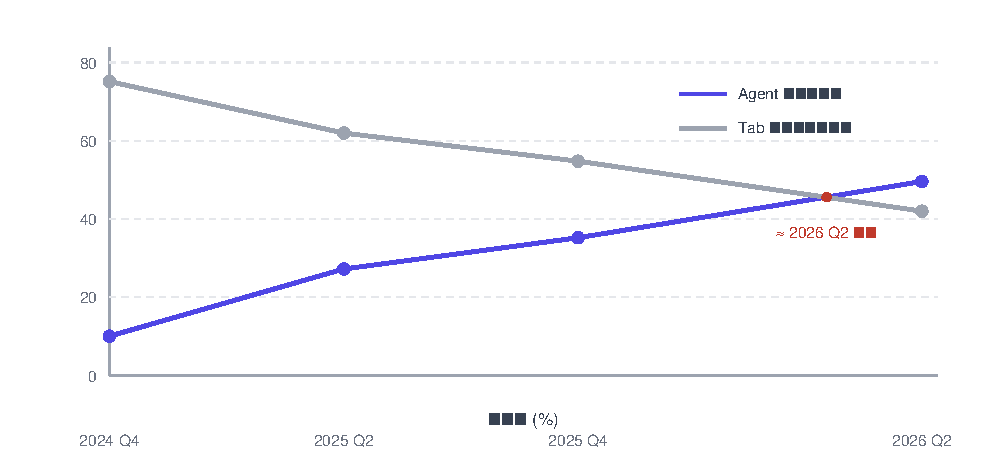
\includegraphics[width=0.92\linewidth]{figures/fig-di-san-shi-qi-zhang-1}
\\[2pt]\small 图 1：AI 编程交互模式使用率变化趋势（基于行业调研数据估算，2026 Q2 Agent 模式反超 Tab 补全）
\end{center}

但说句实在话：工具和模型的变化只是表象。\textbf{无论你用 Cursor 还是 Claude Code，无论底层模型是 GPT-5 还是 Claude 4.5，成功的 AI 编程实践者都在遵循同一套底层方法论}。这就是本指南要教给你的东西。

\booksection{三、核心认知转变：从 Coder 到 Conductor}

传统编程教育教你如何成为一个 Coder——理解语法、记忆 API、调试逻辑错误。AI 编程时代，这个角色正在被重新定义。你不再需要亲手把每一行代码写出来，但你需要成为一个“指挥官”（Conductor）：\textbf{定义战场、制定规则、分配任务、验收成果}。

这个转变的核心不在于“你会不会写代码”，而在于“你会不会想清楚要做什么”。一个优秀的指挥官不一定是最好的士兵，但他必须最清楚战役的目标、地形和兵力部署。同理，一个优秀的 AI 编程实践者不一定精通每一种编程语言的语法细节，但他必须最清楚项目的目标、架构约束和质量标准。

这张表值得你多看两遍——它概括了这次角色转变的全部内涵：

\begin{center}
\begin{tabularx}{\linewidth}{|X|X|X|}
\hline
\textbf{维度} & \textbf{传统 Coder} & \textbf{AI 指挥官（Conductor）} \tabularnewline
\hline
核心技能 & 语法记忆、API 调用、调试 & 需求定义、上下文管理、验收判断 \tabularnewline
工作方式 & 逐行编写代码 & 描述意图，审查产出 \tabularnewline
质量把控 & 自己写的，自己心里有数 & 通过测试和审查验证 AI 产出 \tabularnewline
知识要求 & 深度掌握特定语言/框架 & 广度理解技术全貌，深度理解业务逻辑 \tabularnewline
瓶颈所在 & 编码速度和语法记忆 & 思考清晰度和表达能力 \tabularnewline
错误来源 & 语法错误、逻辑遗漏 & 需求模糊、上下文不足 \tabularnewline
\hline
\end{tabularx}
\end{center}

\begin{center}\small\color{gray}传统 Coder 与 AI 指挥官的能力维度对比\end{center}

这绝不是说编程知识不重要了。恰恰相反：当你能看懂 AI 写的代码时，你才能有效地审查和修正它；当你理解数据结构和算法时，你才能判断 AI 的方案是否合理。\textbf{知识储备决定了你的“指挥上限”——但知识的角色从“执行工具”变成了“判断依据”}。

\booksection{四、为什么方法论比工具更重要}

工具每三个月迭代一次，方法论每三年才进化一次。学会一个工具的操作，三个月后可能就过时了；掌握一套思维方式，三年后依然适用。

很多人在入门 AI 编程时，第一件事就是追问“哪个工具最好”“哪个模型最强”。这些问题不是不重要，但它们问错了优先级。2026 年 8 月的工具格局和 2025 年 8 月已经完全不同——Trae、Qoder 等工具兴衰起伏，Cursor 从插件变成了独立 IDE 又进化到 Cursor 3，Claude Code 从实验性项目变成了终端编程的主流选择。但在这剧烈变化背后，\textbf{成功实践者遵循的思维原则几乎没有改变}。

这就是为什么本书不会把篇幅花在教你某个工具的具体操作上——那些内容写完就会过时。相反，本书的全部重心放在一套经过验证的思维方法论上：如何思考需求、如何与 AI 沟通、如何验证产出、如何持续迭代。\textbf{掌握了这套方法论，你换任何工具都能快速上手；只学了工具操作，换一个工具就要从零开始}。

\begin{tcbinfo}{给零基础读者的定心丸}
如果你是零基础，别被“方法论”三个字吓到。方法论不是抽象的哲学，它就是一套“遇到问题该怎么想”的操作手册。就像学做菜：你可以照着菜谱一步步来（工具操作），但真正的大厨理解的是“为什么要这样调味”“火候怎么控制”（方法论）。本书会从最基础的概念讲起，每个原则都配具体的对比案例，确保你不仅理解“是什么”，更能掌握“怎么做”。

\end{tcbinfo}

\begin{tcbpractice}{来动手：给现在的你拍张"角色照"}
拿出一张纸，写下三个问题的答案：(1) 你现在是怎么用 AI 帮你写代码的（如果用过的话）？(2) 你更像上表中的“Coder”还是“指挥官”？(3) 你希望三个月后的自己会怎样描述自己的工作方式？写完后夹在书里，读完第四十七章再回来看——你会发现变化比想象中快。

\end{tcbpractice}

\begin{tcbsummary}{本章小结}
\begin{itemize}
  \item 2025 年 Karpathy 用"Vibe Coding"命名了 AI 编程革命：从逐行写代码，变成用自然语言描述意图
  \item 2026 年进化到 Agentic Engineering：给目标、放权、AI 自主规划执行，人负责验收
  \item Cursor 3 的 Agent 模式使用率首次反超 Tab 补全；Claude Code 年化收入达 25 亿美元
  \item 你的新角色是 Conductor（指挥官）：定义战场、制定规则、分配任务、验收成果
  \item 工具每三个月迭代一次，方法论每三年才进化一次——学方法论，不学操作
\end{itemize}

\end{tcbsummary}

\bookchapter{第三十八章：AI编程五大思维原则}

\chapterintro{如果这本书只能让你记住一章，那必须是这一章。五大思维原则是全书的心脏，后面所有章节——上下文、需求、对话、质量——都是这五条原则在不同场景下的展开。放心，每一条都不难懂，但每一条都值得你用几个项目去“长进肌肉里”。}

故事的起点很有意思：Andrej Karpathy 在开源他的项目时，附了一份仅\textbf{70 行}的 CLAUDE.md 文件，总结了与 AI 协作的四条核心原则。这份文件在 GitHub 上获得了超过 70,000 个 Star，成为全球 AI 编程实践者最广泛引用的准则。这四条原则不是空洞的口号，而是从大量实践中提炼出的、可操作的思维习惯。\textbf{本书在其基础上补充了第五条——迭代验证——构成完整的五大原则体系}。

\begin{tcbinfo}{70 行文件为什么这么值钱？}
70,000 个 Star 是什么概念？GitHub 上绝大多数项目一辈子都到不了这个数字。一个 70 行的文本文件能获得它，恰恰证明了一件事：AI 时代最稀缺的不是代码，而是“想清楚”的能力。这 70 行，就是“想清楚”的浓缩版。

\end{tcbinfo}

\booksection{一、原则一：Think Before Coding（先思考，再编码）}

这是五条原则中最反直觉的一条。既然 AI 能帮我们写代码，为什么还要“先思考”？答案很简单：\textbf{AI 的产出质量与你的输入质量正相关}。你自己都没想清楚要做什么，AI 给出的答案只会让你陷入无休止的“改了又改”循环——俗称“AI 陪你一起迷路”。

“先思考”意味着在给 AI 下达指令之前，你需要回答三个问题，它们构成一个缺一不可的“思考三角”：

\begin{enumerate}
  \item \textbf{我要解决什么问题？}（目标）
  \item \textbf{我期望的结果长什么样？}（验收标准）
  \item \textbf{有哪些约束条件需要遵守？}（边界）
\end{enumerate}

\begin{center}
\begin{tabularx}{\linewidth}{|X|X|X|}
\hline
\textbf{思考维度} & \textbf{模糊输入（差）} & \textbf{清晰输入（好）} \tabularnewline
\hline
问题定义 & 帮我做个网站 & 帮我做一个个人工具站，展示 3 个 AI 小工具的入口卡片 \tabularnewline
期望结果 & 好看一点 & 响应式布局，暗色主题，卡片有悬停动画，移动端可用 \tabularnewline
约束条件 & （未说明） & 不使用框架，纯 HTML+CSS+JS，单文件部署，不需要后端 \tabularnewline
\hline
\end{tabularx}
\end{center}

\begin{center}\small\color{gray}同一需求的模糊输入与清晰输入对比\end{center}

\begin{tcbwarn}{注意：先思考 $\neq$ 先写完美文档}
“先思考”不等于“写一份完美的 PRD 再开始”。它是一个快速但有条理的思考过程——花 30 秒想清楚上面三个问题，远比花 30 分钟在对话中反复修改来得高效。小任务三问可以很短；大项目可以把它们扩展成完整的需求文档（详见第四十章）。

\end{tcbwarn}

\booksection{二、原则二：Simplicity First（简单至上）}

AI 编程最大的陷阱不是“做不出来”，而是\textbf{“做得太多”}。当你对 AI 说“做一个用户管理系统”，它可能会生成认证、权限、角色、审计日志、数据导出等一整套功能——但你现在可能只需要一个简单的登录页面。过度生成，是 AI 代码膨胀的主要原因。

“简单至上”要求你在每次下达指令时都遵循“最小可行”原则：\textbf{用最少的代码实现核心功能，用最简单的方案解决问题，用最少的功能验证想法}。Karpathy 对此有个精辟的比喻：“如果你要计算一个折扣价格，你不需要一个电商引擎。”

在实践中，“简单至上”意味着几个具体的操作习惯：

\begin{itemize}
  \item 每次只让 AI 实现\textbf{一个功能点}，而不是一口气描述整个系统；
  \item 优先选择标准库和简单方案，而不是引入复杂的依赖；
  \item 能用 50 行代码解决的问题，不要让 AI 写 500 行；
  \item 当 AI 的产出超出预期范围时，勇敢地告诉它"\textbf{砍掉多余的部分}"。
\end{itemize}

\begin{center}
\begin{tabularx}{\linewidth}{|X|X|X|}
\hline
\textbf{场景} & \textbf{过度方案（避免）} & \textbf{简单方案（推荐）} \tabularnewline
\hline
需要存储数据 & 搭建 MySQL 数据库 + ORM & 先用 JSON 文件或 SQLite \tabularnewline
需要用户登录 & OAuth2.0 + JWT + 角色权限 & 先做简单的密码验证 \tabularnewline
需要前端框架 & React + Redux + Router & 先试纯 HTML + 原生 JS \tabularnewline
需要部署上线 & Docker + CI/CD + K8s & 先在本地跑通再说 \tabularnewline
\hline
\end{tabularx}
\end{center}

\begin{center}\small\color{gray}常见场景的过度方案与简单方案对比\end{center}

\booksection{三、原则三：Surgical Changes（精准修改）}

当你在迭代一个已有项目时，每次修改都应该像外科手术一样精准——\textbf{只动该动的地方，不碰不该碰的}。这一点在 AI 编程中尤其重要，因为 AI 有“顺手改一下”的倾向：你让它修一个 bug，它可能顺便重构了半个文件。

“精准修改”的核心要求是：每次给 AI 的指令，都明确指定修改的范围和边界。告诉它“只修改\texttt{calculate\_discount}函数”“不要动其他部分”“保持现有的代码风格”。当 AI 的修改超出了你要求的范围时，立即要求它回退多余的部分。

Karpathy 用一个 diff（差异对比）的例子说明了这一点。假设你让 AI 给购物车的折扣计算函数添加“会员价”逻辑：好的产出是只修改这一个函数、增加几行代码；坏的产出是把整个文件重构了一遍——虽然新代码可能更“优雅”，但你无法确定它有没有引入新 bug。\textbf{在 AI 编程中，“看起来更好”永远不能成为偏离指令的理由}。

差的指令（范围模糊）

\begin{lstlisting}
帮我优化这个项目的
折扣计算逻辑
\end{lstlisting}

好的指令（精准指定范围）

\begin{lstlisting}
只修改 cart.py 中的 calculate\_discount 函数：
1. 在现有折扣基础上增加会员价逻辑
2. 会员用户额外享受 10\% 折扣
3. 不要修改函数签名和其他函数
4. 保持现有的变量命名风格
\end{lstlisting}

\booksection{四、原则四：Goal-Driven Execution（目标驱动执行）}

这条原则回答了一个关键问题：你应该给 AI 下达\textbf{“怎么做”}的指令，还是\textbf{“做什么”}的指令？Karpathy 的答案是后者。与其告诉 AI“先创建一个类，然后添加方法，然后写测试”，不如告诉它“我需要一个能解析 CSV 文件并统计每列唯一值数量的工具”。\textbf{让 AI 自己决定实现路径，你负责验收结果}。

“目标驱动”的好处是双重的。对 AI 来说，它获得了更大的自主空间，可以选择最优的实现路径，而不是被你的中间步骤束缚；对你来说，你把注意力从“怎么做”转移到了“做出来对不对”——这正是指挥官该做的事。

\begin{tcbwarn}{注意：目标驱动 $\neq$ 放任不管}
它需要你在 AI 执行后进行严格的验收：结果是否满足需求？边界情况是否处理了？是否有明显的过度设计？如果结果不符合预期，提供具体的反馈——不是“重写”，而是“这里的问题在于空列表输入会报 IndexError，请修改为添加空值检查”。

\end{tcbwarn}

\begin{center}
\begin{tabularx}{\linewidth}{|X|X|X|}
\hline
\textbf{指令风格} & \textbf{示例} & \textbf{结果特点} \tabularnewline
\hline
命令式（怎么做） & "先创建一个 Python 类，叫 DataParser，加一个 parse 方法，接收 filename 参数，用 csv 模块读取…" & AI 变成打字员，你的中间步骤可能不是最优路径 \tabularnewline
目标式（做什么） & "我需要一个工具：读取 CSV 文件，统计每列的唯一值数量，输出为 JSON 格式。请给出完整实现。" & AI 自主选择最优路径，你负责验收结果 \tabularnewline
\hline
\end{tabularx}
\end{center}

\begin{center}\small\color{gray}命令式指令与目标式指令的对比\end{center}

\booksection{五、原则五：Iterate and Verify（迭代验证）}

这是本书在 Karpathy 四原则基础上补充的第五条。它的核心信念是：\textbf{AI 的第一次产出几乎永远不是最终版本}。有效的 AI 编程是一个“生成-验证-修正”的迭代循环，而不是一次性的“指令-产出”。

“迭代验证”不是被动的“不对就再试”，而是一个有结构的验证流程。每次 AI 给出产出后，按三个层次进行验证：

\begin{itemize}
  \item \textbf{第一层·功能验证}：它能不能跑？输入输出对不对？
  \item \textbf{第二层·边界验证}：空输入、超长输入、异常输入会怎样？
  \item \textbf{第三层·架构验证}：代码结构是否合理？有没有硬编码？是否便于后续扩展？
\end{itemize}

定义目标

AI 生成代码

功能验证

通过

边界验证

通过

架构审查

通过，进入下一步

不通过

提供具体反馈

重新生成

\begin{center}\small\color{gray}图 2：AI 编程的迭代验证循环\end{center}

这个循环的关键在于“提供具体反馈”这一步。当验证不通过时，不要说“不对，重做”，而要说“函数在输入空列表时报 IndexError，请在第 15 行添加空值检查”。\textbf{具体的反馈让 AI 能精准修正；模糊的反馈只会让它重新猜测你的意图}。

\booksection{六、Harness Engineering：Agent = Model + Harness}

2026 年中期，一个叫\textbf{Harness Engineering}的概念开始在 AI 编程社区流行。它的核心公式很简单：

Agent 的能力 = 模型能力 × Harness 质量

模型能力是 AI 大脑的智力上限；Harness 是围绕模型搭建的“工作环境”——包括上下文管理、工具集成、流程编排、记忆系统等。

这个概念解释了一个常见的困惑：为什么同样用 GPT-4 或 Claude，有的人能做出惊艳的项目，有的人只能得到平庸的代码？\textbf{区别不在模型，而在 Harness}。一个好的 Harness 包括：清晰的项目规范文件、合理的工具集成、有条理的对话上下文、完善的验证流程。模型决定了智力上限，Harness 决定了你能多大程度地发挥这个上限。

\begin{tcbinfo}{天才实习生比喻}
你可以把模型想象成一个天才实习生——智商很高，但如果不给他项目背景文档、不告诉他用哪些工具、不给他设定期限和验收标准，他也做不出好东西。Harness Engineering 就是“如何给天才实习生搭好工作环境”的工程。

\end{tcbinfo}

本书的后续章节，本质上都在教你如何构建一个好的 Harness：第三十九章教你管理上下文（项目记忆系统），第四十章教你定义需求（PRD），第四十三章教你对话技术（Prompt 分层），第四十五章教你质量保障（验证流程）。这些组合起来，就是你的 Harness。

\begin{tcbpractice}{来动手：用"思考三角"拆解你的下一个想法}
挑一个你一直想做但没动手的小东西（比如一个倒数日网页、一个喝水提醒脚本）。花 3 分钟回答：(1) 它解决什么问题？(2) 做出来长什么样？(3) 有什么约束（时间、技术、环境）？然后把答案写成一段话。恭喜你，你已经完成了人生第一次“Think Before Coding”——这段话就是一条合格的高质量指令。

\end{tcbpractice}

\begin{tcbsummary}{本章小结}
\begin{itemize}
  \item 五大原则源自 Karpathy 70 行的 CLAUDE.md（70K+ Star），本书补充第五条"迭代验证"
  \item Think Before Coding：开口前回答三问——做什么？结果长啥样？有什么约束？
  \item Simplicity First：AI 最大的坑是"做得太多"——算折扣不需要电商引擎
  \item Surgical Changes：像外科手术一样精准修改，拒绝 AI 的"顺手改一下"
  \item Goal-Driven Execution：说"做什么"，不说"怎么做"，让 AI 自主选路径
  \item Iterate and Verify：三层验证（功能/边界/架构）+ 具体反馈，循环迭代
  \item Harness Engineering：能力 = 模型 × Harness，把 AI 当"天才实习生"来管理环境
\end{itemize}

\end{tcbsummary}

\bookchapter{第三十九章：上下文工程——让AI理解你的意图}

\chapterintro{你有没有过这种体验：换个新对话窗口，AI 就像失忆了一样，把你项目的基本情况全忘了？这不是 AI 故意气你，而是它天生“健忘”。这一章教你给 AI 装上一套“长期记忆系统”，顺便认识 2026 年最火的开发范式之一——规范驱动开发。}

\booksection{一、项目记忆文件：AI 的“长期记忆”}

AI 模型有一个根本性限制：\textbf{它的记忆是“短时”的}。每次对话开始时，AI 对你项目的了解为零。你需要在对话中不断告诉它“我们用的是 React”“后端是 Node.js”“数据库是 PostgreSQL”“代码风格用双引号”。这不仅低效，而且容易遗漏——就像每天都要重新给新来的同事做入职培训。

解决方案是“项目记忆文件”——一个放在项目根目录的纯文本文件，AI 工具会在每次对话开始时自动读取它。不同的工具有不同的命名约定：

\begin{center}
\begin{tabularx}{\linewidth}{|X|X|}
\hline
\textbf{工具} & \textbf{文件名} \tabularnewline
\hline
Cursor & \texttt{.\allowbreak cursorrules} \tabularnewline
Claude Code & \texttt{CLAUDE.\allowbreak md} \tabularnewline
GitHub Copilot & \texttt{copilot-\allowbreak instructions.\allowbreak md} \tabularnewline
通用方案 & \texttt{AGENTS.\allowbreak md} \tabularnewline
\hline
\end{tabularx}
\end{center}

\begin{center}\small\color{gray}各工具的项目记忆文件命名约定\end{center}

虽然命名不同，但原理一样：\textbf{把你希望 AI“始终记住”的信息写在这个文件里}。一个好的项目记忆文件应该包含：项目概述（这是什么项目）、技术栈（用了什么技术）、代码规范（命名、缩进、注释风格）、目录结构（代码怎么组织的）、开发约定（分支策略、提交规范、测试要求）。Karpathy 的 CLAUDE.md 只有 70 行，但覆盖了所有关键信息——简洁但完备。

\begin{lstlisting}
# 项目：个人记账应用
## 概述
这是一个全栈个人记账应用，帮助用户记录日常收支。
## 技术栈
- 前端：React + TypeScript + Tailwind CSS
- 后端：Node.js + Express + TypeScript
- 数据库：SQLite (开发) / PostgreSQL (生产)
- 测试：Vitest
## 代码规范
- 使用双引号
- 缩进2个空格
- 函数名用camelCase
- 类型定义用PascalCase
- 每个函数必须有JSDoc注释
## 目录结构
/src
  /frontend  - 前端代码
  /backend   - 后端代码
  /shared    - 前后端共享的类型
  /tests     - 测试文件
## 开发约定
- 提交信息用中文
- 新功能必须先写测试
- API返回统一用 { success, data, error } 格式
\end{lstlisting}

\begin{tcbwarn}{注意：别写成"第二份需求文档"}
注意这个文件的长度——不要写成几十页的需求文档。项目记忆文件的目的是“让 AI 快速建立背景认知”，不是“详细描述每个功能”。保持简洁、结构化、只写“AI 需要知道的”。

\end{tcbwarn}

\booksection{二、规范驱动开发（SDD）}

\textbf{Spec-Driven Development}（SDD，规范驱动开发）是 2026 年逐渐成熟的一种开发范式，核心理念一句话：\textbf{先写规范，再写代码}。与传统 TDD（测试驱动开发）不同的是，SDD 的“规范”不仅是测试用例，还包括需求描述、接口定义、数据模型等。AI 根据这些规范来生成代码，人类的职责是编写和维护规范。

SDD 的工作流程五步走：

\begin{enumerate}
  \item 用自然语言描述需求规范（写在一个 .md 文件中）；
  \item 定义接口和数据结构（写在规范文件中）；
  \item 让 AI 根据规范生成代码实现；
  \item 运行测试验证产出是否符合规范；
  \item 如果不符合，修正规范或让 AI 修正代码。
\end{enumerate}

在这个流程中，\textbf{规范文件是“唯一真理源”——代码可以重新生成，但规范必须先正确}。

编写规范文件

审查规范是否完备？

完备

AI 根据规范生成代码

运行测试验证产出

不完备 / 测试不过

代码问题 修正代码；规范问题 修正规范

回到验证

全部通过 交付

\begin{center}\small\color{gray}图 3：规范驱动开发（SDD）的工作流程\end{center}

SDD 的优势在于：\textbf{规范文件比代码更稳定}。当底层模型或工具变化时，你的规范文件依然有效，只需要让新的 AI 工具重新生成代码即可。这也是为什么本书强调“方法论比工具重要”——规范文件就是你方法论的具体载体。

\booksection{三、上下文窗口管理}

即使有了项目记忆文件，你仍然会在对话中遇到“上下文不够用”的问题。AI 模型的上下文窗口（能同时处理的信息量）是有限的。当对话太长、引用的文件太多时，AI 会“忘记”早期的信息，导致产出质量下降——就像你和一个朋友聊天聊了六个小时，他早忘了你开头说的第一件事。

管理上下文窗口的核心策略是“分层引用”：

\begin{center}
\begin{tabularx}{\linewidth}{|X|X|X|}
\hline
\textbf{上下文层次} & \textbf{内容} & \textbf{管理方式} \tabularnewline
\hline
第一层：项目记忆 & 技术栈、规范、目录结构 & 写在 CLAUDE.md 等文件中，自动加载，无需重复 \tabularnewline
第二层：文件引用 & 当前任务涉及的代码文件 & 用 @ 符号精确引用，不粘贴全文到对话 \tabularnewline
第三层：对话上下文 & 当前任务的对话历史 & 完成一个任务后开新对话，避免上下文膨胀 \tabularnewline
第四层：即时指令 & 当前这一步的具体要求 & 清晰、简洁、有针对性，避免冗长描述 \tabularnewline
\hline
\end{tabularx}
\end{center}

\begin{center}\small\color{gray}上下文窗口的分层管理策略\end{center}

\booksection{四、上下文工程的实践要点}

上下文工程不是一次性的设置，而是一个持续优化的过程。以下是几个在实践中被反复验证的要点：

\begin{enumerate}
  \item \textbf{记忆文件随项目演进同步更新}。引入新技术或改变架构时，第一时间更新记忆文件，而不是在对话中临时说明。
  \item \textbf{善用 @ 引用而非全文粘贴}。大多数 AI 编程工具支持 @file 或 @folder 语法，它会在后台将文件内容注入 AI 的上下文，比手动粘贴更高效且不会污染对话。
  \item \textbf{对话要"短小精悍"}。一个对话只处理一个任务或一个功能点。完成后开新对话处理下一个。长对话不仅消耗上下文窗口，还会让 AI"分心"。
  \item \textbf{给 AI"看"结果而非"描述"结果}。遇到 bug 时，把错误日志直接 @ 引用给 AI，而不是用自己的话描述"好像有个什么错误"。AI 看到原始信息比看到你的转述更有效。
  \item \textbf{定期清理和归档}。已完成的对话和临时文件会占用工作空间。定期清理无关内容，保持项目目录整洁，也有助于 AI 更高效地理解项目结构。
\end{enumerate}

\begin{tcbpractice}{来动手：给你的项目写一份 70 行记忆文件}
挑一个你正在做（或打算做）的项目，写一份 CLAUDE.md：项目概述（2-3 句话）、技术栈（列出来）、代码规范（3-5 条）、目录结构（画个树）、开发约定（2-3 条）。控制在 70 行以内——写完你会发现自己对项目的理解都清晰了不少。

\end{tcbpractice}

\begin{tcbsummary}{本章小结}
\begin{itemize}
  \item AI 的记忆是"短时"的：每次新对话，它对项目的了解为零
  \item 项目记忆文件（CLAUDE.md 等）是 AI 的"长期记忆"，每次对话自动加载
  \item 好的记忆文件 = 概述 + 技术栈 + 规范 + 目录 + 约定，70 行足矣
  \item SDD 规范驱动开发：先写规范再写代码，规范是"唯一真理源"，比代码更稳定
  \item 上下文分四层管理：项目记忆 @文件引用 对话历史 即时指令
  \item 五个实践要点：同步更新、@引用、短对话、给原信息、定期清理
\end{itemize}

\end{tcbsummary}

\bookchapter{第四十章：需求工程——把想法变成AI可执行的指令}

\chapterintro{如果说上下文工程解决的是“让 AI 了解背景”，那需求工程解决的是“让 AI 知道这次具体要做什么”。这是 AI 编程中最能体现人与人差距的环节——同样的工具、同样的模型，有人能做出令人惊艳的项目，有人只能做出平庸的玩具。区别往往不在技术能力，而在\textbf{需求表达能力}。}

\booksection{一、从模糊想法到结构化需求}

每个项目都始于一个模糊的想法——“我想做一个记账 App”“我想做个个人网站”“我想做个待办清单工具”。这些想法本身没有问题，但如果你直接把它丢给 AI，产出的质量完全取决于运气。需求工程的目标，就是把这个模糊的想法，变成一个 AI 能精确执行的结构化需求。

好消息是：结构化需求不需要你写一份几十页的 PRD。它只需要你回答五个问题，我们称之为\textbf{“需求五要素”}：

\begin{center}
\begin{tabularx}{\linewidth}{|X|X|X|}
\hline
\textbf{要素} & \textbf{问题} & \textbf{示例：记账 App} \tabularnewline
\hline
Who & 给谁用？ & 个人使用，记录日常收支 \tabularnewline
What & 做什么？ & 一个能记录每笔收支、按月汇总、可视化的应用 \tabularnewline
Why & 为什么做？ & 想了解自己的消费结构，找出不必要的支出 \tabularnewline
How & 大致怎么做？ & 前端用 React，数据存浏览器本地，先不做后端和登录 \tabularnewline
Constraint & 有什么限制？ & 单人开发，2 周内完成，不需要上线部署 \tabularnewline
\hline
\end{tabularx}
\end{center}

\begin{center}\small\color{gray}需求五要素及示例\end{center}

这五个要素不需要写成正式文档，甚至在脑海中快速过一遍就足够了。关键是养成“先想清楚再开口”的习惯。你会发现，当你能清晰地回答这五个问题时，你的需求描述自然就变得结构化了。

\booksection{二、需求拆解的分层艺术}

对于较大的项目，一个需求描述是不够的。你需要把大需求拆解成小的、可独立验证的子需求。这个过程叫做“需求拆解”，核心原则是：\textbf{每个子需求都应该能独立完成、独立验证、独立交付}。

以“做一个个人记账 App”为例，一个合理的拆解方式是：

\begin{enumerate}
  \item 实现基础的收支记录功能（能添加、查看、删除记录）；
  \item 添加分类功能（给每笔记录打上餐饮、交通等标签）；
  \item 实现月度汇总功能（按月统计收支情况）；
  \item 添加数据可视化（用图表展示消费结构）。
\end{enumerate}

每一步都是一个可以独立运行和验证的功能增量。

需求拆解的黄金法则：每一步完成后，项目都应该是一个"能用的东西"——哪怕功能很简陋。永远不要让项目停留在"什么都做了一半但什么都用不了"的状态。

这种拆解方式有两个好处。首先，它让你始终能看到进展——每完成一步，你的 App 就多了一个功能，这种正反馈对于长期项目至关重要（人都是需要成就感的嘛）。其次，它让 AI 的每次任务都足够小，降低了“AI 理解偏差”的风险——任务越小，AI 的理解越准确，产出质量越高。

\booksection{三、PRD 写作模板与实践}

对于较大的项目（比如一个有前后端、多个功能模块的全栈应用），仅凭需求五要素可能不够。这时你需要写一份更正式的项目需求文档（PRD）。一个容易误解的点是：\textbf{PRD 不是写给 AI 看的——它是写给你自己的}，帮你理清思路，然后你才能给 AI 提供更精确的指令。

一份好的 PRD 不需要很长，但应该包含六个部分：项目概述（一段话说清楚做什么）、功能列表（每个功能点是什么）、技术方案（用什么技术栈、大致架构）、数据模型（核心数据结构）、界面描述（主要页面长什么样）、开发计划（分几步完成）。

\begin{lstlisting}
# 个人记账应用 PRD
## 项目概述
一个轻量级个人记账应用，支持收支记录、分类、月度汇总和数据可视化。
## 功能列表
1. 记录收支：金额、类型(收入/支出)、分类、备注、日期
2. 分类管理：预设餐饮、交通、购物、娱乐、其他
3. 月度汇总：按月统计总收入、总支出、结余
4. 消费可视化：饼图展示各分类占比
5. 数据导出：导出为CSV
## 技术方案
- 前端：React + TypeScript + Tailwind CSS
- 数据存储：localStorage（无需后端）
- 图表：使用Chart.js
- 构建：Vite
## 数据模型
Record {
  id: string
  amount: number
  type: 'income' | 'expense'
  category: string
  note: string
  date: string  // YYYY-MM-DD
}
## 开发计划
Step 1: 基础记录功能 (CRUD)
Step 2: 分类管理
Step 3: 月度汇总
Step 4: 数据可视化
Step 5: 数据导出
\end{lstlisting}

注意这份 PRD 的写作风格：用简洁的列表和结构化的格式，而不是长篇大论。每个功能点都有明确的定义，数据模型用简单的类型描述。这种风格的 PRD 不仅你自己看得清楚，当你把它提供给 AI 时，AI 也能精确理解每个需求点。

\booksection{四、实战：从想法到方案的完整推演}

纸上谈兵没意思，咱们用一个完整的例子走一遍需求工程的全过程。假设你的想法是：\textbf{“我想做一个能追踪我每天学了什么的学习追踪器”}。

\textbf{第一步，过一遍需求五要素。}

\begin{itemize}
  \item Who：个人使用。
  \item What：一个能记录每天学习内容、追踪学习时长、回顾学习进度的工具。
  \item Why：想养成持续学习的习惯，看到自己的积累。
  \item How：先做一个网页版，数据存在浏览器本地。
  \item Constraint：零基础开发，1 周内完成核心功能。
\end{itemize}

\textbf{第二步，拆解需求。}

\begin{enumerate}
  \item Step 1：实现"记录学习条目"功能（日期、内容、时长）；
  \item Step 2：添加"学习时长统计"（今日、本周累计）；
  \item Step 3：实现"学习日历"视图（像 GitHub 贡献图一样展示）；
  \item Step 4：添加"学习回顾"功能（随机展示过去某天的学习记录，帮助复习）。
\end{enumerate}

\textbf{第三步，写一份简短 PRD。}不需要长——上面的拆解本身就构成了 PRD 的主体。把它整理成一个 .md 文件，放在项目根目录，作为你和 AI 的共同参考。

\textbf{第四步，开始第一步的开发。}给 AI 的指令可以是：

\begin{lstlisting}
我需要一个学习追踪器的第一个功能——记录学习条目。
用户可以添加一条学习记录，包含日期、学习内容、学习时长（分钟）。
数据存在localStorage。
前端用React + TypeScript。
请给出完整实现。
\end{lstlisting}

注意这个指令的特点：它\textbf{只描述当前这一步的目标}（记录功能），不掺杂其他功能；它\textbf{明确了技术约束}（React、TypeScript、localStorage）；它给了足够的信息让 AI 知道“做什么”和“怎么做”，但具体实现由 AI 决定。这就是一个经过需求工程加工后的、高质量的 AI 编程指令。

\begin{tcbpractice}{来动手：给你的"心头好"写一份五要素卡}
选一个你酝酿已久的小项目，花 5 分钟填一张卡：Who / What / Why / How / Constraint，各一句话。然后把它拆成 3-5 个“每一步都能用”的步骤。你会发现：把想法写下来之后，它就从“白日梦”变成了“待办清单”。

\end{tcbpractice}

\begin{tcbsummary}{本章小结}
\begin{itemize}
  \item 需求五要素：Who / What / Why / How / Constraint——想清楚再开口
  \item 需求拆解黄金法则：每一步完成后项目都是"能用的东西"
  \item PRD 是写给自己的：概述、功能列表、技术方案、数据模型、界面、计划
  \item 好指令 = 只描述当前一步 + 明确约束 + 说"做什么"不说"怎么做"
  \item 完整推演模板：五要素 拆解 PRD 给指令，四步走
\end{itemize}

\end{tcbsummary}

\bookchapter{第四十一章：2026年AI编程工具全景}

\chapterintro{先打个预防针：本章是 2026 年 8 月工具生态的一张“快照”。半年后它就会过时——这恰恰是本章想教会你的第一课。本章的目的不是教你“用哪个工具”，而是帮你建立“如何选择工具”的判断框架。当你理解了不同工具的设计哲学，你就能在任何时候做出适合自己的选择。}

\booksection{一、三大流派与选择框架}

2026 年的 AI 编程工具大致分为三大流派，每种流派背后是一种不同的设计哲学。先看这张全景图：

\begin{center}
\begin{tabularx}{\linewidth}{|X|X|X|X|}
\hline
\textbf{流派} & \textbf{代表工具} & \textbf{设计哲学} & \textbf{适合场景} \tabularnewline
\hline
IDE 内置 AI & Cursor 3, Trae, Windsurf, CodeBuddy & 把 AI 能力深度集成到编辑器中 & 日常开发、代码审查、渐进式增强 \tabularnewline
终端 Agent & Claude Code, Codex CLI, Aider & 以终端为界面，AI 直接操作文件系统和命令 & 项目级操作、批量修改、CI/CD 集成 \tabularnewline
云端 Builder & v0, Bolt, Replit Agent & 在浏览器中从零创建完整项目 & 快速原型、零配置上手、即时预览 \tabularnewline
\hline
\end{tabularx}
\end{center}

\begin{center}\small\color{gray}AI 编程工具的三大流派\end{center}

选择工具的关键不是“哪个最好”，而是“\textbf{哪个最适合你当前的场景}”。三个实用的判断维度：

\begin{itemize}
  \item \textbf{你的编程基础如何？}零基础选云端 Builder，有基础选 IDE 内置 AI，高级用户选终端 Agent。
  \item \textbf{你的项目阶段在哪里？}从零开始选云端 Builder，迭代开发选 IDE 内置 AI，维护重构选终端 Agent。
  \item \textbf{你的部署需求是什么？}快速验证选云端 Builder，严肃项目选 IDE 内置 AI，自动化流程选终端 Agent。
\end{itemize}

\booksection{二、IDE 内置 AI 流派}

IDE 内置 AI 是最主流的流派：把 AI 能力嵌入到你的代码编辑器里，在保留传统编程体验的同时叠加 AI 增强。2026 年这个流派的代表是 Cursor 3、Trae、Windsurf 和 CodeBuddy。

\booksubsection{Cursor 3}

Cursor 是目前全球使用最广泛的 AI 编程 IDE。2026 年 4 月发布的 Cursor 3 标志着 AI 编程工具的一个重要转折点：\textbf{Agent 模式的使用率首次超过 Tab 补全模式}——开发者从“AI 帮我补全代码”转向了“AI 帮我完成任务”。Cursor 3 的核心特性包括：多文件编辑（AI 可以同时修改多个文件来完成任务）、上下文感知（自动理解项目结构和依赖关系）、与终端的深度集成（AI 可以在编辑器内直接运行命令和查看输出）。

\booksubsection{Trae}

Trae 是字节跳动推出的 AI 编程 IDE，在国内市场有较大的用户基数。它的 SOLO 模式（也称为 Builder 模式）是典型的“一句话创建项目”能力——你描述需求，AI 自主完成从项目初始化到代码生成的全流程。Trae 的优势在于\textbf{中文支持和国内网络环境适配}，适合国内用户快速上手。

\booksubsection{其他工具}

Windsurf（原 Codeium）以流畅的代码补全体验著称，适合追求“打字如飞”体验的开发者。腾讯云 CodeBuddy 作为 VS Code 插件，擅长与云生态集成，适合计划部署到腾讯云或开发微信小程序的项目。阿里通义灵码和百度 Comate 也提供了类似的 IDE 集成体验，各自在中文场景优化上有特色。

\booksection{三、终端 Agent 流派}

终端 Agent 是 2026 年增长最快的流派。核心理念：\textbf{AI 不应该只是一个编辑器插件，它应该能像开发者一样操作整个开发环境}——读写文件、运行命令、查看输出、安装依赖。Claude Code 是这个流派的代表。

\booksubsection{Claude Code}

Claude Code 是 Anthropic 推出的终端 AI 编程工具，到 2026 年中期已达到年化收入 25 亿美元的规模。它的工作方式与传统 IDE 完全不同：你在终端中用自然语言描述任务，Claude Code 会自主读取相关文件、修改代码、运行测试、查看结果、迭代修正——整个过程不需要你打开编辑器。

Claude Code 的优势在于“全项目感知”：它不受编辑器窗口限制，可以自由地浏览整个项目目录，理解文件间的依赖关系。它也支持 CLAUDE.md 项目记忆文件，让 AI 在每次会话开始时就了解项目背景。对于大型项目的重构、批量修改、测试编写等任务，终端 Agent 比 IDE 插件更高效。

\booksubsection{Codex CLI 与 Aider}

OpenAI 的 Codex CLI 提供了类似的终端编程体验，并支持 /import 功能——可以导入现有的代码库让 AI 理解。Aider 是一个开源的终端 AI 编程工具，支持多种模型（GPT、Claude、DeepSeek 等），适合想要灵活切换模型的用户。这些工具虽然各有特色，但核心理念一致：\textbf{让 AI 在终端中拥有完整的开发环境操作能力}。

\booksection{四、云端 Builder 流派}

云端 Builder 是最适合零基础用户的流派。你不需要安装任何软件，只需要打开浏览器，描述你的需求，AI 就会在云端创建完整的项目，并提供即时预览。

\begin{itemize}
  \item \textbf{v0}（Vercel 出品）：擅长生成前端 UI 组件和页面，适合快速制作网页原型。
  \item \textbf{Bolt}：支持从一句话创建全栈应用，包含前端、后端和数据库。
  \item \textbf{Replit Agent}：在 Replit 的云端 IDE 中工作，不仅能创建项目，还能直接在云端运行和部署。
\end{itemize}

这些工具的共同优势是“\textbf{零配置上手}”——打开浏览器就能开始。局限在于：当项目变复杂后，云端编辑环境的灵活性不如本地 IDE。因此它们最适合“从 0 到 1”的原型阶段：用云端 Builder 快速验证想法，验证通过后再迁移到本地 IDE 进行深度开发。

\booksection{五、工具会变，方法论不变}

如果明天所有 AI 编程工具都消失了，你仍然应该保持的三个习惯：先想清楚再动手、每次只做一小步、做完就验证。工具是放大器，方法论是地基。放大器可以替换，地基不能动摇。

回顾 2024 到 2026 年的工具变迁：2024 年 GitHub Copilot 是王者，2025 年 Cursor 取而代之，2026 年 Claude Code 异军突起。每一个新工具出现时，都有人宣称“这次不一样”，但最终发现：\textbf{用好新工具的人，恰恰是那些方法论扎实的人}。他们换工具只需要几天适应期，而只学了工具操作的人换一次就要重新学起。

因此，本书建议的学习路径是：先用一个工具（任何一个都行）入门，在实践中体会五大思维原则；当你的方法论足够扎实后，再尝试不同流派的工具，感受它们的设计哲学差异；最终，你会形成自己的工具组合——比如用 Cursor 做日常开发，用 Claude Code 做重构和测试，用 v0 做快速原型。\textbf{工具组合因人而异，但方法论是共通的}。

\begin{tcbpractice}{来动手：给你自己配一套"兵器组合"}
用三个判断维度（编程基础、项目阶段、部署需求）给自己定位：如果你是零基础 试试 Bolt 或 v0 做一个页面；有基础 用 Cursor 或 Trae 做一个迭代任务；想挑战 在终端里跑一次 Claude Code。然后回答：哪种流派最符合你当前的阶段？

\end{tcbpractice}

\begin{tcbsummary}{本章小结}
\begin{itemize}
  \item 三大流派：IDE 内置 AI（日常开发）、终端 Agent（项目级操作）、云端 Builder（零基础原型）
  \item 选工具看三问：编程基础？项目阶段？部署需求？
  \item Cursor 3 的 Agent 模式首次反超 Tab 补全；Claude Code 年化收入 25 亿美元
  \item 云端 Builder 适合"从 0 到 1"，验证后迁回本地 IDE 深度开发
  \item 工具每三个月迭代一次：学方法论的人换工具只需几天适应期
\end{itemize}

\end{tcbsummary}

\bookchapter{第四十二章：大模型全景与API实战}

\chapterintro{前面几章讲的都是“怎么和 AI 协作”，本章解决一个更基础的问题：“用哪个 AI？怎么用？”2026 年 8 月的大模型格局已经极其丰富——国际有 GPT、Claude、Gemini 三强争霸，国内有 DeepSeek、通义千问、GLM、Kimi、豆包百花齐放。每个模型都有自己的性格和特长：选对了事半功倍，选错了事倍功半。本章不仅带你认识这些模型，还会教你如何通过 API 将它们接入自己的应用，以及如何根据自己的需求选择合适的 Token Plan（用量套餐）。}

\booksection{一、国际主流大模型：三强格局}

2026 年 8 月的国际大模型市场，形成了 OpenAI（GPT 系列）、Anthropic（Claude 系列）、Google（Gemini 系列）三强鼎立的格局。每家都有自己鲜明的特色——咱们一个一个认识。

\booksubsection{OpenAI GPT-5.6 系列：全能均衡的六边形战士}

OpenAI 是大模型浪潮的开启者，GPT 系列至今仍是全球使用最广泛的模型。2026 年 7 月发布的 GPT-5.6 系列采用三档定位策略：旗舰款 GPT-5.6 Sol 面向高端推理需求，均衡款 GPT-5.6 Terra 面向日常开发，轻量款 GPT-5.6 Luna 面向高并发低成本场景。三款模型共享 105 万 Token 的上下文窗口，都支持图像输入、函数调用和结构化输出。

\begin{center}
\begin{tabularx}{\linewidth}{|X|X|X|X|X|}
\hline
\textbf{型号} & \textbf{定位} & \textbf{输入(/百万Token)} & \textbf{输出(/百万Token)} & \textbf{上下文窗口} \tabularnewline
\hline
GPT-5.6 Sol & 旗舰推理 & US\$5.00 (约36元) & US\$30.00 (约217元) & 105万Token \tabularnewline
GPT-5.6 Terra & 均衡日常 & US\$2.50 (约18元) & US\$15.00 (约109元) & 105万Token \tabularnewline
GPT-5.6 Luna & 轻量低成本 & US\$1.00 (约7元) & US\$6.00 (约44元) & 105万Token \tabularnewline
\hline
\end{tabularx}
\end{center}

\begin{center}\small\color{gray}OpenAI GPT-5.6 系列定价（2026 年 8 月）\end{center}

GPT 系列的核心优势在于“均衡”——推理、编程、写作、多模态，没有明显短板。加上 OpenAI 庞大的插件生态和开发者社区，适配文档和工具链最为完善。对于“不知道选什么”的场景，GPT 是“闭眼选都不会错”的默认答案。但它的短板是：国内访问需要特殊网络，中文表达偶尔有“翻译腔”，API 价格处于中高水平。

\textbf{好消息}\par

OpenAI 在 2026 年 8 月宣布免费用户默认模型升级为 GPT-5.6 Luna，并开放无限量文本聊天。这意味着你可以零成本体验 GPT 的基础能力，只有在需要更强推理或 API 调用时才需要付费。

\booksubsection{Anthropic Claude 系列：编程与严谨的天花板}

如果说 GPT 是全能选手，那 Claude 就是编程领域的“天花板”。Anthropic 的 Claude 系列在 SWE-bench（软件工程基准测试）上长期断层领先，代码生成质量和工程级项目落地能力业界第一。更难得的是，Claude 的幻觉率（生成虚假信息的概率）全网最低，仅约 1\%——这使它特别适合学术、法务等高精度场景。

Claude 的另一个杀手锏是超长上下文：支持 100 万 Token 的上下文窗口，能一次性“读完”几百页的合同或整个代码库不漏细节。这在代码重构、长文档分析等场景中几乎无可替代。Claude Code 作为终端 AI 编程工具，到 2026 年中期年化收入已达 25 亿美元——这是 Claude 编程能力最受认可的证据。

\begin{center}
\begin{tabularx}{\linewidth}{|X|X|X|X|X|}
\hline
\textbf{型号} & \textbf{定位} & \textbf{输入(/百万Token)} & \textbf{输出(/百万Token)} & \textbf{上下文窗口} \tabularnewline
\hline
Claude Fable 5 & 旗舰款 & US\$10.00 (约72元) & US\$50.00 (约362元) & 100万Token \tabularnewline
Claude Opus 4.8 & 专业款 & US\$5.00 (约36元) & US\$25.00 (约181元) & 100万Token \tabularnewline
Claude Sonnet 5 & 性价比款 & US\$2.00 (约14元) & US\$10.00 (约72元) & 100万Token \tabularnewline
\hline
\end{tabularx}
\end{center}

\begin{center}\small\color{gray}Anthropic Claude 系列定价（2026 年 8 月，Sonnet 5 为优惠价）\end{center}

Claude 的短板是价格——Fable 5 的输出价格是所有模型中最高的，每百万 Token 要 50 美元。多模态能力（图像、视频理解）也相对较弱。对于预算有限的个人开发者，Sonnet 5 在优惠期内的性价比非常突出。

\booksubsection{Google Gemini 系列：多模态的王者}

Google 的 Gemini 系列在 2026 年已迭代至 3.1 Pro 版本。Gemini 的最大杀手锏是原生多模态——图文解析精准、OCR 表格识别无误、视频帧提取高效，还支持音视频深度解析。它与 Google 生态（搜索、邮箱、云服务）深度绑定，在实时信息检索和跨模态理解上表现突出。Gemini 还支持\textbf{200 万 Token}的超长上下文输入，是目前上下文窗口最大的模型。

Gemini 的定位是“科学推理和多模态场景的首选”。如果你的项目涉及大量图像分析、视频理解或科学计算，Gemini 几乎没有对手。但它在纯文本代码生成上略逊于 Claude，中文表达也不如国产模型自然。

\begin{center}
\begin{tabularx}{\linewidth}{|X|X|X|X|}
\hline
\textbf{对比项} & \textbf{GPT-5.6} & \textbf{Claude Fable 5} & \textbf{Gemini 3.1 Pro} \tabularnewline
\hline
综合得分 & 94.8 & 95.0 & 92.1 \tabularnewline
编程能力(SWE-bench) & 74.9\% & 64.3\% (Pro) & 中等 \tabularnewline
上下文窗口 & 105万Token & 100万Token & 200万Token \tabularnewline
多模态能力 & 均衡 & 较弱 & 最强 \tabularnewline
幻觉率 & 较低 & 最低(约1\%) & 较低 \tabularnewline
国内可用性 & 需特殊网络 & 需特殊网络 & 需特殊网络 \tabularnewline
API 生态 & 最完善 & 成长中 & Google 生态绑定 \tabularnewline
\hline
\end{tabularx}
\end{center}

\begin{center}\small\color{gray}国际三大模型横向对比（2026 年 8 月）\end{center}

\begin{tcbwarn}{注意：国内使用的现实门槛}
对于国内开发者来说，GPT、Claude、Gemini 的核心障碍是网络访问。虽然可以通过 Azure 代理、API 聚合平台等方式间接使用，但稳定性和合规性需要自行评估。如果你的项目对数据安全有严格要求，建议优先考虑国产模型。

\end{tcbwarn}

\booksection{二、国产主流大模型：百花齐放}

2026 年的国产大模型已经从“追赶者”变成了“并跑者”，在某些领域甚至实现了“领跑”。与 2023 年“套壳”争议不同，2026 年的国产旗舰模型在逻辑推理、代码生成、中文理解等方面已经与国际一线模型旗鼓相当，差距缩减到 5\% 以内。更重要的是，国产模型在中文场景、价格成本和合规部署上有不可替代的优势。

\booksubsection{DeepSeek V4：性价比之王}

DeepSeek（深度求索）是国产大模型中现象级的存在。2025 年初，DeepSeek-V3 以“比 GPT 便宜十分之一但能力相当”的定位震撼市场，被业内称为“通用 AI 大模型斩杀线”——\textbf{比它便宜的没它好用，比它贵的没它量大管饱}。到 2026 年 8 月，DeepSeek V4-Pro 正式版发布：1.6 万亿参数 MoE 架构，激活约 49B，支持 100 万无损上下文，代码性价比被广泛认为是全球天花板。

DeepSeek V4 在 Agent 能力上实现了大幅跃升——DeepSWE 基准从 12.8 跳至 62.7（+390\%），NL2Repo 从 38.5 升至 61.5。API 新增了 Responses API 与 Anthropic API 双协议支持，已兼容 Codex 和 Claude Code 等主流编程工具。这意味着你可以用 DeepSeek 的 API 替代 Claude 的 API，在 Claude Code 中使用——\textbf{成本降低数倍，体验几乎一致}。

\begin{center}
\begin{tabularx}{\linewidth}{|X|X|X|X|X|}
\hline
\textbf{型号} & \textbf{定位} & \textbf{输入(/百万Token)} & \textbf{输出(/百万Token)} & \textbf{上下文窗口} \tabularnewline
\hline
DeepSeek V4 Pro & 旗舰推理 & 3元 (约US\$0.43) & 6元 (约US\$0.87) & 100万Token \tabularnewline
DeepSeek V4 Flash & 轻量快速 & 1元 (约US\$0.14) & 2元 (约US\$0.28) & 100万Token \tabularnewline
\hline
\end{tabularx}
\end{center}

\begin{center}\small\color{gray}DeepSeek V4 系列定价（2026 年 8 月，促销价）\end{center}

价格对比：同样 100 万 Token 的输入 + 100 万 Token 的输出，DeepSeek V4 Flash 花费约 0.42 美元，GPT-5.6 Sol 花费约 35 美元，Claude Fable 5 花费约 60 美元。\textbf{差距高达 80-140 倍}。

\textbf{避坑提醒：DeepSeek 要涨价了}\par

DeepSeek 官方已于 2026 年 8 月 6 日公告“计划近期大幅上调 API 定价”，促销价可能不会持续太久。部分媒体传闻涨幅可能达 30 倍，截至 8 月 14 日官方尚未公布最终调价方案。此外，DeepSeek V4 正式版引入了\textbf{峰谷定价机制}——高峰时段调用价格直接翻倍。建议关注官方公告获取最新定价。

\booksubsection{通义千问 Qwen3.7 Max：阿里云的企业级选择}

阿里云的通义千问（Qwen）系列依托阿里云生态，在企业级部署上有天然优势。2026 年 7 月的 Qwen3.7 Max 是当前旗舰：235B 参数稠密模型，256K 原生上下文，可扩展至 1M。Qwen 的核心优势在于：开源生态成熟（从 7B 到 235B 全系列开源）、中文场景理解精准、与阿里云基础设施深度集成。

\begin{center}
\begin{tabularx}{\linewidth}{|X|X|X|}
\hline
\textbf{型号} & \textbf{输出价格(/百万Token)} & \textbf{适用场景} \tabularnewline
\hline
qwen-turbo & 0.6元 & 极简问答、文本分类、高并发 \tabularnewline
qwen-long & 2.0元 & 10M 超长上下文处理 \tabularnewline
qwen3.7-flash & 7.2元 & 通用对话、内容生成 \tabularnewline
qwen3.7-plus & 12.0元 & 多模态（图片+视频）、中文创作 \tabularnewline
qwen3.7-max & 36.0元 & 旗舰中文能力、复杂任务 \tabularnewline
\hline
\end{tabularx}
\end{center}

\begin{center}\small\color{gray}通义千问 Qwen 系列阶梯定价（2026 年 8 月）\end{center}

Qwen 的定价采用阶梯策略——从极低成本的 qwen-turbo（输出 0.6 元/百万 Token）到旗舰 qwen3.7-max（输出 36 元/百万 Token），覆盖从轻量问答到复杂推理的全场景需求。对于已经在使用阿里云的企业，Qwen 是最顺手的集成选择。

\booksubsection{智谱 GLM-5.1：国产 SWE-bench 第一}

智谱 AI 的 GLM 系列在 2026 年表现亮眼。GLM-5.1 在 SWE-bench 上拿下\textbf{国产第一}的成绩：744B MoE 稠密混合架构，支持 100 万上下文。它的特点是中文语义理解精准，支持国内合规私有化部署——这对数据安全要求高的金融、政务场景非常重要。GLM-5.1 的定价为输入 6 元、输出 24 元每百万 Token，处于国产模型中游水平。

\booksubsection{Kimi K3：超长文本之王}

月之暗面的 Kimi 系列以超长文本处理能力著称。2026 年 7 月发布的 Kimi K3 拥有 2.8 万亿参数规模，在多项复杂任务评测中进入全球第一梯队。Kimi 的核心场景是长代码库分析和长文档检索增强——它能处理整本书的文本或整个项目的代码，在“大海捞针”式检索任务中表现卓越。Kimi 的定价相对较高（输出约 12-20 元/百万 Token），但在长文本场景的性价比无人能及。

\booksubsection{豆包 Doubao：字节跳动的全能选手}

字节跳动的豆包系列在 2026 年表现稳定。Doubao Seed 2.1 Pro 是火山引擎旗舰模型，256K 上下文，在实测中综合发挥稳定，中文场景体验突出。豆包的优势在于：\textbf{注册即送大量免费 Token}，火山引擎生态集成完善，定价处于国内最低梯队之一。对于想要快速体验 AI 编程的初学者，豆包是零门槛的入门选择。

\begin{center}
\begin{tabularx}{\linewidth}{|X|X|X|X|X|X|}
\hline
\textbf{对比项} & \textbf{DeepSeek V4} & \textbf{Qwen3.7 Max} & \textbf{GLM-5.1} & \textbf{Kimi K3} & \textbf{豆包 2.1 Pro} \tabularnewline
\hline
综合得分 & 87.5 & 89.7 & 90.5 & 88+ & 85+ \tabularnewline
编程能力 & 极强 & 强 & 国产SWE第一 & 强 & 中上 \tabularnewline
中文理解 & 优秀 & 优秀 & 精准 & 优秀 & 优秀 \tabularnewline
上下文窗口 & 100万 & 256K-1M & 100万 & 超长 & 256K \tabularnewline
输出价格(元/M) & 6 & 36 & 24 & 12-20 & 30 \tabularnewline
开源 & MIT协议 & 全系列开源 & 部分开源 & 闭源 & 闭源 \tabularnewline
私有化部署 & 支持 & 支持 & 支持 & 不支持 & 不支持 \tabularnewline
\hline
\end{tabularx}
\end{center}

\begin{center}\small\color{gray}国产五大模型横向对比（2026 年 8 月）\end{center}

一个重要的趋势是：\textbf{国产模型与 GPT/Claude 的“代差感”已经消失}。在逻辑推理和数学竞赛上，国产旗舰与 GPT-5 的分差基本在个位数。在系统化架构思维和复杂工程推理上，Claude 仍然领先——它能给出更有“灵气”的架构方案，而国产模型有时显得“教条”。但在中文场景、成本控制和合规部署上，国产模型有压倒性优势。

\begin{center}
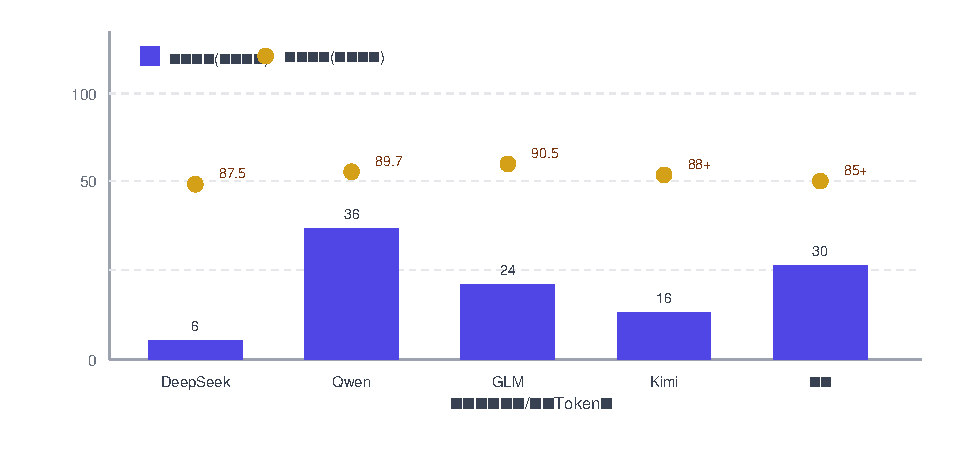
\includegraphics[width=0.92\linewidth]{figures/fig-di-si-shi-er-zhang-1}
\\[2pt]\small 图 4：五款模型的价格与性能对比（价格越低越好，得分越高越好）
\end{center}

\booksection{三、模型选择决策框架}

了解了各模型的特点后，如何为自己的项目选模型？这里送你一套\textbf{“四问决策法”}——回答四个问题，就能锁定最适合你的模型。

你的项目在国内还是国际部署？

国内 选国产模型

|

国际 可选海外模型

核心任务是编程还是其他？

编程 Claude 或 DeepSeek

|

其他 继续判断

需要超长上下文(>50万Token)？

需要 Gemini 或 Kimi

|

不需要 继续判断

预算敏感吗？

敏感 DeepSeek 或 Qwen-turbo

|

不敏感 GPT-5.6 或 Claude

\begin{center}\small\color{gray}图 5：大模型选择四问决策法\end{center}

\begin{tcbinfo}{小贴士：组合策略}
这个决策法不是教条——很多场景需要组合使用多个模型。一个常见的组合策略：用 DeepSeek 或 Qwen 做日常开发（成本低、中文好），用 Claude 做关键架构设计（推理强、幻觉低），用 Gemini 做多模态分析（图像视频处理）。按需切换模型，而不是“一个模型用到死”。

\end{tcbinfo}

\booksection{四、API 调用入门：从零开始接入大模型}

很多 AI 编程教程只教你怎么用对话界面，但真正的“AI 编程”——让你的应用调用大模型——需要通过 API。API（Application Programming Interface，应用程序编程接口）是程序之间的通信协议。通过 API，\textbf{你的代码可以像调用一个函数一样，调用大模型的能力}。

\booksubsection{什么是 Token}

在了解 API 之前，必须先理解 “Token” 这个概念。Token 是大模型计费的基本单位，可以理解为\textbf{“AI 的阅读和写作单位”}。一个 Token 大约对应：英文中 0.75 个单词（4 个字符），中文中 0.5-1 个汉字。一段 1000 字的中文文本，大约消耗 1500-2000 个 Token。

Token 不是字数，也不是字符数。大模型使用专门的分词器（Tokenizer）将文本切分成 Token。同一个词在不同模型中的 Token 数量可能不同——比如“人工智能”在 GPT 中可能是 3 个 Token，在 DeepSeek 中可能是 2 个。大多数模型的 API 会返回实际消耗的 Token 数量，你可以在 API 响应中查看。

\begin{tcbinfo}{Token 成本快速估算}
100 万字中文约等于 150 万 Token。用 DeepSeek V4 Flash 处理 100 万字输入 + 100 万字输出，成本约 0.42 美元（约 3 元人民币）；用 Claude Fable 5 处理同样的量，成本约 60 美元（约 434 元人民币）。\textbf{这就是为什么模型选择直接影响你的项目成本}。

\end{tcbinfo}

\booksubsection{获取 API Key}

使用大模型 API 的第一步是获取 API Key——一串用于身份验证的密钥。每个模型提供商都有自己的 API 平台，你需要注册账号并创建 API Key。以下是主流模型的 API 平台入口和获取流程：

\begin{center}
\begin{tabularx}{\linewidth}{|X|X|X|X|}
\hline
\textbf{模型} & \textbf{API 平台} & \textbf{获取流程} & \textbf{免费额度} \tabularnewline
\hline
DeepSeek & platform.deepseek.com & 注册 实名认证 创建 API Key & 新用户赠送额度 \tabularnewline
通义千问 & bailian.aliyun.com（百炼平台） & 阿里云账号登录 开通服务 创建 Key & 新用户免费试用 \tabularnewline
智谱GLM & open.bigmodel.cn & 注册 实名认证 创建 API Key & 新用户赠送额度 \tabularnewline
Kimi & platform.moonshot.cn & 注册 实名认证 创建 API Key & 有限免费额度 \tabularnewline
豆包 & volcengine.com（火山引擎） & 注册 开通方舟 创建 API Key & 注册送大量 Token \tabularnewline
OpenAI GPT & platform.openai.com & 注册 绑定信用卡 创建 API Key & 无免费额度(需付费) \tabularnewline
Anthropic Claude & console.anthropic.com & 注册 绑卡 创建 API Key & 新用户少量额度 \tabularnewline
\hline
\end{tabularx}
\end{center}

\begin{center}\small\color{gray}主流模型 API 平台及 Key 获取方式（2026 年 8 月）\end{center}

\textbf{安全提示：API Key = 钱包密码}\par

API Key 等同于你的钱包密码——任何拿到 Key 的人都可以用你的额度调用模型。因此：\textbf{永远不要把 API Key 写在代码中}（用环境变量管理）；永远不要把含 Key 的代码提交到公开的 Git 仓库；永远不要在社交媒体分享含 Key 的截图。如果 Key 泄露了，立即在平台上删除并重新创建。

\booksubsection{第一次 API 调用}

获取 API Key 后，你可以用任何编程语言调用大模型 API。以下用 Python 演示一个最简单的调用——向 DeepSeek 发送一条消息并获取回复。

\begin{lstlisting}[language=Python]
# 安装SDK：pip install openai
# DeepSeek兼容OpenAI SDK格式，可以直接用
from openai import OpenAI
import os

# 1. 创建客户端（API Key从环境变量读取）
client = OpenAI(
    api_key=os.environ.get("DEEPSEEK_API_KEY"),
    base_url="https://api.deepseek.com"
)

# 2. 发送请求
response = client.chat.completions.create(
    model="deepseek-chat",  # 指定模型
    messages=[
        {"role": "system", "content": "你是一个Python编程助手。"},
        {"role": "user", "content": "写一个快速排序函数。"}
    ]
)

# 3. 获取回复
print(response.choices[0].message.content)

# 4. 查看Token消耗
print(f"输入Token: {response.usage.prompt_tokens}")
print(f"输出Token: {response.usage.completion_tokens}")
print(f"总Token: {response.usage.total_tokens}")
\end{lstlisting}

这段代码的核心逻辑是：\textbf{创建客户端（携带 API Key 和模型地址） 构造消息列表（system 设定角色，user 是用户输入） 发送请求 获取回复}。这个模式几乎适用于所有兼容 OpenAI 格式的模型——只需要更换 api\_key 和 base\_url 就能切换模型。这就是为什么很多国产模型选择兼容 OpenAI SDK 格式：开发者只需改两行代码就能切换模型，迁移成本极低。

以下是切换到其他模型的代码差异——注意只需要改两行：

\begin{lstlisting}[language=Python]
# DeepSeek
client = OpenAI(
    api_key=os.environ.get("DEEPSEEK_API_KEY"),
    base_url="https://api.deepseek.com"
)
# model="deepseek-chat"

# 通义千问（百炼平台）
client = OpenAI(
    api_key=os.environ.get("DASHSCOPE_API_KEY"),
    base_url="https://dashscope.aliyuncs.com/compatible-mode/v1"
)
# model="qwen-plus"

# 智谱GLM
client = OpenAI(
    api_key=os.environ.get("GLM_API_KEY"),
    base_url="https://open.bigmodel.cn/api/paas/v4"
)
# model="glm-4"

# OpenAI GPT
client = OpenAI(
    api_key=os.environ.get("OPENAI_API_KEY"),
    # base_url使用默认值即可
)
# model="gpt-5.6-terra"
\end{lstlisting}

\booksubsection{流式响应处理}

在实际应用中，你通常不希望等 AI 写完所有内容才一次性显示——那会让用户等太久。流式响应（Streaming）可以让你在 AI 生成的同时逐字显示，大幅提升用户体验。就像打字机一样，字一个一个蹦出来，用户的感觉是完全不同的。

\begin{lstlisting}[language=Python]
# 流式响应：逐字输出
stream = client.chat.completions.create(
    model="deepseek-chat",
    messages=[
        {"role": "user", "content": "写一个Python的冒泡排序教程"}
    ],
    stream=True  # 开启流式响应
)

# 逐块接收并打印
for chunk in stream:
    if chunk.choices[0].delta.content is not None:
        print(chunk.choices[0].delta.content, end="", flush=True)
# 输出会像打字机一样逐字显示
\end{lstlisting}

\booksection{五、Token Plan 购买指南}

大多数模型提供商有两种计费方式：按量计费（Pay-as-you-go）和套餐订阅（Token Plan / Subscription）。理解这两种方式的区别，能帮你大幅降低使用成本。

\booksubsection{按量计费 vs 套餐订阅}

\begin{center}
\begin{tabularx}{\linewidth}{|X|X|X|}
\hline
\textbf{维度} & \textbf{按量计费(Pay-as-you-go)} & \textbf{套餐订阅(Subscription)} \tabularnewline
\hline
计费方式 & 用多少Token付多少钱 & 预付固定费用，获得额度 \tabularnewline
适合场景 & 使用量不稳定、偶尔调用 & 使用量稳定、高频调用 \tabularnewline
价格优势 & 标准价 & 比按量低20\%-50\% \tabularnewline
灵活性 & 随时可用，无需承诺 & 需要预付，额度过期可能作废 \tabularnewline
超额处理 & 自动按量计费 & 超出额度后转为按量计费 \tabularnewline
代表平台 & 各模型官方API平台 & OpenAI Plus/Pro, Claude Pro, Cursor Pro \tabularnewline
\hline
\end{tabularx}
\end{center}

\begin{center}\small\color{gray}两种计费方式的对比\end{center}

对于初学者，建议\textbf{从按量计费开始}——不需要预付费用，用多少花多少。当你的月使用量稳定在一个水平后（比如每月超过 50 元），再考虑切换到套餐订阅以获得更低单价。

\booksubsection{主流订阅套餐一览}

\begin{center}
\begin{tabularx}{\linewidth}{|X|X|X|X|}
\hline
\textbf{套餐} & \textbf{月费} & \textbf{包含内容} & \textbf{适合人群} \tabularnewline
\hline
ChatGPT Free & 免费 & GPT-5.6 Luna 无限文本对话 & 零基础体验 \tabularnewline
ChatGPT Plus & US\$20/月 & GPT-5.6 Sol、图像生成、数据分析、插件访问 & 中度使用者 \tabularnewline
ChatGPT Pro & US\$200/月 & 无限制使用所有模型、优先访问新功能 & 重度专业用户 \tabularnewline
Claude Free & 免费 & 有限次数Claude对话 & 零基础体验 \tabularnewline
Claude Pro & US\$20/月 & 无限制Claude使用、优先访问新模型 & 编程开发者 \tabularnewline
Cursor Free & 免费 & 有限次数AI补全和对话 & 初学者体验 \tabularnewline
Cursor Pro & US\$20/月 & 无限AI补全、500次/月高级请求 & 日常开发者 \tabularnewline
Cursor Business & US\$40/月/人 & 团队协作、管理后台、隐私模式 & 团队使用 \tabularnewline
\hline
\end{tabularx}
\end{center}

\begin{center}\small\color{gray}主流 AI 工具订阅套餐（2026 年 8 月）\end{center}

国内模型的订阅方案略有不同。DeepSeek 主要按量计费，没有月度订阅套餐——你充值后按实际使用量扣费。通义千问在百炼平台提供预付费资源包（购买一定量的 Token 额度，享受折扣价）。豆包在火山引擎上也有类似的预付费方案。对于国内开发者，最经济的组合通常是：\textbf{DeepSeek 按量计费（日常开发）+ 豆包免费额度（体验测试）}。

\booksubsection{API 聚合平台}

如果你需要同时使用多个模型，API 聚合平台是一个省心的选择。聚合平台提供一个统一的 API Key，你就能调用全球几十种模型，无需在每个平台分别注册。

\begin{center}
\begin{tabularx}{\linewidth}{|X|X|X|X|}
\hline
\textbf{平台} & \textbf{特点} & \textbf{价格优势} & \textbf{适合场景} \tabularnewline
\hline
OpenRouter (openrouter.ai) & 海外聚合平台，一个Key调用全球模型 & 价格透明，支持实时比价 & 需要灵活切换多个海外模型 \tabularnewline
SiliconFlow (siliconflow.cn) & 国内聚合平台，提供多种国产模型API & 比官方低20\%-30\% & 国内开发者，多模型比价 \tabularnewline
Azure OpenAI (微软代理) & 微软Azure代理的OpenAI API & Batch API可打5折 & 企业级OpenAI调用，大批量异步任务 \tabularnewline
百度千帆 (qianfan.baidubce.com) & 百度AI云平台，提供文心等模型 & 新用户赠送额度 & 百度生态用户 \tabularnewline
\hline
\end{tabularx}
\end{center}

\begin{center}\small\color{gray}主流 API 聚合平台（2026 年 8 月）\end{center}

\textbf{避坑提醒：别买“共享 Key”}\par

不要在淘宝、闲鱼等平台购买所谓的“共享 API Key”——这些 Key 通常来路不明，可能随时被封号，还有数据泄露风险。始终通过官方平台或正规聚合平台获取 API Key。

\booksubsection{成本优化策略}

选对模型只是第一步，如何“用得省钱”同样重要。以下是几个经过实践验证的成本优化策略：

\begin{enumerate}
  \item \textbf{善用缓存命中}。很多模型提供"缓存"功能——当你的请求中包含之前已经处理过的内容（如系统提示词），这部分只按极低价格计费。DeepSeek 的缓存命中价格仅为普通价格的 1/60。把固定的系统提示放在消息列表开头，可以最大化缓存命中。
  \item \textbf{分级路由}——用便宜模型处理简单任务，贵模型处理复杂任务。比如用 DeepSeek V4 Flash 做文本分类（输出 2 元/百万 Token），用 Claude 做架构设计（输出 181 元/百万 Token）。一个项目里 80\% 的调用可以用便宜模型。
  \item \textbf{限制输出长度}。API 按输出 Token 计费，输出越长越贵。在不需要长篇大论的场景中，设置 max\_tokens 参数限制输出长度，避免 AI"废话太多"。
  \item \textbf{使用 Batch API 处理非实时任务}。如果你有大量不需要即时响应的任务（如批量数据标注、文档摘要），使用 Batch API 可以享受 50\% 折扣。OpenAI 和 Azure 都提供这个功能。
  \item \textbf{监控 Token 用量}。大多数 API 平台提供用量统计面板。定期查看用量分布，找出消耗 Token 最多的调用，针对性优化。一个小小的 Prompt 调整（比如把"请详细解释"改成"请用 3 句话解释"）可能节省 50\% 的 Token。
\end{enumerate}

\begin{center}
\begin{tabularx}{\linewidth}{|X|X|X|X|}
\hline
\textbf{优化策略} & \textbf{节省幅度} & \textbf{实施难度} & \textbf{说明} \tabularnewline
\hline
缓存命中 & 最高98\% & 低 & 把固定内容放在消息开头 \tabularnewline
分级路由 & 50\%-80\% & 中 & 简单任务用便宜模型 \tabularnewline
限制输出长度 & 30\%-60\% & 低 & 设置max\_tokens参数 \tabularnewline
Batch API & 50\% & 低 & 非实时任务用批处理 \tabularnewline
Prompt优化 & 20\%-50\% & 中 & 精简Prompt，减少冗余 \tabularnewline
\hline
\end{tabularx}
\end{center}

\begin{center}\small\color{gray}成本优化策略及效果（2026 年 8 月）\end{center}

\booksection{六、实战：在项目中接入大模型 API}

让我们用一个完整的实战来结束本章——创建一个\textbf{“AI 摘要生成器”}：用户输入一段长文本，调用大模型 API 生成摘要。这个实战会展示 API 调用的完整流程：环境配置、API 调用、错误处理、成本控制。

\begin{lstlisting}[language=Python]
# ai_summarizer.py - AI摘要生成器
import os
from openai import OpenAI

# 1. 配置（API Key从环境变量读取，绝不硬编码）
client = OpenAI(
    api_key=os.environ.get("DEEPSEEK_API_KEY"),
    base_url="https://api.deepseek.com"
)

def summarize(text: str, max_length: int = 200) -> dict:
    """生成文本摘要

    Args:
        text: 要摘要的原文
        max_length: 摘要最大长度（Token数）

    Returns:
        dict: 包含摘要和Token消耗信息
    """
    try:
        response = client.chat.completions.create(
            model="deepseek-chat",
            messages=[
                {
                    "role": "system",
                    "content": "你是一个摘要生成器。"
                               "请用简洁的中文总结用户提供的文本。"
                               "摘要不超过3句话。"
                },
                {
                    "role": "user",
                    "content": f"请摘要以下文本:\n\n{text}"
                }
            ],
            max_tokens=max_length,  # 限制输出长度
            temperature=0.3  # 低温度=更稳定
        )

        return {
            "success": True,
            "summary": response.choices[0].message.content,
            "input_tokens": response.usage.prompt_tokens,
            "output_tokens": response.usage.completion_tokens,
            "total_tokens": response.usage.total_tokens
        }

    except Exception as e:
        return {
            "success": False,
            "error": str(e)
        }

# 2. 使用示例
if __name__ == "__main__":
    long_text = """
    （粘贴一段长文本...）
    """

    result = summarize(long_text)

    if result["success"]:
        print(f"摘要: {result['summary']}")
        print(f"消耗Token: {result['total_tokens']}")
        # 估算成本：DeepSeek V4 Flash
        cost = result['total_tokens'] * 0.000004  # 约0.4分/千Token
        print(f"预估成本: {cost:.4f}元")
    else:
        print(f"出错了: {result['error']}")
\end{lstlisting}

这段代码体现了 API 调用的几个最佳实践：API Key 通过环境变量读取，绝不硬编码在代码中；函数有清晰的文档和类型提示；设置了 max\_tokens 限制输出长度；temperature 设为低值（0.3）以获得更稳定的输出；有完整的错误处理；返回 Token 消耗信息用于成本追踪。当你用 AI 来写这段代码时，可以告诉它这些要求——它完全有能力帮你实现。

本章的最终启示：模型是"弹药"，方法论是"战术"。选对弹药能让战斗更顺利，但没有好的战术，再好的弹药也打不赢仗。了解了各模型的特点和 API 使用方法后，你就有了一个充足的"弹药库"——但怎么打这场仗，还是要靠前几章学到的思维方法论。

\begin{tcbpractice}{来动手：跑通你的第一次 API 调用}
注册一个国产模型平台（推荐 DeepSeek 或智谱，都送新用户额度），创建 API Key，把它写进系统环境变量（而不是代码里！），然后运行上面“第一次 API 调用”的代码。看到 AI 的回复打印出来的那一刻，你就跨过了“用 AI”和“造 AI 应用”之间的分界线。

\end{tcbpractice}

\begin{tcbsummary}{本章小结}
\begin{itemize}
  \item 国际三强：GPT-5.6（均衡全能）、Claude（编程天花板+幻觉率仅1\%）、Gemini（多模态之王+200万上下文）
  \item 国产五强：DeepSeek V4（性价比之王，注意涨价公告）、Qwen3.7（企业级）、GLM-5.1（SWE国产第一）、Kimi K3（超长文本）、豆包（免费入门）
  \item 四问决策法：部署地点？编程还是其他？超长上下文？预算敏感？
  \item Token 是计费单位：中文 1 字约 1.5-2 Token；100万字约150万Token
  \item API Key = 钱包密码：环境变量管理，绝不硬编码、不上传Git
  \item 国产模型普遍兼容 OpenAI SDK：换模型只需改 api\_key 和 base\_url 两行
  \item 省钱五招：缓存命中、分级路由、限制输出、Batch API、监控用量
\end{itemize}

\end{tcbsummary}

\bookchapter{第四十三章：对话工程——与AI高效协作的对话技术}

\chapterintro{对话是 AI 编程的核心交互方式。但请注意：“对话”不等于“聊天”——高效的 AI 编程对话是一种有结构的沟通技术，我们称之为“对话工程”。它研究的是：如何用最少的对话轮次，获得最高质量的代码产出。说白了，这一章就是教你怎么和 AI“把话说清楚”。}

\booksection{一、Prompt 分层策略}

与 AI 的对话可以分为三个层次，每层承担不同的功能。理解这三个层次，你就能像搭积木一样组合出高效的 Prompt。

\begin{center}
\begin{tabularx}{\linewidth}{|X|X|X|X|}
\hline
\textbf{层次} & \textbf{功能} & \textbf{示例} & \textbf{频率} \tabularnewline
\hline
系统层 & 设定AI的角色和全局约束 & "你是一个React专家，代码必须用TypeScript" & 项目开始时设置一次 \tabularnewline
任务层 & 描述当前要做的具体任务 & "实现一个表单组件，包含用户名和密码字段" & 每个任务开始时给出 \tabularnewline
反馈层 & 对AI产出进行评价和修正 & "密码字段缺少显示/隐藏切换，请添加" & 根据产出质量给出 \tabularnewline
\hline
\end{tabularx}
\end{center}

\begin{center}\small\color{gray}对话 Prompt 的三个层次\end{center}

系统层的 Prompt 通常写在项目记忆文件中（如 CLAUDE.md），不需要每次对话重复。任务层是你在对话中最常使用的——它应该包含\textbf{“做什么”“用什么技术”“有什么约束”}三个要素。反馈层是最考验功力的——好的反馈能让 AI 精准修正，坏的反馈只会让它重新猜测。

\begin{tcbinfo}{小贴士：反馈三板斧}
一个实用的反馈模板是“指出问题 + 说明期望 + 提供上下文”。比如：“第 25 行的错误处理只用了 console.log（指出问题），生产环境应该用统一的错误处理器并返回用户友好提示（说明期望），项目里有一个 handleError 函数可以用（提供上下文）”。这种反馈比“改一下错误处理”有效十倍。

\end{tcbinfo}

\booksection{二、调试对话：如何描述错误让 AI 快速定位}

调试是 AI 编程中最频繁的场景之一。当你遇到 bug 时，如何向 AI 描述问题，直接决定了它能否快速帮你定位和修复。以下是调试对话的四个要点：

\begin{enumerate}
  \item \textbf{给 AI"看"原始信息，而不是你的转述}。把错误日志、异常堆栈、相关代码直接 @ 引用给 AI，而不是用"好像有个什么报错"来描述。AI 看到原始信息比看到你的理解更准确。
  \item \textbf{描述"期望行为"和"实际行为"的差异}。"我期望点击按钮后跳转到首页（期望），但实际点击后页面没有反应（实际）"——这种描述比"按钮坏了"有用得多。
  \item \textbf{提供复现步骤}。"先输入用户名，然后点击登录按钮，就会出现这个错误"——复现步骤让 AI 能模拟你的操作路径，更容易定位问题。
  \item \textbf{说清楚你已经尝试了什么}。"我已经检查了网络请求，返回 200，数据正常"——这能帮 AI 排除已验证的方向，不浪费时间重复排查。
\end{enumerate}

差的调试描述

\begin{lstlisting}
按钮点击没反应，帮我看看
\end{lstlisting}

好的调试描述

\begin{lstlisting}
点击登录按钮后页面无反应。
期望行为：点击后跳转到 /home 页面
实际行为：点击后无任何反应，控制台无报错
复现步骤：
1. 在登录页输入用户名admin和密码123456
2. 点击"登录"按钮
3. 页面无反应
已排查：
- 网络请求正常，返回200
- onClick事件已绑定
- 检查了LoginButton组件的代码
相关文件：@src/components/LoginButton.tsx
@src/pages/Login.tsx
\end{lstlisting}

\booksection{三、迭代策略：小步快跑 vs 大步重构}

AI 编程中的迭代有两种基本策略，适用于不同场景。理解它们的区别，能帮你在不同情况下做出正确选择。

\textbf{“小步快跑”}策略适用于功能开发和 bug 修复。它的核心是：每次让 AI 只做一个小的修改，验证通过后再做下一个。优势是每一步都可验证、可回退，风险可控；劣势是速度较慢，需要频繁的对话交互。适合：新功能开发、不确定最优方案时的探索、对 AI 产出不太放心时的谨慎迭代。

\textbf{“大步重构”}策略适用于明确知道目标的大规模修改。它的核心是：一次性描述完整的目标，让 AI 自主规划和执行整个修改。优势是速度快，AI 能看到全局图景做出更优的架构决策；劣势是风险高，如果 AI 理解偏差，修正成本大。适合：明确的架构升级、大规模代码迁移、有充分测试保障的重构。

\begin{center}
\begin{tabularx}{\linewidth}{|X|X|X|}
\hline
\textbf{维度} & \textbf{小步快跑} & \textbf{大步重构} \tabularnewline
\hline
每次修改量 & 一个功能点或一个bug & 一个模块或一个架构层 \tabularnewline
验证频率 & 每次修改后立即验证 & 全部修改完成后统一验证 \tabularnewline
对话轮次 & 多（5-10轮/功能） & 少（1-3轮/模块） \tabularnewline
风险 & 低，每步可回退 & 高，偏差修正成本大 \tabularnewline
适用场景 & 新功能、探索性开发 & 明确目标的重构、迁移 \tabularnewline
前提条件 & 无特殊要求 & 需要有测试覆盖 \tabularnewline
\hline
\end{tabularx}
\end{center}

\begin{center}\small\color{gray}两种迭代策略的对比\end{center}

实践中，两种策略常常组合使用。比如重构一个模块时，先用“大步重构”让 AI 给出整体方案，审查方案后，再用“小步快跑”逐步执行。这样既保证了全局视角，又控制了执行风险。

\booksection{四、多轮对话的上下文管理}

随着对话轮次增加，你需要主动管理对话上下文，避免“AI 忘记了早期信息”的问题。以下是几个实用的上下文管理技巧。

\textbf{第一，“锚定”关键信息。}在对话开始时，把关键约束写清楚，并在后续对话中适时重申。比如“记住，我们的数据存在 localStorage，不能用数据库”——在相关的修改请求中重申这个约束，防止 AI 遗忘。

\textbf{第二，善用“总结-续接”技巧。}当对话变得很长时，可以让 AI“总结一下目前的进展和待办事项”，然后开一个新对话，把这个总结作为起点。这样既保留了关键上下文，又避免了长对话的退化。

\textbf{第三，“一个对话一个任务”。}这是最简单也最有效的上下文管理策略。每个对话只处理一个任务或一个功能点，完成后开新对话处理下一个。这天然限制了对话长度，保持上下文清晰。

\textbf{第四，利用工具的上下文管理功能。}大多数 AI 编程工具都有“清除上下文”或“新会话”按钮——当你感觉 AI 的回答质量下降时，不要犹豫，开一个新会话。丢失一些对话历史比继续在退化的上下文中挣扎要好得多。

\begin{tcbpractice}{来动手：给你的 AI 当一次"病人"}
故意在浏览器里做一个小页面，制造一个 bug（比如按钮没反应）。然后按本章“好的调试描述”的格式，向 AI 完整描述一次：原始信息、期望 vs 实际、复现步骤、已排查项。感受一下 AI 定位问题的速度差异——你会理解为什么“描述问题”本身是门手艺。

\end{tcbpractice}

\begin{tcbsummary}{本章小结}
\begin{itemize}
  \item Prompt 三层：系统层（写在记忆文件）、任务层（做什么+技术+约束）、反馈层（指出问题+期望+上下文）
  \item 调试四要点：给原始信息、期望vs实际、复现步骤、已排查项
  \item 小步快跑：低风险高轮次，适合新功能；大步重构：高风险低轮次，需要测试保障
  \item 上下文管理四招：锚定关键信息、总结-续接、一个对话一个任务、果断开新会话
\end{itemize}

\end{tcbsummary}

\bookchapter{第四十四章：从0到1实战——完整项目全流程}

\chapterintro{理论学完了，现在是动手的时候。本章不是简单的“照着敲”教程，而是一套“怎么想、怎么问、怎么验”的实战方法论。我们会用三个不同难度的项目，展示从需求到成品的完整思考过程。无论你用哪个工具，这套流程都适用。}

\booksection{一、项目一：极简个人工具站（入门级）}

\booksubsection{需求思考}

目标：创建一个个人工具站网页，展示 3-4 个实用小工具的入口。这是一个纯前端项目，不需要后端和数据库。重点不是工具本身有多复杂，而是体验“从需求到成品”的完整流程。

按照需求五要素：Who——个人使用。What——一个展示工具入口的网页。Why——把常用工具集中在一个页面方便访问。How——单文件 HTML+CSS+JS，不使用框架。Constraint——30 分钟内完成，不需要部署。

\booksubsection{下达指令}

基于 Think Before Coding 原则，你的指令应该包含足够的信息让 AI 理解目标，但不需要指定每个实现细节：

\begin{lstlisting}
请创建一个个人工具站网页，要求：
1. 单文件HTML（内联CSS和JS），不使用框架
2. 暗色主题，现代极简风格
3. 展示4个工具入口卡片：
   - 文本摘要工具
   - 字数统计工具
   - 颜色选择器
   - 二维码生成器
4. 每个卡片有图标、标题、简短描述
5. 卡片有悬停动画效果
6. 响应式布局，手机上可用
7. 顶部有一个标题栏
请直接给出完整的HTML文件。
\end{lstlisting}

\booksubsection{验收与迭代}

AI 给出代码后，按照迭代验证的三层检查进行验收。第一层功能验证：文件能否在浏览器中打开？4 个卡片是否都显示了？悬停动画是否正常？第二层边界验证：在手机屏幕尺寸下布局是否正常？窗口很窄时卡片是否会换行？第三层架构验证：代码是否可读？CSS 是否内联在一个 style 标签中？有没有明显的冗余？

如果某个工具卡片的功能也想实现（而不只是入口），可以逐步添加——每次添加一个工具的功能，验证后再添加下一个。这就是“小步快跑”策略的实际应用。

\booksection{二、项目二：全栈记账系统（进阶级）}

\booksubsection{需求思考与 PRD}

目标：一个有前端、后端和数据库的全栈记账应用。这个项目比第一个复杂得多，需要用到第四十章的需求工程方法。

先写 PRD。按照第四十章第三节的模板，写出项目概述、功能列表、技术方案、数据模型和开发计划。技术方案的选择要考虑 Simplicity First 原则——前端用 React 但不引入 Redux 等复杂状态管理，后端用 Node.js 但不引入微服务，数据库用 SQLite 而非 PostgreSQL（开发阶段）。

开发计划拆解为 5 步：Step 1 后端 API 骨架（Express 服务器 + SQLite + CRUD 接口）；Step 2 前端基础页面（记录列表 + 添加表单）；Step 3 前后端联调（API 调用 + 数据展示）；Step 4 分类和筛选功能；Step 5 月度汇总和简单图表。\textbf{每步完成后都是“能用的东西”}。

\booksubsection{设置项目记忆文件}

在开始编码之前，先创建项目记忆文件。这是上下文工程的核心实践——让 AI 在每次对话开始时都了解项目背景。

\begin{lstlisting}
# 项目：全栈记账应用
## 概述
个人记账应用，支持收支记录、分类、月度汇总。
## 技术栈
- 前端：React + TypeScript + Vite
- 后端：Node.js + Express + TypeScript
- 数据库：SQLite (通过 better-sqlite3)
- 前后端共享类型定义
## API约定
- 基础路径：/api
- 返回格式：{ success: boolean, data: any, error: string }
- RESTful风格
## 数据模型
Record { id, amount, type, category, note, date }
## 代码规范
- TypeScript严格模式
- 缩进2空格
- 函数有JSDoc注释
- 中文注释和提交信息
\end{lstlisting}

\booksubsection{逐步实现}

按照开发计划，每一步用一个独立的对话来完成。以下是第一步的指令示例：

\begin{lstlisting}
我需要创建后端API骨架。
要求：
1. Express服务器，端口3001
2. SQLite数据库，表名records
3. records表字段：
   id (TEXT PRIMARY KEY)
   amount (REAL)
   type (TEXT: 'income'|'expense')
   category (TEXT)
   note (TEXT)
   date (TEXT: YYYY-MM-DD)
4. CRUD接口：
   GET /api/records - 获取所有记录
   POST /api/records - 新增记录
   PUT /api/records/:id - 更新记录
   DELETE /api/records/:id - 删除记录
5. 错误处理中间件
请给出完整的后端代码结构。
\end{lstlisting}

注意这个指令的特点：它\textbf{只描述当前这一步}（后端骨架），不掺杂前端需求；它\textbf{明确列出了字段和接口}（给 AI 足够的约束），但具体实现由 AI 决定；它遵循了 Goal-Driven Execution 原则——说“做什么”而非“怎么做”。

AI 给出代码后，立即验证：运行服务器，用 curl 或 Postman 测试每个接口是否正常工作。确认无误后，开新对话处理 Step 2（前端基础页面）。每一步都遵循“指令-验证-新对话”的循环。

\booksection{三、项目三：AI 增强应用（高级）}

\booksubsection{项目构思}

目标：一个接入大模型 API 的应用——比如一个“AI 学习助手”，用户输入学习内容，AI 生成摘要、关联知识点、推荐学习资源。这个项目的特殊之处在于：\textbf{你的应用本身就在调用 AI}，你需要处理 API 调用、prompt 工程、错误处理等新问题。

这个项目教会你的最重要的一课是：当你“用 AI 来写调用 AI 的代码”时，你需要格外注意 prompt 工程。你的应用调用大模型 API 时使用的 prompt，也需要遵循本指南讨论的原则——清晰、简洁、目标驱动。

\booksubsection{关键技术点}

这个项目涉及几个你在前两个项目中没遇到的技术点：

\begin{itemize}
  \item \textbf{API 密钥管理}：密钥绝不能硬编码在代码中，用环境变量管理；
  \item \textbf{流式响应处理}：大模型的回复通常是流式的，需要逐字显示；
  \item \textbf{Token 用量控制}：大模型按 token 计费，需要在应用层面控制用量；
  \item \textbf{Prompt 模板管理}：不同功能用不同的 prompt 模板，需要结构化管理。
\end{itemize}

这些技术点都可以让 AI 帮你实现，但你需要理解每个技术点的“为什么”——为什么密钥不能硬编码？为什么需要流式响应？为什么 token 用量需要控制？\textbf{理解了“为什么”，你才能判断 AI 的方案是否合理}。

\booksection{四、通用实战流程清单}

无论项目大小，以下是一个通用的 AI 编程实战流程清单。每次开始新项目时，过一遍这个清单，确保没有遗漏关键步骤。

\begin{center}
\begin{tabularx}{\linewidth}{|X|X|X|}
\hline
\textbf{阶段} & \textbf{做什么} & \textbf{对应原则} \tabularnewline
\hline
1. 需求思考 & 过一遍需求五要素，想清楚要做什么 & Think Before Coding \tabularnewline
2. 需求拆解 & 把大需求拆成可独立验证的小步骤 & Simplicity First \tabularnewline
3. 写PRD & 整理成结构化文档，作为参考 & Goal-Driven \tabularnewline
4. 设置记忆文件 & 创建CLAUDE.md或同类文件 & Harness Engineering \tabularnewline
5. 逐步实现 & 每步一个对话，指令-验证-下一步 & Surgical Changes \tabularnewline
6. 测试验证 & 每步完成后立即测试功能正确性 & Iterate \& Verify \tabularnewline
7. 代码审查 & 检查架构合理性、安全性、可维护性 & Iterate \& Verify \tabularnewline
8. 迭代优化 & 根据测试和审查结果迭代改进 & Iterate \& Verify \tabularnewline
\hline
\end{tabularx}
\end{center}

\begin{center}\small\color{gray}AI 编程通用实战流程清单\end{center}

\begin{tcbpractice}{来动手：本周完成"项目一"}
把第四十四章第一节的“个人工具站”当成你的第一个 AI 编程作业：花 5 分钟过五要素，把指令发给 AI（任何工具都行），再按三层验证验收。30 分钟内完成它——你的第一个 AI 编程作品就诞生了。做完记得把它存好，这是你从“读者”变成“实践者”的纪念品。

\end{tcbpractice}

\begin{tcbsummary}{本章小结}
\begin{itemize}
  \item 项目一（入门）：纯前端工具站——体验完整流程，30 分钟能完成
  \item 项目二（进阶）：全栈记账系统——PRD + 记忆文件 + 5 步逐步实现，每步"能用"
  \item 项目三（高级）：AI 学习助手——用 AI 写调用 AI 的代码，注意 prompt 工程
  \item 通用流程八步：需求思考拆解PRD记忆文件逐步实现测试审查迭代
  \item 每一步都遵循"指令-验证-新对话"循环
\end{itemize}

\end{tcbsummary}

\bookchapter{第四十五章：质量保障——让AI写的代码可靠}

\chapterintro{AI 写的代码有一个特点：它通常“看起来很对”——变量命名规范、注释齐全、逻辑清晰。但“看起来对”不等于“真的对”。AI 代码中隐藏的问题往往比手写代码更难发现，因为它的表面质量太高了，容易让人放松警惕。本章教你如何为 AI 代码建立有效的质量保障体系——用测试、审查、版本控制三道防线，把“看起来对”变成“真的对”。}

\booksection{一、测试驱动：让 AI 写测试}

测试是 AI 编程质量保障的第一道防线。好消息是：\textbf{让 AI 写测试比让它写功能代码更容易、更可靠}——因为测试的预期行为是明确的，不太容易产生“看起来对但实际不对”的代码。

测试驱动的 AI 编程流程是：先让 AI 写功能代码，验证基本功能通过后，立即让它写测试用例。测试用例应覆盖正常路径、边界情况和异常情况。然后再让 AI 根据测试反馈修正功能代码。这个流程的好处是：测试一旦写好，就是持续的验证工具——后续任何修改都可以通过运行测试来确认没有引入回归问题。

\begin{lstlisting}
请为 calculate_discount 函数编写单元测试。
测试用例应覆盖：
1. 正常路径：
   - 100元商品打8折 -> 80
   - 200元商品打5折 -> 100
2. 边界情况：
   - 0元商品打8折 -> 0
   - 100元商品打0折 -> 100（不打折）
   - 100元商品打10折 -> 100（全价）
3. 异常情况：
   - 负数价格 -> 应抛出错误
   - 折扣率 > 1 -> 应抛出错误
   - 非数字输入 -> 应抛出错误
使用Vitest框架，给出完整测试文件。
\end{lstlisting}

注意这个指令的特点：它\textbf{明确列出了三类测试用例}（正常、边界、异常），不给 AI 自由发挥的空间去“选择性测试”。AI 有时候会只写正常路径的测试来“快速交差”，明确列出所有类别可以避免这个问题。

\booksection{二、代码审查技巧}

即使有测试覆盖，你仍然需要对 AI 产出的代码进行人工审查。代码审查不是逐行阅读——那太耗时也太依赖你的编程水平。有效的 AI 代码审查应该关注以下几个关键维度：

\begin{center}
\begin{tabularx}{\linewidth}{|X|X|X|}
\hline
\textbf{审查维度} & \textbf{关注什么} & \textbf{常见问题} \tabularnewline
\hline
安全性 & 输入验证、密钥处理、SQL注入防护 & AI经常忘记验证输入，密钥硬编码在代码中 \tabularnewline
错误处理 & 异常是否被捕获，错误信息是否合理 & AI喜欢用空catch块或只console.log \tabularnewline
性能 & 是否有明显的性能问题，如N+1查询、无限循环 & AI有时会写出O(n²)的算法 \tabularnewline
可维护性 & 代码结构是否清晰，命名是否有意义 & AI偶尔会生成过度抽象的代码 \tabularnewline
依赖管理 & 引入的依赖是否必要，版本是否明确 & AI倾向于引入不必要的库 \tabularnewline
\hline
\end{tabularx}
\end{center}

\begin{center}\small\color{gray}AI 代码审查的关键维度\end{center}

审查时不必自己逐一检查——可以让 AI 帮你做第一轮审查。指令如：“请审查这段代码的安全性、错误处理和性能，指出潜在问题。”AI 的自我审查能力在不断提升，虽然不能完全替代人工审查，但能帮你过滤掉大部分明显问题。

\booksection{三、版本控制：Git 在 AI 编程中的角色}

Git 在 AI 编程中的角色比在传统编程中更加重要。因为 AI 的每次修改都可能引入不可预知的变化，你需要一个可靠的“后悔药”——\textbf{版本控制就是那个后悔药}。

AI 编程中 Git 的最佳实践是“频繁提交、小步快进”。每完成一个可验证的功能点，就提交一次。这样当 AI 的某次修改出了问题时，你可以精准回退到上一个可用状态，而不需要推翻所有工作。

另一个实用技巧是“分支隔离”。对于不确定结果的 AI 修改（比如大步重构），先创建一个新分支来做。如果结果满意，合并回主分支；如果不满意，直接删除分支，不影响主分支。这比在主分支上反复修改安全得多。

\begin{enumerate}
  \item 每次 AI 修改前，确保工作区是干净的（没有未提交的更改）。这样如果 AI 的修改不满意，可以用\texttt{git checkout .}快速回退。
  \item 每次 AI 修改后、验证通过后，立即提交。提交信息描述这次修改做了什么，比如"feat: 添加用户注册功能"。
  \item 对于大步重构，先创建分支：\texttt{git checkout -b refactor/auth-system}。在分支上完成修改，测试通过后再合并。
  \item 养成查看 diff 的习惯。每次 AI 修改后，用\texttt{git diff}查看具体改了什么。这不仅能帮你发现问题，还能帮你学习代码。
\end{enumerate}

\booksection{四、常见陷阱与避坑指南}

AI 编程中有几个反复出现的陷阱，几乎所有初学者都会踩。提前知道它们，能帮你少走很多弯路。

\booksubsection{陷阱一：信任陷阱}

“AI 写的代码看起来很专业，一定没问题吧？”——这是最危险的陷阱。AI 生成的代码在表面上非常整洁——命名规范、注释齐全、结构清晰——这种“表面专业感”会让人放松警惕。但\textbf{表面整洁不代表逻辑正确}。\textbf{解药}：永远通过测试验证，而非通过“看起来对不对”判断。

\booksubsection{陷阱二：膨胀陷阱}

“既然 AI 能帮我写代码，那不如把功能做得全面一点？”——这会导致代码膨胀。AI 很擅长“多给”：你让它做一个登录页面，它会给你一套完整的用户管理系统。多余的功能不仅增加复杂度，还增加了出 bug 的概率。\textbf{解药}：严格遵循 Simplicity First 原则，明确告诉 AI“只做这个功能，不要额外添加”。

\booksubsection{陷阱三：理解陷阱}

“AI 应该理解我的意思吧？”——不一定。AI 的理解能力虽然很强，但对模糊的需求仍然会“猜”。当它猜错了，产出的代码就是错的。更麻烦的是，它猜错的代码通常“看起来很合理”，让你误以为它理解了。\textbf{解药}：在指令中提供足够的具体细节，减少 AI 需要“猜”的空间。

\booksubsection{陷阱四：上下文陷阱}

“我在之前的对话里说过了，AI 应该还记得吧？”——很可能不记得。随着对话变长或开新会话，AI 会丢失早期上下文。如果某个关键约束没有被写入项目记忆文件，它很可能在后续修改中被忽略。\textbf{解药}：关键约束写入项目记忆文件，不要依赖对话记忆。

\begin{tcbwarn}{四大陷阱速记}
信任陷阱——别信“看起来对”；膨胀陷阱——AI 爱“多给”；理解陷阱——模糊需求它会“猜”；上下文陷阱——对话记忆会“忘”。对应的解药分别是：测试验证、砍掉多余、给足细节、写入记忆文件。

\end{tcbwarn}

\begin{tcbpractice}{来动手：给你的项目建三道防线}
如果你已经开始做项目一（工具站）：(1) 让 AI 给核心函数写 3 类测试用例；(2) 按五个维度审查一遍代码（安全性/错误处理/性能/可维护性/依赖）；(3) 用 git 初始化项目，做第一次提交。三道防线齐了，你的项目才真正属于你。

\end{tcbpractice}

\begin{tcbsummary}{本章小结}
\begin{itemize}
  \item AI 代码"看起来对"$\neq$"真的对"——表面质量太高反而容易放松警惕
  \item 让 AI 写测试：明确列出正常/边界/异常三类用例，防止"选择性测试"
  \item 审查五维度：安全性、错误处理、性能、可维护性、依赖管理
  \item Git 是"后悔药"：频繁提交、小步快进、分支隔离、常看 diff
  \item 四大陷阱：信任（测试验证）、膨胀（砍掉多余）、理解（给足细节）、上下文（写入记忆文件）
\end{itemize}

\end{tcbsummary}

\bookchapter{第四十六章：进阶之路——从使用者到架构师}

\chapterintro{当你掌握了第三十七至四十四章的方法论，能熟练地用 AI 完成项目开发后，下一步是什么？本章探讨从“AI 工具使用者”到“AI 系统架构师”的进阶之路。这个阶段的关注点不再是“怎么让 AI 写好代码”，而是“怎么让 AI 更好地融入整个开发流程”。}

\booksection{一、MCP 协议与工具扩展}

\textbf{MCP（Model Context Protocol）}是 2025 年出现、2026 年逐渐普及的一个开放协议，它定义了 AI 模型与外部工具之间的通信标准。简单来说，MCP 让 AI 能够“使用工具”——不只生成代码，还能执行命令、查询数据库、调用 API、操作文件系统。

在 MCP 之前，每个 AI 工具都有自己的工具集成方式，互不兼容。MCP 的出现意味着：\textbf{一个符合 MCP 标准的工具可以被任何支持 MCP 的 AI 工具使用}。这大大降低了工具集成的成本，也让 AI 的能力边界从“生成文本”扩展到了“执行动作”。

对于进阶用户来说，MCP 的意义在于：你可以为 AI 构建定制化的工具能力。比如，如果你的团队有一套内部的部署系统，你可以写一个 MCP 工具让 AI 直接调用部署系统，而不需要人工切换到终端操作。这种“AI 调用工具”的能力，是 Agentic Engineering 的基础设施。

\booksection{二、自定义工作流与 Skills}

当你反复执行某些固定的 AI 编程流程时，可以把它们固化成“自定义工作流”或“Skills”。比如，你的团队可能有一套标准的代码审查流程——先检查安全性，再检查性能，再检查可维护性。你可以把这个流程写成一个 Skill，让 AI 在每次代码审查时自动按这个流程执行。

自定义工作流的核心价值是“\textbf{一致性}”——它确保每次执行都遵循同样的标准，不会因为对话长短或上下文不同而产生偏差。这对于团队协作尤其重要：每个成员使用同样的工作流，产出的代码风格和质量标准就会趋于一致。

构建自定义工作流的方法因工具而异。Cursor 支持 Rules 和 Custom Instructions，Claude Code 支持自定义命令，Replit 支持 Runme。但核心思路一样：\textbf{把你的最佳实践“编码”成 AI 可执行的指令模板}。

\booksection{三、多 Agent 协作模式}

到 2026 年，多 Agent 协作开始成为一个热门话题。它的核心理念是：不只用一个 AI 来完成任务，而是用多个分工不同的 AI 来协作。比如，一个 AI 负责写代码，一个 AI 负责写测试，一个 AI 负责代码审查——它们各司其职，互相检查。

多 Agent 协作的优势在于“分工”和“交叉验证”：每个 Agent 专注于自己的领域，产出质量更高；Agent 之间的交叉检查可以发现自己可能忽略的问题。但劣势也很明显：协调成本高，通信开销大，调试更复杂。

\begin{tcbinfo}{小贴士：一个人也能玩"多 Agent"}
对于个人开发者来说，你不需要搭建复杂的多 Agent 系统——你可以“扮演”不同的角色来模拟多 Agent 协作。比如：先用一个对话让 AI 写功能代码；然后开一个新对话（提供 CLAUDE.md 上下文），让 AI“作为代码审查者审查这段代码”；最后再开一个对话让 AI“根据审查意见修正代码”。这种“一人多角”的方式，能获得多 Agent 协作的大部分好处，而不需要复杂的基础设施。

\end{tcbinfo}

\booksection{四、持续学习路径}

AI 编程是一个快速变化的领域。今天的最佳实践，明天可能就需要更新。以下是几条持续学习的建议：

\textbf{第一，关注源头而非二手解读。}Andrej Karpathy 的原始推文和 CLAUDE.md、Anthropic 和 OpenAI 的官方文档、各大工具的更新日志——这些是第一手信息。社区文章和教程是对这些信息的解读和总结，有价值但可能失真。养成读原始资料的习惯。

\textbf{第二，实践驱动学习。}不要“学完再做”，而要“边做边学”。每次遇到新的问题类型（比如第一次处理文件上传、第一次接入第三方 API），就以此为机会学习相关知识。实践中的学习效率远高于脱离场景的理论学习。

\textbf{第三，保持工具敏感度但不过度追新。}每隔一两个月，花半天时间了解最新的工具和趋势——但不要每次有新工具就切换。判断标准是：新工具是否能显著提升你的某个瓶颈？如果不能，当前的组合就够了。

\textbf{第四，构建个人知识库。}把你每次解决复杂问题的对话、每次踩坑的教训、每次有效的方法记录下来。不需要公开发布——这是你自己的“方法论笔记”。随着时间积累，它会成为你最宝贵的资产。

\begin{tcbpractice}{来动手：开一个"踩坑笔记本"}
今天就建一个文档（笔记软件或 .md 文件都行），写下你到目前为止最想记住的三条 AI 编程心得——哪怕是“记得先想清楚再问”。以后每次踩坑、每次学到新招，都往里面记一条。半年后回看，你会感谢今天的自己。

\end{tcbpractice}

\begin{tcbsummary}{本章小结}
\begin{itemize}
  \item MCP 是 AI 与工具之间的通信标准：让 AI 能执行命令、查数据库、调 API
  \item 自定义工作流/Skills 的核心价值是"一致性"：把最佳实践编码成指令模板
  \item 多 Agent = 分工 + 交叉验证；个人开发者可用"一人多角"模拟
  \item 持续学习四招：读源头、边做边学、不过度追新、建个人知识库
\end{itemize}

\end{tcbsummary}

\bookchapter{第四十七章：速查手册与资源}

\chapterintro{本章是一份可以独立使用的速查手册。当你记不清某个原则或需要快速决策时，直接翻到这里。建议你把它当成“口袋卡片”：五大原则速查、工具决策树、常见问题、学习资源，一页不落。}

\booksection{一、思维模型速查卡}

\begin{center}
\begin{tabularx}{\linewidth}{|X|X|X|}
\hline
\textbf{原则} & \textbf{一句话} & \textbf{操作要点} \tabularnewline
\hline
Think Before Coding & 先想清楚再开口 & 回答三问：做什么？结果长啥样？有什么约束？ \tabularnewline
Simplicity First & 用最少代码解决问题 & 每次只做一个功能，砍掉不必要的复杂度 \tabularnewline
Surgical Changes & 精准修改不越界 & 明确指定修改范围，拒绝AI的"顺手改一下" \tabularnewline
Goal-Driven Execution & 说"做什么"不说"怎么做" & 给目标不给步骤，让AI自主选择路径 \tabularnewline
Iterate \& Verify & 生成-验证-修正循环 & 三层验证：功能、边界、架构 \tabularnewline
\hline
\end{tabularx}
\end{center}

\begin{center}\small\color{gray}五大思维原则速查卡\end{center}

\booksection{二、工具选择决策树}

当你需要选择 AI 编程工具时，按照以下决策路径选择。注意：这不是“哪个最好”的排名，而是“哪个最适合你”的判断框架。

你要做什么？

零基础，想快速体验 选云端 Builder (v0/Bolt/Replit)

日常开发，需要代码补全 选 IDE 内置 AI (Cursor/Trae)

大型项目，需要批量操作 选终端 Agent (Claude Code)

快速原型验证想法 选云端 Builder 或 Trae SOLO

\begin{center}\small\color{gray}图 6：AI 编程工具选择决策树\end{center}

\booksection{三、常见问题 FAQ}

\textbf{Q1：我完全不会编程，能用 AI 编程吗？}

能。2026 年的 AI 编程工具已经足够强大，你完全可以用自然语言描述需求，让 AI 生成代码。但有两点建议：第一，从云端 Builder 工具（如 v0、Bolt）开始，它们不需要配置开发环境；第二，边用边学基础概念——不需要精通语法，但你需要能“看懂”AI 写的代码的大意，这样才能有效验收。

\textbf{Q2：我应该学哪个编程语言？}

取决于你要做什么。做网站前端——JavaScript/TypeScript；做数据处理或 AI——Python；做企业级后端——Java 或 Go。但更重要的是：在 AI 编程时代，“语言”的重要性在下降。AI 能帮你处理语法细节，你需要理解的是“程序的结构”——什么是函数、什么是循环、什么是数据结构。这些概念是跨语言的，一旦理解，换什么语言都快。

\textbf{Q3：AI 写的代码有版权问题吗？}

截至 2026 年 8 月，这仍是一个有争议的法律问题。一般来说，AI 生成的代码在大多数司法管辖区不被视为有明确的版权所有者。但如果你用于商业项目，建议：(1) 了解你使用的 AI 工具的服务条款中关于知识产权的条款；(2) 对关键代码进行人工审查和修改，使其具有你的创造性投入；(3) 避免让 AI 直接复制可能有版权的开源代码。

\textbf{Q4：AI 会取代程序员吗？}

短期内不会。AI 取代的不是“程序员”这个职业，而是“逐行编码”这项工作。就像计算器没有取代数学家，而是让数学家从繁琐的手算中解放出来一样。AI 编程工具让程序员从“写代码”转向“想问题”——这实际上提高了程序员的价值上限。未来的竞争力不在于“能写多少行代码”，而在于“能解决多复杂的问题”。

\textbf{Q5：如何判断 AI 的产出是否正确？}

三层验证法。第一层：功能验证——它能不能跑？输入输出对不对？这是最基本的。第二层：边界验证——空输入、超长输入、异常输入会怎样？这能发现隐藏的问题。第三层：架构验证——代码结构是否合理？有没有硬编码？是否便于扩展？这需要你有一定的技术判断力。如果你无法判断第三层，至少做到前两层——能跑、边界正常，就比大多数初学者强了。

\booksection{四、推荐学习资源}

以下是截至 2026 年 8 月的推荐学习资源。请注意，互联网资源链接可能变化，如果某个链接失效，搜索其标题通常能找到最新版本。

\begin{center}
\begin{tabularx}{\linewidth}{|X|X|X|}
\hline
\textbf{类型} & \textbf{资源} & \textbf{推荐理由} \tabularnewline
\hline
原始文献 & Andrej Karpathy 的 CLAUDE.md & 五大原则的源头，70行但字字珠玑 \tabularnewline
原始文献 & Anthropic 官方文档 (Claude Code) & 终端Agent的最佳实践指南 \tabularnewline
教程 & Vibe Coding 社区整理的 Skills 合集 & 社区实践者总结的实战技巧集合 \tabularnewline
教程 & Cursor 官方文档和 YouTube 频道 & IDE内置AI的权威使用指南 \tabularnewline
社区 & GitHub 上的 awesome-claude-code & Claude Code 的最佳实践和插件集 \tabularnewline
社区 & Reddit 的 r/cursor 社区 & 全球Cursor用户的经验分享和讨论 \tabularnewline
基础 & MDN Web Docs (developer.mozilla.org) & 前端开发最权威的参考文档 \tabularnewline
基础 & Python 官方教程 (docs.python.org) & Python学习的官方起点 \tabularnewline
\hline
\end{tabularx}
\end{center}

\begin{center}\small\color{gray}推荐学习资源清单\end{center}

\booksection{五、结语：工具在手，方法论在心}

回到本书的核心信念：\textbf{工具每三个月迭代一次，方法论每三年才进化一次}。在 2026 年 8 月的今天，AI 编程工具的能力已经强大到令人惊叹——你能用一句话创建一个网站，用一段描述生成一个全栈应用，用一条指令完成一个复杂重构。但工具越强大，方法论的重要性反而越突出——因为工具的强大放大了你的每一个决策。

如果你的需求清晰，AI 能帮你高效实现；如果你的需求模糊，AI 也会高效地做出错误的东西。如果你遵循简单至上，AI 能帮你快速验证想法；如果你贪多求全，AI 也会帮你快速堆积技术债务。如果你精准修改，AI 能帮你外科手术般地优化代码；如果你指令模糊，AI 也会帮你大刀阔斧地引入 bug。

这就是为什么本书花了大部分篇幅讲方法论而非工具操作。不是因为工具不重要，而是因为\textbf{方法论是工具的“乘数”}——方法论越好，工具的价值越大；方法论为零，工具再强也只是零乘以任何数。

你不再是一个人在编程。你是一个指挥官，AI 是你的军团。你的思考质量决定了军团的战斗力。从今天开始，用方法论武装自己的思维，用工具放大自己的能力——这就是 AI 编程的全部秘密。

\booksection{参考文献}

\begin{enumerate}
  \item Andrej Karpathy. (2025). Vibe Coding. Social media post introducing the concept of vibe-driven programming with AI.
  \item Andrej Karpathy. (2025). CLAUDE.md - Project guidelines for AI-assisted development. GitHub repository, 70+K stars.
  \item Anthropic. (2026). Claude Code: Terminal-native AI programming. Official documentation and best practices.
  \item Cursor Team. (2026). Cursor 3: The next generation of AI-first IDE. Release notes and documentation.
  \item OpenAI. (2026). Codex CLI: Bringing AI to the terminal. Technical documentation.
  \item Model Context Protocol (MCP) Specification. (2025-2026). Open protocol for AI-tool integration.
  \item Vibe Coding Community. (2026). Community-curated skills and best practices for AI-assisted programming.
  \item Spec-Driven Development (SDD) methodology. (2026). Emerging practices in specification-first AI programming.
\end{enumerate}

\part*{八、安卓开发实战篇（第48-58章）}
\addcontentsline{toc}{part}{八、安卓开发实战篇（第48-58章）}
\bookchapter{第四十八章：认识安卓——从操作系统到开发生态}

\chapterintro{恭喜你做出这个决定——从“玩手机的人”变成“做手机应用的人”。在动手之前，咱们先把地图摊开：安卓从哪里来？为什么全世界的开发者都在给它写应用？一个 App 从你的手指敲键盘到用户手机上，中间都发生了什么？}

\booksection{一、安卓的身世：从“小机器人”到“全球最大系统”}

安卓（Android）的故事始于 2003 年——一个叫 Andy Rubin 的工程师创办了 Android 公司，目标很朴素：做一套“更懂相机”的智能操作系统。后来谷歌在 2005 年收购了它，2007 年联合几十家厂商成立开放手机联盟（OHA），2008 年 9 月，第一款安卓手机 HTC Dream（G1）正式发售。

后面的故事大家都知道了：到 2026 年，\textbf{安卓是全球市场份额最大的移动操作系统，活跃设备数以十亿计}。你的手机、电视盒子、车载大屏、智能手表，很可能都在跑安卓。这意味着什么？意味着你写的每一行代码，都有机会被世界上最多的人用到。

\begin{tcbinfo}{小贴士：安卓的开源基因}
安卓的核心代码（AOSP，Android Open Source Project）是开源的——任何厂商都能拿去修改定制。所以小米有 MIUI（现在叫澎湃 OS）、华为有鸿蒙兼容层、三星有 One UI。这对开发者是好事：\textbf{你学的是“安卓开发”，不是“某个品牌的开发”}，一套功夫，全网通吃。

\end{tcbinfo}

版本号的进化也很有意思：从 1.5 的纸杯蛋糕（Cupcake）开始，每个大版本都以甜点命名——甜甜圈、闪电泡芙、冻酸奶、姜饼……一直到 2019 年的安卓 10 才改成了纯数字。到 2026 年 8 月，最新正式版是\textbf{Android 17}，而开发时你真正需要关心的“最低支持版本”，主流 App 一般定在 Android 8（API 26）到 Android 10（API 29）之间——\textbf{支持到几年前的设备，你的用户盘子才够大}。

\begin{center}
\begin{tabularx}{\linewidth}{|X|X|X|}
\hline
\textbf{版本} & \textbf{代号/年份} & \textbf{对开发者重要的事} \tabularnewline
\hline
Android 8 (API 26) & Oreo · 2017 & 通知渠道、后台限制——很多老机型的最低线 \tabularnewline
Android 10 (API 29) & 2019 & 分区存储登场，文件访问规矩大改 \tabularnewline
Android 12 (API 31) & 2021 & Material You 动态取色，界面观感大升级 \tabularnewline
Android 13 (API 33) & 2022 & 运行时通知权限，弹窗问你"准不准发通知" \tabularnewline
Android 14-15 (API 34-35) & 2023-2024 & 预测性返回、16KB 页、隐私进一步收紧 \tabularnewline
Android 16-17 (API 36-37) & 2025-2026 & 更快的小版本节奏、AI 能力整合（如 Gemini 扩展） \tabularnewline
\hline
\end{tabularx}
\end{center}

\begin{center}\small\color{gray}安卓版本简史（截至 2026 年 8 月，开发重点关注项）\end{center}

\booksection{二、用什么语言写：Java 还是 Kotlin？}

安卓开发历史上出现过两种主流语言。Java 是“开国元老”——安卓诞生之初就用它；\textbf{Kotlin 是 2017 年谷歌钦点的“一等公民”}，2019 年起官方明确“Kotlin 优先”（Kotlin-first），到 2026 年，新项目几乎全部用 Kotlin，旧项目也大多在陆续迁移。

说句实在话：如果你是完全零基础，\textbf{直接学 Kotlin，别回头碰 Java}。原因有三：一是 Kotlin 代码量比 Java 少 30\%-40\%（同样的功能，Kotlin 更短更清晰）；二是它天生防“空指针”这种新手噩梦；三是所有现代教程、官方文档、AI 编程工具（还记得咱们的 AI 编程书吗？）都在以 Kotlin 为准。Java 只在维护老项目、读老代码时会遇到。

Java 风格（啰嗦版）

\

b

e

g

i

n

{

l

s

t

l

i

s

t

i

n

g

}




p

u

b

l

i

c

 

c

l

a

s

s

 

M

a

i

n

A

c

t

i

v

i

t

y

 

e

x

t

e

n

d

s

 

A

c

t

i

v

i

t

y

 

\

{




@

O

v

e

r

r

i

d

e




p

r

o

t

e

c

t

e

d

 

v

o

i

d

 

o

n

C

r

e

a

t

e

(

B

u

n

d

l

e

 

b

)

 

\

{




s

u

p

e

r

.

o

n

C

r

e

a

t

e

(

b

)

;




s

e

t

C

o

n

t

e

n

t

V

i

e

w

(

R

.

l

a

y

o

u

t

.

a

c

t

i

v

i

t

y

)

;




\

}




\

}




\

e

n

d

{

l

s

t

l

i

s

t

i

n

g

}

Kotlin 风格（清爽版）

\

b

e

g

i

n

{

l

s

t

l

i

s

t

i

n

g

}




c

l

a

s

s

 

M

a

i

n

A

c

t

i

v

i

t

y

 

:

 

C

o

m

p

o

n

e

n

t

A

c

t

i

v

i

t

y

(

)

 

\

{




o

v

e

r

r

i

d

e

 

f

u

n

 

o

n

C

r

e

a

t

e

(

b

:

 

B

u

n

d

l

e

?

)

 

\

{




s

u

p

e

r

.

o

n

C

r

e

a

t

e

(

b

)




s

e

t

C

o

n

t

e

n

t

 

\

{

 

A

p

p

(

)

 

\

}




\

}




\

}




\

e

n

d

{

l

s

t

l

i

s

t

i

n

g

}

同样一件事，Kotlin 少了一堆花括号和样板。第 50 章咱们会正式学它，现在你只需要记住：\textbf{安卓开发的“普通话”叫 Kotlin}。

\booksection{三、一个 App 是怎么诞生的？}

很多人以为“开发 App”就是打开电脑狂写代码。实际上，一个 App 从想法到用户手机上，大致要经过这样一条流水线：

想法

设计（界面+功能）

写代码

编译打包（APK/AAB）

测试（模拟器+真机）

发布（商店/安装包）

\begin{center}\small\color{gray}图 1：一个安卓 App 从想法到上架的全流程\end{center}

流程里有两个概念你现在就要认识：

\begin{itemize}
  \item \textbf{APK}：安卓应用的安装包格式（.apk），双击就能装到手机上，就像 Windows 的 .exe。平时自己测试、给朋友传着玩，用它。
  \item \textbf{AAB}：Android App Bundle（.aab），上架 Google Play 用的"高级打包格式"。商店会根据用户的手机型号动态裁剪，让每个人下载的包更小。自己装不了，只能交给商店。
\end{itemize}

另外你还会不断听到一个词：\textbf{SDK}（Software Development Kit，软件开发工具包）。它就是安卓官方提供的一整套“开发装备”——包括各版本的 API 库、调试工具、模拟器镜像等。你写代码时调用的\texttt{Activity}、\texttt{Button}这些类，都来自 SDK。

\booksection{四、安卓技术栈全景：你的“武器清单”}

正式学习前，先认识一下 2026 年主流安卓项目的标准配置——这张清单你现在看不懂没关系，全书学完回来看，会豁然开朗：

\begin{center}
\begin{tabularx}{\linewidth}{|X|X|X|}
\hline
\textbf{层次} & \textbf{主流选择（2026）} & \textbf{干什么用的} \tabularnewline
\hline
语言 & Kotlin 2.x & 写逻辑的语言 \tabularnewline
界面 & Jetpack Compose + Material 3 & 用代码画界面（本书主线） \tabularnewline
架构 & MVVM + ViewModel & 把界面和逻辑分开，代码不乱 \tabularnewline
数据存储 & Room（数据库）+ DataStore（配置） & 把数据存进手机 \tabularnewline
网络 & Retrofit + OkHttp + Kotlin 协程 & 和服务器对话 \tabularnewline
构建工具 & Gradle + Kotlin DSL & 把代码变成安装包 \tabularnewline
开发环境 & Android Studio & 谷歌官方的"全家桶"IDE \tabularnewline
\hline
\end{tabularx}
\end{center}

\begin{center}\small\color{gray}2026 年安卓主流技术栈速览\end{center}

别被这一串英文吓到。\textbf{它们就像厨房里的锅碗瓢盆}——你现在只需要知道“做饭要进厨房”，具体每样工具怎么用，后面章节逐个拆给你看。而且好消息是：Android Studio 创建新项目时会自动帮你把这一整套配置好，你只管炒菜。

\booksection{五、安卓 vs iOS：开发者的第一堂“选边课”}

你手里可能正同时有安卓和苹果设备。作为开发者，两边的体验差异值得提前了解——不是“哪个更好”的站队，而是“哪边更适合你起步”的现实账：

\begin{center}
\begin{tabularx}{\linewidth}{|X|X|X|}
\hline
\textbf{维度} & \textbf{安卓开发} & \textbf{iOS 开发} \tabularnewline
\hline
开发电脑 & Windows / Mac / Linux 都行 & \textbf{必须 Mac}（Xcode 独占） \tabularnewline
开发工具 & Android Studio（免费） & Xcode（免费）+ 上架年费 99 美元 \tabularnewline
上架审核 & 宽松，几小时\textasciitilde{}几天 & 严格，1-7 天是常态 \tabularnewline
装机试玩 & APK 随便发、随便装 & 分发受限，测试需签名/TestFlight \tabularnewline
收入环境 & 广告/国内渠道为主 & App Store 内购付费习惯更好 \tabularnewline
学习成本 & 概念较多（四大组件等） & 生态封闭但体系统一、文档精良 \tabularnewline
\hline
\end{tabularx}
\end{center}

\begin{center}\small\color{gray}安卓与 iOS 开发路径对比（2026 年 8 月）\end{center}

说句实在话：\textbf{如果你的电脑不是 Mac，那这道题根本不用选——安卓是唯一选项}。如果你有 Mac，本书第八、九两篇可以对照着读，编程思路是相通的，学完一边再学另一边会快很多。

\begin{tcbpractice}{来动手：看看你手机里的"安卓"}
打开手机的 [设置] [关于手机]（或“关于本机”），找到“安卓版本”或“Android 版本”那一栏——连续点它几下，还能触发系统的彩蛋小游戏。记下你的版本号，对照上面的版本表看看它属于哪一代。你的手机，就是你的第一个“开发测试机”。

\end{tcbpractice}

\begin{tcbsummary}{本章小结}
\begin{itemize}
  \item 安卓 2008 年诞生，2026 年是全球市场份额最大的移动系统，活跃设备数十亿
  \item 最新正式版 Android 17；主流 App 最低支持 Android 8-10，用户盘子才够大
  \item 新项目一律用 Kotlin：代码少 30\%+、防空指针、官方钦定
  \item APK 自己装，AAB 上商店；SDK 是官方开发装备包
  \item 2026 标准技术栈：Kotlin + Compose + MVVM + Room + Retrofit + Gradle + Android Studio
\end{itemize}

\end{tcbsummary}

\bookchapter{第四十九章：搭建开发环境——Android Studio 与第一个项目}

\chapterintro{工欲善其事，必先利其器。这一章咱们把“厨房”搭好：装好 Android Studio、跑通模拟器、创建人生第一个安卓项目，再把工程结构拆开看个明白。装好环境之后，你会第一次看到自己写的代码变成一个能点的按钮——这个瞬间，很多人会记一辈子。}

\booksection{一、安装 Android Studio}

Android Studio 是谷歌官方的集成开发环境（IDE），免费，功能全家桶：写代码、看界面预览、调试、打包全在里面。安装四步：

\begin{enumerate}
  \item 打开官网 developer.android.com/studio，下载最新稳定版（2026 年 8 月是 Narwhal 之后的版本，Windows/Mac/Linux 都有）；
  \item 运行安装包，一路"下一步"——安装向导会自动带上\textbf{Android SDK}和模拟器组件；
  \item 首次启动时按提示下载 SDK 组件（默认勾选就好，可能需要几分钟和几个 GB 的空间）；
  \item 完成后你会看到欢迎页——恭喜，"厨房"搭好了。
\end{enumerate}

\begin{tcbwarn}{注意：硬件要求心里有数}
Android Studio 是个“吃内存”的家伙：建议\textbf{16GB 内存}起步（8GB 也能跑，但模拟器一开会比较卡）、磁盘预留\textbf{20GB 以上}、CPU 支持虚拟化（BIOS 里开启 VT-x/AMD-V）。如果电脑确实老旧，可以用“真机调试”代替模拟器（本章第四节会讲），体验反而更流畅。

\end{tcbwarn}

\booksection{二、创建你的第一个项目}

在欢迎页点New Project，选\textbf{Empty Activity}模板（最干净的新手模板），然后填三样东西：

\begin{center}
\begin{tabularx}{\linewidth}{|X|X|X|}
\hline
\textbf{配置项} & \textbf{填什么} & \textbf{说明} \tabularnewline
\hline
Name & My First App & 应用名字，显示在手机桌面上 \tabularnewline
Package name & com.example.myfirstapp & 全球唯一标识，习惯是"域名反写"，先按默认 \tabularnewline
Minimum SDK & API 26（Android 8.0） & 最低支持版本，覆盖 95\%+ 设备 \tabularnewline
\hline
\end{tabularx}
\end{center}

\begin{center}\small\color{gray}创建项目要填的三件事\end{center}

点 Finish 后，Android Studio 会用 Gradle 自动下载依赖、构建项目（第一次要等几分钟，之后每次会快很多）。构建完成后，你就有了一个能跑的 App——虽然它还只会显示一行“Hello Android!”。

\begin{tcbinfo}{小贴士：包名的门道}
包名（package name）就像 App 的“身份证号”，全球不能重复，上架后就不能改了。个人练习用\texttt{com.\allowbreak example.\allowbreak xxx}就行；正式产品要换成你自己的域名反写（比如\texttt{com.\allowbreak 你的名字.\allowbreak 应用名}）。别用\texttt{com.\allowbreak example}上架——商店会拒收。

\end{tcbinfo}

\booksection{三、跑起来：模拟器与真机}

代码写好了，得找个“手机”来跑。你有两个选择：

\booksubsection{模拟器（Emulator）}

模拟器是在电脑里虚拟出一台安卓手机。在 Android Studio 里打开Device ManagerCreate Device，挑一台设备（推荐 Pixel 系列） 选一个系统镜像（带 Google APIs 的） 下载 启动。然后点工具栏的绿色三角Run，几秒钟后，“手机”屏幕上就会出现你的 App。

\booksubsection{真机调试（更推荐）}

真机永远是最真实的测试环境——滑动手感、真网络、真传感器，模拟器都比不了。安卓真机调试很简单：

\begin{enumerate}
  \item 手机上打开 [设置] [关于手机]，连点"版本号" 7 次，开启"开发者选项"；
  \item 在 [开发者选项] 里打开\textbf{USB 调试}；
  \item 用数据线连电脑，手机弹窗选"允许 USB 调试"；
  \item 回到 Android Studio，工具栏的设备下拉列表里就会出现你的手机，点 Run。
\end{enumerate}

\textbf{避坑提醒：USB 调试别常开}\par

USB 调试相当于给电脑开了“后门”。在公共场合充电、连接不信任的电脑时，务必关闭 USB 调试，防止别人通过它读取你的数据。平时开发用完就关，养成习惯。

\booksection{四、工程结构拆解：每个文件是干嘛的}

第一次打开项目，左侧的文件树可能让你头晕。别慌，日常开发你 90\% 的时间只跟下面这几个打交道：

\begin{center}
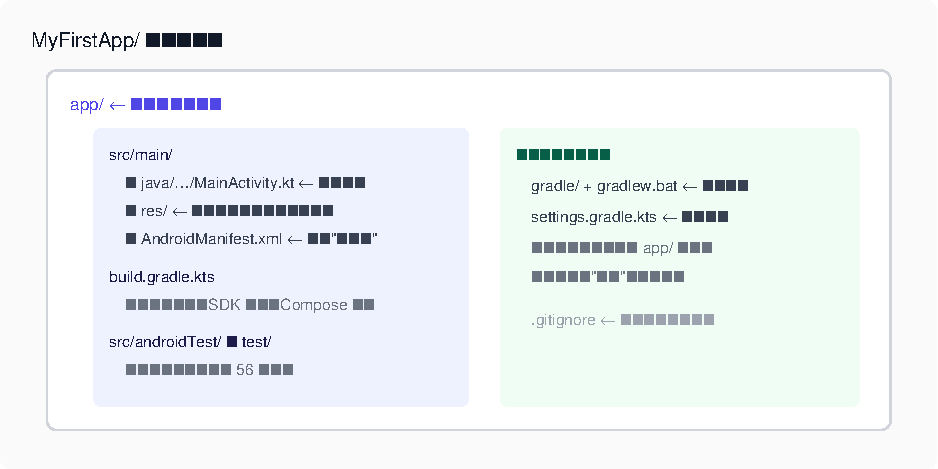
\includegraphics[width=0.92\linewidth]{figures/fig-di-si-shi-jiu-zhang-1}
\\[2pt]\small 图 2：新手必懂的工程结构（口诀：只碰 app/ 目录）
\end{center}

\begin{itemize}
  \item \textbf{MainActivity.kt}：App 的"大门"。用户点开图标，第一个被唤醒的就是它。现在的模板里它负责显示"Hello Android!"。
  \item \textbf{AndroidManifest.xml}：App 的"户口本"——声明这个 App 叫什么、图标是哪个、有哪些页面、要用哪些权限（相机、定位等）。
  \item \textbf{res/ 目录}：资源仓库，存图片、图标、字符串、颜色。把文字放资源文件而不是写死在代码里，是安卓开发的好习惯（换语言、换主题都方便）。
  \item \textbf{build.gradle.kts}：构建配方——声明最低支持版本、依赖哪些库（比如 Compose）。
\end{itemize}

\booksection{五、小试牛刀：把“Hello”换成你的名字}

打开 MainActivity.kt，你会看到 Compose 模板生成的代码。找到\texttt{Text(“Hello Android!”)}这一行，把引号里的字换成你的名字，比如\texttt{Text(“你好，张三！这是我的第一个App”)}，然后按Ctrl+R（Mac 是Cmd+R）重新运行。几秒后，模拟器上就显示了你的名字。

\begin{lstlisting}[language=Kotlin]
setContent {
    MyFirstAppTheme {
        Surface(modifier = Modifier.fillMaxSize()) {
            // v 把这里改成你自己的文字
            Text("你好，张三！这是我的第一个App")
        }
    }
}
\end{lstlisting}

恭喜，你已经完成了一次完整的“改代码 编译 安装 运行”循环。这个循环，就是未来每一天的开发日常。趁热打铁，试着再改点别的：把字号调大、换个颜色——下一章我们就会学到这些“魔法”是怎么来的。

\booksection{六、常见报错急救：新手前两周的“急诊室”}

环境搭建和首次构建阶段，你会大概率遇到下面三种报错。别慌，都有解药：

\begin{center}
\begin{tabularx}{\linewidth}{|X|X|X|}
\hline
\textbf{报错现象} & \textbf{常见原因} & \textbf{解药} \tabularnewline
\hline
Gradle sync failed / 依赖下载慢 & 网络访问仓库不畅 & 给 Gradle 配置国内镜像仓库（阿里云/腾讯云 maven 镜像），网上搜"gradle 国内镜像"照着改 \tabularnewline
SDK 组件缺失 & 安装时跳过了 SDK 下载 & Settings SDK Manager 补装缺失的平台与工具 \tabularnewline
模拟器启动失败 / 黑屏 & 虚拟化未开启、镜像损坏 & BIOS 开 VT-x/AMD-V；删掉模拟器重建；或直接用真机调试 \tabularnewline
\hline
\end{tabularx}
\end{center}

\begin{center}\small\color{gray}新手环境报错急救表\end{center}

\begin{tcbinfo}{小贴士：搜报错的方法论}
报错信息第一行是最有价值的——把它原样复制进搜索引擎，加“android studio”关键词。别搜“我装不上环境怎么办”这种笼统问题，搜“Gradle sync failed: Could not resolve com.android.tools.build”这种具体错误。精确的问题，才有精确的答案。

\end{tcbinfo}

\begin{tcbpractice}{来动手：完成你的"开发仪式感"清单}
(1) 装好 Android Studio 并跑通模拟器；(2) 用真机跑一次自己的 App 并截图留念；(3) 把 Hello 文字改成你的名字；(4) 把项目压缩存个档。做完这四步，你就可以在朋友圈宣布：我也是安卓开发者了（截图为证）。

\end{tcbpractice}

\begin{tcbsummary}{本章小结}
\begin{itemize}
  \item Android Studio = 官方免费 IDE；建议 16GB 内存 + 20GB 磁盘 + 开虚拟化
  \item 新建项目三要素：名字、包名（全球唯一，com.example 别上架）、最低 SDK（API 26 起）
  \item 两种运行方式：模拟器（电脑里虚拟手机）与真机（开 USB 调试，用完记得关）
  \item 工程口诀：只碰 app/ 目录——MainActivity.kt 是大门，Manifest 是户口本，res/ 是资源仓库
  \item 开发日常 = 改代码 Run 看效果，循环往复
\end{itemize}

\end{tcbsummary}

\bookchapter{第五十章：Kotlin 快速上手——安卓开发的第一语言}

\chapterintro{这一章咱们正式学语言。别紧张——Kotlin 是出了名的“对新手友好”，而且你不需要背语法书：先掌握 20\% 的语法，就能看懂和写出 80\% 的日常代码。剩下的边做项目边查。记住咱们的学习原则：\textbf{看懂 > 记住，会用 > 精通}。}

\booksection{一、变量与类型：给数据起名字}

程序就是“数据 + 逻辑”。变量，就是给数据起个名字存起来。Kotlin 有两种声明方式：

\begin{lstlisting}[language=Kotlin]
val name = "张三"        // val：只读变量（推荐默认用这个）
var age = 18             // var：可变变量（以后还能改）

age = 19                 // <i class="fas fa-check-circle mr-1"></i> var 可以改
// name = "李四"         // <i class="fas fa-times-circle mr-1"></i> val 不能改，编译会报错

val score: Int = 100     // 也可以显式写明类型
val pi = 3.14            // 不写也能自动推断
\end{lstlisting}

常用类型就几种，一张表记住：

\begin{center}
\begin{tabularx}{\linewidth}{|X|X|X|}
\hline
\textbf{类型} & \textbf{存什么} & \textbf{示例} \tabularnewline
\hline
Int & 整数 & 42 \tabularnewline
Double & 小数 & 3.14 \tabularnewline
String & 文字 & "你好" \tabularnewline
Boolean & 真/假 & true / false \tabularnewline
List< T> & 一组数据 & listOf(1, 2, 3) \tabularnewline
\hline
\end{tabularx}
\end{center}

\begin{center}\small\color{gray}Kotlin 常用基础类型\end{center}

\begin{tcbinfo}{小贴士：val 优先原则}
Kotlin 社区的铁律：\textbf{默认用 val，确有必要再用 var}。能用 val 的地方用 var，IDE 会黄字警告你。这个习惯能帮你少掉一大类“变量被意外修改”的 bug——代码越少变化，越容易推理。

\end{tcbinfo}

\booksection{二、函数：把逻辑打包成“按钮”}

函数是一段有名字的逻辑，像遥控器上的按钮——按一下（调用），就执行一串动作。Kotlin 里用\texttt{fun}声明：

\begin{lstlisting}[language=Kotlin]
fun greet(name: String): String {
    return "你好，$name！"     // $ 符号把变量插进字符串
}

println(greet("张三"))        // 输出：你好，张三！

// 单行函数可以简写成表达式
fun add(a: Int, b: Int) = a + b

println(add(3, 5))            // 输出：8
\end{lstlisting}

几个要点：参数写在括号里（名字在前、类型在后，用冒号隔开）；返回类型写在括号后；\textbf{字符串模板}\texttt{\$变量名}是 Kotlin 的招牌便利——不用再像 Java 那样“字符串 + 变量”地拼来拼去。

\booksection{三、条件与循环：让程序会“思考”}

程序的智能来自两件事：\textbf{会判断}（if/when）和\textbf{会重复}（for/while）。

\begin{lstlisting}[language=Kotlin]
// 判断：if / else
val age = 17
if (age >= 18) {
    println("成年人")
} else {
    println("未成年")
}

// 多分支：when（比 switch 好用一百倍）
val score = 85
val level = when {
    score >= 90 -> "优秀"
    score >= 60 -> "及格"
    else -> "再接再厉"
}

// 重复：for 循环
val fruits = listOf("苹果", "香蕉", "橙子")
for (fruit in fruits) {
    println("我爱吃$fruit")
}
\end{lstlisting}

\texttt{when}是 Kotlin 里最常用的多分支写法，安卓开发里你会天天用到它（比如根据状态显示不同界面）。

\booksection{四、空安全：Kotlin 的“保命符”}

Java 时代最著名的 bug 叫\textbf{NullPointerException（空指针异常）}——程序访问了一个“什么都没有”的东西，直接崩溃。据统计它是安卓崩溃排行榜的常年第一。Kotlin 从语言层面解决了它：\textbf{默认不允许空值}。

\begin{lstlisting}[language=Kotlin]
var name: String = "张三"   // 普通类型：绝不允许是 null
// name = null                // <i class="fas fa-times-circle mr-1"></i> 编译错误，直接把你拦住

var nickname: String? = null // 加个问号：允许为 null
nickname = "三儿"

// 使用可空类型时，必须安全地处理：
println(nickname?.length)    // 安全调用：null 就返回 null，不崩
val len = nickname?.length ?: 0   // Elvis 操作符：null 时给默认值
println(len)
\end{lstlisting}

\begin{tcbwarn}{注意：? 和 ?: 别搞混}
\texttt{String?}是“允许为空”，\texttt{a ?: b}是“a 为空时用 b”（长得像猫王发型，所以叫 Elvis 操作符）。刚开始写代码时，看到编译器报“null 相关错误”，八成是你忘了处理可空类型——这正是语言在保护你。

\end{tcbwarn}

\booksection{五、类与对象：造“零件”的模具}

类是对象的“模具”，对象是类的“成品”。安卓里的一切——页面、按钮、数据——都是对象。Kotlin 里有个神器叫\textbf{data class}（数据类），专门用来“装数据”，一行顶 Java 几十行：

\begin{lstlisting}[language=Kotlin]
// 普通类：模具
class Dog(val name: String) {
    fun bark() = println("$name 汪汪！")
}

val dog = Dog("旺财")      // 造对象
dog.bark()                 // 旺财 汪汪！

// data class：装数据的盒子（自动带 equals/copy 等）
data class User(val id: Int, val name: String, val email: String)

val me = User(1, "张三", "zhangsan@example.com")
val twin = me.copy(name = "张三丰")   // 复制并改一个字段
\end{lstlisting}

以后你做记账本，一笔账就是一个 data class：\texttt{data class Record(val amount: Double, val category: String, val date: String)}。看，你已经能写出真实项目的代码结构了。

\booksection{六、lambda 与高阶函数：Kotlin 的“语法糖”}

安卓代码里你会天天看到\texttt{\{ .\allowbreak .\allowbreak .\allowbreak  \}}这种“没名字的函数”，它叫\textbf{lambda（匿名函数）}。Button 的\texttt{onClick = \{ count++ \}}就是一个 lambda——把“点击后做什么”打包成一坨，递给按钮。

\begin{lstlisting}[language=Kotlin]
// 普通写法：定义一个有名函数再传入
fun double(x: Int) = x * 2
val result = listOf(1, 2, 3).map(::double)

// lambda 写法：就地定义，轻快直接
val result2 = listOf(1, 2, 3).map { it * 2 }   // it = 当前元素

// 筛选 + 变换连招（真实项目里极常见）
val bills = listOf(12.5, 88.0, 5.0, 200.0)
val bigBills = bills.filter { it > 50 }.sorted()
// [88.0, 200.0]——"超过 50 的账单，排好序"
\end{lstlisting}

几个高频“集合连招”记一下：\texttt{filter}（筛选）、\texttt{map}（变换）、\texttt{sorted}（排序）、\texttt{sum}（求和）。你未来 90\% 的列表处理，都是这四招的组合。Kotlin 的哲学就是：\textbf{能用一句话说清楚的逻辑，绝不写五句}。

\booksection{七、写给零基础的语法速查卡}

别试图一天背完所有语法。把这张卡存下来，写代码时对照着查，两周后自然就熟了：

\begin{center}
\begin{tabularx}{\linewidth}{|X|X|}
\hline
\textbf{要做什么} & \textbf{写法} \tabularnewline
\hline
定义只读变量 & \texttt{val x = 1} \tabularnewline
定义可变变量 & \texttt{var x = 1} \tabularnewline
定义函数 & \texttt{fun 名字(参数): 返回类型 \{ .\allowbreak .\allowbreak .\allowbreak  \}} \tabularnewline
判断 & \texttt{if (条件) \{.\allowbreak .\allowbreak .\allowbreak \} else \{.\allowbreak .\allowbreak .\allowbreak \}} \tabularnewline
多分支 & \texttt{when \{ 条件 -\allowbreak > 结果 \}} \tabularnewline
遍历 & \texttt{for (x in 列表) \{ .\allowbreak .\allowbreak .\allowbreak  \}} \tabularnewline
字符串拼接 & \texttt{"你好，\$name"} \tabularnewline
处理可空 & \texttt{x?.\allowbreak length ?: 0} \tabularnewline
定义数据类 & \texttt{data class X(val a: Int, val b: String)} \tabularnewline
\hline
\end{tabularx}
\end{center}

\begin{center}\small\color{gray}Kotlin 语法速查卡（新手版）\end{center}

\begin{tcbpractice}{来动手：不装任何软件，先玩 10 分钟 Kotlin}
浏览器打开 play.kotlinlang.org（Kotlin 官方在线演练场），把本章的每一段代码都粘进去跑一遍，改改数字和文字，看看输出怎么变。这个“先玩后学”的 10 分钟，会让你第 51 章上手时轻松一倍。

\end{tcbpractice}

\begin{tcbsummary}{本章小结}
\begin{itemize}
  \item val 优先，var 慎用；类型可自动推断，冒号后显式声明也行
  \item 函数 = 打包的逻辑；字符串模板 \$ 是招牌便利
  \item if/when 判断，for 循环；when 是安卓开发里的"多面手"
  \item 空安全是 Kotlin 的保命符：普通类型拒绝 null，可空类型必须 ? / ?: 处理
  \item data class 是装数据的盒子，一个字段一行，真实项目天天用
  \item 20\% 语法干 80\% 的活：先会用，再精通
\end{itemize}

\end{tcbsummary}

\bookchapter{第五十一章：界面开发——Jetpack Compose 入门}

\chapterintro{界面是用户看到的一切。在 Compose 出现之前，安卓界面用 XML 写——像填空题一样繁琐；2021 年谷歌推出了\textbf{Jetpack Compose}：直接用 Kotlin 代码“画”界面，所见即所得，改一行代码预览立刻刷新。到 2026 年，Compose 已是新项目的绝对主流。这一章，咱们学会“画画”。}

\booksection{一、Compose 的思想：界面就是函数}

Compose 的核心思想一句话：\textbf{界面 = 函数}。每个能显示在屏幕上的东西（文字、按钮、图片）都是一个“可组合函数”（Composable），用\texttt{@Composable}标记。把它们像积木一样嵌套起来，就是界面。

\begin{lstlisting}[language=Kotlin]
@Composable
fun Greeting(name: String) {
    Text(text = "你好，$name！")     // 一个"文字积木"
}

// 嵌套组合：大积木套小积木
@Composable
fun HomeScreen() {
    Column {                          // 竖着排列
        Greeting(name = "张三")
        Greeting(name = "李四")
        Button(onClick = { /* 点击做什么 */ }) {
            Text("点我")
        }
    }
}
\end{lstlisting}

注意\texttt{@Composable}这个“帽子”——它告诉编译器“这是一个界面积木”。积木可以无限嵌套，这就是 Compose 的全部秘密。

\booksection{二、基础组件：文字、按钮、输入框、图片}

Compose 的组件就是“积木块”，最常见的四种：

\begin{center}
\begin{tabularx}{\linewidth}{|X|X|X|}
\hline
\textbf{组件} & \textbf{干什么} & \textbf{必备参数} \tabularnewline
\hline
Text & 显示文字 & text（要显示的字） \tabularnewline
Button & 按钮 & onClick（点击回调） \tabularnewline
TextField & 输入框 & value、onValueChange（输入变化回调） \tabularnewline
Image & 显示图片 & painter（图片资源） \tabularnewline
\hline
\end{tabularx}
\end{center}

\begin{center}\small\color{gray}Compose 四大基础组件\end{center}

\begin{lstlisting}[language=Kotlin]
@Composable
fun BasicWidgets() {
    Column {
        Text(text = "这是一段文字")
        Button(onClick = { println("被点击了") }) {
            Text("按钮")
        }
        var input by remember { mutableStateOf("") }
        TextField(
            value = input,
            onValueChange = { input = it },
            label = { Text("输入点什么") }
        )
    }
}
\end{lstlisting}

输入框那两行里出现了\texttt{remember \{ mutableStateOf(“”) \}}——这就是 Compose 的“状态”魔法，本章第五节细讲。现在先混个脸熟。

\booksection{三、布局三件套：Column、Row、Box}

组件有了，怎么摆放？记住三个“盒子”：

\begin{itemize}
  \item \textbf{Column}：竖着排（像排队打饭）；
  \item \textbf{Row}：横着排（像并排坐）；
  \item \textbf{Box}：叠着放（像扑克牌摞一起，适合做角标、遮罩）。
\end{itemize}

\begin{lstlisting}[language=Kotlin]
Column {
    Text("第一行")
    Row {
        Text("左边")
        Text("右边")
    }
    Box {
        Text("底层")
        Text("叠在上面的角标")
    }
}
\end{lstlisting}

想让布局更好看？给组件加\textbf{Modifier}（修饰符）——它就像给积木“上妆”：

\begin{lstlisting}[language=Kotlin]
Text(
    text = "好看的文字",
    modifier = Modifier
        .padding(16.dp)          // 四周留白
        .fillMaxWidth()          // 撑满宽度
        .background(Color.Blue)  // 背景色
        .clickable { /* 点击 */ }// 可点击
)
// 链式调用：一个接一个，顺序有意义（先 padding 再背景，背景不含边距）
\end{lstlisting}

\begin{tcbwarn}{注意：Modifier 的顺序有讲究}
\texttt{padding(16.\allowbreak dp).\allowbreak background(Blue)}和\texttt{background(Blue).\allowbreak padding(16.\allowbreak dp)}效果不同——前者是“先留白再涂色”（背景不含边距），后者是“先涂色再留白”（背景包含边距）。新手最容易在这上面画错“奇怪的白边”。不确定时，调换顺序试试，预览立刻告诉你答案。

\end{tcbwarn}

\booksection{四、状态：让界面“活”起来}

静态界面没意思。想让按钮点击后数字 +1、输入框能打字，就需要\textbf{状态（State）}。Compose 的规则：\textbf{界面永远忠实反映状态，状态变了，界面自动重画}。

\begin{lstlisting}[language=Kotlin]
@Composable
fun Counter() {
    // remember + mutableStateOf：记住这个会变化的值
    var count by remember { mutableStateOf(0) }

    Column {
        Text(text = "你点了 $count 次")
        Button(onClick = { count++ }) {   // 改状态
            Text("点我 +1")                // 界面自动刷新
        }
    }
}
\end{lstlisting}

三行代码，一个活的计数器。这就是 Compose 比老式写法爽的地方：\textbf{不用手动“刷新界面”，改数据就行}。记住两个关键函数：\texttt{remember}（让值在界面重组时不被清空）和\texttt{mutableStateOf}（告诉 Compose“这个值变了要重画”）。

用户点击

状态改变（count++）

Compose 感知到变化

自动重画界面（重组）

\begin{center}\small\color{gray}图 3：Compose 的“状态 界面”单向数据流\end{center}

\booksection{五、主题与深色模式：一次配置，全局生效}

模板项目里的\texttt{MyFirstAppTheme \{ .\allowbreak .\allowbreak .\allowbreak  \}}就是主题。它基于\textbf{Material 3}设计规范，帮你把颜色、字体、形状统一管理。支持深色模式只需三步：

\begin{enumerate}
  \item 在主题里定义好浅色/深色两套配色（模板已自动生成\texttt{ColorScheme}）；
  \item 系统切到深色模式时，\texttt{isSystemInDarkTheme()}自动判断；
  \item 用主题提供的颜色（如\texttt{MaterialTheme.\allowbreak colorScheme.\allowbreak primary}）而不是写死颜色值。
\end{enumerate}

\begin{tcbinfo}{小贴士：Material 3 动态取色}
Android 12 起的“Material You”能让 App 从你的壁纸里提取颜色。Compose 模板默认支持（\texttt{dynamicColor}）。你的 App 在不同用户手机上会“自动换装”，这就是现代安卓的浪漫。

\end{tcbinfo}

\booksection{六、预览、动画与实时编辑：Compose 的“外挂”}

Compose 三个开发体验上的“外挂”，用上就回不去：

\begin{itemize}
  \item \textbf{@Preview 预览}：给 Composable 加\texttt{@Preview}注解，Android Studio 右侧立刻渲染出界面——改代码所见即所得，不用每次装到手机上；
  \item \textbf{实时编辑（Live Edit）}：2026 年的 Android Studio 支持在模拟器/真机上"热更新"部分改动，改文字颜色之类的小调整，设备上秒变；
  \item \textbf{动画 API}：\texttt{animateFloatAsState}、\texttt{AnimatedVisibility}几行代码就能让元素平滑过渡——"高级感"往往就差这几十行。
\end{itemize}

\begin{lstlisting}[language=Kotlin]
@Composable
fun AnimatedBox() {
    var big by remember { mutableStateOf(false) }
    // 值变化时自动平滑过渡到目标值
    val size by animateDpAsState(if (big) 120.dp else 60.dp)

    Box(Modifier
        .size(size)
        .background(MaterialTheme.colorScheme.primary)
        .clickable { big = !big }
    )
}
\end{lstlisting}

\begin{tcbinfo}{小贴士：先功能后动画}
新手常犯的毛病是“界面还没做对，就开始纠结动画”。先让功能跑通，最后再统一加动效——这也是“简单至上”原则：\textbf{动画是锦上添花，功能是雪中送炭}。

\end{tcbinfo}

\begin{tcbpractice}{来动手：做一个"心情按钮"}
把模板项目改成一个心情切换器：一个按钮，点击后在 开心 难过 生气 之间循环切换，文字和背景色跟着变。提示：用\texttt{when}根据状态选文案和颜色。做完发给朋友玩，收获第一波“哇你会做 App 了”。

\end{tcbpractice}

\begin{tcbsummary}{本章小结}
\begin{itemize}
  \item Compose 思想：界面 = @Composable 函数，积木式嵌套
  \item 四大组件：Text / Button / TextField / Image
  \item 布局三件套：Column 竖排、Row 横排、Box 叠放
  \item Modifier 链式"上妆"：padding、fillMaxWidth、background、clickable——顺序有意义
  \item 状态是灵魂：remember + mutableStateOf，改数据界面自动重画
  \item 主题用 Material 3 + 动态取色，深色模式一次配置全局生效
\end{itemize}

\end{tcbsummary}

\bookchapter{第五十二章：四大组件与 Activity 生命周期}

\chapterintro{如果说 Compose 是 App 的“脸”，那这一章讲的就是 App 的“骨架”。安卓系统有四大基本组件，所有 App 都是由它们拼成的；而其中最重要的 Activity，有一张每个安卓开发者都必须刻在脑子里的“生命周期图”。本章学完，你就能理解“为什么切个后台回来，我的 App 状态就没了”这类千古之谜。}

\booksection{一、四大组件：安卓的“四梁八柱”}

安卓官方定义了四种基本组件，分别负责一类工作：

\begin{center}
\begin{tabularx}{\linewidth}{|X|X|X|}
\hline
\textbf{组件} & \textbf{职责} & \textbf{打个比方} \tabularnewline
\hline
Activity & 一个可见的界面 & 店铺的门面——用户能看见、能交互 \tabularnewline
Service & 后台干活的"隐形人" & 仓库工人——放音乐、下载文件，不需要界面 \tabularnewline
BroadcastReceiver & 接收系统广播 & 传达室——"电池没电了""网络断了"的喇叭 \tabularnewline
ContentProvider & 跨 App 共享数据 & 公共资料柜——比如把联系人共享给别的 App \tabularnewline
\hline
\end{tabularx}
\end{center}

\begin{center}\small\color{gray}安卓四大组件速览\end{center}

新手阶段你 95\% 的时间都在跟\textbf{Activity}打交道；Service 和 BroadcastReceiver 做音乐播放、消息推送时会用到；ContentProvider 用得最少（系统已把常用数据封好了）。另外注意：四大组件都要在\textbf{AndroidManifest.xml}里“登记户口”，不登记系统就找不到它们。

\booksection{二、Activity 生命周期：安卓开发的第一张“藏宝图”}

手机上的 App 随时可能被打断：来电话了、用户切去回微信、系统内存不够把你杀了……Activity 的一生，就是在这张图上循环旅行：

onCreate（出生：初始化）

onStart（可见了）

onResume（前台交互中）

onPause（部分被遮住）

onStop（完全看不见）

onDestroy（销毁）

onRestart / onStart / onResume：回到前台时原路返回

\begin{center}\small\color{gray}图 4：Activity 生命周期（前进方向：上排出生 下排离场，回来时原路折返）\end{center}

\begin{center}
\begin{tabularx}{\linewidth}{|X|X|X|}
\hline
\textbf{回调} & \textbf{什么时候触发} & \textbf{典型用途} \tabularnewline
\hline
onCreate & Activity 创建时（一次） & 加载界面、初始化数据 \tabularnewline
onStart & 界面变为可见 & 开始一些轻量逻辑 \tabularnewline
onResume & 拿到焦点、可交互 & 开始动画、恢复播放 \tabularnewline
onPause & 被部分遮挡/切走瞬间 & 暂停动画、保存草稿 \tabularnewline
onStop & 完全不可见 & 释放重资源、暂停下载 \tabularnewline
onDestroy & 被销毁前 & 最后的清理 \tabularnewline
\hline
\end{tabularx}
\end{center}

\begin{center}\small\color{gray}六个生命周期回调的典型用途\end{center}

\textbf{避坑提醒：屏幕旋转会“杀死”Activity}\par

新手最经典的翻车现场：App 转一下屏幕，输入框里的字全没了。原因：旋转屏幕默认会销毁并重建 Activity（走一遍 onDestroy onCreate）。解法：用\texttt{rememberSaveable}保存状态（Compose 里替代 remember），它会在重建时自动把值找回来。第 6、7 章会反复用到。

\booksection{三、Intent：App 里外通行的“车票”}

Intent（意图）是组件之间通信的“车票”。你想从一个页面跳到另一个页面，或者打开浏览器、调起相机，都要“买票上车”：

\begin{lstlisting}[language=Kotlin]
// 方式一：显式 Intent——明确指定去哪个页面
val intent = Intent(this, DetailActivity::class.java)
intent.putExtra("name", "张三")     // 车上捎带"行李"（数据）
startActivity(intent)

// 方式二：隐式 Intent——只说要干什么，系统找谁干
val web = Intent(Intent.ACTION_VIEW, Uri.parse("https://developer.android.com"))
startActivity(web)   // 系统会打开浏览器/或让你选
\end{lstlisting}

两种方式各有用途：\textbf{显式}用于自己 App 内部的页面跳转；\textbf{隐式}用于调用系统或其他 App 的能力（开网页、打电话、分享）。Compose 项目里，在 Composable 中用\texttt{LocalContext.current}拿到 Context 就能\texttt{startActivity}。

\booksection{四、多页面与导航}

真实 App 都有多个页面。Compose 官方推荐的导航方案是\textbf{Navigation Compose}（依赖库 androidx.navigation）：

\begin{lstlisting}[language=Kotlin]
val navController = rememberNavController()

NavHost(navController, startDestination = "home") {
    composable("home") { HomeScreen(navController) }
    composable("detail/{name}") { entry ->
        val name = entry.arguments?.getString("name")
        DetailScreen(name ?: "未知")
    }
}

// 在页面里跳转：
navController.navigate("detail/张三")     // 带参数
navController.popBackStack()              // 返回上一页
\end{lstlisting}

\begin{tcbinfo}{小贴士：页面多了怎么办？}
项目长大后，把所有页面路由集中写在一个文件里（比如\texttt{AppNavGraph.kt}），统一管理，别让“跳转到哪”的逻辑散落在各个页面。这是从“能跑”走向“可维护”的第一步。

\end{tcbinfo}

\booksection{五、顺带认识：Fragment 是什么（以及为什么本书没教）}

查老教程时你一定会撞见\textbf{Fragment}——它是 Activity 里的“可复用界面片段”，在老式多页面架构里是绝对主角。但 Compose 时代，页面直接用 Composable 函数 + Navigation 路由就够了，官方也已弱化 Fragment 的地位。本书因此没把它放进主线。

给你的建议：\textbf{新项目不主动用 Fragment}；但读老代码、面试被问到时，知道它是“Activity 里嵌的界面片段”即可。学习资源永远优先选 2023 年以后的——安卓技术栈的“老黄历”更新得比想象中快。

\begin{tcbpractice}{来动手：给计数器装上"记忆"}
把第 51 章的计数器改造一下：(1) 把 remember 换成 rememberSaveable，旋转屏幕验证数字还在；(2) 加一个“关于”按钮，用 Navigation 跳到第二个页面显示版本号；(3) 在两个页面的 onCreate/onPause 里打印日志（Log.d），用 Logcat 观察生命周期调用顺序。做完这三步，生命周期就不再是纸上谈兵。

\end{tcbpractice}

\begin{tcbsummary}{本章小结}
\begin{itemize}
  \item 四大组件：Activity（门面）、Service（后台）、BroadcastReceiver（喇叭）、ContentProvider（资料柜）
  \item 生命周期六回调：onCreate onStart onResume onPause onStop onDestroy
  \item 旋转屏幕会销毁重建 Activity：用 rememberSaveable 保住状态
  \item Intent 是"车票"：显式跳自家页面，隐式调系统能力
  \item 多页面用 Navigation Compose：NavHost + composable 路由
\end{itemize}

\end{tcbsummary}

\bookchapter{第五十三章：数据存储与网络请求}

\chapterintro{一个只能“看”的 App 是死的；能存数据、能连网络的 App 才是活的。这一章认识安卓数据层的“三件套”：DataStore（存小配置）、Room（存结构化数据）、Retrofit（和服务器对话），外加它们的“总调度”——协程。学完这章，你就能写会记住用户习惯、会实时更新内容的真 App 了。}

\booksection{一、存储方案怎么选：先看这张表}

\begin{center}
\begin{tabularx}{\linewidth}{|X|X|X|X|}
\hline
\textbf{方案} & \textbf{适合存什么} & \textbf{特点} & \textbf{本书哪里用} \tabularnewline
\hline
DataStore & 零散配置（主题、开关） & 键值对，简单安全 & 第 54 章记账本设置 \tabularnewline
Room & 结构化数据（账目、用户） & 真正的 SQLite 数据库封装，可查询 & 第 54 章账目记录 \tabularnewline
Retrofit & （不存，联网取）服务器数据 & HTTP 请求库的事实标准 & 第 55 章天气数据 \tabularnewline
\hline
\end{tabularx}
\end{center}

\begin{center}\small\color{gray}数据三件套的分工\end{center}

记一个口诀：\textbf{“小配置进 DataStore，成批数据进 Room，外面的数据走 Retrofit”}。旧教程里常见的 SharedPreferences 已被 DataStore 取代，SQLite 手写 SQL 也已被 Room 取代——直接学新的，别走老路。

\booksection{二、DataStore：存点小配置}

想记住“用户上次选的币种”“是否开启深色模式”这类零散值，用 DataStore（Preferences 版）：

\begin{lstlisting}[language=Kotlin]
val Context.dataStore by preferencesDataStore(name = "settings")

// 写：存一个值
suspend fun saveTheme(isDark: Boolean) {
    context.dataStore.edit { prefs ->
        prefs[THEME_KEY] = isDark
    }
}

// 读：取出来（Flow 会自动通知变化）
val themeFlow: Flow<Boolean> = context.dataStore.data
    .map { it[THEME_KEY] ?: false }
\end{lstlisting}

注意返回的是\textbf{Flow}——一个会“流动”的数据流。值一旦改变，所有观察它的地方自动收到新值。这个概念（响应式）是安卓现代的基石，第 54 章会实战。

\booksection{三、Room：给数据安个“真正的家”}

记账本有成百上千笔账，还要按分类、按月份查询统计——这需要数据库。Room 是 SQLite 的官方封装，把“建表、查数据”变得像写 Kotlin 一样自然。三样东西：

\begin{lstlisting}[language=Kotlin]
// 1. Entity：表结构（一张表 = 一个 data class）
@Entity(tableName = "records")
data class Record(
    @PrimaryKey(autoGenerate = true) val id: Long = 0,
    val amount: Double,
    val category: String,
    val note: String,
    val date: String
)

// 2. Dao：操作接口（增删改查）
@Dao
interface RecordDao {
    @Query("SELECT * FROM records ORDER BY date DESC")
    fun getAll(): Flow<List<Record>>

    @Insert
    suspend fun insert(record: Record)

    @Delete
    suspend fun delete(record: Record)

    @Query("SELECT SUM(amount) FROM records WHERE category = :c")
    suspend fun sumByCategory(c: String): Double
}

// 3. Database：总装
@Database(entities = [Record::class], version = 1)
abstract class AppDatabase : RoomDatabase() {
    abstract fun recordDao(): RecordDao
}
\end{lstlisting}

这套“三件套”模板可以原样搬进你的任何项目——换换字段名就行。查询返回 Flow，界面跟着数据自动刷新，妙不可言。

\booksection{四、Retrofit：和服务器说话}

天气、新闻、汇率……这些数据不在手机里，在别人的服务器上。Retrofit 让“向服务器要数据”变得像调函数一样简单。三步走：

\begin{lstlisting}[language=Kotlin]
// 1. 定义接口：把 HTTP 请求描述成函数
interface WeatherApi {
    @GET("v1/weather")
    suspend fun getWeather(@Query("city") city: String): WeatherResponse
}

// 2. 创建实例
val api = Retrofit.Builder()
    .baseUrl("https://api.example.com/")
    .addConverterFactory(GsonConverterFactory.create())
    .build()
    .create(WeatherApi::class.java)

// 3. 像调函数一样调用（在协程里）
val result = api.getWeather("北京")
\end{lstlisting}

\textbf{避坑提醒：两条网络铁律}\par

(1)\textbf{网络请求绝不能在主线程做}——会卡死界面甚至崩溃（NetworkOnMainThreadException）。所有网络调用必须放在协程（viewModelScope.launch）里。(2) 明文 HTTP 默认被禁止：安卓 9 起要求 HTTPS。测试时若要用 http:// 的本地地址，需要在 Manifest 里显式声明\texttt{usesCleartextTraffic}——但正式产品必须全走 HTTPS。

\booksection{五、JSON 解析：给网络数据“翻译”}

服务器返回的数据大多是 JSON——一串像“嵌套字典”的文本。Retrofit 需要一个“翻译官”把它变成 Kotlin 对象。2026 年的两大主流方案：

\begin{center}
\begin{tabularx}{\linewidth}{|X|X|X|}
\hline
\textbf{方案} & \textbf{特点} & \textbf{推荐场景} \tabularnewline
\hline
Gson / Moshi & 老牌反射方案，配置零成本 & 快速起步、字段不多的小项目 \tabularnewline
kotlinx.serialization & 官方编译期方案，更快更安全 & 新项目首选（2026 年主流） \tabularnewline
\hline
\end{tabularx}
\end{center}

\begin{center}\small\color{gray}JSON 解析两大方案\end{center}

\begin{lstlisting}[language=Kotlin]
// 给数据类加 @Serializable 注解
@Serializable
data class WeatherResponse(
    val weather: List<Weather>,
    val main: Main,
    val name: String
)

// Retrofit 挂上对应 Converter（以 Retrofit 2.11+ 官方支持为例）：
// .addConverterFactory(json.asConverterFactory("application/json".toMediaType()))
\end{lstlisting}

无论哪种方案，铁律都是：\textbf{先看真实返回的 JSON，再定义字段}。很多“解析失败”的 bug，都是因为字段名写错、嵌套层级猜错——把原始 JSON 打印出来对照，十秒定位。

\booksection{六、协程：安卓并发的“普通话”}

\booksection{五、协程：安卓并发的“普通话”}

上面反复出现的\texttt{suspend}和\texttt{launch}来自 Kotlin 协程（Coroutine）——安卓官方的并发方案。你可以粗暴地理解为：\textbf{让“要等一会儿”的操作（网络、数据库）不阻塞界面}。

\begin{lstlisting}[language=Kotlin]
// 在 ViewModel 里启动协程
viewModelScope.launch {
    val records = dao.getAll().first()  // suspend：会自动挂起等待
    // 更新界面状态……
}

// 关键词速记：
// suspend   —— "我要等待，别拦着别人"
// launch    —— "开工！"
// viewModelScope —— 跟着页面走的"工作间"，页面销毁自动收工
\end{lstlisting}

零基础先记住用法就好，背后的“挂起与恢复”原理可以以后再深究。日常开发你写的 90\% 都是这个模板。

\begin{tcbpractice}{来动手：做一个"每日一句"小应用}
找一个免费的名言 API（比如 hitokoto 之类），用 Retrofit 拉取“每日一句”，显示在屏幕中央，加个“换一句”按钮（协程里重新请求）。再把喜欢的句子用 Room 存进“收藏夹”。这个练习把 DataStore/Room/Retrofit/协程全用了一遍——做完它，第 7、8 章就是小菜一碟。

\end{tcbpractice}

\begin{tcbsummary}{本章小结}
\begin{itemize}
  \item 口诀：小配置进 DataStore，成批数据进 Room，外面的数据走 Retrofit
  \item DataStore 返回 Flow：值变了，观察者自动收到
  \item Room 三件套：@Entity（表）+ @Dao（操作）+ @Database（总装），模板可直接复用
  \item Retrofit 三步：定义接口 创建实例 协程里调用
  \item 两条铁律：网络不进主线程；正式产品必须 HTTPS
  \item 协程 = 不阻塞界面的等待；viewModelScope 是页面专属工作间
\end{itemize}

\end{tcbsummary}

\bookchapter{第五十四章：项目一——我的记账本（本地版）}

\chapterintro{欢迎来到你的第一个“正经项目”。这个记账本虽然不联网，但五脏俱全：能记一笔账、能看流水、能按月统计、能删改。做完它，你就完整走了一遍“数据 逻辑 界面”的全流程。别急着抄代码——\textbf{先想清楚再动手}，这是咱们一贯的原则。}

\booksection{一、需求思考：先问五个问题}

动手之前，用“需求五要素”把想法捋清楚：

\begin{center}
\begin{tabularx}{\linewidth}{|X|X|}
\hline
\textbf{要素} & \textbf{答案} \tabularnewline
\hline
Who（给谁用） & 自己用，家人朋友也行 \tabularnewline
What（做什么） & 记收支、看流水、按月汇总、按分类统计 \tabularnewline
Why（为什么） & 练手 + 搞清楚钱花哪儿了 \tabularnewline
How（怎么做） & Kotlin + Compose + Room + MVVM，纯本地无后端 \tabularnewline
Constraint（约束） & 一周内完成；最低支持 Android 8；不上架也先按上架标准写 \tabularnewline
\hline
\end{tabularx}
\end{center}

\begin{center}\small\color{gray}记账本需求五要素\end{center}

然后拆解成“每一步都能用”的小步骤：(1) 建 Room 数据层（能存一笔账）；(2) 列表页（能看流水）；(3) 录入页（能加账）；(4) 删除与编辑；(5) 月度汇总卡片。每完成一步，App 都是一个“能用的东西”。

\booksection{二、数据层：让“账”有个家}

先定义一笔账长什么样——字段要够用但别贪多：

\begin{lstlisting}[language=Kotlin]
@Entity(tableName = "records")
data class Record(
    @PrimaryKey(autoGenerate = true) val id: Long = 0,
    val type: String,        // "income" 收入 | "expense" 支出
    val amount: Double,      // 金额（元）
    val category: String,    // 分类：餐饮、交通、工资……
    val note: String = "",   // 备注（可选）
    val date: String         // "2026-08-15"
)
\end{lstlisting}

Dao 里加两条“统计用”的查询——这是记账本的灵魂：

\begin{lstlisting}[language=Kotlin]
@Dao
interface RecordDao {
    @Query("SELECT * FROM records ORDER BY date DESC, id DESC")
    fun getAll(): Flow<List<Record>>

    @Insert
    suspend fun insert(record: Record)

    @Delete
    suspend fun delete(record: Record)

    @Query("SELECT COALESCE(SUM(amount),0) FROM records WHERE type='income' AND date LIKE :month || '%'")
    suspend fun monthIncome(month: String): Double   // month 形如 "2026-08"

    @Query("SELECT COALESCE(SUM(amount),0) FROM records WHERE type='expense' AND date LIKE :month || '%'")
    suspend fun monthExpense(month: String): Double
}
\end{lstlisting}

\begin{tcbinfo}{小贴士：金额为什么用 Double？}
严谨的金融 App 会用 BigDecimal 或“以分为单位的 Int”来避免浮点误差（0.1+0.2$\neq$0.3 的老问题）。练手项目用 Double 足够；如果哪天做真金融产品，记得换成“分”为单位——这是无数前辈踩出来的坑。

\end{tcbinfo}

\booksection{三、MVVM：界面与逻辑“分家”}

直接让界面操作数据库？能跑，但界面代码会又臭又长。MVVM 架构让各司其职：\textbf{View（界面）只管画，ViewModel（逻辑中枢）管数据，Model（Room）管存储}。

View（Compose 界面）

ViewModel（状态与逻辑）

Model（Room 数据层）

\begin{center}\small\color{gray}图 5：MVVM 三层结构——数据单向流动，各层互不越界\end{center}

\begin{lstlisting}[language=Kotlin]
class RecordViewModel(private val dao: RecordDao) : ViewModel() {

    // 把 Flow 转成界面能观察的状态
    val records = dao.getAll()
        .stateIn(viewModelScope, SharingStarted.WhileSubscribed(), emptyList())

    // 用户操作：调用 suspend 函数
    fun addRecord(type: String, amount: Double, category: String, note: String, date: String) {
        viewModelScope.launch {
            dao.insert(Record(type = type, amount = amount,
                category = category, note = note, date = date))
        }
    }

    fun deleteRecord(record: Record) {
        viewModelScope.launch { dao.delete(record) }
    }
}
\end{lstlisting}

界面（Compose）里这样用：\texttt{val vm: RecordViewModel = viewModel()}，然后\texttt{val list by vm.records.collectAsState()}——数据一变，列表自动刷新，你什么都不用做。这就是 MVVM + Flow + Compose 三剑合璧的威力。

\booksection{四、界面：列表页 + 录入页}

列表页用\textbf{LazyColumn}（懒加载列表）——数据再多也不卡：

\begin{lstlisting}[language=Kotlin]
@Composable
fun RecordListScreen(vm: RecordViewModel) {
    val records by vm.records.collectAsState()

    Column {
        // 顶部汇总卡片（收入-支出=结余）
        SummaryCard(records)

        // 流水列表
        LazyColumn {
            items(records, key = { it.id }) { record ->
                RecordRow(record) { vm.deleteRecord(record) }
            }
        }

        // 悬浮"记一笔"按钮  弹录入对话框
        FloatingActionButton(onClick = { showAddDialog = true }) {
            Text("+")
        }
    }
}

@Composable
fun RecordRow(record: Record, onDelete: () -> Unit) {
    Row(Modifier.fillMaxWidth().padding(12.dp)) {
        Text(record.category, fontWeight = FontWeight.Bold)
        Spacer(Modifier.weight(1f))
        Text(if (record.type == "income") "+${record.amount}" else "-${record.amount}",
             color = if (record.type == "income") Color(0xFF27AE60) else Color(0xFFC0392B))
    }
}
\end{lstlisting}

录入用\textbf{AlertDialog}（对话框）最省事：几个输入框 + 收入/支出切换 + 分类下拉，点确定就调\texttt{vm.addRecord(...)}。

\begin{tcbwarn}{注意：输入校验别偷懒}
金额输入框一定要校验：空值、负数、“abc”这类非法输入都要拦住（用\texttt{toDoubleOrNull()}判断）。App 崩掉最常见的原因之一就是“把用户的输入当成了乖孩子”。记住：\textbf{用户输入的一切，都要当敌人审查}。

\end{tcbwarn}

\booksection{五、编辑与删除：让数据“能进能出”}

只会加不会删的记账本，用三天就废了。补两个操作：

\begin{lstlisting}[language=Kotlin]
// Dao 里补两条：
@Query("UPDATE records SET amount=:amount, category=:category, note=:note WHERE id=:id")
suspend fun update(id: Long, amount: Double, category: String, note: String)

@Query("DELETE FROM records WHERE id=:id")
suspend fun deleteById(id: Long)

// 界面上：长按列表项弹"编辑/删除"菜单（Compose 用 DropdownMenu 或 AlertDialog）
// 删除前最好弹确认框——"误删"是记账类 App 用户最痛恨的事
\end{lstlisting}

交互细节两条经验：\textbf{删除必须二次确认}（防止手滑），编辑尽量\textbf{预填原值}（改一个字比重新输入省事）。别小看这两个细节——产品感就是这些细节堆出来的。

\booksection{六、验收：三层检查 + 两个进阶挑战}

项目做完，按“功能 边界 架构”三层验收：能不能记、能不能删、重开 App 数据还在不在（功能）；金额输 0 或负数会不会崩、转屏会不会丢数据（边界）；界面和数据有没有混在一起、字段有没有硬编码（架构）。

基础版验收通过后，给自己加两道“进阶菜”：

\begin{enumerate}
  \item \textbf{月度筛选}：顶部加月份切换（比如 2026-08 v），列表只显示当月流水；
  \item \textbf{分类饼图}：用 Compose 的 Canvas 或引入轻量图表库，把"钱花哪儿了"画成饼图——做完这个，记账本就有点"产品样"了。
\end{enumerate}

\begin{tcbpractice}{来动手：本周完成它}
按“数据层 ViewModel 列表页 录入页 汇总卡片”的顺序动手，每天一步。卡住了就把报错原样丢给搜索引擎或 AI（还记得第七篇《AI编程实战篇》吗？描述问题时说清“期望行为、实际行为、复现步骤”）。完成后用它记一周账——自己做的 App 用起来，成就感会推着你继续往前走。

\end{tcbpractice}

\begin{tcbsummary}{本章小结}
\begin{itemize}
  \item 需求五要素 拆成"每步能用"的小步骤，再动手
  \item 数据层：Record 实体 + Dao（含月份统计 SQL）+ Database
  \item MVVM 分工：View 只管画，ViewModel 管逻辑，Model 管存储
  \item Flow + stateIn + collectAsState：数据一变界面自动刷新
  \item LazyColumn 懒加载列表；AlertDialog 做录入
  \item 三层验收（功能/边界/架构）+ 进阶挑战（月度筛选、分类饼图）
\end{itemize}

\end{tcbsummary}

\bookchapter{第五十五章：项目二——天气查询 App（网络版）}

\chapterintro{记账本是“练内功”，天气 App 是“见世面”——它要和互联网打交道。这个项目你会学到：申请免费 API、解析 JSON、处理“加载中/成功/失败”三种界面状态，以及怎么把 API 密钥藏好。做完它，你就具备了做任何“联网 App”的能力——新闻、汇率、翻译，套路一模一样。}

\booksection{一、申请免费天气 API}

个人练手，推荐\textbf{OpenWeatherMap}或国内的\textbf{和风天气（QWeather）}——都有免费额度，注册即用。以 OpenWeatherMap 为例：

\begin{enumerate}
  \item 注册账号 在 API keys 页面生成一个 Key（\texttt{apikey}）；
  \item 免费版可调用 Current Weather（当前天气）接口：\texttt{api.openweathermap.org/data/2.5/weather?q=beijing\&appid=你的Key\&units=metric}；
  \item 浏览器里先试一次，看看返回的 JSON 长什么样——这是接任何 API 前必做的"预习"。
\end{enumerate}

\textbf{避坑提醒：密钥绝不能写死在代码里}\par

API Key 相当于你的“钱包密码”，写进代码一提交到 GitHub，几小时内就会被爬虫扫走盗刷。正确做法：放进\texttt{local.properties}（这个文件已被 gitignore 忽略），再通过 Gradle 的 buildConfig 读进代码。搜索“Android 隐藏 API Key 的最佳实践”照着改即可。

\booksection{二、网络层：Retrofit + JSON 解析}

先照 API 返回的 JSON 定义“数据模型”，字段对不上的一律忽略：

\begin{lstlisting}[language=Kotlin]
// JSON: {"weather":[{"description":"晴"}],"main":{"temp":26.5,"humidity":40},"name":"北京"}
data class WeatherResponse(
    val weather: List<Weather>,
    val main: Main,
    val name: String
)
data class Weather(val description: String)
data class Main(val temp: Double, val humidity: Int)

interface WeatherApi {
    @GET("data/2.5/weather")
    suspend fun getWeather(
        @Query("q") city: String,
        @Query("appid") key: String,
        @Query("units") metric: String = "metric",
        @Query("lang") lang: String = "zh_cn"
    ): WeatherResponse
}
\end{lstlisting}

Gson 会自动把 JSON 塞进这些 data class——\textbf{字段名一致，魔法自动发生}。

\booksection{三、三种界面状态：加载中 / 成功 / 失败}

联网 App 的灵魂在于“状态管理”。网络慢、断网、城市名打错……每种情况界面都要给用户交代。用一个 sealed class（密封类）优雅地表示：

\begin{lstlisting}[language=Kotlin]
sealed class UiState {
    object Loading : UiState()                    // 转圈中
    data class Success(val data: WeatherResponse) : UiState()  // 成功
    data class Error(val message: String) : UiState()          // 失败
}

// ViewModel 里：
fun search(city: String) {
    viewModelScope.launch {
        _state.value = UiState.Loading
        _state.value = try {
            UiState.Success(api.getWeather(city))
        } catch (e: Exception) {
            UiState.Error("查不到这个城市，换个名字试试？")
        }
    }
}

// 界面里：
when (val s = state) {
    is UiState.Loading -> CircularProgressIndicator()   // 转圈
    is UiState.Success -> WeatherContent(s.data)        // 展示
    is UiState.Error -> Text(s.message)                 // 报错
}
\end{lstlisting}

这个\texttt{Loading/Success/Error}三段式是联网界面的“万金油模板”，先背下来，以后所有联网 App 照葫芦画瓢。

\booksection{四、实战界面代码：把天气画出来}

状态有了，界面长这样（关键片段）：

\begin{lstlisting}[language=Kotlin]
@Composable
fun WeatherContent(data: WeatherResponse) {
    Column(
        Modifier.fillMaxSize().padding(24.dp),
        horizontalAlignment = Alignment.CenterHorizontally
    ) {
        Text(data.name, fontSize = 28.sp, fontWeight = FontWeight.Bold)
        Text(
            "${data.main.temp}°C",
            fontSize = 72.sp,
            fontWeight = FontWeight.Light
        )
        Text(
            data.weather.firstOrNull()?.description ?: "未知",
            fontSize = 20.sp,
            color = Color.Gray
        )
        Spacer(Modifier.height(16.dp))
        Row {
            Text(" 湿度 ${data.main.humidity}%")
            Spacer(Modifier.width(24.dp))
            Text(" 体感 ${data.main.temp}°C")
        }
    }
}
\end{lstlisting}

几个小细节值得学：\texttt{firstOrNull()}安全取第一个元素（列表可能为空），\texttt{?: “未知”}给兜底文案——空安全原则在界面里同样适用。温度用\texttt{72.sp}的大字号撑场面，“轻”字重（Light）让数字显得优雅，这是天气类 App 的经典配方。

\booksection{五、界面与交互细节}

\booksection{四、界面与交互细节}

\begin{itemize}
  \item \textbf{搜索框}：顶部 TextField，输城市名点搜索（键盘上设"搜索"动作，回车即搜）；
  \item \textbf{天气卡片}：大字号温度（26.5°）、天气描述（晴）、湿度、城市名；
  \item \textbf{收藏城市}：把常看的城市存进 DataStore，下次打开自动查——顺手复习第 6 章；
  \item \textbf{下拉刷新}：Compose 里用\texttt{PullToRefreshBox}（Material 3 提供），手感立刻"专业"起来。
\end{itemize}

\begin{tcbinfo}{小贴士：图片让界面活起来}
给每种天气配一个 emoji 或图标（），用\texttt{when(description)}映射——三行代码，界面温度感翻倍。也可以加载第三方的天气图标库，但练手阶段 emoji 足够。

\end{tcbinfo}

\begin{tcbpractice}{来动手：天气 App 验收清单}
(1) 正常搜索出天气；(2) 断开网络，App 优雅报错不崩溃（开飞行模式测！）；(3) 输一个不存在的城市，提示友好；(4) 收藏两个城市，重启 App 还在；(5) 转屏不丢状态。五条全过，这个项目才算毕业。

\end{tcbpractice}

\begin{tcbsummary}{本章小结}
\begin{itemize}
  \item 先浏览器试 API、看懂 JSON，再写代码——"预习"永远不亏
  \item API Key 藏进 local.properties，绝不进代码库
  \item Retrofit 接口 + data class：字段对上，JSON 自动解析
  \item Loading/Success/Error 三段式状态是联网界面万金油
  \item 断网、空输入、城市不存在——错误处理是联网 App 的及格线
\end{itemize}

\end{tcbsummary}

\bookchapter{第五十六章：打磨与发布——测试、调试与上架 Google Play}

\chapterintro{App 做出来了，然后呢？这一章回答“从能跑”到“能交付”的三件事：怎么高效地调试找 bug、怎么写测试防回归、怎么把 App 送上 Google Play 让全世界下载。上架不只是仪式感——它是把一个作品变成产品的分水岭。}

\booksection{一、调试三板斧：Logcat、断点、UI 检查器}

\begin{center}
\begin{tabularx}{\linewidth}{|X|X|X|}
\hline
\textbf{工具} & \textbf{干什么} & \textbf{怎么用} \tabularnewline
\hline
Logcat & 看系统/自己打的日志 & 代码里 Log.d("TAG","值=\$x")，面板里搜 TAG 过滤 \tabularnewline
断点调试 & 让程序停在某行，看变量值 & 行号旁点一下出红点，Debug 模式运行，逐步走 \tabularnewline
Layout Inspector & 看运行中的界面结构 & 菜单 Tools Layout Inspector，实时看组件树 \tabularnewline
\hline
\end{tabularx}
\end{center}

\begin{center}\small\color{gray}调试三板斧\end{center}

\begin{tcbinfo}{小贴士：报错怎么读？}
崩溃后 Logcat 里会有红色堆栈（Stacktrace），从下往上找\textbf{第一个自己包名开头的行}（比如 com.example.yourapp），那行基本就是案发现场。先看“Exception 类型”（空指针？类型转换？），再看“at ... 你的文件:行号”。这招能解决 80\% 的崩溃。

\end{tcbinfo}

\booksection{二、测试：给代码上保险}

手测靠不住——改了这个功能，另一个悄悄坏了。测试就是“后悔药”兼“防弹衣”。安卓测试分三层，新手先吃透第一层：

\begin{center}
\begin{tabularx}{\linewidth}{|X|X|X|X|}
\hline
\textbf{层级} & \textbf{测什么} & \textbf{放哪里} & \textbf{速度} \tabularnewline
\hline
单元测试 & 纯逻辑（计算、校验） & app/src/test/ & 秒级 \tabularnewline
仪器测试 & 真实设备上的界面行为 & app/src/androidTest/ & 分钟级 \tabularnewline
手动测试 & 真人感受、体验 & —— & 永远需要 \tabularnewline
\hline
\end{tabularx}
\end{center}

\begin{center}\small\color{gray}测试三层\end{center}

\begin{lstlisting}[language=Kotlin]
// 把"金额字符串转数字"这种逻辑抽成纯函数
fun parseAmount(input: String): Double? {
    val v = input.trim().toDoubleOrNull()
    return if (v != null && v > 0) v else null
}

// 测试它（JUnit4）
@Test
fun emptyInputReturnsNull() {
    assertEquals(null, parseAmount(""))
}
@Test
fun negativeReturnsNull() {
    assertEquals(null, parseAmount("-5"))
}
@Test
fun normalValueParses() {
    assertEquals(12.5, parseAmount("12.5"))
}
\end{lstlisting}

记账本里的金额校验、统计计算，都该有单元测试罩着。跑测试：右键 test 目录 Run。绿色全过，放心改代码。

\booksection{三、签名打包：给 App 盖上“印章”}

安卓要求所有安装包必须\textbf{签名}——就像盖公章，证明“这个包是我出的，没被篡改”。调试时 Android Studio 自动用 debug 签名；发布要用自己的 release 签名。流程：

\begin{enumerate}
  \item 菜单 Build Generate Signed Bundle / APK；
  \item 创建 keystore 文件（密钥库）——\textbf{设置密码并妥善保管}；
  \item 选择 release + AAB 格式，构建完成。
\end{enumerate}

\textbf{避坑提醒：keystore 丢了 = App 丢了}\par

上架后更新 App 必须用\textbf{同一个}签名，否则商店会拒绝更新。keystore 文件和密码一旦丢失，你只能换个新应用重新上架——老用户全都接不上。务必把 keystore 和密码备份到安全的地方（云盘加密 + 记事本），这是安卓开发者最昂贵的教训之一。

\booksection{四、上架 Google Play 全流程}

注册开发者账号

准备商店素材

上传 AAB

填数据安全表

审核（数小时\textasciitilde{}数天）

上架

\begin{center}\small\color{gray}图 6：Google Play 上架六步走\end{center}

\begin{itemize}
  \item \textbf{注册}：一次性 25 美元注册费，需能用的 Google 账号；
  \item \textbf{素材}：应用图标（512×512）、截图（至少 2 张）、功能描述、隐私政策链接（收集数据必填）；
  \item \textbf{数据安全表}：如实申报收集了哪些数据——不联网的记账本可以"零收集"；
  \item \textbf{审核}：新账号首次上架常被人工审核，数小时到数天不等，被打回就按意见改。
\end{itemize}

国内用户注意：Google Play 需要特殊网络环境，且中国大陆地区分发通常走国内商店（华为、小米、应用宝等）。\textbf{上架国内商店的流程类似，但各商店有自己的审核口味}——同一个 AAB/APK 可以多店分发。作为练手，先走通一家就赢了。

\booksection{五、商店素材怎么做：第一印象就是下载量}

商店页是用户“逛店”时看到的橱窗。三个素材决定第一印象：

\begin{itemize}
  \item \textbf{图标}：512×512，别用截图凑合。没设计能力就用 AI 工具生成一个简洁几何图形，\textbf{在手机桌面上缩小后还能一眼认出}才算合格；
  \item \textbf{截图}：至少 2 张，最好 4-6 张，展示最核心的功能场景；每张配一句人话文案（"一秒记一笔"比"高效的记账解决方案"好十倍）；
  \item \textbf{描述}：第一句说清"这是什么 + 给谁用"，别堆砌"最专业、最强"——商店搜索权重主要看关键词和下载转化，真诚比夸张有效。
\end{itemize}

\begin{tcbinfo}{小贴士：A/B 看看同行}
上架前逛一圈商店里同类 App 的前十名，截图对比：他们图标什么风格？截图讲什么卖点？标题怎么写？\textbf{模仿不是抄袭}——学套路、换自己的内容，这是所有产品冷启动最快的一课。

\end{tcbinfo}

\booksection{五、性能优化与崩溃上报小清单}

App 上架前，这两件事值得各花半小时：

\booksubsection{性能自查四条}

\begin{enumerate}
  \item \textbf{列表用 LazyColumn}：长列表千万别用 Column 硬排——懒加载是安卓性能的第一课；
  \item \textbf{图片别硬塞原图}：用 Coil 图片库自动缩放缓存，一张 5MB 原图足以卡爆低端机；
  \item \textbf{避免在主线程干重活}：数据库、网络、大文件都在协程里做；
  \item \textbf{用 Profiler 量一量}：Android Studio 自带的性能分析器能看内存、CPU、耗电——先测量，再优化，别凭感觉。
\end{enumerate}

\booksubsection{崩溃上报}

你测试时没崩，不代表用户手机不崩。上架前接入\textbf{Firebase Crashlytics}（谷歌官方，免费）：几行配置，用户崩溃时自动上报堆栈，你在后台就能看到“哪个机型、哪个版本、崩在哪一行”。\textbf{没有崩溃监控的上架，等于闭着眼睛开车}。

\begin{tcbpractice}{来动手：把记账本"交付"一次}
(1) 给 parseAmount 等逻辑补 3 个单元测试；(2) 用 Logcat 亲手抓一个自己制造的崩溃并修好；(3) 生成一个 release 签名的 APK，发给朋友安装（这才是“作品”的仪式感）；(4) 有余力就注册开发者账号，把记账本真正提交上架。前三条今晚就能做完。

\end{tcbpractice}

\begin{tcbsummary}{本章小结}
\begin{itemize}
  \item 调试三板斧：Logcat 看日志、断点看变量、Layout Inspector 看界面
  \item 读崩溃：从堆栈下往上找自己包名的第一行
  \item 测试三层：单元（秒级，先学这个）/仪器/手动
  \item 发布必须签名：keystore 和密码备份好，丢了 App 就"换人"了
  \item 上架六步：注册 素材 上传 AAB 数据安全表 审核 上架
\end{itemize}

\end{tcbsummary}

\bookchapter{第五十七章：进阶之路——权限、通知与现代架构}

\chapterintro{能做出 App 只是开始。这一章聊聊从“会做”到“做好”的几道坎：怎么优雅地申请权限、怎么发通知不讨人厌、怎么把架构再往上抬一层，以及——在 2026 年，怎么和 AI 搭档写安卓代码。每一条都是你在真实项目里马上会遇到的。}

\booksection{一、运行时权限：先敲门，再进门}

相机、定位、通讯录、通知……这些“敏感地带”，安卓要求 App\textbf{运行时向用户申请}（Android 6 起）。规矩是：先声明（Manifest），再申请（代码），用户拒绝要优雅降级。Compose 里用官方库 Accompanist 的\texttt{rememberPermissionState}最省心：

\begin{lstlisting}[language=Kotlin]
// Manifest 里先声明：
// <uses-permission android:name="android.permission.CAMERA" />

@Composable
fun CameraButton() {
    val permission = rememberPermissionState(
        permission = android.Manifest.permission.CAMERA
    )
    Button(onClick = {
        when {
            permission.status.isGranted -> openCamera()
            permission.status.shouldShowRationale -> showExplainDialog()
            else -> permission.launchPermissionRequest()
        }
    }) { Text("拍照") }
}
\end{lstlisting}

\begin{tcbwarn}{注意：被永久拒绝怎么办？}
用户勾了“不再询问”后，\texttt{launchPermissionRequest}不会再弹窗。此时应引导用户去系统设置里手动开启（用\texttt{Intent}跳到应用设置页），并在界面里说明“这个权限用来做什么”。态度好一点，用户开权限的意愿会高很多——\textbf{申请权限的文案，值得认真写}。

\end{tcbwarn}

\booksection{二、通知：在正确的时间说有用的话}

通知是 App 触达用户的通道，也是最容易被用户“拉黑”的功能。发通知三条纪律：\textbf{只发有用的、让用户能关、别半夜骚扰}。基础用法：

\begin{lstlisting}[language=Kotlin]
// Android 13+ 必须先申请 POST_NOTIFICATIONS 权限（见上一节）

// 1. 创建通知渠道（Android 8+ 必须）
val channel = NotificationChannel(
    "reminder", "提醒", NotificationManager.IMPORTANCE_DEFAULT
)
val manager = getSystemService(NotificationManager::class.java)
manager.createNotificationChannel(channel)

// 2. 发通知
val notification = NotificationCompat.Builder(this, "reminder")
    .setSmallIcon(R.drawable.ic_notification)
    .setContentTitle("记账提醒")
    .setContentText("今天还没记账哦")
    .setPriority(NotificationCompat.PRIORITY_DEFAULT)
    .build()
if (ActivityCompat.checkSelfPermission(this,
        Manifest.permission.POST_NOTIFICATIONS) == PackageManager.PERMISSION_GRANTED
) {
    manager.notify(1, notification)
}
\end{lstlisting}

定时任务（比如“每天 20:00 提醒记账”）用\textbf{WorkManager}——它是官方推荐的“后台调度管家”，能保证任务在合适时机执行，不用自己操心电池优化。闹钟类需求用它准没错。

\booksection{三、架构进阶：依赖注入与模块化}

项目变大后，两个“甜蜜的烦恼”会找上门：

\begin{itemize}
  \item \textbf{对象创建乱}：每个页面都在自己 new 数据库、new API——用\textbf{Hilt}（依赖注入框架）统一管理，"谁要什么，开口就有人递"；
  \item \textbf{代码堆成山}：单模块项目越改越慢——拆成\textbf{多模块}（app / core / feature-xxx），各功能独立开发、独立测试。
\end{itemize}

\begin{tcbinfo}{小贴士：别过度设计}
Hilt 和模块化都是好工具，但\textbf{单人项目先别急着上}。记账本单模块 + 手动创建依赖完全够用。等代码量超过几万行、编译开始变慢、多人协作时，再按需引入。工具是服务目标的，不是用来炫耀的——这也是咱们 AI 编程书里的“简单至上”原则。

\end{tcbinfo}

\booksection{四、2026 年的新玩法：AI 辅助安卓开发}

2026 年，AI 已经深度嵌入安卓开发流程。如果你想提速，这套组合拳很成熟：

\begin{center}
\begin{tabularx}{\linewidth}{|X|X|X|}
\hline
\textbf{环节} & \textbf{AI 怎么帮} & \textbf{你的职责} \tabularnewline
\hline
写代码 & Android Studio 内置 Gemini/第三方 AI 插件补全与生成 & 描述清楚需求，审查产出 \tabularnewline
查资料 & 把官方文档和报错信息丢给 AI 解读 & 关键结论回官方文档核实 \tabularnewline
写测试 & 让 AI 按"正常/边界/异常"三类生成用例 & 确认用例符合业务语义 \tabularnewline
改 bug & 贴堆栈 + 相关代码，AI 定位修复 & 看懂改动，跑测试验证 \tabularnewline
\hline
\end{tabularx}
\end{center}

\begin{center}\small\color{gray}AI 辅助安卓开发的四个场景\end{center}

具体方法论——怎么给 AI 下指令、怎么验收、怎么避坑——完整的 11 章内容在本书第七篇《AI编程实战篇》（第37-47章）里，强烈建议配合阅读：\textbf{安卓语法交给本篇，AI 协作的心法交给第七篇}。

\booksection{五、Compose 性能优化与调试工具}

Compose 写起来爽，但“重组过多”也会卡。三个实用技巧：

\begin{itemize}
  \item \textbf{稳定参数}：给数据类加\texttt{@Immutable}或使用\texttt{derivedStateOf}，避免无关状态变化触发大面积重组；
  \item \textbf{记得用 key}：\texttt{items(list, key = \{ it.\allowbreak id \})}让列表增删时只动该动的项——不加 key，删除一项可能整表重画；
  \item \textbf{Layout Inspector 的 Compose 模式}：实时看每个 Composable 的重组次数，谁频繁重组一目了然，照着热点优化。
\end{itemize}

另外把\texttt{Compose 编译器报告}（Metrics）打开，能生成一份“哪些组件不稳定”的报告——进阶路上，数据永远比感觉可靠。

\begin{tcbpractice}{来动手：给记账本加"三件套"}
(1) 给记账本加“每天 20:00 记账提醒”（WorkManager + 通知渠道 + Android 13 通知权限）；(2) 把数据库和 API 的创建改成 Hilt 注入；(3) 试着用 AI 工具让“月度筛选”功能提速实现，然后按三层验收法检查产出。三件套做完，你的项目就有“正规军”的样子了。

\end{tcbpractice}

\begin{tcbsummary}{本章小结}
\begin{itemize}
  \item 敏感权限：Manifest 声明 + 运行时申请 + 被拒后优雅引导
  \item 通知三纪律：只发有用的、能关、不骚扰；渠道 + 权限缺一不可
  \item 定时任务用 WorkManager，别自己造轮子
  \item Hilt 管对象、模块化管代码——单人小项目先别急着上
  \item AI 辅助四场景：写码、查资料、写测试、改 bug；方法论见第七篇（第37-47章）
\end{itemize}

\end{tcbsummary}

\bookchapter{第五十八章：速查手册与资源}

\chapterintro{本章是一份可以独立使用的速查手册。当你记不清某个写法或需要快速决策时，直接翻到这里。建议把它当成“口袋卡片”：常用代码速查、常见问题、学习资源，一页不落。}

\booksection{一、常用代码速查卡}

\begin{center}
\begin{tabularx}{\linewidth}{|X|X|}
\hline
\textbf{要做什么} & \textbf{关键代码} \tabularnewline
\hline
记住一个可变状态 & \texttt{var x by remember \{ mutableStateOf(初值) \}} \tabularnewline
转屏不丢状态 & \texttt{rememberSaveable \{ mutableStateOf(初值) \}} \tabularnewline
竖排/横排布局 & \texttt{Column \{ \}}/\texttt{Row \{ \}} \tabularnewline
懒加载列表 & \texttt{LazyColumn \{ items(列表) \{ .\allowbreak .\allowbreak .\allowbreak  \} \}} \tabularnewline
页面跳转 & \texttt{navController.\allowbreak navigate("路由")} \tabularnewline
协程里干等活儿 & \texttt{viewModelScope.\allowbreak launch \{ .\allowbreak .\allowbreak .\allowbreak  \}} \tabularnewline
观察数据流 & \texttt{val list by flow.\allowbreak collectAsState()} \tabularnewline
存小配置 & \texttt{context.\allowbreak dataStore.\allowbreak edit \{ it[KEY] = 值 \}} \tabularnewline
存结构化数据 & Room 三件套：@Entity / @Dao / @Database \tabularnewline
联网取数据 & Retrofit 接口 + suspend 函数 \tabularnewline
发通知 & NotificationChannel + NotificationCompat.Builder \tabularnewline
打日志 & \texttt{Log.\allowbreak d("TAG", "message")} \tabularnewline
\hline
\end{tabularx}
\end{center}

\begin{center}\small\color{gray}安卓开发速查卡（2026 年 8 月版）\end{center}

\booksection{二、常见问题 FAQ}

\textbf{Q1：我完全不会编程，学安卓开发要多久？}

按本书路径走：第 1-2 周装环境、学 Kotlin 基础；第 3-4 周学 Compose 做出界面；第 5-6 周完成记账本项目；第 7-8 周做完天气项目。\textbf{两个月，从零到能独立做小 App}。前提是每天投入 1-2 小时，且动手敲代码而不是只看书。

\textbf{Q2：Java 还要学吗？}

不用。新项目、新教程、新岗位基本都以 Kotlin 为准。只在“维护十年老项目”时才会遇到大量 Java。学完 Kotlin 后如果工作需要，再补 Java 会很快——两者底层是同一个虚拟机生态。

\textbf{Q3：模拟器还是真机？}

开发调试用模拟器方便（快照、多机型），但\textbf{验收必须过真机}——触感、性能、真网络、传感器，模拟器替代不了。条件允许，买一台中端真机当测试机，是最划算的投资。

\textbf{Q4：安卓开发好找工作吗？}

2026 年的行情：纯“会写界面”的初级岗位竞争激烈，但“懂 Kotlin + 会架构 + 有上线作品”的开发者依然抢手。学习期的你，\textbf{最好的简历就是商店里那个自己做的 App}。

\textbf{Q5：遇到报错卡住了怎么办？}

黄金三步：(1) 把报错第一行原样搜 StackOverflow/搜索引擎；(2) 查官方文档对应页面；(3) 还不行，就把“期望行为 + 实际现象 + 报错全文 + 相关代码”打包发给 AI 或社区提问。绝大多数问题，第一步就解决了。

\booksection{三、推荐学习资源}

\begin{center}
\begin{tabularx}{\linewidth}{|X|X|X|}
\hline
\textbf{类型} & \textbf{资源} & \textbf{推荐理由} \tabularnewline
\hline
官方 & developer.android.com & 安卓官方文档，Compose/Kotlin 教程都在里面，第一权威 \tabularnewline
官方 & Kotlin 官网 (kotlinlang.org) & 语言官方文档 + 在线演练场 \tabularnewline
官方 & Google Codelabs & 手把手的分步实验课，新手友好度满分 \tabularnewline
社区 & Stack Overflow (android 标签) & 报错求救第一站 \tabularnewline
社区 & 掘金 / CSDN 安卓专区 & 中文实战文章多，注意甄别新旧（先看日期） \tabularnewline
视频 & Google Developers 官方频道 & 每年的开发者大会新技术讲解 \tabularnewline
配套 & 第七篇《AI编程实战篇》（第37-47章） & 用 AI 辅助安卓开发的完整心法 \tabularnewline
\hline
\end{tabularx}
\end{center}

\begin{center}\small\color{gray}安卓开发学习资源清单（2026 年 8 月）\end{center}

\booksection{四、Gradle 常用命令速查}

平时点按钮就够，但命令行有时更高效（尤其是配合 AI 工具或 CI 流水线时）：

\begin{center}
\begin{tabularx}{\linewidth}{|X|X|}
\hline
\textbf{命令} & \textbf{作用} \tabularnewline
\hline
\texttt{.\allowbreak /\allowbreak gradlew assembleDebug} & 打一个调试版 APK（Windows 把 ./ 去掉） \tabularnewline
\texttt{.\allowbreak /\allowbreak gradlew assembleRelease} & 打发布版（需配好签名） \tabularnewline
\texttt{.\allowbreak /\allowbreak gradlew test} & 跑全部单元测试 \tabularnewline
\texttt{.\allowbreak /\allowbreak gradlew lint} & 静态检查：找出潜在 bug 和不规范写法 \tabularnewline
\texttt{.\allowbreak /\allowbreak gradlew clean} & 清空构建产物（"重启大法"的编译版） \tabularnewline
\texttt{.\allowbreak /\allowbreak gradlew :app:dependencies} & 查看依赖树（排查版本冲突神器） \tabularnewline
\hline
\end{tabularx}
\end{center}

\begin{center}\small\color{gray}Gradle 常用命令速查\end{center}

\begin{tcbinfo}{小贴士：构建出问题先 clean}
“昨天还能跑今天就不行”的灵异事件，十有六七是构建缓存错乱。\texttt{.\allowbreak /\allowbreak gradlew clean}之后重新构建，能治愈一大半玄学问题。还不行再重启 Android Studio——这招请配合 File Invalidate Caches 一起服用。

\end{tcbinfo}

\booksection{五、结语：从第一个 App 到第 N 个 App}

回头看，你从“不知道 Activity 是什么”，到装好环境、学会 Kotlin、用 Compose 画出界面、给 App 接上数据库和网络，再到测试、打包、上架——\textbf{这条路上你已经走完了从零到一最难的一段}。

技术的世界变化很快：框架会升级，工具会换代，AI 会接手越来越多“敲键盘”的活。但有一样东西不会过时：\textbf{你把一个模糊的想法，拆解成清晰的步骤，再一步步实现它的能力}。工具是放大器，思路是地基。放大器可以替换，地基不能动摇。

你不再只是"会玩手机的人"。你能把脑海里的想法，变成三亿安卓设备上真实运行的 App。从今天开始，用键盘去创造——这就是安卓开发者的浪漫。

\booksection{参考文献}

\begin{enumerate}
  \item Android Developers. (2026). Android Developer Guides and Jetpack Compose Documentation. developer.android.com.
  \item Kotlin Foundation. (2026). Kotlin Language Documentation. kotlinlang.org.
  \item Android Open Source Project. (2026). Android Platform Version History and API Levels.
  \item Google Play. (2026). Play Console Help: Publishing and App Signing.
  \item AndroidX Release Notes. (2026). Room / DataStore / Navigation / WorkManager releases.
  \item Square. (2026). Retrofit Documentation. github.com/square/retrofit.
\end{enumerate}

\part*{九、iOS开发实战篇（第59-69章）}
\addcontentsline{toc}{part}{九、iOS开发实战篇（第59-69章）}
\bookchapter{第五十九章：认识 iOS——苹果生态与开发生态}

\chapterintro{恭喜你做出这个决定——从“用 iPhone 的人”变成“给 iPhone 写应用的人”。在动手之前，咱们先把地图摊开：iOS 从哪里来？苹果的“围墙花园”对开发者意味着什么？一个 App 从你的手指敲键盘到用户手机上，中间都发生了什么？}

\booksection{一、iOS 的身世：一部手机改变一个行业}

2007 年 1 月，乔布斯在发布会上掏出了第一代 iPhone。当时它连第三方应用都不支持——直到 2008 年，苹果推出 App Store 和 iPhone SDK，允许全世界开发者给 iPhone 写软件。\textbf{那一刻，“应用经济”诞生了}：到今天，App Store 上有数百万个应用，为开发者累计分成超过数千亿美元。

系统本身也在进化：最初叫 iPhone OS，2010 年更名 iOS；版本号一路走到 iOS 17（2023），然后在 2025 年，苹果把命名改为跟随年份——\textbf{iOS 26}于 2025 年发布，2026 年 8 月的当前版本是\textbf{iOS 27}。命名会变，但一件事没变过：\textbf{iOS 的用户付费习惯和软件质量口碑，是移动生态里公认最好的}——同样的 App，iOS 端的收入往往显著高于安卓端。

\begin{center}
\begin{tabularx}{\linewidth}{|X|X|X|}
\hline
\textbf{节点} & \textbf{年份} & \textbf{对开发者重要的事} \tabularnewline
\hline
App Store 上线 & 2008 & 第三方开发生态开启 \tabularnewline
Swift 发布 & 2014 & 现代 iOS 开发语言登场 \tabularnewline
SwiftUI 发布 & 2019 & 声明式界面框架，本书主线 \tabularnewline
iOS 26（改名元年） & 2025 & 命名跟随年份；Apple Intelligence 全面整合 \tabularnewline
iOS 27 & 2026 & 当前最新版（本书基准） \tabularnewline
\hline
\end{tabularx}
\end{center}

\begin{center}\small\color{gray}iOS 开发大事记（截至 2026 年 8 月）\end{center}

\booksection{二、围墙花园：苹果生态的“规矩”与“红利”}

苹果生态常被形容为\textbf{“围墙花园”（Walled Garden）}——规则多、管得严：App 必须审核才能上架、开发必须用 Mac 和 Xcode、分发主要走 App Store。听起来憋屈？但对开发者，这套规矩换来了真金白银的红利：

\begin{itemize}
  \item \textbf{设备碎片化极小}：iPhone 型号就那么几款，屏幕尺寸、系统版本高度统一——你适配 5 台机型，就覆盖了 95\% 的用户（安卓可能要适配几十款）；
  \item \textbf{系统版本更新率极高}：新系统发布几周内就有七八成用户升级，新 API 可以大胆用，不用照顾"五年前的老系统"；
  \item \textbf{用户付费习惯好}：App Store 用户更愿意为应用和内购花钱；
  \item \textbf{审核虽然严格，但商店干净}：山寨、流氓软件少，好产品更容易被看见。
\end{itemize}

\begin{tcbwarn}{注意：先说清楚成本}
iOS 开发有硬门槛：\textbf{必须有一台 Mac}（Xcode 是 macOS 独占），上架需要 99 美元/年的开发者账号（个人开发者免费账号可以本地真机调试，但不能上架）。想清楚这笔投入再启程——不过好消息是，学习阶段用免费账号完全够用，第 60 章会讲。

\end{tcbwarn}

\booksection{三、用什么语言写：Objective-C 还是 Swift？}

iOS 开发历史上也有两位“主角”。Objective-C 是开国元老——从 2008 年用到 2014 年；\textbf{Swift 是苹果 2014 年发布的新语言}，此后一路进化到 Swift 6（2024 年发布，引入严格并发检查），到 2026 年，新项目几乎全部用 Swift。

给零基础的你一句实在话：\textbf{直接学 Swift，Objective-C 连看都不用看}——除非你入职后要维护十年前的遗产代码。Swift 的好处：语法清爽（没有 C 语言时代的分号与头文件包袱）、\textbf{可选值（Optional）机制从语言层面消灭“空指针崩溃”}、和 SwiftUI 无缝配合、还有 iPad 上的 Swift Playgrounds 可以边玩边学。

Objective-C 风格（上古遗迹）

\begin{lstlisting}
NSString *name = @"张三";
[name stringByAppendingString:@"你好"];
// 方括号 + 指针 + 分号三件套
\end{lstlisting}

Swift 风格（现代清爽）

\begin{lstlisting}
var name = "张三"
name += "你好"
// 像自然语言一样直白
\end{lstlisting}

\booksection{四、一个 App 是怎么诞生的？}

和所有平台一样，iOS App 的诞生也有一条流水线。但苹果版多了两道“安检”：

想法

设计（界面+功能）

写代码（Swift + SwiftUI）

编译签名

测试（模拟器+真机）

苹果审核

上架 App Store

\begin{center}\small\color{gray}图 1：一个 iOS App 从想法到上架的全流程（注意多出的“审核”环节）\end{center}

流程里的关键概念：

\begin{itemize}
  \item \textbf{签名（Signing）}：每个 iOS App 都必须"签名"才能安装——证明"这个包出自你，没被篡改"。学习阶段 Xcode 用你的 Apple ID 自动签名；上架时用开发者证书。第 67 章细讲。
  \item \textbf{模拟器（Simulator）}：Mac 上虚拟出的 iPhone，开发调试的主战场。它跑的是 Mac 的 CPU，所以\textbf{特别流畅}，比安卓模拟器体验好一大截。
  \item \textbf{TestFlight}：苹果官方的"内测分发"工具——上架前把测试版发给最多 10000 名测试用户，他们用 TestFlight 应用安装试用。这是 iOS 生态独有的优雅。
\end{itemize}

\booksection{五、iOS 技术栈全景：你的“武器清单”}

\begin{center}
\begin{tabularx}{\linewidth}{|X|X|X|}
\hline
\textbf{层次} & \textbf{主流选择（2026）} & \textbf{干什么用的} \tabularnewline
\hline
语言 & Swift 6 & 写逻辑的语言 \tabularnewline
界面 & SwiftUI + 苹果设计规范（HIG） & 用代码画界面（本书主线） \tabularnewline
架构 & MVVM + @Observable & 把界面和逻辑分开 \tabularnewline
数据存储 & SwiftData（数据库）+ UserDefaults（配置） & 把数据存进手机 \tabularnewline
网络 & URLSession + async/await + Codable & 和服务器对话 \tabularnewline
构建工具 & Xcode Build System / xcodebuild & 把代码变成安装包 \tabularnewline
开发环境 & Xcode（macOS 独占） & 苹果官方 IDE \tabularnewline
\hline
\end{tabularx}
\end{center}

\begin{center}\small\color{gray}2026 年 iOS 主流技术栈速览\end{center}

注意到没：这套清单比安卓的短一截——因为苹果把很多事都“包办”了。\textbf{封闭生态的代价是自由度，回报是省心}：不用纠结选哪个网络库、哪个数据库，官方给的往往就是最优解。

\begin{tcbpractice}{来动手：看看你手机的"苹果户口"}
打开 iPhone 的 [设置] [通用] [关于本机]，记下三样：iOS 版本、机型名称、可用容量。再去 App Store 的“今天”页随便逛逛，注意那些精品 App 的截图和文案——从今天起，你逛商店的视角要从“用户”切换到“开发者”了。

\end{tcbpractice}

\begin{tcbsummary}{本章小结}
\begin{itemize}
  \item 2008 年 App Store 上线，"应用经济"诞生；2026 年当前版本 iOS 27
  \item 围墙花园的账：规矩多，但设备少、版本新、用户肯花钱、商店干净
  \item 硬门槛：必须有 Mac；上架要 99 美元/年开发者账号；学习阶段免费账号够用
  \item 语言直接学 Swift；Objective-C 只属于遗产代码
  \item 流水线比安卓多一环：苹果审核；TestFlight 是内测分发神器
  \item 2026 标准技术栈：Swift 6 + SwiftUI + MVVM + SwiftData + URLSession + Xcode
\end{itemize}

\end{tcbsummary}

\bookchapter{第六十章：搭建开发环境——Xcode 与第一个项目}

\chapterintro{工欲善其事，必先利其器。这一章咱们把“厨房”搭好：装好 Xcode、跑通模拟器、创建人生第一个 iOS 项目，再把工程结构拆开看个明白。装好环境之后，你会第一次看到自己写的代码变成一个能点的按钮——这个瞬间，很多人会记一辈子。}

\booksection{一、准备一台 Mac}

先说门槛：iOS 开发必须在 macOS 上进行。如果你没有 Mac，选项有三：买一台（哪怕是二手 Mac mini 或 MacBook Air 都够用）、短期租云 Mac、或者先读第八篇《安卓开发实战篇》（Windows 就能干）。

\begin{center}
\begin{tabularx}{\linewidth}{|X|X|X|}
\hline
\textbf{配置项} & \textbf{最低要求} & \textbf{舒适线（推荐）} \tabularnewline
\hline
芯片 & Apple Silicon（M1 起） & M2 及更新 \tabularnewline
内存 & 8GB & 16GB \tabularnewline
磁盘 & 预留 40GB+（Xcode 本体很胖） & 256GB 起步 \tabularnewline
系统 & 最新 macOS & 保持自动更新 \tabularnewline
\hline
\end{tabularx}
\end{center}

\begin{center}\small\color{gray}Mac 开发机配置参考（2026 年 8 月）\end{center}

\begin{tcbinfo}{小贴士：没有 Mac 也能先学语言}
iPad 上免费的\textbf{Swift Playgrounds}能学 Swift 语言基础（不用 Mac）；甚至 iPhone 上也能装。先把第 61 章的语言知识在 Playgrounds 里玩熟，等拿到 Mac 后直接起飞。磨刀不误砍柴工，说的就是这个。

\end{tcbinfo}

\booksection{二、安装 Xcode}

Xcode 是苹果官方的集成开发环境，免费。三步装好：

\begin{enumerate}
  \item Mac 上打开\textbf{App Store}，搜索 "Xcode"，点安装——注意它有好几个 GB，找个网速好的时段；
  \item 装完首次启动，同意协议、装完组件（自动完成）；
  \item 菜单 Xcode Settings Locations，确认\textbf{Command Line Tools}已选中——命令行工具是很多脚本和第三方工具的前提。
\end{enumerate}

\begin{tcbwarn}{注意：版本和系统的"匹配游戏"}
新 Xcode 往往要求最新 macOS，旧 Mac 则会卡在老版本。上架 App Store 时，苹果会要求用\textbf{较新的 Xcode}构建（通常给一个宽限期）。所以系统更新别拖太久——iOS 开发者是“追新版”最勤快的一群人。

\end{tcbwarn}

\booksection{三、创建你的第一个项目}

打开 XcodeCreate New Project选\textbf{iOS App}模板，然后填：

\begin{center}
\begin{tabularx}{\linewidth}{|X|X|X|}
\hline
\textbf{配置项} & \textbf{填什么} & \textbf{说明} \tabularnewline
\hline
Product Name & MyFirstApp & 应用名字 \tabularnewline
Team & 你的 Apple ID（免费） & 签名用，个人账号即可 \tabularnewline
Organization Identifier & com.example & 和 Product Name 拼成包标识 \tabularnewline
Interface & SwiftUI & 本书主线框架 \tabularnewline
Language & Swift & 不解释 \tabularnewline
\hline
\end{tabularx}
\end{center}

\begin{center}\small\color{gray}创建项目要填的五件事\end{center}

点 Create 后，Xcode 会生成一个能直接跑的项目。左上角选一台模拟器（比如 iPhone 17），点 > 运行——几秒后，模拟器屏幕上出现一个写着 “Hello, world!” 的窗口。\textbf{你的第一个 iOS App 已经诞生了}。

\booksection{四、工程结构拆解：每个文件是干嘛的}

左侧是工程导航器，新手只需认识这几个：

\begin{center}
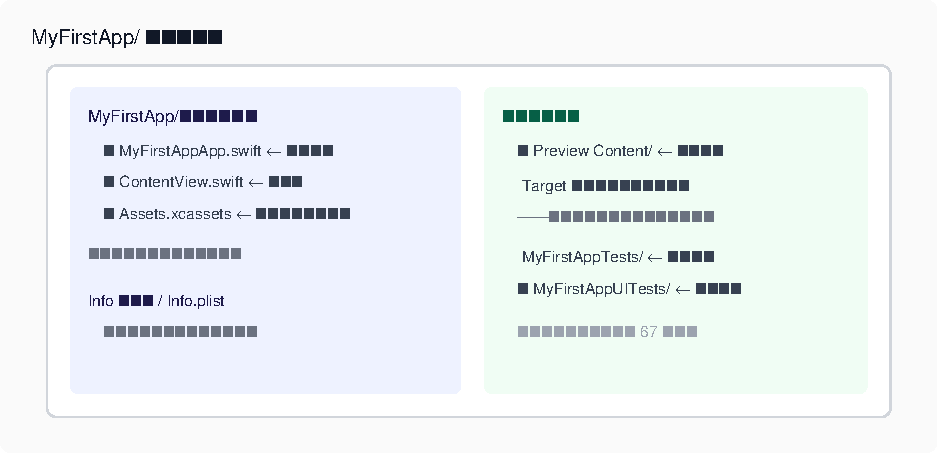
\includegraphics[width=0.92\linewidth]{figures/fig-di-liu-shi-zhang-1}
\\[2pt]\small 图 2：新手必懂的 Xcode 工程结构
\end{center}

\begin{itemize}
  \item \textbf{MyFirstAppApp.swift}：程序入口，SwiftUI 里它只有几行——"启动，然后显示主界面"；
  \item \textbf{ContentView.swift}：主界面视图，你现在看到的一切都在这里；
  \item \textbf{Assets.xcassets}：资源仓库——图标、图片、颜色都放这；
  \item \textbf{Target 设置}：点左侧蓝色工程图标进去，版本号、最低 iOS 版本、签名都在里面。App 显示名、图标也在这配置。
\end{itemize}

\booksection{五、真机调试：把 App 装进你的 iPhone}

\booksection{五、Xcode 效率技巧：新手的五个“快捷键外挂”}

用熟这几个，你会显得“很专业”：

\begin{center}
\begin{tabularx}{\linewidth}{|X|X|X|}
\hline
\textbf{操作} & \textbf{快捷键} & \textbf{作用} \tabularnewline
\hline
运行 & CmdR & 编译并跑起来 \tabularnewline
打开/切换画布预览 & OptionCmd & 所见即所得的开关 \tabularnewline
格式化缩进 & CtrlI & 自动整理选中代码的缩进 \tabularnewline
快速打开文件 & CmdO & 输入文件名秒开（最常用！） \tabularnewline
注释/取消注释 & Cmd/ & 调试时随手开关代码 \tabularnewline
\hline
\end{tabularx}
\end{center}

\begin{center}\small\color{gray}Xcode 高频快捷键（新手五件套）\end{center}

另外两个隐藏福利：\textbf{多开模拟器}（同时跑 iPhone 和 iPad 对比布局）和\textbf{代码片段库}（把常用的几行代码拖进右侧 Snippets 面板，下次一键插入）——效率工具先用起来，手感自然就上来了。

\booksection{六、真机调试：把 App 装进你的 iPhone}

模拟器虽好，真机才是终点。用免费 Apple ID 也能真机调试：

\begin{enumerate}
  \item 数据线连上 iPhone（或同 Wi-Fi 无线调试）；
  \item Xcode 顶部设备列表选你的手机，首次会提示登录 Apple ID 并自动配置签名；
  \item iPhone 上 [设置] [通用] [VPN与设备管理] 信任你的开发者证书；
  \item 点 >，App 装进真机。
\end{enumerate}

\begin{tcbwarn}{注意：免费账号的"七天限制"}
免费 Apple ID 签名的 App\textbf{7 天后会失效}（重新运行一次即可续期）。这是苹果的防滥用机制，学习阶段完全够用；付费开发者账号（99 美元/年）则没有这个限制，第 67 章细说。

\end{tcbwarn}

\booksection{七、小试牛刀 + 常见报错急救}

\booksection{六、小试牛刀 + 常见报错急救}

打开 ContentView.swift，把\texttt{Text(“Hello, world!”)}里的字换成你的名字，按CmdR重新运行——几秒后模拟器上就显示你的名字。恭喜，你完成了第一次完整的“改代码 编译 安装 运行”循环。

\begin{center}
\begin{tabularx}{\linewidth}{|X|X|X|}
\hline
\textbf{报错现象} & \textbf{常见原因} & \textbf{解药} \tabularnewline
\hline
Signing 报错 & Team 没选、证书过期 & Target Signing 里勾上你的账号；免费账号重跑一次 \tabularnewline
模拟器黑屏/打不开 & 镜像损坏 & 菜单 Device Erase All Content；或删掉重加模拟器 \tabularnewline
Xcode 下载慢/装不上 & App Store 网络波动 & 换时段；或到苹果开发者网站下载 .xip 离线包 \tabularnewline
\hline
\end{tabularx}
\end{center}

\begin{center}\small\color{gray}新手环境报错急救表\end{center}

\begin{tcbpractice}{来动手：完成你的"开发仪式感"清单}
(1) 装好 Xcode 并跑通模拟器；(2) 用真机跑一次自己的 App 并截图留念；(3) 把 Hello 文字改成你的名字；(4) 到 Target 设置里把 App 显示名改成“我的第一个App”。做完这四步，你就是有作品的人了。

\end{tcbpractice}

\begin{tcbsummary}{本章小结}
\begin{itemize}
  \item 硬门槛：Mac + Xcode；没有 Mac 先用 iPad 上的 Swift Playgrounds 学语言
  \item Xcode 从 App Store 装；新版本要求新系统，更新别拖
  \item 新建项目五要素：名字、Team、组织标识、SwiftUI、Swift
  \item 工程口诀：代码都在 MyFirstApp/ 目录；Target 设置管版本与签名
  \item 免费 Apple ID 真机调试有 7 天签名限制；付费账号无此限制
  \item 开发日常 = 改代码 CmdR 看效果，循环往复
\end{itemize}

\end{tcbsummary}

\bookchapter{第六十一章：Swift 快速上手——苹果开发的第一语言}

\chapterintro{这一章咱们正式学语言。别紧张——Swift 是出了名的“对新手友好”，而且你不需要背语法书：先掌握 20\% 的语法，就能看懂和写出 80\% 的日常代码。剩下的边做项目边查。记住咱们的学习原则：\textbf{看懂 > 记住，会用 > 精通}。}

\booksection{一、变量与类型：给数据起名字}

程序就是“数据 + 逻辑”。变量，就是给数据起个名字存起来。Swift 用\texttt{let}和\texttt{var}声明：

\begin{lstlisting}[language=Swift]
let name = "张三"        // let：常量（推荐默认用这个）
var age = 18             // var：变量（以后还能改）

age = 19                 // <i class="fas fa-check-circle mr-1"></i> var 可以改
// name = "李四"         // <i class="fas fa-times-circle mr-1"></i> let 不能改，编译报错

let score: Int = 100     // 也可以显式写明类型
let pi = 3.14            // 不写也能自动推断

print("你好，\(name)")   // 字符串插值：反斜杠 + 括号
\end{lstlisting}

常用类型一张表记住：

\begin{center}
\begin{tabularx}{\linewidth}{|X|X|X|}
\hline
\textbf{类型} & \textbf{存什么} & \textbf{示例} \tabularnewline
\hline
Int & 整数 & 42 \tabularnewline
Double & 小数 & 3.14 \tabularnewline
String & 文字 & "你好" \tabularnewline
Bool & 真/假 & true / false \tabularnewline
{}[Int]（数组） & 一组数据 & {}[1, 2, 3] \tabularnewline
\hline
\end{tabularx}
\end{center}

\begin{center}\small\color{gray}Swift 常用基础类型\end{center}

\begin{tcbinfo}{小贴士：let 优先原则}
Swift 社区的铁律：\textbf{默认用 let，确有必要再用 var}。能用 let 的地方用 var，Xcode 会黄字警告你。这个习惯能帮你少掉一大类“变量被意外修改”的 bug——代码越少变化，越容易推理。

\end{tcbinfo}

\booksection{二、可选值（Optional）：Swift 的“防崩护身符”}

这是 Swift 最重要的概念，没有之一。一句话：\textbf{一个值可能“不存在”时，Swift 强迫你处理它}——从语言层面消灭了“空指针崩溃”这个行业噩梦。

\begin{lstlisting}[language=Swift]
var name: String = "张三"   // 普通类型：绝不允许是 nil
// name = nil                // <i class="fas fa-times-circle mr-1"></i> 编译错误，直接拦住

var nickname: String? = nil  // 加个问号：允许为 nil（可选值）
nickname = "三儿"

// 使用可选值，必须"解包"：
if let n = nickname {        // if let：安全解包
    print("你好，\(n)")
} else {
    print("还没有昵称")
}

let len = nickname?.count ?? 0   // ?? 给默认值（空合运算符）
print(len)
\end{lstlisting}

\begin{tcbwarn}{注意：! 是"高危操作"}
代码里写\texttt{nickname!}（强制解包）等于对编译器喊“我保证它不是 nil”——一旦猜错，App 当场崩溃。新手期原则：\textbf{尽量用 if let / ?? ，不用 !}。Xcode 补全代码时偶尔会顺手加 !，记得改掉它。

\end{tcbwarn}

\booksection{三、函数与闭包：把逻辑打包成“按钮”}

函数是一段有名字的逻辑，像遥控器上的按钮。闭包（Closure）则是“没名字的函数”，可以随手递给别人：

\begin{lstlisting}[language=Swift]
// 函数：名字在前，参数和返回类型在后
func greet(name: String) -> String {
    return "你好，\(name)！"
}
print(greet(name: "张三"))     // 调用时要带参数名

// 闭包：就地定义，轻快直接
let numbers = [1, 2, 3, 4]
let doubled = numbers.map { $0 * 2 }   // $0 = 当前元素
// [2, 4, 6, 8]

let big = numbers.filter { $0 > 2 }    // 筛选
// [3, 4]
\end{lstlisting}

SwiftUI 里闭包无处不在：按钮的\texttt{Button(“点我”) \{ .\allowbreak .\allowbreak .\allowbreak  \}}后面的大括号就是一个闭包。\texttt{map}、\texttt{filter}、\texttt{sorted}这几个“集合连招”请记牢——未来 90\% 的列表处理都是它们的组合。

\booksection{四、结构体与协议：Swift 的“乐高”体系}

Swift 的官方偏好很明确：\textbf{优先用结构体（struct），需要继承时才用类（class）}。结构体是“值类型”——复制时各过各的，天然少一类 bug：

\begin{lstlisting}[language=Swift]
// 结构体：装数据的盒子
struct Record {
    var id = UUID()
    var amount: Double
    var category: String
    var date: Date

    // 结构体自带"成员逐一构造器"：直接就能创建
}
let r = Record(amount: 25.5, category: "餐饮", date: Date())

// 协议：约定"必须具备哪些能力"
protocol Identifiable {
    var id: UUID { get }
}
struct Record: Identifiable { ... }   // 遵守协议 = 承诺实现其要求
\end{lstlisting}

SwiftUI 里几乎一切都是 struct（View 就是协议）。这句现在不懂没关系，第 62 章会天天见面——\textbf{在 Swift 的世界里，先拥抱 struct}。

\booksection{五、写给零基础的语法速查卡}

\begin{center}
\begin{tabularx}{\linewidth}{|X|X|}
\hline
\textbf{要做什么} & \textbf{写法} \tabularnewline
\hline
定义常量/变量 & \texttt{let x = 1}/\texttt{var x = 1} \tabularnewline
字符串插值 & \texttt{"你好，\textbackslash{}(name)"} \tabularnewline
定义函数 & \texttt{func 名字(参数: 类型) -\allowbreak > 返回类型 \{ .\allowbreak .\allowbreak .\allowbreak  \}} \tabularnewline
判断 & \texttt{if 条件 \{ .\allowbreak .\allowbreak .\allowbreak  \} else \{ .\allowbreak .\allowbreak .\allowbreak  \}} \tabularnewline
遍历 & \texttt{for x in 数组 \{ .\allowbreak .\allowbreak .\allowbreak  \}} \tabularnewline
安全解包 & \texttt{if let x = 可选值 \{ .\allowbreak .\allowbreak .\allowbreak  \}} \tabularnewline
默认值 & \texttt{x ?? 默认值} \tabularnewline
定义结构体 & \texttt{struct X \{ var a: Int; var b: String \}} \tabularnewline
闭包 & \texttt{\{ \$0 * 2 \}} \tabularnewline
\hline
\end{tabularx}
\end{center}

\begin{center}\small\color{gray}Swift 语法速查卡（新手版）\end{center}

\begin{tcbpractice}{来动手：在 Playgrounds 里玩 15 分钟 Swift}
有 Mac 就打开 Xcode Playground；没 Mac 就用 iPad 上的 Swift Playgrounds 或网页版演练场。把本章每一段代码都跑一遍，改改数字和文字，故意制造几个错误看看 Xcode 怎么提示。这个“先玩后学”的 15 分钟，会让你第 62 章上手时轻松一倍。

\end{tcbpractice}

\begin{tcbsummary}{本章小结}
\begin{itemize}
  \item let 优先，var 慎用；类型自动推断，冒号后显式声明也行
  \item 可选值是 Swift 的灵魂：可能为空必须处理，if let / ?? 是护身符，! 是高危操作
  \item 函数调用要带参数名；闭包 = 没名字的函数，SwiftUI 里无处不在
  \item 优先 struct，遵守协议（Protocol）；SwiftUI 几乎一切都是 struct
  \item 20\% 语法干 80\% 的活：先会用，再精通
\end{itemize}

\end{tcbsummary}

\bookchapter{第六十二章：界面开发——SwiftUI 入门}

\chapterintro{界面是用户看到的一切。SwiftUI 是苹果 2019 年推出的\textbf{声明式}界面框架——你只需要“声明”界面长什么样，系统自动负责渲染、适配深色模式、适配各种屏幕。到 2026 年，SwiftUI 已是新项目的绝对主流。这一章，咱们学会“画画”。}

\booksection{一、SwiftUI 的思想：声明式，不是命令式}

老式界面开发是“命令式”：先告诉系统“创建按钮 放在(20,30) 设置颜色”，一步一步指挥。SwiftUI 是“声明式”：\textbf{你直接描述“界面上有一个红色按钮写着'点我'”}，怎么画、什么时候重画，系统自己操心。

\begin{lstlisting}[language=Swift]
import SwiftUI

struct ContentView: View {
    var body: some View {      // body：描述"界面长什么样"
        VStack {               // 竖着排列
            Text("你好，世界！")
                .font(.largeTitle)      // 修饰符：大标题
            Button("点我") {
                print("被点击了")
            }
            .buttonStyle(.borderedProminent)  // 蓝色实心按钮
        }
        .padding()
    }
}
\end{lstlisting}

关键点：\textbf{视图 = 遵守 View 协议的结构体}，\texttt{body}属性描述界面，\texttt{.\allowbreak 修饰符()}链式“上妆”。这就是 SwiftUI 的全部基本盘。

\booksection{二、基础视图：文字、按钮、输入框、图片}

\begin{center}
\begin{tabularx}{\linewidth}{|X|X|X|}
\hline
\textbf{视图} & \textbf{干什么} & \textbf{示例} \tabularnewline
\hline
Text & 显示文字 & \texttt{Text("你好")} \tabularnewline
Button & 按钮 & \texttt{Button("点我") \{ 动作 \}} \tabularnewline
TextField & 输入框 & \texttt{TextField("提示", text: \$文本)} \tabularnewline
Image & 显示图片 & \texttt{Image(systemName: "star.\allowbreak fill")} \tabularnewline
\hline
\end{tabularx}
\end{center}

\begin{center}\small\color{gray}SwiftUI 四大基础视图\end{center}

注意\texttt{Image(systemName:)}——苹果内置了\textbf{SF Symbols}图标库（几千个免费图标），“star.fill” 这种名字就能直接显示一个实心星星。这是 iOS 开发的隐藏福利：\textbf{做界面几乎不用找图标素材}。

\booksection{三、布局三件套：VStack、HStack、ZStack}

\begin{itemize}
  \item \textbf{VStack}：竖着排（像排队打饭）；
  \item \textbf{HStack}：横着排（像并排坐）；
  \item \textbf{ZStack}：叠着放（像扑克牌摞一起，适合做角标、遮罩）。
\end{itemize}

\begin{lstlisting}[language=Swift]
VStack(alignment: .leading, spacing: 12) {
    HStack {
        Text("账单")
        Spacer()                 // 弹性空间：把右边推到尽头
        Text("-25.5 元").foregroundColor(.red)
    }
    Divider()                    // 分割线
    Text("备注：午饭")
}
.padding(16)                     // 四周留白
.background(Color(.systemGray6)) // 浅灰底
.cornerRadius(12)                // 圆角

// 修饰符顺序有意义：先 padding 再 background，背景不含边距
\end{lstlisting}

\begin{tcbwarn}{注意：修饰符顺序有讲究}
\texttt{padding(16).\allowbreak background(灰)}和\texttt{background(灰).\allowbreak padding(16)}效果不同——前者“先留白再涂色”（背景不含边距），后者“先涂色再留白”（背景包含边距）。新手最常见的“奇怪白边”都源于此。不确定时调换顺序，预览立刻告诉你答案。

\end{tcbwarn}

\booksection{四、状态与绑定：让界面“活”起来}

静态界面没意思。SwiftUI 的规则：\textbf{界面永远忠实反映状态，状态变了，界面自动重画}。

\begin{lstlisting}[language=Swift]
struct CounterView: View {
    @State private var count = 0   // @State：这个值变了要重画

    var body: some View {
        VStack {
            Text("你点了 \(count) 次")
            Button("点我 +1") {
                count += 1          // 改状态，界面自动刷新
            }
        }
    }
}
\end{lstlisting}

输入框要用“双向绑定”——\texttt{\$}符号把“值和修改权”一起传进去：

\begin{lstlisting}[language=Swift]
struct InputView: View {
    @State private var text = ""

    var body: some View {
        TextField("输入点什么", text: $text)  // $ 双向绑定
            .textFieldStyle(.roundedBorder)
        Text("你输入了：\(text)")   // 输入时实时更新
    }
}
\end{lstlisting}

用户操作

状态改变（count += 1）

SwiftUI 感知到变化

自动重画界面（body 重新计算）

\begin{center}\small\color{gray}图 3：SwiftUI 的“状态 界面”单向数据流\end{center}

\booksection{五、预览、主题与动画：SwiftUI 的“外挂”}

\begin{itemize}
  \item \textbf{\#Preview 宏}：文件底部加\texttt{\#Preview \{ ContentView() \}}，右侧画布实时渲染——改代码所见即所得；
  \item \textbf{深色模式免费}：用系统颜色（\texttt{Color(.\allowbreak systemGray6)}、\texttt{.\allowbreak primary}）而不是写死颜色，深色模式自动适配，一行不用多写；
  \item \textbf{动画一行搞定}：\texttt{withAnimation \{ count += 1 \}}或给视图加\texttt{.\allowbreak animation(.\allowbreak default, value: count)}——过渡丝滑。
\end{itemize}

\begin{lstlisting}[language=Swift]
struct AnimatedHeartView: View {
    @State private var liked = false

    var body: some View {
        Button {
            withAnimation(.spring(duration: 0.4)) {
                liked.toggle()
            }
        } label: {
            Image(systemName: liked ? "heart.fill" : "heart")
                .font(.system(size: 48))
                .foregroundColor(liked ? .red : .gray)
                .scaleEffect(liked ? 1.3 : 1.0)
        }
    }
}
\end{lstlisting}

\begin{tcbinfo}{小贴士：先功能后动画}
新手常犯的毛病是“界面还没做对，就开始纠结动画”。先让功能跑通，最后再统一加动效——动画是锦上添花，功能是雪中送炭。这也是咱们一贯的“简单至上”原则。

\end{tcbinfo}

\begin{tcbpractice}{来动手：做一个"心情按钮"}
\booksection{六、常用修饰符速查：一页在手，界面不愁}

\begin{center}
\begin{tabularx}{\linewidth}{|X|X|}
\hline
\textbf{想做什么} & \textbf{修饰符} \tabularnewline
\hline
留白 & \texttt{.\allowbreak padding(16)} \tabularnewline
圆角 & \texttt{.\allowbreak cornerRadius(12)} \tabularnewline
背景色 & \texttt{.\allowbreak background(Color(.\allowbreak systemGray6))} \tabularnewline
字体与字号 & \texttt{.\allowbreak font(.\allowbreak title.\allowbreak bold())}/\texttt{.\allowbreak font(.\allowbreak system(size: 20))} \tabularnewline
前景色（文字/图标） & \texttt{.\allowbreak foregroundColor(.\allowbreak red)} \tabularnewline
撑满宽度 & \texttt{.\allowbreak frame(maxWidth: .\allowbreak infinity)} \tabularnewline
固定尺寸 & \texttt{.\allowbreak frame(width:100, height: 44)} \tabularnewline
对齐方式 & \texttt{VStack(alignment: .\allowbreak leading)} \tabularnewline
透明度 & \texttt{.\allowbreak opacity(0.\allowbreak 6)} \tabularnewline
阴影 & \texttt{.\allowbreak shadow(radius: 5)} \tabularnewline
点击手势 & \texttt{.\allowbreak onTapGesture \{ .\allowbreak .\allowbreak .\allowbreak  \}} \tabularnewline
键盘类型 & \texttt{.\allowbreak keyboardType(.\allowbreak decimalPad)} \tabularnewline
\hline
\end{tabularx}
\end{center}

\begin{center}\small\color{gray}SwiftUI 常用修饰符速查\end{center}

记不住没关系——这页就是用来查的。用得最多的其实就前四个：padding、圆角、背景、字体。

把模板项目改成一个心情切换器：一个按钮，点击后在 开心 难过 生气 之间循环切换，文字和背景色跟着变。提示：用数组存三组（文字+颜色），\texttt{@State}存下标，点击时\texttt{(index + 1) \% 3}。做完发给朋友玩，收获第一波“哇你会做 App 了”。

\end{tcbpractice}

\begin{tcbsummary}{本章小结}
\begin{itemize}
  \item SwiftUI 是声明式：描述"长什么样"，系统负责画和重画
  \item 视图 = 遵守 View 协议的结构体；body 描述界面；修饰符链式"上妆"
  \item 四大基础视图：Text / Button / TextField / Image；SF Symbols 图标库免费管饱
  \item 布局三件套：VStack 竖排、HStack 横排、ZStack 叠放；Spacer 是弹性空间
  \item @State 让界面活起来；\$ 双向绑定喂给输入框
  \item \#Preview 所见即所得；系统颜色自动适配深色模式；withAnimation 一行动效
\end{itemize}

\end{tcbsummary}

\bookchapter{第六十三章：视图、状态与导航}

\chapterintro{单页面的玩具已经会做了。这一章解决两个“长大”问题：怎么在多个页面之间跳来跳去（导航），以及数据在页面之间怎么流动（状态管理）。学完本章，你就能搭出“列表 详情 编辑”这种经典的多页面 App 骨架。}

\booksection{一、状态管理的“数据流全景”}

SwiftUI 的状态工具不止 @State 一个。先看这张全景图，搞懂“什么时候用哪个”：

\begin{center}
\begin{tabularx}{\linewidth}{|X|X|X|X|}
\hline
\textbf{工具} & \textbf{管什么} & \textbf{谁来用} & \textbf{典型场景} \tabularnewline
\hline
@State & 页面私有的临时状态 & 当前视图 & 计数器、输入框文字 \tabularnewline
@Binding & 借用别人的状态 & 子视图改父视图 & 自定义组件 \tabularnewline
@StateObject / @Observable & 跨页面共享的逻辑 & 视图模型（ViewModel） & 数据加载、业务逻辑 \tabularnewline
@EnvironmentObject / .environment & 全局共享的状态 & 整个 App & 用户登录态、主题设置 \tabularnewline
\hline
\end{tabularx}
\end{center}

\begin{center}\small\color{gray}SwiftUI 状态工具全景（2026 年，@Observable 已是主流）\end{center}

\begin{lstlisting}[language=Swift]
// iOS 17+ 的现代写法：@Observable 宏（推荐新项目使用）
import Observation

@Observable
class CounterModel {                 // 视图模型
    var count = 0
    func increment() { count += 1 }
}

struct CounterView: View {
    @State private var model = CounterModel()   // 持有模型

    var body: some View {
        VStack {
            Text("你点了 \(model.count) 次")
            Button("点我") { model.increment() }
        }
    }
}
\end{lstlisting}

给新手的粗暴建议：\textbf{页面私有的用 @State，跨页面/有逻辑的用 @Observable 类}。老教程里的 @StateObject/@ObservableObject 是上一代写法，能读懂即可，新代码按上面来。

\booksection{二、NavigationStack：页面跳转的“栈”}

iOS 16 起，多页面导航用\textbf{NavigationStack}——像一摞盘子，推一个进一个，返回时逐个弹出：

\begin{lstlisting}[language=Swift]
struct HomeView: View {
    var body: some View {
        NavigationStack {
            List {
                NavigationLink("张三的账本") {
                    DetailView(name: "张三的账本")   // 目标页面
                }
                NavigationLink("李四的账本") {
                    DetailView(name: "李四的账本")
                }
            }
            .navigationTitle("账本列表")   // 顶部大标题
        }
    }
}

struct DetailView: View {
    let name: String
    var body: some View {
        Text("\(name) 的详情页")
            .navigationTitle(name)
            .navigationBarTitleDisplayMode(.inline)
    }
}
\end{lstlisting}

NavigationLink 就是“能点的跳转链接”；\texttt{navigationTitle}自动生成导航栏标题和返回按钮。要\textbf{编程式跳转}（比如点完“保存”自动返回）时，用\texttt{@Environment(\textbackslash{}.\allowbreak dismiss)}关闭当前页面——这两招配合，90\% 的导航需求就齐了。

\booksection{三、弹窗与底部标签：sheet 与 TabView}

除了“推页面”，还有两种经典交互：

\begin{lstlisting}[language=Swift]
// 1. 底部弹出半屏/全屏（录入表单最爱）
struct HomeView: View {
    @State private var showAdd = false
    var body: some View {
        Button("记一笔") { showAdd = true }
            .sheet(isPresented: $showAdd) {
                AddRecordView()     // 弹出的录入页
            }
    }
}

// 2. 底部标签栏（App 的"骨架"）
struct MainTabView: View {
    var body: some View {
        TabView {
            RecordListView()
                .tabItem { Label("账本", systemImage: "book") }
            StatsView()
                .tabItem { Label("统计", systemImage: "chart.pie") }
            SettingsView()
                .tabItem { Label("设置", systemImage: "gear") }
        }
    }
}
\end{lstlisting}

\begin{tcbinfo}{小贴士：什么时候用哪种？}
经验法则：\textbf{主流程用 NavigationStack 推页面（列表详情），临时操作用 sheet 弹窗（新增、编辑、确认），并列的几大块用 TabView（底部标签）}。三者组合，就是绝大多数 App 的骨架。

\end{tcbinfo}

\booksection{四、List：iOS 的“国民列表”}

iOS 上最常用、最有“苹果味”的组件就是\textbf{List}——天然带分割线、滑动删除、点击高亮：

\begin{lstlisting}[language=Swift]
struct RecordListView: View {
    @State private var records = ["午饭 25.5", "地铁 6.0", "工资 +8000"]

    var body: some View {
        List {
            ForEach(records, id: \.self) { r in
                Text(r)
            }
            .onDelete { indexSet in          // 左滑删除
                records.remove(atOffsets: indexSet)
            }
        }
    }
}
\end{lstlisting}

列表 + NavigationLink + sheet + TabView——把这四样组合起来，你已经能搭出“账本列表 点开详情 点+弹录入”的完整 App 骨架了。下一章的记账本项目，就是这么搭的。

\begin{tcbpractice}{来动手：搭一个"三页骨架"}
\booksection{五、程序生命周期：前台与后台}

和安卓的 Activity 生命周期类似，iOS App 也有“出生、前台、后台、死亡”的状态变化。SwiftUI 里用\texttt{scenePhase}环境值观察：

\begin{lstlisting}[language=Swift]
@main
struct MyApp: App {
    @Environment(\.scenePhase) private var phase

    var body: some Scene {
        WindowGroup {
            ContentView()
        }
        .onChange(of: phase) { _, newPhase in
            switch newPhase {
            case .active:    print("回到前台，恢复刷新")
            case .inactive:  print("过渡中（来电/切后台瞬间）")
            case .background: print("进后台，保存草稿")
            @unknown default: break
            }
        }
    }
}
\end{lstlisting}

典型用途：\textbf{回前台时刷新数据，进后台时保存草稿}。iOS 对后台运行管得很严——普通 App 进后台后很快被挂起（冻结），别指望在后台偷偷干重活；真要定时任务，用第 68 章的本地通知，而不是“后台常驻”。

做一个假数据版本的记账本骨架：TabView 三个标签（账本/统计/设置） 账本页用 List 显示假数据、点行跳详情（NavigationStack） 右上角“+”按钮弹录入 sheet。不存数据、不联网，纯练骨架——这个骨架做好，第 65 章往里填真数据就是水到渠成。

\end{tcbpractice}

\begin{tcbsummary}{本章小结}
\begin{itemize}
  \item 状态四工具：@State（页面私有）、@Binding（借用）、@Observable（逻辑）、.environment（全局）
  \item 新项目用 @Observable 宏写视图模型；老教程的 @ObservableObject 能读即可
  \item NavigationStack 推页面；@Environment(\textbackslash{}.dismiss) 编程式返回
  \item 主流程推页面、临时操作弹 sheet、并列大块用 TabView
  \item List 是"国民列表"：分割线、滑动删除开箱即用
\end{itemize}

\end{tcbsummary}

\bookchapter{第六十四章：数据存储与网络请求}

\chapterintro{一个只能“看”的 App 是死的；能存数据、能连网络的 App 才是活的。这一章认识 iOS 数据层的“三件套”：UserDefaults（存小配置）、SwiftData（存结构化数据）、URLSession（和服务器对话），外加解析 JSON 的 Codable 和现代化的 async/await。学完这章，你就能写会记住用户习惯、会实时更新内容的真 App 了。}

\booksection{一、存储方案怎么选：先看这张表}

\begin{center}
\begin{tabularx}{\linewidth}{|X|X|X|X|}
\hline
\textbf{方案} & \textbf{适合存什么} & \textbf{特点} & \textbf{本书哪里用} \tabularnewline
\hline
UserDefaults & 零散配置（开关、偏好） & 键值对，简单直接 & 第 65 章设置、第 66 章收藏城市 \tabularnewline
SwiftData & 结构化数据（账目、记录） & 官方数据库封装，@Model 一行声明 & 第 65 章账目记录 \tabularnewline
URLSession & （不存，联网取）服务器数据 & 系统自带网络框架，无第三方依赖 & 第 66 章天气数据 \tabularnewline
\hline
\end{tabularx}
\end{center}

\begin{center}\small\color{gray}数据三件套的分工\end{center}

记一个口诀：\textbf{“小配置进 UserDefaults，成批数据进 SwiftData，外面的数据走 URLSession”}。旧教程里的 Core Data 依然能用（SwiftData 就是它的现代马甲），手写 SQLite 则基本不用碰——直接学新的，别走老路。

\booksection{二、UserDefaults：存点小配置}

\begin{lstlisting}[language=Swift]
// 写：存一个值
UserDefaults.standard.set(true, forKey: "isDarkMode")
UserDefaults.standard.set("北京", forKey: "favoriteCity")

// 读：取出来（没有就返回默认值）
let isDark = UserDefaults.standard.bool(forKey: "isDarkMode")
let city = UserDefaults.standard.string(forKey: "favoriteCity") ?? "北京"

// 删：移除一个键
UserDefaults.standard.removeObject(forKey: "isDarkMode")
\end{lstlisting}

注意它只适合\textbf{零散的小配置}——几十上百条记录请交给 SwiftData，别把 UserDefaults 当数据库用（会拖慢启动、也不便查询）。

\booksection{三、SwiftData：给数据安个“真正的家”}

SwiftData 是 iOS 17 起的官方数据库方案，把“建表、增删改查”简化到了极致——\textbf{一个 @Model 注解，数据类就变成数据库表}：

\begin{lstlisting}[language=Swift]
import SwiftData

// 1. @Model：这个类自动变成"表"
@Model
class Record {
    var amount: Double
    var category: String
    var note: String
    var date: Date

    init(amount: Double, category: String, note: String, date: Date) {
        self.amount = amount
        self.category = category
        self.note = note
        self.date = date
    }
}

// 2. App 入口挂上容器
@main
struct MyApp: App {
    var body: some Scene {
        WindowGroup {
            ContentView()
        }
        .modelContainer(for: Record.self)   // 数据库就绪
    }
}

// 3. 视图里用 @Query 读、@Environment 写
struct RecordListView: View {
    @Query(sort: \Record.date, order: .reverse) var records: [Record]
    @Environment(\.modelContext) private var context

    var body: some View {
        List(records) { r in
            Text("\(r.category) \(r.amount) 元")
        }
    }

    func add(amount: Double, category: String) {
        let r = Record(amount: amount, category: category, note: "", date: Date())
        context.insert(r)     // 存
        try? context.save()   // 落盘
    }
}
\end{lstlisting}

这套“@Model + modelContainer + @Query”模板可以原样搬进你的任何项目——换换字段名就行。数据一变，@Query 自动刷新界面，妙不可言。

\booksection{四、Codable：给 JSON“翻译”}

服务器的数据大多是 JSON 文本。Swift 的\textbf{Codable}协议让“JSON 结构体”的转换自动发生——字段名对得上，魔法就生效：

\begin{lstlisting}[language=Swift]
// JSON: {"name":"北京","main":{"temp":26.5},"weather":[{"description":"晴"}]}
struct WeatherResponse: Codable {
    let name: String
    let main: Main
    let weather: [Weather]
}
struct Main: Codable { let temp: Double }
struct Weather: Codable { let description: String }

// JSON 字符串  结构体
let decoder = JSONDecoder()
let data = jsonString.data(using: .utf8)!
let result = try decoder.decode(WeatherResponse.self, from: data)
print(result.weather[0].description)   // "晴"
\end{lstlisting}

铁律：\textbf{先看真实返回的 JSON，再定义字段}。很多“解析失败”的 bug 都是字段名写错、类型猜错（服务器发 “26.5” 字符串，你声明成 Double）——把原始 JSON 打印出来对照，十秒定位。

\booksection{五、URLSession + async/await：和服务器说话}

iOS 联网用系统自带的\textbf{URLSession}，配合 Swift 的\textbf{async/await}（异步函数），“等网络”就像“等快递”一样自然：

\begin{lstlisting}[language=Swift]
struct WeatherService {
    // 异步函数：async 标记"我要等一会儿"，throws 标记"可能失败"
    func fetchWeather(city: String) async throws -> WeatherResponse {
        let url = URL(string:
            "https://api.example.com/weather?city=\(city)")!
        let (data, _) = try await URLSession.shared.data(from: url)
        return try JSONDecoder().decode(WeatherResponse.self, from: data)
    }
}

// 调用处（在 .task 里）：
.task {
    do {
        let weather = try await service.fetchWeather(city: "北京")
        // 更新界面……
    } catch {
        print("出错了：\(error)")
    }
}
\end{lstlisting}

\textbf{避坑提醒：两条网络铁律}\par

(1)\textbf{联网必须 async/await，绝不阻塞主线程}——卡住界面是崩溃级体验。Swift 的结构化并发让这变得很自然，但别忘了\texttt{try await}和\texttt{do/catch}。(2)\textbf{ATS 默认禁止明文 HTTP}：iOS 要求 HTTPS。测试本地 http:// 服务时需要在 Info.plist 里临时开例外（NSAppTransportSecurity），但正式产品必须全走 HTTPS——审核也会盯这个。

\begin{tcbpractice}{来动手：做一个"每日一句"小应用}
\booksection{六、网络错误也要“分级”：别把一切报错都丢给用户}

断网、超时、404、服务器 500……不同的错，用户该看到的话不一样：

\begin{lstlisting}[language=Swift]
func friendlyMessage(_ error: Error) -> String {
    if let urlError = error as? URLError {
        switch urlError.code {
        case .notConnectedToInternet: return "网络断了，检查一下连接？"
        case .timedOut:               return "请求超时，稍后再试？"
        case .cannotFindHost:         return "服务器找不到了"
        default:                      return "网络出问题了：\(urlError.code)"
        }
    }
    if let d = error as? DecodingError {
        return "数据格式不对（可能是接口变了）"
    }
    return "出错了：\(error.localizedDescription)"
}
\end{lstlisting}

给用户看“人话”，给日志看“原话”（print 完整 error）。别把\texttt{error.localizedDescription}的英文天书直接甩给用户——产品感就藏在这些细节里。

找一个免费的名言 API（比如 hitokoto 之类），用 URLSession + async/await 拉取“每日一句”，显示在屏幕中央，加个“换一句”按钮。再把喜欢的句子用 SwiftData 存进“收藏夹”。这个练习把 UserDefaults/SwiftData/Codable/URLSession 全用了一遍——做完它，第 7、8 章就是小菜一碟。

\end{tcbpractice}

\begin{tcbsummary}{本章小结}
\begin{itemize}
  \item 口诀：小配置进 UserDefaults，成批数据进 SwiftData，外面的数据走 URLSession
  \item SwiftData 三板斧：@Model 声明表、modelContainer 挂容器、@Query 读 + context.insert 写
  \item Codable 自动"翻译" JSON：字段对得上，魔法就生效
  \item URLSession + async/await：联网像等快递；do/catch 处理失败
  \item 两条铁律：不阻塞主线程；正式产品必须 HTTPS（ATS）
\end{itemize}

\end{tcbsummary}

\bookchapter{第六十五章：项目一——我的记账本（本地版）}

\chapterintro{欢迎来到你的第一个“正经项目”。这个记账本虽然不联网，但五脏俱全：能记一笔账、能看流水、能按月统计、能删改。做完它，你就完整走了一遍“数据 逻辑 界面”的全流程。别急着抄代码——\textbf{先想清楚再动手}，这是咱们一贯的原则。}

\booksection{一、需求思考：先问五个问题}

\begin{center}
\begin{tabularx}{\linewidth}{|X|X|}
\hline
\textbf{要素} & \textbf{答案} \tabularnewline
\hline
Who（给谁用） & 自己用，家人朋友也行 \tabularnewline
What（做什么） & 记收支、看流水、按月汇总、按分类统计 \tabularnewline
Why（为什么） & 练手 + 搞清楚钱花哪儿了 \tabularnewline
How（怎么做） & Swift + SwiftUI + SwiftData + MVVM，纯本地无后端 \tabularnewline
Constraint（约束） & 一周内完成；最低支持 iOS 17（SwiftData 门槛） \tabularnewline
\hline
\end{tabularx}
\end{center}

\begin{center}\small\color{gray}记账本需求五要素\end{center}

然后拆解成“每一步都能用”的小步骤：(1) 建 SwiftData 数据层（能存一笔账）；(2) 列表页（能看流水）；(3) 录入弹窗（能加账）；(4) 删除与编辑；(5) 月度汇总卡片。每完成一步，App 都是一个“能用的东西”。

\booksection{二、数据层：让“账”有个家}

先定义一笔账长什么样——字段要够用但别贪多：

\begin{lstlisting}[language=Swift]
import SwiftData

@Model
class Record {
    var type: String      // "income" 收入 | "expense" 支出
    var amount: Double    // 金额（元）
    var category: String  // 分类：餐饮、交通、工资……
    var note: String      // 备注（可选）
    var date: Date        // 记账日期

    init(type: String, amount: Double, category: String, note: String = "", date: Date = Date()) {
        self.type = type
        self.amount = amount
        self.category = category
        self.note = note
        self.date = date
    }
}
\end{lstlisting}

\begin{tcbinfo}{小贴士：金额为什么用 Double？}
严谨的金融 App 会用 Decimal（精确十进制）来避免浮点误差（0.1+0.2$\neq$0.3 的老问题）。练手项目用 Double 足够；如果哪天做真金融产品，记得换成\texttt{Decimal}或“以分为单位的 Int”——这是无数前辈踩出来的坑。

\end{tcbinfo}

\booksection{三、MVVM：界面与逻辑“分家”}

直接让界面操作数据库？能跑，但界面代码会又臭又长。MVVM 架构让各司其职：\textbf{View（界面）只管画，ViewModel（逻辑中枢）管数据，Model（SwiftData）管存储}。

View（SwiftUI 界面）

ViewModel（@Observable 逻辑中枢）

Model（SwiftData 数据层）

\begin{center}\small\color{gray}图 4：MVVM 三层结构——数据单向流动，各层互不越界\end{center}

\begin{lstlisting}[language=Swift]
import Observation

@Observable
class RecordViewModel {
    var records: [Record] = []
    private let context: ModelContext

    init(context: ModelContext) { self.context = context }

    func load() {
        // SwiftData 的 #Predicate 筛选 + 排序
        let descriptor = FetchDescriptor<Record>(
            sortBy: [SortDescriptor(\.date, order: .reverse)]
        )
        records = (try? context.fetch(descriptor)) ?? []
    }

    func add(type: String, amount: Double, category: String, note: String) {
        let r = Record(type: type, amount: amount, category: category, note: note)
        context.insert(r)
        try? context.save()
        load()                       // 重新加载，界面刷新
    }

    func delete(_ record: Record) {
        context.delete(record)
        try? context.save()
        load()
    }
}
\end{lstlisting}

界面里\texttt{@State private var vm = RecordViewModel(.\allowbreak .\allowbreak .\allowbreak )}，然后直接\texttt{vm.\allowbreak records}渲染列表——数据一变，界面自动刷新。

\booksection{四、界面：列表页 + 录入弹窗}

\begin{lstlisting}[language=Swift]
struct RecordListView: View {
    @State private var vm: RecordViewModel
    @State private var showAdd = false

    var body: some View {
        NavigationStack {
            List {
                Section("本月结余") {          // 汇总卡片
                    SummaryRow(records: vm.records)
                }
                Section("流水") {
                    ForEach(vm.records) { r in
                        RecordRow(record: r)
                    }
                    .onDelete { idx in
                        idx.forEach { vm.delete(vm.records[$0]) }
                    }
                }
            }
            .navigationTitle("我的记账本")
            .toolbar {
                Button { showAdd = true } label: {
                    Image(systemName: "plus")
                }
            }
            .sheet(isPresented: $showAdd) {
                AddRecordView(vm: vm)          // 录入弹窗
            }
        }
    }
}
\end{lstlisting}

录入弹窗要点：金额输入框键盘用\texttt{.\allowbreak keyboardType(.\allowbreak decimalPad)}（数字键盘），收入/支出用分段控件（Picker），分类用菜单选择，点“保存”调\texttt{vm.\allowbreak add(.\allowbreak .\allowbreak .\allowbreak )}并\texttt{dismiss()}关窗。

\begin{tcbwarn}{注意：输入校验别偷懒}
金额输入框一定要校验：空值、负数、“abc”这类非法输入都要拦住（用\texttt{Double(text)}判断，失败返回 nil）。App 崩掉最常见的原因之一就是“把用户的输入当成了乖孩子”。记住：\textbf{用户输入的一切，都要当敌人审查}。

\end{tcbwarn}

\booksection{五、编辑、删除与汇总}

\begin{itemize}
  \item \textbf{删除}：List 的 .onDelete 左滑删除 + 确认弹窗（误删是记账类 App 用户最痛恨的事）；
  \item \textbf{编辑}：点行进编辑弹窗，预填原值（改一个字比重新输入省事）；
  \item \textbf{汇总}：用\texttt{filter}+\texttt{reduce}算"本月收入 / 支出 / 结余"，顶部卡片展示：
\end{itemize}

\begin{lstlisting}[language=Swift]
func monthSummary(_ records: [Record]) -> (income: Double, expense: Double) {
    let cal = Calendar.current
    let monthRecords = records.filter {
        cal.isDate($0.date, equalTo: Date(), toGranularity: .month)
    }
    let income = monthRecords
        .filter { $0.type == "income" }
        .reduce(0) { $0 + $1.amount }
    let expense = monthRecords
        .filter { $0.type == "expense" }
        .reduce(0) { $0 + $1.amount }
    return (income, expense)
}
\end{lstlisting}

\booksection{六、验收：三层检查 + 两个进阶挑战}

项目做完，按“功能 边界 架构”三层验收：能不能记、能不能删、重启 App 数据还在不在（功能）；金额输 0 或负数会不会崩（边界）；界面和数据有没有混在一起、字段有没有硬编码（架构）。

基础版验收通过后，给自己加两道“进阶菜”：

\begin{enumerate}
  \item \textbf{分类统计}：加一个"统计"标签页，用\textbf{Swift Charts}把分类支出画成饼图/柱状图——苹果官方图表库，几行代码出图；
  \item \textbf{iCloud 同步}：SwiftData 开 iCloud 同步只需配几项设置——账本在 iPhone/iPad 之间自动同步，瞬间"高级"起来。
\end{enumerate}

\begin{tcbpractice}{来动手：本周完成它}
按“数据层 ViewModel 列表页 录入弹窗 汇总卡片”的顺序动手，每天一步。卡住了就把报错原样丢给搜索引擎或 AI（还记得第七篇《AI编程实战篇》吗？描述问题时说清“期望行为、实际行为、复现步骤”）。完成后用它记一周账——自己做的 App 用起来，成就感会推着你继续往前走。

\end{tcbpractice}

\begin{tcbsummary}{本章小结}
\begin{itemize}
  \item 需求五要素 拆成"每步能用"的小步骤，再动手
  \item 数据层：@Model 模型 + modelContainer 容器 + FetchDescriptor 查询
  \item MVVM 分工：View 只管画，@Observable 的 ViewModel 管逻辑，SwiftData 管存储
  \item 界面：List + Section + toolbar + sheet 录入弹窗
  \item 三层验收（功能/边界/架构）+ 进阶挑战（Swift Charts、iCloud 同步）
\end{itemize}

\end{tcbsummary}

\bookchapter{第六十六章：项目二——天气查询 App（网络版）}

\chapterintro{记账本是“练内功”，天气 App 是“见世面”——它要和互联网打交道。这个项目你会学到：申请免费 API、解析 JSON、处理“加载中/成功/失败”三种界面状态，以及怎么把 API 密钥藏好。做完它，你就具备了做任何“联网 App”的能力——新闻、汇率、翻译，套路一模一样。}

\booksection{一、申请免费天气 API}

个人练手，推荐\textbf{OpenWeatherMap}或国内的\textbf{和风天气（QWeather）}——都有免费额度，注册即用。以 OpenWeatherMap 为例：

\begin{enumerate}
  \item 注册账号 在 API keys 页面生成一个 Key（\texttt{apikey}）；
  \item 免费版可调用 Current Weather 接口：\texttt{api.openweathermap.org/data/2.5/weather?q=beijing\&appid=你的Key\&units=metric}；
  \item 浏览器里先试一次，看看返回的 JSON 长什么样——这是接任何 API 前必做的"预习"。
\end{enumerate}

\textbf{避坑提醒：密钥绝不能写死在代码里}\par

API Key 相当于你的“钱包密码”，写进代码一提交到 GitHub，几小时内就会被爬虫扫走盗刷。iOS 的正确做法：放进\texttt{Config.xcconfig}（配置文件，已被 gitignore 忽略），通过 Info.plist 读入代码。搜索“iOS xcconfig 管理密钥”照着改即可。

\booksection{二、网络层：URLSession + Codable}

先照 API 返回的 JSON 定义模型，再写服务：

\begin{lstlisting}[language=Swift]
// JSON: {"weather":[{"description":"晴"}],"main":{"temp":26.5,"humidity":40},"name":"北京"}
struct WeatherResponse: Codable {
    let weather: [Weather]
    let main: Main
    let name: String
}
struct Weather: Codable { let description: String }
struct Main: Codable { let temp: Double; let humidity: Int }

struct WeatherService {
    let key: String   // 从 xcconfig 读入

    func fetchWeather(city: String) async throws -> WeatherResponse {
        var comps = URLComponents(string: "https://api.openweathermap.org/data/2.5/weather")!
        comps.queryItems = [
            URLQueryItem(name: "q", value: city),
            URLQueryItem(name: "appid", value: key),
            URLQueryItem(name: "units", value: "metric"),
            URLQueryItem(name: "lang", value: "zh_cn")
        ]
        let (data, _) = try await URLSession.shared.data(from: comps.url!)
        return try JSONDecoder().decode(WeatherResponse.self, from: data)
    }
}
\end{lstlisting}

\booksection{三、三种界面状态：加载中 / 成功 / 失败}

联网 App 的灵魂在于“状态管理”。网络慢、断网、城市名打错……每种情况界面都要给用户交代。用\textbf{枚举 + switch}优雅地表示：

\begin{lstlisting}[language=Swift]
enum LoadState {
    case loading                  // 转圈中
    case success(WeatherResponse) // 成功
    case error(String)            // 失败
}

@Observable
class WeatherViewModel {
    var state: LoadState = .loading
    private let service = WeatherService(key: Config.apiKey)

    func search(city: String) async {
        state = .loading
        do {
            let data = try await service.fetchWeather(city: city)
            state = .success(data)
        } catch {
            state = .error("查不到这个城市，换个名字试试？")
        }
    }
}

// 界面里：
switch vm.state {
case .loading: ProgressView("加载中…")
case .success(let d): WeatherContent(data: d)
case .error(let msg): Text(msg).foregroundColor(.secondary)
}
\end{lstlisting}

这个\texttt{loading/success/error}三段式是联网界面的“万金油模板”，先背下来，以后所有联网 App 照葫芦画瓢。

\booksection{四、实战界面代码：把天气画出来}

\begin{lstlisting}[language=Swift]
struct WeatherContent: View {
    let data: WeatherResponse

    var body: some View {
        VStack(spacing: 12) {
            Text(data.name)
                .font(.title.bold())
            Text("\(Int(data.main.temp))°C")
                .font(.system(size: 76, weight: .thin))
            Text(data.weather.first?.description ?? "未知")
                .font(.title3)
                .foregroundColor(.secondary)
            HStack(spacing: 24) {
                Label("湿度 \(data.main.humidity)%", systemImage: "humidity")
                Label("体感 \(Int(data.main.temp))°C", systemImage: "thermometer")
            }
        }
        .padding()
    }
}
\end{lstlisting}

几个小细节值得学：\texttt{first?}安全取第一个元素（列表可能为空），\texttt{?? “未知”}给兜底文案；76 号细字重的温度数字是天气类 App 的经典配方；\texttt{Label}是“图标+文字”的官方组件，比手拼 HStack 更规范。

\booksection{五、交互细节与收藏城市}

\begin{itemize}
  \item \textbf{搜索框}：顶部\texttt{.searchable}修饰符，系统自带搜索交互，提交时调\texttt{vm.search}；
  \item \textbf{收藏城市}：把常看的城市存进 UserDefaults，下次打开自动查；
  \item \textbf{下拉刷新}：\texttt{.refreshable \{ await vm.search(...) \}}一行搞定；
  \item \textbf{天气图标}：用\texttt{Image(systemName:)}按描述映射（sun.max / cloud.rain / snowflake），界面立刻活起来。
\end{itemize}

\begin{tcbinfo}{小贴士：中文城市的"梗"}
OpenWeatherMap 对中文城市名支持一般，搜“北京”可能无结果而 “beijing” 正常。产品化做法是内置一份“城市名 英文/坐标”映射表，或接国内天气服务。练手阶段先支持拼音/英文城市名即可，别和它较劲。

\end{tcbinfo}

\begin{tcbpractice}{来动手：天气 App 验收清单}
\booksection{六、网络请求怎么调试：打印、抓包与模拟慢网}

联网 App 出问题，十有八九在“请求没发对”或“响应没解析对”。三个调试手段：

\begin{enumerate}
  \item \textbf{打印原始数据}：把\texttt{String(data: data, encoding: .utf8)}打印出来看原始 JSON——字段名、类型一目了然，比猜快十倍；
  \item \textbf{抓包工具}：Mac 上免费的 Proxyman / 开源 Charles 能截获 App 的全部请求和响应，像 X 光一样看清网络层；
  \item \textbf{模拟弱网}：模拟器菜单 Features Network Link Conditioner（需从开发者网站下载工具），能模拟 3G、高延迟——测出"转圈半天"的体验问题。
\end{enumerate}

\begin{tcbinfo}{小贴士：请求没过 ATS？}
如果请求一发出就报 “App Transport Security” 错误，八成是用了 http:// 明文地址。正式接口必须 HTTPS；本地调试临时开例外（Info.plist 加 NSAllowsLocalNetworking），上架前记得清干净。

\end{tcbinfo}

(1) 正常搜索出天气；(2) 断开网络，App 优雅报错不崩溃（模拟器里关掉 Mac 的网络测！）；(3) 输一个不存在的城市，提示友好；(4) 收藏两个城市，重启 App 还在；(5) 深色模式下界面不刺眼。五条全过，这个项目才算毕业。

\end{tcbpractice}

\begin{tcbsummary}{本章小结}
\begin{itemize}
  \item 先浏览器试 API、看懂 JSON，再写代码——"预习"永远不亏
  \item API Key 藏进 xcconfig，绝不进代码库
  \item Codable 模型 + URLSession async/await：字段对上，JSON 自动解析
  \item loading/success/error 三段式状态是联网界面万金油
  \item 断网、空输入、城市不存在——错误处理是联网 App 的及格线
\end{itemize}

\end{tcbsummary}

\bookchapter{第六十七章：打磨与发布——测试、调试与上架 App Store}

\chapterintro{App 做出来了，然后呢？这一章回答“从能跑”到“能交付”的三件事：怎么高效地调试找 bug、怎么写测试防回归、怎么把 App 送上 App Store 让全世界下载。上架不只是仪式感——它是把一个作品变成产品的分水岭。}

\booksection{一、调试三板斧：print、断点、预览}

\begin{center}
\begin{tabularx}{\linewidth}{|X|X|X|}
\hline
\textbf{工具} & \textbf{干什么} & \textbf{怎么用} \tabularnewline
\hline
print + 控制台 & 看运行日志 & 代码里 print("值=\textbackslash{}(x)")，Xcode 底部控制台看输出 \tabularnewline
断点调试 & 让程序停在某行，看变量值 & 行号旁点一下出蓝标，运行到那里暂停，逐步走 \tabularnewline
SwiftUI 预览 + 调试器 & 实时看界面与视图层级 & \#Preview 画布 + 运行时的 View Hierarchy 检查器 \tabularnewline
\hline
\end{tabularx}
\end{center}

\begin{center}\small\color{gray}调试三板斧\end{center}

\begin{tcbinfo}{小贴士：崩溃了怎么读？}
Swift 崩溃时控制台会打印 “Fatal error” 加原因，Xcode 会停在出错那一行并高亮。真机上的历史崩溃可以在 Xcode Window Organizer Crashes 里看（需付费账号）。关键词优先搜\textbf{“错误原因第一句 + swiftui”}——精确的问题，才有精确的答案。

\end{tcbinfo}

\booksection{二、测试：给代码上保险}

手测靠不住——改了这个功能，另一个悄悄坏了。测试就是“后悔药”兼“防弹衣”。iOS 用\textbf{XCTest}框架，分两种：

\begin{center}
\begin{tabularx}{\linewidth}{|X|X|X|X|}
\hline
\textbf{层级} & \textbf{测什么} & \textbf{Target} & \textbf{速度} \tabularnewline
\hline
单元测试 & 纯逻辑（计算、校验） & MyFirstAppTests & 秒级 \tabularnewline
UI 测试 & 真实界面行为 & MyFirstAppUITests & 分钟级 \tabularnewline
手动测试 & 真人感受、体验 & —— & 永远需要 \tabularnewline
\hline
\end{tabularx}
\end{center}

\begin{center}\small\color{gray}iOS 测试层级（模板项目已预置两个 Test Target）\end{center}

\begin{lstlisting}[language=Swift]
import XCTest

// 把"金额字符串转数字"这种逻辑抽成纯函数
func parseAmount(_ input: String) -> Double? {
    guard let v = Double(input.trimmingCharacters(in: .whitespaces)),
          v > 0 else { return nil }
    return v
}

final class AmountTests: XCTestCase {
    func testEmptyInputReturnsNil() {
        XCTAssertNil(parseAmount(""))
    }
    func testNegativeReturnsNil() {
        XCTAssertNil(parseAmount("-5"))
    }
    func testNormalValueParses() {
        XCTAssertEqual(parseAmount("12.5"), 12.5)
    }
}
\end{lstlisting}

跑测试：CmdU。全绿之后再改代码，心里有底。记账本里的金额校验、汇总计算，都该有单元测试罩着。

\booksection{三、签名与打包：给 App 盖上“印章”}

每个 iOS App 都必须\textbf{签名}才能安装——证明“这个包出自你，没被篡改”。层级关系：

\begin{itemize}
  \item \textbf{学习阶段}：免费 Apple ID + Xcode 自动签名（Personal Team），真机可跑，7 天续期一次；
  \item \textbf{分发阶段}：付费开发者账号（99 美元/年）签发证书与描述文件，才能上架和长期安装。
\end{itemize}

打包：Xcode 菜单 Product Archive（归档），构建完成后在 Organizer 里Distribute App选 App Store Connect 上传。\textbf{归档必须用 Generic iOS Device 作为目标}（不是模拟器），这是新手常忘的一步。

\textbf{避坑提醒：证书丢了 = 更新断档}\par

签名证书和私钥一旦丢失，你无法再给旧 App 发更新——用户只能装“全新”应用。妥善备份证书（钥匙串导出 .p12）并记好密码。好在苹果提供了“自动签名”和云证书管理（Xcode 里勾选 Automatically manage signing），能省掉大部分手工操作的坑。

\booksection{四、上架 App Store 全流程}

注册开发者账号

准备商店素材

上传构建包

填隐私与审核信息

苹果审核（1-7 天）

上架

\begin{center}\small\color{gray}图 5：App Store 上架六步走\end{center}

\begin{itemize}
  \item \textbf{注册}：developer.apple.com，个人账号 99 美元/年；
  \item \textbf{素材}：图标（1024×1024，别带圆角——苹果自己切）、截图（iPhone 各尺寸）、描述、隐私政策链接；
  \item \textbf{隐私问卷}：如实申报收集了哪些数据——不联网的记账本可以"不收集任何数据"；
  \item \textbf{审核}：首次提交常有 1-7 天等待，被拒就按"审核备注"逐条改——苹果的拒绝理由通常写得非常具体，照做即可；
  \item \textbf{TestFlight}：上架前先把测试版发给朋友内测（最多 10000 人），收集一轮反馈再正式提交，专业范儿十足。
\end{itemize}

\booksection{五、商店素材怎么做：第一印象就是下载量}

商店页是用户“逛店”时看到的橱窗。三个素材决定第一印象：

\begin{itemize}
  \item \textbf{图标}：1024×1024，别用截图凑合。没设计能力就用 AI 工具生成一个简洁图形，\textbf{在桌面上缩小后还能一眼认出}才算合格；
  \item \textbf{截图}：至少 2 套（iPhone 主流尺寸），展示最核心的功能场景；每张配一句人话文案（"一秒记一笔"比"高效的记账解决方案"好十倍）；
  \item \textbf{描述}：第一句说清"这是什么 + 给谁用"，别堆砌"最专业、最强"——真诚比夸张有效。
\end{itemize}

\begin{tcbpractice}{来动手：把记账本"交付"一次}
\booksection{六、崩溃上报与性能优化小清单}

App 上架前，这两件事值得各花半小时：

\booksubsection{崩溃监控}

你测试时没崩，不代表用户手机不崩。苹果在 Xcode Organizer 里提供免费的崩溃报告（付费账号可看真机崩溃日志）；更省心的方案是接入第三方 SDK（如 Firebase Crashlytics）。\textbf{没有崩溃监控的上架，等于闭着眼睛开车}。

\booksubsection{性能自查四条}

\begin{enumerate}
  \item \textbf{列表用 LazyVStack / List}：长列表别用普通 VStack 硬排——懒加载是性能第一课；
  \item \textbf{图片别硬塞原图}：用 AsyncImage（远程图）和系统缓存，5MB 原图足以卡爆老机型；
  \item \textbf{别在主线程干重活}：网络、大文件都走 async/await；
  \item \textbf{用 Instruments 量一量}：Xcode 自带的性能分析器（Time Profiler、内存泄漏检查）——先测量，再优化，别凭感觉。
\end{enumerate}

(1) 给 parseAmount 等逻辑补 3 个单元测试（CmdU 跑绿）；(2) 用断点亲手抓一个自己制造的崩溃并修好；(3) Product Archive 打一个包，走 TestFlight 邀请朋友内测；(4) 有余力就注册开发者账号，把记账本真正提交上架。前三步今晚就能做完。

\end{tcbpractice}

\begin{tcbsummary}{本章小结}
\begin{itemize}
  \item 调试三板斧：print 日志、断点、SwiftUI 预览与视图检查器
  \item XCTest：单元测试（CmdU）+ UI 测试 + 手动测试，模板已预置
  \item 签名：免费账号自动签名（7 天续期）；付费账号才能分发
  \item 打包：Generic iOS Device + Archive + Distribute；证书务必备份
  \item 上架六步：注册 素材 上传 隐私问卷 审核 上架；TestFlight 先内测
\end{itemize}

\end{tcbsummary}

\bookchapter{第六十八章：进阶之路——权限、通知与现代架构}

\chapterintro{能做出 App 只是开始。这一章聊聊从“会做”到“做好”的几道坎：怎么优雅地申请权限、怎么发通知不讨人厌、怎么把架构再往上抬一层，以及——在 2026 年，怎么和 AI 搭档写 iOS 代码。每一条都是你在真实项目里马上会遇到的。}

\booksection{一、权限：先敲门，再进门}

相机、定位、通讯录、通知……这些“敏感地带”，iOS 要求 App\textbf{在用到时向用户弹窗申请}。规矩是“声明 + 申请 + 优雅降级”三步：

\begin{lstlisting}[language=Swift]
// 1. Info.plist 里声明用途文案（不声明直接崩溃！）
// Privacy - Location When In Use Usage Description: "用于查询你所在城市的天气"

// 2. 用的时候申请
import CoreLocation

@Observable
class LocationModel {
    private let manager = CLLocationManager()

    func request() {
        switch manager.authorizationStatus {
        case .notDetermined: manager.requestWhenInUseAuthorization()
        case .denied, .restricted: /* 引导去设置里开 */
        default: /* 已授权，开干 */
        }
    }
}

// 3. 被拒后优雅降级：给提示 + 跳设置
// UIApplication.shared.open(URL(string: UIApplication.openSettingsURLString)!)
\end{lstlisting}

\begin{tcbwarn}{注意：iOS 权限的"一次性"}
iOS 的权限弹窗\textbf{只弹一次}——用户拒绝后再也不会弹。所以：申请的时机要选在“用户正要用的那一刻”（而不是一启动就弹一堆），文案要说明用途。被拒后的界面引导（“去设置里开启定位”）是标配，别让用户困在死胡同里。

\end{tcbwarn}

\booksection{二、通知：在正确的时间说有用的话}

通知是 App 触达用户的通道，也是最容易被用户“拉黑”的功能。iOS 用\textbf{UserNotifications}框架，发通知三条纪律：\textbf{只发有用的、让用户能关、别半夜骚扰}。基础用法：

\begin{lstlisting}[language=Swift]
import UserNotifications

// 1. 申请通知权限（弹窗一次）
UNUserNotificationCenter.current()
    .requestAuthorization(options: [.alert, .sound, .badge]) { granted, _ in
        print(granted ? "已授权" : "被拒绝")
    }

// 2. 安排一条"每天 20:00 记账提醒"
func scheduleDailyReminder() {
    let content = UNMutableNotificationContent()
    content.title = "记账提醒"
    content.body = "今天还没记账哦"
    content.sound = .default

    var comps = DateComponents()
    comps.hour = 20
    let trigger = UNCalendarNotificationTrigger(dateMatching: comps, repeats: true)

    let request = UNNotificationRequest(
        identifier: "daily-reminder",
        content: content,
        trigger: trigger
    )
    UNUserNotificationCenter.current().add(request)
}
\end{lstlisting}

注意：iOS 的通知权限同样“只弹一次”，且用户随时可以在系统设置里关掉——所以通知内容的价值感很重要，滥发一次可能就永远失去用户。

\booksection{三、架构进阶：MVVM 深入与可测试性}

第 65 章用过 MVVM，这里补三个进阶要点：

\begin{itemize}
  \item \textbf{协议抽象}：让 ViewModel 依赖协议（protocol）而不是具体类——测试时可以注入"假数据源"，这是可测试性的基石；
  \item \textbf{单一职责}：一个 ViewModel 只管一件事（记账的不管天气）；功能多了就拆；
  \item \textbf{别过度设计}：单人小项目，"@Observable 类 + 协议抽象"就够了。VIPER、Clean Architecture 这类重架构，等团队和复杂度找上门再说——工具是服务目标的，不是用来炫耀的。
\end{itemize}

\begin{tcbinfo}{小贴士：SwiftUI 的"生态红利"}
iOS 生态还有两个“只此一家”的进阶玩法：\textbf{小组件（WidgetKit）}让用户不打开 App 就能看信息（记账本的“本月支出”放桌面），\textbf{快捷指令（App Intents）}让用户用 Siri 或自动化调用你的功能。两者都有官方框架，入门成本不高，但对用户体验的加成巨大——进阶路上值得优先解锁。

\end{tcbinfo}

\booksection{四、2026 年的新玩法：AI 辅助 iOS 开发}

2026 年，AI 已经深度嵌入苹果开发流程。如果你想提速，这套组合拳很成熟：

\begin{center}
\begin{tabularx}{\linewidth}{|X|X|X|}
\hline
\textbf{环节} & \textbf{AI 怎么帮} & \textbf{你的职责} \tabularnewline
\hline
写代码 & Xcode 内置代码补全 + 第三方 AI 插件生成 & 描述清楚需求，审查产出 \tabularnewline
查资料 & 把官方文档和报错信息丢给 AI 解读 & 关键结论回官方文档核实 \tabularnewline
写测试 & 让 AI 按"正常/边界/异常"三类生成 XCTest 用例 & 确认用例符合业务语义 \tabularnewline
改 bug & 贴崩溃日志 + 相关代码，AI 定位修复 & 看懂改动，跑测试验证 \tabularnewline
\hline
\end{tabularx}
\end{center}

\begin{center}\small\color{gray}AI 辅助 iOS 开发的四个场景\end{center}

具体方法论——怎么给 AI 下指令、怎么验收、怎么避坑——完整的 11 章内容在本书第七篇《AI编程实战篇》（第37-47章）里，强烈建议配合阅读：\textbf{Swift 语法交给本篇，AI 协作的心法交给第七篇}。

\begin{tcbpractice}{来动手：给记账本加"三件套"}
\booksection{五、Swift 并发要点：@MainActor 与 Task}

Swift 6 的并发体系有两条新手必懂的规则：

\begin{itemize}
  \item \textbf{界面只能在主线程更新}：SwiftUI 视图默认是\texttt{@MainActor}，网络回调回到主线程再改状态（\texttt{await MainActor.run \{ ... \}}或把 ViewModel 标成 @MainActor）；
  \item \textbf{异步任务用 Task 管理}：\texttt{.task \{ \}}修饰符随视图出现自动开始、消失自动取消——这是 SwiftUI 里启动异步工作的标准姿势，别在 body 里乱写 Task 裸奔。
\end{itemize}

\begin{lstlisting}[language=Swift]
struct WeatherScreen: View {
    @State private var vm = WeatherViewModel()

    var body: some View {
        Group {
            switch vm.state {
            case .loading: ProgressView()
            case .success(let d): WeatherContent(data: d)
            case .error(let m): Text(m)
            }
        }
        .task {                       // 出现即开始，消失即取消
            await vm.search(city: "北京")
        }
    }
}
\end{lstlisting}

这两条规则背后是 Swift 6 的“数据竞争安全”设计——编译器会在你写错时直接报错，而不是等 App 崩了才发现。\textbf{编译器的报错不是找茬，是替你挡子弹}。

(1) 给记账本加“每天 20:00 记账提醒”（通知权限 + 本地通知）；(2) 把 ViewModel 的数据源改成协议抽象，并写一个注入假数据的单元测试；(3) 加一个“本月支出”桌面小组件。三件套做完，你的项目就有“正规军”的样子了。

\end{tcbpractice}

\begin{tcbsummary}{本章小结}
\begin{itemize}
  \item 权限三步：Info.plist 声明（漏了必崩）、用时申请、被拒引导去设置
  \item iOS 权限弹窗只弹一次：时机选在"正要用的那一刻"，文案写清用途
  \item 通知三纪律：只发有用的、能关、不骚扰；UserNotifications 框架
  \item MVVM 进阶：协议抽象（可测试）、单一职责、不过度设计
  \item 生态红利：WidgetKit 小组件 + App Intents 快捷指令
  \item AI 辅助四场景：写码、查资料、写测试、改 bug；方法论见第七篇（第37-47章）
\end{itemize}

\end{tcbsummary}

\bookchapter{第六十九章：速查手册与资源}

\chapterintro{本章是一份可以独立使用的速查手册。当你记不清某个写法或需要快速决策时，直接翻到这里。建议把它当成“口袋卡片”：常用代码速查、常见问题、学习资源，一页不落。}

\booksection{一、常用代码速查卡}

\begin{center}
\begin{tabularx}{\linewidth}{|X|X|}
\hline
\textbf{要做什么} & \textbf{关键代码} \tabularnewline
\hline
页面私有状态 & \texttt{@State private var x = 初值} \tabularnewline
跨页面逻辑 & \texttt{@Observable class VM \{ var x = 0 \}} \tabularnewline
竖排/横排布局 & \texttt{VStack \{ \}}/\texttt{HStack \{ \}} \tabularnewline
弹性空间 & \texttt{Spacer()} \tabularnewline
列表 & \texttt{List \{ ForEach(数组) \{ ... \} \}} \tabularnewline
页面跳转 & \texttt{NavigationStack + NavigationLink} \tabularnewline
底部弹窗 & \texttt{.sheet(isPresented: \$show) \{ 内容 \}} \tabularnewline
关当前页 & \texttt{@Environment(\textbackslash{}.dismiss) var dismiss} \tabularnewline
联网取数据 & \texttt{try await URLSession.shared.data(from: url)} \tabularnewline
JSON 解析 & \texttt{struct X: Codable}+\texttt{JSONDecoder().decode} \tabularnewline
存小配置 & \texttt{UserDefaults.standard.set(值, forKey: "键")} \tabularnewline
存结构化数据 & \texttt{@Model}+\texttt{modelContainer}+\texttt{@Query} \tabularnewline
深色模式适配 & 用系统颜色（.primary / Color(.systemGray6)），不写死 \tabularnewline
跑测试 & CmdU \tabularnewline
\hline
\end{tabularx}
\end{center}

\begin{center}\small\color{gray}iOS 开发速查卡（2026 年 8 月版）\end{center}

\booksection{二、常见问题 FAQ}

\textbf{Q1：我没有 Mac，能学 iOS 开发吗？}

能学语言，不能做完整开发。iPad/iPhone 上的 Swift Playgrounds 可以学完第 61 章的全部内容；但 Xcode 是 macOS 独占，最终必须有一台 Mac。预算有限可以先租云 Mac 或买二手 Mac mini 过渡，学完语言再决定投入。

\textbf{Q2：学 iOS 开发要花多少钱？}

学习阶段：0 元（Xcode 免费 + 免费 Apple ID 真机调试）。发布阶段：开发者账号 99 美元/年（约 700 元）。加上一台 Mac 的硬件投入，这是全部成本。相比回报——App Store 上哪怕一个小工具也有付费用户——这笔账划算。

\textbf{Q3：SwiftUI 和 UIKit 先学哪个？}

\textbf{SwiftUI}。2026 年的新项目、新教程、新岗位都以 SwiftUI 为主，本书全程用它。UIKit 是上一代框架，仍在大量老项目中使用——等你 SwiftUI 熟练后，按需补 UIKit（官方有互操作教程），上手会很快。顺序别反了。

\textbf{Q4：iOS 开发好找工作吗？}

2026 年的行情：纯“会画界面”的初级岗位竞争激烈，但“懂 Swift + SwiftUI + 有上架作品”的开发者依然抢手。iOS 岗位的薪资中位数在各技术栈里常年靠前。学习期的你，\textbf{最好的简历就是商店里那个自己做的 App}。

\textbf{Q5：App 被审核拒绝了怎么办？}

别慌，很正常——首次提交被拒的概率不低。苹果的拒绝理由通常写得非常具体（哪个页面、哪条准则），逐条修改后在 App Store Connect 里回复说明，重新提交即可。常见的三大拒绝原因：权限用途说不清、界面有 bug、元数据（截图/描述）与实物不符。提前自查这三项，能省一轮等待。

\booksection{三、Xcode 高频快捷键速查}

\begin{center}
\begin{tabularx}{\linewidth}{|X|X|}
\hline
\textbf{操作} & \textbf{快捷键} \tabularnewline
\hline
运行 / 测试 & CmdR / CmdU \tabularnewline
打开画布预览 & OptionCmd \tabularnewline
快速打开文件 & CmdO \tabularnewline
全局搜索 & CmdF \tabularnewline
格式化缩进 & CtrlI \tabularnewline
注释 / 取消注释 & Cmd/ \tabularnewline
清理构建缓存 & CmdK \tabularnewline
跳转到定义 & Cmd 点按 \tabularnewline
重命名（全局安全改名） & 右键 Refactor Rename \tabularnewline
\hline
\end{tabularx}
\end{center}

\begin{center}\small\color{gray}Xcode 高频快捷键速查\end{center}

\begin{tcbinfo}{小贴士：编译玄学先清缓存}
“昨天还能跑今天就不行”的灵异事件，十有六七是构建缓存错乱。CmdK清理后重新构建，能治愈一大半玄学问题。还不行就重启 Xcode（连 Mac 一起），再不行就“删掉 DerivedData 文件夹”——这是 iOS 开发者口口相传的终极三连。

\end{tcbinfo}

\booksection{四、推荐学习资源}

\begin{center}
\begin{tabularx}{\linewidth}{|X|X|X|}
\hline
\textbf{类型} & \textbf{资源} & \textbf{推荐理由} \tabularnewline
\hline
官方 & developer.apple.com & 苹果官方文档，SwiftUI/Swift 教程都在里面，第一权威 \tabularnewline
官方 & Apple 的 SwiftUI Tutorials & 官方手把手课程，新手友好度满分 \tabularnewline
官方 & Swift 官网 (swift.org) & 语言官方文档与在线演练场 \tabularnewline
社区 & Hacking with Swift & Paul Hudson 的免费教程库，质量公认第一梯队 \tabularnewline
社区 & Stack Overflow (swiftui 标签) & 报错求救第一站 \tabularnewline
视频 & Apple Developer 官方频道（WWDC 视频） & 每年新技术的权威讲解 \tabularnewline
设计 & Apple 人机界面指南（HIG） & 做出"苹果味"界面的官方圣经 \tabularnewline
配套 & 第七篇《AI编程实战篇》（第37-47章） & 用 AI 辅助 iOS 开发的完整心法 \tabularnewline
\hline
\end{tabularx}
\end{center}

\begin{center}\small\color{gray}iOS 开发学习资源清单（2026 年 8 月）\end{center}

\booksection{五、结语：从第一个 App 到第 N 个 App}

回头看，你从“不知道 SwiftUI 是什么”，到装好 Xcode、学会 Swift、用 SwiftUI 画出界面、给 App 接上数据库和网络，再到测试、打包、上架——\textbf{这条路上你已经走完了从零到一最难的一段}。

技术的世界变化很快：框架会升级，工具会换代，AI 会接手越来越多“敲键盘”的活。但有一样东西不会过时：\textbf{你把一个模糊的想法，拆解成清晰的步骤，再一步步实现它的能力}。工具是放大器，思路是地基。放大器可以替换，地基不能动摇。

你不再只是"会玩手机的人"。你能把脑海里的想法，变成数亿台 iPhone 上真实运行的 App。从今天开始，用键盘去创造——这就是 iOS 开发者的浪漫。

\booksection{参考文献}

\begin{enumerate}
  \item Apple Inc. (2026). SwiftUI Framework Documentation. developer.apple.com.
  \item Apple Inc. (2026). Swift Programming Language Guide. swift.org.
  \item Apple Inc. (2026). SwiftData Framework Documentation. developer.apple.com.
  \item Apple Inc. (2026). App Store Review Guidelines. developer.apple.com/app-store/review.
  \item Apple Inc. (2026). Human Interface Guidelines (HIG). developer.apple.com/design.
  \item Apple Inc. (2026). Xcode 27 Release Notes and App Distribution Guide.
\end{enumerate}

\appendix
\part*{十、附录}
\bookchapter{附录A：新手机开箱“保姆级”流程}

\booksection{开箱验机“三部曲”：}

\begin{itemize}
  \item \textbf{看外观}：检查机身、屏幕有无划痕、磕碰。
  \item \textbf{对信息}：核对盒子上的IMEI/序列号和发票上的是否一致。
  \item \textbf{试功能}：拨个电话试试听筒话筒，拍张照片检查摄像头。
\end{itemize}

\booksection{激活与初始设置“重点提醒”：}

\begin{itemize}
  \item \textbf{网络}：先连上稳定的Wi-Fi。
  \item \textbf{账号}：登录你的苹果ID、华为账号、小米账号等。
  \item \textbf{基础设置}：把"查找我的手机"打开，设置一个靠谱的锁屏密码。
  \item \textbf{eSIM设置}：如果你的手机支持eSIM（如iPhone、部分安卓旗舰），可以在设置中添加eSIM套餐，无需插入实体SIM卡。出国时eSIM尤其方便，可以直接购买当地运营商的eSIM套餐。
  \item \textbf{数据迁移}：从旧手机迁移数据时，确保两台手机电量充足。iPhone用"快速开始"，安卓用官方换机App。
\end{itemize}

\booksection{装App“安全第一”：}

\begin{itemize}
  \item \textbf{首选官方商店}：苹果用App Store，安卓用手机自带的应用商店。
  \item \textbf{权限别乱给}：安装时弹出的权限请求，想清楚"这个App真的需要吗？"
\end{itemize}

\bookchapter{附录B：动手练习小参考}

\begin{itemize}
  \item \textbf{基础篇练习}：清理手机存储，目标就是找到并删除那些"忘了是啥"的旧视频、重复截图和很久不用的App。
  \item \textbf{软件篇练习}：设置微信的存储清理，路径通常是【我】-【设置】-【通用】-【存储空间】。
  \item \textbf{进阶篇练习}：查看电池健康度，iPhone在【设置】-【电池】-【电池健康】里。
  \item \textbf{通用技巧}：遇到问题，先重启！这是解决一半以上手机小毛病的万能钥匙。
\end{itemize}

\bookchapter{附录C：极简术语“黑话”对照表}

\begin{center}
\begin{tabularx}{\linewidth}{|X|X|X|}
\hline
\textbf{你可能听到的词} & \textbf{其实就是指……} & \textbf{一句话解释} \tabularnewline
\hline
SoC / 芯片 & 手机的大脑和心脏 & 决定手机快不快、游戏卡不卡的核心部件。 \tabularnewline
RAM (运存) & 手机的"短期工作桌" & 桌越大，能同时开的App就越多，切换越流畅。 \tabularnewline
ROM (存储) & 手机的"大仓库" & 存照片、视频、App的地方。128G、256G说的就是它。 \tabularnewline
OLED / LCD & 屏幕的两种材质 & OLED色彩更艳、更省电；LCD更护眼、成本低。 \tabularnewline
NFC & 近距离无线通讯 & 让你手机能变身公交卡、门禁卡、银行卡的"贴贴"功能。 \tabularnewline
OTA更新 & 无线系统升级 & 在【设置】里点的那个"系统更新"，就是它。 \tabularnewline
Root & 安卓超级管理员权限 & 获得后可以修改系统文件，但也有风险。 \tabularnewline
BL锁 & Bootloader锁 & 厂商加的安全锁，解锁后才能刷机。 \tabularnewline
NPU & 神经网络处理器 & 专门处理AI任务的芯片，比CPU快几十倍、功耗更低。 \tabularnewline
端侧AI & 手机本地运行的AI & AI在手机上直接运行，不需要联网，速度快、隐私好。 \tabularnewline
Qi2 & 新一代无线充电标准 & 带磁吸定位的无线充电，类似MagSafe，充电更方便。 \tabularnewline
eSIM & 嵌入式SIM卡 & 没有实体卡的SIM，直接写入手机，换运营商不用换卡。 \tabularnewline
LTPO & 自适应刷新率技术 & 屏幕刷新率根据内容自动调节（1-120Hz），流畅又省电。 \tabularnewline
\hline
\end{tabularx}
\end{center}

\bookchapter{附录D：靠谱资源去哪里找？}

\booksection{官方支持是首选：}

\begin{itemize}
  \item \textbf{苹果用户}：apple.com/cn 和 iCloud.com。
  \item \textbf{安卓用户}：手机品牌的官网都有"服务与支持"板块。
  \item \textbf{通用工具}：苹果用iTunes，华为用华为手机助手，小米用小米换机。
\end{itemize}

\booksection{实用网站与博主：}

\begin{itemize}
  \item \textbf{查技巧}：在B站搜索"【你的手机型号】技巧"。
  \item \textbf{看测评}：多看几个不同博主的测评视频。
  \item \textbf{学拍照}：关注手机摄影教程博主。
\end{itemize}

\booksection{安全自查一句话清单：}

\begin{enumerate}
  \item 锁屏密码设了吗？
  \item "查找我的手机"开了吗？
  \item 重要账号的双重认证开了吗？
  \item 定期给照片、微信聊天记录做备份了吗？
  \item 记住防骗口诀：不轻信、不泄露、不转账、不贪心、不急躁。
\end{enumerate}

\bookchapter{附录E：感谢与说明}

感谢你坚持读完这本“手机课”！写作过程中，我们参考了大量厂商的官方说明书、用户手册以及公开的技术科普文章，以确保信息的准确性。

技术的发展日新月异，书中内容基于撰稿时的主流技术和产品。当你读到它时，或许又有新的功能和产品出现。希望这本书传授的思路和方法，能帮助你从容面对未来更多的数字新玩意。

\booksection{6版更新要点}

\begin{itemize}
  \item 扩充"数字资产价值与管理理念"，新增"图片与文件系统管理"章节（时间+事件命名、分类整理、72小时自动清理、EXIF 脱敏）。
  \item 完善"纯净/防护模式"与"电子寄生虫"防护体系。
  \item 新增 AI 时代常见诈骗套路（换脸拟声/冒充权威/虚假投资）与破局防护思路。
  \item 重写"开盒"与社工攻击防护。
  \item 扩充无障碍章节（旁白/TalkBack 完整操作、放大与色彩滤镜、AI 图像描述、实时字幕、RTT/TTY 通话双通道）。
  \item 用"角色-背景-任务-限制"思路重写提示词框架，附 3 个完整场景案例。
  \item \textbf{新增三篇技术进阶附录}：
  \begin{itemize}
    \item 第一章附：\textbf{安卓手机内存拓展解析}（本质定义、zRAM/swap 原理、速度瓶颈、适用场景边界、各厂商命名与开启方式）。
    \item 第二十章附：\textbf{Termux——Android 设备上的便携式 Linux 终端环境}（核心功能、插件生态、安装配置、移动开发/服务器运维/安全测试等典型场景）。
    \item 第二十三章附：\textbf{GitHub 入门指南——从代码托管到协作平台}（Git vs GitHub 区分、核心概念、注册上手、Pull Request 协作流、安全提醒、国内访问方案）。
  \end{itemize}
\end{itemize}

\booksection{7版更新要点}

\textbf{一、新增 4 章内容}

\begin{itemize}
  \item \textbf{第29章：数字健康}—— 屏幕使用时间分析、App 限额、勿扰模式、20-20-20 护眼法则、颈椎自救、睡眠管理、信息焦虑"选择性失明"、一周数字健康挑战。
  \item \textbf{第30章：投屏与车载}—— AirPlay / Miracast / DLNA 三阵营对照、有线投屏方案、Samsung DeX 桌面模式、CarPlay / Android Auto / HiCar / CarLife 四大车载方案、会议室投屏实战。
  \item \textbf{第31章：短视频创作}—— 选题三问、拍摄 5 步设置、运镜五招（推拉摇移跟）、剪映六步工作流、封面制作要点、"前 3 秒定生死"内容心法。
  \item \textbf{第32章：安全急救手册}—— 丢失黄金 30 分钟 SOP、被骗 72 小时处理流程、中毒安全模式排查、账号被盗夺回六步、勒索信息应对、日常预防五件事。
\end{itemize}

\textbf{二、新增两章内容}

\begin{itemize}
  \item \textbf{第27章：适老化与亲情}—— 简易模式品牌对照表、防诈骗六大骗局与三道防线、远程协助（畅连/向日葵）、微信关怀模式与语音输入、SOS / 跌倒检测 / 用药提醒。
  \item \textbf{第28章：选购指南}—— 三步选机法、"只看五项"参数表、五档预算推荐、七大场景选机表、五大购机坑、购买时机与渠道分析。
\end{itemize}

\textbf{三、新增朗读与交互功能}

\begin{itemize}
  \item \textbf{浮动朗读控制栏}：支持播放/暂停、上一段/下一段、0.5x-2.5x 倍速调节、停止。
  \item \textbf{右侧快捷耳机按钮}：一键启动朗读，自动从当前阅读位置开始。
  \item \textbf{键盘快捷键}：\texttt{R}切换朗读，\texttt{ESC}停止。
  \item \textbf{朗读体验优化}：自动连续翻章，打印时朗读控件自动隐藏。
\end{itemize}

\textbf{四、体系更新}

目录、学习路径（四步五步）、章节地图、版本号（1.61.7）、附录编号（五六）、元数据全部同步刷新。

\textbf{五、内容时效性更新}

\begin{itemize}
  \item \textbf{处理器标准}：骁龙 8 Elite Gen5 / 天玑 9500 划入顶级档（2026 年基准）。
  \item \textbf{旗舰机型参考}：iPhone 17 Pro、三星 S26 Ultra、小米 17 Ultra、华为 Pura 80 Ultra、vivo X300 Pro。
  \item \textbf{AI 章节}：更新到 DeepSeek R1、ChatGPT-5、端侧 NPU 80 TOPS 算力标准。
  \item \textbf{折叠屏}：价格区间下探到 4000-5000 元档。
  \item \textbf{选购指南}：全部预算分档和场景推荐刷新至 2026 年市场。
  \item \textbf{网络与生态}：Wi-Fi 7 / 5G-A / 鸿蒙生态 / LE Audio 全部更新到最新规范。
\end{itemize}

\textbf{六、新增功能模块：学习仪表盘}（位于 Hero 区域下方）

\begin{itemize}
  \item \textbf{阅读进度环形图}：实时显示已读章节百分比，配 SVG 圆环动画。
  \item \textbf{手机健康自检}：8 项安全检查清单（密码、双重认证、查找手机、云备份、微信备份、支付安全、反诈 App、免密清理）。
  \item \textbf{状态持久化}：勾选状态写入 localStorage，健康分动态计算并以渐变进度条呈现。
  \item \textbf{分级提示语}：根据得分显示"满分/不错/及格/安全隐患"等不同反馈。
\end{itemize}

\booksection{8版更新要点}

新增第七篇\textbf{“AI编程实战篇”（第37-47章，共11章）}：范式革命与Agentic Engineering、AI编程五大思维原则、上下文工程与规范驱动开发（SDD）、需求工程、2026年AI编程工具全景、大模型全景与API实战、对话工程、从0到1完整项目全流程、质量保障、进阶之路（MCP/多Agent协作）与速查手册。同步更新目录、学习路径（五步六步）、章节地图与速查索引。内容源自《AI编程思维：从零基础到全栈实战的方法论指南》2026年8月版。

新增第八篇\textbf{“安卓开发实战篇”（第48-58章，共11章）}与第九篇\textbf{“iOS开发实战篇”（第59-69章，共11章）}：两大平台均覆盖环境搭建（Android Studio / Xcode）、语言速成（Kotlin / Swift）、界面框架（Jetpack Compose / SwiftUI）、数据与网络、两个完整实战项目（记账本 + 天气查询）、测试与上架（Google Play / App Store）及速查手册。同步更新目录、学习路径（六步八步）、章节地图与速查索引。内容源自《从零开始的安卓开发》与《从零开始iOS开发》2026年8月版。

\booksection{内容增补：实用软件与骚扰拦截}

\begin{itemize}
  \item \textbf{第十三章新增第六节「实用系统工具」}：整理清浊等清理工具、系统自带存储清理、国家反诈中心、品牌手机管家、运营商防骚扰与 AdGuard，并给出「系统优先 / 官方补充 / 第三方克制」的选型原则。
  \item \textbf{手机自带骚扰拦截品牌对照表}：覆盖 iOS、小米/Redmi、华为/荣耀、OPPO/realme/一加、vivo/iQOO、三星的入口路径与推荐开启项。
  \item \textbf{第八章骚扰拦截能力扩充}：补充来电识别、黑白名单、短信关键词过滤、iOS 静音未知来电、勿扰联动等实操说明，并与第十三章互链。
  \item \textbf{三层防护建议}：系统拦截 + 运营商防骚扰 + 国家反诈中心，强调白名单防误杀。
\end{itemize}

\booksection{内容增补：天气预警 / 自然灾害预警 / 地震预警}

\begin{itemize}
  \item \textbf{第十三章新增第七节}：天气预警（官方气象渠道 + 系统天气 App + 颜色等级）、自然灾害预警（气象/应急多渠道）、地震预警原理与误区（预警 $\neq$ 预报）。
  \item \textbf{地震预警品牌开启表}：小米、华为/荣耀、OPPO 系、vivo、iPhone、三星等常见入口与权限注意事项。
  \item \textbf{第三十二章新增「场景零」}：地震警报后的避险顺序、暴雨/台风应对、与卫星 SOS / 无网通信的衔接；急救手册与第十三章预警设置互链。
  \item \textbf{天气小节联动}：旅行出行中的天气 App 条目补充预警通知与「打开通知才收得到」提醒。
\end{itemize}

\booksection{内容增补：跨设备协同与效率工具}

\begin{itemize}
  \item \textbf{第十三章第八节}：手机远控电脑（向日葵、ToDesk）及反诈红线；AI 办公（Trae / WorkBuddy / Dumate）与手机遥控电脑工作流；米哈游人工桌面动态壁纸。
  \item \textbf{局域网快传与剪贴板}：LocalSend、飞鸽传书、隔空投送；KDE Connect、通用剪贴板、品牌手机电脑互传。
  \item \textbf{动态口令 2FA}：Aegis、Microsoft Authenticator，备用码与换机注意。
  \item \textbf{滴答清单与纸质扫描}：日程/任务用法展开；扫描类工具与拍照技巧补全。
\end{itemize}

祝你玩转手机，享受科技带来的便利与乐趣，也成为一个清醒、自信的数字公民。

—— 你的数字生活向导

\bookchapter{附录F：折叠屏选购与使用专题}

\chapterintro{折叠屏已经从“未来科技”变成“现在能买”的成熟品类。但它和直板机在形态、使用习惯、保养方式上差异很大，值不值得买、怎么选、怎么用，这一篇帮你理清楚。}

\booksection{一、折叠屏现在发展到什么程度了？}

先说结论：\textbf{折叠屏已经不是“尝鲜玩具”，但也不是“人人该买”的主流形态}。它介于小众极客产品和大众消费品之间，适合特定人群。

目前主流分两类：

\begin{itemize}
  \item \textbf{横向折叠（书本式）}：合上是普通手机大小，展开是接近方形的小平板。代表：华为Mate X系列、三星Galaxy Z Fold系列、小米MIX Fold系列、vivo X Fold系列。主打"一部手机=手机+平板"。
  \item \textbf{纵向折叠（翻盖式）}：合上像粉饼盒，展开是正常尺寸手机。代表：华为Pocket系列、三星Galaxy Z Flip系列、OPPO Find N Flip、小米MIX Flip。主打"小巧便携+外屏速览"。
\end{itemize}

2024-2026年的关键进步：铰链寿命普遍标称50万次折叠（每天开合100次能用13年）、UTG超薄玻璃取代早期塑料膜、折痕肉眼可见但手感已很轻微、价格从万元档下探到4000-5000元档。

\begin{tcbinfo}{一句话判断}
如果你现在用直板机完全够用、没有“屏幕不够大”的痛点，就别买折叠屏。它是“锦上添花”的设备，不是“雪中送炭”的设备。

\end{tcbinfo}

\booksection{二、什么人适合买折叠屏？}

根据真实用户反馈，这几类人买折叠屏“真香”概率高：

\begin{enumerate}
  \item \textbf{重度阅读/文档处理者}：经常在手机上看PDF、批注文档、读长文。展开后接近7.5英寸的内屏，看A4 PDF不用缩放，体验质变。
  \item \textbf{经常出差/开会的商务用户}：不想带平板又嫌手机屏小。横向折叠屏展开看PPT、签合同、双屏对照邮件，比直板机效率高一截。
  \item \textbf{喜欢"悬停态"创作的人}：折叠到90度放在桌上，上半屏取景下半屏按快门（自拍/延时摄影）、上半屏视频下半屏记笔记、上半屏直播下半屏看评论——这是直板机做不到的形态。
  \item \textbf{追求便携又想要大屏的女性用户}：纵向折叠屏合上能塞进小包，展开是正常手机，外屏还能当化妆镜、看通知。
\end{enumerate}

\begin{tcbwarn}{这几类人别买}
\begin{itemize}
  \item 手机只用来刷短视频、聊微信、打电话的——折叠屏对你毫无增益，反而更重更厚。
  \item 手小或手腕有腱鞘炎的——横向折叠屏展开后普遍230g+，单手握持累。
  \item 预算紧张、一部手机要用4年以上的——折叠屏二手保值率低于直板机，维修成本高。
\end{itemize}

\end{tcbwarn}

\booksection{三、选购要点：看这6个指标}

别被“折叠”两个字晃花了眼，选购时重点看：

\begin{itemize}
  \item \textbf{铰链类型}：水滴铰链（折痕浅、寿命长，目前主流）优于U型铰链（折痕深、早期方案）。问销售或查评测确认是哪种。
  \item \textbf{内屏材质}：必须是UTG超薄玻璃，不要早期那种塑料膜。UTG手感接近玻璃，塑料膜指甲划过会有凹陷感且易留痕。
  \item \textbf{折痕表现}：去线下店亲手展开看。2026年的合格水平是：亮屏时正面几乎看不出，斜光下能看出一条浅沟，手指划过有轻微凹陷但不割手。
  \item \textbf{外屏尺寸}：横向折叠屏的外屏越大越好（最好6.4英寸以上），合上能当正常手机用；纵向折叠屏的外屏越大越实用（4英寸以上能回消息、看导航）。
  \item \textbf{重量与厚度}：横向折叠展开后230-260g是常态，低于230g算优秀；合上厚度12-14mm，低于12mm算薄。纵向折叠合上后能轻松放进衬衫口袋才算合格。
  \item \textbf{售后与保修}：重点看内屏碎裂的维修价格。有些品牌首年免费换一次内屏，有些自费要2000-4000元。这是折叠屏最大的隐性成本。
\end{itemize}

\begin{tcbpractice}{线下体验清单}
\begin{enumerate}
  \item 亲手开合10次，感受铰链阻尼是否顺滑、有没有异响。
  \item 展开后斜对着灯光看折痕，再正面亮屏看。
  \item 单手握持展开状态30秒，感受重量是否能接受。
  \item 试用悬停态：折90度放桌上，试试拍照和看视频。
  \item 问清楚内屏单独维修价格和保修政策。
\end{enumerate}

\end{tcbpractice}

\booksection{四、折叠屏独有的使用技巧}

买回来之后，这几个玩法是直板机体验不到的：

\booksubsection{分屏与多任务}

横向折叠屏展开后，大部分系统支持上下/左右分屏。典型场景：上半屏看网课视频，下半屏记笔记；左边微信右边文档；上面地图导航下面音乐。比直板机分屏实用得多，因为屏幕够大，每半边都不挤。

\booksubsection{悬停态（90度折叠）}

这是折叠屏的“杀手锏”用法：

\begin{itemize}
  \item \textbf{自拍/合影}：放桌上折90度，上半屏取景，下半屏按快门，不用找人帮忙拍。
  \item \textbf{延时摄影/夜景}：同样放桌上稳定拍摄，省三脚架。
  \item \textbf{视频通话}：解放双手，对方看你角度也更自然。
  \item \textbf{看视频}：放桌上当小电视，飞机/高铁小桌板上特别实用。
  \item \textbf{外屏预览+内屏拍摄}：用后置摄像头拍自己时，外屏能实时显示画面，构图更准。
\end{itemize}

\booksubsection{外屏速览}

纵向折叠屏合上后，外屏可以：看时间/通知/天气、回微信（语音转文字或快捷回复）、刷公交卡、看导航、当化妆镜（调用前置摄像头）。不用每次都展开，省电又省事。

\booksubsection{电脑模式}

部分横向折叠屏（华为、三星）展开后可切换“电脑模式”，外接显示器键鼠后像台简易PC，临时处理文档、回邮件够用。不是主力生产力工具，但应急很香。

\booksection{五、保养要点：让折叠屏活得久一点}

折叠屏最娇贵的就是内屏和铰链，这几条习惯能显著延长寿命：

\begin{itemize}
  \item \textbf{别在低温下强行开合}：0℃以下UTG玻璃变脆，开合前先揣怀里暖几分钟。这是官方说明书都会写但没人看的重点。
  \item \textbf{避免指甲/硬物接触内屏}：内屏虽有保护层但比外屏软，用指腹操作，别用指甲戳。
  \item \textbf{合上时确认屏内无异物}：一粒沙子夹在中间合上，可能直接压坏内屏。合上前扫一眼。
  \item \textbf{不要贴普通钢化膜}：内屏只能用官方专用膜或UTG保护膜，普通钢化膜会影响折叠和触控。建议去官方售后贴膜。
  \item \textbf{铰链别进灰尘液体}：虽然多数标称IPX8防水，但防尘等级普遍较低。沙滩、工地等环境要小心。
  \item \textbf{开合力度均匀}：别单手暴力甩开，双手从中间匀速展开最稳。
\end{itemize}

\textbf{内屏损坏的高发场景}\par

\begin{itemize}
  \item 合上时夹住耳机线/充电线——直接压裂内屏。
  \item 放包里和钥匙混装——外屏没事，内屏被钥匙硌出裂痕。
  \item 冬天从冷处进暖房立刻开合——温差导致玻璃应力变化。
  \item 用了一年后觉得"折痕变深了"去撕原厂膜——撕膜会连内屏一起损坏。
\end{itemize}

\booksection{六、折叠屏的“坑”和心理预期}

买之前心里要有这几本账：

\begin{itemize}
  \item \textbf{折痕会一直在}：2026年的技术做不到"完全无痕"，只能做到"亮屏正面几乎看不出"。如果你是完美主义者，每天盯着折痕难受，别买。
  \item \textbf{更重更厚}：横向折叠屏展开后普遍230g+，单手握持比直板机累；合上后厚度12-14mm，裤兜里更鼓。
  \item \textbf{续航普遍一般}：因为要塞铰链机构，电池空间被压缩，同价位续航通常不如直板机。
  \item \textbf{保值率低}：一年后二手价通常是新机的50-60\%，比直板机跌得快。
  \item \textbf{维修贵}：内屏总成维修价2000-4000元，铰链维修500-1500元。买之前查清楚保修政策。
  \item \textbf{App适配参差}：主流App已适配大屏，但小众App可能只是"拉伸放大"，体验一般。
\end{itemize}

折叠屏不是“更好的手机”，而是“另一种形态的手机”。买它是因为你需要它独特的形态，不是因为它“更先进”。

—— 关于折叠屏的选购哲学

\booksection{七、主流品牌怎么选（2026年）}

不写具体型号（会过时），只写品牌调性，帮你快速定位：

\begin{itemize}
  \item \textbf{华为Mate X系列}：横向折叠标杆，鸿蒙生态协同强，外屏比例接近正常手机，合上能当主力机用。价格高但保值率相对最好。
  \item \textbf{三星Galaxy Z Fold/Flip}：折叠屏鼻祖，铰链调校成熟，Z Flip是纵向折叠的颜值担当。国内售后网点较少是短板。
  \item \textbf{小米MIX Fold/Flip}：性价比路线，配置堆料足，价格相对亲民。适合想尝鲜又不想花太多的用户。
  \item \textbf{vivo X Fold系列}：横向折叠里外屏比例做得最接近正常手机的，合上当直板机用体验好。
  \item \textbf{OPPO Find N系列}：横向折叠里尺寸偏紧凑的，单手可握持，适合觉得大折叠太重的用户。
  \item \textbf{华为Pocket系列}：纵向折叠里外屏最大最实用的，化妆镜、防晒检测等女性向功能做得细致。
\end{itemize}

选购建议：预算充足追求生态选华为Mate X；想要最成熟铰链选三星Z Fold；性价比首选小米/vivo；纵向折叠看华为Pocket和三星Z Flip。

\begin{tcbinfo}{最后提醒}
折叠屏技术每年都在迭代，本附录写于2026年。买之前务必查最新评测和用户反馈，重点关注：铰链寿命实测、折痕表现、内屏维修政策这三项。线下亲手摸永远比看评测重要。

\end{tcbinfo}

\bookchapter{结语：保持好奇，保持清醒}

恭喜你读到了这里。

这本书从手机硬件拆到软件生态，从日常设置挖到开发者模式，从安全防护聊到数字遗产。如果它帮你解决了一个实际问题——哪怕只是学会了关掉一个不该开的权限、养成了一次备份的习惯——那这些字就没白写。

但比任何具体技巧都重要的，是两件事：

\begin{itemize}
  \item \textbf{保持好奇}：手机每年都在变，AI在变，折叠屏在变，卫星通信在变。今天学的操作步骤明天可能就过时了，但"想知道为什么"的好奇心永远不会过时。多问一句"这个权限是干什么的""这个数据存在了哪里""这个功能会不会泄露隐私"，比记住一百个操作步骤都有用。
  \item \textbf{保持清醒}：手机是工具，不是主人。它设计出来就是为了吸引你的注意力、占据你的时间、引导你的消费。用它是你的选择，被它用是你的失控。定期抬头看看屏幕时间，定期想想"我是在用手机做事，还是在被手机消磨"，这不是矫情，这是数字时代的生存本能。
\end{itemize}

技术在变，但人的需求没变——我们需要安全感、需要连接、需要被尊重。手机只是一个载体。真正的“手机课”不在书里，在你每天解锁屏幕的那一瞬间。

\begin{tcbpractice}{最后一个练习}
合上这本书，拿起你的手机，做一件事：\textbf{用30秒想想，你的手机里有哪三样东西是“丢了会真正心疼”的？}然后，确保它们被备份了。这本书就值了。

\end{tcbpractice}

\bookchapter{附录G：全书速查索引}

\chapterintro{按拼音排序，方便你快速定位到对应章节。}

\booksubsection{A-B}

\begin{itemize}
  \item BL锁第二十四章
  \item ADB第二十章
  \item App安装与管理第四章
  \item AI助手第二十二章
  \item AI手机第二十六章
  \item AI换脸诈骗第三十二章
  \item AI编程第三十七～四十七章
  \item AI编程五大原则第三十八章
  \item API Key第四十二章
  \item Agent智能体第三十七章
  \item CLAUDE.md第三十九章
  \item 安卓开发第四十八～五十八章
  \item Android Studio第四十九章
  \item Activity生命周期第五十二章
  \item App Store上架第六十七章
\end{itemize}

\booksubsection{C-D}

\begin{itemize}
  \item 车机互联第三十四章
  \item 电池与续航第十五章
  \item 密码管理第十四章
  \item Passkey第十四章
  \item 开发者模式第二十章
  \item 儿童与手机第三十五章
  \item Claude Code / Cursor第四十一章
  \item DeepSeek第四十二章
  \item Compose第五十一章
  \item DataStore第五十三章
\end{itemize}

\booksubsection{F-H}

\begin{itemize}
  \item Foldable折叠屏附录F
  \item 故障排查第十九章
  \item Google Play上架第五十六章
  \item GaN充电器第十五章
  \item iCloud第十六章
  \item 智能家居第三十六章
  \item 计算摄影第十一章附
\end{itemize}

\booksubsection{K-R}

\begin{itemize}
  \item 拍照技巧第十一章
  \item 权限管理第四章
  \item SafetyNet认证第二十章
  \item SIM swap攻击第三十二章
  \item Root权限第二十章/第二十四章
  \item Termux第二十章附
  \item MCP协议第四十六章
  \item PRD需求文档第四十章
  \item Prompt工程第四十三章
  \item Kotlin第五十章
  \item MVVM架构第五十七章·第六十八章
  \item Room数据库第五十三章
  \item Retrofit第五十三章
\end{itemize}

\booksubsection{S-Z}

\begin{itemize}
  \item 数字遗产第二十五章
  \item 数据备份第十八章
  \item 骚扰拦截第八章·第十三章
  \item 天气预警第十三章
  \item 自然灾害预警第十三章·第三十二章
  \item 地震预警第十三章·第三十二章
  \item 实用软件与清理工具第十三章
  \item 清浊第十三章
  \item UWB超宽带第十七章
  \item 网络安全第二十一章
  \item 选购指南第二十八章
  \item 云服务第十六章
  \item SDD规范驱动开发第三十九章
  \item Token第四十二章
  \item Vibe Coding第三十七章
  \item Swift第六十一章
  \item SwiftUI第六十二章
  \item SwiftData第六十四章
  \item URLSession第六十四章
  \item Xcode第六十章
  \item iOS开发第五十九～六十九章
\end{itemize}

\booksubsection{其他}

\begin{itemize}
  \item 文件管理第二章
  \item 适老化第二十七章
  \item 工具类App推荐第十三章
  \item 防骚扰 / 国家反诈中心第十三章·第二十七章
  \item 远控电脑（向日葵/ToDesk）第十三章
  \item AI办公（Trae等）第十三章·第四十一章
  \item LocalSend / 局域网快传第十三章
  \item KDE Connect / 剪贴板同步第十三章·第十七章
  \item 2FA动态口令（Aegis等）第十三章·第十四章
  \item 滴答清单第十三章
  \item 纸质文件扫描第十三章
  \item 人工桌面（动态壁纸）第十三章
  \item 地震 / 灾害手机应急第三十二章
  \item 投屏与车载第三十章
  \item 短视频创作第三十一章
  \item 安全急救第三十二章
  \item Git/GitHub第二十三章附
  \item Git版本控制第四十五章
  \item 上下文工程第三十九章
  \item 需求工程第四十章
  \item 记账本App第五十四章·第六十五章
  \item 天气App第五十五章·第六十六章
  \item WidgetKit小组件第六十八章
\end{itemize}

\bookchapter{附录H：版本路线图}

\chapterintro{这本书还在持续更新。以下是未来版本的规划方向，也欢迎你在反馈中告诉我们你最想看的内容。}

\textbf{v1.8 已落地：新增第七、八、九篇「AI编程实战篇」「安卓开发实战篇」「iOS开发实战篇」（第37-69章，共33章）}\par

从AI编程的范式革命、五大思维原则、上下文与需求工程、2026工具与模型全景、API实战、对话工程、三个完整项目、质量保障与进阶之路——带你从“会用AI”升级到“指挥AI写代码”；到安卓与iOS两大平台的完整开发链路：环境搭建（Android Studio / Xcode）、语言速成（Kotlin / Swift）、界面框架（Jetpack Compose / SwiftUI）、数据与网络、实战项目（记账本 + 天气查询）、测试与上架（Google Play / App Store）及速查手册——带你从数码用户一路成长为 App 开发者。

\begin{tcbinfo}{下一版（v1.9）计划方向}
\begin{itemize}
  \item \textbf{手机与可穿戴设备}：Apple Watch、华为手表、智能戒指（Oura/Galaxy Ring）的深度协同指南
  \item \textbf{旅行与手机}：eSIM实操、国际流量方案、离线地图、海外支付、翻译App对比
  \item \textbf{手机与健康管理}：运动健康、睡眠监测、心率血氧、女性健康、心理健康App
  \item \textbf{AI短视频创作}：剪映AI、可灵AI、数字人、AI配音的实操教程
  \item \textbf{竖屏短剧入门}：剧本结构、拍摄技巧、平台政策
\end{itemize}

\end{tcbinfo}

\begin{tcbwarn}{关于时效性的说明}
手机技术迭代极快，本书内容基于2026年中的技术和市场状况编写。AI能力、芯片型号、系统版本、价格区间都可能在你阅读时已发生变化。涉及具体操作步骤时，请以你设备的实际系统版本为准；涉及购买决策时，请查阅最新评测和用户反馈。

\end{tcbwarn}

\end{document}
